\documentclass[twoside]{book}

% Packages required by doxygen
\usepackage{fixltx2e}
\usepackage{calc}
\usepackage{doxygen}
\usepackage[export]{adjustbox} % also loads graphicx
\usepackage{graphicx}
\usepackage[utf8]{inputenc}
\usepackage{makeidx}
\usepackage{multicol}
\usepackage{multirow}
\PassOptionsToPackage{warn}{textcomp}
\usepackage{textcomp}
\usepackage[nointegrals]{wasysym}
\usepackage[table]{xcolor}

% Font selection
\usepackage[T1]{fontenc}
\usepackage[scaled=.90]{helvet}
\usepackage{courier}
\usepackage{amssymb}
\usepackage{sectsty}
\renewcommand{\familydefault}{\sfdefault}
\allsectionsfont{%
  \fontseries{bc}\selectfont%
  \color{darkgray}%
}
\renewcommand{\DoxyLabelFont}{%
  \fontseries{bc}\selectfont%
  \color{darkgray}%
}
\newcommand{\+}{\discretionary{\mbox{\scriptsize$\hookleftarrow$}}{}{}}

% Page & text layout
\usepackage{geometry}
\geometry{%
  a4paper,%
  top=2.5cm,%
  bottom=2.5cm,%
  left=2.5cm,%
  right=2.5cm%
}
\tolerance=750
\hfuzz=15pt
\hbadness=750
\setlength{\emergencystretch}{15pt}
\setlength{\parindent}{0cm}
\setlength{\parskip}{3ex plus 2ex minus 2ex}
\makeatletter
\renewcommand{\paragraph}{%
  \@startsection{paragraph}{4}{0ex}{-1.0ex}{1.0ex}{%
    \normalfont\normalsize\bfseries\SS@parafont%
  }%
}
\renewcommand{\subparagraph}{%
  \@startsection{subparagraph}{5}{0ex}{-1.0ex}{1.0ex}{%
    \normalfont\normalsize\bfseries\SS@subparafont%
  }%
}
\makeatother

% Headers & footers
\usepackage{fancyhdr}
\pagestyle{fancyplain}
\fancyhead[LE]{\fancyplain{}{\bfseries\thepage}}
\fancyhead[CE]{\fancyplain{}{}}
\fancyhead[RE]{\fancyplain{}{\bfseries\leftmark}}
\fancyhead[LO]{\fancyplain{}{\bfseries\rightmark}}
\fancyhead[CO]{\fancyplain{}{}}
\fancyhead[RO]{\fancyplain{}{\bfseries\thepage}}
\fancyfoot[LE]{\fancyplain{}{}}
\fancyfoot[CE]{\fancyplain{}{}}
\fancyfoot[RE]{\fancyplain{}{\bfseries\scriptsize Generated by Doxygen }}
\fancyfoot[LO]{\fancyplain{}{\bfseries\scriptsize Generated by Doxygen }}
\fancyfoot[CO]{\fancyplain{}{}}
\fancyfoot[RO]{\fancyplain{}{}}
\renewcommand{\footrulewidth}{0.4pt}
\renewcommand{\chaptermark}[1]{%
  \markboth{#1}{}%
}
\renewcommand{\sectionmark}[1]{%
  \markright{\thesection\ #1}%
}

% Indices & bibliography
\usepackage{natbib}
\usepackage[titles]{tocloft}
\setcounter{tocdepth}{3}
\setcounter{secnumdepth}{5}
\makeindex

% Packages requested by user
\usepackage{amsmath}

% Hyperlinks (required, but should be loaded last)
\usepackage{ifpdf}
\ifpdf
  \usepackage[pdftex,pagebackref=true]{hyperref}
\else
  \usepackage[ps2pdf,pagebackref=true]{hyperref}
\fi
\hypersetup{%
  colorlinks=true,%
  linkcolor=blue,%
  citecolor=blue,%
  unicode%
}

% Custom commands
\newcommand{\clearemptydoublepage}{%
  \newpage{\pagestyle{empty}\cleardoublepage}%
}

\usepackage{caption}
\captionsetup{labelsep=space,justification=centering,font={bf},singlelinecheck=off,skip=4pt,position=top}

%===== C O N T E N T S =====

\begin{document}

% Titlepage & ToC
\hypersetup{pageanchor=false,
             bookmarksnumbered=true,
             pdfencoding=unicode
            }
\pagenumbering{alph}
\begin{titlepage}
\vspace*{7cm}
\begin{center}%
{\Large Mackey \\[1ex]\large 2.\+0 }\\
\vspace*{1cm}
{\large Generated by Doxygen 1.8.13}\\
\end{center}
\end{titlepage}
\clearemptydoublepage
\pagenumbering{roman}
\tableofcontents
\clearemptydoublepage
\pagenumbering{arabic}
\hypersetup{pageanchor=true}

%--- Begin generated contents ---
\chapter{General Information}
\label{index}\hypertarget{index}{}\hypertarget{index_intro}{}\section{Introduction}\label{index_intro}
This is a C++ header only library devoted to numerically computing the $RO(G)$ homology of a point. You can find the Git\+Hub repository \href{https://github.com/NickG-Math/Mackey}{\tt here}.

For a quick demonstration in the case of $G=C_4$ you can use one of the available binaries \href{https://github.com/NickG-Math/Mackey/tree/master/bin}{\tt here}.\hypertarget{index_req}{}\section{Requirements}\label{index_req}

\begin{DoxyItemize}
\item C++17.
\item \href{ http://eigen.tuxfamily.org/index.php?title=Main_Page}{\tt Eigen}, a header only library for matrix manipulation. I\textquotesingle{}ve tested the code with \hyperlink{namespaceEigen}{Eigen} 3.\+3.\+7 though newer versions shouldn\textquotesingle{}t break compatibility.
\end{DoxyItemize}

Optionally\+:
\begin{DoxyItemize}
\item For improved performance you can use the Intel M\+KL with \hyperlink{namespaceEigen}{Eigen} and further combine with Open\+MP for multithreading.
\item For serialization there is integrated support of the \href{https://uscilab.github.io/cereal}{\tt cereal} library.
\item To draw the multiplication graphs you can use \href{https://www.graphviz.org}{\tt Graphviz}.
\end{DoxyItemize}\hypertarget{index_install}{}\section{Installation}\label{index_install}

\begin{DoxyItemize}
\item To install simply clone/download the \href{https://github.com/NickG-Math/Mackey}{\tt repository} and include it in your path. You will also need to include \hyperlink{namespaceEigen}{Eigen} and, if serialization is desired, cereal.
\item See the page \hyperlink{use}{How to Use} for a tutorial on using the library.
\item As for compiler support, the latest version of the code is always tested with the latest versions of Clang (Linux) and M\+S\+VC (Windows). Much less frequently, testing is performed with G\+CC (Linux), Clang (Mac\+OS) and the Intel Compiler (Linux and Windows). Remember to use the option {\ttfamily -\/std=c++17}. For more information on compiler options, see the \hyperlink{perf}{Performance} page.
\end{DoxyItemize}\hypertarget{index_status}{}\section{Current Status}\label{index_status}

\begin{DoxyItemize}
\item The project is almost complete for $G$ a cyclic group of prime power order. The only input that\textquotesingle{}s needed are the equivariant chains at the bottom level for the spheres corresponding to actual representations; we call these \char`\"{}standard chains\char`\"{}. The standard chains can be easily computed from geometric equivariant decompositions by hand, and then fed into the program as explained in \hyperlink{use_how}{Step 0\+: Setting the Group Parameters}. We have implemented this for all groups $G=C_{2^n}$.
\item What hasn\textquotesingle{}t been implemented for prime-\/power cyclic groups are Frobenius relations\+: The multiplicative structure is computed levelwise, but this could be done more effectively using the Frobenius relations.
\item For general cyclic groups a few aspects that involve transferring need reworking. The problem is that non prime-\/power cyclic groups the diagram of subgroups is not a vertical tower but a somewhat more complicated diagram, so care has to be taken to account for all these extra transfers and restrictions. Ultimately this is the only part that needs changing.
\item The bulletpoint above also applies to general finite abelian groups. We also need to specify the order of the elements of the group and how they relate to the subgroup diagram to form our equivariant bases.
\item For non abelian groups we have the added complication of needing the real representation theory of our group. And of course we need the standard chains for these groups as well.
\item For non constant coefficients a lot more things start to break, as transferring becomes more complicated when non cyclic modules are involved in the free \hyperlink{namespaceMackey}{Mackey} functors.
\end{DoxyItemize}\hypertarget{index_doc}{}\section{Documentation}\label{index_doc}
This documentation is organized in pages as follows\+:


\begin{DoxyItemize}
\item The pages \hyperlink{index}{General Information}, \hyperlink{math}{From Math to Code}, \hyperlink{use}{How to Use}, \hyperlink{algo}{Select Implementation Details}, \hyperlink{perf}{Performance} explain how the program works, starting from the math and moving to slightly more technical territory regarding the actual implementation.
\item The pages \href{namespaces.html}{\tt Namespaces}, \href{annotated.html}{\tt Classes} and \href{files.html}{\tt Files} are automatically generated by doxygen from the source code (and comments in the source code). These offer a much more indepth look into all classes and functions of this project. Note that only public and protected members and named namespaces are documented.
\item I recommend starting with the \href{namespaces.html}{\tt related pages} before moving to the automatically generated ones. If you just want to use this library for computations, you only really have to go over the \hyperlink{use_how}{Step 0\+: Setting the Group Parameters} section. 
\end{DoxyItemize}
\chapter{From Math to Code}
\label{math}
\Hypertarget{math}
\hypertarget{math_Briefly}{}\section{Briefly}\label{math_Briefly}
There are three fundamental ideas that make the code work\+:


\begin{DoxyItemize}
\item Homology of chain complexes of free $\mathbb Z$ modules can be algorithmically computed by turning the differentials into matrices and then diagonalizing them (Smith Normal Form).
\item Free \hyperlink{namespaceMackey}{Mackey} functors are determined by their bottom level groups. The higher levels are obtained by taking fixed points, and this can be done algorithmically on our matrices by writing them with respect to equivariant bases (an equivariant basis is an ordered basis in which elements in the same orbit are written consecutively).
\item Box products of \hyperlink{namespaceMackey}{Mackey} functors are tensor products on the bottom level. This is not true for the higher levels, however using the bulletpoint above, higher levels are obtained by transferring. This is how box products of chain complexes of free \hyperlink{namespaceMackey}{Mackey} functors are computed.
\end{DoxyItemize}

These three ideas dictate our approach\+: We work primarily on the bottom level, before transferring to get the higher ones. Homology is computed in each level separately and transfers/restrictions/\+Weyl group actions on the generators can be computed on the chains. But the chains are always free, so we can also algorithmically compute the effect of these operations.

By converting all our differentials to matrices, using equivariant bases throughout, we can reduce our computations to pure linear algebra (over the integers), avoiding any symbolic math.\hypertarget{math_imd}{}\section{In more detail}\label{math_imd}
Here\textquotesingle{}s how the code works in more detail (for simplicity we specialize to the $G=C_4$ case, although everything works equally well with general prime powers)\+:\hypertarget{math_add}{}\subsection{The additive structure}\label{math_add}

\begin{DoxyItemize}
\item The inputs are the bottom levels of the chains of the spheres $S^{n\sigma+m\lambda}$ for $n,m\ge 0$. We could do away with only $S^{\sigma},S^{\lambda}$, but this would result in taking arbitrarily many box products and devastate run-\/time performance. Instead, if we use the spheres $S^{n\sigma+m\lambda}$ for $n,m\ge 0$ we only have to take double box products at worst, and that\textquotesingle{}s only for part of the multiplicative structure.
\item The data of a chain complex are the ranks and differentials. The differentials are stored as matrices, but the ranks are stored as integer arrays and not integers. This is crucial as for example $\mathbb Z[C_4]$ transfers completely differently from $\mathbb Z[C_2]\oplus \mathbb Z[C_2]$ even though they both have rank $4=2+2$ over $\mathbb Z$. With our conventions, $\mathbb Z[C_2]\oplus \mathbb Z[C_2]$ has rank $[2,2]$ while $\mathbb Z[C_4]$ has rank $4$.
\item We transfer both ranks and differentials to higher levels. While transferring ranks is straightforward, transferring differentials is quite a bit more complicated and requires to have already transferred the ranks of the domain and range of the differentials.
\item Using the classical homology algorithm we compute the groups of the \hyperlink{namespaceMackey}{Mackey} functor at every level. We also compute their generators (as elements in the chain complex)
\item We transfer/restrict and compute the Weyl group action on the group generators. This concludes the \hyperlink{namespaceMackey}{Mackey} functor computation for the $S^{n\sigma+m\lambda}$, $n,m$ having the same sign (if $n,m<0$ we take the dual chain complex, which has the effect of switching all differentials to their transposes).
\item To obtain the chains of the rest of the spheres, we box the Chains we already have. Boxing is more complicated compared to just taking tensor products, as we have to use equivariant bases throughout to transfer properly. However the most convenient bases for tensoring are not equivariant, and in the end we have to change bases through permutation matrices.
\item We then perform the same procedure on these chains to get the entrire $RO(G)$ homology as a (graded) \hyperlink{namespaceMackey}{Mackey} functor.
\end{DoxyItemize}\hypertarget{math_mult}{}\subsection{The multiplicative structure}\label{math_mult}
Once we have the additive structure, we can work on multiplying the additive generators.


\begin{DoxyItemize}
\item First we restrict the generators to the bottom level.
\item We then take the product of their restrictions as an element of the box product of chain complexes at bottom level.
\item The product of restrictions is a restriction and as we are working with free \hyperlink{namespaceMackey}{Mackey} functors, restriction is an injection. By inverting it we can get the product of generators at a higher level as an element of the box product.
\item We finally take homology of the resulting chains and write that product in terms of the generators of the homology.
\end{DoxyItemize}

Once we know how to multiply any two additive generators, we have in effect determined the multiplicative structure (see \hyperlink{math_caveat}{A caveat} for a catch).\hypertarget{math_factor}{}\subsection{Factorization}\label{math_factor}
Even if we can multiply any two generators, that doesn\textquotesingle{}t mean we can automatically write any element as a product of our preferred generators. Verifying that for example the generator of $H_{-2}S^{-2\sigma}$ is $2/u_{2\sigma}$, is simple enough; coming up with the expression of the generator is a lot more complicated. This is done automatically by the factorization process\+:


\begin{DoxyItemize}
\item First we form a multiplication table, where all generators (in a range) are multiplied with the \char`\"{}basic irreducibles\char`\"{}. These basic irreducibles can be the Euler and orientation classes.
\item Once we have the table we can draw a directed colored graph by drawing the edges $a\to ab$ for $b$ a basic irreducible; we color these edges red. If multiplication by $b$ is an isomorphism i.\+e. $a=(ab)/b$ then we also connect $ab\to a$; we color such edges blue.
\item Since the product $ab$ may not be a generator, but rather a multiple of it, we need to allow multiples of generators as distinct nodes. On the other hand, we never allow trivial (0) multiples of generators.
\item To obtain a factorization, we simply need to connect 1 with any node in the graph. For the most efficient factorizations, we want to minimize the number we alternate between blue and red edges in each path. This is done by a modified Dikjstra algorithm.
\item For the generators not connected to 1 (eg $s_3$) we need to perform the same process using different sources for our graph (eg using $s_3$ as the source for all paths).
\end{DoxyItemize}\hypertarget{math_Mass}{}\subsection{Massey Products}\label{math_Mass}
The chains based approach we use means that Massey products can be computed from definition. The only extra thing we need is the following\+:


\begin{DoxyItemize}
\item Given an element $x$ that vanishes in homology we can find a $y$ that bounds it\+: $dy=x$. This is part of our homology algorithm.
\end{DoxyItemize}

So Massey products work like this\+:


\begin{DoxyItemize}
\item Suppose we have $ab=bc=0$ in homology. We lift $a,b,c$ to chains $C,D,E$ and explicitly compute $ab, bc$ in $C\otimes D$ and $D\otimes E$ respectively, as in \hyperlink{math_mult}{The multiplicative structure}.
\item After that we find $ds=ab, dt=bc$ and form $sc$ and $at$ in the box products $(C\otimes D) \otimes E$ and $C\otimes (D\otimes E)$ respectively.
\item These box products are isomorphic up to a permutation that we can explicitly compute. Thus we can write $sc$ and $at$ as elements of the same chain complex in the same basis.
\item Finally we form $sc+(-1)^{|a|+|b|+1}at$ and compute its image in homology.
\end{DoxyItemize}\hypertarget{math_caveat}{}\section{A caveat}\label{math_caveat}
\hypertarget{math_cyclic}{}\subsection{Cyclic Generators}\label{math_cyclic}

\begin{DoxyItemize}
\item The way we prove that say a transfer map is multiplication by $2$, is by computing the generators at the domain and target, computing the transfer of the domain generator and comparing with the target. Of course, there are usually multiple choices of generators, but up to isomorphism we get the same \hyperlink{namespaceMackey}{Mackey} functor.
\item There is a catch however that appears when computing the multiplicative structure\+: If we prove that $ab$ and $cd$ are both generators of the same cyclic group, then we can\textquotesingle{}t conclude that they are equal. Eg if the group is $\mathbb Z/4$ or $\mathbb Z$ then they differ by a sign. Still, since we are interested in generating the $RO(G)$ homology, as opposed to finding exact relations, we don\textquotesingle{}t have to distinguish between cyclic generators and we don\textquotesingle{}t need to worry about this detail.
\item If we are interested in exact relations, then are ways to resolve the ambiguity as we explain in the following subsection.
\end{DoxyItemize}\hypertarget{math_noncycl}{}\subsection{Non cyclic generators}\label{math_noncycl}

\begin{DoxyItemize}
\item There is a situtation where the caveat above cannot be sidestepped and that\textquotesingle{}s when we have non cyclic groups. A typical example\+: If we have $\mathbb Z\oplus \mathbb Z/2$ with generators $x,y$ respectively then we can\textquotesingle{}t automatically distinguish $x$ from $x+y$ as there is an automorphism of $\mathbb Z\oplus \mathbb Z/2$ exchanging them. In that case the difference between $ab$ and $cd$ generating the same group can be much more severe than just an integer coprime to the group\textquotesingle{}s order (or a sign).
\item For another example, when computing the $RO(C_4)$ homology in $\mathbb F_2$ coefficients the group $\mathbb F_2\oplus \mathbb F_2$ tends to appear frequently; unfortunately the three generators cannot be distingusihed.
\item One way out of this is to break down our box products further until they can be directly compared. This is difficult to program generally and comes at a very high performance cost as we need more iterated box products.
\item Another way is to use the fact that these noncyclic homology groups result from extensions of \hyperlink{namespaceMackey}{Mackey} functors, not just group extensions. So for example in $\mathbb Z\oplus \mathbb Z/2$ we can distinguish $x$ from $x+y$ using that $x$ is a transfer. This doesn\textquotesingle{}t always work\+: We can have a $\mathbb F_2\oplus \mathbb F_2$ generated by $x,y$ with $x$ having restriction $0$ while $y$ having restriction $1$ and no generator being a transfer; in this case we cannot distinguish between $y$ and $x+y$.
\item There is one final trick we can use to resolve this ambiguity as it appears the Factorization algorithm\+: Assume we have $ab$ living in the $\mathbb F_2\oplus \mathbb F_2$ as above and we know that $x$ (which can be distinguished from the other two generators) is divisible by $b$. If $ab$ is $x$ there is no ambiguity, so the problem is if it\textquotesingle{}s $y$ or $x+y$. So one of them is divisible by $b$, but since we know that $x$ is divisible by $b$, both have to be $b$ divisible and $a$ is either $y/b$ or $x/b+y/b$. Both of these are equally good generators of a noncyclic group, and as we are only interested in generators, we can use either of them and don\textquotesingle{}t need to distinguish between them.
\end{DoxyItemize}

In practice, for $\mathbb Z$ coefficients and $G=C_4$ we can choose to ignore the products we can\textquotesingle{}t identify and make no statement as to the equality of $ab$ and $cd$ if they live in non cyclic groups. This gives us less data to work with, but at least in that case this is enough to write the factorization of any element.

For $G=C_4$ and $\mathbb F_2$ coefficients ignoring them won\textquotesingle{}t work as we have many more instances of noncyclic groups. Instead we need to use all the bulletpoints above to identify our generators and factorize every element. 
\chapter{How to Use}
\label{use}
\Hypertarget{use}
\hypertarget{use_how}{}\doxysection{Step 0\+: Setting the Group Parameters}\label{use_how}
For every group there are certain parameters that need to be set for the library to work. We have included an example for $G=C_4$ on how to set them in the file {\ttfamily C4\+\_\+\+Implementation.\+h} available in the \href{https://github.com/NickG-Math/Mackey/tree/master/Demo}{\texttt{ Demo}} folder. We also have a more general example for all $G=C_{2^n}$ implemented in {\ttfamily C2n\+\_\+\+Implementation.\+h}.

These parameters all live in the \mbox{\hyperlink{namespaceGroupSpecific}{Group\+Specific}} namespace and we will go over them in more detail below.\hypertarget{use_var}{}\doxysubsection{Global variables}\label{use_var}
The global variables that need to be set are\+:


\begin{DoxyItemize}
\item \mbox{\hyperlink{classGroupSpecific_1_1Variables_a83e4f2d6f5e57d3b9f24239926c5d0ea}{prime}} \+: the $p$ in $G=C_{p^n}$.
\item \mbox{\hyperlink{classGroupSpecific_1_1Variables_adfcd813b0bf0b9ae5d09237923053ee1}{power}} \+: the $n$ in $G=C_{p^n}$.
\item \mbox{\hyperlink{classGroupSpecific_1_1Variables_aea29a4214c25a2c3f2fdabe3da5c3141}{reps}} \+: the number of nontrivial irreducible real representations of $G$ for our spheres.
\item \mbox{\hyperlink{classGroupSpecific_1_1Variables_a1ffa488249039e9e2a14187ac3246b09}{sphere\+\_\+dimensions}} \+: the array consisting of the dimensions of those representations (so we must fix an order for them beforehand).
\end{DoxyItemize}\hypertarget{use_fun}{}\doxysubsection{The standard chains}\label{use_fun}

\begin{DoxyItemize}
\item There is one function that needs to be manually defined, the \mbox{\hyperlink{classGroupSpecific_1_1Function_a3cc00b237f7caa6f87dfd2f344844ff8}{Positive\+Chains}} computing the chains for actual representations. I have made the construction of these Chains as painless as possible, using the \mbox{\hyperlink{namespaceMackey_aa2f105c9bcbec7f5c7524027174340a0}{altmatrix}} function
\item \mbox{\hyperlink{namespaceMackey_aa2f105c9bcbec7f5c7524027174340a0}{altmatrix}} returns alternating matrices of the desired size and the desired \char`\"{}pattern\char`\"{}. This pattern is repeated cyclically in the columns of the matrix. An example\+: The matrix of size 4x4 with pattern $a,b$ is ~\newline
 $\begin{matrix} a&b&a&b\\ b&a&b&a\\ a&b&a&b \\ b&a&b&a \end{matrix}$ ~\newline
 If we use the pattern $a,b,c,d$ instead we get ~\newline
 $\begin{matrix} a&b&c&d\\ b&c&d&a\\ c&d&a&b \\ d&a&b&c \end{matrix}$ ~\newline

\item The matrices appearing in the Standard Chains all look like this due to equivariance.
\end{DoxyItemize}

We have automated this process for general $G=C_{2^n}$ in {\ttfamily C2n\+\_\+\+Implementation.\+h} using the recursion established in H\+H\+R17 pg 392. All that needs to be changed is the power variable.\hypertarget{use_next}{}\doxysection{Step 1\+: Calling the library}\label{use_next}
Once Step 0 is complete, you can include {\ttfamily $<$\mbox{\hyperlink{Additive_8h}{Mackey/\+Additive.\+h}}$>$} to access the methods relating to the additive structure and {\ttfamily $<$\mbox{\hyperlink{Factorization_8h}{Mackey/\+Factorization.\+h}}$>$} to access the factorization methods. The multiplicative structure and Massey products are found in {\ttfamily $<$\mbox{\hyperlink{Compute_8h}{Mackey/\+Compute.\+h}}$>$} but that\textquotesingle{}s already included in the other two headers.

For a demonstration you can use the cpp files included in the \href{https://github.com/NickG-Math/Mackey/tree/master/Demo}{\texttt{ Demo}} folder together with the provided Implementation header file (Step 0).

The namespace for all methods is {\ttfamily \mbox{\hyperlink{namespaceMackey}{Mackey}}}.\hypertarget{use_coeff}{}\doxysubsection{Coefficients and templates}\label{use_coeff}
There are two template arguments that always need to be specified, and their typenames are always {\ttfamily rank\+\_\+t,diff\+\_\+t}. These are the coefficients used for the rank arrays and differential matrices respectively.


\begin{DoxyItemize}
\item {\ttfamily rank\+\_\+t} can be set to {\ttfamily Eigen\+::\+Matrix$<$char,1,-\/1$>$} for groups of prime power order $<127$ and we can replace {\ttfamily char} by better precision integers for higher prime power orders.
\item {\ttfamily diff\+\_\+t} depends on the desired coefficients\+: eg we can set it to {\ttfamily Eigen\+::\+Matrix$<$char,-\/1,-\/1$>$} for integer coefficients and groups of small power order, or {\ttfamily \mbox{\hyperlink{namespaceEigen}{Eigen}}$<$\mbox{\hyperlink{classZ}{Z}}$<$N$>$,-\/1,-\/1$>$} for $\mathbb Z/n\mathbb Z$ coefficients. The user can also define a class of coefficients and use that instead as well. An example of how this is done is contained in the file {\ttfamily \mbox{\hyperlink{Z__n_8h}{Z\+\_\+n.\+h}}} where we define $\mathbb Z/n\mathbb Z$ coefficients. Note that for the Smith normal form to work properly, $n$ should be prime.
\end{DoxyItemize}

Important note\+: {\ttfamily diff\+\_\+t} can also be set to a sparse matrix format like {\ttfamily Eigen\+::\+Sparse\+Matrix$<$char$>$} or {\ttfamily Eigen\+::\+Sparse\+Matrix$<$char,0,long$>$} (using {\ttfamily long} storage type for matrix dimensions). See the \mbox{\hyperlink{perf}{Performance}} page for more information. \hypertarget{use_step1add}{}\doxysubsection{The additive structure}\label{use_step1add}
The file {\ttfamily $<$\mbox{\hyperlink{Additive_8h}{Mackey/\+Additive.\+h}}$>$} exposes the class \mbox{\hyperlink{classMackey_1_1AdditiveStructure}{Additive\+Structure}} that computes the homology of all spheres in a given range as \mbox{\hyperlink{namespaceMackey}{Mackey}} functors. Example\+: The code

{\ttfamily  Additive\+Structure$<$rank\+\_\+t,diff\+\_\+t$>$ A(\{-\/3,-\/4\},\{5,6\}); }

computes the homology of all spheres from $S^{-3\sigma-4\lambda}$ to $S^{5\sigma+6\lambda}$. To identify the \mbox{\hyperlink{namespaceMackey}{Mackey}} functors in the \char`\"{}standard\char`\"{} notation use

{\ttfamily  A.\+identify(); }

After that,

{\ttfamily  A.\+print\+\_\+answer(stream); }

prints the answer in a user provided {\ttfamily stream}. The answer is of the form

{\ttfamily  The 2 homology of the 4,6 sphere is 002 }

as long as the \mbox{\hyperlink{namespaceMackey}{Mackey}} Functor has been identified. You can survey the identified Mackeys by

{\ttfamily  A.\+print\+\_\+unique(stream); }

For {\ttfamily C\+\_\+8} there are three \mbox{\hyperlink{namespaceMackey}{Mackey}} functors not covered by our \char`\"{}universal notation\char`\"{} and are thus named \char`\"{}unknown 0,...\char`\"{}. To survey their \mbox{\hyperlink{namespaceMackey}{Mackey}} functor structure use

{\ttfamily  A.\+print\+\_\+unknown(stream); }\hypertarget{use_step1mult}{}\doxysubsection{The multiplicative structure}\label{use_step1mult}
The file {\ttfamily $<$\mbox{\hyperlink{Compute_8h}{Mackey/\+Compute.\+h}}$>$} exposes the method \mbox{\hyperlink{namespaceMackey_a2bd86833844ca62d76c47a54aeb0bb77}{R\+O\+Green}} that multiplies two generators in the Green functor $H_{\star}(S)$. Example\+: The code

{\ttfamily  auto linear\+\_\+combination= \mbox{\hyperlink{namespaceMackey_a2bd86833844ca62d76c47a54aeb0bb77}{Mackey\+::\+R\+O\+Green$<$rank\+\_\+t,diff\+\_\+t$>$}}(2,\{0,2,-\/2\},\{1,3,-\/4\}); }

multiplies the generators of

$ H_0^{C_4}(S^{2\sigma-2\lambda}) \otimes H_1^{C_4}(S^{3\sigma-4\lambda}) \to H_1^{C_4}(S^{5\sigma-6\lambda}) $ $ a\otimes b\mapsto ab$

writing the answer as a linear combination of the generators in the box product. The first argument of \mbox{\hyperlink{namespaceMackey_a2bd86833844ca62d76c47a54aeb0bb77}{R\+O\+Green}} indicates the level the generators live in (level 0=bottom, level 1= one higher etc.) so for $C_4$, level=2 is the top level. The second and third entries are the degrees of the two generators.

If the homology in these degrees is not cyclic, then the generators are not determined by their degree and need to be selected. In that case we can provide an optional final 2 {\ttfamily int} arguments in {\ttfamily \mbox{\hyperlink{namespaceMackey_a2bd86833844ca62d76c47a54aeb0bb77}{Mackey\+::\+R\+O\+Green}}} that perform the selection\+: eg $1,2$ selects the second and third generators of the noncyclic groups respectively (remember that in C++ counting starts from $0$). The default selection is $0,0$

The result of the computation {\ttfamily linear\+\_\+combination} is an \mbox{\hyperlink{namespaceEigen}{Eigen}} row vector ({\ttfamily rank\+\_\+t}) that can be intrepreted as follows\+: if the result is $[t_1,...,t_n]$ then $ ab=\sum_it_ig_i$ where $g_i$ are the generators of the homology group the product lives in.

For convenience we normalize the basis to omit any signs and identify generators of the same cyclic groups (see \mbox{\hyperlink{math_caveat}{A caveat}}) but it\textquotesingle{}s also possible to get the nonnormalized version (\mbox{\hyperlink{classMackey_1_1Green}{Mackey\+::\+Green}}).\hypertarget{use_step1fact}{}\doxysubsection{Factorization}\label{use_step1fact}
The file {\ttfamily $<$\mbox{\hyperlink{Factorization_8h}{Mackey/\+Factorization.\+h}}$>$} exposes the class \mbox{\hyperlink{classMackey_1_1Factorization}{Factorization}} whose constructor creates the multiplication graph and the method \mbox{\hyperlink{classMackey_1_1Factorization_a2e135a37687fc3d69cd16a8729dd19eb}{compute\+\_\+with\+\_\+sources}} that factorizes all generators using the given sources. First construct the multiplication graph via\+:

{\ttfamily auto F= Factorization$<$rank\+\_\+t, diff\+\_\+t$>$(\{ -\/5,-\/5 \}, \{ 5,5 \}, \{ \{0,1,0\},\{2,2,0\},\{0,0,1\},\{2,0,1\} \}, \{ \char`\"{}asigma\char`\"{}, \char`\"{}u2sigma\char`\"{}, \char`\"{}alambda\char`\"{}, \char`\"{}ulambda\char`\"{} \});}

This will work in the range from $S^{-5\sigma-5\lambda}$ to $S^{5\sigma+5\lambda}$ by multiplying all generators of $H_{\star}S$ with the basic irreducibles $ a_{\sigma}, u_{2\sigma}, a_{\lambda}, u_{\lambda}$ of degrees $[0,1,0],[2,2,0],[0,0,1],[2,0,1]$ respectively.

After that, to actually get the factorizations use

{\ttfamily F.\+compute\+\_\+with\+\_\+sources(\{\mbox{[}0,0,0\mbox{]}\}, \{\char`\"{}1\char`\"{}\});}

and

{\ttfamily std\+::cout$<$$<$ F.\+getname(i) }

to print the name of the {\ttfamily i}-\/th generator. This name will be nonempty as long as the generator can be obtained by multiplying/dividing the basic irreducibles with {\ttfamily 1}. As such, it will fail for say {\ttfamily s\+\_\+3}. In that case instead use

{\ttfamily F.\+compute\+\_\+with\+\_\+sources(\{\mbox{[}0,0,0\mbox{]},\mbox{[}-\/3,0,-\/2\mbox{]}\}, \{\char`\"{}1\char`\"{},\char`\"{}s3\char`\"{}\});}

where now both $1$ and $s_3$ are used as sources.

If you see a {\ttfamily N\+OT F\+O\+U\+ND...} then that may mean the basic identification was not enough to compute all products. You can then use

{\ttfamily F.\+pass\+\_\+disconnected();}

to try redoing the identification now using triple box products. This will be significantly more computationally expensive.

Finally, if only the connectivity of the Multiplication Graph is desired, as opposed to precise factorizations of the generators, you can instead and use

{\ttfamily auto M= Multiplication\+Graph\+Connectivity$<$rank\+\_\+t, diff\+\_\+t$>$(\{ -\/5,-\/5 \}, \{ 5,5 \}, \{ \{0,1,0\},\{2,2,0\},\{0,0,1\},\{2,0,1\} \});}

and then

{\ttfamily M.\+compute\+\_\+with\+\_\+sources(\{\mbox{[}0,0,0\mbox{]}\});}

The vector {\ttfamily M.\+trully\+\_\+disconnected} contains the indices of the generators that may not be connected to any sources. \hypertarget{use_step1Mass}{}\doxysubsection{Massey products}\label{use_step1Mass}
The file {\ttfamily $<$\mbox{\hyperlink{Compute_8h}{Mackey/\+Compute.\+h}}$>$} finally exposes the method \mbox{\hyperlink{namespaceMackey_a9fcefe47f5a8a416b173517377a61bd0}{R\+O\+Massey}} for (triple) Massey products in the Green functor $H_{\star}(S)$. Example\+: The code

{\ttfamily auto Mass= \mbox{\hyperlink{namespaceMackey_a9fcefe47f5a8a416b173517377a61bd0}{Mackey\+::\+R\+O\+Massey$<$rank\+\_\+t,diff\+\_\+t$>$}}(2,\{0,1,0\},\{-\/3,-\/3,0\},\{2,2,0\},1);}

computes the Massey product $\langle a_{\sigma},w_3,u_{2\sigma}\rangle $ and its indeterminacy (if indeterminacy is not needed, use $0$ as the last variable). As with the multiplicative structure, the Massey product is expressed in terms of a linear combination of the basis in the homology of the box product, while the indeterminacy is expressed as two groups (left and right indeterminacy). If both are $0$ then we have the member variable {\ttfamily no\+Indeterminacy=1}.

We can also provide three optional {\ttfamily int} arguments at the end for selections, see \mbox{\hyperlink{use_step1mult}{The multiplicative structure}} for what that does.

Finally, {\ttfamily Mass} is of type {\ttfamily \mbox{\hyperlink{classMackey_1_1Massey}{Mackey\+::\+Massey}}} so read the documentation of that class to see how to extract the relevant data.

For more details see the code in Test\+Massey.\+cpp of the \href{https://github.com/NickG-Math/Mackey/tree/master/Demo}{\texttt{ Demo}} folder\hypertarget{use_step1Cer}{}\doxysubsection{Serialization}\label{use_step1Cer}
The results of the harder computations can all be serialized to binary, xml or json file using the \href{https://uscilab.github.io/cereal}{\texttt{ cereal}} library. We have provided a general interface to do that using the \mbox{\hyperlink{namespaceMackey_a1824d780ce15f1845e4f87bf056feec9}{saver}} and \mbox{\hyperlink{namespaceMackey_a735958355cdca12e0d312b7e604f28bc}{loader}} methods. For example, to serialize {\ttfamily Additive\+Structure$<$rank\+\_\+t,diff\+\_\+t$>$ A;} to a binary use

{\ttfamily saver(A, \char`\"{}filename.\+bin\char`\"{}, \char`\"{}binary\char`\"{});}

To load use

{\ttfamily loader(A, \char`\"{}filename.\+bin\char`\"{}, \char`\"{}binary\char`\"{});}

If {\ttfamily xml} serialization is desired use \char`\"{}file.\+xml\char`\"{} and \char`\"{}xml\char`\"{} instead and similarly for json archives. 
\chapter{Select Implementation Details}
\label{algo}
\Hypertarget{algo}
\hypertarget{algo_smith}{}\section{Smith Normal Form}\label{algo_smith}
For the Smith Normal Form we use a variant of the classical row-\/column elimination algorithm. Interestingly, for our matrices, an entry divides or is divided by any other. We optimize for this by not finding the minimum element of each submatrix, and instead work with the first nonzero element in each row and column. This is much faster for our matrices, but slower and much more dangerous for random matrices\+: the Smith normal form coefficient matrices $P,Q$ can easily overflow in that case (while the usual row-\/column elimination algorithm can give accurate results).\hypertarget{algo_cob}{}\section{Change of Basis}\label{algo_cob}
If we have bases for modules $A,B$ then $A\otimes B$ can be canonically given two lexicographical bases, that we call left and right convenient bases. But if $A,B$ are the bottom levels of free \hyperlink{namespaceMackey}{Mackey} functors then they have equivariant bases and the tensor product also gets an equivariant basis, called the canonical one. The left and right convenient bases are used to write the left and right differentials in a simple manner (hence their designation as convenient). The canonical bases are used to transfer. To get the change of basis matrix, we are reduced to computing the permutation $a^{-1}b$ where $a,b$ are two permutations of the same set.\hypertarget{algo_box}{}\section{Box product}\label{algo_box}
Computing the tensor product of Chain complexes breaks down to computing the left and right differentials $L(x\otimes y)=dx\otimes y$ and $R(x\otimes y)=(-1)^{|x|}x\otimes dy$ respectively. If we use the convenient bases explained in the previous section, these are just block diagonal matrices with the blocks being the differential from the original chains $d$. To get $L,R$ w.\+r.\+t. the canonical bases, we need to apply the change of basis matrices. Once we do that the total differential of the tensor product is just $L+R$. To be more accurate, $L$ is not a single differential, but rather a sequence of them, one for each summand of the Box product; $(C\otimes D)_n\to (C\otimes D)_{n-1}$ is a map $C_n\otimes D_0\oplus\cdots \oplus C_0\otimes D_n\to C_0\otimes D_{n-1}\oplus\cdots\oplus C_{n-1}\otimes D_0$. Each summand of this map is computed separately into an $L$ and an $R$, and then these are mixed together to form the total differential. The mixing specifies that we start with a block $ L_0$, then place $ R_0$ directly below it, then $L_1$ adjecent to the right of $ R_0$ etc.\hypertarget{algo_graph}{}\section{Graphs}\label{algo_graph}

\begin{DoxyItemize}
\item For weighted graphs we want the shortest path from a given source to all other points. I use a straightforward implementation of Dikjstra\textquotesingle{}s algorithm using std\+::priority\+\_\+queue.
\item For graphs of two colors, we are interested in the paths from the source to all points with the minimum numer of alternating colors (an alternation of colors means switching from division to multiplication and vice-\/versa). This problem can be easily reduced to finding the shortest path for weighted graphs, by using a sort of \char`\"{}dual\char`\"{} graph where now the nodes are colored and the now monochrome edges between same colored nodes have weight 0, while for different colored nodes we get weight 1. To get the new graph simply duplicate the nodes of the original, color the originals by red and the new ones by blue, and quadruple the edges (so we using all combinations of colored nodes) and set the weights as I just explained. After that, find the red and blue paths starting from a red/blue source and ending to each point, compare them in length and choose the shortest one. 
\end{DoxyItemize}
\chapter{Performance}
\label{perf}
\Hypertarget{perf}
First, two heuristic observations\+:


\begin{DoxyItemize}
\item The Linux binaries runs measurably faster than the Windows one.
\item Out of the three compilers on Linux tested (G\+CC, Clang, I\+CC), Clang seems to produce faster code.
\end{DoxyItemize}\hypertarget{perf_compoptions}{}\doxysection{Compiler Options}\label{perf_compoptions}

\begin{DoxyItemize}
\item I recommend the following compiler options (G\+CC, Clang)\+: {\ttfamily -\/O3 -\/funroll-\/loops -\/march=native }
\item For safety you can use -\/fsanitize=signed-\/integer-\/overflow that checks for integer overflow at minimum performance cost. For extra safety, -\/fsanitize=integer checks all kinds of unwanted integer behavior (eg unsigned overflow) at a slightly higher cost. More generally -\/fsanitize=undefined can be used to check for all undefined behavior (and more) at a much greater performance hit (about 10x slower).
\item See this \href{ http://eigen.tuxfamily.org/index.php?title=Main_Page\#Compiler_support}{\texttt{ page}} for compiler options regarding \mbox{\hyperlink{namespaceEigen}{Eigen}}.
\item If Open\+MP support is desired use {\ttfamily -\/fopenmp}.
\end{DoxyItemize}\hypertarget{perf_thread}{}\doxysection{Multithreading}\label{perf_thread}

\begin{DoxyItemize}
\item The main algorithms of the program are single-\/threaded, with the idea being that they will be performed in loops, computing the answer in a range (which is required for the identification algorithms to then work). Multithreading these loop iterations with open\+MP is turned on by default in the {\ttfamily Additive\+Structure} and {\ttfamily Factorization} code, using the maximum amount of threads available. But note that other parts of the library (using {\ttfamily std\+::map}) are not thread-\/safe and need to be locked; thankfully these have almost no bearing on performance.
\item There is one caveat\+: While the loop iterations are independent, they are not all equally computationally intensive. A sphere like $S^{2\sigma+\lambda}$ is cheaper to compute compared to $S^{6\sigma+8\lambda}$ which is in turn much cheaper compared to $S^{6\sigma-8\lambda}$ as the latter one involves a box product. In the multiplicative structure we may have to take double box products, and these are even more expensive in run-\/time as they involve arbitrarily large permutation matrices.
\item So it\textquotesingle{}s important to equally divide the work among the threads. Currently this has to be done manually on the user\textquotesingle{}s end.
\end{DoxyItemize}\hypertarget{perf_densevssparse}{}\doxysection{Dense vs Sparse}\label{perf_densevssparse}

\begin{DoxyItemize}
\item Dense matrices are usually faster than sparse matrices, as long as they don\textquotesingle{}t get too large. For the few instances where matrix multiplication is used, linking against the Intel M\+KL can also drastically improve performance with floating points (see below).
\item When matrices do get large, sparse matrices not only offer better performance, but exremely significant savings in memory (30x and above). When triple box products are used in combination with dense matrices and multithreading, memory usage can go up to 60GB, hitting the swap file and slowing the program to a crawl. In that case we can see up to 20x speedup when using sparse matrices. The Intel M\+KL is not any faster than \mbox{\hyperlink{namespaceEigen}{Eigen}} for sparse matrix multiplication.
\end{DoxyItemize}\hypertarget{perf_intvsfloat}{}\doxysection{Integers vs Floats}\label{perf_intvsfloat}
Er use integers (or indeed {\ttfamily char} and {\ttfamily short}) for the majority of the computations; that\textquotesingle{}s usually the fastest method and makes the most sense (as all numbers appearing are actually integers). There is one important exception\+: Dense matrix multiplication (and to a lesser extent matrix determinant). \mbox{\hyperlink{namespaceEigen}{Eigen}} is much slower with integer matrix multiplication compared to floating points, and the Intel M\+KL does not even support integer matrix multiplication. So when we need to multiply matrices we cast them to floats. This is only needed for the Homology algorithm, which is at the very end of the pipeline (together with the Smith Normal Form) so we can benefit from smaller integer types before casting.\hypertarget{perf_boxproducts}{}\doxysection{Box Products}\label{perf_boxproducts}
Box products involve some very large matrices, and the more iterated box products we use the higher that complexity.


\begin{DoxyItemize}
\item For the additive structure we only need to take one box product\+:

$C_*(S^V)=C_*(S^{V_{pos}})\otimes C_*(S^{-V_{neg}})=C_*(S^{V_{pos}})\otimes C^{-*}(S^{V_{neg}})$
\end{DoxyItemize}

where $V=V_{pos}-V_{neg}$


\begin{DoxyItemize}
\item For the multiplicative structure we need to take an extra box product, so up to three total when computing $ab$ for $a,b$ in the mixed homology.
\item For factorization we would also need three box products. But by design, we are only multiplying with certain basic irreducibles (Euler and orientation classes) and hope everything else is obtained like this. By selecting them to be in the pure co/homology (which the Euler and orientation classes always are) we can reduce this to two box products total. If extra identification needed then we do take triple box products, incurring a massive performance and memory cost.
\item For Massey products we need an extra two box products, so up to five total then computing $\langle a,b,c\rangle $ for $a,b,c$ in the mixed homology. 
\end{DoxyItemize}
\chapter{Namespace Index}
\section{Namespace List}
Here is a list of all namespaces with brief descriptions\+:\begin{DoxyCompactList}
\item\contentsline{section}{\hyperlink{namespacecereal}{cereal} \\*Consult the Cereal documentation for this }{\pageref{namespacecereal}}{}
\item\contentsline{section}{\hyperlink{namespaceEigen}{Eigen} \\*See the \hyperlink{namespaceEigen}{Eigen} documentation for this }{\pageref{namespaceEigen}}{}
\item\contentsline{section}{\hyperlink{namespaceGroupSpecific}{Group\+Specific} \\*Contains everything that\textquotesingle{}s group specific and needs to be set manually by the user }{\pageref{namespaceGroupSpecific}}{}
\item\contentsline{section}{\hyperlink{namespaceGroupSpecificOptional}{Group\+Specific\+Optional} \\*Contains optional group specific variables for printing \hyperlink{namespaceMackey}{Mackey} functors }{\pageref{namespaceGroupSpecificOptional}}{}
\item\contentsline{section}{\hyperlink{namespaceMackey}{Mackey} \\*The namespace for everything that is group-\/independent }{\pageref{namespaceMackey}}{}
\item\contentsline{section}{\hyperlink{namespaceMackey_1_1internal}{Mackey\+::internal} \\*Contains classes and methods whose user interface is provided by the rest of the library }{\pageref{namespaceMackey_1_1internal}}{}
\end{DoxyCompactList}

\chapter{Hierarchical Index}
\section{Class Hierarchy}
This inheritance list is sorted roughly, but not completely, alphabetically\+:\begin{DoxyCompactList}
\item \contentsline{section}{Mackey\+:\+:Box\+Point$<$ rank\+\_\+t, diff\+\_\+t $>$}{\pageref{classMackey_1_1BoxPoint}}{}
\item \contentsline{section}{Mackey\+:\+:Chains$<$ rank\+\_\+t, diff\+\_\+t $>$}{\pageref{classMackey_1_1Chains}}{}
\item \contentsline{section}{Mackey\+:\+:Change\+Basis$<$ rank\+\_\+t $>$}{\pageref{classMackey_1_1ChangeBasis}}{}
\item \contentsline{section}{Group\+Specific\+:\+:Function$<$ rank\+\_\+t, diff\+\_\+t, deg\+\_\+t $>$}{\pageref{classGroupSpecific_1_1Function}}{}
\item \contentsline{section}{Mackey\+:\+:Graph$<$ T $>$}{\pageref{classMackey_1_1Graph}}{}
\item \contentsline{section}{Mackey\+:\+:Graph$<$ Colored\+Graph $>$}{\pageref{classMackey_1_1Graph}}{}
\begin{DoxyCompactList}
\item \contentsline{section}{Mackey\+:\+:Colored\+Graph}{\pageref{classMackey_1_1ColoredGraph}}{}
\begin{DoxyCompactList}
\item \contentsline{section}{Mackey\+:\+:Factorization$<$ rank\+\_\+t, diff\+\_\+t $>$}{\pageref{classMackey_1_1Factorization}}{}
\end{DoxyCompactList}
\end{DoxyCompactList}
\item \contentsline{section}{Mackey\+:\+:Graph$<$ Weighted\+Graph $>$}{\pageref{classMackey_1_1Graph}}{}
\begin{DoxyCompactList}
\item \contentsline{section}{Mackey\+:\+:Weighted\+Graph}{\pageref{classMackey_1_1WeightedGraph}}{}
\end{DoxyCompactList}
\item \contentsline{section}{Mackey\+:\+:Green$<$ rank\+\_\+t, diff\+\_\+t $>$}{\pageref{classMackey_1_1Green}}{}
\item \contentsline{section}{Mackey\+:\+:Homology$<$ rank\+\_\+t, diff\+\_\+t $>$}{\pageref{classMackey_1_1Homology}}{}
\item \contentsline{section}{Mackey\+:\+:Junction$<$ rank\+\_\+t, diff\+\_\+t $>$}{\pageref{classMackey_1_1Junction}}{}
\begin{DoxyCompactList}
\item \contentsline{section}{Mackey\+:\+:Junction\+Box$<$ rank\+\_\+t, diff\+\_\+t $>$}{\pageref{classMackey_1_1JunctionBox}}{}
\end{DoxyCompactList}
\item \contentsline{section}{Mackey\+:\+:Levels$<$ T $>$}{\pageref{classMackey_1_1Levels}}{}
\item \contentsline{section}{Mackey\+:\+:Mackey\+Functor$<$ rank\+\_\+t $>$}{\pageref{classMackey_1_1MackeyFunctor}}{}
\item \contentsline{section}{Mackey\+:\+:Smith$<$ smith\+S\+\_\+t, smith\+R\+\_\+t, smith\+C\+\_\+t $>$}{\pageref{classMackey_1_1Smith}}{}
\item \contentsline{section}{Mackey\+:\+:Table\+Input$<$ rank\+\_\+t, diff\+\_\+t $>$}{\pageref{classMackey_1_1TableInput}}{}
\begin{DoxyCompactList}
\item \contentsline{section}{Mackey\+:\+:Multiplication\+Table$<$ rank\+\_\+t, diff\+\_\+t $>$}{\pageref{classMackey_1_1MultiplicationTable}}{}
\begin{DoxyCompactList}
\item \contentsline{section}{Mackey\+:\+:Factorization$<$ rank\+\_\+t, diff\+\_\+t $>$}{\pageref{classMackey_1_1Factorization}}{}
\end{DoxyCompactList}
\end{DoxyCompactList}
\item \contentsline{section}{Group\+Specific\+:\+:Variables}{\pageref{classGroupSpecific_1_1Variables}}{}
\end{DoxyCompactList}

\chapter{Class Index}
\section{Class List}
Here are the classes, structs, unions and interfaces with brief descriptions\+:\begin{DoxyCompactList}
\item\contentsline{section}{\hyperlink{classMackey_1_1BoxPoint}{Mackey\+::\+Box\+Point$<$ rank\+\_\+t, diff\+\_\+t $>$} \\*The box (tensor) product of \hyperlink{classMackey_1_1Chains}{Chains} }{\pageref{classMackey_1_1BoxPoint}}{}
\item\contentsline{section}{\hyperlink{classMackey_1_1Chains}{Mackey\+::\+Chains$<$ rank\+\_\+t, diff\+\_\+t $>$} \\*A Chain complex }{\pageref{classMackey_1_1Chains}}{}
\item\contentsline{section}{\hyperlink{classMackey_1_1ChangeBasis}{Mackey\+::\+Change\+Basis$<$ rank\+\_\+t $>$} \\*The change of basis permutation matrices needed for the box product }{\pageref{classMackey_1_1ChangeBasis}}{}
\item\contentsline{section}{\hyperlink{classMackey_1_1ColoredGraph}{Mackey\+::\+Colored\+Graph} \\*A directed \hyperlink{classMackey_1_1Graph}{Graph} with two colors }{\pageref{classMackey_1_1ColoredGraph}}{}
\item\contentsline{section}{\hyperlink{classMackey_1_1Factorization}{Mackey\+::\+Factorization$<$ rank\+\_\+t, diff\+\_\+t $>$} \\*Factorizes generators into the given basic irreducibles and sources }{\pageref{classMackey_1_1Factorization}}{}
\item\contentsline{section}{\hyperlink{classGroupSpecific_1_1Function}{Group\+Specific\+::\+Function$<$ rank\+\_\+t, diff\+\_\+t, deg\+\_\+t $>$} \\*The function for the standard differentials }{\pageref{classGroupSpecific_1_1Function}}{}
\item\contentsline{section}{\hyperlink{classMackey_1_1Graph}{Mackey\+::\+Graph$<$ T $>$} \\*A directed \hyperlink{classMackey_1_1Graph}{Graph} }{\pageref{classMackey_1_1Graph}}{}
\item\contentsline{section}{\hyperlink{classMackey_1_1Green}{Mackey\+::\+Green$<$ rank\+\_\+t, diff\+\_\+t $>$} \\*The result of multiplying two generators in a \hyperlink{classMackey_1_1Green}{Green} functor }{\pageref{classMackey_1_1Green}}{}
\item\contentsline{section}{\hyperlink{classMackey_1_1Homology}{Mackey\+::\+Homology$<$ rank\+\_\+t, diff\+\_\+t $>$} \\*The \hyperlink{classMackey_1_1Homology}{Homology} of a \hyperlink{classMackey_1_1Junction}{Junction} }{\pageref{classMackey_1_1Homology}}{}
\item\contentsline{section}{\hyperlink{classMackey_1_1Junction}{Mackey\+::\+Junction$<$ rank\+\_\+t, diff\+\_\+t $>$} \\*The input for \hyperlink{classMackey_1_1Homology}{Homology}, consisting of an entering and an exiting differential }{\pageref{classMackey_1_1Junction}}{}
\item\contentsline{section}{\hyperlink{classMackey_1_1JunctionBox}{Mackey\+::\+Junction\+Box$<$ rank\+\_\+t, diff\+\_\+t $>$} \\*The box (tensor) product of \hyperlink{classMackey_1_1Chains}{Chains} }{\pageref{classMackey_1_1JunctionBox}}{}
\item\contentsline{section}{\hyperlink{classMackey_1_1Levels}{Mackey\+::\+Levels$<$ T $>$} \\*Storage of various levels of Junction/\+Chains }{\pageref{classMackey_1_1Levels}}{}
\item\contentsline{section}{\hyperlink{classMackey_1_1MackeyFunctor}{Mackey\+::\+Mackey\+Functor$<$ rank\+\_\+t $>$} \\*A \hyperlink{namespaceMackey}{Mackey} Functor }{\pageref{classMackey_1_1MackeyFunctor}}{}
\item\contentsline{section}{\hyperlink{classMackey_1_1MultiplicationTable}{Mackey\+::\+Multiplication\+Table$<$ rank\+\_\+t, diff\+\_\+t $>$} \\*The Multiplication Table }{\pageref{classMackey_1_1MultiplicationTable}}{}
\item\contentsline{section}{\hyperlink{classMackey_1_1Smith}{Mackey\+::\+Smith$<$ smith\+S\+\_\+t, smith\+R\+\_\+t, smith\+C\+\_\+t $>$} \\*The \hyperlink{classMackey_1_1Smith}{Smith} Normal Form }{\pageref{classMackey_1_1Smith}}{}
\item\contentsline{section}{\hyperlink{classMackey_1_1TableInput}{Mackey\+::\+Table\+Input$<$ rank\+\_\+t, diff\+\_\+t $>$} \\*The input for the multiplication table }{\pageref{classMackey_1_1TableInput}}{}
\item\contentsline{section}{\hyperlink{classGroupSpecific_1_1Variables}{Group\+Specific\+::\+Variables} \\*The global variables }{\pageref{classGroupSpecific_1_1Variables}}{}
\item\contentsline{section}{\hyperlink{classMackey_1_1WeightedGraph}{Mackey\+::\+Weighted\+Graph} \\*A directed \hyperlink{classMackey_1_1Graph}{Graph} with weights }{\pageref{classMackey_1_1WeightedGraph}}{}
\end{DoxyCompactList}

\chapter{File Index}
\section{File List}
Here is a list of all files with brief descriptions\+:\begin{DoxyCompactList}
\item\contentsline{section}{Mackey/\hyperlink{Box_8h}{Box.\+h} \\*Contains the construction of box products of Chains }{\pageref{Box_8h}}{}
\item\contentsline{section}{Mackey/\hyperlink{Chains_8h}{Chains.\+h} \\*Contains Chains and Junction classes for using chain complexes }{\pageref{Chains_8h}}{}
\item\contentsline{section}{Mackey/\hyperlink{ChangeBasis_8h}{Change\+Basis.\+h} \\*Contains the construction of the change of basis matrices }{\pageref{ChangeBasis_8h}}{}
\item\contentsline{section}{Mackey/\hyperlink{Compute_8h}{Compute.\+h} \\*Contains the computations for R\+O(\+G) Chains and Homology as \hyperlink{namespaceMackey}{Mackey} and Green functors }{\pageref{Compute_8h}}{}
\item\contentsline{section}{Mackey/\hyperlink{Factorization_8h}{Factorization.\+h} \\*Contains the Factorization class for factorizing generators }{\pageref{Factorization_8h}}{}
\item\contentsline{section}{Mackey/\hyperlink{General_8h}{General.\+h} \\*Contains general functions and vector overloads independent of everything else }{\pageref{General_8h}}{}
\item\contentsline{section}{Mackey/\hyperlink{Graph_8h}{Graph.\+h} \\*Contains weighted/colored graph classes and Dikjstra algorithms }{\pageref{Graph_8h}}{}
\item\contentsline{section}{Mackey/\hyperlink{Green_8h}{Green.\+h} \\*Contains the class Green for multiplying generators }{\pageref{Green_8h}}{}
\item\contentsline{section}{Mackey/\hyperlink{Homology_8h}{Homology.\+h} \\*Contains the Homology class and algorithms }{\pageref{Homology_8h}}{}
\item\contentsline{section}{Mackey/\hyperlink{Levels_8h}{Levels.\+h} \\*Contains the methods for transfering, restricting and Weyl-\/group-\/acting }{\pageref{Levels_8h}}{}
\item\contentsline{section}{Mackey/\hyperlink{MackeyFunctor_8h}{Mackey\+Functor.\+h} \\*Contains the class describing \hyperlink{namespaceMackey}{Mackey} Functors }{\pageref{MackeyFunctor_8h}}{}
\item\contentsline{section}{Mackey/\hyperlink{Matrix__Mixing_8h}{Matrix\+\_\+\+Mixing.\+h} \\*Contains block operations on matrices }{\pageref{Matrix__Mixing_8h}}{}
\item\contentsline{section}{Mackey/\hyperlink{Smith_8h}{Smith.\+h} \\*Contains the Smith normal form algorithm }{\pageref{Smith_8h}}{}
\item\contentsline{section}{Mackey/\hyperlink{Table_8h}{Table.\+h} \\*Contains the classes and methods to form the multiplication table/graph }{\pageref{Table_8h}}{}
\item\contentsline{section}{Mackey/\hyperlink{Wrapper_8h}{Wrapper.\+h} \\*Wraps group-\/specific implementations into a general interface }{\pageref{Wrapper_8h}}{}
\end{DoxyCompactList}

\chapter{Namespace Documentation}
\hypertarget{namespacecereal}{}\section{cereal Namespace Reference}
\label{namespacecereal}\index{cereal@{cereal}}


Consult the Cereal documentation for this.  


\subsection*{Functions}
\begin{DoxyCompactItemize}
\item 
{\footnotesize template$<$typename Archive , typename T , int Rows\+At\+Compile\+Time, int Cols\+At\+Compile\+Time, int Options, int Max\+Rows\+At\+Compile\+Time, int Max\+Cols\+At\+Compile\+Time$>$ }\\void \hyperlink{namespacecereal_afd0f4831f36c8d183e4ff80c96b6b9ed}{save} (Archive \&archive, const Eigen\+::\+Matrix$<$ T, Rows\+At\+Compile\+Time, Cols\+At\+Compile\+Time, Options, Max\+Rows\+At\+Compile\+Time, Max\+Cols\+At\+Compile\+Time $>$ \&A)
\begin{DoxyCompactList}\small\item\em Save \hyperlink{namespaceEigen}{Eigen} dense matrix. \end{DoxyCompactList}\item 
{\footnotesize template$<$typename Archive , typename T , int Rows\+At\+Compile\+Time, int Cols\+At\+Compile\+Time, int Options, int Max\+Rows\+At\+Compile\+Time, int Max\+Cols\+At\+Compile\+Time$>$ }\\void \hyperlink{namespacecereal_a62dfe53ce43ad27c02ca954e9da31dc5}{load} (Archive \&archive, Eigen\+::\+Matrix$<$ T, Rows\+At\+Compile\+Time, Cols\+At\+Compile\+Time, Options, Max\+Rows\+At\+Compile\+Time, Max\+Cols\+At\+Compile\+Time $>$ \&A)
\begin{DoxyCompactList}\small\item\em Load \hyperlink{namespaceEigen}{Eigen} dense matrix. \end{DoxyCompactList}\item 
{\footnotesize template$<$typename Archive , typename T , int Storage\+Order$>$ }\\void \hyperlink{namespacecereal_ad34bb4c1089438eff2040f675acc4855}{save} (Archive \&archive, const Eigen\+::\+Sparse\+Matrix$<$ T, Storage\+Order $>$ \&A)
\begin{DoxyCompactList}\small\item\em Save \hyperlink{namespaceEigen}{Eigen} sparse matrix. \end{DoxyCompactList}\item 
{\footnotesize template$<$typename Archive , typename T , int Storage\+Order$>$ }\\void \hyperlink{namespacecereal_a6aff97cdc9835822d790cc0cec9ce12f}{load} (Archive \&archive, Eigen\+::\+Sparse\+Matrix$<$ T, Storage\+Order $>$ \&A)
\begin{DoxyCompactList}\small\item\em Load \hyperlink{namespaceEigen}{Eigen} sparse matrix. \end{DoxyCompactList}\end{DoxyCompactItemize}


\subsection{Detailed Description}
Consult the Cereal documentation for this. 

\subsection{Function Documentation}
\mbox{\Hypertarget{namespacecereal_a62dfe53ce43ad27c02ca954e9da31dc5}\label{namespacecereal_a62dfe53ce43ad27c02ca954e9da31dc5}} 
\index{cereal@{cereal}!load@{load}}
\index{load@{load}!cereal@{cereal}}
\subsubsection{\texorpdfstring{load()}{load()}\hspace{0.1cm}{\footnotesize\ttfamily [1/2]}}
{\footnotesize\ttfamily template$<$typename Archive , typename T , int Rows\+At\+Compile\+Time, int Cols\+At\+Compile\+Time, int Options, int Max\+Rows\+At\+Compile\+Time, int Max\+Cols\+At\+Compile\+Time$>$ \\
void cereal\+::load (\begin{DoxyParamCaption}\item[{Archive \&}]{archive,  }\item[{Eigen\+::\+Matrix$<$ T, Rows\+At\+Compile\+Time, Cols\+At\+Compile\+Time, Options, Max\+Rows\+At\+Compile\+Time, Max\+Cols\+At\+Compile\+Time $>$ \&}]{A }\end{DoxyParamCaption})}



Load \hyperlink{namespaceEigen}{Eigen} dense matrix. 

\mbox{\Hypertarget{namespacecereal_a6aff97cdc9835822d790cc0cec9ce12f}\label{namespacecereal_a6aff97cdc9835822d790cc0cec9ce12f}} 
\index{cereal@{cereal}!load@{load}}
\index{load@{load}!cereal@{cereal}}
\subsubsection{\texorpdfstring{load()}{load()}\hspace{0.1cm}{\footnotesize\ttfamily [2/2]}}
{\footnotesize\ttfamily template$<$typename Archive , typename T , int Storage\+Order$>$ \\
void cereal\+::load (\begin{DoxyParamCaption}\item[{Archive \&}]{archive,  }\item[{Eigen\+::\+Sparse\+Matrix$<$ T, Storage\+Order $>$ \&}]{A }\end{DoxyParamCaption})}



Load \hyperlink{namespaceEigen}{Eigen} sparse matrix. 

\mbox{\Hypertarget{namespacecereal_afd0f4831f36c8d183e4ff80c96b6b9ed}\label{namespacecereal_afd0f4831f36c8d183e4ff80c96b6b9ed}} 
\index{cereal@{cereal}!save@{save}}
\index{save@{save}!cereal@{cereal}}
\subsubsection{\texorpdfstring{save()}{save()}\hspace{0.1cm}{\footnotesize\ttfamily [1/2]}}
{\footnotesize\ttfamily template$<$typename Archive , typename T , int Rows\+At\+Compile\+Time, int Cols\+At\+Compile\+Time, int Options, int Max\+Rows\+At\+Compile\+Time, int Max\+Cols\+At\+Compile\+Time$>$ \\
void cereal\+::save (\begin{DoxyParamCaption}\item[{Archive \&}]{archive,  }\item[{const Eigen\+::\+Matrix$<$ T, Rows\+At\+Compile\+Time, Cols\+At\+Compile\+Time, Options, Max\+Rows\+At\+Compile\+Time, Max\+Cols\+At\+Compile\+Time $>$ \&}]{A }\end{DoxyParamCaption})}



Save \hyperlink{namespaceEigen}{Eigen} dense matrix. 

\mbox{\Hypertarget{namespacecereal_ad34bb4c1089438eff2040f675acc4855}\label{namespacecereal_ad34bb4c1089438eff2040f675acc4855}} 
\index{cereal@{cereal}!save@{save}}
\index{save@{save}!cereal@{cereal}}
\subsubsection{\texorpdfstring{save()}{save()}\hspace{0.1cm}{\footnotesize\ttfamily [2/2]}}
{\footnotesize\ttfamily template$<$typename Archive , typename T , int Storage\+Order$>$ \\
void cereal\+::save (\begin{DoxyParamCaption}\item[{Archive \&}]{archive,  }\item[{const Eigen\+::\+Sparse\+Matrix$<$ T, Storage\+Order $>$ \&}]{A }\end{DoxyParamCaption})}



Save \hyperlink{namespaceEigen}{Eigen} sparse matrix. 


\hypertarget{namespaceEigen}{}\section{Eigen Namespace Reference}
\label{namespaceEigen}\index{Eigen@{Eigen}}


See the \hyperlink{namespaceEigen}{Eigen} documentation for this.  


\subsection*{Classes}
\begin{DoxyCompactItemize}
\item 
struct \hyperlink{structEigen_1_1NumTraits_3_01Z_3_01N_01_4_01_4}{Num\+Traits$<$ Z$<$ N $>$ $>$}
\begin{DoxyCompactList}\small\item\em Specializing Num\+Traits to Z/nZ coefficients. \end{DoxyCompactList}\end{DoxyCompactItemize}


\subsection{Detailed Description}
See the \hyperlink{namespaceEigen}{Eigen} documentation for this. 
\hypertarget{namespaceGroupSpecific}{}\doxysection{Group\+Specific Namespace Reference}
\label{namespaceGroupSpecific}\index{GroupSpecific@{GroupSpecific}}


Contains everything that\textquotesingle{}s group specific and needs to be set manually by the user.  


\doxysubsection*{Classes}
\begin{DoxyCompactItemize}
\item 
class \mbox{\hyperlink{classGroupSpecific_1_1Function}{Function}}
\begin{DoxyCompactList}\small\item\em The function for the Chains up to a given index corresponding to non-\/virtual representations. \end{DoxyCompactList}\item 
class \mbox{\hyperlink{classGroupSpecific_1_1Variables}{Variables}}
\begin{DoxyCompactList}\small\item\em The global variables. \end{DoxyCompactList}\end{DoxyCompactItemize}


\doxysubsection{Detailed Description}
Contains everything that\textquotesingle{}s group specific and needs to be set manually by the user. 
\hypertarget{namespaceMackey}{}\doxysection{Mackey Namespace Reference}
\label{namespaceMackey}\index{Mackey@{Mackey}}


The namespace for everything that is group-\/independent.  


\doxysubsection*{Namespaces}
\begin{DoxyCompactItemize}
\item 
 \mbox{\hyperlink{namespaceMackey_1_1internal}{internal}}
\begin{DoxyCompactList}\small\item\em Contains classes and methods whose user interface is provided by the rest of the library. \end{DoxyCompactList}\end{DoxyCompactItemize}
\doxysubsection*{Classes}
\begin{DoxyCompactItemize}
\item 
class \mbox{\hyperlink{classMackey_1_1AdditiveStructure}{Additive\+Structure}}
\begin{DoxyCompactList}\small\item\em The additive structure of the R\+O(\+G) homology of a point. \end{DoxyCompactList}\item 
class \mbox{\hyperlink{classMackey_1_1BoxPoint}{Box\+Point}}
\begin{DoxyCompactList}\small\item\em The box (tensor) product of \mbox{\hyperlink{classMackey_1_1Chains}{Chains}} at a single index. \end{DoxyCompactList}\item 
class \mbox{\hyperlink{classMackey_1_1Chains}{Chains}}
\begin{DoxyCompactList}\small\item\em A chain complex. \end{DoxyCompactList}\item 
class \mbox{\hyperlink{classMackey_1_1ChainsBox}{Chains\+Box}}
\begin{DoxyCompactList}\small\item\em The box (tensor) product of \mbox{\hyperlink{classMackey_1_1Chains}{Chains}}. \end{DoxyCompactList}\item 
class \mbox{\hyperlink{classMackey_1_1ChangeBasis}{Change\+Basis}}
\begin{DoxyCompactList}\small\item\em The change of basis permutation matrices needed for the box product. \end{DoxyCompactList}\item 
class \mbox{\hyperlink{classMackey_1_1ColoredGraph}{Colored\+Graph}}
\begin{DoxyCompactList}\small\item\em A directed \mbox{\hyperlink{classMackey_1_1Graph}{Graph}} with two colors. \end{DoxyCompactList}\item 
class \mbox{\hyperlink{classMackey_1_1Factorization}{Factorization}}
\begin{DoxyCompactList}\small\item\em Factorizes generators into the given basic irreducibles and sources. \end{DoxyCompactList}\item 
class \mbox{\hyperlink{classMackey_1_1FactorizationPrinter}{Factorization\+Printer}}
\begin{DoxyCompactList}\small\item\em Class that facilitates printing of all factorizations produced by \mbox{\hyperlink{classMackey_1_1Factorization}{Factorization}}. \end{DoxyCompactList}\item 
class \mbox{\hyperlink{classMackey_1_1Graph}{Graph}}
\begin{DoxyCompactList}\small\item\em A directed \mbox{\hyperlink{classMackey_1_1Graph}{Graph}}. \end{DoxyCompactList}\item 
struct \mbox{\hyperlink{structMackey_1_1GraphPrinter}{Graph\+Printer}}
\begin{DoxyCompactList}\small\item\em Class that allows the printing of graphs in graphviz format with/without provided names for the nodes. \end{DoxyCompactList}\item 
class \mbox{\hyperlink{classMackey_1_1Green}{Green}}
\begin{DoxyCompactList}\small\item\em The result of multiplying generators in a \mbox{\hyperlink{classMackey_1_1Green}{Green}} functor. \end{DoxyCompactList}\item 
class \mbox{\hyperlink{classMackey_1_1Homology}{Homology}}
\begin{DoxyCompactList}\small\item\em The \mbox{\hyperlink{classMackey_1_1Homology}{Homology}} of a \mbox{\hyperlink{classMackey_1_1Junction}{Junction}}. \end{DoxyCompactList}\item 
class \mbox{\hyperlink{classMackey_1_1IDGenerators}{I\+D\+Generators}}
\begin{DoxyCompactList}\small\item\em Stores detailed identification data for the generators in non cyclic homology groups using the \mbox{\hyperlink{namespaceMackey}{Mackey}} functor structure. \end{DoxyCompactList}\item 
class \mbox{\hyperlink{classMackey_1_1Junction}{Junction}}
\begin{DoxyCompactList}\small\item\em The input for \mbox{\hyperlink{classMackey_1_1Homology}{Homology}}, consisting of an entering and an exiting differential. \end{DoxyCompactList}\item 
class \mbox{\hyperlink{classMackey_1_1JunctionBox}{Junction\+Box}}
\begin{DoxyCompactList}\small\item\em The box (tensor) product of \mbox{\hyperlink{classMackey_1_1Chains}{Chains}} as a \mbox{\hyperlink{classMackey_1_1Junction}{Junction}} in the given index. \end{DoxyCompactList}\item 
class \mbox{\hyperlink{classMackey_1_1Levels}{Levels}}
\begin{DoxyCompactList}\small\item\em Storage of various levels of Junction/\+Chains. \end{DoxyCompactList}\item 
class \mbox{\hyperlink{classMackey_1_1MackeyFunctor}{Mackey\+Functor}}
\begin{DoxyCompactList}\small\item\em A \mbox{\hyperlink{namespaceMackey}{Mackey}} Functor. \end{DoxyCompactList}\item 
class \mbox{\hyperlink{classMackey_1_1Massey}{Massey}}
\begin{DoxyCompactList}\small\item\em Stores \mbox{\hyperlink{classMackey_1_1Massey}{Massey}} products and their indeterminacy. \end{DoxyCompactList}\item 
class \mbox{\hyperlink{classMackey_1_1MultiplicationGraph}{Multiplication\+Graph}}
\begin{DoxyCompactList}\small\item\em The Multiplication \mbox{\hyperlink{classMackey_1_1Graph}{Graph}} created from the Multiplication Table. \end{DoxyCompactList}\item 
class \mbox{\hyperlink{classMackey_1_1MultiplicationGraphConnectivity}{Multiplication\+Graph\+Connectivity}}
\begin{DoxyCompactList}\small\item\em Provides extra identification methods using triple box products. \end{DoxyCompactList}\item 
class \mbox{\hyperlink{classMackey_1_1MultiplicationGraphIdentify}{Multiplication\+Graph\+Identify}}
\begin{DoxyCompactList}\small\item\em Provides extra identification methods using triple box products. \end{DoxyCompactList}\item 
class \mbox{\hyperlink{classMackey_1_1MultiplicationTable}{Multiplication\+Table}}
\begin{DoxyCompactList}\small\item\em The Multiplication Table. \end{DoxyCompactList}\item 
struct \mbox{\hyperlink{structMackey_1_1SFINAE}{S\+F\+I\+N\+AE}}
\begin{DoxyCompactList}\small\item\em \mbox{\hyperlink{structMackey_1_1SFINAE}{S\+F\+I\+N\+AE}} is used to detect types and existence of methods. \end{DoxyCompactList}\item 
class \mbox{\hyperlink{classMackey_1_1Smith}{Smith}}
\begin{DoxyCompactList}\small\item\em The \mbox{\hyperlink{classMackey_1_1Smith}{Smith}} Normal Form and its coefficient matrices. \end{DoxyCompactList}\item 
class \mbox{\hyperlink{classMackey_1_1SmithFP}{Smith\+FP}}
\begin{DoxyCompactList}\small\item\em The dense \mbox{\hyperlink{classMackey_1_1Smith}{Smith}} Normal Form using the first nonzero element as pivot. \end{DoxyCompactList}\item 
class \mbox{\hyperlink{classMackey_1_1SmithMP}{Smith\+MP}}
\begin{DoxyCompactList}\small\item\em The dense \mbox{\hyperlink{classMackey_1_1Smith}{Smith}} Normal Form using the minimum (in absolute value) nonzero element as pivot. \end{DoxyCompactList}\item 
class \mbox{\hyperlink{classMackey_1_1SmithSP}{Smith\+SP}}
\begin{DoxyCompactList}\small\item\em The dense \mbox{\hyperlink{classMackey_1_1Smith}{Smith}} Normal Form selecting the pivot via a Markowitz metric. \end{DoxyCompactList}\item 
class \mbox{\hyperlink{classMackey_1_1SmithSparse}{Smith\+Sparse}}
\begin{DoxyCompactList}\small\item\em The sparse \mbox{\hyperlink{classMackey_1_1Smith}{Smith}} Normal Form, choosing the pivot via a Markowitz metric. \end{DoxyCompactList}\item 
class \mbox{\hyperlink{classMackey_1_1WeightedGraph}{Weighted\+Graph}}
\begin{DoxyCompactList}\small\item\em A directed \mbox{\hyperlink{classMackey_1_1Graph}{Graph}} with weights. \end{DoxyCompactList}\end{DoxyCompactItemize}
\doxysubsection*{Typedefs}
\begin{DoxyCompactItemize}
\item 
{\footnotesize template$<$typename T $>$ }\\using \mbox{\hyperlink{namespaceMackey_a93ba297573961f91101fb84bc84bbe95}{Scalar\+\_\+t}} = typename T\+::\+Scalar
\begin{DoxyCompactList}\small\item\em Scalar of matrix. \end{DoxyCompactList}\item 
{\footnotesize template$<$typename T $>$ }\\using \mbox{\hyperlink{namespaceMackey_a6d37801553e585770ca7d1243ab3b213}{row\+\_\+t}} = typename Eigen\+::\+Matrix$<$ \mbox{\hyperlink{namespaceMackey_a93ba297573961f91101fb84bc84bbe95}{Scalar\+\_\+t}}$<$ T $>$, 1,-\/1 $>$
\begin{DoxyCompactList}\small\item\em Row matrix. \end{DoxyCompactList}\item 
{\footnotesize template$<$typename T $>$ }\\using \mbox{\hyperlink{namespaceMackey_a3374980e3b5001f5ba9b206004180627}{col\+\_\+t}} = typename Eigen\+::\+Matrix$<$ \mbox{\hyperlink{namespaceMackey_a93ba297573961f91101fb84bc84bbe95}{Scalar\+\_\+t}}$<$ T $>$, -\/1, 1 $>$
\begin{DoxyCompactList}\small\item\em Column matrix. \end{DoxyCompactList}\item 
{\footnotesize template$<$typename T $>$ }\\using \mbox{\hyperlink{namespaceMackey_a035386035757dade630f685e508e5cf9}{mat\+\_\+t}} = typename Eigen\+::\+Matrix$<$ \mbox{\hyperlink{namespaceMackey_a93ba297573961f91101fb84bc84bbe95}{Scalar\+\_\+t}}$<$ T $>$,-\/1,-\/1 $>$
\begin{DoxyCompactList}\small\item\em Column major. \end{DoxyCompactList}\item 
{\footnotesize template$<$typename T $>$ }\\using \mbox{\hyperlink{namespaceMackey_ac1c9f85957dda772ceaa564cb23494cb}{mat\+\_\+t\+\_\+r}} = typename Eigen\+::\+Matrix$<$ \mbox{\hyperlink{namespaceMackey_a93ba297573961f91101fb84bc84bbe95}{Scalar\+\_\+t}}$<$ T $>$, -\/1, -\/1, Eigen\+::\+Row\+Major $>$
\begin{DoxyCompactList}\small\item\em Row major. \end{DoxyCompactList}\item 
{\footnotesize template$<$typename T $>$ }\\using \mbox{\hyperlink{namespaceMackey_a3f5deb1be99876ac8c7d72f0f0cca3af}{spm\+\_\+t}} = typename Eigen\+::\+Sparse\+Matrix$<$ \mbox{\hyperlink{namespaceMackey_a93ba297573961f91101fb84bc84bbe95}{Scalar\+\_\+t}}$<$ T $>$, 0, typename T\+::\+Storage\+Index $>$
\begin{DoxyCompactList}\small\item\em Column major sparse. \end{DoxyCompactList}\item 
{\footnotesize template$<$typename T $>$ }\\using \mbox{\hyperlink{namespaceMackey_acc7de57bf31af7089e6bc392c8b52e7e}{spm\+\_\+t\+\_\+r}} = typename Eigen\+::\+Sparse\+Matrix$<$ \mbox{\hyperlink{namespaceMackey_a93ba297573961f91101fb84bc84bbe95}{Scalar\+\_\+t}}$<$ T $>$, 1, typename T\+::\+Storage\+Index $>$
\begin{DoxyCompactList}\small\item\em Row major sparse. \end{DoxyCompactList}\item 
{\footnotesize template$<$typename T , typename storage $>$ }\\using \mbox{\hyperlink{namespaceMackey_a0b8cd52f81199d53fa1e93946d8115ef}{triplets}} = std\+::vector$<$ Eigen\+::\+Triplet$<$ T, storage $>$ $>$
\item 
{\footnotesize template$<$typename rank\+\_\+t , typename diff\+\_\+t $>$ }\\using \mbox{\hyperlink{namespaceMackey_ab2542005948b58de00ac4647ca2c7106}{Gens\+\_\+t}} = typename \mbox{\hyperlink{classMackey_1_1Homology}{Homology}}$<$ rank\+\_\+t, diff\+\_\+t $>$\+::\mbox{\hyperlink{namespaceMackey_ab2542005948b58de00ac4647ca2c7106}{Gens\+\_\+t}}
\begin{DoxyCompactList}\small\item\em Type of Generator matrices in homology. \end{DoxyCompactList}\item 
{\footnotesize template$<$typename rank\+\_\+t , typename diff\+\_\+t $>$ }\\using \mbox{\hyperlink{namespaceMackey_a6bb0b2796632ba6c7f8ea192f7aecffe}{gen\+\_\+t}} = typename \mbox{\hyperlink{classMackey_1_1Homology}{Homology}}$<$ rank\+\_\+t, diff\+\_\+t $>$\+::\mbox{\hyperlink{namespaceMackey_a6bb0b2796632ba6c7f8ea192f7aecffe}{gen\+\_\+t}}
\begin{DoxyCompactList}\small\item\em Type of generators in homology. \end{DoxyCompactList}\end{DoxyCompactItemize}
\doxysubsection*{Functions}
\begin{DoxyCompactItemize}
\item 
{\footnotesize template$<$typename Archive , typename rank\+\_\+t , typename diff\+\_\+t $>$ }\\void \mbox{\hyperlink{namespaceMackey_a43cf712cb611ddbafa91b005a911436e}{serialize}} (Archive \&archive, \mbox{\hyperlink{classMackey_1_1Chains}{Chains}}$<$ rank\+\_\+t, diff\+\_\+t $>$ \&C)
\begin{DoxyCompactList}\small\item\em \mbox{\hyperlink{classMackey_1_1Chains}{Chains}} cerealize. \end{DoxyCompactList}\item 
{\footnotesize template$<$typename Archive , typename rank\+\_\+t , typename diff\+\_\+t $>$ }\\void \mbox{\hyperlink{namespaceMackey_a1cb51476ba1b1022264da5ba324b73f5}{serialize}} (Archive \&archive, \mbox{\hyperlink{classMackey_1_1Homology}{Homology}}$<$ rank\+\_\+t, diff\+\_\+t $>$ \&H)
\begin{DoxyCompactList}\small\item\em \mbox{\hyperlink{classMackey_1_1Chains}{Chains}} cerealize. \end{DoxyCompactList}\item 
{\footnotesize template$<$typename Archive , typename rank\+\_\+t $>$ }\\void \mbox{\hyperlink{namespaceMackey_ac78e550c9949977ed71367fb21892e93}{serialize}} (Archive \&archive, \mbox{\hyperlink{classMackey_1_1IDGenerators}{I\+D\+Generators}}$<$ rank\+\_\+t $>$ \&ID)
\begin{DoxyCompactList}\small\item\em I\+D\+Generator cerealize. \end{DoxyCompactList}\item 
{\footnotesize template$<$typename Archive , typename rank\+\_\+t $>$ }\\void \mbox{\hyperlink{namespaceMackey_aa1f463e9991b727f5c74e430eccee044}{serialize}} (Archive \&archive, \mbox{\hyperlink{classMackey_1_1MackeyFunctor}{Mackey\+Functor}}$<$ rank\+\_\+t $>$ \&Mack)
\begin{DoxyCompactList}\small\item\em \mbox{\hyperlink{classMackey_1_1MackeyFunctor}{Mackey\+Functor}} cerealize. \end{DoxyCompactList}\item 
{\footnotesize template$<$typename Archive , typename rank\+\_\+t , typename diff\+\_\+t $>$ }\\void \mbox{\hyperlink{namespaceMackey_a73c4c78b9c9858acc875da9516535d4b}{serialize}} (Archive \&archive, \mbox{\hyperlink{classMackey_1_1AdditiveStructure}{Additive\+Structure}}$<$ rank\+\_\+t, diff\+\_\+t $>$ \&A)
\begin{DoxyCompactList}\small\item\em \mbox{\hyperlink{classMackey_1_1AdditiveStructure}{Additive\+Structure}} cerealize. \end{DoxyCompactList}\item 
{\footnotesize template$<$typename Archive , typename rank\+\_\+t , typename diff\+\_\+t $>$ }\\void \mbox{\hyperlink{namespaceMackey_ae6ccf7fecc4fc52a3c7b31876106ae2c}{serialize}} (Archive \&archive, \mbox{\hyperlink{classMackey_1_1Green}{Green}}$<$ rank\+\_\+t, diff\+\_\+t $>$ \&G)
\begin{DoxyCompactList}\small\item\em \mbox{\hyperlink{classMackey_1_1Green}{Green}} cerealize. \end{DoxyCompactList}\item 
{\footnotesize template$<$typename Archive , typename rank\+\_\+t , typename diff\+\_\+t $>$ }\\void \mbox{\hyperlink{namespaceMackey_aa0c6d96a072ff58e3ef99b4461ae219f}{save}} (Archive \&archive, const \mbox{\hyperlink{classMackey_1_1MultiplicationTable}{Multiplication\+Table}}$<$ rank\+\_\+t, diff\+\_\+t $>$ \&M)
\begin{DoxyCompactList}\small\item\em \mbox{\hyperlink{classMackey_1_1MultiplicationTable}{Multiplication\+Table}} cerealize. \end{DoxyCompactList}\item 
{\footnotesize template$<$typename Archive , typename rank\+\_\+t , typename diff\+\_\+t $>$ }\\void \mbox{\hyperlink{namespaceMackey_ac34d89121229145967593a1b6c30d7aa}{load}} (Archive \&archive, \mbox{\hyperlink{classMackey_1_1MultiplicationTable}{Multiplication\+Table}}$<$ rank\+\_\+t, diff\+\_\+t $>$ \&M)
\begin{DoxyCompactList}\small\item\em \mbox{\hyperlink{classMackey_1_1MultiplicationTable}{Multiplication\+Table}} cerealize. \end{DoxyCompactList}\item 
{\footnotesize template$<$typename T $>$ }\\void \mbox{\hyperlink{namespaceMackey_a1824d780ce15f1845e4f87bf056feec9}{saver}} (const T \&A, const std\+::string \&filename, const std\+::string \&type)
\begin{DoxyCompactList}\small\item\em Saves object to binary file of given name. Serialization is provided by cereal. \end{DoxyCompactList}\item 
{\footnotesize template$<$typename T $>$ }\\void \mbox{\hyperlink{namespaceMackey_a735958355cdca12e0d312b7e604f28bc}{loader}} (T \&A, const std\+::string \&filename, const std\+::string \&type)
\begin{DoxyCompactList}\small\item\em Loads object from binary file of given name. Serialization is provided by cereal. \end{DoxyCompactList}\item 
{\footnotesize template$<$typename rank\+\_\+t $>$ }\\rank\+\_\+t \mbox{\hyperlink{namespaceMackey_aaa0ce7673970bf261628768fb11a1995}{rankmult}} (const rank\+\_\+t \&A, const rank\+\_\+t \&B)
\begin{DoxyCompactList}\small\item\em The tensor product of ranks of modules A,B. \end{DoxyCompactList}\item 
{\footnotesize template$<$typename rank\+\_\+t $>$ }\\std\+::pair$<$ rank\+\_\+t, std\+::vector$<$ long $>$ $>$ \mbox{\hyperlink{namespaceMackey_a8a3b4c6cc908044298e8e287298b9b99}{rank\+Box}} (const std\+::vector$<$ rank\+\_\+t $>$ \&C, const std\+::vector$<$ rank\+\_\+t $>$ \&D, int i)
\begin{DoxyCompactList}\small\item\em The rank of (C box D)\+\_\+i. \end{DoxyCompactList}\item 
{\footnotesize template$<$typename rank\+\_\+t $>$ }\\std\+::vector$<$ rank\+\_\+t $>$ \mbox{\hyperlink{namespaceMackey_a6ce409eccab63034e324323c1e528814}{rank\+Box}} (const std\+::vector$<$ rank\+\_\+t $>$ \&C, const std\+::vector$<$ rank\+\_\+t $>$ \&D)
\begin{DoxyCompactList}\small\item\em The rank of (C box D) \end{DoxyCompactList}\item 
{\footnotesize template$<$typename Derived , typename S $>$ }\\Derived \mbox{\hyperlink{namespaceMackey_ae54ebc8588d873a744541394ac5113f0}{permutation\+\_\+block}} (const Eigen\+::\+Permutation\+Matrix$<$-\/1, -\/1, S $>$ \&left, const Eigen\+::\+Permutation\+Matrix$<$-\/1, -\/1, S $>$ \&right, const Eigen\+::\+Matrix\+Base$<$ Derived $>$ \&a, int k)
\begin{DoxyCompactList}\small\item\em Forms the block diagonal matrix with k many copies of a, and then applies the permutations left$^\wedge$\{-\/1\} $\ast$ block $\ast$right. \end{DoxyCompactList}\item 
{\footnotesize template$<$typename T $>$ }\\T \mbox{\hyperlink{namespaceMackey_a1c34295db9666bc7e86b2972c345d291}{Matrix\+Mixer}} (std\+::vector$<$ T $>$ \&L, std\+::vector$<$ T $>$ \&R, int rows, int cols)
\begin{DoxyCompactList}\small\item\em Mixes the left and right differentials to produce the differential for the box product. \end{DoxyCompactList}\item 
{\footnotesize template$<$typename T , typename S , typename storage , typename U , typename V $>$ }\\void \mbox{\hyperlink{namespaceMackey_a94aab405619cb172fe79ab5fc68a4fac}{box\+\_\+sparse}} (\mbox{\hyperlink{namespaceMackey_a0b8cd52f81199d53fa1e93946d8115ef}{triplets}}$<$ T, storage $>$ \&trip, const S \&left, const S \&right, const \mbox{\hyperlink{namespaceMackey_a0b8cd52f81199d53fa1e93946d8115ef}{triplets}}$<$ T, storage $>$ \&a, U rows, U cols, V copies, storage h\+\_\+offset, storage v\+\_\+offset)
\begin{DoxyCompactList}\small\item\em Does permutation\+\_\+block and matrix mixing in one step for sparse matrices, using the triplets format. \end{DoxyCompactList}\item 
{\footnotesize template$<$typename rank\+\_\+t , typename diff\+\_\+t $>$ }\\\mbox{\hyperlink{classMackey_1_1Chains}{Chains}}$<$ rank\+\_\+t, diff\+\_\+t $>$ \mbox{\hyperlink{namespaceMackey_add5b60c8e734df2be261106e0c719f82}{Box}} (const \mbox{\hyperlink{classMackey_1_1Chains}{Chains}}$<$ rank\+\_\+t, diff\+\_\+t $>$ \&C, const \mbox{\hyperlink{classMackey_1_1Chains}{Chains}}$<$ rank\+\_\+t, diff\+\_\+t $>$ \&D, int i)
\begin{DoxyCompactList}\small\item\em Get the box product of C,D up to index i. \end{DoxyCompactList}\item 
{\footnotesize template$<$typename rank\+\_\+t , typename diff\+\_\+t $>$ }\\\mbox{\hyperlink{classMackey_1_1Chains}{Chains}}$<$ rank\+\_\+t, diff\+\_\+t $>$ \mbox{\hyperlink{namespaceMackey_a72abbe3708c4e77936c8cc42fbc6753a}{Box}} (const \mbox{\hyperlink{classMackey_1_1Chains}{Chains}}$<$ rank\+\_\+t, diff\+\_\+t $>$ \&C, const \mbox{\hyperlink{classMackey_1_1Chains}{Chains}}$<$ rank\+\_\+t, diff\+\_\+t $>$ \&D)
\begin{DoxyCompactList}\small\item\em Get the entire box product of C,D. \end{DoxyCompactList}\item 
{\footnotesize template$<$typename p\+Scalar , typename T $>$ }\\std\+::vector$<$ p\+Scalar $>$ \mbox{\hyperlink{namespaceMackey_a15de590d1a5126349995e6649be29ff2}{changebasis}} (const std\+::vector$<$ T $>$ \&A, const std\+::vector$<$ T $>$ \&B)
\begin{DoxyCompactList}\small\item\em Returns the change of basis matrix (as a permutation) from basis A to basis B. \end{DoxyCompactList}\item 
{\footnotesize template$<$typename p\+Scalar , typename rank\+\_\+t $>$ }\\std\+::pair$<$ std\+::vector$<$ p\+Scalar $>$, std\+::vector$<$ p\+Scalar $>$ $>$ \mbox{\hyperlink{namespaceMackey_a232e85ca1fb9017788b33b7f6f2c269b}{boxchangebasis}} (const rank\+\_\+t \&rankC, const rank\+\_\+t \&rankD, bool convtocanon)
\begin{DoxyCompactList}\small\item\em Constructs the 3 bases (left+right convenient and canonical) and returns the two change of basis matrices (as permutations). \end{DoxyCompactList}\item 
{\footnotesize template$<$typename T , typename S $>$ }\\int \mbox{\hyperlink{namespaceMackey_a4abdca157edcf425b1e7ceff39d74c2f}{order}} (const T \&element, const S \&group)
\begin{DoxyCompactList}\small\item\em Finds the order of element in given finitely generated abelian group. Returns 0 if order is infinite. \end{DoxyCompactList}\item 
{\footnotesize template$<$typename T $>$ }\\void \mbox{\hyperlink{namespaceMackey_a257bcf5aabab2d73fdb13a23cb975d93}{mod\+\_\+normalize}} (T \&element, const T \&group)
\begin{DoxyCompactList}\small\item\em Normalizes the element in a group so that 0$<$=element\mbox{[}i\mbox{]}$<$=group\mbox{[}i\mbox{]} if group\mbox{[}i\mbox{]}!=1. \end{DoxyCompactList}\item 
{\footnotesize template$<$typename T $>$ }\\void \mbox{\hyperlink{namespaceMackey_a635c87980358b97256fe159f0c59bb80}{normalize}} (Eigen\+::\+Matrix$<$ T, 1,-\/1 $>$ \&element, const Eigen\+::\+Matrix$<$ T, 1, -\/1 $>$ \&group)
\begin{DoxyCompactList}\small\item\em Normalizes the element in a group to have minimal signs amongst its multiples. \end{DoxyCompactList}\item 
{\footnotesize template$<$typename T $>$ }\\auto \mbox{\hyperlink{namespaceMackey_a1b3e66989e89c8b97d113d8eec0b47b8}{span}} (const T \&a, const std\+::vector$<$ T $>$ \&b, const T \&group)
\begin{DoxyCompactList}\small\item\em Expresses a as a linear combination of elements b\mbox{[}i\mbox{]} living in a finitely generated abelian group. If a is not in their span, returns empty matrix. \end{DoxyCompactList}\item 
{\footnotesize template$<$typename T $>$ }\\bool \mbox{\hyperlink{namespaceMackey_a1ff253bf7e043ad6455b5fea23a83f09}{in\+Span}} (const T \&a, const std\+::vector$<$ T $>$ \&b, const T \&group)
\begin{DoxyCompactList}\small\item\em Finds if an element is in the span of other given elements in a finitely generated abelian group. \end{DoxyCompactList}\item 
{\footnotesize template$<$typename T $>$ }\\int \mbox{\hyperlink{namespaceMackey_af70b0c547f7121b8815885dfebde67d9}{is\+Multiple}} (const T \&a, const T \&b, const T \&group)
\begin{DoxyCompactList}\small\item\em Returns k if a=k$\ast$b in group. Returns 0 if a is not a multiple of b (so make sure a!=0) \end{DoxyCompactList}\item 
{\footnotesize template$<$typename T $>$ }\\T \mbox{\hyperlink{namespaceMackey_a7da73ade3ee83c4ffd614e79242d7c04}{Reindex}} (T degree)
\begin{DoxyCompactList}\small\item\em Reindexes the homological degree k=degree\mbox{[}0\mbox{]} so that it is always 0$<$=k$<$=dimension(sphere) \end{DoxyCompactList}\item 
{\footnotesize template$<$typename T $>$ }\\T \mbox{\hyperlink{namespaceMackey_a5efb3695c450e4e590b86f20700f726b}{inv\+Reindex}} (T degree)
\begin{DoxyCompactList}\small\item\em Inverse of \mbox{\hyperlink{namespaceMackey_a7da73ade3ee83c4ffd614e79242d7c04}{Reindex}}. \end{DoxyCompactList}\item 
{\footnotesize template$<$typename rank\+\_\+t , typename diff\+\_\+t , typename deg\+\_\+t $>$ }\\\mbox{\hyperlink{classMackey_1_1Chains}{Chains}}$<$ rank\+\_\+t, diff\+\_\+t $>$ \mbox{\hyperlink{namespaceMackey_a425b988266cedec0299fb539d99179b1}{Standard\+Chains}} (const deg\+\_\+t \&sphere)
\begin{DoxyCompactList}\small\item\em Returns the standard \mbox{\hyperlink{classMackey_1_1Chains}{Chains}} of the given sphere. \end{DoxyCompactList}\item 
{\footnotesize template$<$typename rank\+\_\+t , typename diff\+\_\+t , typename deg\+\_\+t $>$ }\\\mbox{\hyperlink{classMackey_1_1Chains}{Chains}}$<$ rank\+\_\+t, diff\+\_\+t $>$ \mbox{\hyperlink{namespaceMackey_a08fd3743ffb625fceca454da757dfa5d}{R\+O\+Chains}} (int i, const deg\+\_\+t \&sphere)
\begin{DoxyCompactList}\small\item\em Returns the \mbox{\hyperlink{classMackey_1_1Chains}{Chains}} of any given sphere up to index i. \end{DoxyCompactList}\item 
{\footnotesize template$<$typename rank\+\_\+t , typename diff\+\_\+t , typename deg\+\_\+t $>$ }\\\mbox{\hyperlink{classMackey_1_1Chains}{Chains}}$<$ rank\+\_\+t, diff\+\_\+t $>$ \mbox{\hyperlink{namespaceMackey_abd3c2e12c91baa573c6dbaa37eeb0518}{R\+O\+Chains}} (const deg\+\_\+t \&sphere)
\begin{DoxyCompactList}\small\item\em Returns the \mbox{\hyperlink{classMackey_1_1Chains}{Chains}} of any given given sphere. \end{DoxyCompactList}\item 
{\footnotesize template$<$typename rank\+\_\+t , typename diff\+\_\+t $>$ }\\\mbox{\hyperlink{classMackey_1_1MackeyFunctor}{Mackey\+Functor}}$<$ rank\+\_\+t $>$ \mbox{\hyperlink{namespaceMackey_a1c195484cc947abef84c726b534af5a5}{Homology\+Levels}} (const \mbox{\hyperlink{classMackey_1_1Levels}{Levels}}$<$ \mbox{\hyperlink{classMackey_1_1Junction}{Junction}}$<$ rank\+\_\+t, diff\+\_\+t $>$ $>$ \&J)
\begin{DoxyCompactList}\small\item\em The \mbox{\hyperlink{namespaceMackey}{Mackey}} functor \mbox{\hyperlink{classMackey_1_1Homology}{Homology}} of a \mbox{\hyperlink{classMackey_1_1Junction}{Junction}} of \mbox{\hyperlink{namespaceMackey}{Mackey}} functors. \end{DoxyCompactList}\item 
{\footnotesize template$<$typename rank\+\_\+t , typename diff\+\_\+t , typename deg\+\_\+t  = std\+::vector$<$int$>$$>$ }\\rank\+\_\+t \mbox{\hyperlink{namespaceMackey_aa014e2177bd124bce2e8e7a4c1dc8d38}{R\+O\+Homology}} (int level, const deg\+\_\+t \&degree)
\begin{DoxyCompactList}\small\item\em Computes the homology for the given level and degree. \end{DoxyCompactList}\item 
{\footnotesize template$<$typename rank\+\_\+t , typename diff\+\_\+t , typename deg\+\_\+t  = std\+::vector$<$int$>$$>$ }\\std\+::vector$<$ \mbox{\hyperlink{classMackey_1_1MackeyFunctor}{Mackey\+Functor}}$<$ rank\+\_\+t $>$ $>$ \mbox{\hyperlink{namespaceMackey_a58708ee937b0c4172b7cde8e5f856504}{R\+O\+Homology}} (const deg\+\_\+t \&sphere)
\begin{DoxyCompactList}\small\item\em Computes the \mbox{\hyperlink{namespaceMackey}{Mackey}} functor homology of the given sphere. \end{DoxyCompactList}\item 
{\footnotesize template$<$typename rank\+\_\+t , typename diff\+\_\+t , typename deg\+\_\+t  = std\+::vector$<$int$>$$>$ }\\rank\+\_\+t \mbox{\hyperlink{namespaceMackey_a2bd86833844ca62d76c47a54aeb0bb77}{R\+O\+Green}} (int level, const deg\+\_\+t \&first, const deg\+\_\+t \&second, int select\+First, int select\+Second)
\begin{DoxyCompactList}\small\item\em Computes the product of two generators in the R\+O(\+G) homology given their level, degrees and selections (if noncyclic) \end{DoxyCompactList}\item 
{\footnotesize template$<$typename rank\+\_\+t , typename diff\+\_\+t , typename deg\+\_\+t  = std\+::vector$<$int$>$$>$ }\\rank\+\_\+t \mbox{\hyperlink{namespaceMackey_a07d3b1e748c6cf2fd8a6e21b948a0afe}{R\+O\+Green}} (int level, const deg\+\_\+t \&first, const deg\+\_\+t \&second)
\begin{DoxyCompactList}\small\item\em Computes the product of two generators in the R\+O(\+G) homology given their level, degrees and default 0,0 selections (if noncyclic) \end{DoxyCompactList}\item 
{\footnotesize template$<$typename rank\+\_\+t , typename diff\+\_\+t , typename deg\+\_\+t  = std\+::vector$<$int$>$$>$ }\\\mbox{\hyperlink{classMackey_1_1Massey}{Massey}}$<$ rank\+\_\+t, diff\+\_\+t $>$ \mbox{\hyperlink{namespaceMackey_a9fcefe47f5a8a416b173517377a61bd0}{R\+O\+Massey}} (int level, const deg\+\_\+t \&first, const deg\+\_\+t \&second, const deg\+\_\+t \&third, int select\+First, int select\+Second, int select\+Third, bool do\+\_\+indeter)
\begin{DoxyCompactList}\small\item\em Computes the \mbox{\hyperlink{classMackey_1_1Massey}{Massey}} product of three generators in the R\+O(\+G) homology given their level, degrees and selections (if noncyclic) \end{DoxyCompactList}\item 
{\footnotesize template$<$typename rank\+\_\+t , typename diff\+\_\+t , typename deg\+\_\+t  = std\+::vector$<$int$>$$>$ }\\\mbox{\hyperlink{classMackey_1_1Massey}{Massey}}$<$ rank\+\_\+t, diff\+\_\+t $>$ \mbox{\hyperlink{namespaceMackey_afa8c8ea3bfdd5edbda71827e0b796fb1}{R\+O\+Massey}} (int level, const deg\+\_\+t \&first, const deg\+\_\+t \&second, const deg\+\_\+t \&third, bool do\+\_\+indeter)
\begin{DoxyCompactList}\small\item\em Computes the \mbox{\hyperlink{classMackey_1_1Massey}{Massey}} product of three generators in the R\+O(\+G) homology given their level, degrees and default 0,0,0 selections (if noncyclic) \end{DoxyCompactList}\item 
{\footnotesize template$<$typename rank\+\_\+t , typename diff\+\_\+t $>$ }\\std\+::ostream \& \mbox{\hyperlink{namespaceMackey_a4459d62150c04a8a525c5cac50a25618}{operator$<$$<$}} (std\+::ostream \&os, const \mbox{\hyperlink{classMackey_1_1FactorizationPrinter}{Factorization\+Printer}}$<$ rank\+\_\+t, diff\+\_\+t $>$ \&F)
\begin{DoxyCompactList}\small\item\em Prints \mbox{\hyperlink{classMackey_1_1Factorization}{Factorization}}. \end{DoxyCompactList}\item 
{\footnotesize template$<$typename T , typename S $>$ }\\void \mbox{\hyperlink{namespaceMackey_a5ae32d04bca298d2d8735635ae45b971}{normalize}} (Eigen\+::\+Matrix$<$ T, -\/1, -\/1 $>$ \&linmap, const Eigen\+::\+Matrix$<$ S, 1, -\/1 $>$ \&range)
\begin{DoxyCompactList}\small\item\em Normalize linear map if the range is finitely generated abelian (reduce n in Z/n to 0 etc.). \end{DoxyCompactList}\item 
{\footnotesize template$<$typename Scalar $>$ }\\void \mbox{\hyperlink{namespaceMackey_a463bb762b4edc2f283e8d1c0c466aedf}{normalize\+\_\+minus}} (Eigen\+::\+Matrix$<$ Scalar, -\/1, -\/1 $>$ \&linmap, const Eigen\+::\+Matrix$<$ Scalar, 1, -\/1 $>$ \&range, bool positive)
\begin{DoxyCompactList}\small\item\em Normalize linear map if the range is finitely generated abelian (reduce n in Z/n to 0 etc.) allowing negative entries. \end{DoxyCompactList}\item 
{\footnotesize template$<$typename T , typename S $>$ }\\bool \mbox{\hyperlink{namespaceMackey_aa96cf972d89b207ce6709e867f760f37}{check\+\_\+isomorphism\+\_\+p\+\_\+group}} (int p, const T \&a, const S \&p\+Group)
\begin{DoxyCompactList}\small\item\em Checks if integer matrix induces an isomorphism p\+Group-\/$>$p\+Group for finite abelian p-\/group. \end{DoxyCompactList}\item 
{\footnotesize template$<$typename T $>$ }\\std\+::vector$<$ \mbox{\hyperlink{namespaceMackey_a035386035757dade630f685e508e5cf9}{mat\+\_\+t}}$<$ T $>$ $>$ \mbox{\hyperlink{namespaceMackey_a918f02198f6daadfd0c93109b63b2f1f}{aut\+\_\+p\+\_\+group}} (int p, const T \&p\+Group)
\begin{DoxyCompactList}\small\item\em Returns all automorphisms of finite abelian p-\/group. \end{DoxyCompactList}\item 
{\footnotesize template$<$typename T $>$ }\\std\+::vector$<$ \mbox{\hyperlink{namespaceMackey_a035386035757dade630f685e508e5cf9}{mat\+\_\+t}}$<$ T $>$ $>$ \mbox{\hyperlink{namespaceMackey_a8c1525b210b4699780bbe05cb16f0e7b}{inverses}} (const std\+::vector$<$ \mbox{\hyperlink{namespaceMackey_a035386035757dade630f685e508e5cf9}{mat\+\_\+t}}$<$ T $>$$>$ \&isos, const T \&Group)
\begin{DoxyCompactList}\small\item\em Returns the inverses of all the automorphisms Group-\/$>$Group. \end{DoxyCompactList}\item 
std\+::vector$<$ int $>$ \mbox{\hyperlink{namespaceMackey_aa136aece9117704b3e5180d92484ed10}{primes}} (int n)
\begin{DoxyCompactList}\small\item\em Returns all primes up to n (not optimized; n is usually very small) \end{DoxyCompactList}\item 
{\footnotesize template$<$typename T $>$ }\\int \mbox{\hyperlink{namespaceMackey_a2b6ac22efe0be546f2c3f8abc2ceb5b7}{is\+\_\+p\+\_\+group}} (const T \&Group)
\begin{DoxyCompactList}\small\item\em Finds if given abelian group is actually a p-\/group and returns the p if so (otherwise returns 0) \end{DoxyCompactList}\item 
{\footnotesize template$<$typename T $>$ }\\std\+::pair$<$ std\+::vector$<$ \mbox{\hyperlink{namespaceMackey_a035386035757dade630f685e508e5cf9}{mat\+\_\+t}}$<$ T $>$ $>$, std\+::vector$<$ \mbox{\hyperlink{namespaceMackey_a035386035757dade630f685e508e5cf9}{mat\+\_\+t}}$<$ T $>$ $>$ $>$ \mbox{\hyperlink{namespaceMackey_a2556e2a1f78783585df78de1c1b35eae}{all\+\_\+automorphisms}} (const T \&Group)
\item 
{\footnotesize template$<$typename rank\+\_\+t $>$ }\\bool \mbox{\hyperlink{namespaceMackey_a1e45f568bb1a05dba7cc9eafb6fd3321}{operator==}} (const \mbox{\hyperlink{classMackey_1_1IDGenerators}{I\+D\+Generators}}$<$ rank\+\_\+t $>$ \&I, const \mbox{\hyperlink{classMackey_1_1IDGenerators}{I\+D\+Generators}}$<$ rank\+\_\+t $>$ \&J)
\item 
{\footnotesize template$<$typename rank\+\_\+t $>$ }\\std\+::vector$<$ rank\+\_\+t $>$ \mbox{\hyperlink{namespaceMackey_a83ac78e6d1695af40d0fa58af5255e84}{id\+\_\+candidates}} (const rank\+\_\+t \&basis, const \mbox{\hyperlink{classMackey_1_1IDGenerators}{I\+D\+Generators}}$<$ rank\+\_\+t $>$ \&Id\+\_\+first, const \mbox{\hyperlink{classMackey_1_1IDGenerators}{I\+D\+Generators}}$<$ rank\+\_\+t $>$ \&Id\+\_\+second)
\begin{DoxyCompactList}\small\item\em Use the ID data to identify all possible candidates for an element. \end{DoxyCompactList}\item 
{\footnotesize template$<$typename rank\+\_\+t $>$ }\\bool \mbox{\hyperlink{namespaceMackey_a281b9be315d7d51c7e691d4c733ac0c9}{distinguish}} (const std\+::vector$<$ rank\+\_\+t $>$ \&elements, const \mbox{\hyperlink{classMackey_1_1IDGenerators}{I\+D\+Generators}}$<$ rank\+\_\+t $>$ \&Id)
\begin{DoxyCompactList}\small\item\em Find if given elements can all be distinguished i.\+e. they have pairwise disjoint candidate sets. \end{DoxyCompactList}\item 
{\footnotesize template$<$typename Scalar $>$ }\\Eigen\+::\+Matrix$<$ Scalar, 1, -\/1 $>$ \mbox{\hyperlink{namespaceMackey_a671613d53fc3b0c9c4b115bc8b2797e6}{transfer}} (const Eigen\+::\+Matrix$<$ Scalar, 1, -\/1 $>$ \&rank, int level)
\begin{DoxyCompactList}\small\item\em Transfer the rank to given level. \end{DoxyCompactList}\item 
{\footnotesize template$<$typename rank\+\_\+t , typename diff\+\_\+t $>$ }\\diff\+\_\+t \mbox{\hyperlink{namespaceMackey_ad7524839b58c80d4b2c54827e4833b12}{transfer}} (const diff\+\_\+t \&diff, const rank\+\_\+t \&domain, rank\+\_\+t \&domain\+\_\+top, const rank\+\_\+t \&range, rank\+\_\+t \&range\+\_\+top, int level)
\begin{DoxyCompactList}\small\item\em Transfer the differential to given level. We need the ranks both at the original level and the given level, for both domain and range. \end{DoxyCompactList}\item 
{\footnotesize template$<$typename rank\+\_\+t , typename diff\+\_\+t $>$ }\\\mbox{\hyperlink{classMackey_1_1Junction}{Junction}}$<$ rank\+\_\+t, diff\+\_\+t $>$ \mbox{\hyperlink{namespaceMackey_a914aba7f868e67ae3fd9da3995678660}{transfer}} (const \mbox{\hyperlink{classMackey_1_1Junction}{Junction}}$<$ rank\+\_\+t, diff\+\_\+t $>$ \&J, int level)
\begin{DoxyCompactList}\small\item\em Transfer \mbox{\hyperlink{classMackey_1_1Junction}{Junction}} to the desired level. \end{DoxyCompactList}\item 
{\footnotesize template$<$typename rank\+\_\+t , typename diff\+\_\+t $>$ }\\\mbox{\hyperlink{classMackey_1_1Chains}{Chains}}$<$ rank\+\_\+t, diff\+\_\+t $>$ \mbox{\hyperlink{namespaceMackey_a50837580391b5c6705e23c637d742b22}{transfer}} (const \mbox{\hyperlink{classMackey_1_1Chains}{Chains}}$<$ rank\+\_\+t, diff\+\_\+t $>$ \&C, int level)
\begin{DoxyCompactList}\small\item\em Transfer \mbox{\hyperlink{classMackey_1_1Chains}{Chains}} to the desired level. \end{DoxyCompactList}\item 
{\footnotesize template$<$typename rank\+\_\+t , typename Derived $>$ }\\Derived \mbox{\hyperlink{namespaceMackey_a0550bf97e47b3c319cb5e1bd81008d89}{transfer}} (const Eigen\+::\+Matrix\+Base$<$ Derived $>$ \&generator, const rank\+\_\+t \&domain, const rank\+\_\+t \&range)
\begin{DoxyCompactList}\small\item\em Transfer generator to level given the ranks at the original level (domain) and the target level (range). \end{DoxyCompactList}\item 
{\footnotesize template$<$typename rank\+\_\+t , typename Derived $>$ }\\Derived \mbox{\hyperlink{namespaceMackey_a7defa0afa64fdb038a657493db47e13e}{restriction}} (const Eigen\+::\+Matrix\+Base$<$ Derived $>$ \&generator, const rank\+\_\+t \&domain, const rank\+\_\+t \&range)
\begin{DoxyCompactList}\small\item\em Restrict generator to level given the ranks at the original level (domain) and the target level (range). \end{DoxyCompactList}\item 
{\footnotesize template$<$typename Derived , typename T $>$ }\\void \mbox{\hyperlink{namespaceMackey_aab8a6292210a3b71960cb03b79d218e6}{shiftsegment}} (Eigen\+::\+Matrix\+Base$<$ Derived $>$ \&V, int tracker, T rankvalue)
\item 
{\footnotesize template$<$typename rank\+\_\+t , typename Derived $>$ }\\Derived \mbox{\hyperlink{namespaceMackey_aa515b26c0fbc7f19b36cee7d826f07b9}{action}} (const Eigen\+::\+Matrix\+Base$<$ Derived $>$ \&generator, const rank\+\_\+t \&rank)
\begin{DoxyCompactList}\small\item\em Compute the Weyl group action on a generator given the rank of the group it lives in. \end{DoxyCompactList}\item 
{\footnotesize template$<$typename rank\+\_\+t , typename T $>$ }\\T \mbox{\hyperlink{namespaceMackey_a8e17fb4ada60b950c8f4efe273b23783}{inv\+Res}} (const T \&generator, const rank\+\_\+t \&domain, const rank\+\_\+t \&range)
\item 
{\footnotesize template$<$typename rank\+\_\+t , typename diff\+\_\+t $>$ }\\\mbox{\hyperlink{namespaceMackey_a035386035757dade630f685e508e5cf9}{mat\+\_\+t}}$<$ rank\+\_\+t $>$ \mbox{\hyperlink{namespaceMackey_abd5b370902e8b53b32e3fd4e329f068d}{transfer}} (const \mbox{\hyperlink{classMackey_1_1Homology}{Homology}}$<$ rank\+\_\+t, diff\+\_\+t $>$ \&low, const \mbox{\hyperlink{classMackey_1_1Homology}{Homology}}$<$ rank\+\_\+t, diff\+\_\+t $>$ \&high, const rank\+\_\+t \&rank\+\_\+low, const rank\+\_\+t \&rank\+\_\+high)
\begin{DoxyCompactList}\small\item\em Writing the transfer of each generator in terms of the generators in the image. \end{DoxyCompactList}\item 
{\footnotesize template$<$typename rank\+\_\+t , typename diff\+\_\+t $>$ }\\\mbox{\hyperlink{namespaceMackey_a035386035757dade630f685e508e5cf9}{mat\+\_\+t}}$<$ rank\+\_\+t $>$ \mbox{\hyperlink{namespaceMackey_a6818760aa9590810daace862e4c71f04}{restriction}} (const \mbox{\hyperlink{classMackey_1_1Homology}{Homology}}$<$ rank\+\_\+t, diff\+\_\+t $>$ \&high, const \mbox{\hyperlink{classMackey_1_1Homology}{Homology}}$<$ rank\+\_\+t, diff\+\_\+t $>$ \&low, const rank\+\_\+t \&rank\+\_\+high, const rank\+\_\+t \&rank\+\_\+low)
\begin{DoxyCompactList}\small\item\em Writing the restriction of each generator in terms of the generators in the image. \end{DoxyCompactList}\item 
{\footnotesize template$<$typename rank\+\_\+t , typename diff\+\_\+t $>$ }\\\mbox{\hyperlink{namespaceMackey_a035386035757dade630f685e508e5cf9}{mat\+\_\+t}}$<$ rank\+\_\+t $>$ \mbox{\hyperlink{namespaceMackey_aaa66c9857ba86a13949d1b1825ea20f7}{action}} (const \mbox{\hyperlink{classMackey_1_1Homology}{Homology}}$<$ rank\+\_\+t, diff\+\_\+t $>$ \&H, const rank\+\_\+t \&rank)
\begin{DoxyCompactList}\small\item\em Writing the Weyl group action on each generator in terms of the other generators. \end{DoxyCompactList}\item 
{\footnotesize template$<$typename Matrix\+\_\+t $>$ }\\Matrix\+\_\+t \mbox{\hyperlink{namespaceMackey_a6d2d912037da84c6884ac62db997cc0f}{blockdiag}} (const Matrix\+\_\+t \&A, const Matrix\+\_\+t \&B, int domA, int ranA, int domB, int ranB)
\begin{DoxyCompactList}\small\item\em The sum of two linear maps. We account for a map being empty if domain/range is 0 hence why the dimensions of domains and ranges are given. \end{DoxyCompactList}\item 
{\footnotesize template$<$typename Matrix\+\_\+t $>$ }\\Matrix\+\_\+t \mbox{\hyperlink{namespaceMackey_a64d299f4b6f36e4b4e873b56a44b14b0}{blockdiag}} (const Matrix\+\_\+t \&A, const Matrix\+\_\+t \&B)
\begin{DoxyCompactList}\small\item\em The sum of two linear maps. \end{DoxyCompactList}\item 
{\footnotesize template$<$typename rank\+\_\+t $>$ }\\\mbox{\hyperlink{classMackey_1_1MackeyFunctor}{Mackey\+Functor}}$<$ rank\+\_\+t $>$ \mbox{\hyperlink{namespaceMackey_a738f2b46b7d0c37be203a17083801bbd}{operator+}} (const \mbox{\hyperlink{classMackey_1_1MackeyFunctor}{Mackey\+Functor}}$<$ rank\+\_\+t $>$ \&M, const \mbox{\hyperlink{classMackey_1_1MackeyFunctor}{Mackey\+Functor}}$<$ rank\+\_\+t $>$ \&N)
\begin{DoxyCompactList}\small\item\em The sum of two \mbox{\hyperlink{namespaceMackey}{Mackey}} functors. \end{DoxyCompactList}\item 
{\footnotesize template$<$typename rank\+\_\+t $>$ }\\std\+::ostream \& \mbox{\hyperlink{namespaceMackey_aaf9e6d978fdb55a757223964390b2fc0}{operator$<$$<$}} (std\+::ostream \&out, const \mbox{\hyperlink{classMackey_1_1MackeyFunctor}{Mackey\+Functor}}$<$ rank\+\_\+t $>$ \&M)
\item 
{\footnotesize template$<$typename T , typename S $>$ }\\T \mbox{\hyperlink{namespaceMackey_a65dac6a38a02a4efc56d52292ea8cbd8}{change\+\_\+base\+\_\+matrix\+\_\+normalize}} (const T \&mat, const T \&P, const T \&Q, const S \&Group\+\_\+image)
\begin{DoxyCompactList}\small\item\em Given matrix and change of basis matrices, produces the matrix w.\+r.\+t. the new basis and normalizes it for the given group in the image. \end{DoxyCompactList}\item 
{\footnotesize template$<$typename rank\+\_\+t , typename diff\+\_\+t $>$ }\\bool \mbox{\hyperlink{namespaceMackey_a2c0afbb179b17f9c32cf6d982ff6cb67}{operator==}} (const \mbox{\hyperlink{classMackey_1_1Green}{Green}}$<$ rank\+\_\+t, diff\+\_\+t $>$ \&G, const \mbox{\hyperlink{classMackey_1_1Green}{Green}}$<$ rank\+\_\+t, diff\+\_\+t $>$ \&H)
\item 
{\footnotesize template$<$typename rank\+\_\+t , typename diff\+\_\+t $>$ }\\rank\+\_\+t \mbox{\hyperlink{namespaceMackey_a80dbde3a859378ede596b48869ec50d9}{multiply}} (const \mbox{\hyperlink{classMackey_1_1Chains}{Chains}}$<$ rank\+\_\+t, diff\+\_\+t $>$ \&C, const \mbox{\hyperlink{classMackey_1_1Chains}{Chains}}$<$ rank\+\_\+t, diff\+\_\+t $>$ \&D, int level, int degreeC, int degreeD, int selectC, int selectD)
\item 
{\footnotesize template$<$typename rank\+\_\+t , typename diff\+\_\+t $>$ }\\rank\+\_\+t \mbox{\hyperlink{namespaceMackey_a2eca4cc709501ad3fc20b82fe4bcbd33}{multiply}} (const \mbox{\hyperlink{classMackey_1_1Chains}{Chains}}$<$ rank\+\_\+t, diff\+\_\+t $>$ \&C, const \mbox{\hyperlink{classMackey_1_1Chains}{Chains}}$<$ rank\+\_\+t, diff\+\_\+t $>$ \&D, int level, int degreeC, int degreeD)
\item 
{\footnotesize template$<$typename T $>$ }\\void \mbox{\hyperlink{namespaceMackey_aabed38680919594c4ba5eaa6730a7f82}{swap}} (T \&a, T \&b)
\item 
{\footnotesize template$<$typename S\+\_\+t , typename R\+\_\+t , typename C\+\_\+t $>$ }\\\mbox{\hyperlink{classMackey_1_1Smith}{Smith}}$<$ S\+\_\+t, R\+\_\+t, C\+\_\+t $>$ \mbox{\hyperlink{namespaceMackey_a276ffc8b4c9c52cfde39cd3da3c88cc9}{diagonalize}} (const S\+\_\+t \&A, bool wantP, bool wantQ, bool sort)
\begin{DoxyCompactList}\small\item\em Returns the \mbox{\hyperlink{classMackey_1_1Smith}{Smith}} Normal Form of a matrix, with the coefficient matrices and sorted if desired. \end{DoxyCompactList}\item 
{\footnotesize template$<$typename S\+\_\+t , typename R\+\_\+t , typename C\+\_\+t $>$ }\\\mbox{\hyperlink{classMackey_1_1Smith}{Smith}}$<$ S\+\_\+t, R\+\_\+t, C\+\_\+t $>$ \mbox{\hyperlink{namespaceMackey_a2f26791310db25c7e42bf5341fdfd48d}{diagonalize}} (const S\+\_\+t \&A, bool wantP, bool wantQ)
\begin{DoxyCompactList}\small\item\em Returns the unsorted \mbox{\hyperlink{classMackey_1_1Smith}{Smith}} Normal Form of a matrix, with the coefficient matrices if desired. \end{DoxyCompactList}\item 
{\footnotesize template$<$typename deg\+\_\+t  = std\+::vector$<$int$>$$>$ }\\std\+::vector$<$ deg\+\_\+t $>$ \mbox{\hyperlink{namespaceMackey_a49fef6f64b67ff118d35ac45b9c92972}{Degree\+Construction}} (const deg\+\_\+t \&minimum, const deg\+\_\+t \&maximum)
\begin{DoxyCompactList}\small\item\em Given minimum and maximum degrees, constructs everything in between. \end{DoxyCompactList}\item 
{\footnotesize template$<$typename T $>$ }\\std\+::vector$<$ std\+::vector$<$ T $>$ $>$ \mbox{\hyperlink{namespaceMackey_a3a4b7761ed7274b145eed9a451b53e61}{combinations}} (const std\+::vector$<$ std\+::vector$<$ T $>$$>$ \&v)
\begin{DoxyCompactList}\small\item\em Given a vector of vectors v form all combinations of the form \{v\mbox{[}0\mbox{]}\mbox{[}?\mbox{]},v\mbox{[}1\mbox{]}\mbox{[}?\mbox{]},...\} for varying ? \end{DoxyCompactList}\item 
{\footnotesize template$<$typename T $>$ }\\std\+::vector$<$ T $>$ \mbox{\hyperlink{namespaceMackey_a1e4b11e9d2a5b70f8380af87cae31ef3}{tail}} (const T $\ast$const \&ptr, int size, int start)
\begin{DoxyCompactList}\small\item\em Given vector or array returns vector starting from index start. \end{DoxyCompactList}\item 
{\footnotesize template$<$typename T , typename S , std\+::enable\+\_\+if\+\_\+t$<$!\+S\+F\+I\+N\+A\+E\+::is\+\_\+\+Dense$<$ S $>$\+::value, int $>$  = 0$>$ }\\int \mbox{\hyperlink{namespaceMackey_a91104eaef1ab349e68f0623cfaaf45c0}{find}} (const T \&v, const S \&a)
\begin{DoxyCompactList}\small\item\em Find first instance of a in v for non \mbox{\hyperlink{namespaceEigen}{Eigen}} matrices. \end{DoxyCompactList}\item 
{\footnotesize template$<$typename rank\+\_\+t $>$ }\\rank\+\_\+t \mbox{\hyperlink{namespaceMackey_ac2e368bf7d802f2fc47e39a71a5a1630}{basis\+Element}} (int length, int position, int multiple)
\begin{DoxyCompactList}\small\item\em Makes the multiple of the basis vector 0,...,multiple,...,0. \end{DoxyCompactList}\item 
{\footnotesize template$<$typename rank\+\_\+t $>$ }\\rank\+\_\+t \mbox{\hyperlink{namespaceMackey_aa10c6cbea565e024a38b446139800b69}{basis\+Element}} (int length, int position)
\begin{DoxyCompactList}\small\item\em Makes the the basis vector 0,...,1,...,0. \end{DoxyCompactList}\item 
{\footnotesize template$<$typename T , typename S $>$ }\\T \mbox{\hyperlink{namespaceMackey_ad6870101d4fd762100a3115abc4a15db}{Keep\+Row}} (const T \&A, const S \&\mbox{\hyperlink{classZ}{Z}})
\begin{DoxyCompactList}\small\item\em Makes a new matrix out of A keeping only its rows indicated by \mbox{\hyperlink{classZ}{Z}}. \end{DoxyCompactList}\item 
{\footnotesize template$<$typename T , typename S $>$ }\\T \mbox{\hyperlink{namespaceMackey_a9a8496759bc7bb14dcaa2284ae1d0491}{Keep\+Col}} (const T \&A, const S \&\mbox{\hyperlink{classZ}{Z}})
\begin{DoxyCompactList}\small\item\em Makes a new matrix out of A keeping only its columns indicated by \mbox{\hyperlink{classZ}{Z}}. \end{DoxyCompactList}\item 
{\footnotesize template$<$typename Derived $>$ }\\long \mbox{\hyperlink{namespaceMackey_a654ed2652808daa206cdaa7ac0fce0e1}{summation}} (const Eigen\+::\+Matrix\+Base$<$ Derived $>$ \&A)
\begin{DoxyCompactList}\small\item\em Takes the sum of the entries of an \mbox{\hyperlink{namespaceEigen}{Eigen}} vector at higher precision than its inputs. \end{DoxyCompactList}\item 
{\footnotesize template$<$typename rank\+\_\+t $>$ }\\long \mbox{\hyperlink{namespaceMackey_adf2e9770c170152b22ca8125f96df8d1}{summation}} (const rank\+\_\+t \&u, long limit)
\item 
{\footnotesize template$<$typename T $>$ }\\void \mbox{\hyperlink{namespaceMackey_a38a833de54971845cbdb8c96f830725b}{rotate}} (T \&V)
\begin{DoxyCompactList}\small\item\em Circularly rotates given V (an Eigen/std vector) \end{DoxyCompactList}\item 
{\footnotesize template$<$typename Matrix\+\_\+t , std\+::enable\+\_\+if\+\_\+t$<$ S\+F\+I\+N\+A\+E\+::is\+\_\+\+Dense$<$ Matrix\+\_\+t $>$\+::value, int $>$  = 0$>$ }\\Matrix\+\_\+t \mbox{\hyperlink{namespaceMackey_aa2f105c9bcbec7f5c7524027174340a0}{altmatrix}} (int m, int n, const std\+::vector$<$ \mbox{\hyperlink{namespaceMackey_a93ba297573961f91101fb84bc84bbe95}{Scalar\+\_\+t}}$<$ Matrix\+\_\+t $>$$>$ \&v)
\begin{DoxyCompactList}\small\item\em Creates a matrix of size m x n that alternates the given vector v. \end{DoxyCompactList}\item 
{\footnotesize template$<$typename T $>$ }\\bool \mbox{\hyperlink{namespaceMackey_a4c3647777bc890a4649ae24b138bbb79}{is\+Zero}} (const std\+::vector$<$ T $>$ \&a)
\begin{DoxyCompactList}\small\item\em Tests if vector is zero. \end{DoxyCompactList}\item 
{\footnotesize template$<$typename T $>$ }\\std\+::vector$<$ T $>$ \mbox{\hyperlink{namespaceMackey_adb4974b5ffe533abb955ccb6b9096155}{operator+}} (const std\+::vector$<$ T $>$ \&a, const std\+::vector$<$ T $>$ \&b)
\begin{DoxyCompactList}\small\item\em Coordinate-\/wise sum of vectors (up to the minimum of their lengths) \end{DoxyCompactList}\item 
{\footnotesize template$<$typename T $>$ }\\std\+::vector$<$ T $>$ \mbox{\hyperlink{namespaceMackey_ae86e49097ef9a09ebcd0173881e88786}{operator-\/}} (const std\+::vector$<$ T $>$ \&a, const std\+::vector$<$ T $>$ \&b)
\begin{DoxyCompactList}\small\item\em Coordinate-\/wise difference of vectors (up to the minimum of their lengths) \end{DoxyCompactList}\item 
{\footnotesize template$<$typename T $>$ }\\std\+::vector$<$ T $>$ \mbox{\hyperlink{namespaceMackey_a9d67cfe3e93ac3ef2301547372b48e15}{operator-\/}} (const std\+::vector$<$ T $>$ \&a)
\begin{DoxyCompactList}\small\item\em Coordinate-\/wise opposite of vector. \end{DoxyCompactList}\item 
{\footnotesize template$<$typename T $>$ }\\std\+::vector$<$ T $>$ \mbox{\hyperlink{namespaceMackey_ae235ee5dd92dc1ca64388b8fbb1b4d75}{operator$\ast$}} (T a, const std\+::vector$<$ T $>$ \&b)
\begin{DoxyCompactList}\small\item\em Product of element and vector. \end{DoxyCompactList}\item 
{\footnotesize template$<$typename T $>$ }\\std\+::ostream \& \mbox{\hyperlink{namespaceMackey_aa4da3e3b46b9cb20f3be57d7e5da2d5d}{operator$<$$<$}} (std\+::ostream \&out, const std\+::vector$<$ T $>$ \&a)
\begin{DoxyCompactList}\small\item\em Printing a vector. \end{DoxyCompactList}\item 
{\footnotesize template$<$typename T $>$ }\\int \mbox{\hyperlink{namespaceMackey_a5d8ae76ffb9440e27bfca124d26ee1b2}{lcm}} (const T \&v)
\begin{DoxyCompactList}\small\item\em Least common multiple of vector of elements. \end{DoxyCompactList}\item 
{\footnotesize template$<$typename T $>$ }\\long \mbox{\hyperlink{namespaceMackey_a3d23281b881eb1f166107b333fa98612}{hashvector}} (const T \&deg, const T \&min, const T \&max)
\begin{DoxyCompactList}\small\item\em Hash vector given minimum and maximum values of its entries. \end{DoxyCompactList}\item 
{\footnotesize template$<$typename T , int Storage\+Order, typename storage $>$ }\\\mbox{\hyperlink{namespaceMackey_a0b8cd52f81199d53fa1e93946d8115ef}{triplets}}$<$ T, storage $>$ \mbox{\hyperlink{namespaceMackey_a114f8d4069f6e5964f07c2fec3bdc9b7}{make\+\_\+triplets}} (const Eigen\+::\+Sparse\+Matrix$<$ T, Storage\+Order, storage $>$ \&a)
\begin{DoxyCompactList}\small\item\em Turn sparse matrix into a vector of \mbox{\hyperlink{namespaceEigen}{Eigen}} triplets. \end{DoxyCompactList}\item 
{\footnotesize template$<$typename T , int Storage\+Order, typename storage $>$ }\\\mbox{\hyperlink{namespaceMackey_a0b8cd52f81199d53fa1e93946d8115ef}{triplets}}$<$ T, storage $>$ \mbox{\hyperlink{namespaceMackey_a2c0a3d97e1d5617cf9b802d0cdcfebfc}{keep\+\_\+row\+\_\+triplets}} (const Eigen\+::\+Sparse\+Matrix$<$ T, Storage\+Order, storage $>$ \&a, const std\+::vector$<$ storage $>$ \&keep)
\begin{DoxyCompactList}\small\item\em Turn sparse matrix into a vector of \mbox{\hyperlink{namespaceEigen}{Eigen}} triplets. \end{DoxyCompactList}\item 
{\footnotesize template$<$typename T $>$ }\\std\+::vector$<$ std\+::vector$<$ int $>$ $>$ \mbox{\hyperlink{namespaceMackey_a55e12d500b5495a1949b212533c622be}{equidistribute}} (const std\+::vector$<$ int $>$ \&weights, const std\+::vector$<$ T $>$ \&items, int no\+\_\+teams)
\begin{DoxyCompactList}\small\item\em Distribute evenly among teams as much as possible (greedy solution to partition problem) \end{DoxyCompactList}\item 
{\footnotesize template$<$typename graph\+\_\+t , typename node\+\_\+names\+\_\+t $>$ }\\std\+::enable\+\_\+if\+\_\+t$<$ \mbox{\hyperlink{structMackey_1_1SFINAE_a8d7c08b95cd45987c1494510c7879f72}{S\+F\+I\+N\+A\+E\+::is\+\_\+graph\+\_\+t}}$<$ graph\+\_\+t $>$\+::value, \mbox{\hyperlink{structMackey_1_1GraphPrinter}{Graph\+Printer}}$<$ graph\+\_\+t, node\+\_\+names\+\_\+t $>$ $>$ \mbox{\hyperlink{namespaceMackey_a28ea49d917fa3784b3fb529932e2fede}{operator$<$$<$}} (const graph\+\_\+t \&G, const node\+\_\+names\+\_\+t \&node\+\_\+names)
\begin{DoxyCompactList}\small\item\em Adjoins node names to graph to get it ready for printing. \end{DoxyCompactList}\item 
{\footnotesize template$<$typename graph\+\_\+t , typename node\+\_\+names\+\_\+t $>$ }\\std\+::ostream \& \mbox{\hyperlink{namespaceMackey_a27403feca74a3b3619339323e2a8b186}{operator$<$$<$}} (std\+::ostream \&os, const \mbox{\hyperlink{structMackey_1_1GraphPrinter}{Graph\+Printer}}$<$ graph\+\_\+t, node\+\_\+names\+\_\+t $>$ \&GP)
\begin{DoxyCompactList}\small\item\em Prints graph in .dot format with named nodes if provided. \end{DoxyCompactList}\item 
{\footnotesize template$<$typename graph\+\_\+t $>$ }\\std\+::enable\+\_\+if\+\_\+t$<$ \mbox{\hyperlink{structMackey_1_1SFINAE_a8d7c08b95cd45987c1494510c7879f72}{S\+F\+I\+N\+A\+E\+::is\+\_\+graph\+\_\+t}}$<$ graph\+\_\+t $>$\+::value, std\+::ostream \& $>$ \mbox{\hyperlink{namespaceMackey_ade9d5fa2d9183c796bb3a6b7302c58e5}{operator$<$$<$}} (std\+::ostream \&os, const graph\+\_\+t \&G)
\begin{DoxyCompactList}\small\item\em Prints the graph in .dot format with unnamed nodes. \end{DoxyCompactList}\item 
{\footnotesize template$<$typename T $>$ }\\T \mbox{\hyperlink{namespaceMackey_a4904fdc0fdcf3c23d7f3b80f59b2eafa}{intexp}} (const T exponent)
\begin{DoxyCompactList}\small\item\em Raise power to given exponent. \end{DoxyCompactList}\item 
{\footnotesize template$<$typename T $>$ }\\T \mbox{\hyperlink{namespaceMackey_aa0cac9097035c5fe8448742e22e6f78b}{intlog}} (const T exponentiated)
\begin{DoxyCompactList}\small\item\em Compute log(exponentiated) with base power. \end{DoxyCompactList}\item 
{\footnotesize template$<$typename deg\+\_\+t $>$ }\\int \mbox{\hyperlink{namespaceMackey_a6a5d40e69e5628ea84896ee43f4a91fa}{dimension}} (const deg\+\_\+t \&sphere)
\begin{DoxyCompactList}\small\item\em Compute the dimension of a representation sphere. \end{DoxyCompactList}\item 
{\footnotesize template$<$typename T $>$ }\\int \mbox{\hyperlink{namespaceMackey_acb84c147d9ee39eac2883a762e3710dd}{Reindex}} (int k, const T \&sphere)
\begin{DoxyCompactList}\small\item\em Reindexes the homological degree k so that it is always 0$<$=k$<$=dimension(sphere) \end{DoxyCompactList}\item 
{\footnotesize template$<$typename T $>$ }\\int \mbox{\hyperlink{namespaceMackey_a011b8e23bc2eedf751a9ce7bdc9e4cb9}{inv\+Reindex}} (int k, const T \&sphere)
\begin{DoxyCompactList}\small\item\em Inverse of \mbox{\hyperlink{namespaceMackey_a7da73ade3ee83c4ffd614e79242d7c04}{Reindex}}. \end{DoxyCompactList}\item 
{\footnotesize template$<$typename rank\+\_\+t , typename diff\+\_\+t , typename deg\+\_\+t $>$ }\\\mbox{\hyperlink{classMackey_1_1Chains}{Chains}}$<$ rank\+\_\+t, diff\+\_\+t $>$ \mbox{\hyperlink{namespaceMackey_aac9deeccbe291d1dd17df46a3d7c1f2b}{Standard\+Chains}} (int i, const deg\+\_\+t \&sphere)
\begin{DoxyCompactList}\small\item\em Returns the standard \mbox{\hyperlink{classMackey_1_1Chains}{Chains}} of the given sphere up to index i. \end{DoxyCompactList}\end{DoxyCompactItemize}
\doxysubsection*{Variables}
\begin{DoxyCompactItemize}
\item 
const auto \mbox{\hyperlink{namespaceMackey_a77e059c6f9b4c6ea096fcf94a7880bc3}{prime}} = Group\+Specific\+::\+Variables\+::prime
\begin{DoxyCompactList}\small\item\em If G=C\+\_\+p$^\wedge$n then prime=p. \end{DoxyCompactList}\item 
const auto \mbox{\hyperlink{namespaceMackey_aafdaaabd06dd9ceefe6fa4f26d13a60d}{power}} = Group\+Specific\+::\+Variables\+::power
\begin{DoxyCompactList}\small\item\em If G=C\+\_\+p$^\wedge$n then power=n. \end{DoxyCompactList}\item 
const auto \mbox{\hyperlink{namespaceMackey_af282e8433677f2812cb242359f4cd0c1}{reps}} = Group\+Specific\+::\+Variables\+::reps
\begin{DoxyCompactList}\small\item\em The number of representations of the group. \end{DoxyCompactList}\end{DoxyCompactItemize}


\doxysubsection{Detailed Description}
The namespace for everything that is group-\/independent. 

\doxysubsection{Typedef Documentation}
\mbox{\Hypertarget{namespaceMackey_a3374980e3b5001f5ba9b206004180627}\label{namespaceMackey_a3374980e3b5001f5ba9b206004180627}} 
\index{Mackey@{Mackey}!col\_t@{col\_t}}
\index{col\_t@{col\_t}!Mackey@{Mackey}}
\doxysubsubsection{\texorpdfstring{col\_t}{col\_t}}
{\footnotesize\ttfamily template$<$typename T $>$ \\
using \mbox{\hyperlink{namespaceMackey_a3374980e3b5001f5ba9b206004180627}{Mackey\+::col\+\_\+t}} = typedef typename Eigen\+::\+Matrix$<$\mbox{\hyperlink{namespaceMackey_a93ba297573961f91101fb84bc84bbe95}{Scalar\+\_\+t}}$<$T$>$, -\/1, 1$>$}



Column matrix. 

\mbox{\Hypertarget{namespaceMackey_a6bb0b2796632ba6c7f8ea192f7aecffe}\label{namespaceMackey_a6bb0b2796632ba6c7f8ea192f7aecffe}} 
\index{Mackey@{Mackey}!gen\_t@{gen\_t}}
\index{gen\_t@{gen\_t}!Mackey@{Mackey}}
\doxysubsubsection{\texorpdfstring{gen\_t}{gen\_t}}
{\footnotesize\ttfamily template$<$typename rank\+\_\+t , typename diff\+\_\+t $>$ \\
using \mbox{\hyperlink{namespaceMackey_a6bb0b2796632ba6c7f8ea192f7aecffe}{Mackey\+::gen\+\_\+t}} = typedef typename \mbox{\hyperlink{classMackey_1_1Homology}{Homology}}$<$rank\+\_\+t, diff\+\_\+t$>$\+::\mbox{\hyperlink{namespaceMackey_a6bb0b2796632ba6c7f8ea192f7aecffe}{gen\+\_\+t}}}



Type of generators in homology. 

\mbox{\Hypertarget{namespaceMackey_ab2542005948b58de00ac4647ca2c7106}\label{namespaceMackey_ab2542005948b58de00ac4647ca2c7106}} 
\index{Mackey@{Mackey}!Gens\_t@{Gens\_t}}
\index{Gens\_t@{Gens\_t}!Mackey@{Mackey}}
\doxysubsubsection{\texorpdfstring{Gens\_t}{Gens\_t}}
{\footnotesize\ttfamily template$<$typename rank\+\_\+t , typename diff\+\_\+t $>$ \\
using \mbox{\hyperlink{namespaceMackey_ab2542005948b58de00ac4647ca2c7106}{Mackey\+::\+Gens\+\_\+t}} = typedef typename \mbox{\hyperlink{classMackey_1_1Homology}{Homology}}$<$rank\+\_\+t, diff\+\_\+t$>$\+::\mbox{\hyperlink{namespaceMackey_ab2542005948b58de00ac4647ca2c7106}{Gens\+\_\+t}}}



Type of Generator matrices in homology. 

\mbox{\Hypertarget{namespaceMackey_a035386035757dade630f685e508e5cf9}\label{namespaceMackey_a035386035757dade630f685e508e5cf9}} 
\index{Mackey@{Mackey}!mat\_t@{mat\_t}}
\index{mat\_t@{mat\_t}!Mackey@{Mackey}}
\doxysubsubsection{\texorpdfstring{mat\_t}{mat\_t}}
{\footnotesize\ttfamily template$<$typename T $>$ \\
using \mbox{\hyperlink{namespaceMackey_a035386035757dade630f685e508e5cf9}{Mackey\+::mat\+\_\+t}} = typedef typename Eigen\+::\+Matrix$<$\mbox{\hyperlink{namespaceMackey_a93ba297573961f91101fb84bc84bbe95}{Scalar\+\_\+t}}$<$T$>$,-\/1,-\/1$>$}



Column major. 

\mbox{\Hypertarget{namespaceMackey_ac1c9f85957dda772ceaa564cb23494cb}\label{namespaceMackey_ac1c9f85957dda772ceaa564cb23494cb}} 
\index{Mackey@{Mackey}!mat\_t\_r@{mat\_t\_r}}
\index{mat\_t\_r@{mat\_t\_r}!Mackey@{Mackey}}
\doxysubsubsection{\texorpdfstring{mat\_t\_r}{mat\_t\_r}}
{\footnotesize\ttfamily template$<$typename T $>$ \\
using \mbox{\hyperlink{namespaceMackey_ac1c9f85957dda772ceaa564cb23494cb}{Mackey\+::mat\+\_\+t\+\_\+r}} = typedef typename Eigen\+::\+Matrix$<$\mbox{\hyperlink{namespaceMackey_a93ba297573961f91101fb84bc84bbe95}{Scalar\+\_\+t}}$<$T$>$, -\/1, -\/1, Eigen\+::\+Row\+Major$>$}



Row major. 

\mbox{\Hypertarget{namespaceMackey_a6d37801553e585770ca7d1243ab3b213}\label{namespaceMackey_a6d37801553e585770ca7d1243ab3b213}} 
\index{Mackey@{Mackey}!row\_t@{row\_t}}
\index{row\_t@{row\_t}!Mackey@{Mackey}}
\doxysubsubsection{\texorpdfstring{row\_t}{row\_t}}
{\footnotesize\ttfamily template$<$typename T $>$ \\
using \mbox{\hyperlink{namespaceMackey_a6d37801553e585770ca7d1243ab3b213}{Mackey\+::row\+\_\+t}} = typedef typename Eigen\+::\+Matrix$<$\mbox{\hyperlink{namespaceMackey_a93ba297573961f91101fb84bc84bbe95}{Scalar\+\_\+t}}$<$T$>$,1,-\/1$>$}



Row matrix. 

\mbox{\Hypertarget{namespaceMackey_a93ba297573961f91101fb84bc84bbe95}\label{namespaceMackey_a93ba297573961f91101fb84bc84bbe95}} 
\index{Mackey@{Mackey}!Scalar\_t@{Scalar\_t}}
\index{Scalar\_t@{Scalar\_t}!Mackey@{Mackey}}
\doxysubsubsection{\texorpdfstring{Scalar\_t}{Scalar\_t}}
{\footnotesize\ttfamily template$<$typename T $>$ \\
using \mbox{\hyperlink{namespaceMackey_a93ba297573961f91101fb84bc84bbe95}{Mackey\+::\+Scalar\+\_\+t}} = typedef typename T\+::\+Scalar}



Scalar of matrix. 

\mbox{\Hypertarget{namespaceMackey_a3f5deb1be99876ac8c7d72f0f0cca3af}\label{namespaceMackey_a3f5deb1be99876ac8c7d72f0f0cca3af}} 
\index{Mackey@{Mackey}!spm\_t@{spm\_t}}
\index{spm\_t@{spm\_t}!Mackey@{Mackey}}
\doxysubsubsection{\texorpdfstring{spm\_t}{spm\_t}}
{\footnotesize\ttfamily template$<$typename T $>$ \\
using \mbox{\hyperlink{namespaceMackey_a3f5deb1be99876ac8c7d72f0f0cca3af}{Mackey\+::spm\+\_\+t}} = typedef typename Eigen\+::\+Sparse\+Matrix$<$\mbox{\hyperlink{namespaceMackey_a93ba297573961f91101fb84bc84bbe95}{Scalar\+\_\+t}}$<$T$>$, 0, typename T\+::\+Storage\+Index$>$}



Column major sparse. 

\mbox{\Hypertarget{namespaceMackey_acc7de57bf31af7089e6bc392c8b52e7e}\label{namespaceMackey_acc7de57bf31af7089e6bc392c8b52e7e}} 
\index{Mackey@{Mackey}!spm\_t\_r@{spm\_t\_r}}
\index{spm\_t\_r@{spm\_t\_r}!Mackey@{Mackey}}
\doxysubsubsection{\texorpdfstring{spm\_t\_r}{spm\_t\_r}}
{\footnotesize\ttfamily template$<$typename T $>$ \\
using \mbox{\hyperlink{namespaceMackey_acc7de57bf31af7089e6bc392c8b52e7e}{Mackey\+::spm\+\_\+t\+\_\+r}} = typedef typename Eigen\+::\+Sparse\+Matrix$<$\mbox{\hyperlink{namespaceMackey_a93ba297573961f91101fb84bc84bbe95}{Scalar\+\_\+t}}$<$T$>$, 1, typename T\+::\+Storage\+Index$>$}



Row major sparse. 

\mbox{\Hypertarget{namespaceMackey_a0b8cd52f81199d53fa1e93946d8115ef}\label{namespaceMackey_a0b8cd52f81199d53fa1e93946d8115ef}} 
\index{Mackey@{Mackey}!triplets@{triplets}}
\index{triplets@{triplets}!Mackey@{Mackey}}
\doxysubsubsection{\texorpdfstring{triplets}{triplets}}
{\footnotesize\ttfamily template$<$typename T , typename storage $>$ \\
using \mbox{\hyperlink{namespaceMackey_a0b8cd52f81199d53fa1e93946d8115ef}{Mackey\+::triplets}} = typedef std\+::vector$<$Eigen\+::\+Triplet$<$T, storage$>$ $>$}



\doxysubsection{Function Documentation}
\mbox{\Hypertarget{namespaceMackey_aa515b26c0fbc7f19b36cee7d826f07b9}\label{namespaceMackey_aa515b26c0fbc7f19b36cee7d826f07b9}} 
\index{Mackey@{Mackey}!action@{action}}
\index{action@{action}!Mackey@{Mackey}}
\doxysubsubsection{\texorpdfstring{action()}{action()}\hspace{0.1cm}{\footnotesize\ttfamily [1/2]}}
{\footnotesize\ttfamily template$<$typename rank\+\_\+t , typename Derived $>$ \\
Derived Mackey\+::action (\begin{DoxyParamCaption}\item[{const Eigen\+::\+Matrix\+Base$<$ Derived $>$ \&}]{generator,  }\item[{const rank\+\_\+t \&}]{rank }\end{DoxyParamCaption})}



Compute the Weyl group action on a generator given the rank of the group it lives in. 

Here is the call graph for this function\+:\nopagebreak
\begin{figure}[H]
\begin{center}
\leavevmode
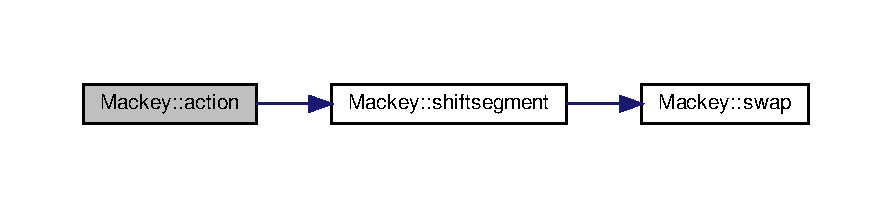
\includegraphics[width=350pt]{namespaceMackey_aa515b26c0fbc7f19b36cee7d826f07b9_cgraph}
\end{center}
\end{figure}
Here is the caller graph for this function\+:\nopagebreak
\begin{figure}[H]
\begin{center}
\leavevmode
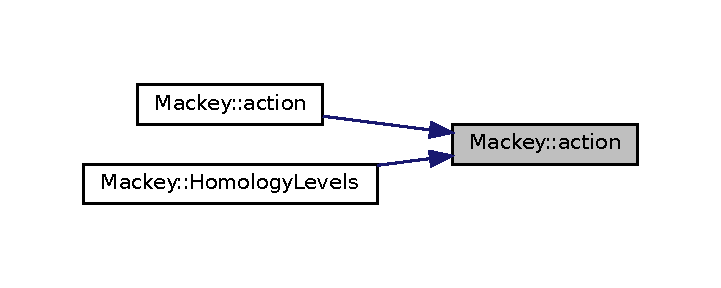
\includegraphics[width=346pt]{namespaceMackey_aa515b26c0fbc7f19b36cee7d826f07b9_icgraph}
\end{center}
\end{figure}
\mbox{\Hypertarget{namespaceMackey_aaa66c9857ba86a13949d1b1825ea20f7}\label{namespaceMackey_aaa66c9857ba86a13949d1b1825ea20f7}} 
\index{Mackey@{Mackey}!action@{action}}
\index{action@{action}!Mackey@{Mackey}}
\doxysubsubsection{\texorpdfstring{action()}{action()}\hspace{0.1cm}{\footnotesize\ttfamily [2/2]}}
{\footnotesize\ttfamily template$<$typename rank\+\_\+t , typename diff\+\_\+t $>$ \\
\mbox{\hyperlink{namespaceMackey_a035386035757dade630f685e508e5cf9}{mat\+\_\+t}}$<$rank\+\_\+t$>$ Mackey\+::action (\begin{DoxyParamCaption}\item[{const \mbox{\hyperlink{classMackey_1_1Homology}{Homology}}$<$ rank\+\_\+t, diff\+\_\+t $>$ \&}]{H,  }\item[{const rank\+\_\+t \&}]{rank }\end{DoxyParamCaption})}



Writing the Weyl group action on each generator in terms of the other generators. 

Here is the call graph for this function\+:\nopagebreak
\begin{figure}[H]
\begin{center}
\leavevmode
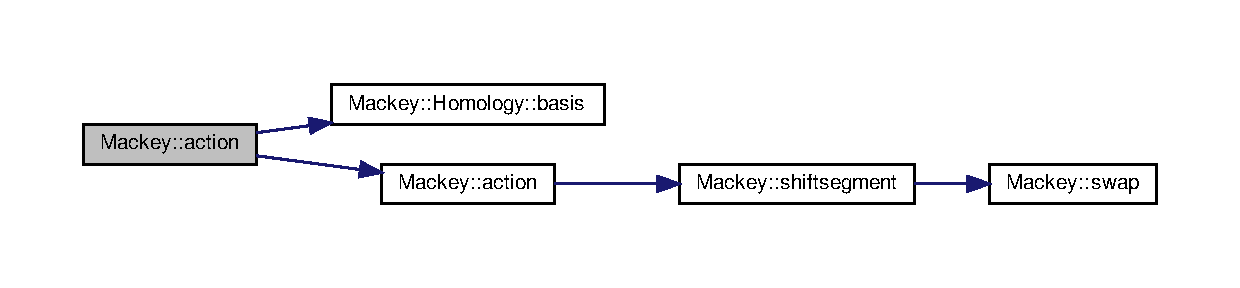
\includegraphics[width=350pt]{namespaceMackey_aaa66c9857ba86a13949d1b1825ea20f7_cgraph}
\end{center}
\end{figure}
\mbox{\Hypertarget{namespaceMackey_a2556e2a1f78783585df78de1c1b35eae}\label{namespaceMackey_a2556e2a1f78783585df78de1c1b35eae}} 
\index{Mackey@{Mackey}!all\_automorphisms@{all\_automorphisms}}
\index{all\_automorphisms@{all\_automorphisms}!Mackey@{Mackey}}
\doxysubsubsection{\texorpdfstring{all\_automorphisms()}{all\_automorphisms()}}
{\footnotesize\ttfamily template$<$typename T $>$ \\
std\+::pair$<$std\+::vector$<$\mbox{\hyperlink{namespaceMackey_a035386035757dade630f685e508e5cf9}{mat\+\_\+t}}$<$T$>$ $>$, std\+::vector$<$\mbox{\hyperlink{namespaceMackey_a035386035757dade630f685e508e5cf9}{mat\+\_\+t}}$<$T$>$ $>$ $>$ Mackey\+::all\+\_\+automorphisms (\begin{DoxyParamCaption}\item[{const T \&}]{Group }\end{DoxyParamCaption})}

Returns all automorphisms of a finitely generated abelian group together with their inverses. Currently only for p-\/groups and Z+p-\/groups (otherwise returns empty) Here is the call graph for this function\+:\nopagebreak
\begin{figure}[H]
\begin{center}
\leavevmode
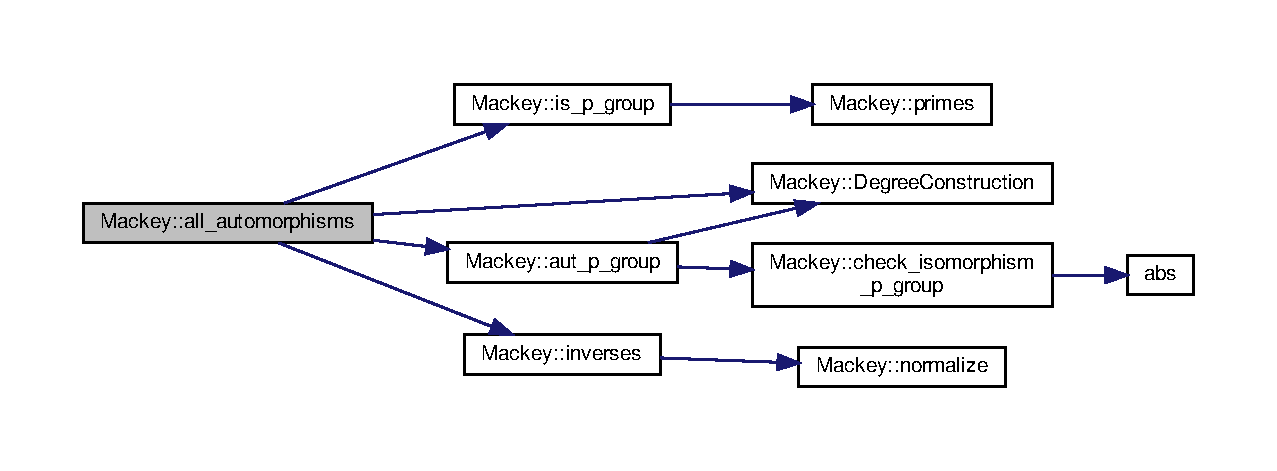
\includegraphics[width=350pt]{namespaceMackey_a2556e2a1f78783585df78de1c1b35eae_cgraph}
\end{center}
\end{figure}
Here is the caller graph for this function\+:\nopagebreak
\begin{figure}[H]
\begin{center}
\leavevmode
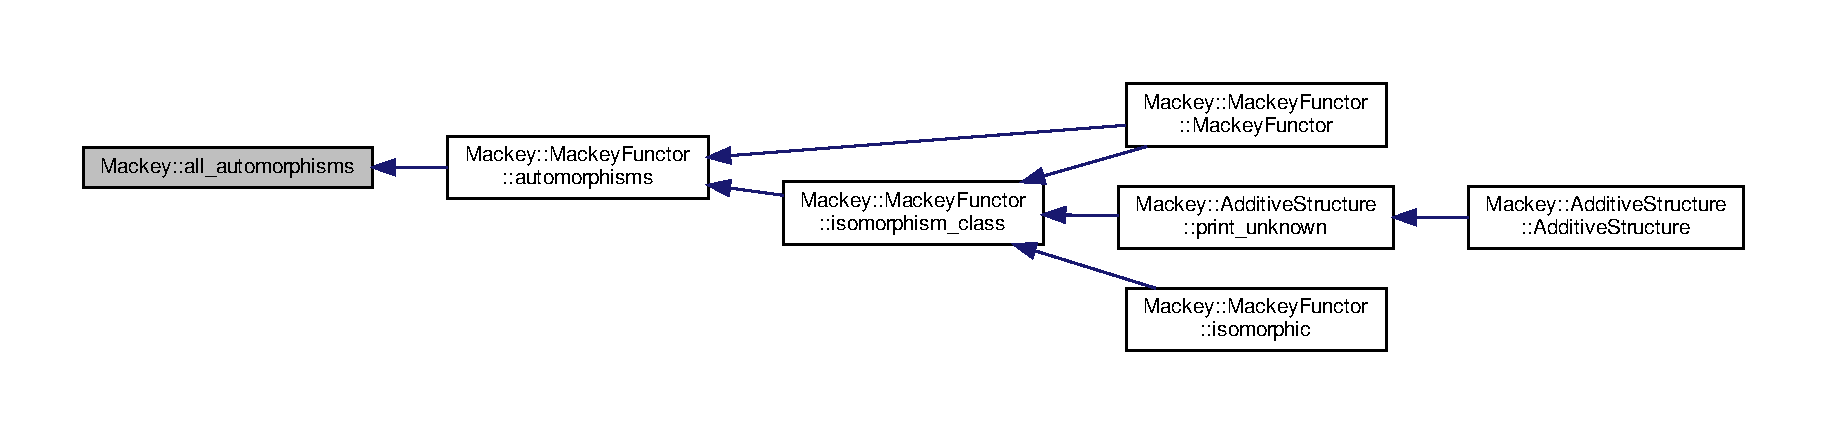
\includegraphics[width=350pt]{namespaceMackey_a2556e2a1f78783585df78de1c1b35eae_icgraph}
\end{center}
\end{figure}
\mbox{\Hypertarget{namespaceMackey_aa2f105c9bcbec7f5c7524027174340a0}\label{namespaceMackey_aa2f105c9bcbec7f5c7524027174340a0}} 
\index{Mackey@{Mackey}!altmatrix@{altmatrix}}
\index{altmatrix@{altmatrix}!Mackey@{Mackey}}
\doxysubsubsection{\texorpdfstring{altmatrix()}{altmatrix()}}
{\footnotesize\ttfamily template$<$typename Matrix\+\_\+t , std\+::enable\+\_\+if\+\_\+t$<$ S\+F\+I\+N\+A\+E\+::is\+\_\+\+Dense$<$ Matrix\+\_\+t $>$\+::value, int $>$  = 0$>$ \\
Matrix\+\_\+t Mackey\+::altmatrix (\begin{DoxyParamCaption}\item[{int}]{m,  }\item[{int}]{n,  }\item[{const std\+::vector$<$ \mbox{\hyperlink{namespaceMackey_a93ba297573961f91101fb84bc84bbe95}{Scalar\+\_\+t}}$<$ Matrix\+\_\+t $>$$>$ \&}]{v }\end{DoxyParamCaption})}



Creates a matrix of size m x n that alternates the given vector v. 

Sparse version of altmatrix.

Eg for m=2, n=2, v=\{a,b\} we get \{a,b // b,a\} Here is the call graph for this function\+:\nopagebreak
\begin{figure}[H]
\begin{center}
\leavevmode
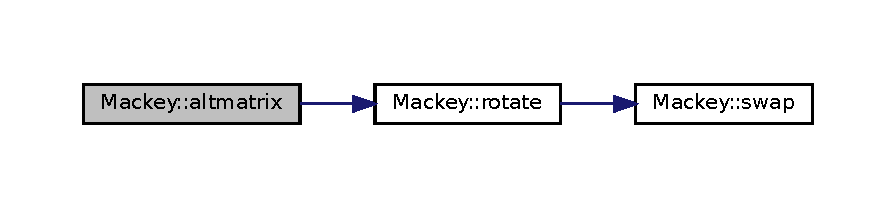
\includegraphics[width=350pt]{namespaceMackey_aa2f105c9bcbec7f5c7524027174340a0_cgraph}
\end{center}
\end{figure}
\mbox{\Hypertarget{namespaceMackey_a918f02198f6daadfd0c93109b63b2f1f}\label{namespaceMackey_a918f02198f6daadfd0c93109b63b2f1f}} 
\index{Mackey@{Mackey}!aut\_p\_group@{aut\_p\_group}}
\index{aut\_p\_group@{aut\_p\_group}!Mackey@{Mackey}}
\doxysubsubsection{\texorpdfstring{aut\_p\_group()}{aut\_p\_group()}}
{\footnotesize\ttfamily template$<$typename T $>$ \\
std\+::vector$<$\mbox{\hyperlink{namespaceMackey_a035386035757dade630f685e508e5cf9}{mat\+\_\+t}}$<$T$>$ $>$ Mackey\+::aut\+\_\+p\+\_\+group (\begin{DoxyParamCaption}\item[{int}]{p,  }\item[{const T \&}]{p\+Group }\end{DoxyParamCaption})}



Returns all automorphisms of finite abelian p-\/group. 

Here is the call graph for this function\+:\nopagebreak
\begin{figure}[H]
\begin{center}
\leavevmode
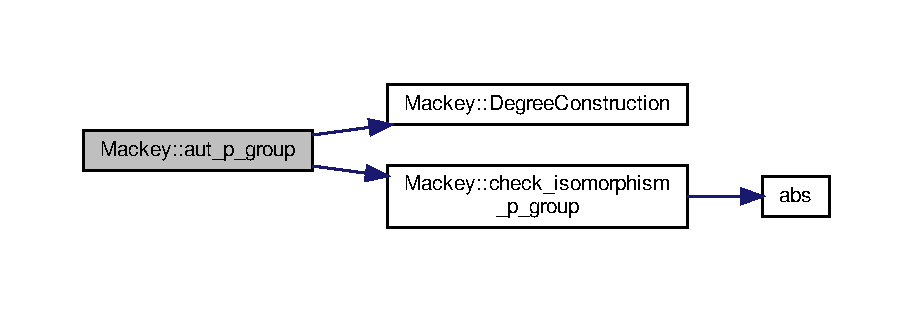
\includegraphics[width=350pt]{namespaceMackey_a918f02198f6daadfd0c93109b63b2f1f_cgraph}
\end{center}
\end{figure}
Here is the caller graph for this function\+:\nopagebreak
\begin{figure}[H]
\begin{center}
\leavevmode
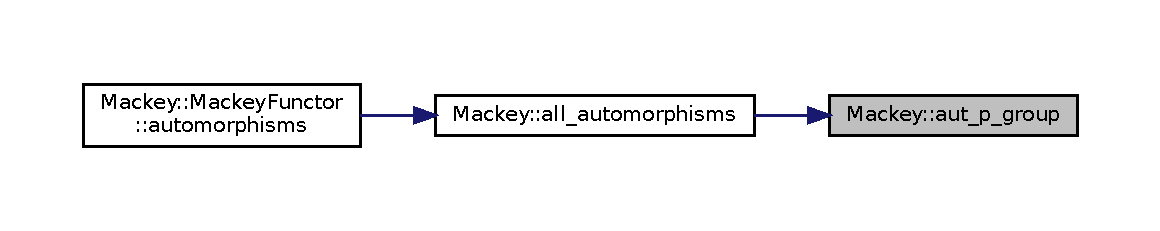
\includegraphics[width=350pt]{namespaceMackey_a918f02198f6daadfd0c93109b63b2f1f_icgraph}
\end{center}
\end{figure}
\mbox{\Hypertarget{namespaceMackey_aa10c6cbea565e024a38b446139800b69}\label{namespaceMackey_aa10c6cbea565e024a38b446139800b69}} 
\index{Mackey@{Mackey}!basisElement@{basisElement}}
\index{basisElement@{basisElement}!Mackey@{Mackey}}
\doxysubsubsection{\texorpdfstring{basisElement()}{basisElement()}\hspace{0.1cm}{\footnotesize\ttfamily [1/2]}}
{\footnotesize\ttfamily template$<$typename rank\+\_\+t $>$ \\
rank\+\_\+t Mackey\+::basis\+Element (\begin{DoxyParamCaption}\item[{int}]{length,  }\item[{int}]{position }\end{DoxyParamCaption})\hspace{0.3cm}{\ttfamily [inline]}}



Makes the the basis vector 0,...,1,...,0. 

\mbox{\Hypertarget{namespaceMackey_ac2e368bf7d802f2fc47e39a71a5a1630}\label{namespaceMackey_ac2e368bf7d802f2fc47e39a71a5a1630}} 
\index{Mackey@{Mackey}!basisElement@{basisElement}}
\index{basisElement@{basisElement}!Mackey@{Mackey}}
\doxysubsubsection{\texorpdfstring{basisElement()}{basisElement()}\hspace{0.1cm}{\footnotesize\ttfamily [2/2]}}
{\footnotesize\ttfamily template$<$typename rank\+\_\+t $>$ \\
rank\+\_\+t Mackey\+::basis\+Element (\begin{DoxyParamCaption}\item[{int}]{length,  }\item[{int}]{position,  }\item[{int}]{multiple }\end{DoxyParamCaption})\hspace{0.3cm}{\ttfamily [inline]}}



Makes the multiple of the basis vector 0,...,multiple,...,0. 

\mbox{\Hypertarget{namespaceMackey_a64d299f4b6f36e4b4e873b56a44b14b0}\label{namespaceMackey_a64d299f4b6f36e4b4e873b56a44b14b0}} 
\index{Mackey@{Mackey}!blockdiag@{blockdiag}}
\index{blockdiag@{blockdiag}!Mackey@{Mackey}}
\doxysubsubsection{\texorpdfstring{blockdiag()}{blockdiag()}\hspace{0.1cm}{\footnotesize\ttfamily [1/2]}}
{\footnotesize\ttfamily template$<$typename Matrix\+\_\+t $>$ \\
Matrix\+\_\+t Mackey\+::blockdiag (\begin{DoxyParamCaption}\item[{const Matrix\+\_\+t \&}]{A,  }\item[{const Matrix\+\_\+t \&}]{B }\end{DoxyParamCaption})}



The sum of two linear maps. 

Here is the call graph for this function\+:\nopagebreak
\begin{figure}[H]
\begin{center}
\leavevmode
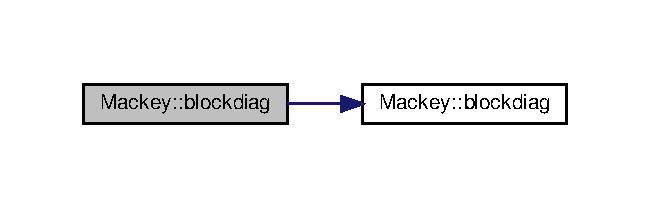
\includegraphics[width=330pt]{namespaceMackey_a64d299f4b6f36e4b4e873b56a44b14b0_cgraph}
\end{center}
\end{figure}
\mbox{\Hypertarget{namespaceMackey_a6d2d912037da84c6884ac62db997cc0f}\label{namespaceMackey_a6d2d912037da84c6884ac62db997cc0f}} 
\index{Mackey@{Mackey}!blockdiag@{blockdiag}}
\index{blockdiag@{blockdiag}!Mackey@{Mackey}}
\doxysubsubsection{\texorpdfstring{blockdiag()}{blockdiag()}\hspace{0.1cm}{\footnotesize\ttfamily [2/2]}}
{\footnotesize\ttfamily template$<$typename Matrix\+\_\+t $>$ \\
Matrix\+\_\+t Mackey\+::blockdiag (\begin{DoxyParamCaption}\item[{const Matrix\+\_\+t \&}]{A,  }\item[{const Matrix\+\_\+t \&}]{B,  }\item[{int}]{domA,  }\item[{int}]{ranA,  }\item[{int}]{domB,  }\item[{int}]{ranB }\end{DoxyParamCaption})}



The sum of two linear maps. We account for a map being empty if domain/range is 0 hence why the dimensions of domains and ranges are given. 

Here is the caller graph for this function\+:\nopagebreak
\begin{figure}[H]
\begin{center}
\leavevmode
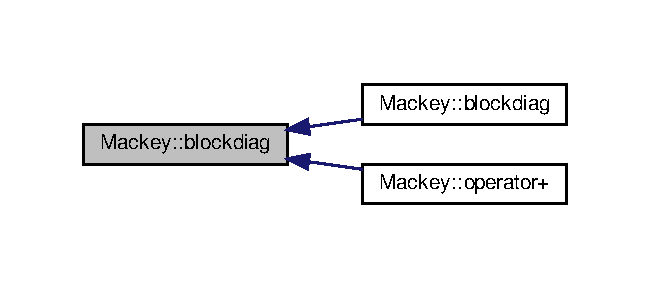
\includegraphics[width=332pt]{namespaceMackey_a6d2d912037da84c6884ac62db997cc0f_icgraph}
\end{center}
\end{figure}
\mbox{\Hypertarget{namespaceMackey_a72abbe3708c4e77936c8cc42fbc6753a}\label{namespaceMackey_a72abbe3708c4e77936c8cc42fbc6753a}} 
\index{Mackey@{Mackey}!Box@{Box}}
\index{Box@{Box}!Mackey@{Mackey}}
\doxysubsubsection{\texorpdfstring{Box()}{Box()}\hspace{0.1cm}{\footnotesize\ttfamily [1/2]}}
{\footnotesize\ttfamily template$<$typename rank\+\_\+t , typename diff\+\_\+t $>$ \\
\mbox{\hyperlink{classMackey_1_1Chains}{Chains}}$<$rank\+\_\+t, diff\+\_\+t$>$ Mackey\+::\+Box (\begin{DoxyParamCaption}\item[{const \mbox{\hyperlink{classMackey_1_1Chains}{Chains}}$<$ rank\+\_\+t, diff\+\_\+t $>$ \&}]{C,  }\item[{const \mbox{\hyperlink{classMackey_1_1Chains}{Chains}}$<$ rank\+\_\+t, diff\+\_\+t $>$ \&}]{D }\end{DoxyParamCaption})\hspace{0.3cm}{\ttfamily [inline]}}



Get the entire box product of C,D. 

\mbox{\Hypertarget{namespaceMackey_add5b60c8e734df2be261106e0c719f82}\label{namespaceMackey_add5b60c8e734df2be261106e0c719f82}} 
\index{Mackey@{Mackey}!Box@{Box}}
\index{Box@{Box}!Mackey@{Mackey}}
\doxysubsubsection{\texorpdfstring{Box()}{Box()}\hspace{0.1cm}{\footnotesize\ttfamily [2/2]}}
{\footnotesize\ttfamily template$<$typename rank\+\_\+t , typename diff\+\_\+t $>$ \\
\mbox{\hyperlink{classMackey_1_1Chains}{Chains}}$<$rank\+\_\+t, diff\+\_\+t$>$ Mackey\+::\+Box (\begin{DoxyParamCaption}\item[{const \mbox{\hyperlink{classMackey_1_1Chains}{Chains}}$<$ rank\+\_\+t, diff\+\_\+t $>$ \&}]{C,  }\item[{const \mbox{\hyperlink{classMackey_1_1Chains}{Chains}}$<$ rank\+\_\+t, diff\+\_\+t $>$ \&}]{D,  }\item[{int}]{i }\end{DoxyParamCaption})\hspace{0.3cm}{\ttfamily [inline]}}



Get the box product of C,D up to index i. 

Here is the caller graph for this function\+:\nopagebreak
\begin{figure}[H]
\begin{center}
\leavevmode
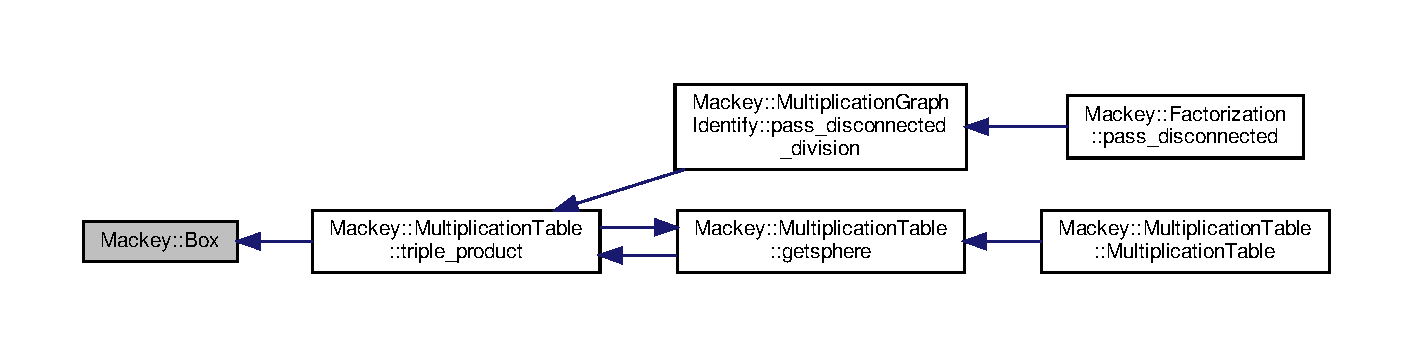
\includegraphics[width=350pt]{namespaceMackey_add5b60c8e734df2be261106e0c719f82_icgraph}
\end{center}
\end{figure}
\mbox{\Hypertarget{namespaceMackey_a94aab405619cb172fe79ab5fc68a4fac}\label{namespaceMackey_a94aab405619cb172fe79ab5fc68a4fac}} 
\index{Mackey@{Mackey}!box\_sparse@{box\_sparse}}
\index{box\_sparse@{box\_sparse}!Mackey@{Mackey}}
\doxysubsubsection{\texorpdfstring{box\_sparse()}{box\_sparse()}}
{\footnotesize\ttfamily template$<$typename T , typename S , typename storage , typename U , typename V $>$ \\
void Mackey\+::box\+\_\+sparse (\begin{DoxyParamCaption}\item[{\mbox{\hyperlink{namespaceMackey_a0b8cd52f81199d53fa1e93946d8115ef}{triplets}}$<$ T, storage $>$ \&}]{trip,  }\item[{const S \&}]{left,  }\item[{const S \&}]{right,  }\item[{const \mbox{\hyperlink{namespaceMackey_a0b8cd52f81199d53fa1e93946d8115ef}{triplets}}$<$ T, storage $>$ \&}]{a,  }\item[{U}]{rows,  }\item[{U}]{cols,  }\item[{V}]{copies,  }\item[{storage}]{h\+\_\+offset,  }\item[{storage}]{v\+\_\+offset }\end{DoxyParamCaption})}



Does permutation\+\_\+block and matrix mixing in one step for sparse matrices, using the triplets format. 

\mbox{\Hypertarget{namespaceMackey_a232e85ca1fb9017788b33b7f6f2c269b}\label{namespaceMackey_a232e85ca1fb9017788b33b7f6f2c269b}} 
\index{Mackey@{Mackey}!boxchangebasis@{boxchangebasis}}
\index{boxchangebasis@{boxchangebasis}!Mackey@{Mackey}}
\doxysubsubsection{\texorpdfstring{boxchangebasis()}{boxchangebasis()}}
{\footnotesize\ttfamily template$<$typename p\+Scalar , typename rank\+\_\+t $>$ \\
std\+::pair$<$std\+::vector$<$p\+Scalar$>$, std\+::vector$<$p\+Scalar$>$ $>$ Mackey\+::boxchangebasis (\begin{DoxyParamCaption}\item[{const rank\+\_\+t \&}]{rankC,  }\item[{const rank\+\_\+t \&}]{rankD,  }\item[{bool}]{convtocanon }\end{DoxyParamCaption})}



Constructs the 3 bases (left+right convenient and canonical) and returns the two change of basis matrices (as permutations). 

Here is the call graph for this function\+:\nopagebreak
\begin{figure}[H]
\begin{center}
\leavevmode
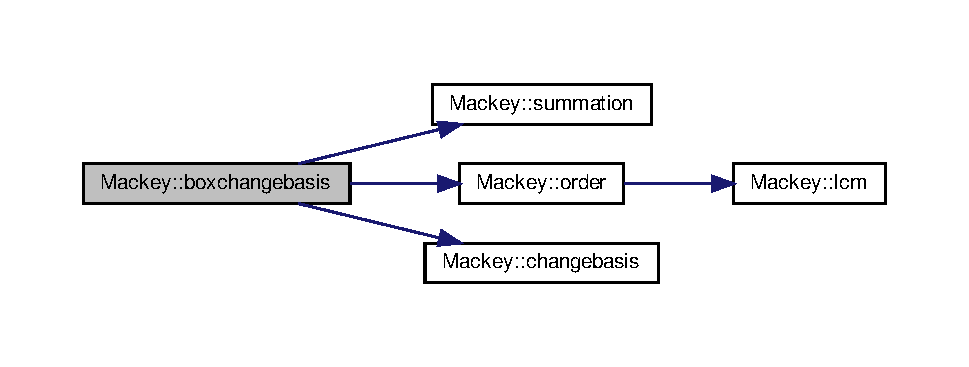
\includegraphics[width=350pt]{namespaceMackey_a232e85ca1fb9017788b33b7f6f2c269b_cgraph}
\end{center}
\end{figure}
\mbox{\Hypertarget{namespaceMackey_a65dac6a38a02a4efc56d52292ea8cbd8}\label{namespaceMackey_a65dac6a38a02a4efc56d52292ea8cbd8}} 
\index{Mackey@{Mackey}!change\_base\_matrix\_normalize@{change\_base\_matrix\_normalize}}
\index{change\_base\_matrix\_normalize@{change\_base\_matrix\_normalize}!Mackey@{Mackey}}
\doxysubsubsection{\texorpdfstring{change\_base\_matrix\_normalize()}{change\_base\_matrix\_normalize()}}
{\footnotesize\ttfamily template$<$typename T , typename S $>$ \\
T Mackey\+::change\+\_\+base\+\_\+matrix\+\_\+normalize (\begin{DoxyParamCaption}\item[{const T \&}]{mat,  }\item[{const T \&}]{P,  }\item[{const T \&}]{Q,  }\item[{const S \&}]{Group\+\_\+image }\end{DoxyParamCaption})}



Given matrix and change of basis matrices, produces the matrix w.\+r.\+t. the new basis and normalizes it for the given group in the image. 

Here is the call graph for this function\+:\nopagebreak
\begin{figure}[H]
\begin{center}
\leavevmode
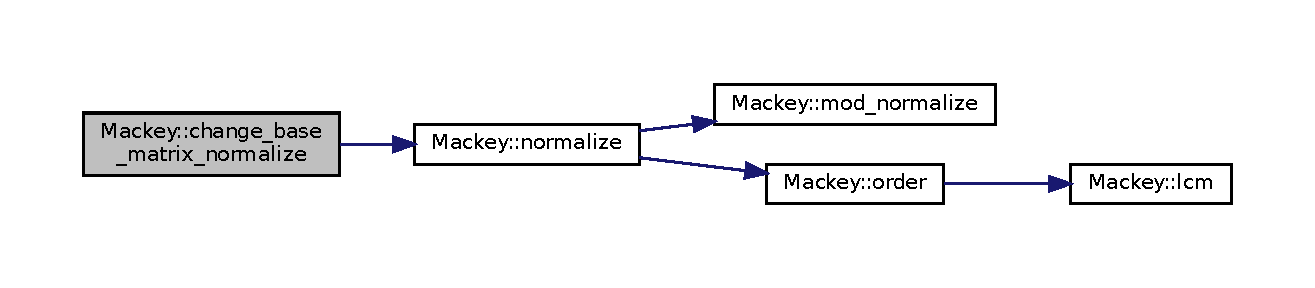
\includegraphics[width=350pt]{namespaceMackey_a65dac6a38a02a4efc56d52292ea8cbd8_cgraph}
\end{center}
\end{figure}
Here is the caller graph for this function\+:\nopagebreak
\begin{figure}[H]
\begin{center}
\leavevmode
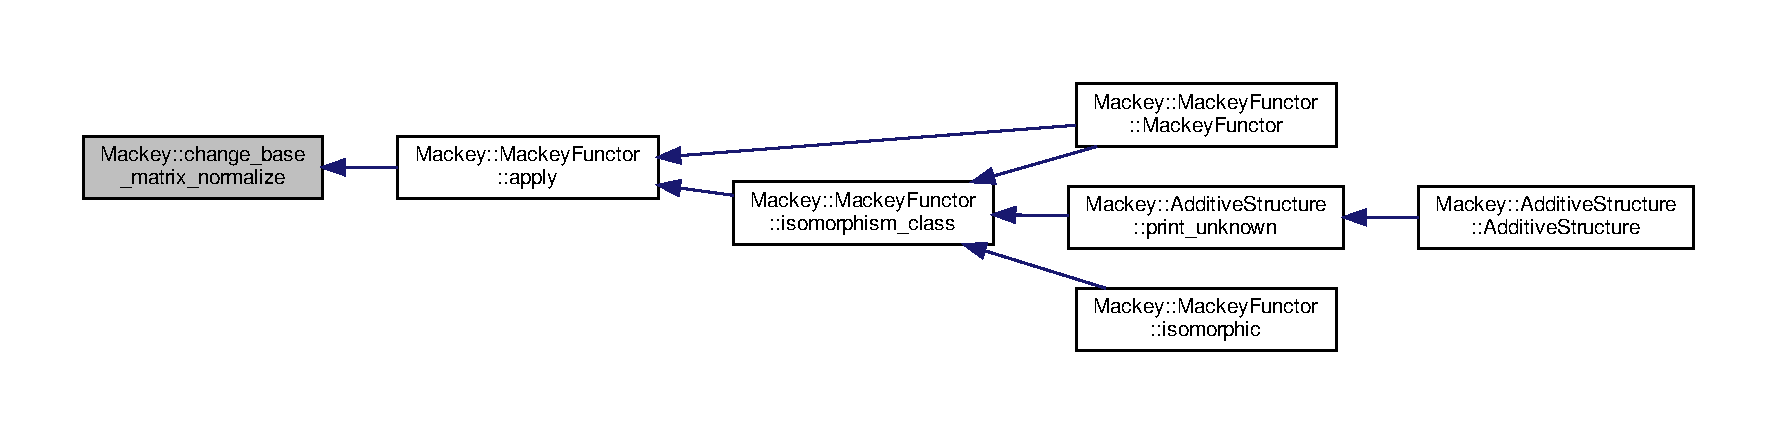
\includegraphics[width=350pt]{namespaceMackey_a65dac6a38a02a4efc56d52292ea8cbd8_icgraph}
\end{center}
\end{figure}
\mbox{\Hypertarget{namespaceMackey_a15de590d1a5126349995e6649be29ff2}\label{namespaceMackey_a15de590d1a5126349995e6649be29ff2}} 
\index{Mackey@{Mackey}!changebasis@{changebasis}}
\index{changebasis@{changebasis}!Mackey@{Mackey}}
\doxysubsubsection{\texorpdfstring{changebasis()}{changebasis()}}
{\footnotesize\ttfamily template$<$typename p\+Scalar , typename T $>$ \\
std\+::vector$<$p\+Scalar$>$ Mackey\+::changebasis (\begin{DoxyParamCaption}\item[{const std\+::vector$<$ T $>$ \&}]{A,  }\item[{const std\+::vector$<$ T $>$ \&}]{B }\end{DoxyParamCaption})}



Returns the change of basis matrix (as a permutation) from basis A to basis B. 

\mbox{\Hypertarget{namespaceMackey_aa96cf972d89b207ce6709e867f760f37}\label{namespaceMackey_aa96cf972d89b207ce6709e867f760f37}} 
\index{Mackey@{Mackey}!check\_isomorphism\_p\_group@{check\_isomorphism\_p\_group}}
\index{check\_isomorphism\_p\_group@{check\_isomorphism\_p\_group}!Mackey@{Mackey}}
\doxysubsubsection{\texorpdfstring{check\_isomorphism\_p\_group()}{check\_isomorphism\_p\_group()}}
{\footnotesize\ttfamily template$<$typename T , typename S $>$ \\
bool Mackey\+::check\+\_\+isomorphism\+\_\+p\+\_\+group (\begin{DoxyParamCaption}\item[{int}]{p,  }\item[{const T \&}]{a,  }\item[{const S \&}]{p\+Group }\end{DoxyParamCaption})}



Checks if integer matrix induces an isomorphism p\+Group-\/$>$p\+Group for finite abelian p-\/group. 

Here is the call graph for this function\+:\nopagebreak
\begin{figure}[H]
\begin{center}
\leavevmode
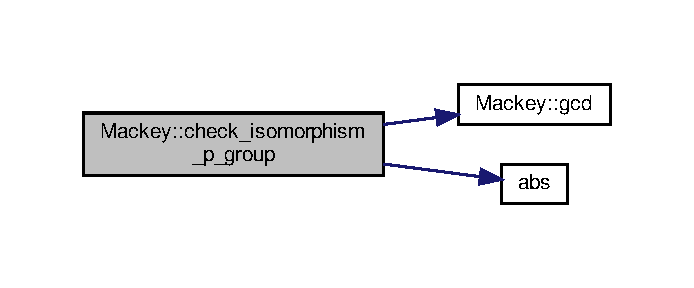
\includegraphics[width=307pt]{namespaceMackey_aa96cf972d89b207ce6709e867f760f37_cgraph}
\end{center}
\end{figure}
Here is the caller graph for this function\+:\nopagebreak
\begin{figure}[H]
\begin{center}
\leavevmode
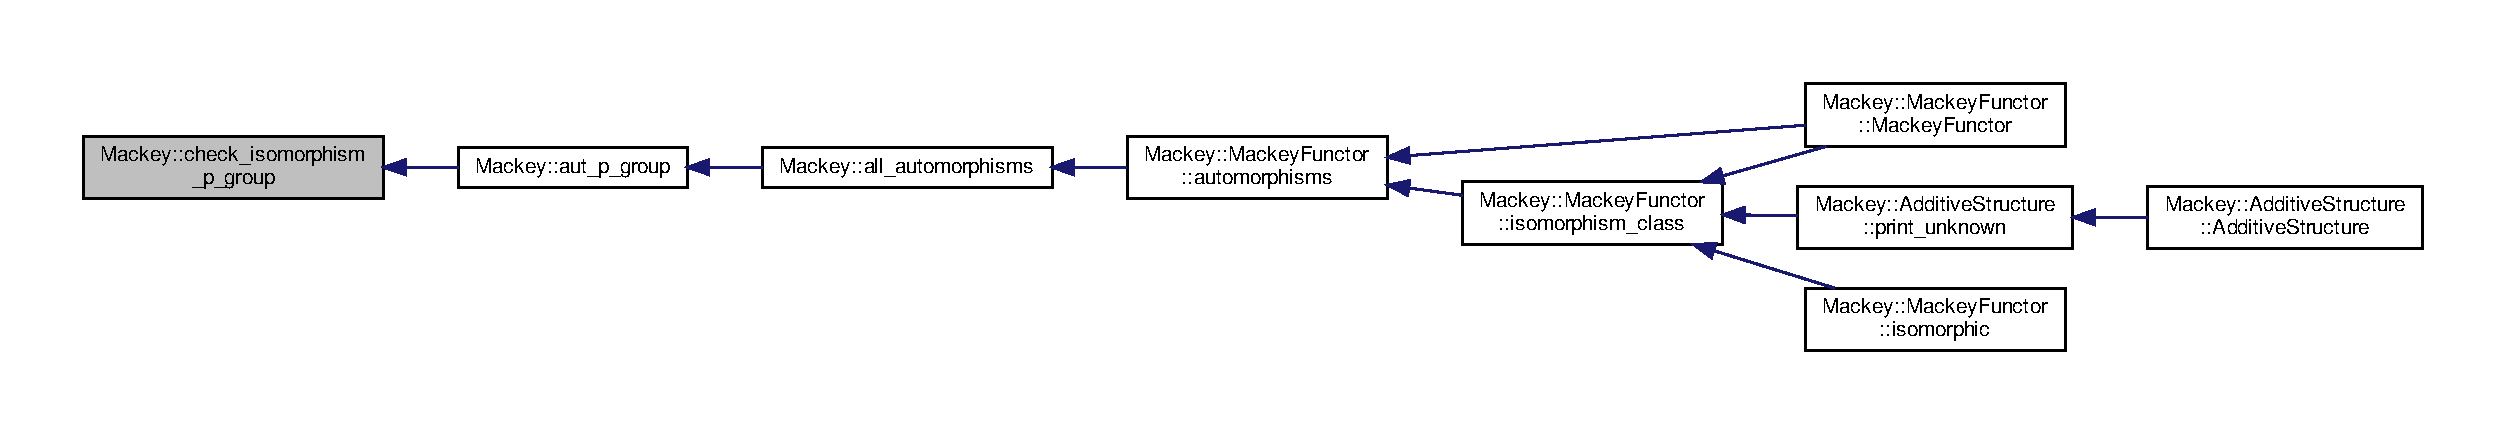
\includegraphics[width=350pt]{namespaceMackey_aa96cf972d89b207ce6709e867f760f37_icgraph}
\end{center}
\end{figure}
\mbox{\Hypertarget{namespaceMackey_a3a4b7761ed7274b145eed9a451b53e61}\label{namespaceMackey_a3a4b7761ed7274b145eed9a451b53e61}} 
\index{Mackey@{Mackey}!combinations@{combinations}}
\index{combinations@{combinations}!Mackey@{Mackey}}
\doxysubsubsection{\texorpdfstring{combinations()}{combinations()}}
{\footnotesize\ttfamily template$<$typename T $>$ \\
std\+::vector$<$std\+::vector$<$T$>$ $>$ Mackey\+::combinations (\begin{DoxyParamCaption}\item[{const std\+::vector$<$ std\+::vector$<$ T $>$$>$ \&}]{v }\end{DoxyParamCaption})}



Given a vector of vectors v form all combinations of the form \{v\mbox{[}0\mbox{]}\mbox{[}?\mbox{]},v\mbox{[}1\mbox{]}\mbox{[}?\mbox{]},...\} for varying ? 

Here is the caller graph for this function\+:\nopagebreak
\begin{figure}[H]
\begin{center}
\leavevmode
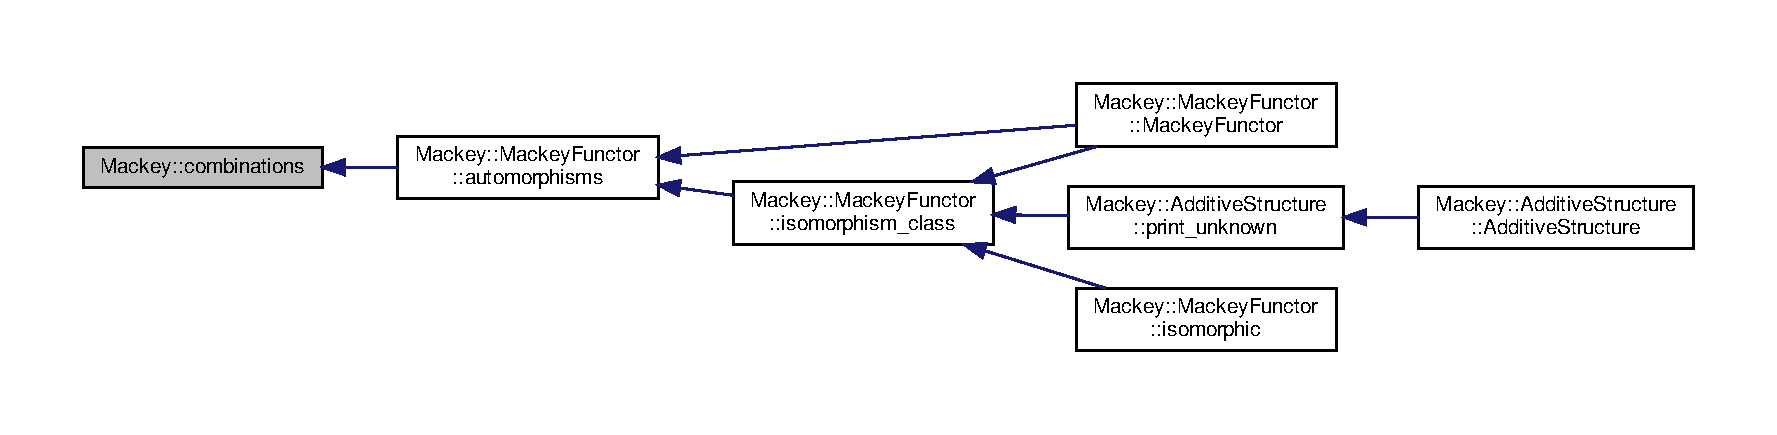
\includegraphics[width=350pt]{namespaceMackey_a3a4b7761ed7274b145eed9a451b53e61_icgraph}
\end{center}
\end{figure}
\mbox{\Hypertarget{namespaceMackey_a49fef6f64b67ff118d35ac45b9c92972}\label{namespaceMackey_a49fef6f64b67ff118d35ac45b9c92972}} 
\index{Mackey@{Mackey}!DegreeConstruction@{DegreeConstruction}}
\index{DegreeConstruction@{DegreeConstruction}!Mackey@{Mackey}}
\doxysubsubsection{\texorpdfstring{DegreeConstruction()}{DegreeConstruction()}}
{\footnotesize\ttfamily template$<$typename deg\+\_\+t  = std\+::vector$<$int$>$$>$ \\
std\+::vector$<$deg\+\_\+t$>$ Mackey\+::\+Degree\+Construction (\begin{DoxyParamCaption}\item[{const deg\+\_\+t \&}]{minimum,  }\item[{const deg\+\_\+t \&}]{maximum }\end{DoxyParamCaption})}



Given minimum and maximum degrees, constructs everything in between. 

For example if minimum=\{-\/1,-\/1\} and maximum=\{2,3\} then the result is \{\{-\/1,-\/1\},\{0,-\/1\},\{1,-\/1\},\{2,-\/1\},\{-\/1,0\},...,\{2,3\}\} Here is the caller graph for this function\+:\nopagebreak
\begin{figure}[H]
\begin{center}
\leavevmode
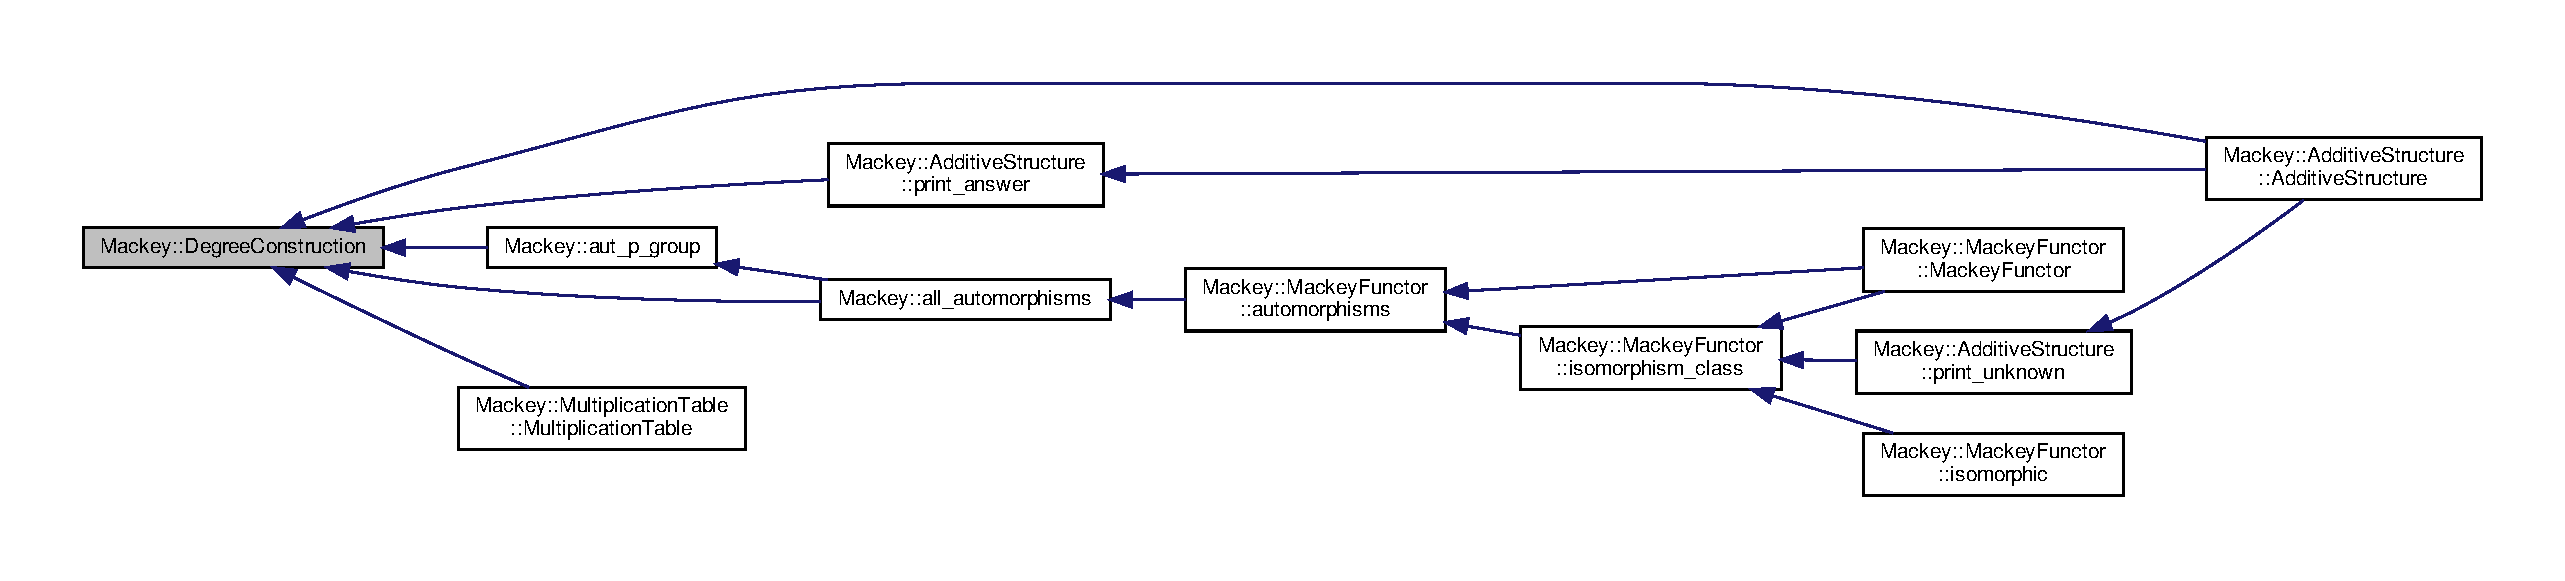
\includegraphics[width=350pt]{namespaceMackey_a49fef6f64b67ff118d35ac45b9c92972_icgraph}
\end{center}
\end{figure}
\mbox{\Hypertarget{namespaceMackey_a2f26791310db25c7e42bf5341fdfd48d}\label{namespaceMackey_a2f26791310db25c7e42bf5341fdfd48d}} 
\index{Mackey@{Mackey}!diagonalize@{diagonalize}}
\index{diagonalize@{diagonalize}!Mackey@{Mackey}}
\doxysubsubsection{\texorpdfstring{diagonalize()}{diagonalize()}\hspace{0.1cm}{\footnotesize\ttfamily [1/2]}}
{\footnotesize\ttfamily template$<$typename S\+\_\+t , typename R\+\_\+t , typename C\+\_\+t $>$ \\
\mbox{\hyperlink{classMackey_1_1Smith}{Smith}}$<$S\+\_\+t, R\+\_\+t, C\+\_\+t$>$ Mackey\+::diagonalize (\begin{DoxyParamCaption}\item[{const S\+\_\+t \&}]{A,  }\item[{bool}]{wantP,  }\item[{bool}]{wantQ }\end{DoxyParamCaption})}



Returns the unsorted \mbox{\hyperlink{classMackey_1_1Smith}{Smith}} Normal Form of a matrix, with the coefficient matrices if desired. 

\mbox{\Hypertarget{namespaceMackey_a276ffc8b4c9c52cfde39cd3da3c88cc9}\label{namespaceMackey_a276ffc8b4c9c52cfde39cd3da3c88cc9}} 
\index{Mackey@{Mackey}!diagonalize@{diagonalize}}
\index{diagonalize@{diagonalize}!Mackey@{Mackey}}
\doxysubsubsection{\texorpdfstring{diagonalize()}{diagonalize()}\hspace{0.1cm}{\footnotesize\ttfamily [2/2]}}
{\footnotesize\ttfamily template$<$typename S\+\_\+t , typename R\+\_\+t , typename C\+\_\+t $>$ \\
\mbox{\hyperlink{classMackey_1_1Smith}{Smith}}$<$S\+\_\+t, R\+\_\+t, C\+\_\+t$>$ Mackey\+::diagonalize (\begin{DoxyParamCaption}\item[{const S\+\_\+t \&}]{A,  }\item[{bool}]{wantP,  }\item[{bool}]{wantQ,  }\item[{bool}]{sort }\end{DoxyParamCaption})}



Returns the \mbox{\hyperlink{classMackey_1_1Smith}{Smith}} Normal Form of a matrix, with the coefficient matrices and sorted if desired. 

\mbox{\Hypertarget{namespaceMackey_a6a5d40e69e5628ea84896ee43f4a91fa}\label{namespaceMackey_a6a5d40e69e5628ea84896ee43f4a91fa}} 
\index{Mackey@{Mackey}!dimension@{dimension}}
\index{dimension@{dimension}!Mackey@{Mackey}}
\doxysubsubsection{\texorpdfstring{dimension()}{dimension()}}
{\footnotesize\ttfamily template$<$typename deg\+\_\+t $>$ \\
int Mackey\+::dimension (\begin{DoxyParamCaption}\item[{const deg\+\_\+t \&}]{sphere }\end{DoxyParamCaption})\hspace{0.3cm}{\ttfamily [inline]}}



Compute the dimension of a representation sphere. 

Here is the call graph for this function\+:\nopagebreak
\begin{figure}[H]
\begin{center}
\leavevmode
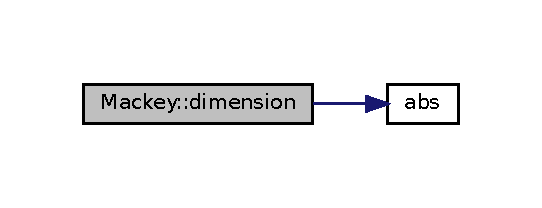
\includegraphics[width=260pt]{namespaceMackey_a6a5d40e69e5628ea84896ee43f4a91fa_cgraph}
\end{center}
\end{figure}
Here is the caller graph for this function\+:\nopagebreak
\begin{figure}[H]
\begin{center}
\leavevmode
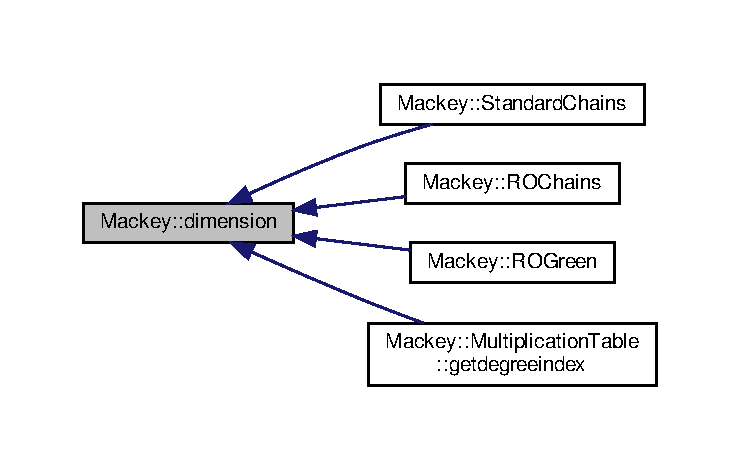
\includegraphics[width=350pt]{namespaceMackey_a6a5d40e69e5628ea84896ee43f4a91fa_icgraph}
\end{center}
\end{figure}
\mbox{\Hypertarget{namespaceMackey_a281b9be315d7d51c7e691d4c733ac0c9}\label{namespaceMackey_a281b9be315d7d51c7e691d4c733ac0c9}} 
\index{Mackey@{Mackey}!distinguish@{distinguish}}
\index{distinguish@{distinguish}!Mackey@{Mackey}}
\doxysubsubsection{\texorpdfstring{distinguish()}{distinguish()}}
{\footnotesize\ttfamily template$<$typename rank\+\_\+t $>$ \\
bool Mackey\+::distinguish (\begin{DoxyParamCaption}\item[{const std\+::vector$<$ rank\+\_\+t $>$ \&}]{elements,  }\item[{const \mbox{\hyperlink{classMackey_1_1IDGenerators}{I\+D\+Generators}}$<$ rank\+\_\+t $>$ \&}]{Id }\end{DoxyParamCaption})}



Find if given elements can all be distinguished i.\+e. they have pairwise disjoint candidate sets. 

Here is the call graph for this function\+:\nopagebreak
\begin{figure}[H]
\begin{center}
\leavevmode
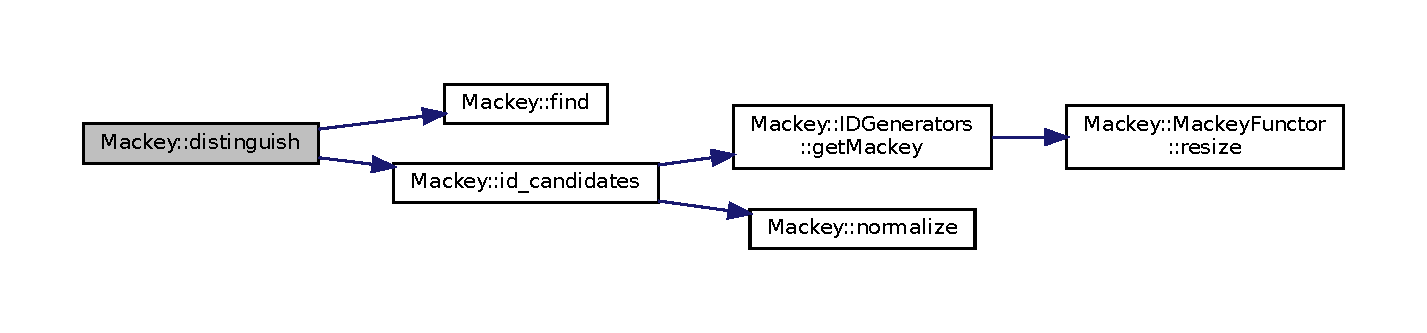
\includegraphics[width=350pt]{namespaceMackey_a281b9be315d7d51c7e691d4c733ac0c9_cgraph}
\end{center}
\end{figure}
\mbox{\Hypertarget{namespaceMackey_a55e12d500b5495a1949b212533c622be}\label{namespaceMackey_a55e12d500b5495a1949b212533c622be}} 
\index{Mackey@{Mackey}!equidistribute@{equidistribute}}
\index{equidistribute@{equidistribute}!Mackey@{Mackey}}
\doxysubsubsection{\texorpdfstring{equidistribute()}{equidistribute()}}
{\footnotesize\ttfamily template$<$typename T $>$ \\
std\+::vector$<$std\+::vector$<$int$>$ $>$ Mackey\+::equidistribute (\begin{DoxyParamCaption}\item[{const std\+::vector$<$ int $>$ \&}]{weights,  }\item[{const std\+::vector$<$ T $>$ \&}]{items,  }\item[{int}]{no\+\_\+teams }\end{DoxyParamCaption})}



Distribute evenly among teams as much as possible (greedy solution to partition problem) 

\mbox{\Hypertarget{namespaceMackey_a91104eaef1ab349e68f0623cfaaf45c0}\label{namespaceMackey_a91104eaef1ab349e68f0623cfaaf45c0}} 
\index{Mackey@{Mackey}!find@{find}}
\index{find@{find}!Mackey@{Mackey}}
\doxysubsubsection{\texorpdfstring{find()}{find()}}
{\footnotesize\ttfamily template$<$typename T , typename S , std\+::enable\+\_\+if\+\_\+t$<$!\+S\+F\+I\+N\+A\+E\+::is\+\_\+\+Dense$<$ S $>$\+::value, int $>$  = 0$>$ \\
int Mackey\+::find (\begin{DoxyParamCaption}\item[{const T \&}]{v,  }\item[{const S \&}]{a }\end{DoxyParamCaption})}



Find first instance of a in v for non \mbox{\hyperlink{namespaceEigen}{Eigen}} matrices. 

Find first instance of a in v for dense \mbox{\hyperlink{namespaceEigen}{Eigen}} matrices. Here is the caller graph for this function\+:\nopagebreak
\begin{figure}[H]
\begin{center}
\leavevmode
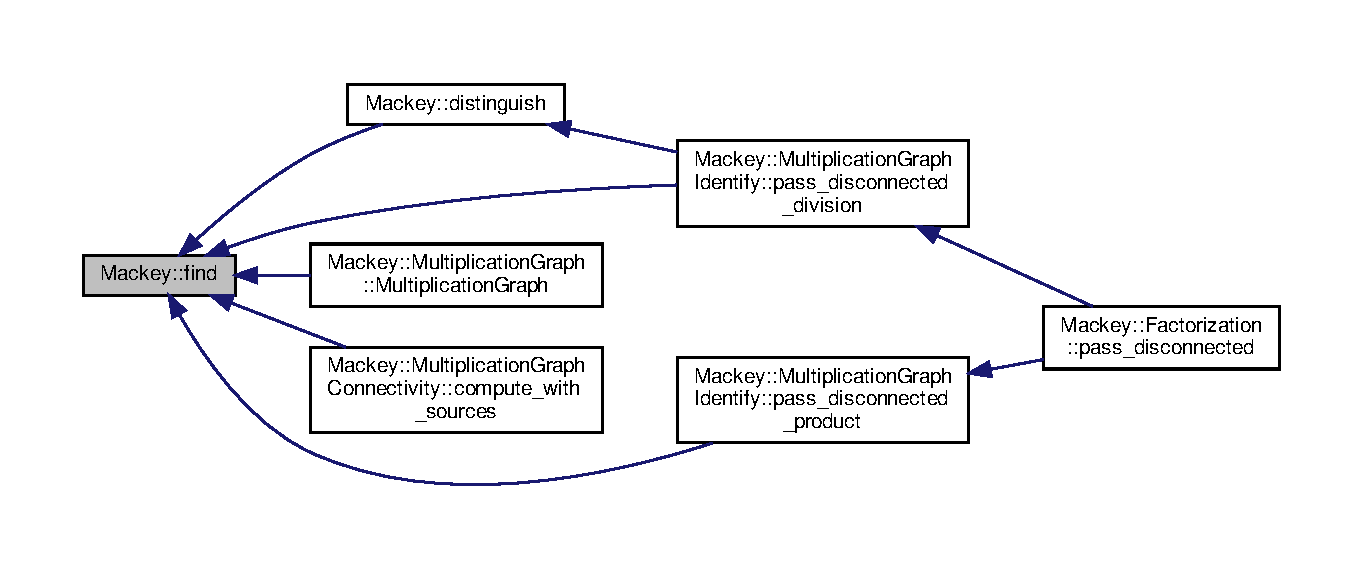
\includegraphics[width=348pt]{namespaceMackey_a91104eaef1ab349e68f0623cfaaf45c0_icgraph}
\end{center}
\end{figure}
\mbox{\Hypertarget{namespaceMackey_a3d23281b881eb1f166107b333fa98612}\label{namespaceMackey_a3d23281b881eb1f166107b333fa98612}} 
\index{Mackey@{Mackey}!hashvector@{hashvector}}
\index{hashvector@{hashvector}!Mackey@{Mackey}}
\doxysubsubsection{\texorpdfstring{hashvector()}{hashvector()}}
{\footnotesize\ttfamily template$<$typename T $>$ \\
long Mackey\+::hashvector (\begin{DoxyParamCaption}\item[{const T \&}]{deg,  }\item[{const T \&}]{min,  }\item[{const T \&}]{max }\end{DoxyParamCaption})}



Hash vector given minimum and maximum values of its entries. 

\mbox{\Hypertarget{namespaceMackey_a1c195484cc947abef84c726b534af5a5}\label{namespaceMackey_a1c195484cc947abef84c726b534af5a5}} 
\index{Mackey@{Mackey}!HomologyLevels@{HomologyLevels}}
\index{HomologyLevels@{HomologyLevels}!Mackey@{Mackey}}
\doxysubsubsection{\texorpdfstring{HomologyLevels()}{HomologyLevels()}}
{\footnotesize\ttfamily template$<$typename rank\+\_\+t , typename diff\+\_\+t $>$ \\
\mbox{\hyperlink{classMackey_1_1MackeyFunctor}{Mackey\+Functor}}$<$rank\+\_\+t$>$ Mackey\+::\+Homology\+Levels (\begin{DoxyParamCaption}\item[{const \mbox{\hyperlink{classMackey_1_1Levels}{Levels}}$<$ \mbox{\hyperlink{classMackey_1_1Junction}{Junction}}$<$ rank\+\_\+t, diff\+\_\+t $>$ $>$ \&}]{J }\end{DoxyParamCaption})}



The \mbox{\hyperlink{namespaceMackey}{Mackey}} functor \mbox{\hyperlink{classMackey_1_1Homology}{Homology}} of a \mbox{\hyperlink{classMackey_1_1Junction}{Junction}} of \mbox{\hyperlink{namespaceMackey}{Mackey}} functors. 

Here is the call graph for this function\+:\nopagebreak
\begin{figure}[H]
\begin{center}
\leavevmode
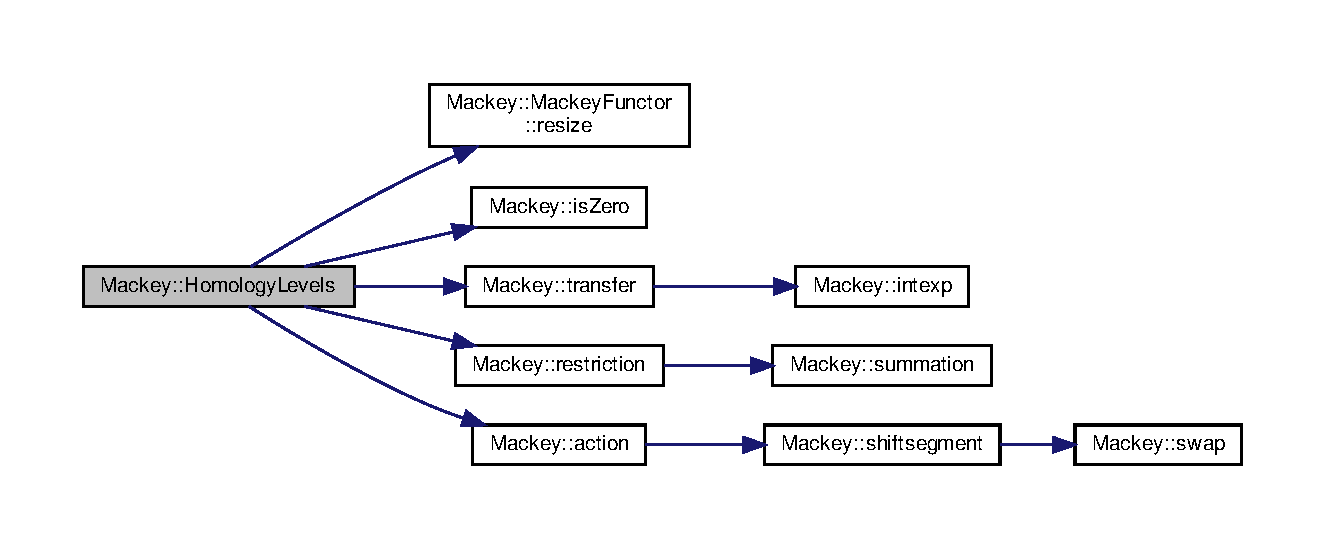
\includegraphics[width=350pt]{namespaceMackey_a1c195484cc947abef84c726b534af5a5_cgraph}
\end{center}
\end{figure}
\mbox{\Hypertarget{namespaceMackey_a83ac78e6d1695af40d0fa58af5255e84}\label{namespaceMackey_a83ac78e6d1695af40d0fa58af5255e84}} 
\index{Mackey@{Mackey}!id\_candidates@{id\_candidates}}
\index{id\_candidates@{id\_candidates}!Mackey@{Mackey}}
\doxysubsubsection{\texorpdfstring{id\_candidates()}{id\_candidates()}}
{\footnotesize\ttfamily template$<$typename rank\+\_\+t $>$ \\
std\+::vector$<$rank\+\_\+t$>$ Mackey\+::id\+\_\+candidates (\begin{DoxyParamCaption}\item[{const rank\+\_\+t \&}]{basis,  }\item[{const \mbox{\hyperlink{classMackey_1_1IDGenerators}{I\+D\+Generators}}$<$ rank\+\_\+t $>$ \&}]{Id\+\_\+first,  }\item[{const \mbox{\hyperlink{classMackey_1_1IDGenerators}{I\+D\+Generators}}$<$ rank\+\_\+t $>$ \&}]{Id\+\_\+second }\end{DoxyParamCaption})}



Use the ID data to identify all possible candidates for an element. 

Here is the call graph for this function\+:\nopagebreak
\begin{figure}[H]
\begin{center}
\leavevmode
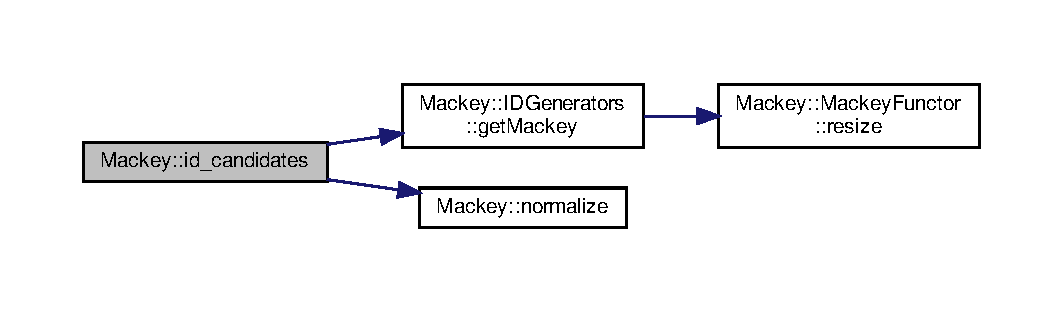
\includegraphics[width=350pt]{namespaceMackey_a83ac78e6d1695af40d0fa58af5255e84_cgraph}
\end{center}
\end{figure}
Here is the caller graph for this function\+:\nopagebreak
\begin{figure}[H]
\begin{center}
\leavevmode
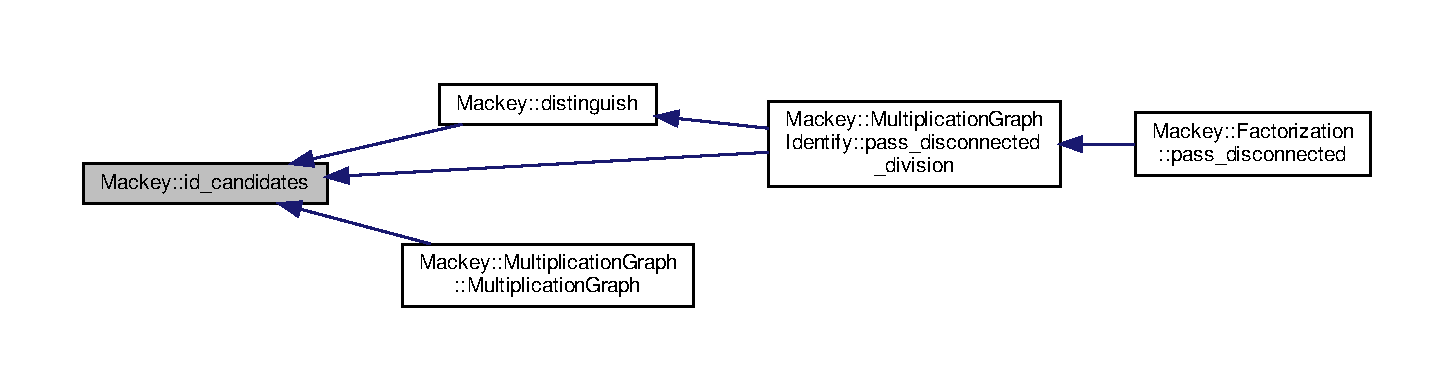
\includegraphics[width=350pt]{namespaceMackey_a83ac78e6d1695af40d0fa58af5255e84_icgraph}
\end{center}
\end{figure}
\mbox{\Hypertarget{namespaceMackey_a1ff253bf7e043ad6455b5fea23a83f09}\label{namespaceMackey_a1ff253bf7e043ad6455b5fea23a83f09}} 
\index{Mackey@{Mackey}!inSpan@{inSpan}}
\index{inSpan@{inSpan}!Mackey@{Mackey}}
\doxysubsubsection{\texorpdfstring{inSpan()}{inSpan()}}
{\footnotesize\ttfamily template$<$typename T $>$ \\
bool Mackey\+::in\+Span (\begin{DoxyParamCaption}\item[{const T \&}]{a,  }\item[{const std\+::vector$<$ T $>$ \&}]{b,  }\item[{const T \&}]{group }\end{DoxyParamCaption})}



Finds if an element is in the span of other given elements in a finitely generated abelian group. 

Here is the call graph for this function\+:\nopagebreak
\begin{figure}[H]
\begin{center}
\leavevmode
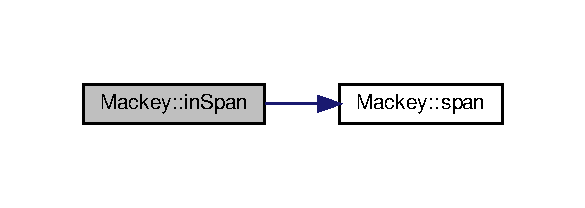
\includegraphics[width=350pt]{namespaceMackey_a1ff253bf7e043ad6455b5fea23a83f09_cgraph}
\end{center}
\end{figure}
\mbox{\Hypertarget{namespaceMackey_a4904fdc0fdcf3c23d7f3b80f59b2eafa}\label{namespaceMackey_a4904fdc0fdcf3c23d7f3b80f59b2eafa}} 
\index{Mackey@{Mackey}!intexp@{intexp}}
\index{intexp@{intexp}!Mackey@{Mackey}}
\doxysubsubsection{\texorpdfstring{intexp()}{intexp()}}
{\footnotesize\ttfamily template$<$typename T $>$ \\
T Mackey\+::intexp (\begin{DoxyParamCaption}\item[{const T}]{exponent }\end{DoxyParamCaption})\hspace{0.3cm}{\ttfamily [inline]}}



Raise power to given exponent. 

Here is the caller graph for this function\+:\nopagebreak
\begin{figure}[H]
\begin{center}
\leavevmode
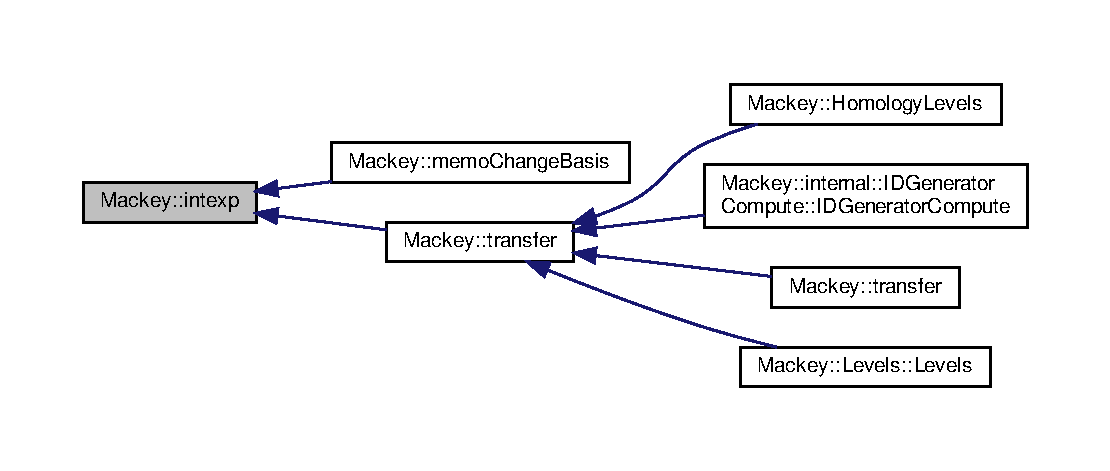
\includegraphics[width=350pt]{namespaceMackey_a4904fdc0fdcf3c23d7f3b80f59b2eafa_icgraph}
\end{center}
\end{figure}
\mbox{\Hypertarget{namespaceMackey_aa0cac9097035c5fe8448742e22e6f78b}\label{namespaceMackey_aa0cac9097035c5fe8448742e22e6f78b}} 
\index{Mackey@{Mackey}!intlog@{intlog}}
\index{intlog@{intlog}!Mackey@{Mackey}}
\doxysubsubsection{\texorpdfstring{intlog()}{intlog()}}
{\footnotesize\ttfamily template$<$typename T $>$ \\
T Mackey\+::intlog (\begin{DoxyParamCaption}\item[{const T}]{exponentiated }\end{DoxyParamCaption})\hspace{0.3cm}{\ttfamily [inline]}}



Compute log(exponentiated) with base power. 

\mbox{\Hypertarget{namespaceMackey_a8c1525b210b4699780bbe05cb16f0e7b}\label{namespaceMackey_a8c1525b210b4699780bbe05cb16f0e7b}} 
\index{Mackey@{Mackey}!inverses@{inverses}}
\index{inverses@{inverses}!Mackey@{Mackey}}
\doxysubsubsection{\texorpdfstring{inverses()}{inverses()}}
{\footnotesize\ttfamily template$<$typename T $>$ \\
std\+::vector$<$\mbox{\hyperlink{namespaceMackey_a035386035757dade630f685e508e5cf9}{mat\+\_\+t}}$<$T$>$ $>$ Mackey\+::inverses (\begin{DoxyParamCaption}\item[{const std\+::vector$<$ \mbox{\hyperlink{namespaceMackey_a035386035757dade630f685e508e5cf9}{mat\+\_\+t}}$<$ T $>$$>$ \&}]{isos,  }\item[{const T \&}]{Group }\end{DoxyParamCaption})}



Returns the inverses of all the automorphisms Group-\/$>$Group. 

Here is the call graph for this function\+:\nopagebreak
\begin{figure}[H]
\begin{center}
\leavevmode
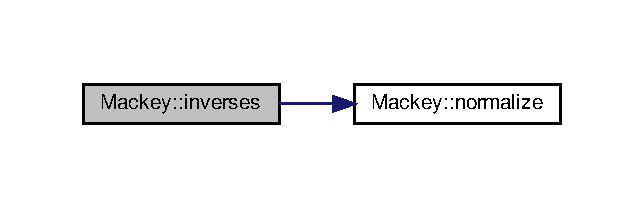
\includegraphics[width=350pt]{namespaceMackey_a8c1525b210b4699780bbe05cb16f0e7b_cgraph}
\end{center}
\end{figure}
Here is the caller graph for this function\+:\nopagebreak
\begin{figure}[H]
\begin{center}
\leavevmode
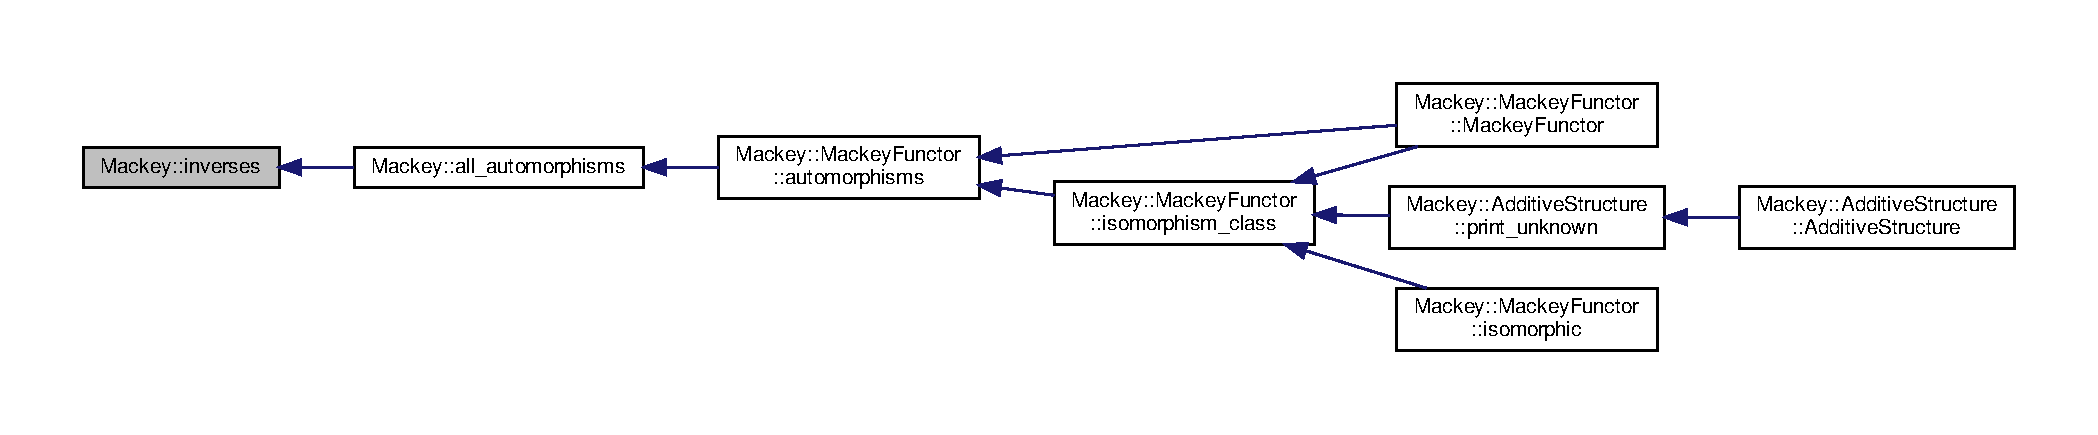
\includegraphics[width=350pt]{namespaceMackey_a8c1525b210b4699780bbe05cb16f0e7b_icgraph}
\end{center}
\end{figure}
\mbox{\Hypertarget{namespaceMackey_a011b8e23bc2eedf751a9ce7bdc9e4cb9}\label{namespaceMackey_a011b8e23bc2eedf751a9ce7bdc9e4cb9}} 
\index{Mackey@{Mackey}!invReindex@{invReindex}}
\index{invReindex@{invReindex}!Mackey@{Mackey}}
\doxysubsubsection{\texorpdfstring{invReindex()}{invReindex()}\hspace{0.1cm}{\footnotesize\ttfamily [1/2]}}
{\footnotesize\ttfamily template$<$typename T $>$ \\
int Mackey\+::inv\+Reindex (\begin{DoxyParamCaption}\item[{int}]{k,  }\item[{const T \&}]{sphere }\end{DoxyParamCaption})\hspace{0.3cm}{\ttfamily [inline]}}



Inverse of \mbox{\hyperlink{namespaceMackey_a7da73ade3ee83c4ffd614e79242d7c04}{Reindex}}. 

\mbox{\Hypertarget{namespaceMackey_a5efb3695c450e4e590b86f20700f726b}\label{namespaceMackey_a5efb3695c450e4e590b86f20700f726b}} 
\index{Mackey@{Mackey}!invReindex@{invReindex}}
\index{invReindex@{invReindex}!Mackey@{Mackey}}
\doxysubsubsection{\texorpdfstring{invReindex()}{invReindex()}\hspace{0.1cm}{\footnotesize\ttfamily [2/2]}}
{\footnotesize\ttfamily template$<$typename T $>$ \\
T Mackey\+::inv\+Reindex (\begin{DoxyParamCaption}\item[{T}]{degree }\end{DoxyParamCaption})\hspace{0.3cm}{\ttfamily [inline]}}



Inverse of \mbox{\hyperlink{namespaceMackey_a7da73ade3ee83c4ffd614e79242d7c04}{Reindex}}. 

Here is the call graph for this function\+:\nopagebreak
\begin{figure}[H]
\begin{center}
\leavevmode
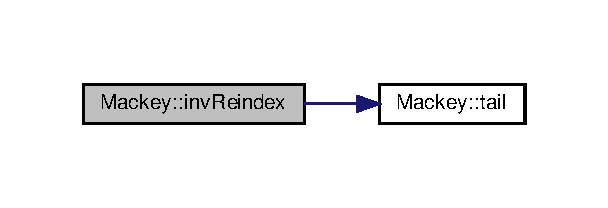
\includegraphics[width=305pt]{namespaceMackey_a5efb3695c450e4e590b86f20700f726b_cgraph}
\end{center}
\end{figure}
Here is the caller graph for this function\+:\nopagebreak
\begin{figure}[H]
\begin{center}
\leavevmode
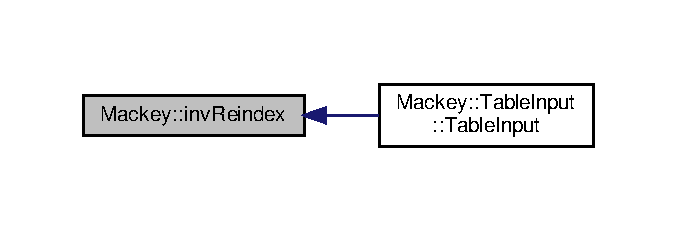
\includegraphics[width=350pt]{namespaceMackey_a5efb3695c450e4e590b86f20700f726b_icgraph}
\end{center}
\end{figure}
\mbox{\Hypertarget{namespaceMackey_a8e17fb4ada60b950c8f4efe273b23783}\label{namespaceMackey_a8e17fb4ada60b950c8f4efe273b23783}} 
\index{Mackey@{Mackey}!invRes@{invRes}}
\index{invRes@{invRes}!Mackey@{Mackey}}
\doxysubsubsection{\texorpdfstring{invRes()}{invRes()}}
{\footnotesize\ttfamily template$<$typename rank\+\_\+t , typename T $>$ \\
T Mackey\+::inv\+Res (\begin{DoxyParamCaption}\item[{const T \&}]{generator,  }\item[{const rank\+\_\+t \&}]{domain,  }\item[{const rank\+\_\+t \&}]{range }\end{DoxyParamCaption})}

The inverse of the restriction function on a generator given the ranks at the original level (domain) and the target level (range).

Recall that free \mbox{\hyperlink{namespaceMackey}{Mackey}} functors have injective restrictions, so we only need the generator to be in the image. Here is the call graph for this function\+:\nopagebreak
\begin{figure}[H]
\begin{center}
\leavevmode
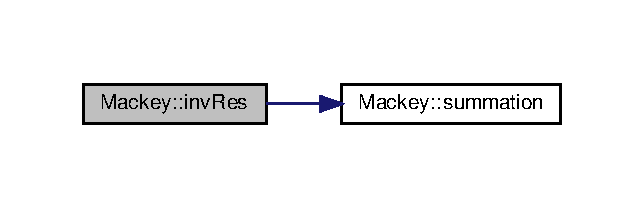
\includegraphics[width=323pt]{namespaceMackey_a8e17fb4ada60b950c8f4efe273b23783_cgraph}
\end{center}
\end{figure}
Here is the caller graph for this function\+:\nopagebreak
\begin{figure}[H]
\begin{center}
\leavevmode
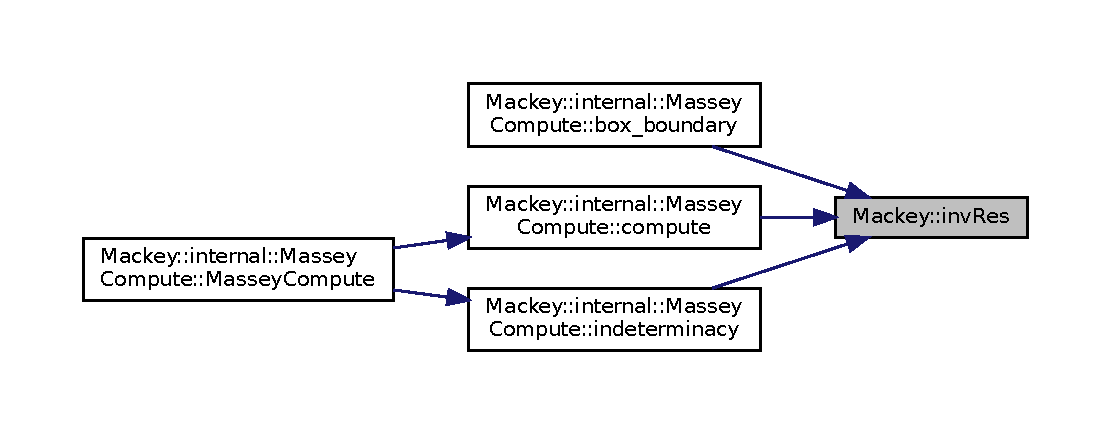
\includegraphics[width=350pt]{namespaceMackey_a8e17fb4ada60b950c8f4efe273b23783_icgraph}
\end{center}
\end{figure}
\mbox{\Hypertarget{namespaceMackey_a2b6ac22efe0be546f2c3f8abc2ceb5b7}\label{namespaceMackey_a2b6ac22efe0be546f2c3f8abc2ceb5b7}} 
\index{Mackey@{Mackey}!is\_p\_group@{is\_p\_group}}
\index{is\_p\_group@{is\_p\_group}!Mackey@{Mackey}}
\doxysubsubsection{\texorpdfstring{is\_p\_group()}{is\_p\_group()}}
{\footnotesize\ttfamily template$<$typename T $>$ \\
int Mackey\+::is\+\_\+p\+\_\+group (\begin{DoxyParamCaption}\item[{const T \&}]{Group }\end{DoxyParamCaption})}



Finds if given abelian group is actually a p-\/group and returns the p if so (otherwise returns 0) 

Here is the call graph for this function\+:\nopagebreak
\begin{figure}[H]
\begin{center}
\leavevmode
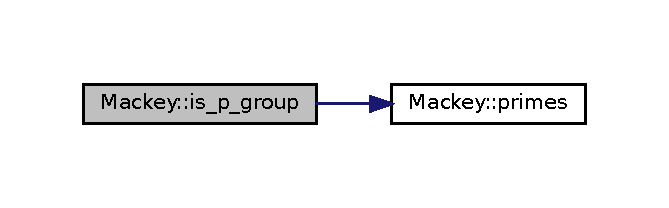
\includegraphics[width=321pt]{namespaceMackey_a2b6ac22efe0be546f2c3f8abc2ceb5b7_cgraph}
\end{center}
\end{figure}
Here is the caller graph for this function\+:\nopagebreak
\begin{figure}[H]
\begin{center}
\leavevmode
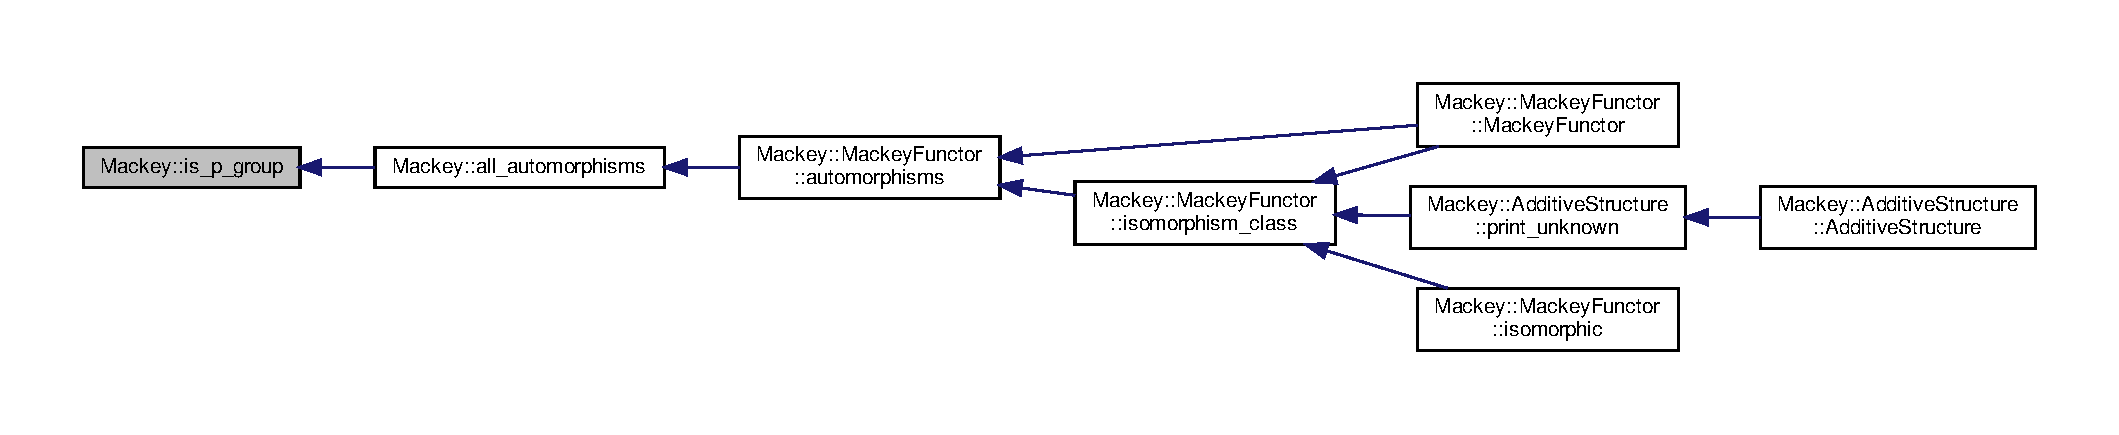
\includegraphics[width=350pt]{namespaceMackey_a2b6ac22efe0be546f2c3f8abc2ceb5b7_icgraph}
\end{center}
\end{figure}
\mbox{\Hypertarget{namespaceMackey_af70b0c547f7121b8815885dfebde67d9}\label{namespaceMackey_af70b0c547f7121b8815885dfebde67d9}} 
\index{Mackey@{Mackey}!isMultiple@{isMultiple}}
\index{isMultiple@{isMultiple}!Mackey@{Mackey}}
\doxysubsubsection{\texorpdfstring{isMultiple()}{isMultiple()}}
{\footnotesize\ttfamily template$<$typename T $>$ \\
int Mackey\+::is\+Multiple (\begin{DoxyParamCaption}\item[{const T \&}]{a,  }\item[{const T \&}]{b,  }\item[{const T \&}]{group }\end{DoxyParamCaption})}



Returns k if a=k$\ast$b in group. Returns 0 if a is not a multiple of b (so make sure a!=0) 

Here is the call graph for this function\+:\nopagebreak
\begin{figure}[H]
\begin{center}
\leavevmode
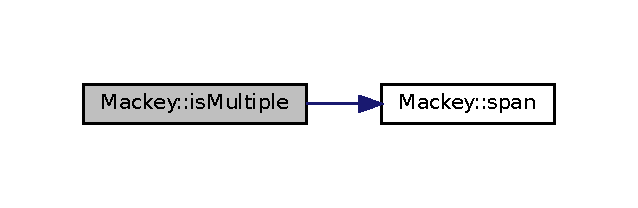
\includegraphics[width=350pt]{namespaceMackey_af70b0c547f7121b8815885dfebde67d9_cgraph}
\end{center}
\end{figure}
Here is the caller graph for this function\+:\nopagebreak
\begin{figure}[H]
\begin{center}
\leavevmode
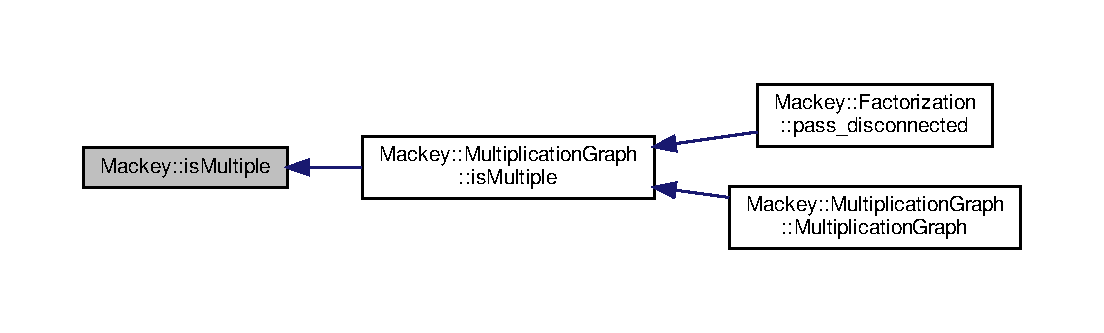
\includegraphics[width=350pt]{namespaceMackey_af70b0c547f7121b8815885dfebde67d9_icgraph}
\end{center}
\end{figure}
\mbox{\Hypertarget{namespaceMackey_a4c3647777bc890a4649ae24b138bbb79}\label{namespaceMackey_a4c3647777bc890a4649ae24b138bbb79}} 
\index{Mackey@{Mackey}!isZero@{isZero}}
\index{isZero@{isZero}!Mackey@{Mackey}}
\doxysubsubsection{\texorpdfstring{isZero()}{isZero()}}
{\footnotesize\ttfamily template$<$typename T $>$ \\
bool Mackey\+::is\+Zero (\begin{DoxyParamCaption}\item[{const std\+::vector$<$ T $>$ \&}]{a }\end{DoxyParamCaption})}



Tests if vector is zero. 

Here is the caller graph for this function\+:\nopagebreak
\begin{figure}[H]
\begin{center}
\leavevmode
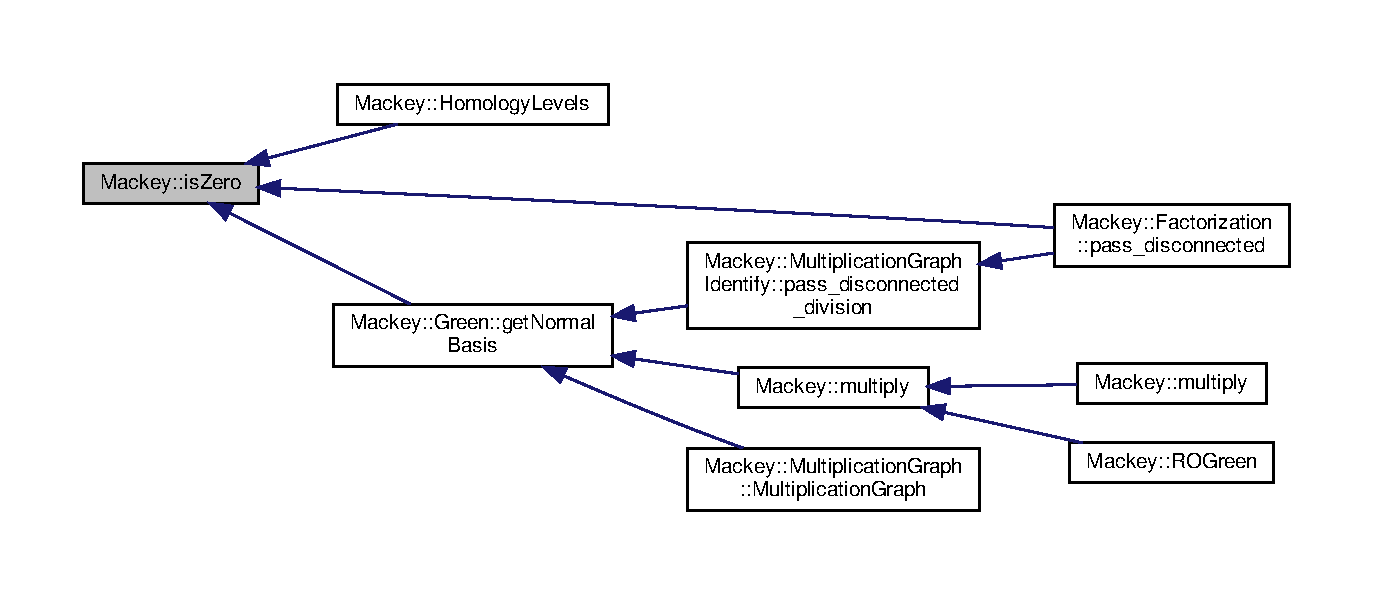
\includegraphics[width=350pt]{namespaceMackey_a4c3647777bc890a4649ae24b138bbb79_icgraph}
\end{center}
\end{figure}
\mbox{\Hypertarget{namespaceMackey_a2c0a3d97e1d5617cf9b802d0cdcfebfc}\label{namespaceMackey_a2c0a3d97e1d5617cf9b802d0cdcfebfc}} 
\index{Mackey@{Mackey}!keep\_row\_triplets@{keep\_row\_triplets}}
\index{keep\_row\_triplets@{keep\_row\_triplets}!Mackey@{Mackey}}
\doxysubsubsection{\texorpdfstring{keep\_row\_triplets()}{keep\_row\_triplets()}}
{\footnotesize\ttfamily template$<$typename T , int Storage\+Order, typename storage $>$ \\
\mbox{\hyperlink{namespaceMackey_a0b8cd52f81199d53fa1e93946d8115ef}{triplets}}$<$T, storage$>$ Mackey\+::keep\+\_\+row\+\_\+triplets (\begin{DoxyParamCaption}\item[{const Eigen\+::\+Sparse\+Matrix$<$ T, Storage\+Order, storage $>$ \&}]{a,  }\item[{const std\+::vector$<$ storage $>$ \&}]{keep }\end{DoxyParamCaption})}



Turn sparse matrix into a vector of \mbox{\hyperlink{namespaceEigen}{Eigen}} triplets. 

Here is the caller graph for this function\+:\nopagebreak
\begin{figure}[H]
\begin{center}
\leavevmode
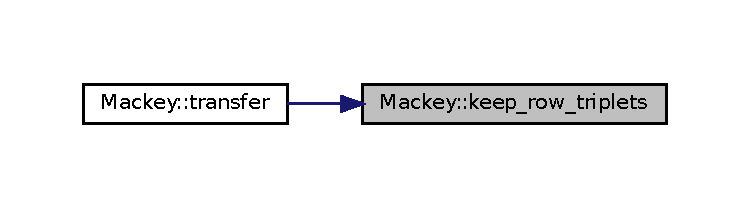
\includegraphics[width=350pt]{namespaceMackey_a2c0a3d97e1d5617cf9b802d0cdcfebfc_icgraph}
\end{center}
\end{figure}
\mbox{\Hypertarget{namespaceMackey_a9a8496759bc7bb14dcaa2284ae1d0491}\label{namespaceMackey_a9a8496759bc7bb14dcaa2284ae1d0491}} 
\index{Mackey@{Mackey}!KeepCol@{KeepCol}}
\index{KeepCol@{KeepCol}!Mackey@{Mackey}}
\doxysubsubsection{\texorpdfstring{KeepCol()}{KeepCol()}}
{\footnotesize\ttfamily template$<$typename T , typename S $>$ \\
T Mackey\+::\+Keep\+Col (\begin{DoxyParamCaption}\item[{const T \&}]{A,  }\item[{const S \&}]{Z }\end{DoxyParamCaption})}



Makes a new matrix out of A keeping only its columns indicated by \mbox{\hyperlink{classZ}{Z}}. 

Here is the caller graph for this function\+:\nopagebreak
\begin{figure}[H]
\begin{center}
\leavevmode
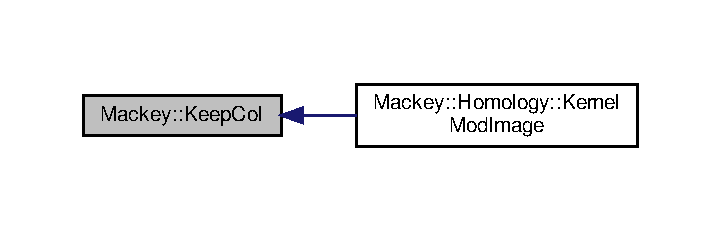
\includegraphics[width=350pt]{namespaceMackey_a9a8496759bc7bb14dcaa2284ae1d0491_icgraph}
\end{center}
\end{figure}
\mbox{\Hypertarget{namespaceMackey_ad6870101d4fd762100a3115abc4a15db}\label{namespaceMackey_ad6870101d4fd762100a3115abc4a15db}} 
\index{Mackey@{Mackey}!KeepRow@{KeepRow}}
\index{KeepRow@{KeepRow}!Mackey@{Mackey}}
\doxysubsubsection{\texorpdfstring{KeepRow()}{KeepRow()}}
{\footnotesize\ttfamily template$<$typename T , typename S $>$ \\
T Mackey\+::\+Keep\+Row (\begin{DoxyParamCaption}\item[{const T \&}]{A,  }\item[{const S \&}]{Z }\end{DoxyParamCaption})}



Makes a new matrix out of A keeping only its rows indicated by \mbox{\hyperlink{classZ}{Z}}. 

Here is the caller graph for this function\+:\nopagebreak
\begin{figure}[H]
\begin{center}
\leavevmode
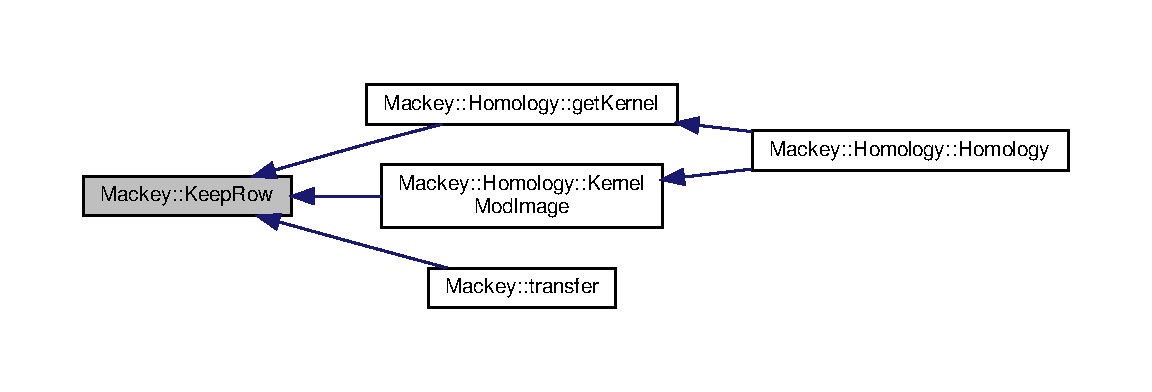
\includegraphics[width=350pt]{namespaceMackey_ad6870101d4fd762100a3115abc4a15db_icgraph}
\end{center}
\end{figure}
\mbox{\Hypertarget{namespaceMackey_a5d8ae76ffb9440e27bfca124d26ee1b2}\label{namespaceMackey_a5d8ae76ffb9440e27bfca124d26ee1b2}} 
\index{Mackey@{Mackey}!lcm@{lcm}}
\index{lcm@{lcm}!Mackey@{Mackey}}
\doxysubsubsection{\texorpdfstring{lcm()}{lcm()}}
{\footnotesize\ttfamily template$<$typename T $>$ \\
int Mackey\+::lcm (\begin{DoxyParamCaption}\item[{const T \&}]{v }\end{DoxyParamCaption})}



Least common multiple of vector of elements. 

Here is the caller graph for this function\+:\nopagebreak
\begin{figure}[H]
\begin{center}
\leavevmode
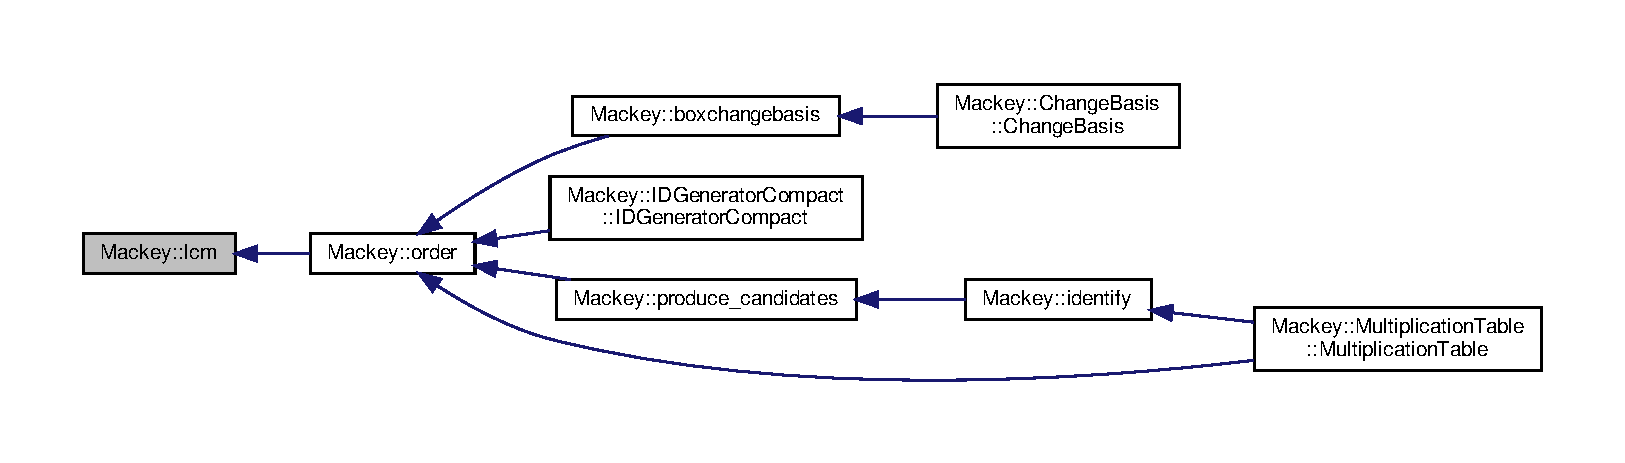
\includegraphics[width=350pt]{namespaceMackey_a5d8ae76ffb9440e27bfca124d26ee1b2_icgraph}
\end{center}
\end{figure}
\mbox{\Hypertarget{namespaceMackey_ac34d89121229145967593a1b6c30d7aa}\label{namespaceMackey_ac34d89121229145967593a1b6c30d7aa}} 
\index{Mackey@{Mackey}!load@{load}}
\index{load@{load}!Mackey@{Mackey}}
\doxysubsubsection{\texorpdfstring{load()}{load()}}
{\footnotesize\ttfamily template$<$typename Archive , typename rank\+\_\+t , typename diff\+\_\+t $>$ \\
void Mackey\+::load (\begin{DoxyParamCaption}\item[{Archive \&}]{archive,  }\item[{\mbox{\hyperlink{classMackey_1_1MultiplicationTable}{Multiplication\+Table}}$<$ rank\+\_\+t, diff\+\_\+t $>$ \&}]{M }\end{DoxyParamCaption})}



\mbox{\hyperlink{classMackey_1_1MultiplicationTable}{Multiplication\+Table}} cerealize. 

\mbox{\Hypertarget{namespaceMackey_a735958355cdca12e0d312b7e604f28bc}\label{namespaceMackey_a735958355cdca12e0d312b7e604f28bc}} 
\index{Mackey@{Mackey}!loader@{loader}}
\index{loader@{loader}!Mackey@{Mackey}}
\doxysubsubsection{\texorpdfstring{loader()}{loader()}}
{\footnotesize\ttfamily template$<$typename T $>$ \\
void Mackey\+::loader (\begin{DoxyParamCaption}\item[{T \&}]{A,  }\item[{const std\+::string \&}]{filename,  }\item[{const std\+::string \&}]{type }\end{DoxyParamCaption})}



Loads object from binary file of given name. Serialization is provided by cereal. 

\mbox{\Hypertarget{namespaceMackey_a114f8d4069f6e5964f07c2fec3bdc9b7}\label{namespaceMackey_a114f8d4069f6e5964f07c2fec3bdc9b7}} 
\index{Mackey@{Mackey}!make\_triplets@{make\_triplets}}
\index{make\_triplets@{make\_triplets}!Mackey@{Mackey}}
\doxysubsubsection{\texorpdfstring{make\_triplets()}{make\_triplets()}}
{\footnotesize\ttfamily template$<$typename T , int Storage\+Order, typename storage $>$ \\
\mbox{\hyperlink{namespaceMackey_a0b8cd52f81199d53fa1e93946d8115ef}{triplets}}$<$T, storage$>$ Mackey\+::make\+\_\+triplets (\begin{DoxyParamCaption}\item[{const Eigen\+::\+Sparse\+Matrix$<$ T, Storage\+Order, storage $>$ \&}]{a }\end{DoxyParamCaption})}



Turn sparse matrix into a vector of \mbox{\hyperlink{namespaceEigen}{Eigen}} triplets. 

\mbox{\Hypertarget{namespaceMackey_a1c34295db9666bc7e86b2972c345d291}\label{namespaceMackey_a1c34295db9666bc7e86b2972c345d291}} 
\index{Mackey@{Mackey}!MatrixMixer@{MatrixMixer}}
\index{MatrixMixer@{MatrixMixer}!Mackey@{Mackey}}
\doxysubsubsection{\texorpdfstring{MatrixMixer()}{MatrixMixer()}}
{\footnotesize\ttfamily template$<$typename T $>$ \\
T Mackey\+::\+Matrix\+Mixer (\begin{DoxyParamCaption}\item[{std\+::vector$<$ T $>$ \&}]{L,  }\item[{std\+::vector$<$ T $>$ \&}]{R,  }\item[{int}]{rows,  }\item[{int}]{cols }\end{DoxyParamCaption})}



Mixes the left and right differentials to produce the differential for the box product. 

The left differentials are stored in a vector L and the right differentials in a vector R. The mixing is L\mbox{[}0\mbox{]}, then R\mbox{[}0\mbox{]} directly to the right, then L\mbox{[}1\mbox{]} directly below then... It\textquotesingle{}s assumed that L,R have consistent dimensions for the blocks to fit coherently. \mbox{\Hypertarget{namespaceMackey_a257bcf5aabab2d73fdb13a23cb975d93}\label{namespaceMackey_a257bcf5aabab2d73fdb13a23cb975d93}} 
\index{Mackey@{Mackey}!mod\_normalize@{mod\_normalize}}
\index{mod\_normalize@{mod\_normalize}!Mackey@{Mackey}}
\doxysubsubsection{\texorpdfstring{mod\_normalize()}{mod\_normalize()}}
{\footnotesize\ttfamily template$<$typename T $>$ \\
void Mackey\+::mod\+\_\+normalize (\begin{DoxyParamCaption}\item[{T \&}]{element,  }\item[{const T \&}]{group }\end{DoxyParamCaption})}



Normalizes the element in a group so that 0$<$=element\mbox{[}i\mbox{]}$<$=group\mbox{[}i\mbox{]} if group\mbox{[}i\mbox{]}!=1. 

Here is the caller graph for this function\+:\nopagebreak
\begin{figure}[H]
\begin{center}
\leavevmode
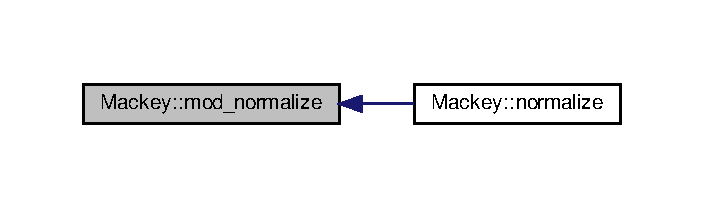
\includegraphics[width=350pt]{namespaceMackey_a257bcf5aabab2d73fdb13a23cb975d93_icgraph}
\end{center}
\end{figure}
\mbox{\Hypertarget{namespaceMackey_a2eca4cc709501ad3fc20b82fe4bcbd33}\label{namespaceMackey_a2eca4cc709501ad3fc20b82fe4bcbd33}} 
\index{Mackey@{Mackey}!multiply@{multiply}}
\index{multiply@{multiply}!Mackey@{Mackey}}
\doxysubsubsection{\texorpdfstring{multiply()}{multiply()}\hspace{0.1cm}{\footnotesize\ttfamily [1/2]}}
{\footnotesize\ttfamily template$<$typename rank\+\_\+t , typename diff\+\_\+t $>$ \\
rank\+\_\+t Mackey\+::multiply (\begin{DoxyParamCaption}\item[{const \mbox{\hyperlink{classMackey_1_1Chains}{Chains}}$<$ rank\+\_\+t, diff\+\_\+t $>$ \&}]{C,  }\item[{const \mbox{\hyperlink{classMackey_1_1Chains}{Chains}}$<$ rank\+\_\+t, diff\+\_\+t $>$ \&}]{D,  }\item[{int}]{level,  }\item[{int}]{degreeC,  }\item[{int}]{degreeD }\end{DoxyParamCaption})}

Here is the call graph for this function\+:\nopagebreak
\begin{figure}[H]
\begin{center}
\leavevmode
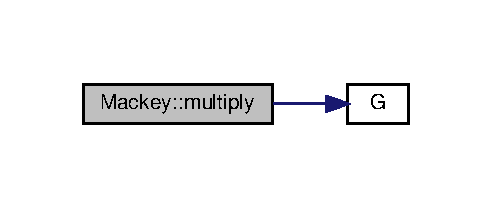
\includegraphics[width=350pt]{namespaceMackey_a2eca4cc709501ad3fc20b82fe4bcbd33_cgraph}
\end{center}
\end{figure}
\mbox{\Hypertarget{namespaceMackey_a80dbde3a859378ede596b48869ec50d9}\label{namespaceMackey_a80dbde3a859378ede596b48869ec50d9}} 
\index{Mackey@{Mackey}!multiply@{multiply}}
\index{multiply@{multiply}!Mackey@{Mackey}}
\doxysubsubsection{\texorpdfstring{multiply()}{multiply()}\hspace{0.1cm}{\footnotesize\ttfamily [2/2]}}
{\footnotesize\ttfamily template$<$typename rank\+\_\+t , typename diff\+\_\+t $>$ \\
rank\+\_\+t Mackey\+::multiply (\begin{DoxyParamCaption}\item[{const \mbox{\hyperlink{classMackey_1_1Chains}{Chains}}$<$ rank\+\_\+t, diff\+\_\+t $>$ \&}]{C,  }\item[{const \mbox{\hyperlink{classMackey_1_1Chains}{Chains}}$<$ rank\+\_\+t, diff\+\_\+t $>$ \&}]{D,  }\item[{int}]{level,  }\item[{int}]{degreeC,  }\item[{int}]{degreeD,  }\item[{int}]{selectC,  }\item[{int}]{selectD }\end{DoxyParamCaption})}

Here is the call graph for this function\+:\nopagebreak
\begin{figure}[H]
\begin{center}
\leavevmode
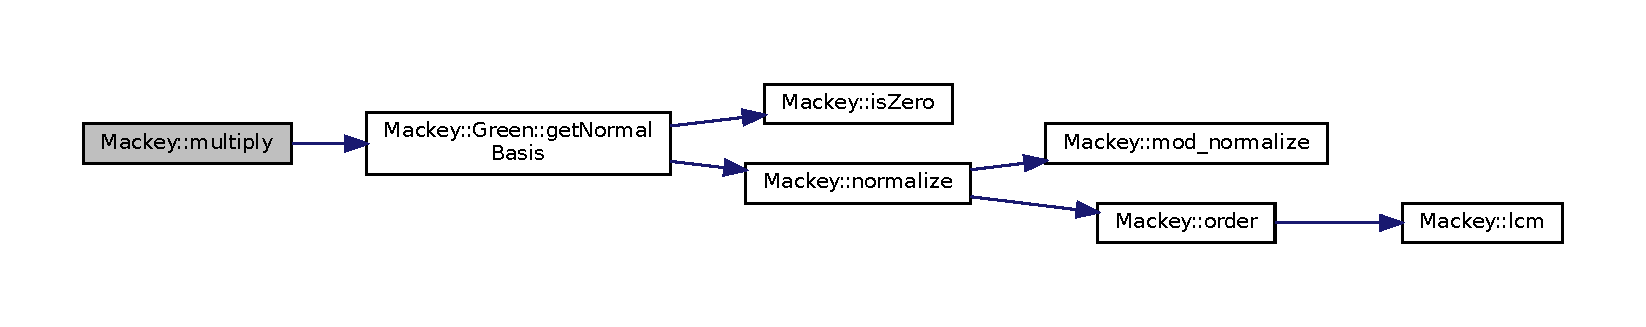
\includegraphics[width=350pt]{namespaceMackey_a80dbde3a859378ede596b48869ec50d9_cgraph}
\end{center}
\end{figure}
Here is the caller graph for this function\+:\nopagebreak
\begin{figure}[H]
\begin{center}
\leavevmode
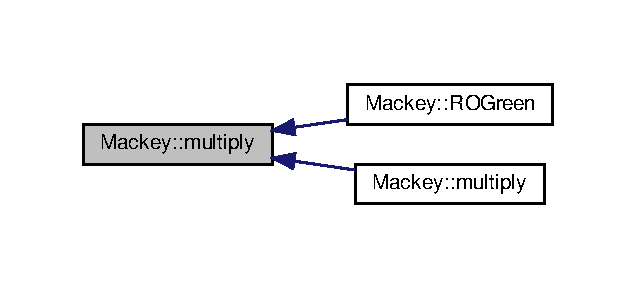
\includegraphics[width=319pt]{namespaceMackey_a80dbde3a859378ede596b48869ec50d9_icgraph}
\end{center}
\end{figure}
\mbox{\Hypertarget{namespaceMackey_a5ae32d04bca298d2d8735635ae45b971}\label{namespaceMackey_a5ae32d04bca298d2d8735635ae45b971}} 
\index{Mackey@{Mackey}!normalize@{normalize}}
\index{normalize@{normalize}!Mackey@{Mackey}}
\doxysubsubsection{\texorpdfstring{normalize()}{normalize()}\hspace{0.1cm}{\footnotesize\ttfamily [1/2]}}
{\footnotesize\ttfamily template$<$typename T , typename S $>$ \\
void Mackey\+::normalize (\begin{DoxyParamCaption}\item[{Eigen\+::\+Matrix$<$ T, -\/1, -\/1 $>$ \&}]{linmap,  }\item[{const Eigen\+::\+Matrix$<$ S, 1, -\/1 $>$ \&}]{range }\end{DoxyParamCaption})}



Normalize linear map if the range is finitely generated abelian (reduce n in Z/n to 0 etc.). 

\mbox{\Hypertarget{namespaceMackey_a635c87980358b97256fe159f0c59bb80}\label{namespaceMackey_a635c87980358b97256fe159f0c59bb80}} 
\index{Mackey@{Mackey}!normalize@{normalize}}
\index{normalize@{normalize}!Mackey@{Mackey}}
\doxysubsubsection{\texorpdfstring{normalize()}{normalize()}\hspace{0.1cm}{\footnotesize\ttfamily [2/2]}}
{\footnotesize\ttfamily template$<$typename T $>$ \\
void Mackey\+::normalize (\begin{DoxyParamCaption}\item[{Eigen\+::\+Matrix$<$ T, 1,-\/1 $>$ \&}]{element,  }\item[{const Eigen\+::\+Matrix$<$ T, 1, -\/1 $>$ \&}]{group }\end{DoxyParamCaption})}



Normalizes the element in a group to have minimal signs amongst its multiples. 

Here is the call graph for this function\+:\nopagebreak
\begin{figure}[H]
\begin{center}
\leavevmode
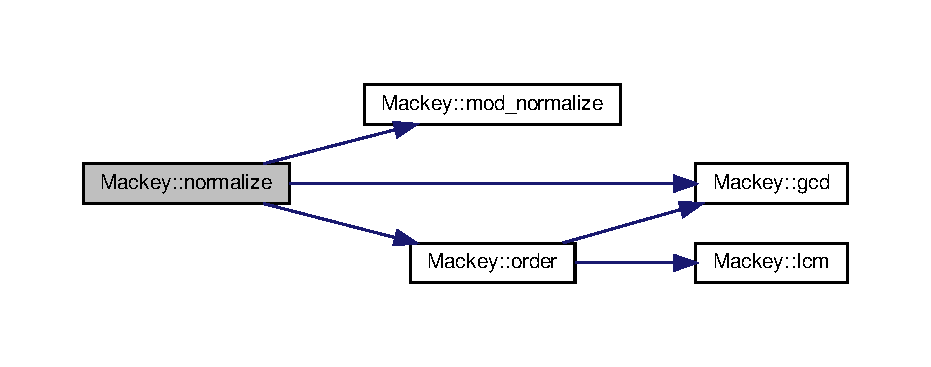
\includegraphics[width=350pt]{namespaceMackey_a635c87980358b97256fe159f0c59bb80_cgraph}
\end{center}
\end{figure}
Here is the caller graph for this function\+:\nopagebreak
\begin{figure}[H]
\begin{center}
\leavevmode
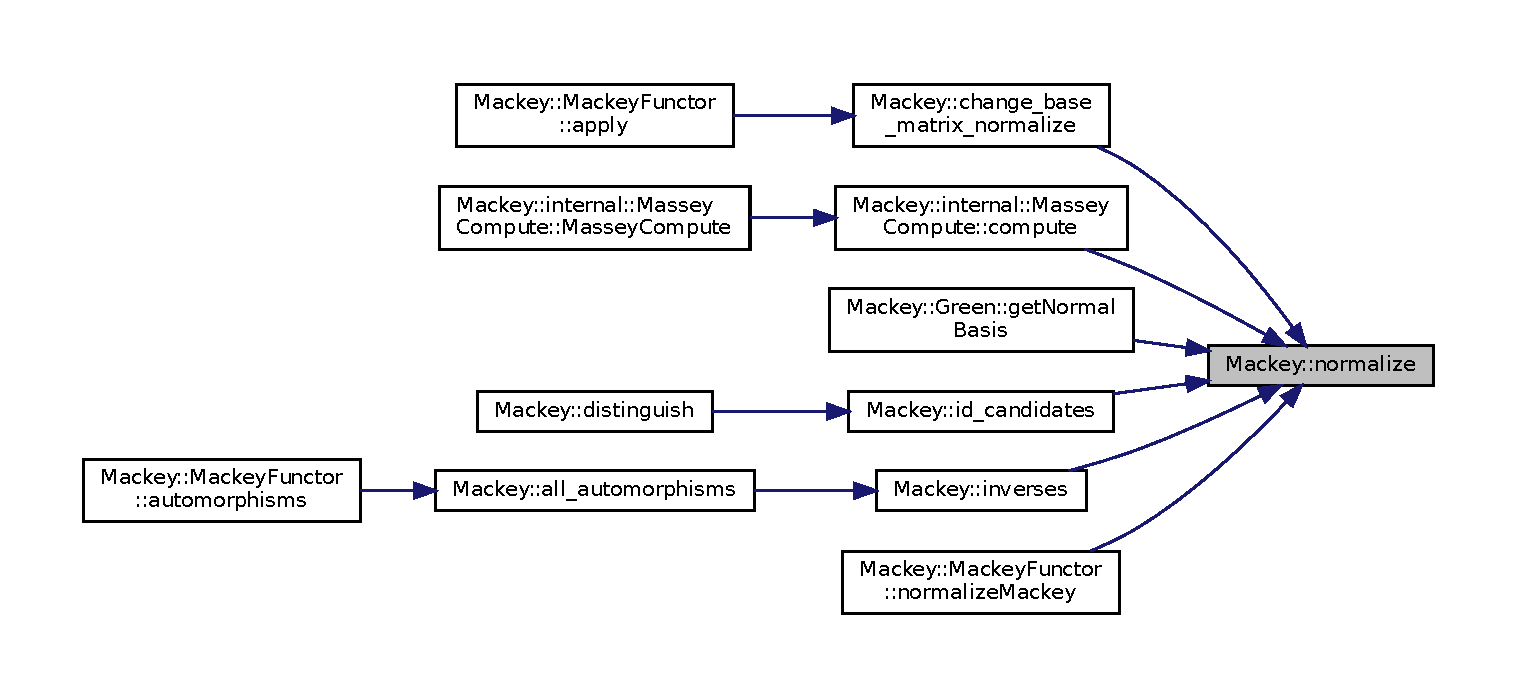
\includegraphics[width=350pt]{namespaceMackey_a635c87980358b97256fe159f0c59bb80_icgraph}
\end{center}
\end{figure}
\mbox{\Hypertarget{namespaceMackey_a463bb762b4edc2f283e8d1c0c466aedf}\label{namespaceMackey_a463bb762b4edc2f283e8d1c0c466aedf}} 
\index{Mackey@{Mackey}!normalize\_minus@{normalize\_minus}}
\index{normalize\_minus@{normalize\_minus}!Mackey@{Mackey}}
\doxysubsubsection{\texorpdfstring{normalize\_minus()}{normalize\_minus()}}
{\footnotesize\ttfamily template$<$typename Scalar $>$ \\
void Mackey\+::normalize\+\_\+minus (\begin{DoxyParamCaption}\item[{Eigen\+::\+Matrix$<$ Scalar, -\/1, -\/1 $>$ \&}]{linmap,  }\item[{const Eigen\+::\+Matrix$<$ Scalar, 1, -\/1 $>$ \&}]{range,  }\item[{bool}]{positive }\end{DoxyParamCaption})}



Normalize linear map if the range is finitely generated abelian (reduce n in Z/n to 0 etc.) allowing negative entries. 

Here is the caller graph for this function\+:\nopagebreak
\begin{figure}[H]
\begin{center}
\leavevmode
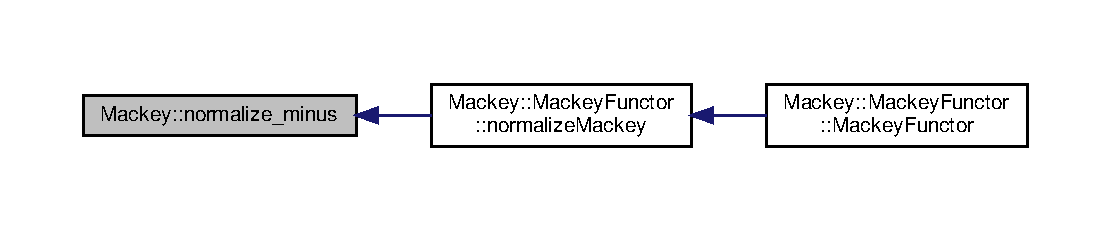
\includegraphics[width=350pt]{namespaceMackey_a463bb762b4edc2f283e8d1c0c466aedf_icgraph}
\end{center}
\end{figure}
\mbox{\Hypertarget{namespaceMackey_ae235ee5dd92dc1ca64388b8fbb1b4d75}\label{namespaceMackey_ae235ee5dd92dc1ca64388b8fbb1b4d75}} 
\index{Mackey@{Mackey}!operator$\ast$@{operator$\ast$}}
\index{operator$\ast$@{operator$\ast$}!Mackey@{Mackey}}
\doxysubsubsection{\texorpdfstring{operator$\ast$()}{operator*()}}
{\footnotesize\ttfamily template$<$typename T $>$ \\
std\+::vector$<$T$>$ Mackey\+::operator$\ast$ (\begin{DoxyParamCaption}\item[{T}]{a,  }\item[{const std\+::vector$<$ T $>$ \&}]{b }\end{DoxyParamCaption})}



Product of element and vector. 

\mbox{\Hypertarget{namespaceMackey_a738f2b46b7d0c37be203a17083801bbd}\label{namespaceMackey_a738f2b46b7d0c37be203a17083801bbd}} 
\index{Mackey@{Mackey}!operator+@{operator+}}
\index{operator+@{operator+}!Mackey@{Mackey}}
\doxysubsubsection{\texorpdfstring{operator+()}{operator+()}\hspace{0.1cm}{\footnotesize\ttfamily [1/2]}}
{\footnotesize\ttfamily template$<$typename rank\+\_\+t $>$ \\
\mbox{\hyperlink{classMackey_1_1MackeyFunctor}{Mackey\+Functor}}$<$rank\+\_\+t$>$ Mackey\+::operator+ (\begin{DoxyParamCaption}\item[{const \mbox{\hyperlink{classMackey_1_1MackeyFunctor}{Mackey\+Functor}}$<$ rank\+\_\+t $>$ \&}]{M,  }\item[{const \mbox{\hyperlink{classMackey_1_1MackeyFunctor}{Mackey\+Functor}}$<$ rank\+\_\+t $>$ \&}]{N }\end{DoxyParamCaption})}



The sum of two \mbox{\hyperlink{namespaceMackey}{Mackey}} functors. 

Here is the call graph for this function\+:\nopagebreak
\begin{figure}[H]
\begin{center}
\leavevmode
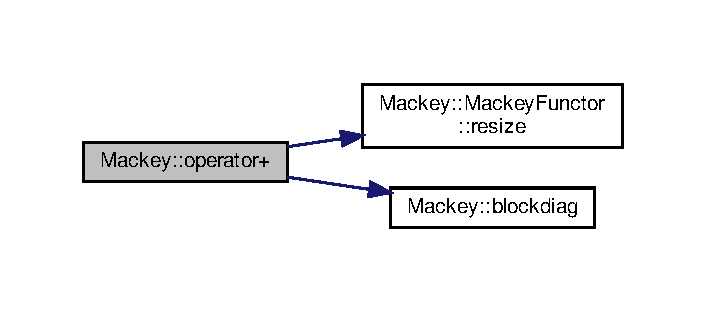
\includegraphics[width=350pt]{namespaceMackey_a738f2b46b7d0c37be203a17083801bbd_cgraph}
\end{center}
\end{figure}
\mbox{\Hypertarget{namespaceMackey_adb4974b5ffe533abb955ccb6b9096155}\label{namespaceMackey_adb4974b5ffe533abb955ccb6b9096155}} 
\index{Mackey@{Mackey}!operator+@{operator+}}
\index{operator+@{operator+}!Mackey@{Mackey}}
\doxysubsubsection{\texorpdfstring{operator+()}{operator+()}\hspace{0.1cm}{\footnotesize\ttfamily [2/2]}}
{\footnotesize\ttfamily template$<$typename T $>$ \\
std\+::vector$<$T$>$ Mackey\+::operator+ (\begin{DoxyParamCaption}\item[{const std\+::vector$<$ T $>$ \&}]{a,  }\item[{const std\+::vector$<$ T $>$ \&}]{b }\end{DoxyParamCaption})}



Coordinate-\/wise sum of vectors (up to the minimum of their lengths) 

\mbox{\Hypertarget{namespaceMackey_a9d67cfe3e93ac3ef2301547372b48e15}\label{namespaceMackey_a9d67cfe3e93ac3ef2301547372b48e15}} 
\index{Mackey@{Mackey}!operator-\/@{operator-\/}}
\index{operator-\/@{operator-\/}!Mackey@{Mackey}}
\doxysubsubsection{\texorpdfstring{operator-\/()}{operator-()}\hspace{0.1cm}{\footnotesize\ttfamily [1/2]}}
{\footnotesize\ttfamily template$<$typename T $>$ \\
std\+::vector$<$T$>$ Mackey\+::operator-\/ (\begin{DoxyParamCaption}\item[{const std\+::vector$<$ T $>$ \&}]{a }\end{DoxyParamCaption})}



Coordinate-\/wise opposite of vector. 

\mbox{\Hypertarget{namespaceMackey_ae86e49097ef9a09ebcd0173881e88786}\label{namespaceMackey_ae86e49097ef9a09ebcd0173881e88786}} 
\index{Mackey@{Mackey}!operator-\/@{operator-\/}}
\index{operator-\/@{operator-\/}!Mackey@{Mackey}}
\doxysubsubsection{\texorpdfstring{operator-\/()}{operator-()}\hspace{0.1cm}{\footnotesize\ttfamily [2/2]}}
{\footnotesize\ttfamily template$<$typename T $>$ \\
std\+::vector$<$T$>$ Mackey\+::operator-\/ (\begin{DoxyParamCaption}\item[{const std\+::vector$<$ T $>$ \&}]{a,  }\item[{const std\+::vector$<$ T $>$ \&}]{b }\end{DoxyParamCaption})}



Coordinate-\/wise difference of vectors (up to the minimum of their lengths) 

\mbox{\Hypertarget{namespaceMackey_a28ea49d917fa3784b3fb529932e2fede}\label{namespaceMackey_a28ea49d917fa3784b3fb529932e2fede}} 
\index{Mackey@{Mackey}!operator$<$$<$@{operator$<$$<$}}
\index{operator$<$$<$@{operator$<$$<$}!Mackey@{Mackey}}
\doxysubsubsection{\texorpdfstring{operator$<$$<$()}{operator<<()}\hspace{0.1cm}{\footnotesize\ttfamily [1/6]}}
{\footnotesize\ttfamily template$<$typename graph\+\_\+t , typename node\+\_\+names\+\_\+t $>$ \\
std\+::enable\+\_\+if\+\_\+t$<$\mbox{\hyperlink{structMackey_1_1SFINAE_a8d7c08b95cd45987c1494510c7879f72}{S\+F\+I\+N\+A\+E\+::is\+\_\+graph\+\_\+t}}$<$graph\+\_\+t$>$\+::value, \mbox{\hyperlink{structMackey_1_1GraphPrinter}{Graph\+Printer}}$<$graph\+\_\+t, node\+\_\+names\+\_\+t$>$ $>$ Mackey\+::operator$<$$<$ (\begin{DoxyParamCaption}\item[{const graph\+\_\+t \&}]{G,  }\item[{const node\+\_\+names\+\_\+t \&}]{node\+\_\+names }\end{DoxyParamCaption})}



Adjoins node names to graph to get it ready for printing. 

Here is the call graph for this function\+:\nopagebreak
\begin{figure}[H]
\begin{center}
\leavevmode
\includegraphics[width=350pt]{namespaceMackey_a28ea49d917fa3784b3fb529932e2fede_cgraph}
\end{center}
\end{figure}
\mbox{\Hypertarget{namespaceMackey_a4459d62150c04a8a525c5cac50a25618}\label{namespaceMackey_a4459d62150c04a8a525c5cac50a25618}} 
\index{Mackey@{Mackey}!operator$<$$<$@{operator$<$$<$}}
\index{operator$<$$<$@{operator$<$$<$}!Mackey@{Mackey}}
\doxysubsubsection{\texorpdfstring{operator$<$$<$()}{operator<<()}\hspace{0.1cm}{\footnotesize\ttfamily [2/6]}}
{\footnotesize\ttfamily template$<$typename rank\+\_\+t , typename diff\+\_\+t $>$ \\
std\+::ostream\& Mackey\+::operator$<$$<$ (\begin{DoxyParamCaption}\item[{std\+::ostream \&}]{os,  }\item[{const \mbox{\hyperlink{classMackey_1_1FactorizationPrinter}{Factorization\+Printer}}$<$ rank\+\_\+t, diff\+\_\+t $>$ \&}]{F }\end{DoxyParamCaption})}



Prints \mbox{\hyperlink{classMackey_1_1Factorization}{Factorization}}. 

Here is the call graph for this function\+:\nopagebreak
\begin{figure}[H]
\begin{center}
\leavevmode
\includegraphics[width=350pt]{namespaceMackey_a4459d62150c04a8a525c5cac50a25618_cgraph}
\end{center}
\end{figure}
\mbox{\Hypertarget{namespaceMackey_ade9d5fa2d9183c796bb3a6b7302c58e5}\label{namespaceMackey_ade9d5fa2d9183c796bb3a6b7302c58e5}} 
\index{Mackey@{Mackey}!operator$<$$<$@{operator$<$$<$}}
\index{operator$<$$<$@{operator$<$$<$}!Mackey@{Mackey}}
\doxysubsubsection{\texorpdfstring{operator$<$$<$()}{operator<<()}\hspace{0.1cm}{\footnotesize\ttfamily [3/6]}}
{\footnotesize\ttfamily template$<$typename graph\+\_\+t $>$ \\
std\+::enable\+\_\+if\+\_\+t$<$\mbox{\hyperlink{structMackey_1_1SFINAE_a8d7c08b95cd45987c1494510c7879f72}{S\+F\+I\+N\+A\+E\+::is\+\_\+graph\+\_\+t}}$<$graph\+\_\+t$>$\+::value, std\+::ostream\&$>$ Mackey\+::operator$<$$<$ (\begin{DoxyParamCaption}\item[{std\+::ostream \&}]{os,  }\item[{const graph\+\_\+t \&}]{G }\end{DoxyParamCaption})}



Prints the graph in .dot format with unnamed nodes. 

\mbox{\Hypertarget{namespaceMackey_a27403feca74a3b3619339323e2a8b186}\label{namespaceMackey_a27403feca74a3b3619339323e2a8b186}} 
\index{Mackey@{Mackey}!operator$<$$<$@{operator$<$$<$}}
\index{operator$<$$<$@{operator$<$$<$}!Mackey@{Mackey}}
\doxysubsubsection{\texorpdfstring{operator$<$$<$()}{operator<<()}\hspace{0.1cm}{\footnotesize\ttfamily [4/6]}}
{\footnotesize\ttfamily template$<$typename graph\+\_\+t , typename node\+\_\+names\+\_\+t $>$ \\
std\+::ostream\& Mackey\+::operator$<$$<$ (\begin{DoxyParamCaption}\item[{std\+::ostream \&}]{os,  }\item[{const \mbox{\hyperlink{structMackey_1_1GraphPrinter}{Graph\+Printer}}$<$ graph\+\_\+t, node\+\_\+names\+\_\+t $>$ \&}]{GP }\end{DoxyParamCaption})}



Prints graph in .dot format with named nodes if provided. 

\mbox{\Hypertarget{namespaceMackey_aaf9e6d978fdb55a757223964390b2fc0}\label{namespaceMackey_aaf9e6d978fdb55a757223964390b2fc0}} 
\index{Mackey@{Mackey}!operator$<$$<$@{operator$<$$<$}}
\index{operator$<$$<$@{operator$<$$<$}!Mackey@{Mackey}}
\doxysubsubsection{\texorpdfstring{operator$<$$<$()}{operator<<()}\hspace{0.1cm}{\footnotesize\ttfamily [5/6]}}
{\footnotesize\ttfamily template$<$typename rank\+\_\+t $>$ \\
std\+::ostream\& Mackey\+::operator$<$$<$ (\begin{DoxyParamCaption}\item[{std\+::ostream \&}]{out,  }\item[{const \mbox{\hyperlink{classMackey_1_1MackeyFunctor}{Mackey\+Functor}}$<$ rank\+\_\+t $>$ \&}]{M }\end{DoxyParamCaption})}

Here is the call graph for this function\+:\nopagebreak
\begin{figure}[H]
\begin{center}
\leavevmode
\includegraphics[width=350pt]{namespaceMackey_aaf9e6d978fdb55a757223964390b2fc0_cgraph}
\end{center}
\end{figure}
\mbox{\Hypertarget{namespaceMackey_aa4da3e3b46b9cb20f3be57d7e5da2d5d}\label{namespaceMackey_aa4da3e3b46b9cb20f3be57d7e5da2d5d}} 
\index{Mackey@{Mackey}!operator$<$$<$@{operator$<$$<$}}
\index{operator$<$$<$@{operator$<$$<$}!Mackey@{Mackey}}
\doxysubsubsection{\texorpdfstring{operator$<$$<$()}{operator<<()}\hspace{0.1cm}{\footnotesize\ttfamily [6/6]}}
{\footnotesize\ttfamily template$<$typename T $>$ \\
std\+::ostream\& Mackey\+::operator$<$$<$ (\begin{DoxyParamCaption}\item[{std\+::ostream \&}]{out,  }\item[{const std\+::vector$<$ T $>$ \&}]{a }\end{DoxyParamCaption})}



Printing a vector. 

\mbox{\Hypertarget{namespaceMackey_a2c0afbb179b17f9c32cf6d982ff6cb67}\label{namespaceMackey_a2c0afbb179b17f9c32cf6d982ff6cb67}} 
\index{Mackey@{Mackey}!operator==@{operator==}}
\index{operator==@{operator==}!Mackey@{Mackey}}
\doxysubsubsection{\texorpdfstring{operator==()}{operator==()}\hspace{0.1cm}{\footnotesize\ttfamily [1/2]}}
{\footnotesize\ttfamily template$<$typename rank\+\_\+t , typename diff\+\_\+t $>$ \\
bool Mackey\+::operator== (\begin{DoxyParamCaption}\item[{const \mbox{\hyperlink{classMackey_1_1Green}{Green}}$<$ rank\+\_\+t, diff\+\_\+t $>$ \&}]{G,  }\item[{const \mbox{\hyperlink{classMackey_1_1Green}{Green}}$<$ rank\+\_\+t, diff\+\_\+t $>$ \&}]{H }\end{DoxyParamCaption})}

\mbox{\Hypertarget{namespaceMackey_a1e45f568bb1a05dba7cc9eafb6fd3321}\label{namespaceMackey_a1e45f568bb1a05dba7cc9eafb6fd3321}} 
\index{Mackey@{Mackey}!operator==@{operator==}}
\index{operator==@{operator==}!Mackey@{Mackey}}
\doxysubsubsection{\texorpdfstring{operator==()}{operator==()}\hspace{0.1cm}{\footnotesize\ttfamily [2/2]}}
{\footnotesize\ttfamily template$<$typename rank\+\_\+t $>$ \\
bool Mackey\+::operator== (\begin{DoxyParamCaption}\item[{const \mbox{\hyperlink{classMackey_1_1IDGenerators}{I\+D\+Generators}}$<$ rank\+\_\+t $>$ \&}]{I,  }\item[{const \mbox{\hyperlink{classMackey_1_1IDGenerators}{I\+D\+Generators}}$<$ rank\+\_\+t $>$ \&}]{J }\end{DoxyParamCaption})}

\mbox{\Hypertarget{namespaceMackey_a4abdca157edcf425b1e7ceff39d74c2f}\label{namespaceMackey_a4abdca157edcf425b1e7ceff39d74c2f}} 
\index{Mackey@{Mackey}!order@{order}}
\index{order@{order}!Mackey@{Mackey}}
\doxysubsubsection{\texorpdfstring{order()}{order()}}
{\footnotesize\ttfamily template$<$typename T , typename S $>$ \\
int Mackey\+::order (\begin{DoxyParamCaption}\item[{const T \&}]{element,  }\item[{const S \&}]{group }\end{DoxyParamCaption})}



Finds the order of element in given finitely generated abelian group. Returns 0 if order is infinite. 

T,S are vectors or 1d \mbox{\hyperlink{namespaceEigen}{Eigen}} matrices Here is the call graph for this function\+:\nopagebreak
\begin{figure}[H]
\begin{center}
\leavevmode
\includegraphics[width=278pt]{namespaceMackey_a4abdca157edcf425b1e7ceff39d74c2f_cgraph}
\end{center}
\end{figure}
Here is the caller graph for this function\+:\nopagebreak
\begin{figure}[H]
\begin{center}
\leavevmode
\includegraphics[width=350pt]{namespaceMackey_a4abdca157edcf425b1e7ceff39d74c2f_icgraph}
\end{center}
\end{figure}
\mbox{\Hypertarget{namespaceMackey_ae54ebc8588d873a744541394ac5113f0}\label{namespaceMackey_ae54ebc8588d873a744541394ac5113f0}} 
\index{Mackey@{Mackey}!permutation\_block@{permutation\_block}}
\index{permutation\_block@{permutation\_block}!Mackey@{Mackey}}
\doxysubsubsection{\texorpdfstring{permutation\_block()}{permutation\_block()}}
{\footnotesize\ttfamily template$<$typename Derived , typename S $>$ \\
Derived Mackey\+::permutation\+\_\+block (\begin{DoxyParamCaption}\item[{const Eigen\+::\+Permutation\+Matrix$<$-\/1, -\/1, S $>$ \&}]{left,  }\item[{const Eigen\+::\+Permutation\+Matrix$<$-\/1, -\/1, S $>$ \&}]{right,  }\item[{const Eigen\+::\+Matrix\+Base$<$ Derived $>$ \&}]{a,  }\item[{int}]{k }\end{DoxyParamCaption})}



Forms the block diagonal matrix with k many copies of a, and then applies the permutations left$^\wedge$\{-\/1\} $\ast$ block $\ast$right. 

Significant performance improvement over the naive implementation by forming left$^\wedge$\{-\/1\}$\ast$block in one step \mbox{\Hypertarget{namespaceMackey_aa136aece9117704b3e5180d92484ed10}\label{namespaceMackey_aa136aece9117704b3e5180d92484ed10}} 
\index{Mackey@{Mackey}!primes@{primes}}
\index{primes@{primes}!Mackey@{Mackey}}
\doxysubsubsection{\texorpdfstring{primes()}{primes()}}
{\footnotesize\ttfamily std\+::vector$<$int$>$ Mackey\+::primes (\begin{DoxyParamCaption}\item[{int}]{n }\end{DoxyParamCaption})}



Returns all primes up to n (not optimized; n is usually very small) 

Here is the caller graph for this function\+:\nopagebreak
\begin{figure}[H]
\begin{center}
\leavevmode
\includegraphics[width=350pt]{namespaceMackey_aa136aece9117704b3e5180d92484ed10_icgraph}
\end{center}
\end{figure}
\mbox{\Hypertarget{namespaceMackey_a6ce409eccab63034e324323c1e528814}\label{namespaceMackey_a6ce409eccab63034e324323c1e528814}} 
\index{Mackey@{Mackey}!rankBox@{rankBox}}
\index{rankBox@{rankBox}!Mackey@{Mackey}}
\doxysubsubsection{\texorpdfstring{rankBox()}{rankBox()}\hspace{0.1cm}{\footnotesize\ttfamily [1/2]}}
{\footnotesize\ttfamily template$<$typename rank\+\_\+t $>$ \\
std\+::vector$<$rank\+\_\+t$>$ Mackey\+::rank\+Box (\begin{DoxyParamCaption}\item[{const std\+::vector$<$ rank\+\_\+t $>$ \&}]{C,  }\item[{const std\+::vector$<$ rank\+\_\+t $>$ \&}]{D }\end{DoxyParamCaption})}



The rank of (C box D) 

Here is the call graph for this function\+:\nopagebreak
\begin{figure}[H]
\begin{center}
\leavevmode
\includegraphics[width=350pt]{namespaceMackey_a6ce409eccab63034e324323c1e528814_cgraph}
\end{center}
\end{figure}
\mbox{\Hypertarget{namespaceMackey_a8a3b4c6cc908044298e8e287298b9b99}\label{namespaceMackey_a8a3b4c6cc908044298e8e287298b9b99}} 
\index{Mackey@{Mackey}!rankBox@{rankBox}}
\index{rankBox@{rankBox}!Mackey@{Mackey}}
\doxysubsubsection{\texorpdfstring{rankBox()}{rankBox()}\hspace{0.1cm}{\footnotesize\ttfamily [2/2]}}
{\footnotesize\ttfamily template$<$typename rank\+\_\+t $>$ \\
std\+::pair$<$rank\+\_\+t, std\+::vector$<$long$>$ $>$ Mackey\+::rank\+Box (\begin{DoxyParamCaption}\item[{const std\+::vector$<$ rank\+\_\+t $>$ \&}]{C,  }\item[{const std\+::vector$<$ rank\+\_\+t $>$ \&}]{D,  }\item[{int}]{i }\end{DoxyParamCaption})}



The rank of (C box D)\+\_\+i. 

Here is the call graph for this function\+:\nopagebreak
\begin{figure}[H]
\begin{center}
\leavevmode
\includegraphics[width=331pt]{namespaceMackey_a8a3b4c6cc908044298e8e287298b9b99_cgraph}
\end{center}
\end{figure}
Here is the caller graph for this function\+:\nopagebreak
\begin{figure}[H]
\begin{center}
\leavevmode
\includegraphics[width=350pt]{namespaceMackey_a8a3b4c6cc908044298e8e287298b9b99_icgraph}
\end{center}
\end{figure}
\mbox{\Hypertarget{namespaceMackey_aaa0ce7673970bf261628768fb11a1995}\label{namespaceMackey_aaa0ce7673970bf261628768fb11a1995}} 
\index{Mackey@{Mackey}!rankmult@{rankmult}}
\index{rankmult@{rankmult}!Mackey@{Mackey}}
\doxysubsubsection{\texorpdfstring{rankmult()}{rankmult()}}
{\footnotesize\ttfamily template$<$typename rank\+\_\+t $>$ \\
rank\+\_\+t Mackey\+::rankmult (\begin{DoxyParamCaption}\item[{const rank\+\_\+t \&}]{A,  }\item[{const rank\+\_\+t \&}]{B }\end{DoxyParamCaption})}



The tensor product of ranks of modules A,B. 

Here is the caller graph for this function\+:\nopagebreak
\begin{figure}[H]
\begin{center}
\leavevmode
\includegraphics[width=350pt]{namespaceMackey_aaa0ce7673970bf261628768fb11a1995_icgraph}
\end{center}
\end{figure}
\mbox{\Hypertarget{namespaceMackey_acb84c147d9ee39eac2883a762e3710dd}\label{namespaceMackey_acb84c147d9ee39eac2883a762e3710dd}} 
\index{Mackey@{Mackey}!Reindex@{Reindex}}
\index{Reindex@{Reindex}!Mackey@{Mackey}}
\doxysubsubsection{\texorpdfstring{Reindex()}{Reindex()}\hspace{0.1cm}{\footnotesize\ttfamily [1/2]}}
{\footnotesize\ttfamily template$<$typename T $>$ \\
int Mackey\+::\+Reindex (\begin{DoxyParamCaption}\item[{int}]{k,  }\item[{const T \&}]{sphere }\end{DoxyParamCaption})\hspace{0.3cm}{\ttfamily [inline]}}



Reindexes the homological degree k so that it is always 0$<$=k$<$=dimension(sphere) 

\mbox{\Hypertarget{namespaceMackey_a7da73ade3ee83c4ffd614e79242d7c04}\label{namespaceMackey_a7da73ade3ee83c4ffd614e79242d7c04}} 
\index{Mackey@{Mackey}!Reindex@{Reindex}}
\index{Reindex@{Reindex}!Mackey@{Mackey}}
\doxysubsubsection{\texorpdfstring{Reindex()}{Reindex()}\hspace{0.1cm}{\footnotesize\ttfamily [2/2]}}
{\footnotesize\ttfamily template$<$typename T $>$ \\
T Mackey\+::\+Reindex (\begin{DoxyParamCaption}\item[{T}]{degree }\end{DoxyParamCaption})\hspace{0.3cm}{\ttfamily [inline]}}



Reindexes the homological degree k=degree\mbox{[}0\mbox{]} so that it is always 0$<$=k$<$=dimension(sphere) 

Here is the call graph for this function\+:\nopagebreak
\begin{figure}[H]
\begin{center}
\leavevmode
\includegraphics[width=290pt]{namespaceMackey_a7da73ade3ee83c4ffd614e79242d7c04_cgraph}
\end{center}
\end{figure}
Here is the caller graph for this function\+:\nopagebreak
\begin{figure}[H]
\begin{center}
\leavevmode
\includegraphics[width=350pt]{namespaceMackey_a7da73ade3ee83c4ffd614e79242d7c04_icgraph}
\end{center}
\end{figure}
\mbox{\Hypertarget{namespaceMackey_a7defa0afa64fdb038a657493db47e13e}\label{namespaceMackey_a7defa0afa64fdb038a657493db47e13e}} 
\index{Mackey@{Mackey}!restriction@{restriction}}
\index{restriction@{restriction}!Mackey@{Mackey}}
\doxysubsubsection{\texorpdfstring{restriction()}{restriction()}\hspace{0.1cm}{\footnotesize\ttfamily [1/2]}}
{\footnotesize\ttfamily template$<$typename rank\+\_\+t , typename Derived $>$ \\
Derived Mackey\+::restriction (\begin{DoxyParamCaption}\item[{const Eigen\+::\+Matrix\+Base$<$ Derived $>$ \&}]{generator,  }\item[{const rank\+\_\+t \&}]{domain,  }\item[{const rank\+\_\+t \&}]{range }\end{DoxyParamCaption})}



Restrict generator to level given the ranks at the original level (domain) and the target level (range). 

Here is the call graph for this function\+:\nopagebreak
\begin{figure}[H]
\begin{center}
\leavevmode
\includegraphics[width=340pt]{namespaceMackey_a7defa0afa64fdb038a657493db47e13e_cgraph}
\end{center}
\end{figure}
Here is the caller graph for this function\+:\nopagebreak
\begin{figure}[H]
\begin{center}
\leavevmode
\includegraphics[width=350pt]{namespaceMackey_a7defa0afa64fdb038a657493db47e13e_icgraph}
\end{center}
\end{figure}
\mbox{\Hypertarget{namespaceMackey_a6818760aa9590810daace862e4c71f04}\label{namespaceMackey_a6818760aa9590810daace862e4c71f04}} 
\index{Mackey@{Mackey}!restriction@{restriction}}
\index{restriction@{restriction}!Mackey@{Mackey}}
\doxysubsubsection{\texorpdfstring{restriction()}{restriction()}\hspace{0.1cm}{\footnotesize\ttfamily [2/2]}}
{\footnotesize\ttfamily template$<$typename rank\+\_\+t , typename diff\+\_\+t $>$ \\
\mbox{\hyperlink{namespaceMackey_a035386035757dade630f685e508e5cf9}{mat\+\_\+t}}$<$rank\+\_\+t$>$ Mackey\+::restriction (\begin{DoxyParamCaption}\item[{const \mbox{\hyperlink{classMackey_1_1Homology}{Homology}}$<$ rank\+\_\+t, diff\+\_\+t $>$ \&}]{high,  }\item[{const \mbox{\hyperlink{classMackey_1_1Homology}{Homology}}$<$ rank\+\_\+t, diff\+\_\+t $>$ \&}]{low,  }\item[{const rank\+\_\+t \&}]{rank\+\_\+high,  }\item[{const rank\+\_\+t \&}]{rank\+\_\+low }\end{DoxyParamCaption})}



Writing the restriction of each generator in terms of the generators in the image. 

Here is the call graph for this function\+:\nopagebreak
\begin{figure}[H]
\begin{center}
\leavevmode
\includegraphics[width=350pt]{namespaceMackey_a6818760aa9590810daace862e4c71f04_cgraph}
\end{center}
\end{figure}
\mbox{\Hypertarget{namespaceMackey_abd3c2e12c91baa573c6dbaa37eeb0518}\label{namespaceMackey_abd3c2e12c91baa573c6dbaa37eeb0518}} 
\index{Mackey@{Mackey}!ROChains@{ROChains}}
\index{ROChains@{ROChains}!Mackey@{Mackey}}
\doxysubsubsection{\texorpdfstring{ROChains()}{ROChains()}\hspace{0.1cm}{\footnotesize\ttfamily [1/2]}}
{\footnotesize\ttfamily template$<$typename rank\+\_\+t , typename diff\+\_\+t , typename deg\+\_\+t $>$ \\
\mbox{\hyperlink{classMackey_1_1Chains}{Chains}}$<$rank\+\_\+t, diff\+\_\+t$>$ Mackey\+::\+R\+O\+Chains (\begin{DoxyParamCaption}\item[{const deg\+\_\+t \&}]{sphere }\end{DoxyParamCaption})}



Returns the \mbox{\hyperlink{classMackey_1_1Chains}{Chains}} of any given given sphere. 

Here is the call graph for this function\+:\nopagebreak
\begin{figure}[H]
\begin{center}
\leavevmode
\includegraphics[width=350pt]{namespaceMackey_abd3c2e12c91baa573c6dbaa37eeb0518_cgraph}
\end{center}
\end{figure}
\mbox{\Hypertarget{namespaceMackey_a08fd3743ffb625fceca454da757dfa5d}\label{namespaceMackey_a08fd3743ffb625fceca454da757dfa5d}} 
\index{Mackey@{Mackey}!ROChains@{ROChains}}
\index{ROChains@{ROChains}!Mackey@{Mackey}}
\doxysubsubsection{\texorpdfstring{ROChains()}{ROChains()}\hspace{0.1cm}{\footnotesize\ttfamily [2/2]}}
{\footnotesize\ttfamily template$<$typename rank\+\_\+t , typename diff\+\_\+t , typename deg\+\_\+t $>$ \\
\mbox{\hyperlink{classMackey_1_1Chains}{Chains}}$<$rank\+\_\+t, diff\+\_\+t$>$ Mackey\+::\+R\+O\+Chains (\begin{DoxyParamCaption}\item[{int}]{i,  }\item[{const deg\+\_\+t \&}]{sphere }\end{DoxyParamCaption})}



Returns the \mbox{\hyperlink{classMackey_1_1Chains}{Chains}} of any given sphere up to index i. 

\mbox{\Hypertarget{namespaceMackey_a07d3b1e748c6cf2fd8a6e21b948a0afe}\label{namespaceMackey_a07d3b1e748c6cf2fd8a6e21b948a0afe}} 
\index{Mackey@{Mackey}!ROGreen@{ROGreen}}
\index{ROGreen@{ROGreen}!Mackey@{Mackey}}
\doxysubsubsection{\texorpdfstring{ROGreen()}{ROGreen()}\hspace{0.1cm}{\footnotesize\ttfamily [1/2]}}
{\footnotesize\ttfamily template$<$typename rank\+\_\+t , typename diff\+\_\+t , typename deg\+\_\+t  = std\+::vector$<$int$>$$>$ \\
rank\+\_\+t Mackey\+::\+R\+O\+Green (\begin{DoxyParamCaption}\item[{int}]{level,  }\item[{const deg\+\_\+t \&}]{first,  }\item[{const deg\+\_\+t \&}]{second }\end{DoxyParamCaption})\hspace{0.3cm}{\ttfamily [inline]}}



Computes the product of two generators in the R\+O(\+G) homology given their level, degrees and default 0,0 selections (if noncyclic) 

\mbox{\Hypertarget{namespaceMackey_a2bd86833844ca62d76c47a54aeb0bb77}\label{namespaceMackey_a2bd86833844ca62d76c47a54aeb0bb77}} 
\index{Mackey@{Mackey}!ROGreen@{ROGreen}}
\index{ROGreen@{ROGreen}!Mackey@{Mackey}}
\doxysubsubsection{\texorpdfstring{ROGreen()}{ROGreen()}\hspace{0.1cm}{\footnotesize\ttfamily [2/2]}}
{\footnotesize\ttfamily template$<$typename rank\+\_\+t , typename diff\+\_\+t , typename deg\+\_\+t  = std\+::vector$<$int$>$$>$ \\
rank\+\_\+t Mackey\+::\+R\+O\+Green (\begin{DoxyParamCaption}\item[{int}]{level,  }\item[{const deg\+\_\+t \&}]{first,  }\item[{const deg\+\_\+t \&}]{second,  }\item[{int}]{select\+First,  }\item[{int}]{select\+Second }\end{DoxyParamCaption})}



Computes the product of two generators in the R\+O(\+G) homology given their level, degrees and selections (if noncyclic) 

Here is the call graph for this function\+:\nopagebreak
\begin{figure}[H]
\begin{center}
\leavevmode
\includegraphics[width=350pt]{namespaceMackey_a2bd86833844ca62d76c47a54aeb0bb77_cgraph}
\end{center}
\end{figure}
\mbox{\Hypertarget{namespaceMackey_a58708ee937b0c4172b7cde8e5f856504}\label{namespaceMackey_a58708ee937b0c4172b7cde8e5f856504}} 
\index{Mackey@{Mackey}!ROHomology@{ROHomology}}
\index{ROHomology@{ROHomology}!Mackey@{Mackey}}
\doxysubsubsection{\texorpdfstring{ROHomology()}{ROHomology()}\hspace{0.1cm}{\footnotesize\ttfamily [1/2]}}
{\footnotesize\ttfamily template$<$typename rank\+\_\+t , typename diff\+\_\+t , typename deg\+\_\+t  = std\+::vector$<$int$>$$>$ \\
std\+::vector$<$\mbox{\hyperlink{classMackey_1_1MackeyFunctor}{Mackey\+Functor}}$<$rank\+\_\+t$>$ $>$ Mackey\+::\+R\+O\+Homology (\begin{DoxyParamCaption}\item[{const deg\+\_\+t \&}]{sphere }\end{DoxyParamCaption})}



Computes the \mbox{\hyperlink{namespaceMackey}{Mackey}} functor homology of the given sphere. 

\mbox{\Hypertarget{namespaceMackey_aa014e2177bd124bce2e8e7a4c1dc8d38}\label{namespaceMackey_aa014e2177bd124bce2e8e7a4c1dc8d38}} 
\index{Mackey@{Mackey}!ROHomology@{ROHomology}}
\index{ROHomology@{ROHomology}!Mackey@{Mackey}}
\doxysubsubsection{\texorpdfstring{ROHomology()}{ROHomology()}\hspace{0.1cm}{\footnotesize\ttfamily [2/2]}}
{\footnotesize\ttfamily template$<$typename rank\+\_\+t , typename diff\+\_\+t , typename deg\+\_\+t  = std\+::vector$<$int$>$$>$ \\
rank\+\_\+t Mackey\+::\+R\+O\+Homology (\begin{DoxyParamCaption}\item[{int}]{level,  }\item[{const deg\+\_\+t \&}]{degree }\end{DoxyParamCaption})}



Computes the homology for the given level and degree. 

Here is the call graph for this function\+:\nopagebreak
\begin{figure}[H]
\begin{center}
\leavevmode
\includegraphics[width=350pt]{namespaceMackey_aa014e2177bd124bce2e8e7a4c1dc8d38_cgraph}
\end{center}
\end{figure}
\mbox{\Hypertarget{namespaceMackey_afa8c8ea3bfdd5edbda71827e0b796fb1}\label{namespaceMackey_afa8c8ea3bfdd5edbda71827e0b796fb1}} 
\index{Mackey@{Mackey}!ROMassey@{ROMassey}}
\index{ROMassey@{ROMassey}!Mackey@{Mackey}}
\doxysubsubsection{\texorpdfstring{ROMassey()}{ROMassey()}\hspace{0.1cm}{\footnotesize\ttfamily [1/2]}}
{\footnotesize\ttfamily template$<$typename rank\+\_\+t , typename diff\+\_\+t , typename deg\+\_\+t  = std\+::vector$<$int$>$$>$ \\
\mbox{\hyperlink{classMackey_1_1Massey}{Massey}}$<$rank\+\_\+t, diff\+\_\+t$>$ Mackey\+::\+R\+O\+Massey (\begin{DoxyParamCaption}\item[{int}]{level,  }\item[{const deg\+\_\+t \&}]{first,  }\item[{const deg\+\_\+t \&}]{second,  }\item[{const deg\+\_\+t \&}]{third,  }\item[{bool}]{do\+\_\+indeter }\end{DoxyParamCaption})\hspace{0.3cm}{\ttfamily [inline]}}



Computes the \mbox{\hyperlink{classMackey_1_1Massey}{Massey}} product of three generators in the R\+O(\+G) homology given their level, degrees and default 0,0,0 selections (if noncyclic) 

\mbox{\Hypertarget{namespaceMackey_a9fcefe47f5a8a416b173517377a61bd0}\label{namespaceMackey_a9fcefe47f5a8a416b173517377a61bd0}} 
\index{Mackey@{Mackey}!ROMassey@{ROMassey}}
\index{ROMassey@{ROMassey}!Mackey@{Mackey}}
\doxysubsubsection{\texorpdfstring{ROMassey()}{ROMassey()}\hspace{0.1cm}{\footnotesize\ttfamily [2/2]}}
{\footnotesize\ttfamily template$<$typename rank\+\_\+t , typename diff\+\_\+t , typename deg\+\_\+t  = std\+::vector$<$int$>$$>$ \\
\mbox{\hyperlink{classMackey_1_1Massey}{Massey}}$<$rank\+\_\+t, diff\+\_\+t$>$ Mackey\+::\+R\+O\+Massey (\begin{DoxyParamCaption}\item[{int}]{level,  }\item[{const deg\+\_\+t \&}]{first,  }\item[{const deg\+\_\+t \&}]{second,  }\item[{const deg\+\_\+t \&}]{third,  }\item[{int}]{select\+First,  }\item[{int}]{select\+Second,  }\item[{int}]{select\+Third,  }\item[{bool}]{do\+\_\+indeter }\end{DoxyParamCaption})}



Computes the \mbox{\hyperlink{classMackey_1_1Massey}{Massey}} product of three generators in the R\+O(\+G) homology given their level, degrees and selections (if noncyclic) 

Here is the call graph for this function\+:\nopagebreak
\begin{figure}[H]
\begin{center}
\leavevmode
\includegraphics[width=350pt]{namespaceMackey_a9fcefe47f5a8a416b173517377a61bd0_cgraph}
\end{center}
\end{figure}
\mbox{\Hypertarget{namespaceMackey_a38a833de54971845cbdb8c96f830725b}\label{namespaceMackey_a38a833de54971845cbdb8c96f830725b}} 
\index{Mackey@{Mackey}!rotate@{rotate}}
\index{rotate@{rotate}!Mackey@{Mackey}}
\doxysubsubsection{\texorpdfstring{rotate()}{rotate()}}
{\footnotesize\ttfamily template$<$typename T $>$ \\
void Mackey\+::rotate (\begin{DoxyParamCaption}\item[{T \&}]{V }\end{DoxyParamCaption})}



Circularly rotates given V (an Eigen/std vector) 

Here is the call graph for this function\+:\nopagebreak
\begin{figure}[H]
\begin{center}
\leavevmode
\includegraphics[width=290pt]{namespaceMackey_a38a833de54971845cbdb8c96f830725b_cgraph}
\end{center}
\end{figure}
Here is the caller graph for this function\+:\nopagebreak
\begin{figure}[H]
\begin{center}
\leavevmode
\includegraphics[width=309pt]{namespaceMackey_a38a833de54971845cbdb8c96f830725b_icgraph}
\end{center}
\end{figure}
\mbox{\Hypertarget{namespaceMackey_aa0c6d96a072ff58e3ef99b4461ae219f}\label{namespaceMackey_aa0c6d96a072ff58e3ef99b4461ae219f}} 
\index{Mackey@{Mackey}!save@{save}}
\index{save@{save}!Mackey@{Mackey}}
\doxysubsubsection{\texorpdfstring{save()}{save()}}
{\footnotesize\ttfamily template$<$typename Archive , typename rank\+\_\+t , typename diff\+\_\+t $>$ \\
void Mackey\+::save (\begin{DoxyParamCaption}\item[{Archive \&}]{archive,  }\item[{const \mbox{\hyperlink{classMackey_1_1MultiplicationTable}{Multiplication\+Table}}$<$ rank\+\_\+t, diff\+\_\+t $>$ \&}]{M }\end{DoxyParamCaption})}



\mbox{\hyperlink{classMackey_1_1MultiplicationTable}{Multiplication\+Table}} cerealize. 

\mbox{\Hypertarget{namespaceMackey_a1824d780ce15f1845e4f87bf056feec9}\label{namespaceMackey_a1824d780ce15f1845e4f87bf056feec9}} 
\index{Mackey@{Mackey}!saver@{saver}}
\index{saver@{saver}!Mackey@{Mackey}}
\doxysubsubsection{\texorpdfstring{saver()}{saver()}}
{\footnotesize\ttfamily template$<$typename T $>$ \\
void Mackey\+::saver (\begin{DoxyParamCaption}\item[{const T \&}]{A,  }\item[{const std\+::string \&}]{filename,  }\item[{const std\+::string \&}]{type }\end{DoxyParamCaption})}



Saves object to binary file of given name. Serialization is provided by cereal. 

\mbox{\Hypertarget{namespaceMackey_a73c4c78b9c9858acc875da9516535d4b}\label{namespaceMackey_a73c4c78b9c9858acc875da9516535d4b}} 
\index{Mackey@{Mackey}!serialize@{serialize}}
\index{serialize@{serialize}!Mackey@{Mackey}}
\doxysubsubsection{\texorpdfstring{serialize()}{serialize()}\hspace{0.1cm}{\footnotesize\ttfamily [1/6]}}
{\footnotesize\ttfamily template$<$typename Archive , typename rank\+\_\+t , typename diff\+\_\+t $>$ \\
void Mackey\+::serialize (\begin{DoxyParamCaption}\item[{Archive \&}]{archive,  }\item[{\mbox{\hyperlink{classMackey_1_1AdditiveStructure}{Additive\+Structure}}$<$ rank\+\_\+t, diff\+\_\+t $>$ \&}]{A }\end{DoxyParamCaption})}



\mbox{\hyperlink{classMackey_1_1AdditiveStructure}{Additive\+Structure}} cerealize. 

\mbox{\Hypertarget{namespaceMackey_a43cf712cb611ddbafa91b005a911436e}\label{namespaceMackey_a43cf712cb611ddbafa91b005a911436e}} 
\index{Mackey@{Mackey}!serialize@{serialize}}
\index{serialize@{serialize}!Mackey@{Mackey}}
\doxysubsubsection{\texorpdfstring{serialize()}{serialize()}\hspace{0.1cm}{\footnotesize\ttfamily [2/6]}}
{\footnotesize\ttfamily template$<$typename Archive , typename rank\+\_\+t , typename diff\+\_\+t $>$ \\
void Mackey\+::serialize (\begin{DoxyParamCaption}\item[{Archive \&}]{archive,  }\item[{\mbox{\hyperlink{classMackey_1_1Chains}{Chains}}$<$ rank\+\_\+t, diff\+\_\+t $>$ \&}]{C }\end{DoxyParamCaption})}



\mbox{\hyperlink{classMackey_1_1Chains}{Chains}} cerealize. 

Here is the caller graph for this function\+:\nopagebreak
\begin{figure}[H]
\begin{center}
\leavevmode
\includegraphics[width=350pt]{namespaceMackey_a43cf712cb611ddbafa91b005a911436e_icgraph}
\end{center}
\end{figure}
\mbox{\Hypertarget{namespaceMackey_ae6ccf7fecc4fc52a3c7b31876106ae2c}\label{namespaceMackey_ae6ccf7fecc4fc52a3c7b31876106ae2c}} 
\index{Mackey@{Mackey}!serialize@{serialize}}
\index{serialize@{serialize}!Mackey@{Mackey}}
\doxysubsubsection{\texorpdfstring{serialize()}{serialize()}\hspace{0.1cm}{\footnotesize\ttfamily [3/6]}}
{\footnotesize\ttfamily template$<$typename Archive , typename rank\+\_\+t , typename diff\+\_\+t $>$ \\
void Mackey\+::serialize (\begin{DoxyParamCaption}\item[{Archive \&}]{archive,  }\item[{\mbox{\hyperlink{classMackey_1_1Green}{Green}}$<$ rank\+\_\+t, diff\+\_\+t $>$ \&}]{G }\end{DoxyParamCaption})}



\mbox{\hyperlink{classMackey_1_1Green}{Green}} cerealize. 

\mbox{\Hypertarget{namespaceMackey_a1cb51476ba1b1022264da5ba324b73f5}\label{namespaceMackey_a1cb51476ba1b1022264da5ba324b73f5}} 
\index{Mackey@{Mackey}!serialize@{serialize}}
\index{serialize@{serialize}!Mackey@{Mackey}}
\doxysubsubsection{\texorpdfstring{serialize()}{serialize()}\hspace{0.1cm}{\footnotesize\ttfamily [4/6]}}
{\footnotesize\ttfamily template$<$typename Archive , typename rank\+\_\+t , typename diff\+\_\+t $>$ \\
void Mackey\+::serialize (\begin{DoxyParamCaption}\item[{Archive \&}]{archive,  }\item[{\mbox{\hyperlink{classMackey_1_1Homology}{Homology}}$<$ rank\+\_\+t, diff\+\_\+t $>$ \&}]{H }\end{DoxyParamCaption})}



\mbox{\hyperlink{classMackey_1_1Chains}{Chains}} cerealize. 

\mbox{\Hypertarget{namespaceMackey_ac78e550c9949977ed71367fb21892e93}\label{namespaceMackey_ac78e550c9949977ed71367fb21892e93}} 
\index{Mackey@{Mackey}!serialize@{serialize}}
\index{serialize@{serialize}!Mackey@{Mackey}}
\doxysubsubsection{\texorpdfstring{serialize()}{serialize()}\hspace{0.1cm}{\footnotesize\ttfamily [5/6]}}
{\footnotesize\ttfamily template$<$typename Archive , typename rank\+\_\+t $>$ \\
void Mackey\+::serialize (\begin{DoxyParamCaption}\item[{Archive \&}]{archive,  }\item[{\mbox{\hyperlink{classMackey_1_1IDGenerators}{I\+D\+Generators}}$<$ rank\+\_\+t $>$ \&}]{ID }\end{DoxyParamCaption})}



I\+D\+Generator cerealize. 

\mbox{\Hypertarget{namespaceMackey_aa1f463e9991b727f5c74e430eccee044}\label{namespaceMackey_aa1f463e9991b727f5c74e430eccee044}} 
\index{Mackey@{Mackey}!serialize@{serialize}}
\index{serialize@{serialize}!Mackey@{Mackey}}
\doxysubsubsection{\texorpdfstring{serialize()}{serialize()}\hspace{0.1cm}{\footnotesize\ttfamily [6/6]}}
{\footnotesize\ttfamily template$<$typename Archive , typename rank\+\_\+t $>$ \\
void Mackey\+::serialize (\begin{DoxyParamCaption}\item[{Archive \&}]{archive,  }\item[{\mbox{\hyperlink{classMackey_1_1MackeyFunctor}{Mackey\+Functor}}$<$ rank\+\_\+t $>$ \&}]{Mack }\end{DoxyParamCaption})}



\mbox{\hyperlink{classMackey_1_1MackeyFunctor}{Mackey\+Functor}} cerealize. 

\mbox{\Hypertarget{namespaceMackey_aab8a6292210a3b71960cb03b79d218e6}\label{namespaceMackey_aab8a6292210a3b71960cb03b79d218e6}} 
\index{Mackey@{Mackey}!shiftsegment@{shiftsegment}}
\index{shiftsegment@{shiftsegment}!Mackey@{Mackey}}
\doxysubsubsection{\texorpdfstring{shiftsegment()}{shiftsegment()}}
{\footnotesize\ttfamily template$<$typename Derived , typename T $>$ \\
void Mackey\+::shiftsegment (\begin{DoxyParamCaption}\item[{Eigen\+::\+Matrix\+Base$<$ Derived $>$ \&}]{V,  }\item[{int}]{tracker,  }\item[{T}]{rankvalue }\end{DoxyParamCaption})}

A variant of \mbox{\hyperlink{namespaceMackey_a38a833de54971845cbdb8c96f830725b}{rotate}} for segments of \mbox{\hyperlink{namespaceEigen}{Eigen}} vectors

The reason we do shiftsegment(\+V,a,b) as opposed to rotate(V.\+segment(a,b)) is explained in \char`\"{}\+In which cases do functions taking a plain Matrix or Array argument fail?\char`\"{} of \mbox{\hyperlink{namespaceEigen}{Eigen}} documentation. The trick there results in segmentation faults... Here is the call graph for this function\+:\nopagebreak
\begin{figure}[H]
\begin{center}
\leavevmode
\includegraphics[width=325pt]{namespaceMackey_aab8a6292210a3b71960cb03b79d218e6_cgraph}
\end{center}
\end{figure}
Here is the caller graph for this function\+:\nopagebreak
\begin{figure}[H]
\begin{center}
\leavevmode
\includegraphics[width=350pt]{namespaceMackey_aab8a6292210a3b71960cb03b79d218e6_icgraph}
\end{center}
\end{figure}
\mbox{\Hypertarget{namespaceMackey_a1b3e66989e89c8b97d113d8eec0b47b8}\label{namespaceMackey_a1b3e66989e89c8b97d113d8eec0b47b8}} 
\index{Mackey@{Mackey}!span@{span}}
\index{span@{span}!Mackey@{Mackey}}
\doxysubsubsection{\texorpdfstring{span()}{span()}}
{\footnotesize\ttfamily template$<$typename T $>$ \\
auto Mackey\+::span (\begin{DoxyParamCaption}\item[{const T \&}]{a,  }\item[{const std\+::vector$<$ T $>$ \&}]{b,  }\item[{const T \&}]{group }\end{DoxyParamCaption})}



Expresses a as a linear combination of elements b\mbox{[}i\mbox{]} living in a finitely generated abelian group. If a is not in their span, returns empty matrix. 

Here is the call graph for this function\+:\nopagebreak
\begin{figure}[H]
\begin{center}
\leavevmode
\includegraphics[width=350pt]{namespaceMackey_a1b3e66989e89c8b97d113d8eec0b47b8_cgraph}
\end{center}
\end{figure}
Here is the caller graph for this function\+:\nopagebreak
\begin{figure}[H]
\begin{center}
\leavevmode
\includegraphics[width=350pt]{namespaceMackey_a1b3e66989e89c8b97d113d8eec0b47b8_icgraph}
\end{center}
\end{figure}
\mbox{\Hypertarget{namespaceMackey_a425b988266cedec0299fb539d99179b1}\label{namespaceMackey_a425b988266cedec0299fb539d99179b1}} 
\index{Mackey@{Mackey}!StandardChains@{StandardChains}}
\index{StandardChains@{StandardChains}!Mackey@{Mackey}}
\doxysubsubsection{\texorpdfstring{StandardChains()}{StandardChains()}\hspace{0.1cm}{\footnotesize\ttfamily [1/2]}}
{\footnotesize\ttfamily template$<$typename rank\+\_\+t , typename diff\+\_\+t , typename deg\+\_\+t $>$ \\
\mbox{\hyperlink{classMackey_1_1Chains}{Chains}}$<$rank\+\_\+t, diff\+\_\+t$>$ Mackey\+::\+Standard\+Chains (\begin{DoxyParamCaption}\item[{const deg\+\_\+t \&}]{sphere }\end{DoxyParamCaption})}



Returns the standard \mbox{\hyperlink{classMackey_1_1Chains}{Chains}} of the given sphere. 

Here is the call graph for this function\+:\nopagebreak
\begin{figure}[H]
\begin{center}
\leavevmode
\includegraphics[width=350pt]{namespaceMackey_a425b988266cedec0299fb539d99179b1_cgraph}
\end{center}
\end{figure}
\mbox{\Hypertarget{namespaceMackey_aac9deeccbe291d1dd17df46a3d7c1f2b}\label{namespaceMackey_aac9deeccbe291d1dd17df46a3d7c1f2b}} 
\index{Mackey@{Mackey}!StandardChains@{StandardChains}}
\index{StandardChains@{StandardChains}!Mackey@{Mackey}}
\doxysubsubsection{\texorpdfstring{StandardChains()}{StandardChains()}\hspace{0.1cm}{\footnotesize\ttfamily [2/2]}}
{\footnotesize\ttfamily template$<$typename rank\+\_\+t , typename diff\+\_\+t , typename deg\+\_\+t $>$ \\
\mbox{\hyperlink{classMackey_1_1Chains}{Chains}}$<$rank\+\_\+t, diff\+\_\+t$>$ Mackey\+::\+Standard\+Chains (\begin{DoxyParamCaption}\item[{int}]{i,  }\item[{const deg\+\_\+t \&}]{sphere }\end{DoxyParamCaption})}



Returns the standard \mbox{\hyperlink{classMackey_1_1Chains}{Chains}} of the given sphere up to index i. 

Here is the call graph for this function\+:\nopagebreak
\begin{figure}[H]
\begin{center}
\leavevmode
\includegraphics[width=350pt]{namespaceMackey_aac9deeccbe291d1dd17df46a3d7c1f2b_cgraph}
\end{center}
\end{figure}
\mbox{\Hypertarget{namespaceMackey_a654ed2652808daa206cdaa7ac0fce0e1}\label{namespaceMackey_a654ed2652808daa206cdaa7ac0fce0e1}} 
\index{Mackey@{Mackey}!summation@{summation}}
\index{summation@{summation}!Mackey@{Mackey}}
\doxysubsubsection{\texorpdfstring{summation()}{summation()}\hspace{0.1cm}{\footnotesize\ttfamily [1/2]}}
{\footnotesize\ttfamily template$<$typename Derived $>$ \\
long Mackey\+::summation (\begin{DoxyParamCaption}\item[{const Eigen\+::\+Matrix\+Base$<$ Derived $>$ \&}]{A }\end{DoxyParamCaption})}



Takes the sum of the entries of an \mbox{\hyperlink{namespaceEigen}{Eigen}} vector at higher precision than its inputs. 

Here is the caller graph for this function\+:\nopagebreak
\begin{figure}[H]
\begin{center}
\leavevmode
\includegraphics[width=350pt]{namespaceMackey_a654ed2652808daa206cdaa7ac0fce0e1_icgraph}
\end{center}
\end{figure}
\mbox{\Hypertarget{namespaceMackey_adf2e9770c170152b22ca8125f96df8d1}\label{namespaceMackey_adf2e9770c170152b22ca8125f96df8d1}} 
\index{Mackey@{Mackey}!summation@{summation}}
\index{summation@{summation}!Mackey@{Mackey}}
\doxysubsubsection{\texorpdfstring{summation()}{summation()}\hspace{0.1cm}{\footnotesize\ttfamily [2/2]}}
{\footnotesize\ttfamily template$<$typename rank\+\_\+t $>$ \\
long Mackey\+::summation (\begin{DoxyParamCaption}\item[{const rank\+\_\+t \&}]{u,  }\item[{long}]{limit }\end{DoxyParamCaption})}

\mbox{\Hypertarget{namespaceMackey_aabed38680919594c4ba5eaa6730a7f82}\label{namespaceMackey_aabed38680919594c4ba5eaa6730a7f82}} 
\index{Mackey@{Mackey}!swap@{swap}}
\index{swap@{swap}!Mackey@{Mackey}}
\doxysubsubsection{\texorpdfstring{swap()}{swap()}}
{\footnotesize\ttfamily template$<$typename T $>$ \\
void Mackey\+::swap (\begin{DoxyParamCaption}\item[{T \&}]{a,  }\item[{T \&}]{b }\end{DoxyParamCaption})}

Here is the caller graph for this function\+:\nopagebreak
\begin{figure}[H]
\begin{center}
\leavevmode
\includegraphics[width=350pt]{namespaceMackey_aabed38680919594c4ba5eaa6730a7f82_icgraph}
\end{center}
\end{figure}
\mbox{\Hypertarget{namespaceMackey_a1e4b11e9d2a5b70f8380af87cae31ef3}\label{namespaceMackey_a1e4b11e9d2a5b70f8380af87cae31ef3}} 
\index{Mackey@{Mackey}!tail@{tail}}
\index{tail@{tail}!Mackey@{Mackey}}
\doxysubsubsection{\texorpdfstring{tail()}{tail()}}
{\footnotesize\ttfamily template$<$typename T $>$ \\
std\+::vector$<$T$>$ Mackey\+::tail (\begin{DoxyParamCaption}\item[{const T $\ast$const \&}]{ptr,  }\item[{int}]{size,  }\item[{int}]{start }\end{DoxyParamCaption})\hspace{0.3cm}{\ttfamily [inline]}}



Given vector or array returns vector starting from index start. 

Example\+: Given v apply as tail(v.\+data(),v.\+size(), start) Here is the caller graph for this function\+:\nopagebreak
\begin{figure}[H]
\begin{center}
\leavevmode
\includegraphics[width=350pt]{namespaceMackey_a1e4b11e9d2a5b70f8380af87cae31ef3_icgraph}
\end{center}
\end{figure}
\mbox{\Hypertarget{namespaceMackey_a50837580391b5c6705e23c637d742b22}\label{namespaceMackey_a50837580391b5c6705e23c637d742b22}} 
\index{Mackey@{Mackey}!transfer@{transfer}}
\index{transfer@{transfer}!Mackey@{Mackey}}
\doxysubsubsection{\texorpdfstring{transfer()}{transfer()}\hspace{0.1cm}{\footnotesize\ttfamily [1/6]}}
{\footnotesize\ttfamily template$<$typename rank\+\_\+t , typename diff\+\_\+t $>$ \\
\mbox{\hyperlink{classMackey_1_1Chains}{Chains}}$<$rank\+\_\+t, diff\+\_\+t$>$ Mackey\+::transfer (\begin{DoxyParamCaption}\item[{const \mbox{\hyperlink{classMackey_1_1Chains}{Chains}}$<$ rank\+\_\+t, diff\+\_\+t $>$ \&}]{C,  }\item[{int}]{level }\end{DoxyParamCaption})}



Transfer \mbox{\hyperlink{classMackey_1_1Chains}{Chains}} to the desired level. 

Here is the call graph for this function\+:\nopagebreak
\begin{figure}[H]
\begin{center}
\leavevmode
\includegraphics[width=350pt]{namespaceMackey_a50837580391b5c6705e23c637d742b22_cgraph}
\end{center}
\end{figure}
\mbox{\Hypertarget{namespaceMackey_ad7524839b58c80d4b2c54827e4833b12}\label{namespaceMackey_ad7524839b58c80d4b2c54827e4833b12}} 
\index{Mackey@{Mackey}!transfer@{transfer}}
\index{transfer@{transfer}!Mackey@{Mackey}}
\doxysubsubsection{\texorpdfstring{transfer()}{transfer()}\hspace{0.1cm}{\footnotesize\ttfamily [2/6]}}
{\footnotesize\ttfamily template$<$typename rank\+\_\+t , typename diff\+\_\+t $>$ \\
diff\+\_\+t Mackey\+::transfer (\begin{DoxyParamCaption}\item[{const diff\+\_\+t \&}]{diff,  }\item[{const rank\+\_\+t \&}]{domain,  }\item[{rank\+\_\+t \&}]{domain\+\_\+top,  }\item[{const rank\+\_\+t \&}]{range,  }\item[{rank\+\_\+t \&}]{range\+\_\+top,  }\item[{int}]{level }\end{DoxyParamCaption})}



Transfer the differential to given level. We need the ranks both at the original level and the given level, for both domain and range. 

Here is the call graph for this function\+:\nopagebreak
\begin{figure}[H]
\begin{center}
\leavevmode
\includegraphics[width=350pt]{namespaceMackey_ad7524839b58c80d4b2c54827e4833b12_cgraph}
\end{center}
\end{figure}
\mbox{\Hypertarget{namespaceMackey_a671613d53fc3b0c9c4b115bc8b2797e6}\label{namespaceMackey_a671613d53fc3b0c9c4b115bc8b2797e6}} 
\index{Mackey@{Mackey}!transfer@{transfer}}
\index{transfer@{transfer}!Mackey@{Mackey}}
\doxysubsubsection{\texorpdfstring{transfer()}{transfer()}\hspace{0.1cm}{\footnotesize\ttfamily [3/6]}}
{\footnotesize\ttfamily template$<$typename Scalar $>$ \\
Eigen\+::\+Matrix$<$Scalar, 1, -\/1$>$ Mackey\+::transfer (\begin{DoxyParamCaption}\item[{const Eigen\+::\+Matrix$<$ Scalar, 1, -\/1 $>$ \&}]{rank,  }\item[{int}]{level }\end{DoxyParamCaption})}



Transfer the rank to given level. 

Here is the call graph for this function\+:\nopagebreak
\begin{figure}[H]
\begin{center}
\leavevmode
\includegraphics[width=304pt]{namespaceMackey_a671613d53fc3b0c9c4b115bc8b2797e6_cgraph}
\end{center}
\end{figure}
Here is the caller graph for this function\+:\nopagebreak
\begin{figure}[H]
\begin{center}
\leavevmode
\includegraphics[width=350pt]{namespaceMackey_a671613d53fc3b0c9c4b115bc8b2797e6_icgraph}
\end{center}
\end{figure}
\mbox{\Hypertarget{namespaceMackey_a0550bf97e47b3c319cb5e1bd81008d89}\label{namespaceMackey_a0550bf97e47b3c319cb5e1bd81008d89}} 
\index{Mackey@{Mackey}!transfer@{transfer}}
\index{transfer@{transfer}!Mackey@{Mackey}}
\doxysubsubsection{\texorpdfstring{transfer()}{transfer()}\hspace{0.1cm}{\footnotesize\ttfamily [4/6]}}
{\footnotesize\ttfamily template$<$typename rank\+\_\+t , typename Derived $>$ \\
Derived Mackey\+::transfer (\begin{DoxyParamCaption}\item[{const Eigen\+::\+Matrix\+Base$<$ Derived $>$ \&}]{generator,  }\item[{const rank\+\_\+t \&}]{domain,  }\item[{const rank\+\_\+t \&}]{range }\end{DoxyParamCaption})}



Transfer generator to level given the ranks at the original level (domain) and the target level (range). 

Here is the call graph for this function\+:\nopagebreak
\begin{figure}[H]
\begin{center}
\leavevmode
\includegraphics[width=329pt]{namespaceMackey_a0550bf97e47b3c319cb5e1bd81008d89_cgraph}
\end{center}
\end{figure}
\mbox{\Hypertarget{namespaceMackey_abd5b370902e8b53b32e3fd4e329f068d}\label{namespaceMackey_abd5b370902e8b53b32e3fd4e329f068d}} 
\index{Mackey@{Mackey}!transfer@{transfer}}
\index{transfer@{transfer}!Mackey@{Mackey}}
\doxysubsubsection{\texorpdfstring{transfer()}{transfer()}\hspace{0.1cm}{\footnotesize\ttfamily [5/6]}}
{\footnotesize\ttfamily template$<$typename rank\+\_\+t , typename diff\+\_\+t $>$ \\
\mbox{\hyperlink{namespaceMackey_a035386035757dade630f685e508e5cf9}{mat\+\_\+t}}$<$rank\+\_\+t$>$ Mackey\+::transfer (\begin{DoxyParamCaption}\item[{const \mbox{\hyperlink{classMackey_1_1Homology}{Homology}}$<$ rank\+\_\+t, diff\+\_\+t $>$ \&}]{low,  }\item[{const \mbox{\hyperlink{classMackey_1_1Homology}{Homology}}$<$ rank\+\_\+t, diff\+\_\+t $>$ \&}]{high,  }\item[{const rank\+\_\+t \&}]{rank\+\_\+low,  }\item[{const rank\+\_\+t \&}]{rank\+\_\+high }\end{DoxyParamCaption})}



Writing the transfer of each generator in terms of the generators in the image. 

Here is the call graph for this function\+:\nopagebreak
\begin{figure}[H]
\begin{center}
\leavevmode
\includegraphics[width=350pt]{namespaceMackey_abd5b370902e8b53b32e3fd4e329f068d_cgraph}
\end{center}
\end{figure}
\mbox{\Hypertarget{namespaceMackey_a914aba7f868e67ae3fd9da3995678660}\label{namespaceMackey_a914aba7f868e67ae3fd9da3995678660}} 
\index{Mackey@{Mackey}!transfer@{transfer}}
\index{transfer@{transfer}!Mackey@{Mackey}}
\doxysubsubsection{\texorpdfstring{transfer()}{transfer()}\hspace{0.1cm}{\footnotesize\ttfamily [6/6]}}
{\footnotesize\ttfamily template$<$typename rank\+\_\+t , typename diff\+\_\+t $>$ \\
\mbox{\hyperlink{classMackey_1_1Junction}{Junction}}$<$rank\+\_\+t, diff\+\_\+t$>$ Mackey\+::transfer (\begin{DoxyParamCaption}\item[{const \mbox{\hyperlink{classMackey_1_1Junction}{Junction}}$<$ rank\+\_\+t, diff\+\_\+t $>$ \&}]{J,  }\item[{int}]{level }\end{DoxyParamCaption})}



Transfer \mbox{\hyperlink{classMackey_1_1Junction}{Junction}} to the desired level. 

Here is the call graph for this function\+:\nopagebreak
\begin{figure}[H]
\begin{center}
\leavevmode
\includegraphics[width=350pt]{namespaceMackey_a914aba7f868e67ae3fd9da3995678660_cgraph}
\end{center}
\end{figure}


\doxysubsection{Variable Documentation}
\mbox{\Hypertarget{namespaceMackey_aafdaaabd06dd9ceefe6fa4f26d13a60d}\label{namespaceMackey_aafdaaabd06dd9ceefe6fa4f26d13a60d}} 
\index{Mackey@{Mackey}!power@{power}}
\index{power@{power}!Mackey@{Mackey}}
\doxysubsubsection{\texorpdfstring{power}{power}}
{\footnotesize\ttfamily const auto Mackey\+::power = Group\+Specific\+::\+Variables\+::power}



If G=C\+\_\+p$^\wedge$n then power=n. 

\mbox{\Hypertarget{namespaceMackey_a77e059c6f9b4c6ea096fcf94a7880bc3}\label{namespaceMackey_a77e059c6f9b4c6ea096fcf94a7880bc3}} 
\index{Mackey@{Mackey}!prime@{prime}}
\index{prime@{prime}!Mackey@{Mackey}}
\doxysubsubsection{\texorpdfstring{prime}{prime}}
{\footnotesize\ttfamily const auto Mackey\+::prime = Group\+Specific\+::\+Variables\+::prime}



If G=C\+\_\+p$^\wedge$n then prime=p. 

\mbox{\Hypertarget{namespaceMackey_af282e8433677f2812cb242359f4cd0c1}\label{namespaceMackey_af282e8433677f2812cb242359f4cd0c1}} 
\index{Mackey@{Mackey}!reps@{reps}}
\index{reps@{reps}!Mackey@{Mackey}}
\doxysubsubsection{\texorpdfstring{reps}{reps}}
{\footnotesize\ttfamily const auto Mackey\+::reps = Group\+Specific\+::\+Variables\+::reps}



The number of representations of the group. 


\hypertarget{namespaceMackey_1_1internal}{}\section{Mackey\+:\+:internal Namespace Reference}
\label{namespaceMackey_1_1internal}\index{Mackey\+::internal@{Mackey\+::internal}}


Contains classes and methods whose user interface is provided by the rest of the library.  


\subsection*{Classes}
\begin{DoxyCompactItemize}
\item 
class \hyperlink{classMackey_1_1internal_1_1ChainsLevelGen}{Chains\+Level\+Gen}
\begin{DoxyCompactList}\small\item\em Computes the homology at given level, the generators and their restrictions. \end{DoxyCompactList}\item 
class \hyperlink{classMackey_1_1internal_1_1GreenCompute}{Green\+Compute}
\begin{DoxyCompactList}\small\item\em Computes the product of generators in a \hyperlink{classMackey_1_1Green}{Green} functor. \end{DoxyCompactList}\item 
class \hyperlink{classMackey_1_1internal_1_1IDGeneratorCompute}{I\+D\+Generator\+Compute}
\begin{DoxyCompactList}\small\item\em Computes the homology at given level and the identification data coming from the \hyperlink{namespaceMackey}{Mackey} functor structure. \end{DoxyCompactList}\item 
class \hyperlink{classMackey_1_1internal_1_1MasseyCompute}{Massey\+Compute}
\begin{DoxyCompactList}\small\item\em Computes \hyperlink{classMackey_1_1Massey}{Massey} products and their indeterminacy. \end{DoxyCompactList}\item 
class \hyperlink{classMackey_1_1internal_1_1ProductGen}{Product\+Gen}
\begin{DoxyCompactList}\small\item\em Computes the product of generators at the bottom level. \end{DoxyCompactList}\end{DoxyCompactItemize}
\subsection*{Functions}
\begin{DoxyCompactItemize}
\item 
{\footnotesize template$<$typename rank\+\_\+t $>$ }\\Eigen\+::\+Permutation\+Matrix$<$-\/1, -\/1, int $>$ \hyperlink{namespaceMackey_1_1internal_a32720f4fc1f6777a8e13a2e0db0bd2da}{box\+\_\+permutation} (const std\+::vector$<$ rank\+\_\+t $>$ \&C, const std\+::vector$<$ rank\+\_\+t $>$ \&D, const std\+::vector$<$ rank\+\_\+t $>$ \&E, int degree)
\begin{DoxyCompactList}\small\item\em Forms the permutation allowing us to go from C box (D box E) to (C box D) box E. \end{DoxyCompactList}\end{DoxyCompactItemize}


\subsection{Detailed Description}
Contains classes and methods whose user interface is provided by the rest of the library. 

\subsection{Function Documentation}
\mbox{\Hypertarget{namespaceMackey_1_1internal_a32720f4fc1f6777a8e13a2e0db0bd2da}\label{namespaceMackey_1_1internal_a32720f4fc1f6777a8e13a2e0db0bd2da}} 
\index{Mackey\+::internal@{Mackey\+::internal}!box\+\_\+permutation@{box\+\_\+permutation}}
\index{box\+\_\+permutation@{box\+\_\+permutation}!Mackey\+::internal@{Mackey\+::internal}}
\subsubsection{\texorpdfstring{box\+\_\+permutation()}{box\_permutation()}}
{\footnotesize\ttfamily template$<$typename rank\+\_\+t $>$ \\
Eigen\+::\+Permutation\+Matrix$<$-\/1, -\/1, int$>$ Mackey\+::internal\+::box\+\_\+permutation (\begin{DoxyParamCaption}\item[{const std\+::vector$<$ rank\+\_\+t $>$ \&}]{C,  }\item[{const std\+::vector$<$ rank\+\_\+t $>$ \&}]{D,  }\item[{const std\+::vector$<$ rank\+\_\+t $>$ \&}]{E,  }\item[{int}]{degree }\end{DoxyParamCaption})}



Forms the permutation allowing us to go from C box (D box E) to (C box D) box E. 

Here is the call graph for this function\+:\nopagebreak
\begin{figure}[H]
\begin{center}
\leavevmode
\includegraphics[width=331pt]{namespaceMackey_1_1internal_a32720f4fc1f6777a8e13a2e0db0bd2da_cgraph}
\end{center}
\end{figure}

\chapter{Class Documentation}
\hypertarget{classMackey_1_1AdditiveStructure}{}\doxysection{Mackey\+::Additive\+Structure$<$ rank\+\_\+t, diff\+\_\+t $>$ Class Template Reference}
\label{classMackey_1_1AdditiveStructure}\index{Mackey::AdditiveStructure$<$ rank\_t, diff\_t $>$@{Mackey::AdditiveStructure$<$ rank\_t, diff\_t $>$}}


The additive structure of the R\+O(\+G) homology of a point.  




{\ttfamily \#include $<$Additive.\+h$>$}

\doxysubsection*{Public Member Functions}
\begin{DoxyCompactItemize}
\item 
\mbox{\hyperlink{classMackey_1_1AdditiveStructure_a6e6b98b9df433129320045abd5e50bab}{Additive\+Structure}} (const std\+::vector$<$ int $>$ \&\mbox{\hyperlink{classMackey_1_1AdditiveStructure_a1158af906d8bb5b9dcc7eed72367f25e}{minsphere}}, const std\+::vector$<$ int $>$ \&\mbox{\hyperlink{classMackey_1_1AdditiveStructure_a1d26ee2b19d9d66744ee4d79c302d9c4}{maxsphere}})
\begin{DoxyCompactList}\small\item\em Construct given the range of our spheres. \end{DoxyCompactList}\item 
\mbox{\hyperlink{classMackey_1_1AdditiveStructure_afd2b48da3942beba407b3add7ceb9b63}{Additive\+Structure}} ()
\begin{DoxyCompactList}\small\item\em Default constructor for serealization. \end{DoxyCompactList}\item 
{\footnotesize template$<$typename sphere\+\_\+t $>$ }\\std\+::vector$<$ \mbox{\hyperlink{classMackey_1_1MackeyFunctor}{Mackey\+Functor}}$<$ rank\+\_\+t $>$ $>$ \mbox{\hyperlink{classMackey_1_1AdditiveStructure_ad18c28b9da58ec8b1c1579ace5953177}{get\+Mackey}} (const sphere\+\_\+t \&) const
\begin{DoxyCompactList}\small\item\em Retrieve the \mbox{\hyperlink{namespaceMackey}{Mackey}} functors in the homology of the given sphere. \end{DoxyCompactList}\item 
{\footnotesize template$<$typename sphere\+\_\+t $>$ }\\\mbox{\hyperlink{classMackey_1_1MackeyFunctor}{Mackey\+Functor}}$<$ rank\+\_\+t $>$ \mbox{\hyperlink{classMackey_1_1AdditiveStructure_a2638212adc9b1fdacf0a50d9fb23cf0d}{get\+Mackey}} (int, const sphere\+\_\+t \&) const
\begin{DoxyCompactList}\small\item\em Retrieve the \mbox{\hyperlink{namespaceMackey}{Mackey}} functor for the given degree. \end{DoxyCompactList}\item 
{\footnotesize template$<$typename T $>$ }\\void \mbox{\hyperlink{classMackey_1_1AdditiveStructure_a2ab350a9e5187964b9cf42c3f36805fa}{print\+\_\+answer}} (T \&stream)
\begin{DoxyCompactList}\small\item\em Print the \mbox{\hyperlink{namespaceMackey}{Mackey}} functors for each degree. \end{DoxyCompactList}\item 
{\footnotesize template$<$typename T $>$ }\\void \mbox{\hyperlink{classMackey_1_1AdditiveStructure_a82ea44d284efe410fb5d43c6a41dd3ed}{print\+\_\+unique}} (T \&stream)
\begin{DoxyCompactList}\small\item\em Print the unique \mbox{\hyperlink{namespaceMackey}{Mackey}} functors that appear. \end{DoxyCompactList}\item 
{\footnotesize template$<$typename T $>$ }\\void \mbox{\hyperlink{classMackey_1_1AdditiveStructure_a6c68d66e89c3ad3a81dde8fd35837c3c}{print\+\_\+unknown}} (T \&stream)
\begin{DoxyCompactList}\small\item\em Print the unnamed \mbox{\hyperlink{namespaceMackey}{Mackey}} functors that appear. \end{DoxyCompactList}\item 
void \mbox{\hyperlink{classMackey_1_1AdditiveStructure_a07887e78e182c1215fc7c8af3f385529}{identify}} ()
\begin{DoxyCompactList}\small\item\em Identify the \mbox{\hyperlink{namespaceMackey}{Mackey}} functors. \end{DoxyCompactList}\end{DoxyCompactItemize}
\doxysubsection*{Public Attributes}
\begin{DoxyCompactItemize}
\item 
std\+::vector$<$ int $>$ \mbox{\hyperlink{classMackey_1_1AdditiveStructure_a1158af906d8bb5b9dcc7eed72367f25e}{minsphere}}
\begin{DoxyCompactList}\small\item\em The lower bound on the range of our spheres. \end{DoxyCompactList}\item 
std\+::vector$<$ int $>$ \mbox{\hyperlink{classMackey_1_1AdditiveStructure_a1d26ee2b19d9d66744ee4d79c302d9c4}{maxsphere}}
\begin{DoxyCompactList}\small\item\em The upper bound on the range of our spheres. \end{DoxyCompactList}\end{DoxyCompactItemize}
\doxysubsection*{Friends}
\begin{DoxyCompactItemize}
\item 
{\footnotesize template$<$typename Archive , typename s\+\_\+rank\+\_\+t , typename s\+\_\+diff\+\_\+t $>$ }\\void \mbox{\hyperlink{classMackey_1_1AdditiveStructure_ac693381dd6714e55f0307b9cea4a87cf}{serialize}} (Archive \&, \mbox{\hyperlink{classMackey_1_1AdditiveStructure}{Additive\+Structure}}$<$ s\+\_\+rank\+\_\+t, s\+\_\+diff\+\_\+t $>$ \&)
\end{DoxyCompactItemize}


\doxysubsection{Detailed Description}
\subsubsection*{template$<$typename rank\+\_\+t, typename diff\+\_\+t$>$\newline
class Mackey\+::\+Additive\+Structure$<$ rank\+\_\+t, diff\+\_\+t $>$}

The additive structure of the R\+O(\+G) homology of a point. 

\doxysubsection{Constructor \& Destructor Documentation}
\mbox{\Hypertarget{classMackey_1_1AdditiveStructure_a6e6b98b9df433129320045abd5e50bab}\label{classMackey_1_1AdditiveStructure_a6e6b98b9df433129320045abd5e50bab}} 
\index{Mackey::AdditiveStructure$<$ rank\_t, diff\_t $>$@{Mackey::AdditiveStructure$<$ rank\_t, diff\_t $>$}!AdditiveStructure@{AdditiveStructure}}
\index{AdditiveStructure@{AdditiveStructure}!Mackey::AdditiveStructure$<$ rank\_t, diff\_t $>$@{Mackey::AdditiveStructure$<$ rank\_t, diff\_t $>$}}
\doxysubsubsection{\texorpdfstring{AdditiveStructure()}{AdditiveStructure()}\hspace{0.1cm}{\footnotesize\ttfamily [1/2]}}
{\footnotesize\ttfamily template$<$typename rank\+\_\+t , typename diff\+\_\+t $>$ \\
\mbox{\hyperlink{classMackey_1_1AdditiveStructure}{Mackey\+::\+Additive\+Structure}}$<$ rank\+\_\+t, diff\+\_\+t $>$\+::\mbox{\hyperlink{classMackey_1_1AdditiveStructure}{Additive\+Structure}} (\begin{DoxyParamCaption}\item[{const std\+::vector$<$ int $>$ \&}]{minsphere,  }\item[{const std\+::vector$<$ int $>$ \&}]{maxsphere }\end{DoxyParamCaption})\hspace{0.3cm}{\ttfamily [inline]}}



Construct given the range of our spheres. 

\mbox{\Hypertarget{classMackey_1_1AdditiveStructure_afd2b48da3942beba407b3add7ceb9b63}\label{classMackey_1_1AdditiveStructure_afd2b48da3942beba407b3add7ceb9b63}} 
\index{Mackey::AdditiveStructure$<$ rank\_t, diff\_t $>$@{Mackey::AdditiveStructure$<$ rank\_t, diff\_t $>$}!AdditiveStructure@{AdditiveStructure}}
\index{AdditiveStructure@{AdditiveStructure}!Mackey::AdditiveStructure$<$ rank\_t, diff\_t $>$@{Mackey::AdditiveStructure$<$ rank\_t, diff\_t $>$}}
\doxysubsubsection{\texorpdfstring{AdditiveStructure()}{AdditiveStructure()}\hspace{0.1cm}{\footnotesize\ttfamily [2/2]}}
{\footnotesize\ttfamily template$<$typename rank\+\_\+t , typename diff\+\_\+t $>$ \\
\mbox{\hyperlink{classMackey_1_1AdditiveStructure}{Mackey\+::\+Additive\+Structure}}$<$ rank\+\_\+t, diff\+\_\+t $>$\+::\mbox{\hyperlink{classMackey_1_1AdditiveStructure}{Additive\+Structure}} (\begin{DoxyParamCaption}{ }\end{DoxyParamCaption})\hspace{0.3cm}{\ttfamily [inline]}}



Default constructor for serealization. 



\doxysubsection{Member Function Documentation}
\mbox{\Hypertarget{classMackey_1_1AdditiveStructure_ad18c28b9da58ec8b1c1579ace5953177}\label{classMackey_1_1AdditiveStructure_ad18c28b9da58ec8b1c1579ace5953177}} 
\index{Mackey::AdditiveStructure$<$ rank\_t, diff\_t $>$@{Mackey::AdditiveStructure$<$ rank\_t, diff\_t $>$}!getMackey@{getMackey}}
\index{getMackey@{getMackey}!Mackey::AdditiveStructure$<$ rank\_t, diff\_t $>$@{Mackey::AdditiveStructure$<$ rank\_t, diff\_t $>$}}
\doxysubsubsection{\texorpdfstring{getMackey()}{getMackey()}\hspace{0.1cm}{\footnotesize\ttfamily [1/2]}}
{\footnotesize\ttfamily template$<$typename rank\+\_\+t , typename diff\+\_\+t $>$ \\
template$<$typename sphere\+\_\+t $>$ \\
std\+::vector$<$ \mbox{\hyperlink{classMackey_1_1MackeyFunctor}{Mackey\+Functor}}$<$ rank\+\_\+t $>$ $>$ \mbox{\hyperlink{classMackey_1_1AdditiveStructure}{Mackey\+::\+Additive\+Structure}}$<$ rank\+\_\+t, diff\+\_\+t $>$\+::get\+Mackey (\begin{DoxyParamCaption}\item[{const sphere\+\_\+t \&}]{sphere }\end{DoxyParamCaption}) const}



Retrieve the \mbox{\hyperlink{namespaceMackey}{Mackey}} functors in the homology of the given sphere. 

\mbox{\Hypertarget{classMackey_1_1AdditiveStructure_a2638212adc9b1fdacf0a50d9fb23cf0d}\label{classMackey_1_1AdditiveStructure_a2638212adc9b1fdacf0a50d9fb23cf0d}} 
\index{Mackey::AdditiveStructure$<$ rank\_t, diff\_t $>$@{Mackey::AdditiveStructure$<$ rank\_t, diff\_t $>$}!getMackey@{getMackey}}
\index{getMackey@{getMackey}!Mackey::AdditiveStructure$<$ rank\_t, diff\_t $>$@{Mackey::AdditiveStructure$<$ rank\_t, diff\_t $>$}}
\doxysubsubsection{\texorpdfstring{getMackey()}{getMackey()}\hspace{0.1cm}{\footnotesize\ttfamily [2/2]}}
{\footnotesize\ttfamily template$<$typename rank\+\_\+t , typename diff\+\_\+t $>$ \\
template$<$typename sphere\+\_\+t $>$ \\
\mbox{\hyperlink{classMackey_1_1MackeyFunctor}{Mackey\+Functor}}$<$ rank\+\_\+t $>$ \mbox{\hyperlink{classMackey_1_1AdditiveStructure}{Mackey\+::\+Additive\+Structure}}$<$ rank\+\_\+t, diff\+\_\+t $>$\+::get\+Mackey (\begin{DoxyParamCaption}\item[{int}]{degree,  }\item[{const sphere\+\_\+t \&}]{sphere }\end{DoxyParamCaption}) const}



Retrieve the \mbox{\hyperlink{namespaceMackey}{Mackey}} functor for the given degree. 

Here is the call graph for this function\+:\nopagebreak
\begin{figure}[H]
\begin{center}
\leavevmode
\includegraphics[width=350pt]{classMackey_1_1AdditiveStructure_a2638212adc9b1fdacf0a50d9fb23cf0d_cgraph}
\end{center}
\end{figure}
\mbox{\Hypertarget{classMackey_1_1AdditiveStructure_a07887e78e182c1215fc7c8af3f385529}\label{classMackey_1_1AdditiveStructure_a07887e78e182c1215fc7c8af3f385529}} 
\index{Mackey::AdditiveStructure$<$ rank\_t, diff\_t $>$@{Mackey::AdditiveStructure$<$ rank\_t, diff\_t $>$}!identify@{identify}}
\index{identify@{identify}!Mackey::AdditiveStructure$<$ rank\_t, diff\_t $>$@{Mackey::AdditiveStructure$<$ rank\_t, diff\_t $>$}}
\doxysubsubsection{\texorpdfstring{identify()}{identify()}}
{\footnotesize\ttfamily template$<$typename rank\+\_\+t , typename diff\+\_\+t $>$ \\
void \mbox{\hyperlink{classMackey_1_1AdditiveStructure}{Mackey\+::\+Additive\+Structure}}$<$ rank\+\_\+t, diff\+\_\+t $>$\+::identify}



Identify the \mbox{\hyperlink{namespaceMackey}{Mackey}} functors. 

\mbox{\Hypertarget{classMackey_1_1AdditiveStructure_a2ab350a9e5187964b9cf42c3f36805fa}\label{classMackey_1_1AdditiveStructure_a2ab350a9e5187964b9cf42c3f36805fa}} 
\index{Mackey::AdditiveStructure$<$ rank\_t, diff\_t $>$@{Mackey::AdditiveStructure$<$ rank\_t, diff\_t $>$}!print\_answer@{print\_answer}}
\index{print\_answer@{print\_answer}!Mackey::AdditiveStructure$<$ rank\_t, diff\_t $>$@{Mackey::AdditiveStructure$<$ rank\_t, diff\_t $>$}}
\doxysubsubsection{\texorpdfstring{print\_answer()}{print\_answer()}}
{\footnotesize\ttfamily template$<$typename rank\+\_\+t , typename diff\+\_\+t $>$ \\
template$<$typename T $>$ \\
void \mbox{\hyperlink{classMackey_1_1AdditiveStructure}{Mackey\+::\+Additive\+Structure}}$<$ rank\+\_\+t, diff\+\_\+t $>$\+::print\+\_\+answer (\begin{DoxyParamCaption}\item[{T \&}]{stream }\end{DoxyParamCaption})}



Print the \mbox{\hyperlink{namespaceMackey}{Mackey}} functors for each degree. 

Here is the call graph for this function\+:\nopagebreak
\begin{figure}[H]
\begin{center}
\leavevmode
\includegraphics[width=350pt]{classMackey_1_1AdditiveStructure_a2ab350a9e5187964b9cf42c3f36805fa_cgraph}
\end{center}
\end{figure}
\mbox{\Hypertarget{classMackey_1_1AdditiveStructure_a82ea44d284efe410fb5d43c6a41dd3ed}\label{classMackey_1_1AdditiveStructure_a82ea44d284efe410fb5d43c6a41dd3ed}} 
\index{Mackey::AdditiveStructure$<$ rank\_t, diff\_t $>$@{Mackey::AdditiveStructure$<$ rank\_t, diff\_t $>$}!print\_unique@{print\_unique}}
\index{print\_unique@{print\_unique}!Mackey::AdditiveStructure$<$ rank\_t, diff\_t $>$@{Mackey::AdditiveStructure$<$ rank\_t, diff\_t $>$}}
\doxysubsubsection{\texorpdfstring{print\_unique()}{print\_unique()}}
{\footnotesize\ttfamily template$<$typename rank\+\_\+t , typename diff\+\_\+t $>$ \\
template$<$typename T $>$ \\
void \mbox{\hyperlink{classMackey_1_1AdditiveStructure}{Mackey\+::\+Additive\+Structure}}$<$ rank\+\_\+t, diff\+\_\+t $>$\+::print\+\_\+unique (\begin{DoxyParamCaption}\item[{T \&}]{stream }\end{DoxyParamCaption})}



Print the unique \mbox{\hyperlink{namespaceMackey}{Mackey}} functors that appear. 

\mbox{\Hypertarget{classMackey_1_1AdditiveStructure_a6c68d66e89c3ad3a81dde8fd35837c3c}\label{classMackey_1_1AdditiveStructure_a6c68d66e89c3ad3a81dde8fd35837c3c}} 
\index{Mackey::AdditiveStructure$<$ rank\_t, diff\_t $>$@{Mackey::AdditiveStructure$<$ rank\_t, diff\_t $>$}!print\_unknown@{print\_unknown}}
\index{print\_unknown@{print\_unknown}!Mackey::AdditiveStructure$<$ rank\_t, diff\_t $>$@{Mackey::AdditiveStructure$<$ rank\_t, diff\_t $>$}}
\doxysubsubsection{\texorpdfstring{print\_unknown()}{print\_unknown()}}
{\footnotesize\ttfamily template$<$typename rank\+\_\+t , typename diff\+\_\+t $>$ \\
template$<$typename T $>$ \\
void \mbox{\hyperlink{classMackey_1_1AdditiveStructure}{Mackey\+::\+Additive\+Structure}}$<$ rank\+\_\+t, diff\+\_\+t $>$\+::print\+\_\+unknown (\begin{DoxyParamCaption}\item[{T \&}]{stream }\end{DoxyParamCaption})}



Print the unnamed \mbox{\hyperlink{namespaceMackey}{Mackey}} functors that appear. 



\doxysubsection{Friends And Related Function Documentation}
\mbox{\Hypertarget{classMackey_1_1AdditiveStructure_ac693381dd6714e55f0307b9cea4a87cf}\label{classMackey_1_1AdditiveStructure_ac693381dd6714e55f0307b9cea4a87cf}} 
\index{Mackey::AdditiveStructure$<$ rank\_t, diff\_t $>$@{Mackey::AdditiveStructure$<$ rank\_t, diff\_t $>$}!serialize@{serialize}}
\index{serialize@{serialize}!Mackey::AdditiveStructure$<$ rank\_t, diff\_t $>$@{Mackey::AdditiveStructure$<$ rank\_t, diff\_t $>$}}
\doxysubsubsection{\texorpdfstring{serialize}{serialize}}
{\footnotesize\ttfamily template$<$typename rank\+\_\+t , typename diff\+\_\+t $>$ \\
template$<$typename Archive , typename s\+\_\+rank\+\_\+t , typename s\+\_\+diff\+\_\+t $>$ \\
void serialize (\begin{DoxyParamCaption}\item[{Archive \&}]{,  }\item[{\mbox{\hyperlink{classMackey_1_1AdditiveStructure}{Additive\+Structure}}$<$ s\+\_\+rank\+\_\+t, s\+\_\+diff\+\_\+t $>$ \&}]{ }\end{DoxyParamCaption})\hspace{0.3cm}{\ttfamily [friend]}}



\doxysubsection{Member Data Documentation}
\mbox{\Hypertarget{classMackey_1_1AdditiveStructure_a1d26ee2b19d9d66744ee4d79c302d9c4}\label{classMackey_1_1AdditiveStructure_a1d26ee2b19d9d66744ee4d79c302d9c4}} 
\index{Mackey::AdditiveStructure$<$ rank\_t, diff\_t $>$@{Mackey::AdditiveStructure$<$ rank\_t, diff\_t $>$}!maxsphere@{maxsphere}}
\index{maxsphere@{maxsphere}!Mackey::AdditiveStructure$<$ rank\_t, diff\_t $>$@{Mackey::AdditiveStructure$<$ rank\_t, diff\_t $>$}}
\doxysubsubsection{\texorpdfstring{maxsphere}{maxsphere}}
{\footnotesize\ttfamily template$<$typename rank\+\_\+t , typename diff\+\_\+t $>$ \\
std\+::vector$<$int$>$ \mbox{\hyperlink{classMackey_1_1AdditiveStructure}{Mackey\+::\+Additive\+Structure}}$<$ rank\+\_\+t, diff\+\_\+t $>$\+::maxsphere}



The upper bound on the range of our spheres. 

\mbox{\Hypertarget{classMackey_1_1AdditiveStructure_a1158af906d8bb5b9dcc7eed72367f25e}\label{classMackey_1_1AdditiveStructure_a1158af906d8bb5b9dcc7eed72367f25e}} 
\index{Mackey::AdditiveStructure$<$ rank\_t, diff\_t $>$@{Mackey::AdditiveStructure$<$ rank\_t, diff\_t $>$}!minsphere@{minsphere}}
\index{minsphere@{minsphere}!Mackey::AdditiveStructure$<$ rank\_t, diff\_t $>$@{Mackey::AdditiveStructure$<$ rank\_t, diff\_t $>$}}
\doxysubsubsection{\texorpdfstring{minsphere}{minsphere}}
{\footnotesize\ttfamily template$<$typename rank\+\_\+t , typename diff\+\_\+t $>$ \\
std\+::vector$<$int$>$ \mbox{\hyperlink{classMackey_1_1AdditiveStructure}{Mackey\+::\+Additive\+Structure}}$<$ rank\+\_\+t, diff\+\_\+t $>$\+::minsphere}



The lower bound on the range of our spheres. 



The documentation for this class was generated from the following file\+:\begin{DoxyCompactItemize}
\item 
source/\mbox{\hyperlink{Additive_8h}{Additive.\+h}}\end{DoxyCompactItemize}

\hypertarget{classMackey_1_1BoxPoint}{}\section{Mackey\+:\+:Box\+Point$<$ rank\+\_\+t, diff\+\_\+t $>$ Class Template Reference}
\label{classMackey_1_1BoxPoint}\index{Mackey\+::\+Box\+Point$<$ rank\+\_\+t, diff\+\_\+t $>$@{Mackey\+::\+Box\+Point$<$ rank\+\_\+t, diff\+\_\+t $>$}}


The box (tensor) product of \hyperlink{classMackey_1_1Chains}{Chains} at a single index.  




{\ttfamily \#include $<$Box.\+h$>$}

\subsection*{Public Member Functions}
\begin{DoxyCompactItemize}
\item 
\hyperlink{classMackey_1_1BoxPoint_a7d7864d6623adb228897cb2d42594900}{Box\+Point} (const \hyperlink{classMackey_1_1Chains}{Chains}$<$ rank\+\_\+t, diff\+\_\+t $>$ \&C, const \hyperlink{classMackey_1_1Chains}{Chains}$<$ rank\+\_\+t, diff\+\_\+t $>$ \&D, int i)
\begin{DoxyCompactList}\small\item\em Construct from chains C,D the boxpoint (C box D)\+\_\+i-\/$>$(C box D)\+\_\+i-\/1. \end{DoxyCompactList}\end{DoxyCompactItemize}
\subsection*{Public Attributes}
\begin{DoxyCompactItemize}
\item 
rank\+\_\+t \hyperlink{classMackey_1_1BoxPoint_a160dd950c1ffbed689d650f4d0fadbec}{rank\+\_\+domain}
\begin{DoxyCompactList}\small\item\em The rank of the domain of the differential. \end{DoxyCompactList}\item 
rank\+\_\+t \hyperlink{classMackey_1_1BoxPoint_ab24bd5a38df100f88c8637d71dbdf608}{rank\+\_\+range}
\begin{DoxyCompactList}\small\item\em The rank of the range of the differential. \end{DoxyCompactList}\item 
diff\+\_\+t \hyperlink{classMackey_1_1BoxPoint_affefee2b62f4168ed778d96dc219ef6f}{diff}
\begin{DoxyCompactList}\small\item\em The differential. \end{DoxyCompactList}\item 
std\+::vector$<$ rank\+\_\+t $>$ \hyperlink{classMackey_1_1BoxPoint_a5a8fb888221c014f19fe2f9a8d4b2fa3}{detailedrank}
\begin{DoxyCompactList}\small\item\em The detailed rank retains the layout of the tensor product. That\textquotesingle{}s used for forming products of generators (padding) \end{DoxyCompactList}\end{DoxyCompactItemize}


\subsection{Detailed Description}
\subsubsection*{template$<$typename rank\+\_\+t, typename diff\+\_\+t$>$\newline
class Mackey\+::\+Box\+Point$<$ rank\+\_\+t, diff\+\_\+t $>$}

The box (tensor) product of \hyperlink{classMackey_1_1Chains}{Chains} at a single index. 

We only store a single differential and the ranks of its domain and range 

\subsection{Constructor \& Destructor Documentation}
\mbox{\Hypertarget{classMackey_1_1BoxPoint_a7d7864d6623adb228897cb2d42594900}\label{classMackey_1_1BoxPoint_a7d7864d6623adb228897cb2d42594900}} 
\index{Mackey\+::\+Box\+Point@{Mackey\+::\+Box\+Point}!Box\+Point@{Box\+Point}}
\index{Box\+Point@{Box\+Point}!Mackey\+::\+Box\+Point@{Mackey\+::\+Box\+Point}}
\subsubsection{\texorpdfstring{Box\+Point()}{BoxPoint()}}
{\footnotesize\ttfamily template$<$typename rank\+\_\+t, typename diff\+\_\+t$>$ \\
\hyperlink{classMackey_1_1BoxPoint}{Mackey\+::\+Box\+Point}$<$ rank\+\_\+t, diff\+\_\+t $>$\+::\hyperlink{classMackey_1_1BoxPoint}{Box\+Point} (\begin{DoxyParamCaption}\item[{const \hyperlink{classMackey_1_1Chains}{Chains}$<$ rank\+\_\+t, diff\+\_\+t $>$ \&}]{C,  }\item[{const \hyperlink{classMackey_1_1Chains}{Chains}$<$ rank\+\_\+t, diff\+\_\+t $>$ \&}]{D,  }\item[{int}]{i }\end{DoxyParamCaption})\hspace{0.3cm}{\ttfamily [inline]}}



Construct from chains C,D the boxpoint (C box D)\+\_\+i-\/$>$(C box D)\+\_\+i-\/1. 



\subsection{Member Data Documentation}
\mbox{\Hypertarget{classMackey_1_1BoxPoint_a5a8fb888221c014f19fe2f9a8d4b2fa3}\label{classMackey_1_1BoxPoint_a5a8fb888221c014f19fe2f9a8d4b2fa3}} 
\index{Mackey\+::\+Box\+Point@{Mackey\+::\+Box\+Point}!detailedrank@{detailedrank}}
\index{detailedrank@{detailedrank}!Mackey\+::\+Box\+Point@{Mackey\+::\+Box\+Point}}
\subsubsection{\texorpdfstring{detailedrank}{detailedrank}}
{\footnotesize\ttfamily template$<$typename rank\+\_\+t, typename diff\+\_\+t$>$ \\
std\+::vector$<$rank\+\_\+t$>$ \hyperlink{classMackey_1_1BoxPoint}{Mackey\+::\+Box\+Point}$<$ rank\+\_\+t, diff\+\_\+t $>$\+::detailedrank}



The detailed rank retains the layout of the tensor product. That\textquotesingle{}s used for forming products of generators (padding) 

\mbox{\Hypertarget{classMackey_1_1BoxPoint_affefee2b62f4168ed778d96dc219ef6f}\label{classMackey_1_1BoxPoint_affefee2b62f4168ed778d96dc219ef6f}} 
\index{Mackey\+::\+Box\+Point@{Mackey\+::\+Box\+Point}!diff@{diff}}
\index{diff@{diff}!Mackey\+::\+Box\+Point@{Mackey\+::\+Box\+Point}}
\subsubsection{\texorpdfstring{diff}{diff}}
{\footnotesize\ttfamily template$<$typename rank\+\_\+t, typename diff\+\_\+t$>$ \\
diff\+\_\+t \hyperlink{classMackey_1_1BoxPoint}{Mackey\+::\+Box\+Point}$<$ rank\+\_\+t, diff\+\_\+t $>$\+::diff}



The differential. 

\mbox{\Hypertarget{classMackey_1_1BoxPoint_a160dd950c1ffbed689d650f4d0fadbec}\label{classMackey_1_1BoxPoint_a160dd950c1ffbed689d650f4d0fadbec}} 
\index{Mackey\+::\+Box\+Point@{Mackey\+::\+Box\+Point}!rank\+\_\+domain@{rank\+\_\+domain}}
\index{rank\+\_\+domain@{rank\+\_\+domain}!Mackey\+::\+Box\+Point@{Mackey\+::\+Box\+Point}}
\subsubsection{\texorpdfstring{rank\+\_\+domain}{rank\_domain}}
{\footnotesize\ttfamily template$<$typename rank\+\_\+t, typename diff\+\_\+t$>$ \\
rank\+\_\+t \hyperlink{classMackey_1_1BoxPoint}{Mackey\+::\+Box\+Point}$<$ rank\+\_\+t, diff\+\_\+t $>$\+::rank\+\_\+domain}



The rank of the domain of the differential. 

\mbox{\Hypertarget{classMackey_1_1BoxPoint_ab24bd5a38df100f88c8637d71dbdf608}\label{classMackey_1_1BoxPoint_ab24bd5a38df100f88c8637d71dbdf608}} 
\index{Mackey\+::\+Box\+Point@{Mackey\+::\+Box\+Point}!rank\+\_\+range@{rank\+\_\+range}}
\index{rank\+\_\+range@{rank\+\_\+range}!Mackey\+::\+Box\+Point@{Mackey\+::\+Box\+Point}}
\subsubsection{\texorpdfstring{rank\+\_\+range}{rank\_range}}
{\footnotesize\ttfamily template$<$typename rank\+\_\+t, typename diff\+\_\+t$>$ \\
rank\+\_\+t \hyperlink{classMackey_1_1BoxPoint}{Mackey\+::\+Box\+Point}$<$ rank\+\_\+t, diff\+\_\+t $>$\+::rank\+\_\+range}



The rank of the range of the differential. 



The documentation for this class was generated from the following file\+:\begin{DoxyCompactItemize}
\item 
Mackey/\hyperlink{Box_8h}{Box.\+h}\end{DoxyCompactItemize}

\hypertarget{classMackey_1_1Chains}{}\section{Mackey\+:\+:Chains$<$ rank\+\_\+t, diff\+\_\+t $>$ Class Template Reference}
\label{classMackey_1_1Chains}\index{Mackey\+::\+Chains$<$ rank\+\_\+t, diff\+\_\+t $>$@{Mackey\+::\+Chains$<$ rank\+\_\+t, diff\+\_\+t $>$}}


A Chain complex.  




{\ttfamily \#include $<$Chains.\+h$>$}

\subsection*{Public Member Functions}
\begin{DoxyCompactItemize}
\item 
\hyperlink{classMackey_1_1Chains_ade226a800be59b53f1f1850e0753dbcb}{Chains} ()
\begin{DoxyCompactList}\small\item\em Default constructor. \end{DoxyCompactList}\item 
\hyperlink{classMackey_1_1Chains_a23e36ad0f810adeecad83b87b7034335}{Chains} (const std\+::vector$<$ rank\+\_\+t $>$ \&\hyperlink{classMackey_1_1Chains_ad041dff6f210ae5be4de0a3b076a4d95}{rank}, const std\+::vector$<$ diff\+\_\+t $>$ \&\hyperlink{classMackey_1_1Chains_a9ccee2cbb3daa1e82bab920aeef59516}{diff})
\begin{DoxyCompactList}\small\item\em Constructor given ranks and diffs. \end{DoxyCompactList}\end{DoxyCompactItemize}
\subsection*{Public Attributes}
\begin{DoxyCompactItemize}
\item 
std\+::vector$<$ rank\+\_\+t $>$ \hyperlink{classMackey_1_1Chains_ad041dff6f210ae5be4de0a3b076a4d95}{rank}
\begin{DoxyCompactList}\small\item\em rank\mbox{[}i\mbox{]}=rank(\+C\mbox{[}i\mbox{]}) \end{DoxyCompactList}\item 
std\+::vector$<$ diff\+\_\+t $>$ \hyperlink{classMackey_1_1Chains_a9ccee2cbb3daa1e82bab920aeef59516}{diff}
\begin{DoxyCompactList}\small\item\em diff\mbox{[}i\mbox{]} is the differential C\mbox{[}i\mbox{]}-\/$>$C\mbox{[}i-\/1\mbox{]} (diff\mbox{[}0\mbox{]} is always empty) \end{DoxyCompactList}\item 
int \hyperlink{classMackey_1_1Chains_a12a79cb031092cfd3473bb6512e7ae94}{maxindex}
\begin{DoxyCompactList}\small\item\em The maximum index of the Chain complex. \end{DoxyCompactList}\end{DoxyCompactItemize}


\subsection{Detailed Description}
\subsubsection*{template$<$typename rank\+\_\+t, typename diff\+\_\+t$>$\newline
class Mackey\+::\+Chains$<$ rank\+\_\+t, diff\+\_\+t $>$}

A Chain complex. 

Our chain complexes are always indexed as C\mbox{[}maxindex\mbox{]}---$>$C\mbox{[}0\mbox{]}. 

\subsection{Constructor \& Destructor Documentation}
\mbox{\Hypertarget{classMackey_1_1Chains_ade226a800be59b53f1f1850e0753dbcb}\label{classMackey_1_1Chains_ade226a800be59b53f1f1850e0753dbcb}} 
\index{Mackey\+::\+Chains@{Mackey\+::\+Chains}!Chains@{Chains}}
\index{Chains@{Chains}!Mackey\+::\+Chains@{Mackey\+::\+Chains}}
\subsubsection{\texorpdfstring{Chains()}{Chains()}\hspace{0.1cm}{\footnotesize\ttfamily [1/2]}}
{\footnotesize\ttfamily template$<$typename rank\+\_\+t, typename diff\+\_\+t$>$ \\
\hyperlink{classMackey_1_1Chains}{Mackey\+::\+Chains}$<$ rank\+\_\+t, diff\+\_\+t $>$\+::\hyperlink{classMackey_1_1Chains}{Chains} (\begin{DoxyParamCaption}{ }\end{DoxyParamCaption})\hspace{0.3cm}{\ttfamily [inline]}}



Default constructor. 

\mbox{\Hypertarget{classMackey_1_1Chains_a23e36ad0f810adeecad83b87b7034335}\label{classMackey_1_1Chains_a23e36ad0f810adeecad83b87b7034335}} 
\index{Mackey\+::\+Chains@{Mackey\+::\+Chains}!Chains@{Chains}}
\index{Chains@{Chains}!Mackey\+::\+Chains@{Mackey\+::\+Chains}}
\subsubsection{\texorpdfstring{Chains()}{Chains()}\hspace{0.1cm}{\footnotesize\ttfamily [2/2]}}
{\footnotesize\ttfamily template$<$typename rank\+\_\+t, typename diff\+\_\+t$>$ \\
\hyperlink{classMackey_1_1Chains}{Mackey\+::\+Chains}$<$ rank\+\_\+t, diff\+\_\+t $>$\+::\hyperlink{classMackey_1_1Chains}{Chains} (\begin{DoxyParamCaption}\item[{const std\+::vector$<$ rank\+\_\+t $>$ \&}]{rank,  }\item[{const std\+::vector$<$ diff\+\_\+t $>$ \&}]{diff }\end{DoxyParamCaption})\hspace{0.3cm}{\ttfamily [inline]}}



Constructor given ranks and diffs. 



\subsection{Member Data Documentation}
\mbox{\Hypertarget{classMackey_1_1Chains_a9ccee2cbb3daa1e82bab920aeef59516}\label{classMackey_1_1Chains_a9ccee2cbb3daa1e82bab920aeef59516}} 
\index{Mackey\+::\+Chains@{Mackey\+::\+Chains}!diff@{diff}}
\index{diff@{diff}!Mackey\+::\+Chains@{Mackey\+::\+Chains}}
\subsubsection{\texorpdfstring{diff}{diff}}
{\footnotesize\ttfamily template$<$typename rank\+\_\+t, typename diff\+\_\+t$>$ \\
std\+::vector$<$diff\+\_\+t$>$ \hyperlink{classMackey_1_1Chains}{Mackey\+::\+Chains}$<$ rank\+\_\+t, diff\+\_\+t $>$\+::diff}



diff\mbox{[}i\mbox{]} is the differential C\mbox{[}i\mbox{]}-\/$>$C\mbox{[}i-\/1\mbox{]} (diff\mbox{[}0\mbox{]} is always empty) 

\mbox{\Hypertarget{classMackey_1_1Chains_a12a79cb031092cfd3473bb6512e7ae94}\label{classMackey_1_1Chains_a12a79cb031092cfd3473bb6512e7ae94}} 
\index{Mackey\+::\+Chains@{Mackey\+::\+Chains}!maxindex@{maxindex}}
\index{maxindex@{maxindex}!Mackey\+::\+Chains@{Mackey\+::\+Chains}}
\subsubsection{\texorpdfstring{maxindex}{maxindex}}
{\footnotesize\ttfamily template$<$typename rank\+\_\+t, typename diff\+\_\+t$>$ \\
int \hyperlink{classMackey_1_1Chains}{Mackey\+::\+Chains}$<$ rank\+\_\+t, diff\+\_\+t $>$\+::maxindex}



The maximum index of the Chain complex. 

\mbox{\Hypertarget{classMackey_1_1Chains_ad041dff6f210ae5be4de0a3b076a4d95}\label{classMackey_1_1Chains_ad041dff6f210ae5be4de0a3b076a4d95}} 
\index{Mackey\+::\+Chains@{Mackey\+::\+Chains}!rank@{rank}}
\index{rank@{rank}!Mackey\+::\+Chains@{Mackey\+::\+Chains}}
\subsubsection{\texorpdfstring{rank}{rank}}
{\footnotesize\ttfamily template$<$typename rank\+\_\+t, typename diff\+\_\+t$>$ \\
std\+::vector$<$rank\+\_\+t$>$ \hyperlink{classMackey_1_1Chains}{Mackey\+::\+Chains}$<$ rank\+\_\+t, diff\+\_\+t $>$\+::rank}



rank\mbox{[}i\mbox{]}=rank(\+C\mbox{[}i\mbox{]}) 



The documentation for this class was generated from the following file\+:\begin{DoxyCompactItemize}
\item 
Mackey/\hyperlink{Chains_8h}{Chains.\+h}\end{DoxyCompactItemize}

\hypertarget{classMackey_1_1ChainsBox}{}\section{Mackey\+:\+:Chains\+Box$<$ rank\+\_\+t, diff\+\_\+t $>$ Class Template Reference}
\label{classMackey_1_1ChainsBox}\index{Mackey\+::\+Chains\+Box$<$ rank\+\_\+t, diff\+\_\+t $>$@{Mackey\+::\+Chains\+Box$<$ rank\+\_\+t, diff\+\_\+t $>$}}


The box (tensor) product of \hyperlink{classMackey_1_1Chains}{Chains}.  




{\ttfamily \#include $<$Box.\+h$>$}



Inheritance diagram for Mackey\+:\+:Chains\+Box$<$ rank\+\_\+t, diff\+\_\+t $>$\+:\nopagebreak
\begin{figure}[H]
\begin{center}
\leavevmode
\includegraphics[width=196pt]{classMackey_1_1ChainsBox__inherit__graph}
\end{center}
\end{figure}


Collaboration diagram for Mackey\+:\+:Chains\+Box$<$ rank\+\_\+t, diff\+\_\+t $>$\+:\nopagebreak
\begin{figure}[H]
\begin{center}
\leavevmode
\includegraphics[width=196pt]{classMackey_1_1ChainsBox__coll__graph}
\end{center}
\end{figure}
\subsection*{Public Member Functions}
\begin{DoxyCompactItemize}
\item 
\hyperlink{classMackey_1_1ChainsBox_aa5b4853612f378261b6d321da748f576}{Chains\+Box} ()
\begin{DoxyCompactList}\small\item\em Default Constructor. \end{DoxyCompactList}\item 
\hyperlink{classMackey_1_1ChainsBox_a30bb1f7fa7ca1e655c9d8b3501f98369}{Chains\+Box} (const std\+::vector$<$ rank\+\_\+t $>$ \&\hyperlink{classMackey_1_1Chains_ad041dff6f210ae5be4de0a3b076a4d95}{rank}, const std\+::vector$<$ diff\+\_\+t $>$ \&\hyperlink{classMackey_1_1Chains_a9ccee2cbb3daa1e82bab920aeef59516}{diff}, const std\+::vector$<$ std\+::vector$<$ rank\+\_\+t $>$$>$ \&\hyperlink{classMackey_1_1ChainsBox_a565be64db2cd9c573edd4866dbd8d1d6}{detailedrank})
\begin{DoxyCompactList}\small\item\em Set the variables directly. \end{DoxyCompactList}\item 
\hyperlink{classMackey_1_1ChainsBox_a5ad9aaa3181850b3e297e698ea8eb39f}{Chains\+Box} (const \hyperlink{classMackey_1_1Chains}{Chains}$<$ rank\+\_\+t, diff\+\_\+t $>$ \&, const \hyperlink{classMackey_1_1Chains}{Chains}$<$ rank\+\_\+t, diff\+\_\+t $>$ \&, int)
\begin{DoxyCompactList}\small\item\em Get C box D up to index i. \end{DoxyCompactList}\item 
\hyperlink{classMackey_1_1ChainsBox_a6e001d0c3284bc1abf6d101bc76ad109}{Chains\+Box} (const \hyperlink{classMackey_1_1Chains}{Chains}$<$ rank\+\_\+t, diff\+\_\+t $>$ \&, const \hyperlink{classMackey_1_1Chains}{Chains}$<$ rank\+\_\+t, diff\+\_\+t $>$ \&)
\begin{DoxyCompactList}\small\item\em Get C box D. \end{DoxyCompactList}\end{DoxyCompactItemize}
\subsection*{Public Attributes}
\begin{DoxyCompactItemize}
\item 
std\+::vector$<$ std\+::vector$<$ rank\+\_\+t $>$ $>$ \hyperlink{classMackey_1_1ChainsBox_a565be64db2cd9c573edd4866dbd8d1d6}{detailedrank}
\begin{DoxyCompactList}\small\item\em The detailed rank retains the layout of the tensor product. That\textquotesingle{}s used for forming products of generators (padding) \end{DoxyCompactList}\end{DoxyCompactItemize}


\subsection{Detailed Description}
\subsubsection*{template$<$typename rank\+\_\+t, typename diff\+\_\+t$>$\newline
class Mackey\+::\+Chains\+Box$<$ rank\+\_\+t, diff\+\_\+t $>$}

The box (tensor) product of \hyperlink{classMackey_1_1Chains}{Chains}. 

\subsection{Constructor \& Destructor Documentation}
\mbox{\Hypertarget{classMackey_1_1ChainsBox_aa5b4853612f378261b6d321da748f576}\label{classMackey_1_1ChainsBox_aa5b4853612f378261b6d321da748f576}} 
\index{Mackey\+::\+Chains\+Box@{Mackey\+::\+Chains\+Box}!Chains\+Box@{Chains\+Box}}
\index{Chains\+Box@{Chains\+Box}!Mackey\+::\+Chains\+Box@{Mackey\+::\+Chains\+Box}}
\subsubsection{\texorpdfstring{Chains\+Box()}{ChainsBox()}\hspace{0.1cm}{\footnotesize\ttfamily [1/4]}}
{\footnotesize\ttfamily template$<$typename rank\+\_\+t, typename diff\+\_\+t$>$ \\
\hyperlink{classMackey_1_1ChainsBox}{Mackey\+::\+Chains\+Box}$<$ rank\+\_\+t, diff\+\_\+t $>$\+::\hyperlink{classMackey_1_1ChainsBox}{Chains\+Box} (\begin{DoxyParamCaption}{ }\end{DoxyParamCaption})\hspace{0.3cm}{\ttfamily [inline]}}



Default Constructor. 

\mbox{\Hypertarget{classMackey_1_1ChainsBox_a30bb1f7fa7ca1e655c9d8b3501f98369}\label{classMackey_1_1ChainsBox_a30bb1f7fa7ca1e655c9d8b3501f98369}} 
\index{Mackey\+::\+Chains\+Box@{Mackey\+::\+Chains\+Box}!Chains\+Box@{Chains\+Box}}
\index{Chains\+Box@{Chains\+Box}!Mackey\+::\+Chains\+Box@{Mackey\+::\+Chains\+Box}}
\subsubsection{\texorpdfstring{Chains\+Box()}{ChainsBox()}\hspace{0.1cm}{\footnotesize\ttfamily [2/4]}}
{\footnotesize\ttfamily template$<$typename rank\+\_\+t, typename diff\+\_\+t$>$ \\
\hyperlink{classMackey_1_1ChainsBox}{Mackey\+::\+Chains\+Box}$<$ rank\+\_\+t, diff\+\_\+t $>$\+::\hyperlink{classMackey_1_1ChainsBox}{Chains\+Box} (\begin{DoxyParamCaption}\item[{const std\+::vector$<$ rank\+\_\+t $>$ \&}]{rank,  }\item[{const std\+::vector$<$ diff\+\_\+t $>$ \&}]{diff,  }\item[{const std\+::vector$<$ std\+::vector$<$ rank\+\_\+t $>$$>$ \&}]{detailedrank }\end{DoxyParamCaption})\hspace{0.3cm}{\ttfamily [inline]}}



Set the variables directly. 

\mbox{\Hypertarget{classMackey_1_1ChainsBox_a5ad9aaa3181850b3e297e698ea8eb39f}\label{classMackey_1_1ChainsBox_a5ad9aaa3181850b3e297e698ea8eb39f}} 
\index{Mackey\+::\+Chains\+Box@{Mackey\+::\+Chains\+Box}!Chains\+Box@{Chains\+Box}}
\index{Chains\+Box@{Chains\+Box}!Mackey\+::\+Chains\+Box@{Mackey\+::\+Chains\+Box}}
\subsubsection{\texorpdfstring{Chains\+Box()}{ChainsBox()}\hspace{0.1cm}{\footnotesize\ttfamily [3/4]}}
{\footnotesize\ttfamily template$<$typename rank\+\_\+t , typename diff\+\_\+t $>$ \\
\hyperlink{classMackey_1_1ChainsBox}{Mackey\+::\+Chains\+Box}$<$ rank\+\_\+t, diff\+\_\+t $>$\+::\hyperlink{classMackey_1_1ChainsBox}{Chains\+Box} (\begin{DoxyParamCaption}\item[{const \hyperlink{classMackey_1_1Chains}{Chains}$<$ rank\+\_\+t, diff\+\_\+t $>$ \&}]{C,  }\item[{const \hyperlink{classMackey_1_1Chains}{Chains}$<$ rank\+\_\+t, diff\+\_\+t $>$ \&}]{D,  }\item[{int}]{i }\end{DoxyParamCaption})}



Get C box D up to index i. 

\mbox{\Hypertarget{classMackey_1_1ChainsBox_a6e001d0c3284bc1abf6d101bc76ad109}\label{classMackey_1_1ChainsBox_a6e001d0c3284bc1abf6d101bc76ad109}} 
\index{Mackey\+::\+Chains\+Box@{Mackey\+::\+Chains\+Box}!Chains\+Box@{Chains\+Box}}
\index{Chains\+Box@{Chains\+Box}!Mackey\+::\+Chains\+Box@{Mackey\+::\+Chains\+Box}}
\subsubsection{\texorpdfstring{Chains\+Box()}{ChainsBox()}\hspace{0.1cm}{\footnotesize\ttfamily [4/4]}}
{\footnotesize\ttfamily template$<$typename rank\+\_\+t , typename diff\+\_\+t $>$ \\
\hyperlink{classMackey_1_1ChainsBox}{Mackey\+::\+Chains\+Box}$<$ rank\+\_\+t, diff\+\_\+t $>$\+::\hyperlink{classMackey_1_1ChainsBox}{Chains\+Box} (\begin{DoxyParamCaption}\item[{const \hyperlink{classMackey_1_1Chains}{Chains}$<$ rank\+\_\+t, diff\+\_\+t $>$ \&}]{C,  }\item[{const \hyperlink{classMackey_1_1Chains}{Chains}$<$ rank\+\_\+t, diff\+\_\+t $>$ \&}]{D }\end{DoxyParamCaption})}



Get C box D. 



\subsection{Member Data Documentation}
\mbox{\Hypertarget{classMackey_1_1ChainsBox_a565be64db2cd9c573edd4866dbd8d1d6}\label{classMackey_1_1ChainsBox_a565be64db2cd9c573edd4866dbd8d1d6}} 
\index{Mackey\+::\+Chains\+Box@{Mackey\+::\+Chains\+Box}!detailedrank@{detailedrank}}
\index{detailedrank@{detailedrank}!Mackey\+::\+Chains\+Box@{Mackey\+::\+Chains\+Box}}
\subsubsection{\texorpdfstring{detailedrank}{detailedrank}}
{\footnotesize\ttfamily template$<$typename rank\+\_\+t, typename diff\+\_\+t$>$ \\
std\+::vector$<$std\+::vector$<$rank\+\_\+t$>$ $>$ \hyperlink{classMackey_1_1ChainsBox}{Mackey\+::\+Chains\+Box}$<$ rank\+\_\+t, diff\+\_\+t $>$\+::detailedrank}



The detailed rank retains the layout of the tensor product. That\textquotesingle{}s used for forming products of generators (padding) 



The documentation for this class was generated from the following file\+:\begin{DoxyCompactItemize}
\item 
Mackey/\hyperlink{Box_8h}{Box.\+h}\end{DoxyCompactItemize}

\hypertarget{classMackey_1_1internal_1_1ChainsLevelGen}{}\section{Mackey\+:\+:internal\+:\+:Chains\+Level\+Gen$<$ rank\+\_\+t, diff\+\_\+t $>$ Class Template Reference}
\label{classMackey_1_1internal_1_1ChainsLevelGen}\index{Mackey\+::internal\+::\+Chains\+Level\+Gen$<$ rank\+\_\+t, diff\+\_\+t $>$@{Mackey\+::internal\+::\+Chains\+Level\+Gen$<$ rank\+\_\+t, diff\+\_\+t $>$}}


Computes the homology at given level, the generators and their restrictions.  




{\ttfamily \#include $<$Green.\+h$>$}

\subsection*{Friends}
\begin{DoxyCompactItemize}
\item 
{\footnotesize template$<$typename s\+\_\+rank\+\_\+t , typename s\+\_\+diff\+\_\+t $>$ }\\class \hyperlink{classMackey_1_1internal_1_1ChainsLevelGen_a85de7c4aeeee34981e2020c2f9ddd3e2}{Green\+Compute}
\begin{DoxyCompactList}\small\item\em Computes the product of generators in a \hyperlink{classMackey_1_1Green}{Green} functor. \end{DoxyCompactList}\item 
{\footnotesize template$<$typename s\+\_\+rank\+\_\+t , typename s\+\_\+diff\+\_\+t $>$ }\\class \hyperlink{classMackey_1_1internal_1_1ChainsLevelGen_af259bfb9b4dced17104ac8fbb697355c}{Massey\+Compute}
\begin{DoxyCompactList}\small\item\em Computes \hyperlink{classMackey_1_1Massey}{Massey} products and their indeterminacy. \end{DoxyCompactList}\end{DoxyCompactItemize}


\subsection{Detailed Description}
\subsubsection*{template$<$typename rank\+\_\+t, typename diff\+\_\+t$>$\newline
class Mackey\+::internal\+::\+Chains\+Level\+Gen$<$ rank\+\_\+t, diff\+\_\+t $>$}

Computes the homology at given level, the generators and their restrictions. 

\subsection{Friends And Related Function Documentation}
\mbox{\Hypertarget{classMackey_1_1internal_1_1ChainsLevelGen_a85de7c4aeeee34981e2020c2f9ddd3e2}\label{classMackey_1_1internal_1_1ChainsLevelGen_a85de7c4aeeee34981e2020c2f9ddd3e2}} 
\index{Mackey\+::internal\+::\+Chains\+Level\+Gen@{Mackey\+::internal\+::\+Chains\+Level\+Gen}!Green\+Compute@{Green\+Compute}}
\index{Green\+Compute@{Green\+Compute}!Mackey\+::internal\+::\+Chains\+Level\+Gen@{Mackey\+::internal\+::\+Chains\+Level\+Gen}}
\subsubsection{\texorpdfstring{Green\+Compute}{GreenCompute}}
{\footnotesize\ttfamily template$<$typename rank\+\_\+t, typename diff\+\_\+t$>$ \\
template$<$typename s\+\_\+rank\+\_\+t , typename s\+\_\+diff\+\_\+t $>$ \\
friend class \hyperlink{classMackey_1_1internal_1_1GreenCompute}{Green\+Compute}\hspace{0.3cm}{\ttfamily [friend]}}



Computes the product of generators in a \hyperlink{classMackey_1_1Green}{Green} functor. 

\mbox{\Hypertarget{classMackey_1_1internal_1_1ChainsLevelGen_af259bfb9b4dced17104ac8fbb697355c}\label{classMackey_1_1internal_1_1ChainsLevelGen_af259bfb9b4dced17104ac8fbb697355c}} 
\index{Mackey\+::internal\+::\+Chains\+Level\+Gen@{Mackey\+::internal\+::\+Chains\+Level\+Gen}!Massey\+Compute@{Massey\+Compute}}
\index{Massey\+Compute@{Massey\+Compute}!Mackey\+::internal\+::\+Chains\+Level\+Gen@{Mackey\+::internal\+::\+Chains\+Level\+Gen}}
\subsubsection{\texorpdfstring{Massey\+Compute}{MasseyCompute}}
{\footnotesize\ttfamily template$<$typename rank\+\_\+t, typename diff\+\_\+t$>$ \\
template$<$typename s\+\_\+rank\+\_\+t , typename s\+\_\+diff\+\_\+t $>$ \\
friend class \hyperlink{structMackey_1_1internal_1_1MasseyCompute}{Massey\+Compute}\hspace{0.3cm}{\ttfamily [friend]}}



Computes \hyperlink{classMackey_1_1Massey}{Massey} products and their indeterminacy. 



The documentation for this class was generated from the following file\+:\begin{DoxyCompactItemize}
\item 
Mackey/\hyperlink{Green_8h}{Green.\+h}\end{DoxyCompactItemize}

\hypertarget{classMackey_1_1ChangeBasis}{}\doxysection{Mackey\+::Change\+Basis$<$ p\+Scalar $>$ Class Template Reference}
\label{classMackey_1_1ChangeBasis}\index{Mackey::ChangeBasis$<$ pScalar $>$@{Mackey::ChangeBasis$<$ pScalar $>$}}


The change of basis permutation matrices needed for the box product.  




{\ttfamily \#include $<$Change\+Basis.\+h$>$}

\doxysubsection*{Public Member Functions}
\begin{DoxyCompactItemize}
\item 
\mbox{\hyperlink{classMackey_1_1ChangeBasis_a1200b696d4b6db9ad942ee583c320a50}{Change\+Basis}} ()
\begin{DoxyCompactList}\small\item\em Default constructor. \end{DoxyCompactList}\item 
{\footnotesize template$<$typename rank\+\_\+t $>$ }\\\mbox{\hyperlink{classMackey_1_1ChangeBasis_a39b9a8d75509c70e728342172a321924}{Change\+Basis}} (const rank\+\_\+t \&rank1, const rank\+\_\+t \&rank2, bool convtocanon)
\begin{DoxyCompactList}\small\item\em Constructs the change of basis matrices given two ranks. The boolean variable determines whether we go from the convenient to canonical or the opposite. \end{DoxyCompactList}\item 
{\footnotesize template$<$typename rank\+\_\+t $>$ }\\\mbox{\hyperlink{classMackey_1_1ChangeBasis_a8cc49fe5537e7038ff7d142ba76e7c7b}{Change\+Basis}} (const rank\+\_\+t \&rank1, const rank\+\_\+t \&rank2)
\begin{DoxyCompactList}\small\item\em Constructs the change of basis matrices given two ranks, from the convenient bases to the canonical one. \end{DoxyCompactList}\end{DoxyCompactItemize}
\doxysubsection*{Public Attributes}
\begin{DoxyCompactItemize}
\item 
Eigen\+::\+Permutation\+Matrix$<$-\/1, -\/1, p\+Scalar $>$ \mbox{\hyperlink{classMackey_1_1ChangeBasis_a784f69cb8de92e84fef755461c60d3d0}{Leftto\+Canon}}
\begin{DoxyCompactList}\small\item\em The change of basis matrix from the left convenient basis to the canonical basis. \end{DoxyCompactList}\item 
Eigen\+::\+Permutation\+Matrix$<$-\/1, -\/1, p\+Scalar $>$ \mbox{\hyperlink{classMackey_1_1ChangeBasis_aa169c2e7937437ea2102de1c3072194c}{Rightto\+Canon}}
\begin{DoxyCompactList}\small\item\em The change of basis matrix from the right convenient basis to the canonical basis. \end{DoxyCompactList}\end{DoxyCompactItemize}


\doxysubsection{Detailed Description}
\subsubsection*{template$<$typename p\+Scalar$>$\newline
class Mackey\+::\+Change\+Basis$<$ p\+Scalar $>$}

The change of basis permutation matrices needed for the box product. 

\doxysubsection{Constructor \& Destructor Documentation}
\mbox{\Hypertarget{classMackey_1_1ChangeBasis_a1200b696d4b6db9ad942ee583c320a50}\label{classMackey_1_1ChangeBasis_a1200b696d4b6db9ad942ee583c320a50}} 
\index{Mackey::ChangeBasis$<$ pScalar $>$@{Mackey::ChangeBasis$<$ pScalar $>$}!ChangeBasis@{ChangeBasis}}
\index{ChangeBasis@{ChangeBasis}!Mackey::ChangeBasis$<$ pScalar $>$@{Mackey::ChangeBasis$<$ pScalar $>$}}
\doxysubsubsection{\texorpdfstring{ChangeBasis()}{ChangeBasis()}\hspace{0.1cm}{\footnotesize\ttfamily [1/3]}}
{\footnotesize\ttfamily template$<$typename p\+Scalar $>$ \\
\mbox{\hyperlink{classMackey_1_1ChangeBasis}{Mackey\+::\+Change\+Basis}}$<$ p\+Scalar $>$\+::\mbox{\hyperlink{classMackey_1_1ChangeBasis}{Change\+Basis}} (\begin{DoxyParamCaption}{ }\end{DoxyParamCaption})\hspace{0.3cm}{\ttfamily [inline]}}



Default constructor. 

\mbox{\Hypertarget{classMackey_1_1ChangeBasis_a39b9a8d75509c70e728342172a321924}\label{classMackey_1_1ChangeBasis_a39b9a8d75509c70e728342172a321924}} 
\index{Mackey::ChangeBasis$<$ pScalar $>$@{Mackey::ChangeBasis$<$ pScalar $>$}!ChangeBasis@{ChangeBasis}}
\index{ChangeBasis@{ChangeBasis}!Mackey::ChangeBasis$<$ pScalar $>$@{Mackey::ChangeBasis$<$ pScalar $>$}}
\doxysubsubsection{\texorpdfstring{ChangeBasis()}{ChangeBasis()}\hspace{0.1cm}{\footnotesize\ttfamily [2/3]}}
{\footnotesize\ttfamily template$<$typename p\+Scalar $>$ \\
template$<$typename rank\+\_\+t $>$ \\
\mbox{\hyperlink{classMackey_1_1ChangeBasis}{Mackey\+::\+Change\+Basis}}$<$ p\+Scalar $>$\+::\mbox{\hyperlink{classMackey_1_1ChangeBasis}{Change\+Basis}} (\begin{DoxyParamCaption}\item[{const rank\+\_\+t \&}]{rank1,  }\item[{const rank\+\_\+t \&}]{rank2,  }\item[{bool}]{convtocanon }\end{DoxyParamCaption})\hspace{0.3cm}{\ttfamily [inline]}}



Constructs the change of basis matrices given two ranks. The boolean variable determines whether we go from the convenient to canonical or the opposite. 

\mbox{\Hypertarget{classMackey_1_1ChangeBasis_a8cc49fe5537e7038ff7d142ba76e7c7b}\label{classMackey_1_1ChangeBasis_a8cc49fe5537e7038ff7d142ba76e7c7b}} 
\index{Mackey::ChangeBasis$<$ pScalar $>$@{Mackey::ChangeBasis$<$ pScalar $>$}!ChangeBasis@{ChangeBasis}}
\index{ChangeBasis@{ChangeBasis}!Mackey::ChangeBasis$<$ pScalar $>$@{Mackey::ChangeBasis$<$ pScalar $>$}}
\doxysubsubsection{\texorpdfstring{ChangeBasis()}{ChangeBasis()}\hspace{0.1cm}{\footnotesize\ttfamily [3/3]}}
{\footnotesize\ttfamily template$<$typename p\+Scalar $>$ \\
template$<$typename rank\+\_\+t $>$ \\
\mbox{\hyperlink{classMackey_1_1ChangeBasis}{Mackey\+::\+Change\+Basis}}$<$ p\+Scalar $>$\+::\mbox{\hyperlink{classMackey_1_1ChangeBasis}{Change\+Basis}} (\begin{DoxyParamCaption}\item[{const rank\+\_\+t \&}]{rank1,  }\item[{const rank\+\_\+t \&}]{rank2 }\end{DoxyParamCaption})\hspace{0.3cm}{\ttfamily [inline]}}



Constructs the change of basis matrices given two ranks, from the convenient bases to the canonical one. 



\doxysubsection{Member Data Documentation}
\mbox{\Hypertarget{classMackey_1_1ChangeBasis_a784f69cb8de92e84fef755461c60d3d0}\label{classMackey_1_1ChangeBasis_a784f69cb8de92e84fef755461c60d3d0}} 
\index{Mackey::ChangeBasis$<$ pScalar $>$@{Mackey::ChangeBasis$<$ pScalar $>$}!LefttoCanon@{LefttoCanon}}
\index{LefttoCanon@{LefttoCanon}!Mackey::ChangeBasis$<$ pScalar $>$@{Mackey::ChangeBasis$<$ pScalar $>$}}
\doxysubsubsection{\texorpdfstring{LefttoCanon}{LefttoCanon}}
{\footnotesize\ttfamily template$<$typename p\+Scalar $>$ \\
Eigen\+::\+Permutation\+Matrix$<$-\/1, -\/1, p\+Scalar$>$ \mbox{\hyperlink{classMackey_1_1ChangeBasis}{Mackey\+::\+Change\+Basis}}$<$ p\+Scalar $>$\+::Leftto\+Canon}



The change of basis matrix from the left convenient basis to the canonical basis. 

\mbox{\Hypertarget{classMackey_1_1ChangeBasis_aa169c2e7937437ea2102de1c3072194c}\label{classMackey_1_1ChangeBasis_aa169c2e7937437ea2102de1c3072194c}} 
\index{Mackey::ChangeBasis$<$ pScalar $>$@{Mackey::ChangeBasis$<$ pScalar $>$}!RighttoCanon@{RighttoCanon}}
\index{RighttoCanon@{RighttoCanon}!Mackey::ChangeBasis$<$ pScalar $>$@{Mackey::ChangeBasis$<$ pScalar $>$}}
\doxysubsubsection{\texorpdfstring{RighttoCanon}{RighttoCanon}}
{\footnotesize\ttfamily template$<$typename p\+Scalar $>$ \\
Eigen\+::\+Permutation\+Matrix$<$-\/1, -\/1, p\+Scalar$>$ \mbox{\hyperlink{classMackey_1_1ChangeBasis}{Mackey\+::\+Change\+Basis}}$<$ p\+Scalar $>$\+::Rightto\+Canon}



The change of basis matrix from the right convenient basis to the canonical basis. 



The documentation for this class was generated from the following file\+:\begin{DoxyCompactItemize}
\item 
Mackey/\mbox{\hyperlink{ChangeBasis_8h}{Change\+Basis.\+h}}\end{DoxyCompactItemize}

\hypertarget{classMackey_1_1ColoredGraph}{}\section{Mackey\+:\+:Colored\+Graph Class Reference}
\label{classMackey_1_1ColoredGraph}\index{Mackey\+::\+Colored\+Graph@{Mackey\+::\+Colored\+Graph}}


A directed \hyperlink{classMackey_1_1Graph}{Graph} with two colors.  




{\ttfamily \#include $<$Graph.\+h$>$}



Inheritance diagram for Mackey\+:\+:Colored\+Graph\+:\nopagebreak
\begin{figure}[H]
\begin{center}
\leavevmode
\includegraphics[width=243pt]{classMackey_1_1ColoredGraph__inherit__graph}
\end{center}
\end{figure}


Collaboration diagram for Mackey\+:\+:Colored\+Graph\+:\nopagebreak
\begin{figure}[H]
\begin{center}
\leavevmode
\includegraphics[width=243pt]{classMackey_1_1ColoredGraph__coll__graph}
\end{center}
\end{figure}
\subsection*{Public Member Functions}
\begin{DoxyCompactItemize}
\item 
\hyperlink{classMackey_1_1ColoredGraph_a367055b4a615119cc767a738f6e9e719}{Colored\+Graph} ()
\begin{DoxyCompactList}\small\item\em Default Constructor. \end{DoxyCompactList}\item 
\hyperlink{classMackey_1_1ColoredGraph_adada856cdbfc508b2df15919f45a1808}{Colored\+Graph} (std\+::vector$<$ std\+::vector$<$ int $>$$>$ \&\hyperlink{classMackey_1_1Graph_a729ec24b9f9e504f4c4e2d3f6e2cab83}{edges}, std\+::vector$<$ std\+::vector$<$ char $>$$>$ \&\hyperlink{classMackey_1_1ColoredGraph_a29fbdcaf9f94f0f5d48e5390ba49b338}{colors})
\begin{DoxyCompactList}\small\item\em Construct given the edges and colors. \end{DoxyCompactList}\item 
void \hyperlink{classMackey_1_1ColoredGraph_a8ed05073805b34a0087a7ed94e889694}{draw} ()
\begin{DoxyCompactList}\small\item\em Writes a graph.\+dot file representing the colored graph (using red and blue). The nodes are unnamed points. \end{DoxyCompactList}\item 
void \hyperlink{classMackey_1_1ColoredGraph_a912a6e5cb94386d9ff6510e968b41e7d}{draw} (const std\+::vector$<$ std\+::string $>$ \&)
\begin{DoxyCompactList}\small\item\em Writes a graph.\+dot file representing the colored graph (using red and blue) and named nodes. \end{DoxyCompactList}\item 
void \hyperlink{classMackey_1_1ColoredGraph_a5368f26080615293e8c43657f61f9100}{draw} (const std\+::vector$<$ std\+::string $>$ \&, const std\+::vector$<$ std\+::vector$<$ int $>$$>$ \&, int)
\begin{DoxyCompactList}\small\item\em Writes a graph.\+dot file representing the colored graph and named nodes and color gradation for each edge. \end{DoxyCompactList}\item 
void \hyperlink{classMackey_1_1ColoredGraph_a88cde9e3cc3bfb72409142ac6705b474}{draw} (const std\+::vector$<$ std\+::string $>$ \&, const std\+::vector$<$ std\+::vector$<$ int $>$$>$ \&, std\+::vector$<$ std\+::string $>$ \&)
\begin{DoxyCompactList}\small\item\em Writes a graph.\+dot file representing the colored graph and named nodes and named edges. \end{DoxyCompactList}\end{DoxyCompactItemize}
\subsection*{Public Attributes}
\begin{DoxyCompactItemize}
\item 
std\+::vector$<$ std\+::vector$<$ char $>$ $>$ \hyperlink{classMackey_1_1ColoredGraph_a29fbdcaf9f94f0f5d48e5390ba49b338}{colors}
\begin{DoxyCompactList}\small\item\em The colors of the graph. \end{DoxyCompactList}\end{DoxyCompactItemize}
\subsection*{Friends}
\begin{DoxyCompactItemize}
\item 
class \hyperlink{classMackey_1_1ColoredGraph_a2debfc8158c19d7b93550156a3e2676a}{Graph$<$ Colored\+Graph $>$}
\begin{DoxyCompactList}\small\item\em Used to set up the C\+R\+TP. \end{DoxyCompactList}\end{DoxyCompactItemize}
\subsection*{Additional Inherited Members}


\subsection{Detailed Description}
A directed \hyperlink{classMackey_1_1Graph}{Graph} with two colors. 

\subsection{Constructor \& Destructor Documentation}
\mbox{\Hypertarget{classMackey_1_1ColoredGraph_a367055b4a615119cc767a738f6e9e719}\label{classMackey_1_1ColoredGraph_a367055b4a615119cc767a738f6e9e719}} 
\index{Mackey\+::\+Colored\+Graph@{Mackey\+::\+Colored\+Graph}!Colored\+Graph@{Colored\+Graph}}
\index{Colored\+Graph@{Colored\+Graph}!Mackey\+::\+Colored\+Graph@{Mackey\+::\+Colored\+Graph}}
\subsubsection{\texorpdfstring{Colored\+Graph()}{ColoredGraph()}\hspace{0.1cm}{\footnotesize\ttfamily [1/2]}}
{\footnotesize\ttfamily Mackey\+::\+Colored\+Graph\+::\+Colored\+Graph (\begin{DoxyParamCaption}{ }\end{DoxyParamCaption})\hspace{0.3cm}{\ttfamily [inline]}}



Default Constructor. 

\mbox{\Hypertarget{classMackey_1_1ColoredGraph_adada856cdbfc508b2df15919f45a1808}\label{classMackey_1_1ColoredGraph_adada856cdbfc508b2df15919f45a1808}} 
\index{Mackey\+::\+Colored\+Graph@{Mackey\+::\+Colored\+Graph}!Colored\+Graph@{Colored\+Graph}}
\index{Colored\+Graph@{Colored\+Graph}!Mackey\+::\+Colored\+Graph@{Mackey\+::\+Colored\+Graph}}
\subsubsection{\texorpdfstring{Colored\+Graph()}{ColoredGraph()}\hspace{0.1cm}{\footnotesize\ttfamily [2/2]}}
{\footnotesize\ttfamily Mackey\+::\+Colored\+Graph\+::\+Colored\+Graph (\begin{DoxyParamCaption}\item[{std\+::vector$<$ std\+::vector$<$ int $>$$>$ \&}]{edges,  }\item[{std\+::vector$<$ std\+::vector$<$ char $>$$>$ \&}]{colors }\end{DoxyParamCaption})\hspace{0.3cm}{\ttfamily [inline]}}



Construct given the edges and colors. 

Here is the call graph for this function\+:\nopagebreak
\begin{figure}[H]
\begin{center}
\leavevmode
\includegraphics[width=343pt]{classMackey_1_1ColoredGraph_adada856cdbfc508b2df15919f45a1808_cgraph}
\end{center}
\end{figure}


\subsection{Member Function Documentation}
\mbox{\Hypertarget{classMackey_1_1ColoredGraph_a8ed05073805b34a0087a7ed94e889694}\label{classMackey_1_1ColoredGraph_a8ed05073805b34a0087a7ed94e889694}} 
\index{Mackey\+::\+Colored\+Graph@{Mackey\+::\+Colored\+Graph}!draw@{draw}}
\index{draw@{draw}!Mackey\+::\+Colored\+Graph@{Mackey\+::\+Colored\+Graph}}
\subsubsection{\texorpdfstring{draw()}{draw()}\hspace{0.1cm}{\footnotesize\ttfamily [1/4]}}
{\footnotesize\ttfamily void Mackey\+::\+Colored\+Graph\+::draw (\begin{DoxyParamCaption}{ }\end{DoxyParamCaption})}



Writes a graph.\+dot file representing the colored graph (using red and blue). The nodes are unnamed points. 

\mbox{\Hypertarget{classMackey_1_1ColoredGraph_a912a6e5cb94386d9ff6510e968b41e7d}\label{classMackey_1_1ColoredGraph_a912a6e5cb94386d9ff6510e968b41e7d}} 
\index{Mackey\+::\+Colored\+Graph@{Mackey\+::\+Colored\+Graph}!draw@{draw}}
\index{draw@{draw}!Mackey\+::\+Colored\+Graph@{Mackey\+::\+Colored\+Graph}}
\subsubsection{\texorpdfstring{draw()}{draw()}\hspace{0.1cm}{\footnotesize\ttfamily [2/4]}}
{\footnotesize\ttfamily void Mackey\+::\+Colored\+Graph\+::draw (\begin{DoxyParamCaption}\item[{const std\+::vector$<$ std\+::string $>$ \&}]{names }\end{DoxyParamCaption})}



Writes a graph.\+dot file representing the colored graph (using red and blue) and named nodes. 

\mbox{\Hypertarget{classMackey_1_1ColoredGraph_a5368f26080615293e8c43657f61f9100}\label{classMackey_1_1ColoredGraph_a5368f26080615293e8c43657f61f9100}} 
\index{Mackey\+::\+Colored\+Graph@{Mackey\+::\+Colored\+Graph}!draw@{draw}}
\index{draw@{draw}!Mackey\+::\+Colored\+Graph@{Mackey\+::\+Colored\+Graph}}
\subsubsection{\texorpdfstring{draw()}{draw()}\hspace{0.1cm}{\footnotesize\ttfamily [3/4]}}
{\footnotesize\ttfamily void Mackey\+::\+Colored\+Graph\+::draw (\begin{DoxyParamCaption}\item[{const std\+::vector$<$ std\+::string $>$ \&}]{names,  }\item[{const std\+::vector$<$ std\+::vector$<$ int $>$$>$ \&}]{edge\+\_\+color\+\_\+gradient,  }\item[{int}]{max\+\_\+gradient\+\_\+number }\end{DoxyParamCaption})}



Writes a graph.\+dot file representing the colored graph and named nodes and color gradation for each edge. 

Here is the call graph for this function\+:\nopagebreak
\begin{figure}[H]
\begin{center}
\leavevmode
\includegraphics[width=312pt]{classMackey_1_1ColoredGraph_a5368f26080615293e8c43657f61f9100_cgraph}
\end{center}
\end{figure}
\mbox{\Hypertarget{classMackey_1_1ColoredGraph_a88cde9e3cc3bfb72409142ac6705b474}\label{classMackey_1_1ColoredGraph_a88cde9e3cc3bfb72409142ac6705b474}} 
\index{Mackey\+::\+Colored\+Graph@{Mackey\+::\+Colored\+Graph}!draw@{draw}}
\index{draw@{draw}!Mackey\+::\+Colored\+Graph@{Mackey\+::\+Colored\+Graph}}
\subsubsection{\texorpdfstring{draw()}{draw()}\hspace{0.1cm}{\footnotesize\ttfamily [4/4]}}
{\footnotesize\ttfamily void Mackey\+::\+Colored\+Graph\+::draw (\begin{DoxyParamCaption}\item[{const std\+::vector$<$ std\+::string $>$ \&}]{names,  }\item[{const std\+::vector$<$ std\+::vector$<$ int $>$$>$ \&}]{edgeid,  }\item[{std\+::vector$<$ std\+::string $>$ \&}]{edgenames }\end{DoxyParamCaption})}



Writes a graph.\+dot file representing the colored graph and named nodes and named edges. 



\subsection{Friends And Related Function Documentation}
\mbox{\Hypertarget{classMackey_1_1ColoredGraph_a2debfc8158c19d7b93550156a3e2676a}\label{classMackey_1_1ColoredGraph_a2debfc8158c19d7b93550156a3e2676a}} 
\index{Mackey\+::\+Colored\+Graph@{Mackey\+::\+Colored\+Graph}!Graph$<$ Colored\+Graph $>$@{Graph$<$ Colored\+Graph $>$}}
\index{Graph$<$ Colored\+Graph $>$@{Graph$<$ Colored\+Graph $>$}!Mackey\+::\+Colored\+Graph@{Mackey\+::\+Colored\+Graph}}
\subsubsection{\texorpdfstring{Graph$<$ Colored\+Graph $>$}{Graph< ColoredGraph >}}
{\footnotesize\ttfamily friend class \hyperlink{classMackey_1_1Graph}{Graph}$<$ \hyperlink{classMackey_1_1ColoredGraph}{Colored\+Graph} $>$\hspace{0.3cm}{\ttfamily [friend]}}



Used to set up the C\+R\+TP. 



\subsection{Member Data Documentation}
\mbox{\Hypertarget{classMackey_1_1ColoredGraph_a29fbdcaf9f94f0f5d48e5390ba49b338}\label{classMackey_1_1ColoredGraph_a29fbdcaf9f94f0f5d48e5390ba49b338}} 
\index{Mackey\+::\+Colored\+Graph@{Mackey\+::\+Colored\+Graph}!colors@{colors}}
\index{colors@{colors}!Mackey\+::\+Colored\+Graph@{Mackey\+::\+Colored\+Graph}}
\subsubsection{\texorpdfstring{colors}{colors}}
{\footnotesize\ttfamily std\+::vector$<$std\+::vector$<$char$>$ $>$ Mackey\+::\+Colored\+Graph\+::colors}



The colors of the graph. 



The documentation for this class was generated from the following file\+:\begin{DoxyCompactItemize}
\item 
Mackey/\hyperlink{Graph_8h}{Graph.\+h}\end{DoxyCompactItemize}

\hypertarget{classMackey_1_1CommonSmith}{}\section{Mackey\+:\+:Common\+Smith$<$ S\+\_\+t, R\+\_\+t, C\+\_\+t $>$ Class Template Reference}
\label{classMackey_1_1CommonSmith}\index{Mackey\+::\+Common\+Smith$<$ S\+\_\+t, R\+\_\+t, C\+\_\+t $>$@{Mackey\+::\+Common\+Smith$<$ S\+\_\+t, R\+\_\+t, C\+\_\+t $>$}}


The common variables and methods for the two \hyperlink{classMackey_1_1Smith}{Smith} Normal Form implementations.  




{\ttfamily \#include $<$Smith.\+h$>$}



Inheritance diagram for Mackey\+:\+:Common\+Smith$<$ S\+\_\+t, R\+\_\+t, C\+\_\+t $>$\+:\nopagebreak
\begin{figure}[H]
\begin{center}
\leavevmode
\includegraphics[width=348pt]{classMackey_1_1CommonSmith__inherit__graph}
\end{center}
\end{figure}
\subsection*{Friends}
\begin{DoxyCompactItemize}
\item 
{\footnotesize template$<$typename s\+S\+\_\+t , typename s\+R\+\_\+t , typename s\+C\+\_\+t , typename Fast\+Or\+Slow $>$ }\\class \hyperlink{classMackey_1_1CommonSmith_aa10f0f4c3408f3557b07883e86efc88a}{Smith}
\begin{DoxyCompactList}\small\item\em The implementation of the \hyperlink{classMackey_1_1Smith}{Smith} Normal Form. \end{DoxyCompactList}\end{DoxyCompactItemize}


\subsection{Detailed Description}
\subsubsection*{template$<$typename S\+\_\+t, typename R\+\_\+t, typename C\+\_\+t$>$\newline
class Mackey\+::\+Common\+Smith$<$ S\+\_\+t, R\+\_\+t, C\+\_\+t $>$}

The common variables and methods for the two \hyperlink{classMackey_1_1Smith}{Smith} Normal Form implementations. 

\subsection{Friends And Related Function Documentation}
\mbox{\Hypertarget{classMackey_1_1CommonSmith_aa10f0f4c3408f3557b07883e86efc88a}\label{classMackey_1_1CommonSmith_aa10f0f4c3408f3557b07883e86efc88a}} 
\index{Mackey\+::\+Common\+Smith@{Mackey\+::\+Common\+Smith}!Smith@{Smith}}
\index{Smith@{Smith}!Mackey\+::\+Common\+Smith@{Mackey\+::\+Common\+Smith}}
\subsubsection{\texorpdfstring{Smith}{Smith}}
{\footnotesize\ttfamily template$<$typename S\+\_\+t , typename R\+\_\+t , typename C\+\_\+t $>$ \\
template$<$typename s\+S\+\_\+t , typename s\+R\+\_\+t , typename s\+C\+\_\+t , typename Fast\+Or\+Slow $>$ \\
friend class \hyperlink{classMackey_1_1Smith}{Smith}\hspace{0.3cm}{\ttfamily [friend]}}



The implementation of the \hyperlink{classMackey_1_1Smith}{Smith} Normal Form. 



The documentation for this class was generated from the following file\+:\begin{DoxyCompactItemize}
\item 
Mackey/\hyperlink{Smith_8h}{Smith.\+h}\end{DoxyCompactItemize}

\hypertarget{classMackey_1_1Factorization}{}\section{Mackey\+:\+:Factorization$<$ rank\+\_\+t, diff\+\_\+t $>$ Class Template Reference}
\label{classMackey_1_1Factorization}\index{Mackey\+::\+Factorization$<$ rank\+\_\+t, diff\+\_\+t $>$@{Mackey\+::\+Factorization$<$ rank\+\_\+t, diff\+\_\+t $>$}}


Factorizes generators into the given basic irreducibles and sources.  




{\ttfamily \#include $<$Factorization.\+h$>$}



Inheritance diagram for Mackey\+:\+:Factorization$<$ rank\+\_\+t, diff\+\_\+t $>$\+:\nopagebreak
\begin{figure}[H]
\begin{center}
\leavevmode
\includegraphics[width=350pt]{classMackey_1_1Factorization__inherit__graph}
\end{center}
\end{figure}


Collaboration diagram for Mackey\+:\+:Factorization$<$ rank\+\_\+t, diff\+\_\+t $>$\+:\nopagebreak
\begin{figure}[H]
\begin{center}
\leavevmode
\includegraphics[width=350pt]{classMackey_1_1Factorization__coll__graph}
\end{center}
\end{figure}
\subsection*{Public Member Functions}
\begin{DoxyCompactItemize}
\item 
std\+::string \hyperlink{classMackey_1_1Factorization_ac5088227511baaaec1f62802b75d3a9e}{getname} (int)
\begin{DoxyCompactList}\small\item\em Retrieve the factorization of the i-\/th generator. \end{DoxyCompactList}\item 
\hyperlink{classMackey_1_1Factorization_af1b07ab5021c4e51698c4cd3fbb85422}{Factorization} (int, const std\+::vector$<$ int $>$ \&, const std\+::vector$<$ int $>$ \&, const std\+::vector$<$ std\+::vector$<$ int $>$$>$ \&, const std\+::vector$<$ std\+::string $>$ \&)
\begin{DoxyCompactList}\small\item\em Form the multiplication table and graph given the max and min spheres and the basic irreducibles. \end{DoxyCompactList}\item 
void \hyperlink{classMackey_1_1Factorization_a2e135a37687fc3d69cd16a8729dd19eb}{compute\+\_\+with\+\_\+sources} (const std\+::vector$<$ std\+::vector$<$ int $>$$>$ \&, const std\+::vector$<$ std\+::string $>$ \&)
\begin{DoxyCompactList}\small\item\em Compute the factorizations using the given sources for the multiplication graph and their given names. \end{DoxyCompactList}\item 
void \hyperlink{classMackey_1_1Factorization_a0f1115a0af9f4fb294646aee85ebb2e4}{pass\+\_\+unidentified} (bool serialize\+\_\+each\+\_\+step)
\begin{DoxyCompactList}\small\item\em Uses triple box products to possibly identify A\+LL instances where identification failed before. Use with caution! \end{DoxyCompactList}\item 
void \hyperlink{classMackey_1_1Factorization_aad2d840b523d193f4c3554e9e3f7fb00}{pass\+\_\+disconnected} (bool serialize\+\_\+each\+\_\+step)
\begin{DoxyCompactList}\small\item\em Uses triple box products to possibly identify the generators not connected to the sources. \end{DoxyCompactList}\item 
\hyperlink{classMackey_1_1Factorization_a4d55bc1d6f94bdbcd365ed1bb0eaa2cb}{Factorization} (\hyperlink{classMackey_1_1MultiplicationTable}{Multiplication\+Table}$<$ rank\+\_\+t, diff\+\_\+t $>$ \&M, const std\+::vector$<$ std\+::string $>$ \&\hyperlink{classMackey_1_1Factorization_aafee5aadae0d83b75741e0e8c2955625}{basic\+Irr\+\_\+names})
\begin{DoxyCompactList}\small\item\em Constructor given the multiplication table. \end{DoxyCompactList}\end{DoxyCompactItemize}
\subsection*{Public Attributes}
\begin{DoxyCompactItemize}
\item 
std\+::vector$<$ std\+::string $>$ \hyperlink{classMackey_1_1Factorization_aafee5aadae0d83b75741e0e8c2955625}{basic\+Irr\+\_\+names}
\begin{DoxyCompactList}\small\item\em The names of the basic irreducibles. \end{DoxyCompactList}\end{DoxyCompactItemize}
\subsection*{Additional Inherited Members}


\subsection{Detailed Description}
\subsubsection*{template$<$typename rank\+\_\+t, typename diff\+\_\+t$>$\newline
class Mackey\+::\+Factorization$<$ rank\+\_\+t, diff\+\_\+t $>$}

Factorizes generators into the given basic irreducibles and sources. 

\subsection{Constructor \& Destructor Documentation}
\mbox{\Hypertarget{classMackey_1_1Factorization_af1b07ab5021c4e51698c4cd3fbb85422}\label{classMackey_1_1Factorization_af1b07ab5021c4e51698c4cd3fbb85422}} 
\index{Mackey\+::\+Factorization@{Mackey\+::\+Factorization}!Factorization@{Factorization}}
\index{Factorization@{Factorization}!Mackey\+::\+Factorization@{Mackey\+::\+Factorization}}
\subsubsection{\texorpdfstring{Factorization()}{Factorization()}\hspace{0.1cm}{\footnotesize\ttfamily [1/2]}}
{\footnotesize\ttfamily template$<$typename rank\+\_\+t , typename diff\+\_\+t $>$ \\
\hyperlink{classMackey_1_1Factorization}{Mackey\+::\+Factorization}$<$ rank\+\_\+t, diff\+\_\+t $>$\+::\hyperlink{classMackey_1_1Factorization}{Factorization} (\begin{DoxyParamCaption}\item[{int}]{level,  }\item[{const std\+::vector$<$ int $>$ \&}]{minsphere,  }\item[{const std\+::vector$<$ int $>$ \&}]{maxsphere,  }\item[{const std\+::vector$<$ std\+::vector$<$ int $>$$>$ \&}]{basic\+Irreducibles,  }\item[{const std\+::vector$<$ std\+::string $>$ \&}]{basic\+Irr\+\_\+names }\end{DoxyParamCaption})}



Form the multiplication table and graph given the max and min spheres and the basic irreducibles. 

\mbox{\Hypertarget{classMackey_1_1Factorization_a4d55bc1d6f94bdbcd365ed1bb0eaa2cb}\label{classMackey_1_1Factorization_a4d55bc1d6f94bdbcd365ed1bb0eaa2cb}} 
\index{Mackey\+::\+Factorization@{Mackey\+::\+Factorization}!Factorization@{Factorization}}
\index{Factorization@{Factorization}!Mackey\+::\+Factorization@{Mackey\+::\+Factorization}}
\subsubsection{\texorpdfstring{Factorization()}{Factorization()}\hspace{0.1cm}{\footnotesize\ttfamily [2/2]}}
{\footnotesize\ttfamily template$<$typename rank\+\_\+t , typename diff\+\_\+t $>$ \\
\hyperlink{classMackey_1_1Factorization}{Mackey\+::\+Factorization}$<$ rank\+\_\+t, diff\+\_\+t $>$\+::\hyperlink{classMackey_1_1Factorization}{Factorization} (\begin{DoxyParamCaption}\item[{\hyperlink{classMackey_1_1MultiplicationTable}{Multiplication\+Table}$<$ rank\+\_\+t, diff\+\_\+t $>$ \&}]{M,  }\item[{const std\+::vector$<$ std\+::string $>$ \&}]{basic\+Irr\+\_\+names }\end{DoxyParamCaption})\hspace{0.3cm}{\ttfamily [inline]}}



Constructor given the multiplication table. 



\subsection{Member Function Documentation}
\mbox{\Hypertarget{classMackey_1_1Factorization_a2e135a37687fc3d69cd16a8729dd19eb}\label{classMackey_1_1Factorization_a2e135a37687fc3d69cd16a8729dd19eb}} 
\index{Mackey\+::\+Factorization@{Mackey\+::\+Factorization}!compute\+\_\+with\+\_\+sources@{compute\+\_\+with\+\_\+sources}}
\index{compute\+\_\+with\+\_\+sources@{compute\+\_\+with\+\_\+sources}!Mackey\+::\+Factorization@{Mackey\+::\+Factorization}}
\subsubsection{\texorpdfstring{compute\+\_\+with\+\_\+sources()}{compute\_with\_sources()}}
{\footnotesize\ttfamily template$<$typename rank\+\_\+t , typename diff\+\_\+t $>$ \\
void \hyperlink{classMackey_1_1Factorization}{Mackey\+::\+Factorization}$<$ rank\+\_\+t, diff\+\_\+t $>$\+::compute\+\_\+with\+\_\+sources (\begin{DoxyParamCaption}\item[{const std\+::vector$<$ std\+::vector$<$ int $>$$>$ \&}]{given\+\_\+sources,  }\item[{const std\+::vector$<$ std\+::string $>$ \&}]{names }\end{DoxyParamCaption})}



Compute the factorizations using the given sources for the multiplication graph and their given names. 

Here is the call graph for this function\+:\nopagebreak
\begin{figure}[H]
\begin{center}
\leavevmode
\includegraphics[width=350pt]{classMackey_1_1Factorization_a2e135a37687fc3d69cd16a8729dd19eb_cgraph}
\end{center}
\end{figure}
\mbox{\Hypertarget{classMackey_1_1Factorization_ac5088227511baaaec1f62802b75d3a9e}\label{classMackey_1_1Factorization_ac5088227511baaaec1f62802b75d3a9e}} 
\index{Mackey\+::\+Factorization@{Mackey\+::\+Factorization}!getname@{getname}}
\index{getname@{getname}!Mackey\+::\+Factorization@{Mackey\+::\+Factorization}}
\subsubsection{\texorpdfstring{getname()}{getname()}}
{\footnotesize\ttfamily template$<$typename rank\+\_\+t , typename diff\+\_\+t $>$ \\
std\+::string \hyperlink{classMackey_1_1Factorization}{Mackey\+::\+Factorization}$<$ rank\+\_\+t, diff\+\_\+t $>$\+::getname (\begin{DoxyParamCaption}\item[{int}]{i }\end{DoxyParamCaption})}



Retrieve the factorization of the i-\/th generator. 

\mbox{\Hypertarget{classMackey_1_1Factorization_aad2d840b523d193f4c3554e9e3f7fb00}\label{classMackey_1_1Factorization_aad2d840b523d193f4c3554e9e3f7fb00}} 
\index{Mackey\+::\+Factorization@{Mackey\+::\+Factorization}!pass\+\_\+disconnected@{pass\+\_\+disconnected}}
\index{pass\+\_\+disconnected@{pass\+\_\+disconnected}!Mackey\+::\+Factorization@{Mackey\+::\+Factorization}}
\subsubsection{\texorpdfstring{pass\+\_\+disconnected()}{pass\_disconnected()}}
{\footnotesize\ttfamily template$<$typename rank\+\_\+t , typename diff\+\_\+t $>$ \\
void \hyperlink{classMackey_1_1Factorization}{Mackey\+::\+Factorization}$<$ rank\+\_\+t, diff\+\_\+t $>$\+::pass\+\_\+disconnected (\begin{DoxyParamCaption}\item[{bool}]{serialize\+\_\+each\+\_\+step }\end{DoxyParamCaption})}



Uses triple box products to possibly identify the generators not connected to the sources. 

Here is the call graph for this function\+:\nopagebreak
\begin{figure}[H]
\begin{center}
\leavevmode
\includegraphics[width=350pt]{classMackey_1_1Factorization_aad2d840b523d193f4c3554e9e3f7fb00_cgraph}
\end{center}
\end{figure}
\mbox{\Hypertarget{classMackey_1_1Factorization_a0f1115a0af9f4fb294646aee85ebb2e4}\label{classMackey_1_1Factorization_a0f1115a0af9f4fb294646aee85ebb2e4}} 
\index{Mackey\+::\+Factorization@{Mackey\+::\+Factorization}!pass\+\_\+unidentified@{pass\+\_\+unidentified}}
\index{pass\+\_\+unidentified@{pass\+\_\+unidentified}!Mackey\+::\+Factorization@{Mackey\+::\+Factorization}}
\subsubsection{\texorpdfstring{pass\+\_\+unidentified()}{pass\_unidentified()}}
{\footnotesize\ttfamily template$<$typename rank\+\_\+t , typename diff\+\_\+t $>$ \\
void \hyperlink{classMackey_1_1Factorization}{Mackey\+::\+Factorization}$<$ rank\+\_\+t, diff\+\_\+t $>$\+::pass\+\_\+unidentified (\begin{DoxyParamCaption}\item[{bool}]{serialize\+\_\+each\+\_\+step }\end{DoxyParamCaption})}



Uses triple box products to possibly identify A\+LL instances where identification failed before. Use with caution! 

Here is the call graph for this function\+:\nopagebreak
\begin{figure}[H]
\begin{center}
\leavevmode
\includegraphics[width=350pt]{classMackey_1_1Factorization_a0f1115a0af9f4fb294646aee85ebb2e4_cgraph}
\end{center}
\end{figure}


\subsection{Member Data Documentation}
\mbox{\Hypertarget{classMackey_1_1Factorization_aafee5aadae0d83b75741e0e8c2955625}\label{classMackey_1_1Factorization_aafee5aadae0d83b75741e0e8c2955625}} 
\index{Mackey\+::\+Factorization@{Mackey\+::\+Factorization}!basic\+Irr\+\_\+names@{basic\+Irr\+\_\+names}}
\index{basic\+Irr\+\_\+names@{basic\+Irr\+\_\+names}!Mackey\+::\+Factorization@{Mackey\+::\+Factorization}}
\subsubsection{\texorpdfstring{basic\+Irr\+\_\+names}{basicIrr\_names}}
{\footnotesize\ttfamily template$<$typename rank\+\_\+t , typename diff\+\_\+t $>$ \\
std\+::vector$<$std\+::string$>$ \hyperlink{classMackey_1_1Factorization}{Mackey\+::\+Factorization}$<$ rank\+\_\+t, diff\+\_\+t $>$\+::basic\+Irr\+\_\+names}



The names of the basic irreducibles. 



The documentation for this class was generated from the following file\+:\begin{DoxyCompactItemize}
\item 
Mackey/\hyperlink{Factorization_8h}{Factorization.\+h}\end{DoxyCompactItemize}

\hypertarget{classGroupSpecific_1_1Function}{}\doxysection{Group\+Specific\+::Function$<$ rank\+\_\+t, diff\+\_\+t, deg\+\_\+t $>$ Class Template Reference}
\label{classGroupSpecific_1_1Function}\index{GroupSpecific::Function$<$ rank\_t, diff\_t, deg\_t $>$@{GroupSpecific::Function$<$ rank\_t, diff\_t, deg\_t $>$}}


The function for the Chains up to a given index corresponding to non-\/virtual representations.  




{\ttfamily \#include $<$Wrapper.\+h$>$}

\doxysubsection*{Public Types}
\begin{DoxyCompactItemize}
\item 
typedef \mbox{\hyperlink{classMackey_1_1Chains}{Mackey\+::\+Chains}}$<$ rank\+\_\+t, diff\+\_\+t $>$($\ast$ \mbox{\hyperlink{classGroupSpecific_1_1Function_a73d984ea6bf824b9112d0cf978a46741}{functype}}) (int, const deg\+\_\+t \&)
\begin{DoxyCompactList}\small\item\em The type of a function pointer to Positive\+Chains. \end{DoxyCompactList}\end{DoxyCompactItemize}
\doxysubsection*{Static Public Attributes}
\begin{DoxyCompactItemize}
\item 
const static \mbox{\hyperlink{classGroupSpecific_1_1Function_a73d984ea6bf824b9112d0cf978a46741}{functype}} \mbox{\hyperlink{classGroupSpecific_1_1Function_a3cc00b237f7caa6f87dfd2f344844ff8}{Positive\+Chains}}
\begin{DoxyCompactList}\small\item\em The function pointer to Positive\+Chains. \end{DoxyCompactList}\end{DoxyCompactItemize}


\doxysubsection{Detailed Description}
\subsubsection*{template$<$typename rank\+\_\+t, typename diff\+\_\+t, typename deg\+\_\+t$>$\newline
class Group\+Specific\+::\+Function$<$ rank\+\_\+t, diff\+\_\+t, deg\+\_\+t $>$}

The function for the Chains up to a given index corresponding to non-\/virtual representations. 

\doxysubsection{Member Typedef Documentation}
\mbox{\Hypertarget{classGroupSpecific_1_1Function_a73d984ea6bf824b9112d0cf978a46741}\label{classGroupSpecific_1_1Function_a73d984ea6bf824b9112d0cf978a46741}} 
\index{GroupSpecific::Function$<$ rank\_t, diff\_t, deg\_t $>$@{GroupSpecific::Function$<$ rank\_t, diff\_t, deg\_t $>$}!functype@{functype}}
\index{functype@{functype}!GroupSpecific::Function$<$ rank\_t, diff\_t, deg\_t $>$@{GroupSpecific::Function$<$ rank\_t, diff\_t, deg\_t $>$}}
\doxysubsubsection{\texorpdfstring{functype}{functype}}
{\footnotesize\ttfamily template$<$typename rank\+\_\+t , typename diff\+\_\+t , typename deg\+\_\+t $>$ \\
typedef \mbox{\hyperlink{classMackey_1_1Chains}{Mackey\+::\+Chains}}$<$rank\+\_\+t, diff\+\_\+t$>$($\ast$ \mbox{\hyperlink{classGroupSpecific_1_1Function}{Group\+Specific\+::\+Function}}$<$ rank\+\_\+t, diff\+\_\+t, deg\+\_\+t $>$\+::functype) (int, const deg\+\_\+t \&)}



The type of a function pointer to Positive\+Chains. 



\doxysubsection{Member Data Documentation}
\mbox{\Hypertarget{classGroupSpecific_1_1Function_a3cc00b237f7caa6f87dfd2f344844ff8}\label{classGroupSpecific_1_1Function_a3cc00b237f7caa6f87dfd2f344844ff8}} 
\index{GroupSpecific::Function$<$ rank\_t, diff\_t, deg\_t $>$@{GroupSpecific::Function$<$ rank\_t, diff\_t, deg\_t $>$}!PositiveChains@{PositiveChains}}
\index{PositiveChains@{PositiveChains}!GroupSpecific::Function$<$ rank\_t, diff\_t, deg\_t $>$@{GroupSpecific::Function$<$ rank\_t, diff\_t, deg\_t $>$}}
\doxysubsubsection{\texorpdfstring{PositiveChains}{PositiveChains}}
{\footnotesize\ttfamily template$<$typename rank\+\_\+t , typename diff\+\_\+t , typename deg\+\_\+t $>$ \\
const static \mbox{\hyperlink{classGroupSpecific_1_1Function_a73d984ea6bf824b9112d0cf978a46741}{functype}} \mbox{\hyperlink{classGroupSpecific_1_1Function}{Group\+Specific\+::\+Function}}$<$ rank\+\_\+t, diff\+\_\+t, deg\+\_\+t $>$\+::Positive\+Chains\hspace{0.3cm}{\ttfamily [static]}}



The function pointer to Positive\+Chains. 



The documentation for this class was generated from the following file\+:\begin{DoxyCompactItemize}
\item 
Mackey/\mbox{\hyperlink{Wrapper_8h}{Wrapper.\+h}}\end{DoxyCompactItemize}

\hypertarget{classMackey_1_1Graph}{}\section{Mackey\+:\+:Graph$<$ T $>$ Class Template Reference}
\label{classMackey_1_1Graph}\index{Mackey\+::\+Graph$<$ T $>$@{Mackey\+::\+Graph$<$ T $>$}}


A directed \hyperlink{classMackey_1_1Graph}{Graph}.  




{\ttfamily \#include $<$Graph.\+h$>$}



Inheritance diagram for Mackey\+:\+:Graph$<$ T $>$\+:\nopagebreak
\begin{figure}[H]
\begin{center}
\leavevmode
\includegraphics[width=350pt]{classMackey_1_1Graph__inherit__graph}
\end{center}
\end{figure}
\subsection*{Public Member Functions}
\begin{DoxyCompactItemize}
\item 
\hyperlink{classMackey_1_1Graph_a4f0ca7cec28645835bbad29b8c00992c}{Graph} (const std\+::vector$<$ std\+::vector$<$ int $>$$>$ \&\hyperlink{classMackey_1_1Graph_a729ec24b9f9e504f4c4e2d3f6e2cab83}{edges})
\begin{DoxyCompactList}\small\item\em Construct given the edges of the graph. \end{DoxyCompactList}\item 
void \hyperlink{classMackey_1_1Graph_acda32cd8d144dcd1ec771bd8d2753321}{compute\+With\+Source} (int givensource)
\begin{DoxyCompactList}\small\item\em A general paradigm to compute the paths using the given source and a Dikjstra algorithm. This does not rewrite any previous path computations. \end{DoxyCompactList}\item 
void \hyperlink{classMackey_1_1Graph_a769966fd9422efb15a53db185a8be278}{compute\+With\+Source\+\_\+clear} (int givensource)
\begin{DoxyCompactList}\small\item\em A general paradigm to compute the paths using the given source and a Dikjstra algorithm, overwritting any previous path computations. \end{DoxyCompactList}\item 
void \hyperlink{classMackey_1_1Graph_ab88d38f2fa1822d415ce7dac272b32dc}{draw} ()
\begin{DoxyCompactList}\small\item\em Writes a graph.\+dot file representing the graph. The nodes are unnamed. \end{DoxyCompactList}\item 
void \hyperlink{classMackey_1_1Graph_a63aa485ca7838f3dc66da1749e09cd84}{draw} (const std\+::vector$<$ std\+::string $>$ \&)
\begin{DoxyCompactList}\small\item\em Writes a graph.\+dot file representing the graph using node names. \end{DoxyCompactList}\item 
\hyperlink{classMackey_1_1Graph_a910e6687de1a1a90df5b656e3c850a01}{Graph} ()
\begin{DoxyCompactList}\small\item\em Default constructor. \end{DoxyCompactList}\item 
void \hyperlink{classMackey_1_1Graph_a204323cc824bac6c4d393284900f152b}{compute\+Path} ()
\begin{DoxyCompactList}\small\item\em General implementation for graphs. \end{DoxyCompactList}\end{DoxyCompactItemize}
\subsection*{Public Attributes}
\begin{DoxyCompactItemize}
\item 
int \hyperlink{classMackey_1_1Graph_a6b275a20b0571d4b51fbfa3e596cd67a}{number\+\_\+of\+\_\+nodes}
\begin{DoxyCompactList}\small\item\em The number of vertices. \end{DoxyCompactList}\item 
std\+::vector$<$ std\+::vector$<$ int $>$ $>$ \hyperlink{classMackey_1_1Graph_a729ec24b9f9e504f4c4e2d3f6e2cab83}{edges}
\begin{DoxyCompactList}\small\item\em The edges of the graph. \end{DoxyCompactList}\item 
std\+::vector$<$ std\+::vector$<$ int $>$ $>$ \hyperlink{classMackey_1_1Graph_a66fac95e623ca6e3e85ec33310755831}{path}
\begin{DoxyCompactList}\small\item\em The \char`\"{}shortest\char`\"{} path from a selected source to any other point. \end{DoxyCompactList}\item 
std\+::vector$<$ std\+::vector$<$ int $>$ $>$ \hyperlink{classMackey_1_1Graph_ae704812b28d290b7d3742ea3745b5edf}{path\+\_\+edges}
\begin{DoxyCompactList}\small\item\em Same as path, but using the procession of edges as opposed to nodes. \end{DoxyCompactList}\item 
std\+::vector$<$ int $>$ \hyperlink{classMackey_1_1Graph_ab14d4c1bcbe1a994d28a6c590b27ba8b}{weighted\+Distance}
\begin{DoxyCompactList}\small\item\em The weighted distance from a selected source to all points. -\/1 if disconnected. \end{DoxyCompactList}\end{DoxyCompactItemize}
\subsection*{Protected Attributes}
\begin{DoxyCompactItemize}
\item 
int \hyperlink{classMackey_1_1Graph_a43657a07a21a2dcf422876400360ed5b}{source}
\begin{DoxyCompactList}\small\item\em A source of the graph. \end{DoxyCompactList}\end{DoxyCompactItemize}


\subsection{Detailed Description}
\subsubsection*{template$<$typename T$>$\newline
class Mackey\+::\+Graph$<$ T $>$}

A directed \hyperlink{classMackey_1_1Graph}{Graph}. 

This is a general class that can only be used by inheriting from it. T is the type of the graph eg weighted\+Graph or colored\+Graph. It\textquotesingle{}s used for the C\+R\+TP compile-\/time polymorphism. 

\subsection{Constructor \& Destructor Documentation}
\mbox{\Hypertarget{classMackey_1_1Graph_a4f0ca7cec28645835bbad29b8c00992c}\label{classMackey_1_1Graph_a4f0ca7cec28645835bbad29b8c00992c}} 
\index{Mackey\+::\+Graph@{Mackey\+::\+Graph}!Graph@{Graph}}
\index{Graph@{Graph}!Mackey\+::\+Graph@{Mackey\+::\+Graph}}
\subsubsection{\texorpdfstring{Graph()}{Graph()}\hspace{0.1cm}{\footnotesize\ttfamily [1/2]}}
{\footnotesize\ttfamily template$<$typename T$>$ \\
\hyperlink{classMackey_1_1Graph}{Mackey\+::\+Graph}$<$ T $>$\+::\hyperlink{classMackey_1_1Graph}{Graph} (\begin{DoxyParamCaption}\item[{const std\+::vector$<$ std\+::vector$<$ int $>$$>$ \&}]{edges }\end{DoxyParamCaption})\hspace{0.3cm}{\ttfamily [inline]}}



Construct given the edges of the graph. 

\mbox{\Hypertarget{classMackey_1_1Graph_a910e6687de1a1a90df5b656e3c850a01}\label{classMackey_1_1Graph_a910e6687de1a1a90df5b656e3c850a01}} 
\index{Mackey\+::\+Graph@{Mackey\+::\+Graph}!Graph@{Graph}}
\index{Graph@{Graph}!Mackey\+::\+Graph@{Mackey\+::\+Graph}}
\subsubsection{\texorpdfstring{Graph()}{Graph()}\hspace{0.1cm}{\footnotesize\ttfamily [2/2]}}
{\footnotesize\ttfamily template$<$typename T$>$ \\
\hyperlink{classMackey_1_1Graph}{Mackey\+::\+Graph}$<$ T $>$\+::\hyperlink{classMackey_1_1Graph}{Graph} (\begin{DoxyParamCaption}{ }\end{DoxyParamCaption})\hspace{0.3cm}{\ttfamily [inline]}}



Default constructor. 



\subsection{Member Function Documentation}
\mbox{\Hypertarget{classMackey_1_1Graph_a204323cc824bac6c4d393284900f152b}\label{classMackey_1_1Graph_a204323cc824bac6c4d393284900f152b}} 
\index{Mackey\+::\+Graph@{Mackey\+::\+Graph}!compute\+Path@{compute\+Path}}
\index{compute\+Path@{compute\+Path}!Mackey\+::\+Graph@{Mackey\+::\+Graph}}
\subsubsection{\texorpdfstring{compute\+Path()}{computePath()}}
{\footnotesize\ttfamily template$<$typename T $>$ \\
void \hyperlink{classMackey_1_1Graph}{Mackey\+::\+Graph}$<$ T $>$\+::compute\+Path (\begin{DoxyParamCaption}{ }\end{DoxyParamCaption})}



General implementation for graphs. 

Here is the caller graph for this function\+:\nopagebreak
\begin{figure}[H]
\begin{center}
\leavevmode
\includegraphics[width=350pt]{classMackey_1_1Graph_a204323cc824bac6c4d393284900f152b_icgraph}
\end{center}
\end{figure}
\mbox{\Hypertarget{classMackey_1_1Graph_acda32cd8d144dcd1ec771bd8d2753321}\label{classMackey_1_1Graph_acda32cd8d144dcd1ec771bd8d2753321}} 
\index{Mackey\+::\+Graph@{Mackey\+::\+Graph}!compute\+With\+Source@{compute\+With\+Source}}
\index{compute\+With\+Source@{compute\+With\+Source}!Mackey\+::\+Graph@{Mackey\+::\+Graph}}
\subsubsection{\texorpdfstring{compute\+With\+Source()}{computeWithSource()}}
{\footnotesize\ttfamily template$<$typename T$>$ \\
void \hyperlink{classMackey_1_1Graph}{Mackey\+::\+Graph}$<$ T $>$\+::compute\+With\+Source (\begin{DoxyParamCaption}\item[{int}]{givensource }\end{DoxyParamCaption})\hspace{0.3cm}{\ttfamily [inline]}}



A general paradigm to compute the paths using the given source and a Dikjstra algorithm. This does not rewrite any previous path computations. 

Here is the caller graph for this function\+:\nopagebreak
\begin{figure}[H]
\begin{center}
\leavevmode
\includegraphics[width=350pt]{classMackey_1_1Graph_acda32cd8d144dcd1ec771bd8d2753321_icgraph}
\end{center}
\end{figure}
\mbox{\Hypertarget{classMackey_1_1Graph_a769966fd9422efb15a53db185a8be278}\label{classMackey_1_1Graph_a769966fd9422efb15a53db185a8be278}} 
\index{Mackey\+::\+Graph@{Mackey\+::\+Graph}!compute\+With\+Source\+\_\+clear@{compute\+With\+Source\+\_\+clear}}
\index{compute\+With\+Source\+\_\+clear@{compute\+With\+Source\+\_\+clear}!Mackey\+::\+Graph@{Mackey\+::\+Graph}}
\subsubsection{\texorpdfstring{compute\+With\+Source\+\_\+clear()}{computeWithSource\_clear()}}
{\footnotesize\ttfamily template$<$typename T$>$ \\
void \hyperlink{classMackey_1_1Graph}{Mackey\+::\+Graph}$<$ T $>$\+::compute\+With\+Source\+\_\+clear (\begin{DoxyParamCaption}\item[{int}]{givensource }\end{DoxyParamCaption})\hspace{0.3cm}{\ttfamily [inline]}}



A general paradigm to compute the paths using the given source and a Dikjstra algorithm, overwritting any previous path computations. 

\mbox{\Hypertarget{classMackey_1_1Graph_ab88d38f2fa1822d415ce7dac272b32dc}\label{classMackey_1_1Graph_ab88d38f2fa1822d415ce7dac272b32dc}} 
\index{Mackey\+::\+Graph@{Mackey\+::\+Graph}!draw@{draw}}
\index{draw@{draw}!Mackey\+::\+Graph@{Mackey\+::\+Graph}}
\subsubsection{\texorpdfstring{draw()}{draw()}\hspace{0.1cm}{\footnotesize\ttfamily [1/2]}}
{\footnotesize\ttfamily template$<$typename T $>$ \\
void \hyperlink{classMackey_1_1Graph}{Mackey\+::\+Graph}$<$ T $>$\+::draw (\begin{DoxyParamCaption}{ }\end{DoxyParamCaption})}



Writes a graph.\+dot file representing the graph. The nodes are unnamed. 

Here is the caller graph for this function\+:\nopagebreak
\begin{figure}[H]
\begin{center}
\leavevmode
\includegraphics[width=350pt]{classMackey_1_1Graph_ab88d38f2fa1822d415ce7dac272b32dc_icgraph}
\end{center}
\end{figure}
\mbox{\Hypertarget{classMackey_1_1Graph_a63aa485ca7838f3dc66da1749e09cd84}\label{classMackey_1_1Graph_a63aa485ca7838f3dc66da1749e09cd84}} 
\index{Mackey\+::\+Graph@{Mackey\+::\+Graph}!draw@{draw}}
\index{draw@{draw}!Mackey\+::\+Graph@{Mackey\+::\+Graph}}
\subsubsection{\texorpdfstring{draw()}{draw()}\hspace{0.1cm}{\footnotesize\ttfamily [2/2]}}
{\footnotesize\ttfamily template$<$typename T $>$ \\
void \hyperlink{classMackey_1_1Graph}{Mackey\+::\+Graph}$<$ T $>$\+::draw (\begin{DoxyParamCaption}\item[{const std\+::vector$<$ std\+::string $>$ \&}]{names }\end{DoxyParamCaption})}



Writes a graph.\+dot file representing the graph using node names. 



\subsection{Member Data Documentation}
\mbox{\Hypertarget{classMackey_1_1Graph_a729ec24b9f9e504f4c4e2d3f6e2cab83}\label{classMackey_1_1Graph_a729ec24b9f9e504f4c4e2d3f6e2cab83}} 
\index{Mackey\+::\+Graph@{Mackey\+::\+Graph}!edges@{edges}}
\index{edges@{edges}!Mackey\+::\+Graph@{Mackey\+::\+Graph}}
\subsubsection{\texorpdfstring{edges}{edges}}
{\footnotesize\ttfamily template$<$typename T$>$ \\
std\+::vector$<$std\+::vector$<$int$>$ $>$ \hyperlink{classMackey_1_1Graph}{Mackey\+::\+Graph}$<$ T $>$\+::edges}



The edges of the graph. 

\mbox{\Hypertarget{classMackey_1_1Graph_a6b275a20b0571d4b51fbfa3e596cd67a}\label{classMackey_1_1Graph_a6b275a20b0571d4b51fbfa3e596cd67a}} 
\index{Mackey\+::\+Graph@{Mackey\+::\+Graph}!number\+\_\+of\+\_\+nodes@{number\+\_\+of\+\_\+nodes}}
\index{number\+\_\+of\+\_\+nodes@{number\+\_\+of\+\_\+nodes}!Mackey\+::\+Graph@{Mackey\+::\+Graph}}
\subsubsection{\texorpdfstring{number\+\_\+of\+\_\+nodes}{number\_of\_nodes}}
{\footnotesize\ttfamily template$<$typename T$>$ \\
int \hyperlink{classMackey_1_1Graph}{Mackey\+::\+Graph}$<$ T $>$\+::number\+\_\+of\+\_\+nodes}



The number of vertices. 

\mbox{\Hypertarget{classMackey_1_1Graph_a66fac95e623ca6e3e85ec33310755831}\label{classMackey_1_1Graph_a66fac95e623ca6e3e85ec33310755831}} 
\index{Mackey\+::\+Graph@{Mackey\+::\+Graph}!path@{path}}
\index{path@{path}!Mackey\+::\+Graph@{Mackey\+::\+Graph}}
\subsubsection{\texorpdfstring{path}{path}}
{\footnotesize\ttfamily template$<$typename T$>$ \\
std\+::vector$<$std\+::vector$<$int$>$ $>$ \hyperlink{classMackey_1_1Graph}{Mackey\+::\+Graph}$<$ T $>$\+::path}



The \char`\"{}shortest\char`\"{} path from a selected source to any other point. 

The meaning of shortest is determined in the specializations of \hyperlink{classMackey_1_1Graph}{Graph}. The default by distance where each edge has weight 1. path\mbox{[}i\mbox{]} consists of the procession of nodes from i to source. \mbox{\Hypertarget{classMackey_1_1Graph_ae704812b28d290b7d3742ea3745b5edf}\label{classMackey_1_1Graph_ae704812b28d290b7d3742ea3745b5edf}} 
\index{Mackey\+::\+Graph@{Mackey\+::\+Graph}!path\+\_\+edges@{path\+\_\+edges}}
\index{path\+\_\+edges@{path\+\_\+edges}!Mackey\+::\+Graph@{Mackey\+::\+Graph}}
\subsubsection{\texorpdfstring{path\+\_\+edges}{path\_edges}}
{\footnotesize\ttfamily template$<$typename T$>$ \\
std\+::vector$<$std\+::vector$<$int$>$ $>$ \hyperlink{classMackey_1_1Graph}{Mackey\+::\+Graph}$<$ T $>$\+::path\+\_\+edges}



Same as path, but using the procession of edges as opposed to nodes. 

\mbox{\Hypertarget{classMackey_1_1Graph_a43657a07a21a2dcf422876400360ed5b}\label{classMackey_1_1Graph_a43657a07a21a2dcf422876400360ed5b}} 
\index{Mackey\+::\+Graph@{Mackey\+::\+Graph}!source@{source}}
\index{source@{source}!Mackey\+::\+Graph@{Mackey\+::\+Graph}}
\subsubsection{\texorpdfstring{source}{source}}
{\footnotesize\ttfamily template$<$typename T$>$ \\
int \hyperlink{classMackey_1_1Graph}{Mackey\+::\+Graph}$<$ T $>$\+::source\hspace{0.3cm}{\ttfamily [protected]}}



A source of the graph. 

\mbox{\Hypertarget{classMackey_1_1Graph_ab14d4c1bcbe1a994d28a6c590b27ba8b}\label{classMackey_1_1Graph_ab14d4c1bcbe1a994d28a6c590b27ba8b}} 
\index{Mackey\+::\+Graph@{Mackey\+::\+Graph}!weighted\+Distance@{weighted\+Distance}}
\index{weighted\+Distance@{weighted\+Distance}!Mackey\+::\+Graph@{Mackey\+::\+Graph}}
\subsubsection{\texorpdfstring{weighted\+Distance}{weightedDistance}}
{\footnotesize\ttfamily template$<$typename T$>$ \\
std\+::vector$<$int$>$ \hyperlink{classMackey_1_1Graph}{Mackey\+::\+Graph}$<$ T $>$\+::weighted\+Distance}



The weighted distance from a selected source to all points. -\/1 if disconnected. 

The type of weight will depend on the specialization of \hyperlink{classMackey_1_1Graph}{Graph}. 

The documentation for this class was generated from the following file\+:\begin{DoxyCompactItemize}
\item 
Mackey/\hyperlink{Graph_8h}{Graph.\+h}\end{DoxyCompactItemize}

\hypertarget{classMackey_1_1Green}{}\doxysection{Mackey\+::Green$<$ rank\+\_\+t, diff\+\_\+t $>$ Class Template Reference}
\label{classMackey_1_1Green}\index{Mackey::Green$<$ rank\_t, diff\_t $>$@{Mackey::Green$<$ rank\_t, diff\_t $>$}}


The result of multiplying generators in a \mbox{\hyperlink{classMackey_1_1Green}{Green}} functor.  




{\ttfamily \#include $<$Green.\+h$>$}

\doxysubsection*{Public Member Functions}
\begin{DoxyCompactItemize}
\item 
\mbox{\hyperlink{classMackey_1_1Green_ad3bb0ba97c91a5db4fcf57687a571915}{Green}} ()
\begin{DoxyCompactList}\small\item\em Default constructor. \end{DoxyCompactList}\item 
\mbox{\hyperlink{classMackey_1_1Green_a614ae228cc8c5cccddcf562923f06f3a}{Green}} (const \mbox{\hyperlink{classMackey_1_1Chains}{Chains}}$<$ rank\+\_\+t, diff\+\_\+t $>$ \&, const \mbox{\hyperlink{classMackey_1_1Chains}{Chains}}$<$ rank\+\_\+t, diff\+\_\+t $>$ \&, int, int, int)
\begin{DoxyCompactList}\small\item\em Computes the product of generators given chains, degrees and level. \end{DoxyCompactList}\item 
{\footnotesize template$<$typename T , typename S $>$ }\\rank\+\_\+t \mbox{\hyperlink{classMackey_1_1Green_a35594da87192177ce4bb623ad1b30c84}{get\+Normal\+Basis}} (const T \&, const S \&) const
\begin{DoxyCompactList}\small\item\em Returns the (normalized) product of the given two elements (not necessarily generators) \end{DoxyCompactList}\item 
{\footnotesize template$<$typename T  = int, typename S $>$ }\\rank\+\_\+t \mbox{\hyperlink{classMackey_1_1Green_a257e9f34318b5e2dbbe668b4e237a6c3}{get\+Normal\+Basis}} (int i, const S \&b) const
\begin{DoxyCompactList}\small\item\em Returns the (normalized) product of the selected generator with another element. \end{DoxyCompactList}\item 
{\footnotesize template$<$typename T , typename S  = int$>$ }\\rank\+\_\+t \mbox{\hyperlink{classMackey_1_1Green_a7e2d97abb22044ec3abbe91bc9c33ee9}{get\+Normal\+Basis}} (const T \&a, int j) const
\begin{DoxyCompactList}\small\item\em Returns the (normalized) product of the given element with the selected generator. \end{DoxyCompactList}\item 
{\footnotesize template$<$typename T  = int, typename S  = int$>$ }\\rank\+\_\+t \mbox{\hyperlink{classMackey_1_1Green_a3f7f1f3a020f23a00fae372956f50827}{get\+Normal\+Basis}} (int i, int j) const
\begin{DoxyCompactList}\small\item\em Returns the (normalized) product of the selected generators. \end{DoxyCompactList}\end{DoxyCompactItemize}
\doxysubsection*{Public Attributes}
\begin{DoxyCompactItemize}
\item 
rank\+\_\+t \mbox{\hyperlink{classMackey_1_1Green_acfa5ea708949024bd24f1c1e21399cbc}{Groups}}
\begin{DoxyCompactList}\small\item\em The homology group the product lives in. \end{DoxyCompactList}\item 
bool \mbox{\hyperlink{classMackey_1_1Green_a12a01a6d1715538af0bdc6b34fad6b85}{is\+Zero}}
\begin{DoxyCompactList}\small\item\em 1 if the homology group the product lives in is 0. \end{DoxyCompactList}\item 
\mbox{\hyperlink{classMackey_1_1IDGenerators}{I\+D\+Generators}}$<$ rank\+\_\+t $>$ \mbox{\hyperlink{classMackey_1_1Green_aea166896ebdaa17b3c5d21b2ae936e0d}{box\+ID}}
\begin{DoxyCompactList}\small\item\em Identifies the generators of the homology group the product lives in. \end{DoxyCompactList}\end{DoxyCompactItemize}
\doxysubsection*{Friends}
\begin{DoxyCompactItemize}
\item 
{\footnotesize template$<$typename , typename $>$ }\\class \mbox{\hyperlink{classMackey_1_1Green_aa7a5b52d9d87397db413615120f34df7}{internal\+::\+Green\+Compute}}
\item 
{\footnotesize template$<$typename T , typename S $>$ }\\bool \mbox{\hyperlink{classMackey_1_1Green_a1543eabb3312a11d0ec967d980fbf52b}{operator==}} (const \mbox{\hyperlink{classMackey_1_1Green}{Green}}$<$ T, S $>$ \&, const \mbox{\hyperlink{classMackey_1_1Green}{Green}}$<$ T, S $>$ \&)
\item 
{\footnotesize template$<$typename Archive , typename s\+\_\+rank , typename s\+\_\+diff $>$ }\\void \mbox{\hyperlink{classMackey_1_1Green_aeb72946219f32efa8f0a45f5f8872c8a}{serialize}} (Archive \&, \mbox{\hyperlink{classMackey_1_1Green}{Green}}$<$ s\+\_\+rank, s\+\_\+diff $>$ \&)
\end{DoxyCompactItemize}


\doxysubsection{Detailed Description}
\subsubsection*{template$<$typename rank\+\_\+t, typename diff\+\_\+t$>$\newline
class Mackey\+::\+Green$<$ rank\+\_\+t, diff\+\_\+t $>$}

The result of multiplying generators in a \mbox{\hyperlink{classMackey_1_1Green}{Green}} functor. 

\doxysubsection{Constructor \& Destructor Documentation}
\mbox{\Hypertarget{classMackey_1_1Green_ad3bb0ba97c91a5db4fcf57687a571915}\label{classMackey_1_1Green_ad3bb0ba97c91a5db4fcf57687a571915}} 
\index{Mackey::Green$<$ rank\_t, diff\_t $>$@{Mackey::Green$<$ rank\_t, diff\_t $>$}!Green@{Green}}
\index{Green@{Green}!Mackey::Green$<$ rank\_t, diff\_t $>$@{Mackey::Green$<$ rank\_t, diff\_t $>$}}
\doxysubsubsection{\texorpdfstring{Green()}{Green()}\hspace{0.1cm}{\footnotesize\ttfamily [1/2]}}
{\footnotesize\ttfamily template$<$typename rank\+\_\+t , typename diff\+\_\+t $>$ \\
\mbox{\hyperlink{classMackey_1_1Green}{Mackey\+::\+Green}}$<$ rank\+\_\+t, diff\+\_\+t $>$\+::\mbox{\hyperlink{classMackey_1_1Green}{Green}} (\begin{DoxyParamCaption}{ }\end{DoxyParamCaption})\hspace{0.3cm}{\ttfamily [inline]}}



Default constructor. 

\mbox{\Hypertarget{classMackey_1_1Green_a614ae228cc8c5cccddcf562923f06f3a}\label{classMackey_1_1Green_a614ae228cc8c5cccddcf562923f06f3a}} 
\index{Mackey::Green$<$ rank\_t, diff\_t $>$@{Mackey::Green$<$ rank\_t, diff\_t $>$}!Green@{Green}}
\index{Green@{Green}!Mackey::Green$<$ rank\_t, diff\_t $>$@{Mackey::Green$<$ rank\_t, diff\_t $>$}}
\doxysubsubsection{\texorpdfstring{Green()}{Green()}\hspace{0.1cm}{\footnotesize\ttfamily [2/2]}}
{\footnotesize\ttfamily template$<$typename rank\+\_\+t , typename diff\+\_\+t $>$ \\
\mbox{\hyperlink{classMackey_1_1Green}{Mackey\+::\+Green}}$<$ rank\+\_\+t, diff\+\_\+t $>$\+::\mbox{\hyperlink{classMackey_1_1Green}{Green}} (\begin{DoxyParamCaption}\item[{const \mbox{\hyperlink{classMackey_1_1Chains}{Chains}}$<$ rank\+\_\+t, diff\+\_\+t $>$ \&}]{C,  }\item[{const \mbox{\hyperlink{classMackey_1_1Chains}{Chains}}$<$ rank\+\_\+t, diff\+\_\+t $>$ \&}]{D,  }\item[{int}]{level,  }\item[{int}]{degreeC,  }\item[{int}]{degreeD }\end{DoxyParamCaption})}



Computes the product of generators given chains, degrees and level. 



\doxysubsection{Member Function Documentation}
\mbox{\Hypertarget{classMackey_1_1Green_a35594da87192177ce4bb623ad1b30c84}\label{classMackey_1_1Green_a35594da87192177ce4bb623ad1b30c84}} 
\index{Mackey::Green$<$ rank\_t, diff\_t $>$@{Mackey::Green$<$ rank\_t, diff\_t $>$}!getNormalBasis@{getNormalBasis}}
\index{getNormalBasis@{getNormalBasis}!Mackey::Green$<$ rank\_t, diff\_t $>$@{Mackey::Green$<$ rank\_t, diff\_t $>$}}
\doxysubsubsection{\texorpdfstring{getNormalBasis()}{getNormalBasis()}\hspace{0.1cm}{\footnotesize\ttfamily [1/4]}}
{\footnotesize\ttfamily template$<$typename rank\+\_\+t , typename diff\+\_\+t $>$ \\
template$<$typename T , typename S $>$ \\
rank\+\_\+t \mbox{\hyperlink{classMackey_1_1Green}{Mackey\+::\+Green}}$<$ rank\+\_\+t, diff\+\_\+t $>$\+::get\+Normal\+Basis (\begin{DoxyParamCaption}\item[{const T \&}]{c,  }\item[{const S \&}]{d }\end{DoxyParamCaption}) const}



Returns the (normalized) product of the given two elements (not necessarily generators) 

Here is the call graph for this function\+:
\nopagebreak
\begin{figure}[H]
\begin{center}
\leavevmode
\includegraphics[width=350pt]{classMackey_1_1Green_a35594da87192177ce4bb623ad1b30c84_cgraph}
\end{center}
\end{figure}
Here is the caller graph for this function\+:
\nopagebreak
\begin{figure}[H]
\begin{center}
\leavevmode
\includegraphics[width=350pt]{classMackey_1_1Green_a35594da87192177ce4bb623ad1b30c84_icgraph}
\end{center}
\end{figure}
\mbox{\Hypertarget{classMackey_1_1Green_a7e2d97abb22044ec3abbe91bc9c33ee9}\label{classMackey_1_1Green_a7e2d97abb22044ec3abbe91bc9c33ee9}} 
\index{Mackey::Green$<$ rank\_t, diff\_t $>$@{Mackey::Green$<$ rank\_t, diff\_t $>$}!getNormalBasis@{getNormalBasis}}
\index{getNormalBasis@{getNormalBasis}!Mackey::Green$<$ rank\_t, diff\_t $>$@{Mackey::Green$<$ rank\_t, diff\_t $>$}}
\doxysubsubsection{\texorpdfstring{getNormalBasis()}{getNormalBasis()}\hspace{0.1cm}{\footnotesize\ttfamily [2/4]}}
{\footnotesize\ttfamily template$<$typename rank\+\_\+t , typename diff\+\_\+t $>$ \\
template$<$typename T , typename S  = int$>$ \\
rank\+\_\+t \mbox{\hyperlink{classMackey_1_1Green}{Mackey\+::\+Green}}$<$ rank\+\_\+t, diff\+\_\+t $>$\+::get\+Normal\+Basis (\begin{DoxyParamCaption}\item[{const T \&}]{a,  }\item[{int}]{j }\end{DoxyParamCaption}) const\hspace{0.3cm}{\ttfamily [inline]}}



Returns the (normalized) product of the given element with the selected generator. 

Here is the call graph for this function\+:
\nopagebreak
\begin{figure}[H]
\begin{center}
\leavevmode
\includegraphics[width=350pt]{classMackey_1_1Green_a7e2d97abb22044ec3abbe91bc9c33ee9_cgraph}
\end{center}
\end{figure}
\mbox{\Hypertarget{classMackey_1_1Green_a257e9f34318b5e2dbbe668b4e237a6c3}\label{classMackey_1_1Green_a257e9f34318b5e2dbbe668b4e237a6c3}} 
\index{Mackey::Green$<$ rank\_t, diff\_t $>$@{Mackey::Green$<$ rank\_t, diff\_t $>$}!getNormalBasis@{getNormalBasis}}
\index{getNormalBasis@{getNormalBasis}!Mackey::Green$<$ rank\_t, diff\_t $>$@{Mackey::Green$<$ rank\_t, diff\_t $>$}}
\doxysubsubsection{\texorpdfstring{getNormalBasis()}{getNormalBasis()}\hspace{0.1cm}{\footnotesize\ttfamily [3/4]}}
{\footnotesize\ttfamily template$<$typename rank\+\_\+t , typename diff\+\_\+t $>$ \\
template$<$typename T  = int, typename S $>$ \\
rank\+\_\+t \mbox{\hyperlink{classMackey_1_1Green}{Mackey\+::\+Green}}$<$ rank\+\_\+t, diff\+\_\+t $>$\+::get\+Normal\+Basis (\begin{DoxyParamCaption}\item[{int}]{i,  }\item[{const S \&}]{b }\end{DoxyParamCaption}) const\hspace{0.3cm}{\ttfamily [inline]}}



Returns the (normalized) product of the selected generator with another element. 

Here is the call graph for this function\+:
\nopagebreak
\begin{figure}[H]
\begin{center}
\leavevmode
\includegraphics[width=350pt]{classMackey_1_1Green_a257e9f34318b5e2dbbe668b4e237a6c3_cgraph}
\end{center}
\end{figure}
\mbox{\Hypertarget{classMackey_1_1Green_a3f7f1f3a020f23a00fae372956f50827}\label{classMackey_1_1Green_a3f7f1f3a020f23a00fae372956f50827}} 
\index{Mackey::Green$<$ rank\_t, diff\_t $>$@{Mackey::Green$<$ rank\_t, diff\_t $>$}!getNormalBasis@{getNormalBasis}}
\index{getNormalBasis@{getNormalBasis}!Mackey::Green$<$ rank\_t, diff\_t $>$@{Mackey::Green$<$ rank\_t, diff\_t $>$}}
\doxysubsubsection{\texorpdfstring{getNormalBasis()}{getNormalBasis()}\hspace{0.1cm}{\footnotesize\ttfamily [4/4]}}
{\footnotesize\ttfamily template$<$typename rank\+\_\+t , typename diff\+\_\+t $>$ \\
template$<$typename T  = int, typename S  = int$>$ \\
rank\+\_\+t \mbox{\hyperlink{classMackey_1_1Green}{Mackey\+::\+Green}}$<$ rank\+\_\+t, diff\+\_\+t $>$\+::get\+Normal\+Basis (\begin{DoxyParamCaption}\item[{int}]{i,  }\item[{int}]{j }\end{DoxyParamCaption}) const\hspace{0.3cm}{\ttfamily [inline]}}



Returns the (normalized) product of the selected generators. 

Here is the call graph for this function\+:
\nopagebreak
\begin{figure}[H]
\begin{center}
\leavevmode
\includegraphics[width=350pt]{classMackey_1_1Green_a3f7f1f3a020f23a00fae372956f50827_cgraph}
\end{center}
\end{figure}


\doxysubsection{Friends And Related Function Documentation}
\mbox{\Hypertarget{classMackey_1_1Green_aa7a5b52d9d87397db413615120f34df7}\label{classMackey_1_1Green_aa7a5b52d9d87397db413615120f34df7}} 
\index{Mackey::Green$<$ rank\_t, diff\_t $>$@{Mackey::Green$<$ rank\_t, diff\_t $>$}!internal::GreenCompute@{internal::GreenCompute}}
\index{internal::GreenCompute@{internal::GreenCompute}!Mackey::Green$<$ rank\_t, diff\_t $>$@{Mackey::Green$<$ rank\_t, diff\_t $>$}}
\doxysubsubsection{\texorpdfstring{internal::GreenCompute}{internal::GreenCompute}}
{\footnotesize\ttfamily template$<$typename rank\+\_\+t , typename diff\+\_\+t $>$ \\
template$<$typename , typename $>$ \\
friend class \mbox{\hyperlink{classMackey_1_1internal_1_1GreenCompute}{internal\+::\+Green\+Compute}}\hspace{0.3cm}{\ttfamily [friend]}}

\mbox{\Hypertarget{classMackey_1_1Green_a1543eabb3312a11d0ec967d980fbf52b}\label{classMackey_1_1Green_a1543eabb3312a11d0ec967d980fbf52b}} 
\index{Mackey::Green$<$ rank\_t, diff\_t $>$@{Mackey::Green$<$ rank\_t, diff\_t $>$}!operator==@{operator==}}
\index{operator==@{operator==}!Mackey::Green$<$ rank\_t, diff\_t $>$@{Mackey::Green$<$ rank\_t, diff\_t $>$}}
\doxysubsubsection{\texorpdfstring{operator==}{operator==}}
{\footnotesize\ttfamily template$<$typename rank\+\_\+t , typename diff\+\_\+t $>$ \\
template$<$typename T , typename S $>$ \\
bool operator== (\begin{DoxyParamCaption}\item[{const \mbox{\hyperlink{classMackey_1_1Green}{Green}}$<$ T, S $>$ \&}]{,  }\item[{const \mbox{\hyperlink{classMackey_1_1Green}{Green}}$<$ T, S $>$ \&}]{ }\end{DoxyParamCaption})\hspace{0.3cm}{\ttfamily [friend]}}

\mbox{\Hypertarget{classMackey_1_1Green_aeb72946219f32efa8f0a45f5f8872c8a}\label{classMackey_1_1Green_aeb72946219f32efa8f0a45f5f8872c8a}} 
\index{Mackey::Green$<$ rank\_t, diff\_t $>$@{Mackey::Green$<$ rank\_t, diff\_t $>$}!serialize@{serialize}}
\index{serialize@{serialize}!Mackey::Green$<$ rank\_t, diff\_t $>$@{Mackey::Green$<$ rank\_t, diff\_t $>$}}
\doxysubsubsection{\texorpdfstring{serialize}{serialize}}
{\footnotesize\ttfamily template$<$typename rank\+\_\+t , typename diff\+\_\+t $>$ \\
template$<$typename Archive , typename s\+\_\+rank , typename s\+\_\+diff $>$ \\
void serialize (\begin{DoxyParamCaption}\item[{Archive \&}]{,  }\item[{\mbox{\hyperlink{classMackey_1_1Green}{Green}}$<$ s\+\_\+rank, s\+\_\+diff $>$ \&}]{ }\end{DoxyParamCaption})\hspace{0.3cm}{\ttfamily [friend]}}



\doxysubsection{Member Data Documentation}
\mbox{\Hypertarget{classMackey_1_1Green_aea166896ebdaa17b3c5d21b2ae936e0d}\label{classMackey_1_1Green_aea166896ebdaa17b3c5d21b2ae936e0d}} 
\index{Mackey::Green$<$ rank\_t, diff\_t $>$@{Mackey::Green$<$ rank\_t, diff\_t $>$}!boxID@{boxID}}
\index{boxID@{boxID}!Mackey::Green$<$ rank\_t, diff\_t $>$@{Mackey::Green$<$ rank\_t, diff\_t $>$}}
\doxysubsubsection{\texorpdfstring{boxID}{boxID}}
{\footnotesize\ttfamily template$<$typename rank\+\_\+t , typename diff\+\_\+t $>$ \\
\mbox{\hyperlink{classMackey_1_1IDGenerators}{I\+D\+Generators}}$<$rank\+\_\+t$>$ \mbox{\hyperlink{classMackey_1_1Green}{Mackey\+::\+Green}}$<$ rank\+\_\+t, diff\+\_\+t $>$\+::box\+ID}



Identifies the generators of the homology group the product lives in. 

\mbox{\Hypertarget{classMackey_1_1Green_acfa5ea708949024bd24f1c1e21399cbc}\label{classMackey_1_1Green_acfa5ea708949024bd24f1c1e21399cbc}} 
\index{Mackey::Green$<$ rank\_t, diff\_t $>$@{Mackey::Green$<$ rank\_t, diff\_t $>$}!Groups@{Groups}}
\index{Groups@{Groups}!Mackey::Green$<$ rank\_t, diff\_t $>$@{Mackey::Green$<$ rank\_t, diff\_t $>$}}
\doxysubsubsection{\texorpdfstring{Groups}{Groups}}
{\footnotesize\ttfamily template$<$typename rank\+\_\+t , typename diff\+\_\+t $>$ \\
rank\+\_\+t \mbox{\hyperlink{classMackey_1_1Green}{Mackey\+::\+Green}}$<$ rank\+\_\+t, diff\+\_\+t $>$\+::Groups}



The homology group the product lives in. 

\mbox{\Hypertarget{classMackey_1_1Green_a12a01a6d1715538af0bdc6b34fad6b85}\label{classMackey_1_1Green_a12a01a6d1715538af0bdc6b34fad6b85}} 
\index{Mackey::Green$<$ rank\_t, diff\_t $>$@{Mackey::Green$<$ rank\_t, diff\_t $>$}!isZero@{isZero}}
\index{isZero@{isZero}!Mackey::Green$<$ rank\_t, diff\_t $>$@{Mackey::Green$<$ rank\_t, diff\_t $>$}}
\doxysubsubsection{\texorpdfstring{isZero}{isZero}}
{\footnotesize\ttfamily template$<$typename rank\+\_\+t , typename diff\+\_\+t $>$ \\
bool \mbox{\hyperlink{classMackey_1_1Green}{Mackey\+::\+Green}}$<$ rank\+\_\+t, diff\+\_\+t $>$\+::is\+Zero}



1 if the homology group the product lives in is 0. 



The documentation for this class was generated from the following file\+:\begin{DoxyCompactItemize}
\item 
Mackey/\mbox{\hyperlink{Green_8h}{Green.\+h}}\end{DoxyCompactItemize}

\hypertarget{classMackey_1_1internal_1_1GreenCompute}{}\section{Mackey\+:\+:internal\+:\+:Green\+Compute$<$ rank\+\_\+t, diff\+\_\+t $>$ Class Template Reference}
\label{classMackey_1_1internal_1_1GreenCompute}\index{Mackey\+::internal\+::\+Green\+Compute$<$ rank\+\_\+t, diff\+\_\+t $>$@{Mackey\+::internal\+::\+Green\+Compute$<$ rank\+\_\+t, diff\+\_\+t $>$}}


Computes the product of generators in a \hyperlink{classMackey_1_1Green}{Green} functor.  




{\ttfamily \#include $<$Green.\+h$>$}

\subsection*{Friends}
\begin{DoxyCompactItemize}
\item 
{\footnotesize template$<$typename , typename $>$ }\\class \hyperlink{classMackey_1_1internal_1_1GreenCompute_a1ab71a61751d67ece5b0504aaf9560f1}{Mackey\+::\+Green}
\begin{DoxyCompactList}\small\item\em The result of multiplying generators in a \hyperlink{classMackey_1_1Green}{Green} functor. \end{DoxyCompactList}\end{DoxyCompactItemize}


\subsection{Detailed Description}
\subsubsection*{template$<$typename rank\+\_\+t, typename diff\+\_\+t$>$\newline
class Mackey\+::internal\+::\+Green\+Compute$<$ rank\+\_\+t, diff\+\_\+t $>$}

Computes the product of generators in a \hyperlink{classMackey_1_1Green}{Green} functor. 

\subsection{Friends And Related Function Documentation}
\mbox{\Hypertarget{classMackey_1_1internal_1_1GreenCompute_a1ab71a61751d67ece5b0504aaf9560f1}\label{classMackey_1_1internal_1_1GreenCompute_a1ab71a61751d67ece5b0504aaf9560f1}} 
\index{Mackey\+::internal\+::\+Green\+Compute@{Mackey\+::internal\+::\+Green\+Compute}!Mackey\+::\+Green@{Mackey\+::\+Green}}
\index{Mackey\+::\+Green@{Mackey\+::\+Green}!Mackey\+::internal\+::\+Green\+Compute@{Mackey\+::internal\+::\+Green\+Compute}}
\subsubsection{\texorpdfstring{Mackey\+::\+Green}{Mackey::Green}}
{\footnotesize\ttfamily template$<$typename rank\+\_\+t , typename diff\+\_\+t $>$ \\
template$<$typename , typename $>$ \\
friend class \hyperlink{classMackey_1_1Green}{Mackey\+::\+Green}\hspace{0.3cm}{\ttfamily [friend]}}



The result of multiplying generators in a \hyperlink{classMackey_1_1Green}{Green} functor. 



The documentation for this class was generated from the following file\+:\begin{DoxyCompactItemize}
\item 
Mackey/\hyperlink{Green_8h}{Green.\+h}\end{DoxyCompactItemize}

\hypertarget{classMackey_1_1Homology}{}\section{Mackey\+:\+:Homology$<$ rank\+\_\+t, diff\+\_\+t $>$ Class Template Reference}
\label{classMackey_1_1Homology}\index{Mackey\+::\+Homology$<$ rank\+\_\+t, diff\+\_\+t $>$@{Mackey\+::\+Homology$<$ rank\+\_\+t, diff\+\_\+t $>$}}


The \hyperlink{classMackey_1_1Homology}{Homology} of a \hyperlink{classMackey_1_1Junction}{Junction}.  




{\ttfamily \#include $<$Homology.\+h$>$}

\subsection*{Public Member Functions}
\begin{DoxyCompactItemize}
\item 
\hyperlink{classMackey_1_1Homology_a3580b194f986bd59a02fb84db97e00f2}{Homology} ()
\begin{DoxyCompactList}\small\item\em Default constructor. \end{DoxyCompactList}\item 
\hyperlink{classMackey_1_1Homology_a31e26f0fb8e1cd7f0506ae1dbc97ea22}{Homology} (const \hyperlink{classMackey_1_1Junction}{Junction}$<$ rank\+\_\+t, diff\+\_\+t $>$ \&)
\begin{DoxyCompactList}\small\item\em Compute the homology from the given \hyperlink{classMackey_1_1Junction}{Junction}. \end{DoxyCompactList}\item 
{\footnotesize template$<$typename gen\+\_\+t $>$ }\\rank\+\_\+t \hyperlink{classMackey_1_1Homology_a3ef6bc9a9859c3711c11d153ba55b3e1}{basis} (const gen\+\_\+t \&)
\begin{DoxyCompactList}\small\item\em Given an element in homology, write it as a linear combination of the generators of the homology. \end{DoxyCompactList}\end{DoxyCompactItemize}
\subsection*{Public Attributes}
\begin{DoxyCompactItemize}
\item 
rank\+\_\+t \hyperlink{classMackey_1_1Homology_aaae78e6463ce6e60e7f4c5861304bc5b}{Groups}
\begin{DoxyCompactList}\small\item\em Encodes the homology groups as follows\+: Groups=\mbox{[}1,2,3\mbox{]} means homology Z+\+Z/2+\+Z/3. \end{DoxyCompactList}\item 
diff\+\_\+t \hyperlink{classMackey_1_1Homology_afc375f3632f97e3fe3e24c06f1e18fa2}{Generators}
\begin{DoxyCompactList}\small\item\em Encodes the generators homology groups as follows\+: The i-\/th column corresponds to the generator for Groups\mbox{[}i\mbox{]}. \end{DoxyCompactList}\item 
bool \hyperlink{classMackey_1_1Homology_ae3bb3781bab2b5884295e04a8fddf36e}{is\+Zero}
\begin{DoxyCompactList}\small\item\em 1 if the homology is trivial \end{DoxyCompactList}\end{DoxyCompactItemize}


\subsection{Detailed Description}
\subsubsection*{template$<$typename rank\+\_\+t, typename diff\+\_\+t$>$\newline
class Mackey\+::\+Homology$<$ rank\+\_\+t, diff\+\_\+t $>$}

The \hyperlink{classMackey_1_1Homology}{Homology} of a \hyperlink{classMackey_1_1Junction}{Junction}. 

\subsection{Constructor \& Destructor Documentation}
\mbox{\Hypertarget{classMackey_1_1Homology_a3580b194f986bd59a02fb84db97e00f2}\label{classMackey_1_1Homology_a3580b194f986bd59a02fb84db97e00f2}} 
\index{Mackey\+::\+Homology@{Mackey\+::\+Homology}!Homology@{Homology}}
\index{Homology@{Homology}!Mackey\+::\+Homology@{Mackey\+::\+Homology}}
\subsubsection{\texorpdfstring{Homology()}{Homology()}\hspace{0.1cm}{\footnotesize\ttfamily [1/2]}}
{\footnotesize\ttfamily template$<$typename rank\+\_\+t, typename diff\+\_\+t$>$ \\
\hyperlink{classMackey_1_1Homology}{Mackey\+::\+Homology}$<$ rank\+\_\+t, diff\+\_\+t $>$\+::\hyperlink{classMackey_1_1Homology}{Homology} (\begin{DoxyParamCaption}{ }\end{DoxyParamCaption})\hspace{0.3cm}{\ttfamily [inline]}}



Default constructor. 

Here is the call graph for this function\+:\nopagebreak
\begin{figure}[H]
\begin{center}
\leavevmode
\includegraphics[width=350pt]{classMackey_1_1Homology_a3580b194f986bd59a02fb84db97e00f2_cgraph}
\end{center}
\end{figure}
\mbox{\Hypertarget{classMackey_1_1Homology_a31e26f0fb8e1cd7f0506ae1dbc97ea22}\label{classMackey_1_1Homology_a31e26f0fb8e1cd7f0506ae1dbc97ea22}} 
\index{Mackey\+::\+Homology@{Mackey\+::\+Homology}!Homology@{Homology}}
\index{Homology@{Homology}!Mackey\+::\+Homology@{Mackey\+::\+Homology}}
\subsubsection{\texorpdfstring{Homology()}{Homology()}\hspace{0.1cm}{\footnotesize\ttfamily [2/2]}}
{\footnotesize\ttfamily template$<$typename rank\+\_\+t , typename diff\+\_\+t $>$ \\
\hyperlink{classMackey_1_1Homology}{Mackey\+::\+Homology}$<$ rank\+\_\+t, diff\+\_\+t $>$\+::\hyperlink{classMackey_1_1Homology}{Homology} (\begin{DoxyParamCaption}\item[{const \hyperlink{classMackey_1_1Junction}{Junction}$<$ rank\+\_\+t, diff\+\_\+t $>$ \&}]{J }\end{DoxyParamCaption})}



Compute the homology from the given \hyperlink{classMackey_1_1Junction}{Junction}. 

Here is the call graph for this function\+:\nopagebreak
\begin{figure}[H]
\begin{center}
\leavevmode
\includegraphics[width=350pt]{classMackey_1_1Homology_a31e26f0fb8e1cd7f0506ae1dbc97ea22_cgraph}
\end{center}
\end{figure}


\subsection{Member Function Documentation}
\mbox{\Hypertarget{classMackey_1_1Homology_a3ef6bc9a9859c3711c11d153ba55b3e1}\label{classMackey_1_1Homology_a3ef6bc9a9859c3711c11d153ba55b3e1}} 
\index{Mackey\+::\+Homology@{Mackey\+::\+Homology}!basis@{basis}}
\index{basis@{basis}!Mackey\+::\+Homology@{Mackey\+::\+Homology}}
\subsubsection{\texorpdfstring{basis()}{basis()}}
{\footnotesize\ttfamily template$<$typename rank\+\_\+t , typename diff\+\_\+t $>$ \\
template$<$typename gen\+\_\+t $>$ \\
rank\+\_\+t \hyperlink{classMackey_1_1Homology}{Mackey\+::\+Homology}$<$ rank\+\_\+t, diff\+\_\+t $>$\+::basis (\begin{DoxyParamCaption}\item[{const gen\+\_\+t \&}]{generator }\end{DoxyParamCaption})}



Given an element in homology, write it as a linear combination of the generators of the homology. 

The answer is encoded as follows\+: basis=\mbox{[}-\/1,0,3\mbox{]} means element=-\/gen\mbox{[}0\mbox{]}+3$\ast$gen\mbox{[}2\mbox{]} Here is the call graph for this function\+:\nopagebreak
\begin{figure}[H]
\begin{center}
\leavevmode
\includegraphics[width=347pt]{classMackey_1_1Homology_a3ef6bc9a9859c3711c11d153ba55b3e1_cgraph}
\end{center}
\end{figure}
Here is the caller graph for this function\+:\nopagebreak
\begin{figure}[H]
\begin{center}
\leavevmode
\includegraphics[width=350pt]{classMackey_1_1Homology_a3ef6bc9a9859c3711c11d153ba55b3e1_icgraph}
\end{center}
\end{figure}


\subsection{Member Data Documentation}
\mbox{\Hypertarget{classMackey_1_1Homology_afc375f3632f97e3fe3e24c06f1e18fa2}\label{classMackey_1_1Homology_afc375f3632f97e3fe3e24c06f1e18fa2}} 
\index{Mackey\+::\+Homology@{Mackey\+::\+Homology}!Generators@{Generators}}
\index{Generators@{Generators}!Mackey\+::\+Homology@{Mackey\+::\+Homology}}
\subsubsection{\texorpdfstring{Generators}{Generators}}
{\footnotesize\ttfamily template$<$typename rank\+\_\+t, typename diff\+\_\+t$>$ \\
diff\+\_\+t \hyperlink{classMackey_1_1Homology}{Mackey\+::\+Homology}$<$ rank\+\_\+t, diff\+\_\+t $>$\+::Generators}



Encodes the generators homology groups as follows\+: The i-\/th column corresponds to the generator for Groups\mbox{[}i\mbox{]}. 

\mbox{\Hypertarget{classMackey_1_1Homology_aaae78e6463ce6e60e7f4c5861304bc5b}\label{classMackey_1_1Homology_aaae78e6463ce6e60e7f4c5861304bc5b}} 
\index{Mackey\+::\+Homology@{Mackey\+::\+Homology}!Groups@{Groups}}
\index{Groups@{Groups}!Mackey\+::\+Homology@{Mackey\+::\+Homology}}
\subsubsection{\texorpdfstring{Groups}{Groups}}
{\footnotesize\ttfamily template$<$typename rank\+\_\+t, typename diff\+\_\+t$>$ \\
rank\+\_\+t \hyperlink{classMackey_1_1Homology}{Mackey\+::\+Homology}$<$ rank\+\_\+t, diff\+\_\+t $>$\+::Groups}



Encodes the homology groups as follows\+: Groups=\mbox{[}1,2,3\mbox{]} means homology Z+\+Z/2+\+Z/3. 

\mbox{\Hypertarget{classMackey_1_1Homology_ae3bb3781bab2b5884295e04a8fddf36e}\label{classMackey_1_1Homology_ae3bb3781bab2b5884295e04a8fddf36e}} 
\index{Mackey\+::\+Homology@{Mackey\+::\+Homology}!is\+Zero@{is\+Zero}}
\index{is\+Zero@{is\+Zero}!Mackey\+::\+Homology@{Mackey\+::\+Homology}}
\subsubsection{\texorpdfstring{is\+Zero}{isZero}}
{\footnotesize\ttfamily template$<$typename rank\+\_\+t, typename diff\+\_\+t$>$ \\
bool \hyperlink{classMackey_1_1Homology}{Mackey\+::\+Homology}$<$ rank\+\_\+t, diff\+\_\+t $>$\+::is\+Zero}



1 if the homology is trivial 



The documentation for this class was generated from the following file\+:\begin{DoxyCompactItemize}
\item 
Mackey/\hyperlink{Homology_8h}{Homology.\+h}\end{DoxyCompactItemize}

\hypertarget{classMackey_1_1internal_1_1IDGeneratorCompute}{}\section{Mackey\+:\+:internal\+:\+:I\+D\+Generator\+Compute$<$ rank\+\_\+t, diff\+\_\+t $>$ Class Template Reference}
\label{classMackey_1_1internal_1_1IDGeneratorCompute}\index{Mackey\+::internal\+::\+I\+D\+Generator\+Compute$<$ rank\+\_\+t, diff\+\_\+t $>$@{Mackey\+::internal\+::\+I\+D\+Generator\+Compute$<$ rank\+\_\+t, diff\+\_\+t $>$}}


Computes the homology at given level and the identification data coming from the \hyperlink{namespaceMackey}{Mackey} functor structure.  




{\ttfamily \#include $<$Identify.\+h$>$}

\subsection*{Public Member Functions}
\begin{DoxyCompactItemize}
\item 
\hyperlink{classMackey_1_1internal_1_1IDGeneratorCompute_a39700cf08ba57766c87498975b28ec62}{I\+D\+Generator\+Compute} (int level, const \hyperlink{classMackey_1_1Junction}{Junction}$<$ rank\+\_\+t, diff\+\_\+t $>$ \&bottom)
\begin{DoxyCompactList}\small\item\em Computes the identification data. \end{DoxyCompactList}\end{DoxyCompactItemize}
\subsection*{Public Attributes}
\begin{DoxyCompactItemize}
\item 
\hyperlink{classMackey_1_1IDGenerators}{I\+D\+Generators}$<$ rank\+\_\+t $>$ \hyperlink{classMackey_1_1internal_1_1IDGeneratorCompute_ac8a78b5df8d06e1e20e5f6028ee20428}{ID}
\begin{DoxyCompactList}\small\item\em The identification data. \end{DoxyCompactList}\end{DoxyCompactItemize}
\subsection*{Friends}
\begin{DoxyCompactItemize}
\item 
{\footnotesize template$<$typename s\+\_\+rank\+\_\+t $>$ }\\class \hyperlink{classMackey_1_1internal_1_1IDGeneratorCompute_a01dc345af0bda982b61f68e8fb297e8d}{I\+D\+Generators}
\begin{DoxyCompactList}\small\item\em Compactifies the ID data. \end{DoxyCompactList}\item 
{\footnotesize template$<$typename s\+\_\+rank\+\_\+t , typename s\+\_\+diff\+\_\+t $>$ }\\class \hyperlink{classMackey_1_1internal_1_1IDGeneratorCompute_aa9b93b7c7f692b237593457fa7dc78a8}{Table\+Input}
\begin{DoxyCompactList}\small\item\em Forms the input of the Multiplication Table. \end{DoxyCompactList}\item 
{\footnotesize template$<$typename s\+\_\+rank\+\_\+t , typename s\+\_\+diff\+\_\+t $>$ }\\class \hyperlink{classMackey_1_1internal_1_1IDGeneratorCompute_a85de7c4aeeee34981e2020c2f9ddd3e2}{Green\+Compute}
\begin{DoxyCompactList}\small\item\em Computes products. \end{DoxyCompactList}\item 
{\footnotesize template$<$typename s\+\_\+rank\+\_\+t , typename s\+\_\+diff\+\_\+t $>$ }\\class \hyperlink{classMackey_1_1internal_1_1IDGeneratorCompute_af259bfb9b4dced17104ac8fbb697355c}{Massey\+Compute}
\begin{DoxyCompactList}\small\item\em Computes \hyperlink{classMackey_1_1Massey}{Massey} products. \end{DoxyCompactList}\end{DoxyCompactItemize}


\subsection{Detailed Description}
\subsubsection*{template$<$typename rank\+\_\+t, typename diff\+\_\+t$>$\newline
class Mackey\+::internal\+::\+I\+D\+Generator\+Compute$<$ rank\+\_\+t, diff\+\_\+t $>$}

Computes the homology at given level and the identification data coming from the \hyperlink{namespaceMackey}{Mackey} functor structure. 

\subsection{Constructor \& Destructor Documentation}
\mbox{\Hypertarget{classMackey_1_1internal_1_1IDGeneratorCompute_a39700cf08ba57766c87498975b28ec62}\label{classMackey_1_1internal_1_1IDGeneratorCompute_a39700cf08ba57766c87498975b28ec62}} 
\index{Mackey\+::internal\+::\+I\+D\+Generator\+Compute@{Mackey\+::internal\+::\+I\+D\+Generator\+Compute}!I\+D\+Generator\+Compute@{I\+D\+Generator\+Compute}}
\index{I\+D\+Generator\+Compute@{I\+D\+Generator\+Compute}!Mackey\+::internal\+::\+I\+D\+Generator\+Compute@{Mackey\+::internal\+::\+I\+D\+Generator\+Compute}}
\subsubsection{\texorpdfstring{I\+D\+Generator\+Compute()}{IDGeneratorCompute()}}
{\footnotesize\ttfamily template$<$typename rank\+\_\+t , typename diff\+\_\+t $>$ \\
\hyperlink{classMackey_1_1internal_1_1IDGeneratorCompute}{Mackey\+::internal\+::\+I\+D\+Generator\+Compute}$<$ rank\+\_\+t, diff\+\_\+t $>$\+::\hyperlink{classMackey_1_1internal_1_1IDGeneratorCompute}{I\+D\+Generator\+Compute} (\begin{DoxyParamCaption}\item[{int}]{level,  }\item[{const \hyperlink{classMackey_1_1Junction}{Junction}$<$ rank\+\_\+t, diff\+\_\+t $>$ \&}]{bottom }\end{DoxyParamCaption})}



Computes the identification data. 

Here is the call graph for this function\+:\nopagebreak
\begin{figure}[H]
\begin{center}
\leavevmode
\includegraphics[width=350pt]{classMackey_1_1internal_1_1IDGeneratorCompute_a39700cf08ba57766c87498975b28ec62_cgraph}
\end{center}
\end{figure}


\subsection{Friends And Related Function Documentation}
\mbox{\Hypertarget{classMackey_1_1internal_1_1IDGeneratorCompute_a85de7c4aeeee34981e2020c2f9ddd3e2}\label{classMackey_1_1internal_1_1IDGeneratorCompute_a85de7c4aeeee34981e2020c2f9ddd3e2}} 
\index{Mackey\+::internal\+::\+I\+D\+Generator\+Compute@{Mackey\+::internal\+::\+I\+D\+Generator\+Compute}!Green\+Compute@{Green\+Compute}}
\index{Green\+Compute@{Green\+Compute}!Mackey\+::internal\+::\+I\+D\+Generator\+Compute@{Mackey\+::internal\+::\+I\+D\+Generator\+Compute}}
\subsubsection{\texorpdfstring{Green\+Compute}{GreenCompute}}
{\footnotesize\ttfamily template$<$typename rank\+\_\+t, typename diff\+\_\+t$>$ \\
template$<$typename s\+\_\+rank\+\_\+t , typename s\+\_\+diff\+\_\+t $>$ \\
friend class \hyperlink{classMackey_1_1internal_1_1GreenCompute}{Green\+Compute}\hspace{0.3cm}{\ttfamily [friend]}}



Computes products. 

\mbox{\Hypertarget{classMackey_1_1internal_1_1IDGeneratorCompute_a01dc345af0bda982b61f68e8fb297e8d}\label{classMackey_1_1internal_1_1IDGeneratorCompute_a01dc345af0bda982b61f68e8fb297e8d}} 
\index{Mackey\+::internal\+::\+I\+D\+Generator\+Compute@{Mackey\+::internal\+::\+I\+D\+Generator\+Compute}!I\+D\+Generators@{I\+D\+Generators}}
\index{I\+D\+Generators@{I\+D\+Generators}!Mackey\+::internal\+::\+I\+D\+Generator\+Compute@{Mackey\+::internal\+::\+I\+D\+Generator\+Compute}}
\subsubsection{\texorpdfstring{I\+D\+Generators}{IDGenerators}}
{\footnotesize\ttfamily template$<$typename rank\+\_\+t, typename diff\+\_\+t$>$ \\
template$<$typename s\+\_\+rank\+\_\+t $>$ \\
friend class \hyperlink{classMackey_1_1IDGenerators}{I\+D\+Generators}\hspace{0.3cm}{\ttfamily [friend]}}



Compactifies the ID data. 

\mbox{\Hypertarget{classMackey_1_1internal_1_1IDGeneratorCompute_af259bfb9b4dced17104ac8fbb697355c}\label{classMackey_1_1internal_1_1IDGeneratorCompute_af259bfb9b4dced17104ac8fbb697355c}} 
\index{Mackey\+::internal\+::\+I\+D\+Generator\+Compute@{Mackey\+::internal\+::\+I\+D\+Generator\+Compute}!Massey\+Compute@{Massey\+Compute}}
\index{Massey\+Compute@{Massey\+Compute}!Mackey\+::internal\+::\+I\+D\+Generator\+Compute@{Mackey\+::internal\+::\+I\+D\+Generator\+Compute}}
\subsubsection{\texorpdfstring{Massey\+Compute}{MasseyCompute}}
{\footnotesize\ttfamily template$<$typename rank\+\_\+t, typename diff\+\_\+t$>$ \\
template$<$typename s\+\_\+rank\+\_\+t , typename s\+\_\+diff\+\_\+t $>$ \\
friend class \hyperlink{classMackey_1_1internal_1_1MasseyCompute}{Massey\+Compute}\hspace{0.3cm}{\ttfamily [friend]}}



Computes \hyperlink{classMackey_1_1Massey}{Massey} products. 

\mbox{\Hypertarget{classMackey_1_1internal_1_1IDGeneratorCompute_aa9b93b7c7f692b237593457fa7dc78a8}\label{classMackey_1_1internal_1_1IDGeneratorCompute_aa9b93b7c7f692b237593457fa7dc78a8}} 
\index{Mackey\+::internal\+::\+I\+D\+Generator\+Compute@{Mackey\+::internal\+::\+I\+D\+Generator\+Compute}!Table\+Input@{Table\+Input}}
\index{Table\+Input@{Table\+Input}!Mackey\+::internal\+::\+I\+D\+Generator\+Compute@{Mackey\+::internal\+::\+I\+D\+Generator\+Compute}}
\subsubsection{\texorpdfstring{Table\+Input}{TableInput}}
{\footnotesize\ttfamily template$<$typename rank\+\_\+t, typename diff\+\_\+t$>$ \\
template$<$typename s\+\_\+rank\+\_\+t , typename s\+\_\+diff\+\_\+t $>$ \\
friend class Table\+Input\hspace{0.3cm}{\ttfamily [friend]}}



Forms the input of the Multiplication Table. 



\subsection{Member Data Documentation}
\mbox{\Hypertarget{classMackey_1_1internal_1_1IDGeneratorCompute_ac8a78b5df8d06e1e20e5f6028ee20428}\label{classMackey_1_1internal_1_1IDGeneratorCompute_ac8a78b5df8d06e1e20e5f6028ee20428}} 
\index{Mackey\+::internal\+::\+I\+D\+Generator\+Compute@{Mackey\+::internal\+::\+I\+D\+Generator\+Compute}!ID@{ID}}
\index{ID@{ID}!Mackey\+::internal\+::\+I\+D\+Generator\+Compute@{Mackey\+::internal\+::\+I\+D\+Generator\+Compute}}
\subsubsection{\texorpdfstring{ID}{ID}}
{\footnotesize\ttfamily template$<$typename rank\+\_\+t, typename diff\+\_\+t$>$ \\
\hyperlink{classMackey_1_1IDGenerators}{I\+D\+Generators}$<$rank\+\_\+t$>$ \hyperlink{classMackey_1_1internal_1_1IDGeneratorCompute}{Mackey\+::internal\+::\+I\+D\+Generator\+Compute}$<$ rank\+\_\+t, diff\+\_\+t $>$\+::ID}



The identification data. 



The documentation for this class was generated from the following file\+:\begin{DoxyCompactItemize}
\item 
Mackey/\hyperlink{Identify_8h}{Identify.\+h}\end{DoxyCompactItemize}

\hypertarget{classMackey_1_1IDGenerators}{}\doxysection{Mackey\+::I\+D\+Generators$<$ rank\+\_\+t $>$ Class Template Reference}
\label{classMackey_1_1IDGenerators}\index{Mackey::IDGenerators$<$ rank\_t $>$@{Mackey::IDGenerators$<$ rank\_t $>$}}


Stores detailed identification data for the generators in non cyclic homology groups using the \mbox{\hyperlink{namespaceMackey}{Mackey}} functor structure.  




{\ttfamily \#include $<$Identify.\+h$>$}

\doxysubsection*{Public Types}
\begin{DoxyCompactItemize}
\item 
typedef Eigen\+::\+Matrix$<$ typename rank\+\_\+t\+::\+Scalar, -\/1, -\/1 $>$ \mbox{\hyperlink{classMackey_1_1IDGenerators_a6b4c91c53aa7fe61ae93a716e891832f}{matrix\+\_\+t}}
\begin{DoxyCompactList}\small\item\em The matrix type of the transfer and restriction matrices. \end{DoxyCompactList}\end{DoxyCompactItemize}
\doxysubsection*{Public Member Functions}
\begin{DoxyCompactItemize}
\item 
\mbox{\hyperlink{classMackey_1_1IDGenerators_ad4e041defebc49fb90c1e7d78b066cdf}{I\+D\+Generators}} ()
\begin{DoxyCompactList}\small\item\em Default Constructor. \end{DoxyCompactList}\item 
\mbox{\hyperlink{classMackey_1_1MackeyFunctor}{Mackey\+Functor}}$<$ rank\+\_\+t $>$ \mbox{\hyperlink{classMackey_1_1IDGenerators_a9669af6c07a9ed5a91a662aef6cda1ed}{get\+Mackey}} () const
\begin{DoxyCompactList}\small\item\em Get a two-\/level \mbox{\hyperlink{namespaceMackey}{Mackey}} functor out of this data. \end{DoxyCompactList}\end{DoxyCompactItemize}
\doxysubsection*{Public Attributes}
\begin{DoxyCompactItemize}
\item 
rank\+\_\+t \mbox{\hyperlink{classMackey_1_1IDGenerators_a0542bce4c4bcc9037146e04e6fe1d350}{group}}
\begin{DoxyCompactList}\small\item\em The homology group at our level. \end{DoxyCompactList}\item 
rank\+\_\+t \mbox{\hyperlink{classMackey_1_1IDGenerators_a6108bbb2965a14d7835b9d99167e7315}{group\+\_\+lower}}
\begin{DoxyCompactList}\small\item\em The homology group at one level lower. \end{DoxyCompactList}\item 
\mbox{\hyperlink{classMackey_1_1IDGenerators_a6b4c91c53aa7fe61ae93a716e891832f}{matrix\+\_\+t}} \mbox{\hyperlink{classMackey_1_1IDGenerators_a5aa6391d6fa79951f6d11e880c79081b}{Tr}}
\begin{DoxyCompactList}\small\item\em The transfer from one level lower to our level. \end{DoxyCompactList}\item 
\mbox{\hyperlink{classMackey_1_1IDGenerators_a6b4c91c53aa7fe61ae93a716e891832f}{matrix\+\_\+t}} \mbox{\hyperlink{classMackey_1_1IDGenerators_a8512fc6a9becb6261a703e6131225e3f}{Res}}
\begin{DoxyCompactList}\small\item\em The restriction from our level to one lower. \end{DoxyCompactList}\end{DoxyCompactItemize}


\doxysubsection{Detailed Description}
\subsubsection*{template$<$typename rank\+\_\+t$>$\newline
class Mackey\+::\+I\+D\+Generators$<$ rank\+\_\+t $>$}

Stores detailed identification data for the generators in non cyclic homology groups using the \mbox{\hyperlink{namespaceMackey}{Mackey}} functor structure. 

\doxysubsection{Member Typedef Documentation}
\mbox{\Hypertarget{classMackey_1_1IDGenerators_a6b4c91c53aa7fe61ae93a716e891832f}\label{classMackey_1_1IDGenerators_a6b4c91c53aa7fe61ae93a716e891832f}} 
\index{Mackey::IDGenerators$<$ rank\_t $>$@{Mackey::IDGenerators$<$ rank\_t $>$}!matrix\_t@{matrix\_t}}
\index{matrix\_t@{matrix\_t}!Mackey::IDGenerators$<$ rank\_t $>$@{Mackey::IDGenerators$<$ rank\_t $>$}}
\doxysubsubsection{\texorpdfstring{matrix\_t}{matrix\_t}}
{\footnotesize\ttfamily template$<$typename rank\+\_\+t $>$ \\
typedef Eigen\+::\+Matrix$<$typename rank\+\_\+t\+::\+Scalar, -\/1, -\/1$>$ \mbox{\hyperlink{classMackey_1_1IDGenerators}{Mackey\+::\+I\+D\+Generators}}$<$ rank\+\_\+t $>$\+::\mbox{\hyperlink{classMackey_1_1IDGenerators_a6b4c91c53aa7fe61ae93a716e891832f}{matrix\+\_\+t}}}



The matrix type of the transfer and restriction matrices. 



\doxysubsection{Constructor \& Destructor Documentation}
\mbox{\Hypertarget{classMackey_1_1IDGenerators_ad4e041defebc49fb90c1e7d78b066cdf}\label{classMackey_1_1IDGenerators_ad4e041defebc49fb90c1e7d78b066cdf}} 
\index{Mackey::IDGenerators$<$ rank\_t $>$@{Mackey::IDGenerators$<$ rank\_t $>$}!IDGenerators@{IDGenerators}}
\index{IDGenerators@{IDGenerators}!Mackey::IDGenerators$<$ rank\_t $>$@{Mackey::IDGenerators$<$ rank\_t $>$}}
\doxysubsubsection{\texorpdfstring{IDGenerators()}{IDGenerators()}}
{\footnotesize\ttfamily template$<$typename rank\+\_\+t $>$ \\
\mbox{\hyperlink{classMackey_1_1IDGenerators}{Mackey\+::\+I\+D\+Generators}}$<$ rank\+\_\+t $>$\+::\mbox{\hyperlink{classMackey_1_1IDGenerators}{I\+D\+Generators}} (\begin{DoxyParamCaption}{ }\end{DoxyParamCaption})\hspace{0.3cm}{\ttfamily [inline]}}



Default Constructor. 



\doxysubsection{Member Function Documentation}
\mbox{\Hypertarget{classMackey_1_1IDGenerators_a9669af6c07a9ed5a91a662aef6cda1ed}\label{classMackey_1_1IDGenerators_a9669af6c07a9ed5a91a662aef6cda1ed}} 
\index{Mackey::IDGenerators$<$ rank\_t $>$@{Mackey::IDGenerators$<$ rank\_t $>$}!getMackey@{getMackey}}
\index{getMackey@{getMackey}!Mackey::IDGenerators$<$ rank\_t $>$@{Mackey::IDGenerators$<$ rank\_t $>$}}
\doxysubsubsection{\texorpdfstring{getMackey()}{getMackey()}}
{\footnotesize\ttfamily template$<$typename rank\+\_\+t $>$ \\
\mbox{\hyperlink{classMackey_1_1MackeyFunctor}{Mackey\+Functor}}$<$ rank\+\_\+t $>$ \mbox{\hyperlink{classMackey_1_1IDGenerators}{Mackey\+::\+I\+D\+Generators}}$<$ rank\+\_\+t $>$\+::get\+Mackey}



Get a two-\/level \mbox{\hyperlink{namespaceMackey}{Mackey}} functor out of this data. 

Here is the call graph for this function\+:
\nopagebreak
\begin{figure}[H]
\begin{center}
\leavevmode
\includegraphics[width=350pt]{classMackey_1_1IDGenerators_a9669af6c07a9ed5a91a662aef6cda1ed_cgraph}
\end{center}
\end{figure}
Here is the caller graph for this function\+:
\nopagebreak
\begin{figure}[H]
\begin{center}
\leavevmode
\includegraphics[width=350pt]{classMackey_1_1IDGenerators_a9669af6c07a9ed5a91a662aef6cda1ed_icgraph}
\end{center}
\end{figure}


\doxysubsection{Member Data Documentation}
\mbox{\Hypertarget{classMackey_1_1IDGenerators_a0542bce4c4bcc9037146e04e6fe1d350}\label{classMackey_1_1IDGenerators_a0542bce4c4bcc9037146e04e6fe1d350}} 
\index{Mackey::IDGenerators$<$ rank\_t $>$@{Mackey::IDGenerators$<$ rank\_t $>$}!group@{group}}
\index{group@{group}!Mackey::IDGenerators$<$ rank\_t $>$@{Mackey::IDGenerators$<$ rank\_t $>$}}
\doxysubsubsection{\texorpdfstring{group}{group}}
{\footnotesize\ttfamily template$<$typename rank\+\_\+t $>$ \\
rank\+\_\+t \mbox{\hyperlink{classMackey_1_1IDGenerators}{Mackey\+::\+I\+D\+Generators}}$<$ rank\+\_\+t $>$\+::group}



The homology group at our level. 

\mbox{\Hypertarget{classMackey_1_1IDGenerators_a6108bbb2965a14d7835b9d99167e7315}\label{classMackey_1_1IDGenerators_a6108bbb2965a14d7835b9d99167e7315}} 
\index{Mackey::IDGenerators$<$ rank\_t $>$@{Mackey::IDGenerators$<$ rank\_t $>$}!group\_lower@{group\_lower}}
\index{group\_lower@{group\_lower}!Mackey::IDGenerators$<$ rank\_t $>$@{Mackey::IDGenerators$<$ rank\_t $>$}}
\doxysubsubsection{\texorpdfstring{group\_lower}{group\_lower}}
{\footnotesize\ttfamily template$<$typename rank\+\_\+t $>$ \\
rank\+\_\+t \mbox{\hyperlink{classMackey_1_1IDGenerators}{Mackey\+::\+I\+D\+Generators}}$<$ rank\+\_\+t $>$\+::group\+\_\+lower}



The homology group at one level lower. 

\mbox{\Hypertarget{classMackey_1_1IDGenerators_a8512fc6a9becb6261a703e6131225e3f}\label{classMackey_1_1IDGenerators_a8512fc6a9becb6261a703e6131225e3f}} 
\index{Mackey::IDGenerators$<$ rank\_t $>$@{Mackey::IDGenerators$<$ rank\_t $>$}!Res@{Res}}
\index{Res@{Res}!Mackey::IDGenerators$<$ rank\_t $>$@{Mackey::IDGenerators$<$ rank\_t $>$}}
\doxysubsubsection{\texorpdfstring{Res}{Res}}
{\footnotesize\ttfamily template$<$typename rank\+\_\+t $>$ \\
\mbox{\hyperlink{classMackey_1_1IDGenerators_a6b4c91c53aa7fe61ae93a716e891832f}{matrix\+\_\+t}} \mbox{\hyperlink{classMackey_1_1IDGenerators}{Mackey\+::\+I\+D\+Generators}}$<$ rank\+\_\+t $>$\+::Res}



The restriction from our level to one lower. 

\mbox{\Hypertarget{classMackey_1_1IDGenerators_a5aa6391d6fa79951f6d11e880c79081b}\label{classMackey_1_1IDGenerators_a5aa6391d6fa79951f6d11e880c79081b}} 
\index{Mackey::IDGenerators$<$ rank\_t $>$@{Mackey::IDGenerators$<$ rank\_t $>$}!Tr@{Tr}}
\index{Tr@{Tr}!Mackey::IDGenerators$<$ rank\_t $>$@{Mackey::IDGenerators$<$ rank\_t $>$}}
\doxysubsubsection{\texorpdfstring{Tr}{Tr}}
{\footnotesize\ttfamily template$<$typename rank\+\_\+t $>$ \\
\mbox{\hyperlink{classMackey_1_1IDGenerators_a6b4c91c53aa7fe61ae93a716e891832f}{matrix\+\_\+t}} \mbox{\hyperlink{classMackey_1_1IDGenerators}{Mackey\+::\+I\+D\+Generators}}$<$ rank\+\_\+t $>$\+::Tr}



The transfer from one level lower to our level. 



The documentation for this class was generated from the following file\+:\begin{DoxyCompactItemize}
\item 
Mackey/\mbox{\hyperlink{Identify_8h}{Identify.\+h}}\end{DoxyCompactItemize}

\hypertarget{classMackey_1_1Junction}{}\section{Mackey\+:\+:Junction$<$ rank\+\_\+t, diff\+\_\+t $>$ Class Template Reference}
\label{classMackey_1_1Junction}\index{Mackey\+::\+Junction$<$ rank\+\_\+t, diff\+\_\+t $>$@{Mackey\+::\+Junction$<$ rank\+\_\+t, diff\+\_\+t $>$}}


The input for \hyperlink{classMackey_1_1Homology}{Homology}, consisting of an entering and an exiting differential.  




{\ttfamily \#include $<$Chains.\+h$>$}



Inheritance diagram for Mackey\+:\+:Junction$<$ rank\+\_\+t, diff\+\_\+t $>$\+:\nopagebreak
\begin{figure}[H]
\begin{center}
\leavevmode
\includegraphics[width=202pt]{classMackey_1_1Junction__inherit__graph}
\end{center}
\end{figure}
\subsection*{Public Member Functions}
\begin{DoxyCompactItemize}
\item 
\hyperlink{classMackey_1_1Junction_a943b60d8e77594e4b19da7a5e40cb62e}{Junction} ()
\begin{DoxyCompactList}\small\item\em Default constructor. \end{DoxyCompactList}\item 
\hyperlink{classMackey_1_1Junction_ae6e36887e5bd3be8fe6175a501c749db}{Junction} (const \hyperlink{classMackey_1_1Chains}{Chains}$<$ rank\+\_\+t, diff\+\_\+t $>$ \&, int)
\begin{DoxyCompactList}\small\item\em Extract the \hyperlink{classMackey_1_1Junction}{Junction} C\mbox{[}i+1\mbox{]}-\/$>$C\mbox{[}i\mbox{]}-\/$>$C\mbox{[}i-\/1\mbox{]} from the \hyperlink{classMackey_1_1Chains}{Chains} C. \end{DoxyCompactList}\item 
\hyperlink{classMackey_1_1Junction_a62c85d26100ca5e561b3c9edf32b473f}{Junction} (const rank\+\_\+t \&\hyperlink{classMackey_1_1Junction_a70d63a0f6ad20b052210ab0009815a9e}{rank}, const rank\+\_\+t \&\hyperlink{classMackey_1_1Junction_afe400bc60b84966b933fd57c11400607}{rank\+Out}, const rank\+\_\+t \&\hyperlink{classMackey_1_1Junction_a6174a3bef929f4b5b892d3b7ccb20528}{rank\+In}, const diff\+\_\+t \&\hyperlink{classMackey_1_1Junction_a909fce095bc4647a312d6b10480b2d9a}{diff\+Out}, const diff\+\_\+t \&\hyperlink{classMackey_1_1Junction_a581e0d7b62b7bf380d68936a79828cfc}{diff\+In})
\begin{DoxyCompactList}\small\item\em Construct \hyperlink{classMackey_1_1Junction}{Junction} by directly setting the elements. \end{DoxyCompactList}\end{DoxyCompactItemize}
\subsection*{Public Attributes}
\begin{DoxyCompactItemize}
\item 
rank\+\_\+t \hyperlink{classMackey_1_1Junction_a70d63a0f6ad20b052210ab0009815a9e}{rank}
\begin{DoxyCompactList}\small\item\em The rank of the middle group. \end{DoxyCompactList}\item 
rank\+\_\+t \hyperlink{classMackey_1_1Junction_afe400bc60b84966b933fd57c11400607}{rank\+Out}
\begin{DoxyCompactList}\small\item\em The rank of the rightmost group. \end{DoxyCompactList}\item 
rank\+\_\+t \hyperlink{classMackey_1_1Junction_a6174a3bef929f4b5b892d3b7ccb20528}{rank\+In}
\begin{DoxyCompactList}\small\item\em The rank of the leftmost group. \end{DoxyCompactList}\item 
diff\+\_\+t \hyperlink{classMackey_1_1Junction_a909fce095bc4647a312d6b10480b2d9a}{diff\+Out}
\begin{DoxyCompactList}\small\item\em The exiting differential. \end{DoxyCompactList}\item 
diff\+\_\+t \hyperlink{classMackey_1_1Junction_a581e0d7b62b7bf380d68936a79828cfc}{diff\+In}
\begin{DoxyCompactList}\small\item\em The entering differential. \end{DoxyCompactList}\end{DoxyCompactItemize}


\subsection{Detailed Description}
\subsubsection*{template$<$typename rank\+\_\+t, typename diff\+\_\+t$>$\newline
class Mackey\+::\+Junction$<$ rank\+\_\+t, diff\+\_\+t $>$}

The input for \hyperlink{classMackey_1_1Homology}{Homology}, consisting of an entering and an exiting differential. 

This is the part C\mbox{[}i+1\mbox{]}--$>$C\mbox{[}i\mbox{]}--$>$C\mbox{[}i-\/1\mbox{]} of a Chain complex C. C\mbox{[}i\mbox{]}--$>$C\mbox{[}i-\/1\mbox{]} is the \char`\"{}\+Out\char`\"{} part while C\mbox{[}i+1\mbox{]}--$>$C\mbox{[}i\mbox{]} is the \char`\"{}\+In\char`\"{} part. 

\subsection{Constructor \& Destructor Documentation}
\mbox{\Hypertarget{classMackey_1_1Junction_a943b60d8e77594e4b19da7a5e40cb62e}\label{classMackey_1_1Junction_a943b60d8e77594e4b19da7a5e40cb62e}} 
\index{Mackey\+::\+Junction@{Mackey\+::\+Junction}!Junction@{Junction}}
\index{Junction@{Junction}!Mackey\+::\+Junction@{Mackey\+::\+Junction}}
\subsubsection{\texorpdfstring{Junction()}{Junction()}\hspace{0.1cm}{\footnotesize\ttfamily [1/3]}}
{\footnotesize\ttfamily template$<$typename rank\+\_\+t, typename diff\+\_\+t$>$ \\
\hyperlink{classMackey_1_1Junction}{Mackey\+::\+Junction}$<$ rank\+\_\+t, diff\+\_\+t $>$\+::\hyperlink{classMackey_1_1Junction}{Junction} (\begin{DoxyParamCaption}{ }\end{DoxyParamCaption})\hspace{0.3cm}{\ttfamily [inline]}}



Default constructor. 

\mbox{\Hypertarget{classMackey_1_1Junction_ae6e36887e5bd3be8fe6175a501c749db}\label{classMackey_1_1Junction_ae6e36887e5bd3be8fe6175a501c749db}} 
\index{Mackey\+::\+Junction@{Mackey\+::\+Junction}!Junction@{Junction}}
\index{Junction@{Junction}!Mackey\+::\+Junction@{Mackey\+::\+Junction}}
\subsubsection{\texorpdfstring{Junction()}{Junction()}\hspace{0.1cm}{\footnotesize\ttfamily [2/3]}}
{\footnotesize\ttfamily template$<$typename rank\+\_\+t , typename diff\+\_\+t $>$ \\
\hyperlink{classMackey_1_1Junction}{Mackey\+::\+Junction}$<$ rank\+\_\+t, diff\+\_\+t $>$\+::\hyperlink{classMackey_1_1Junction}{Junction} (\begin{DoxyParamCaption}\item[{const \hyperlink{classMackey_1_1Chains}{Chains}$<$ rank\+\_\+t, diff\+\_\+t $>$ \&}]{C,  }\item[{int}]{i }\end{DoxyParamCaption})}



Extract the \hyperlink{classMackey_1_1Junction}{Junction} C\mbox{[}i+1\mbox{]}-\/$>$C\mbox{[}i\mbox{]}-\/$>$C\mbox{[}i-\/1\mbox{]} from the \hyperlink{classMackey_1_1Chains}{Chains} C. 

\mbox{\Hypertarget{classMackey_1_1Junction_a62c85d26100ca5e561b3c9edf32b473f}\label{classMackey_1_1Junction_a62c85d26100ca5e561b3c9edf32b473f}} 
\index{Mackey\+::\+Junction@{Mackey\+::\+Junction}!Junction@{Junction}}
\index{Junction@{Junction}!Mackey\+::\+Junction@{Mackey\+::\+Junction}}
\subsubsection{\texorpdfstring{Junction()}{Junction()}\hspace{0.1cm}{\footnotesize\ttfamily [3/3]}}
{\footnotesize\ttfamily template$<$typename rank\+\_\+t, typename diff\+\_\+t$>$ \\
\hyperlink{classMackey_1_1Junction}{Mackey\+::\+Junction}$<$ rank\+\_\+t, diff\+\_\+t $>$\+::\hyperlink{classMackey_1_1Junction}{Junction} (\begin{DoxyParamCaption}\item[{const rank\+\_\+t \&}]{rank,  }\item[{const rank\+\_\+t \&}]{rank\+Out,  }\item[{const rank\+\_\+t \&}]{rank\+In,  }\item[{const diff\+\_\+t \&}]{diff\+Out,  }\item[{const diff\+\_\+t \&}]{diff\+In }\end{DoxyParamCaption})\hspace{0.3cm}{\ttfamily [inline]}}



Construct \hyperlink{classMackey_1_1Junction}{Junction} by directly setting the elements. 



\subsection{Member Data Documentation}
\mbox{\Hypertarget{classMackey_1_1Junction_a581e0d7b62b7bf380d68936a79828cfc}\label{classMackey_1_1Junction_a581e0d7b62b7bf380d68936a79828cfc}} 
\index{Mackey\+::\+Junction@{Mackey\+::\+Junction}!diff\+In@{diff\+In}}
\index{diff\+In@{diff\+In}!Mackey\+::\+Junction@{Mackey\+::\+Junction}}
\subsubsection{\texorpdfstring{diff\+In}{diffIn}}
{\footnotesize\ttfamily template$<$typename rank\+\_\+t, typename diff\+\_\+t$>$ \\
diff\+\_\+t \hyperlink{classMackey_1_1Junction}{Mackey\+::\+Junction}$<$ rank\+\_\+t, diff\+\_\+t $>$\+::diff\+In}



The entering differential. 

\mbox{\Hypertarget{classMackey_1_1Junction_a909fce095bc4647a312d6b10480b2d9a}\label{classMackey_1_1Junction_a909fce095bc4647a312d6b10480b2d9a}} 
\index{Mackey\+::\+Junction@{Mackey\+::\+Junction}!diff\+Out@{diff\+Out}}
\index{diff\+Out@{diff\+Out}!Mackey\+::\+Junction@{Mackey\+::\+Junction}}
\subsubsection{\texorpdfstring{diff\+Out}{diffOut}}
{\footnotesize\ttfamily template$<$typename rank\+\_\+t, typename diff\+\_\+t$>$ \\
diff\+\_\+t \hyperlink{classMackey_1_1Junction}{Mackey\+::\+Junction}$<$ rank\+\_\+t, diff\+\_\+t $>$\+::diff\+Out}



The exiting differential. 

\mbox{\Hypertarget{classMackey_1_1Junction_a70d63a0f6ad20b052210ab0009815a9e}\label{classMackey_1_1Junction_a70d63a0f6ad20b052210ab0009815a9e}} 
\index{Mackey\+::\+Junction@{Mackey\+::\+Junction}!rank@{rank}}
\index{rank@{rank}!Mackey\+::\+Junction@{Mackey\+::\+Junction}}
\subsubsection{\texorpdfstring{rank}{rank}}
{\footnotesize\ttfamily template$<$typename rank\+\_\+t, typename diff\+\_\+t$>$ \\
rank\+\_\+t \hyperlink{classMackey_1_1Junction}{Mackey\+::\+Junction}$<$ rank\+\_\+t, diff\+\_\+t $>$\+::rank}



The rank of the middle group. 

\mbox{\Hypertarget{classMackey_1_1Junction_a6174a3bef929f4b5b892d3b7ccb20528}\label{classMackey_1_1Junction_a6174a3bef929f4b5b892d3b7ccb20528}} 
\index{Mackey\+::\+Junction@{Mackey\+::\+Junction}!rank\+In@{rank\+In}}
\index{rank\+In@{rank\+In}!Mackey\+::\+Junction@{Mackey\+::\+Junction}}
\subsubsection{\texorpdfstring{rank\+In}{rankIn}}
{\footnotesize\ttfamily template$<$typename rank\+\_\+t, typename diff\+\_\+t$>$ \\
rank\+\_\+t \hyperlink{classMackey_1_1Junction}{Mackey\+::\+Junction}$<$ rank\+\_\+t, diff\+\_\+t $>$\+::rank\+In}



The rank of the leftmost group. 

\mbox{\Hypertarget{classMackey_1_1Junction_afe400bc60b84966b933fd57c11400607}\label{classMackey_1_1Junction_afe400bc60b84966b933fd57c11400607}} 
\index{Mackey\+::\+Junction@{Mackey\+::\+Junction}!rank\+Out@{rank\+Out}}
\index{rank\+Out@{rank\+Out}!Mackey\+::\+Junction@{Mackey\+::\+Junction}}
\subsubsection{\texorpdfstring{rank\+Out}{rankOut}}
{\footnotesize\ttfamily template$<$typename rank\+\_\+t, typename diff\+\_\+t$>$ \\
rank\+\_\+t \hyperlink{classMackey_1_1Junction}{Mackey\+::\+Junction}$<$ rank\+\_\+t, diff\+\_\+t $>$\+::rank\+Out}



The rank of the rightmost group. 



The documentation for this class was generated from the following file\+:\begin{DoxyCompactItemize}
\item 
Mackey/\hyperlink{Chains_8h}{Chains.\+h}\end{DoxyCompactItemize}

\hypertarget{classMackey_1_1JunctionBox}{}\section{Mackey\+:\+:Junction\+Box$<$ rank\+\_\+t, diff\+\_\+t $>$ Class Template Reference}
\label{classMackey_1_1JunctionBox}\index{Mackey\+::\+Junction\+Box$<$ rank\+\_\+t, diff\+\_\+t $>$@{Mackey\+::\+Junction\+Box$<$ rank\+\_\+t, diff\+\_\+t $>$}}


The box (tensor) product of \hyperlink{classMackey_1_1Chains}{Chains}.  




{\ttfamily \#include $<$Box.\+h$>$}



Inheritance diagram for Mackey\+:\+:Junction\+Box$<$ rank\+\_\+t, diff\+\_\+t $>$\+:\nopagebreak
\begin{figure}[H]
\begin{center}
\leavevmode
\includegraphics[width=202pt]{classMackey_1_1JunctionBox__inherit__graph}
\end{center}
\end{figure}


Collaboration diagram for Mackey\+:\+:Junction\+Box$<$ rank\+\_\+t, diff\+\_\+t $>$\+:\nopagebreak
\begin{figure}[H]
\begin{center}
\leavevmode
\includegraphics[width=202pt]{classMackey_1_1JunctionBox__coll__graph}
\end{center}
\end{figure}
\subsection*{Public Member Functions}
\begin{DoxyCompactItemize}
\item 
\hyperlink{classMackey_1_1JunctionBox_ad1847b0ee8aaa343521366f2ff85b7bf}{Junction\+Box} (const \hyperlink{classMackey_1_1Chains}{Chains}$<$ rank\+\_\+t, diff\+\_\+t $>$ \&, const \hyperlink{classMackey_1_1Chains}{Chains}$<$ rank\+\_\+t, diff\+\_\+t $>$ \&, int)
\begin{DoxyCompactList}\small\item\em Get the i-\/th \hyperlink{classMackey_1_1Junction}{Junction} of C box D. \end{DoxyCompactList}\end{DoxyCompactItemize}
\subsection*{Public Attributes}
\begin{DoxyCompactItemize}
\item 
std\+::vector$<$ rank\+\_\+t $>$ \hyperlink{classMackey_1_1JunctionBox_ae1bd899e721eebc9b22ccccf506e774e}{detailedrank}
\begin{DoxyCompactList}\small\item\em The detailed rank retains the layout of the tensor product. That\textquotesingle{}s used for forming products of generators (padding) \end{DoxyCompactList}\end{DoxyCompactItemize}


\subsection{Detailed Description}
\subsubsection*{template$<$typename rank\+\_\+t, typename diff\+\_\+t$>$\newline
class Mackey\+::\+Junction\+Box$<$ rank\+\_\+t, diff\+\_\+t $>$}

The box (tensor) product of \hyperlink{classMackey_1_1Chains}{Chains}. 

\subsection{Constructor \& Destructor Documentation}
\mbox{\Hypertarget{classMackey_1_1JunctionBox_ad1847b0ee8aaa343521366f2ff85b7bf}\label{classMackey_1_1JunctionBox_ad1847b0ee8aaa343521366f2ff85b7bf}} 
\index{Mackey\+::\+Junction\+Box@{Mackey\+::\+Junction\+Box}!Junction\+Box@{Junction\+Box}}
\index{Junction\+Box@{Junction\+Box}!Mackey\+::\+Junction\+Box@{Mackey\+::\+Junction\+Box}}
\subsubsection{\texorpdfstring{Junction\+Box()}{JunctionBox()}}
{\footnotesize\ttfamily template$<$typename rank\+\_\+t , typename diff\+\_\+t $>$ \\
\hyperlink{classMackey_1_1JunctionBox}{Mackey\+::\+Junction\+Box}$<$ rank\+\_\+t, diff\+\_\+t $>$\+::\hyperlink{classMackey_1_1JunctionBox}{Junction\+Box} (\begin{DoxyParamCaption}\item[{const \hyperlink{classMackey_1_1Chains}{Chains}$<$ rank\+\_\+t, diff\+\_\+t $>$ \&}]{C,  }\item[{const \hyperlink{classMackey_1_1Chains}{Chains}$<$ rank\+\_\+t, diff\+\_\+t $>$ \&}]{D,  }\item[{int}]{i }\end{DoxyParamCaption})}



Get the i-\/th \hyperlink{classMackey_1_1Junction}{Junction} of C box D. 



\subsection{Member Data Documentation}
\mbox{\Hypertarget{classMackey_1_1JunctionBox_ae1bd899e721eebc9b22ccccf506e774e}\label{classMackey_1_1JunctionBox_ae1bd899e721eebc9b22ccccf506e774e}} 
\index{Mackey\+::\+Junction\+Box@{Mackey\+::\+Junction\+Box}!detailedrank@{detailedrank}}
\index{detailedrank@{detailedrank}!Mackey\+::\+Junction\+Box@{Mackey\+::\+Junction\+Box}}
\subsubsection{\texorpdfstring{detailedrank}{detailedrank}}
{\footnotesize\ttfamily template$<$typename rank\+\_\+t, typename diff\+\_\+t$>$ \\
std\+::vector$<$rank\+\_\+t$>$ \hyperlink{classMackey_1_1JunctionBox}{Mackey\+::\+Junction\+Box}$<$ rank\+\_\+t, diff\+\_\+t $>$\+::detailedrank}



The detailed rank retains the layout of the tensor product. That\textquotesingle{}s used for forming products of generators (padding) 



The documentation for this class was generated from the following file\+:\begin{DoxyCompactItemize}
\item 
Mackey/\hyperlink{Box_8h}{Box.\+h}\end{DoxyCompactItemize}

\hypertarget{classMackey_1_1Levels}{}\section{Mackey\+:\+:Levels$<$ T $>$ Class Template Reference}
\label{classMackey_1_1Levels}\index{Mackey\+::\+Levels$<$ T $>$@{Mackey\+::\+Levels$<$ T $>$}}


Storage of various levels of Junction/\+Chains.  




{\ttfamily \#include $<$Levels.\+h$>$}

\subsection*{Public Member Functions}
\begin{DoxyCompactItemize}
\item 
\hyperlink{classMackey_1_1Levels_a450b9aba828f03dd340e89169a4bd9e0}{Levels} (T \&bottom)
\begin{DoxyCompactList}\small\item\em Transfer the bottom and get all levels. \end{DoxyCompactList}\end{DoxyCompactItemize}
\subsection*{Public Attributes}
\begin{DoxyCompactItemize}
\item 
std\+::vector$<$ T $>$ \hyperlink{classMackey_1_1Levels_af9a1391f683685ae464829b9b32162c8}{level}
\end{DoxyCompactItemize}


\subsection{Detailed Description}
\subsubsection*{template$<$typename T$>$\newline
class Mackey\+::\+Levels$<$ T $>$}

Storage of various levels of Junction/\+Chains. 

T is any type with a transfer function. Example\+: \hyperlink{classMackey_1_1Junction}{Junction}, \hyperlink{classMackey_1_1Chains}{Chains}. 

\subsection{Constructor \& Destructor Documentation}
\mbox{\Hypertarget{classMackey_1_1Levels_a450b9aba828f03dd340e89169a4bd9e0}\label{classMackey_1_1Levels_a450b9aba828f03dd340e89169a4bd9e0}} 
\index{Mackey\+::\+Levels@{Mackey\+::\+Levels}!Levels@{Levels}}
\index{Levels@{Levels}!Mackey\+::\+Levels@{Mackey\+::\+Levels}}
\subsubsection{\texorpdfstring{Levels()}{Levels()}}
{\footnotesize\ttfamily template$<$typename T$>$ \\
\hyperlink{classMackey_1_1Levels}{Mackey\+::\+Levels}$<$ T $>$\+::\hyperlink{classMackey_1_1Levels}{Levels} (\begin{DoxyParamCaption}\item[{T \&}]{bottom }\end{DoxyParamCaption})\hspace{0.3cm}{\ttfamily [inline]}}



Transfer the bottom and get all levels. 



\subsection{Member Data Documentation}
\mbox{\Hypertarget{classMackey_1_1Levels_af9a1391f683685ae464829b9b32162c8}\label{classMackey_1_1Levels_af9a1391f683685ae464829b9b32162c8}} 
\index{Mackey\+::\+Levels@{Mackey\+::\+Levels}!level@{level}}
\index{level@{level}!Mackey\+::\+Levels@{Mackey\+::\+Levels}}
\subsubsection{\texorpdfstring{level}{level}}
{\footnotesize\ttfamily template$<$typename T$>$ \\
std\+::vector$<$T$>$ \hyperlink{classMackey_1_1Levels}{Mackey\+::\+Levels}$<$ T $>$\+::level}

The various levels. 

The documentation for this class was generated from the following file\+:\begin{DoxyCompactItemize}
\item 
Mackey/\hyperlink{Levels_8h}{Levels.\+h}\end{DoxyCompactItemize}

\hypertarget{classMackey_1_1MackeyFunctor}{}\doxysection{Mackey\+::Mackey\+Functor$<$ rank\+\_\+t $>$ Class Template Reference}
\label{classMackey_1_1MackeyFunctor}\index{Mackey::MackeyFunctor$<$ rank\_t $>$@{Mackey::MackeyFunctor$<$ rank\_t $>$}}


A \mbox{\hyperlink{namespaceMackey}{Mackey}} Functor.  




{\ttfamily \#include $<$Mackey\+Functor.\+h$>$}

\doxysubsection*{Public Member Functions}
\begin{DoxyCompactItemize}
\item 
std\+::string \mbox{\hyperlink{classMackey_1_1MackeyFunctor_a3f694cd4f0a234be4531c21771772b50}{print}} () const
\begin{DoxyCompactList}\small\item\em Prints a \mbox{\hyperlink{namespaceMackey}{Mackey}} functor ignoring the name. \end{DoxyCompactList}\item 
void \mbox{\hyperlink{classMackey_1_1MackeyFunctor_a44d3104a47f23de5d8141b7800db6d11}{resize}} (int levels)
\begin{DoxyCompactList}\small\item\em Resize all member variables. \end{DoxyCompactList}\item 
\mbox{\hyperlink{classMackey_1_1MackeyFunctor_a075cd364217700d5f5c2459d4a988a93}{Mackey\+Functor}} ()
\begin{DoxyCompactList}\small\item\em Default constructor. \end{DoxyCompactList}\item 
\mbox{\hyperlink{classMackey_1_1MackeyFunctor_a7cdc1be794a7b39e7d4b86c2ad26355e}{Mackey\+Functor}} (const rank\+\_\+t \&, int)
\begin{DoxyCompactList}\small\item\em When there is only one generator at each level we can use this convenient constructor ~\newline
 \end{DoxyCompactList}\item 
bool \mbox{\hyperlink{classMackey_1_1MackeyFunctor_a001f4a56e79e68ca3fef808e6b0ccca4}{compare}} (const \mbox{\hyperlink{classMackey_1_1MackeyFunctor}{Mackey\+Functor}}$<$ rank\+\_\+t $>$ \&M) const
\begin{DoxyCompactList}\small\item\em Compares two \mbox{\hyperlink{namespaceMackey}{Mackey}} and returns 1 if equal. \end{DoxyCompactList}\item 
\mbox{\hyperlink{classMackey_1_1MackeyFunctor}{Mackey\+Functor}}$<$ rank\+\_\+t $>$ \mbox{\hyperlink{classMackey_1_1MackeyFunctor_a6522cfe1071ccb92ff3db38d89e14687}{apply}} (const iso\+\_\+t$<$ rank\+\_\+t $>$ \&iso, const iso\+\_\+t$<$ rank\+\_\+t $>$ \&isoinv) const
\begin{DoxyCompactList}\small\item\em Applies isomorphism to \mbox{\hyperlink{namespaceMackey}{Mackey}} functor (its inverse is also needed) \end{DoxyCompactList}\item 
std\+::pair$<$ std\+::vector$<$ iso\+\_\+t$<$ rank\+\_\+t $>$ $>$, std\+::vector$<$ iso\+\_\+t$<$ rank\+\_\+t $>$ $>$ $>$ \mbox{\hyperlink{classMackey_1_1MackeyFunctor_ac7ef9ab9f3a13660a03c35e64dddd66b}{automorphisms}} () const
\begin{DoxyCompactList}\small\item\em Returns all automorphisms of a \mbox{\hyperlink{namespaceMackey}{Mackey}} Functor and their inverses. \end{DoxyCompactList}\item 
std\+::vector$<$ \mbox{\hyperlink{classMackey_1_1MackeyFunctor}{Mackey\+Functor}}$<$ rank\+\_\+t $>$ $>$ \mbox{\hyperlink{classMackey_1_1MackeyFunctor_a71e081ee78f53fe74e8f65106865f4c5}{isomorphism\+\_\+class}} () const
\begin{DoxyCompactList}\small\item\em Returns the isomorphism class of a \mbox{\hyperlink{namespaceMackey}{Mackey}} Functor. \end{DoxyCompactList}\item 
bool \mbox{\hyperlink{classMackey_1_1MackeyFunctor_a8cd5c9415c0c63c6d79dfa9b0067f416}{isomorphic}} (const std\+::vector$<$ \mbox{\hyperlink{classMackey_1_1MackeyFunctor}{Mackey\+Functor}}$<$ rank\+\_\+t $>$$>$ \&isoclass) const
\begin{DoxyCompactList}\small\item\em Returns 1 if the \mbox{\hyperlink{namespaceMackey}{Mackey}} functor belongs to the provided isomorphism class. \end{DoxyCompactList}\item 
bool \mbox{\hyperlink{classMackey_1_1MackeyFunctor_af183c1f4d1558bc3c7dc75dcf8161ee8}{isomorphic}} (const \mbox{\hyperlink{classMackey_1_1MackeyFunctor}{Mackey\+Functor}}$<$ rank\+\_\+t $>$ \&)
\begin{DoxyCompactList}\small\item\em Returns 1 if the \mbox{\hyperlink{namespaceMackey}{Mackey}} functors are isomorphic. \end{DoxyCompactList}\item 
void \mbox{\hyperlink{classMackey_1_1MackeyFunctor_a08150b3655fc27a7298d68b1857d830f}{normalize\+Mackey}} ()
\begin{DoxyCompactList}\small\item\em Normalizes a \mbox{\hyperlink{namespaceMackey}{Mackey}} Functor. \end{DoxyCompactList}\item 
void \mbox{\hyperlink{classMackey_1_1MackeyFunctor_a2b333a786e44000c96ffd087a81a1d17}{notation}} ()
\begin{DoxyCompactList}\small\item\em Computes name for certain \mbox{\hyperlink{namespaceMackey}{Mackey}} functors in our universal notation. \end{DoxyCompactList}\end{DoxyCompactItemize}
\doxysubsection*{Public Attributes}
\begin{DoxyCompactItemize}
\item 
std\+::vector$<$ rank\+\_\+t $>$ \mbox{\hyperlink{classMackey_1_1MackeyFunctor_a4f8f5f7ac6267bdee2a67c8874bdd9a3}{Groups}}
\begin{DoxyCompactList}\small\item\em The Groups starting at level 0 (see \mbox{\hyperlink{classMackey_1_1Homology}{Homology}} for the labeling) \end{DoxyCompactList}\item 
std\+::vector$<$ \mbox{\hyperlink{namespaceMackey_a035386035757dade630f685e508e5cf9}{mat\+\_\+t}}$<$ rank\+\_\+t $>$ $>$ \mbox{\hyperlink{classMackey_1_1MackeyFunctor_aeb319977f08791ff220d647cbf460c6c}{Tr}}
\begin{DoxyCompactList}\small\item\em The transfers from level i to level i+1. They are encoded as matrices because the levels may be noncyclic. \end{DoxyCompactList}\item 
std\+::vector$<$ \mbox{\hyperlink{namespaceMackey_a035386035757dade630f685e508e5cf9}{mat\+\_\+t}}$<$ rank\+\_\+t $>$ $>$ \mbox{\hyperlink{classMackey_1_1MackeyFunctor_aa017d427a7ca062c2fe974c3930de6d8}{Res}}
\begin{DoxyCompactList}\small\item\em Same as transfers, but now using restrictions. \end{DoxyCompactList}\item 
std\+::vector$<$ \mbox{\hyperlink{namespaceMackey_a035386035757dade630f685e508e5cf9}{mat\+\_\+t}}$<$ rank\+\_\+t $>$ $>$ \mbox{\hyperlink{classMackey_1_1MackeyFunctor_a22162c7320c3793b5cdaad62b063d057}{Weyl}}
\begin{DoxyCompactList}\small\item\em Same as transfers, but now using the Weyl group action. \end{DoxyCompactList}\item 
std\+::string \mbox{\hyperlink{classMackey_1_1MackeyFunctor_ae1d69a215249d8b1018ac810ecc63d56}{name}}
\begin{DoxyCompactList}\small\item\em The name of the \mbox{\hyperlink{namespaceMackey}{Mackey}} functor. \end{DoxyCompactList}\end{DoxyCompactItemize}


\doxysubsection{Detailed Description}
\subsubsection*{template$<$typename rank\+\_\+t$>$\newline
class Mackey\+::\+Mackey\+Functor$<$ rank\+\_\+t $>$}

A \mbox{\hyperlink{namespaceMackey}{Mackey}} Functor. 

\doxysubsection{Constructor \& Destructor Documentation}
\mbox{\Hypertarget{classMackey_1_1MackeyFunctor_a075cd364217700d5f5c2459d4a988a93}\label{classMackey_1_1MackeyFunctor_a075cd364217700d5f5c2459d4a988a93}} 
\index{Mackey::MackeyFunctor$<$ rank\_t $>$@{Mackey::MackeyFunctor$<$ rank\_t $>$}!MackeyFunctor@{MackeyFunctor}}
\index{MackeyFunctor@{MackeyFunctor}!Mackey::MackeyFunctor$<$ rank\_t $>$@{Mackey::MackeyFunctor$<$ rank\_t $>$}}
\doxysubsubsection{\texorpdfstring{MackeyFunctor()}{MackeyFunctor()}\hspace{0.1cm}{\footnotesize\ttfamily [1/2]}}
{\footnotesize\ttfamily template$<$typename rank\+\_\+t $>$ \\
\mbox{\hyperlink{classMackey_1_1MackeyFunctor}{Mackey\+::\+Mackey\+Functor}}$<$ rank\+\_\+t $>$\+::\mbox{\hyperlink{classMackey_1_1MackeyFunctor}{Mackey\+Functor}} (\begin{DoxyParamCaption}{ }\end{DoxyParamCaption})\hspace{0.3cm}{\ttfamily [inline]}}



Default constructor. 

\mbox{\Hypertarget{classMackey_1_1MackeyFunctor_a7cdc1be794a7b39e7d4b86c2ad26355e}\label{classMackey_1_1MackeyFunctor_a7cdc1be794a7b39e7d4b86c2ad26355e}} 
\index{Mackey::MackeyFunctor$<$ rank\_t $>$@{Mackey::MackeyFunctor$<$ rank\_t $>$}!MackeyFunctor@{MackeyFunctor}}
\index{MackeyFunctor@{MackeyFunctor}!Mackey::MackeyFunctor$<$ rank\_t $>$@{Mackey::MackeyFunctor$<$ rank\_t $>$}}
\doxysubsubsection{\texorpdfstring{MackeyFunctor()}{MackeyFunctor()}\hspace{0.1cm}{\footnotesize\ttfamily [2/2]}}
{\footnotesize\ttfamily template$<$typename rank\+\_\+t $>$ \\
\mbox{\hyperlink{classMackey_1_1MackeyFunctor}{Mackey\+::\+Mackey\+Functor}}$<$ rank\+\_\+t $>$\+::\mbox{\hyperlink{classMackey_1_1MackeyFunctor}{Mackey\+Functor}} (\begin{DoxyParamCaption}\item[{const rank\+\_\+t \&}]{bigarray,  }\item[{int}]{length }\end{DoxyParamCaption})}



When there is only one generator at each level we can use this convenient constructor ~\newline
 



\doxysubsection{Member Function Documentation}
\mbox{\Hypertarget{classMackey_1_1MackeyFunctor_a6522cfe1071ccb92ff3db38d89e14687}\label{classMackey_1_1MackeyFunctor_a6522cfe1071ccb92ff3db38d89e14687}} 
\index{Mackey::MackeyFunctor$<$ rank\_t $>$@{Mackey::MackeyFunctor$<$ rank\_t $>$}!apply@{apply}}
\index{apply@{apply}!Mackey::MackeyFunctor$<$ rank\_t $>$@{Mackey::MackeyFunctor$<$ rank\_t $>$}}
\doxysubsubsection{\texorpdfstring{apply()}{apply()}}
{\footnotesize\ttfamily template$<$typename rank\+\_\+t $>$ \\
\mbox{\hyperlink{classMackey_1_1MackeyFunctor}{Mackey\+Functor}}$<$ rank\+\_\+t $>$ \mbox{\hyperlink{classMackey_1_1MackeyFunctor}{Mackey\+::\+Mackey\+Functor}}$<$ rank\+\_\+t $>$\+::apply (\begin{DoxyParamCaption}\item[{const iso\+\_\+t$<$ rank\+\_\+t $>$ \&}]{iso,  }\item[{const iso\+\_\+t$<$ rank\+\_\+t $>$ \&}]{isoinv }\end{DoxyParamCaption}) const}



Applies isomorphism to \mbox{\hyperlink{namespaceMackey}{Mackey}} functor (its inverse is also needed) 

Here is the call graph for this function\+:\nopagebreak
\begin{figure}[H]
\begin{center}
\leavevmode
\includegraphics[width=350pt]{classMackey_1_1MackeyFunctor_a6522cfe1071ccb92ff3db38d89e14687_cgraph}
\end{center}
\end{figure}
\mbox{\Hypertarget{classMackey_1_1MackeyFunctor_ac7ef9ab9f3a13660a03c35e64dddd66b}\label{classMackey_1_1MackeyFunctor_ac7ef9ab9f3a13660a03c35e64dddd66b}} 
\index{Mackey::MackeyFunctor$<$ rank\_t $>$@{Mackey::MackeyFunctor$<$ rank\_t $>$}!automorphisms@{automorphisms}}
\index{automorphisms@{automorphisms}!Mackey::MackeyFunctor$<$ rank\_t $>$@{Mackey::MackeyFunctor$<$ rank\_t $>$}}
\doxysubsubsection{\texorpdfstring{automorphisms()}{automorphisms()}}
{\footnotesize\ttfamily template$<$typename rank\+\_\+t $>$ \\
std\+::pair$<$ std\+::vector$<$ iso\+\_\+t$<$ rank\+\_\+t $>$ $>$, std\+::vector$<$ iso\+\_\+t$<$ rank\+\_\+t $>$ $>$ $>$ \mbox{\hyperlink{classMackey_1_1MackeyFunctor}{Mackey\+::\+Mackey\+Functor}}$<$ rank\+\_\+t $>$\+::automorphisms}



Returns all automorphisms of a \mbox{\hyperlink{namespaceMackey}{Mackey}} Functor and their inverses. 

Here is the call graph for this function\+:\nopagebreak
\begin{figure}[H]
\begin{center}
\leavevmode
\includegraphics[width=350pt]{classMackey_1_1MackeyFunctor_ac7ef9ab9f3a13660a03c35e64dddd66b_cgraph}
\end{center}
\end{figure}
\mbox{\Hypertarget{classMackey_1_1MackeyFunctor_a001f4a56e79e68ca3fef808e6b0ccca4}\label{classMackey_1_1MackeyFunctor_a001f4a56e79e68ca3fef808e6b0ccca4}} 
\index{Mackey::MackeyFunctor$<$ rank\_t $>$@{Mackey::MackeyFunctor$<$ rank\_t $>$}!compare@{compare}}
\index{compare@{compare}!Mackey::MackeyFunctor$<$ rank\_t $>$@{Mackey::MackeyFunctor$<$ rank\_t $>$}}
\doxysubsubsection{\texorpdfstring{compare()}{compare()}}
{\footnotesize\ttfamily template$<$typename rank\+\_\+t $>$ \\
bool \mbox{\hyperlink{classMackey_1_1MackeyFunctor}{Mackey\+::\+Mackey\+Functor}}$<$ rank\+\_\+t $>$\+::compare (\begin{DoxyParamCaption}\item[{const \mbox{\hyperlink{classMackey_1_1MackeyFunctor}{Mackey\+Functor}}$<$ rank\+\_\+t $>$ \&}]{M }\end{DoxyParamCaption}) const}



Compares two \mbox{\hyperlink{namespaceMackey}{Mackey}} and returns 1 if equal. 

\mbox{\Hypertarget{classMackey_1_1MackeyFunctor_af183c1f4d1558bc3c7dc75dcf8161ee8}\label{classMackey_1_1MackeyFunctor_af183c1f4d1558bc3c7dc75dcf8161ee8}} 
\index{Mackey::MackeyFunctor$<$ rank\_t $>$@{Mackey::MackeyFunctor$<$ rank\_t $>$}!isomorphic@{isomorphic}}
\index{isomorphic@{isomorphic}!Mackey::MackeyFunctor$<$ rank\_t $>$@{Mackey::MackeyFunctor$<$ rank\_t $>$}}
\doxysubsubsection{\texorpdfstring{isomorphic()}{isomorphic()}\hspace{0.1cm}{\footnotesize\ttfamily [1/2]}}
{\footnotesize\ttfamily template$<$typename rank\+\_\+t $>$ \\
bool \mbox{\hyperlink{classMackey_1_1MackeyFunctor}{Mackey\+::\+Mackey\+Functor}}$<$ rank\+\_\+t $>$\+::isomorphic (\begin{DoxyParamCaption}\item[{const \mbox{\hyperlink{classMackey_1_1MackeyFunctor}{Mackey\+Functor}}$<$ rank\+\_\+t $>$ \&}]{M }\end{DoxyParamCaption})}



Returns 1 if the \mbox{\hyperlink{namespaceMackey}{Mackey}} functors are isomorphic. 

\mbox{\Hypertarget{classMackey_1_1MackeyFunctor_a8cd5c9415c0c63c6d79dfa9b0067f416}\label{classMackey_1_1MackeyFunctor_a8cd5c9415c0c63c6d79dfa9b0067f416}} 
\index{Mackey::MackeyFunctor$<$ rank\_t $>$@{Mackey::MackeyFunctor$<$ rank\_t $>$}!isomorphic@{isomorphic}}
\index{isomorphic@{isomorphic}!Mackey::MackeyFunctor$<$ rank\_t $>$@{Mackey::MackeyFunctor$<$ rank\_t $>$}}
\doxysubsubsection{\texorpdfstring{isomorphic()}{isomorphic()}\hspace{0.1cm}{\footnotesize\ttfamily [2/2]}}
{\footnotesize\ttfamily template$<$typename rank\+\_\+t $>$ \\
bool \mbox{\hyperlink{classMackey_1_1MackeyFunctor}{Mackey\+::\+Mackey\+Functor}}$<$ rank\+\_\+t $>$\+::isomorphic (\begin{DoxyParamCaption}\item[{const std\+::vector$<$ \mbox{\hyperlink{classMackey_1_1MackeyFunctor}{Mackey\+Functor}}$<$ rank\+\_\+t $>$$>$ \&}]{isoclass }\end{DoxyParamCaption}) const}



Returns 1 if the \mbox{\hyperlink{namespaceMackey}{Mackey}} functor belongs to the provided isomorphism class. 

\mbox{\Hypertarget{classMackey_1_1MackeyFunctor_a71e081ee78f53fe74e8f65106865f4c5}\label{classMackey_1_1MackeyFunctor_a71e081ee78f53fe74e8f65106865f4c5}} 
\index{Mackey::MackeyFunctor$<$ rank\_t $>$@{Mackey::MackeyFunctor$<$ rank\_t $>$}!isomorphism\_class@{isomorphism\_class}}
\index{isomorphism\_class@{isomorphism\_class}!Mackey::MackeyFunctor$<$ rank\_t $>$@{Mackey::MackeyFunctor$<$ rank\_t $>$}}
\doxysubsubsection{\texorpdfstring{isomorphism\_class()}{isomorphism\_class()}}
{\footnotesize\ttfamily template$<$typename rank\+\_\+t $>$ \\
std\+::vector$<$ \mbox{\hyperlink{classMackey_1_1MackeyFunctor}{Mackey\+Functor}}$<$ rank\+\_\+t $>$ $>$ \mbox{\hyperlink{classMackey_1_1MackeyFunctor}{Mackey\+::\+Mackey\+Functor}}$<$ rank\+\_\+t $>$\+::isomorphism\+\_\+class}



Returns the isomorphism class of a \mbox{\hyperlink{namespaceMackey}{Mackey}} Functor. 

\mbox{\Hypertarget{classMackey_1_1MackeyFunctor_a08150b3655fc27a7298d68b1857d830f}\label{classMackey_1_1MackeyFunctor_a08150b3655fc27a7298d68b1857d830f}} 
\index{Mackey::MackeyFunctor$<$ rank\_t $>$@{Mackey::MackeyFunctor$<$ rank\_t $>$}!normalizeMackey@{normalizeMackey}}
\index{normalizeMackey@{normalizeMackey}!Mackey::MackeyFunctor$<$ rank\_t $>$@{Mackey::MackeyFunctor$<$ rank\_t $>$}}
\doxysubsubsection{\texorpdfstring{normalizeMackey()}{normalizeMackey()}}
{\footnotesize\ttfamily template$<$typename rank\+\_\+t $>$ \\
void \mbox{\hyperlink{classMackey_1_1MackeyFunctor}{Mackey\+::\+Mackey\+Functor}}$<$ rank\+\_\+t $>$\+::normalize\+Mackey}



Normalizes a \mbox{\hyperlink{namespaceMackey}{Mackey}} Functor. 

Here is the call graph for this function\+:\nopagebreak
\begin{figure}[H]
\begin{center}
\leavevmode
\includegraphics[width=350pt]{classMackey_1_1MackeyFunctor_a08150b3655fc27a7298d68b1857d830f_cgraph}
\end{center}
\end{figure}
\mbox{\Hypertarget{classMackey_1_1MackeyFunctor_a2b333a786e44000c96ffd087a81a1d17}\label{classMackey_1_1MackeyFunctor_a2b333a786e44000c96ffd087a81a1d17}} 
\index{Mackey::MackeyFunctor$<$ rank\_t $>$@{Mackey::MackeyFunctor$<$ rank\_t $>$}!notation@{notation}}
\index{notation@{notation}!Mackey::MackeyFunctor$<$ rank\_t $>$@{Mackey::MackeyFunctor$<$ rank\_t $>$}}
\doxysubsubsection{\texorpdfstring{notation()}{notation()}}
{\footnotesize\ttfamily template$<$typename rank\+\_\+t $>$ \\
void \mbox{\hyperlink{classMackey_1_1MackeyFunctor}{Mackey\+::\+Mackey\+Functor}}$<$ rank\+\_\+t $>$\+::notation}



Computes name for certain \mbox{\hyperlink{namespaceMackey}{Mackey}} functors in our universal notation. 

Eg 124 means groups \mbox{\hyperlink{classZ}{Z}}, Z/2, Z/4 bottom to top, with transfers multiplication by 2 and restrictions multiplication by 1. Eg 112 \#012 means groups \mbox{\hyperlink{classZ}{Z}}, \mbox{\hyperlink{classZ}{Z}}, Z/2 bottom to top, with transfers multiplication by 1 and restrictions multiplication by 2 (the sharp signifies restriction and transfer swap) \mbox{\Hypertarget{classMackey_1_1MackeyFunctor_a3f694cd4f0a234be4531c21771772b50}\label{classMackey_1_1MackeyFunctor_a3f694cd4f0a234be4531c21771772b50}} 
\index{Mackey::MackeyFunctor$<$ rank\_t $>$@{Mackey::MackeyFunctor$<$ rank\_t $>$}!print@{print}}
\index{print@{print}!Mackey::MackeyFunctor$<$ rank\_t $>$@{Mackey::MackeyFunctor$<$ rank\_t $>$}}
\doxysubsubsection{\texorpdfstring{print()}{print()}}
{\footnotesize\ttfamily template$<$typename rank\+\_\+t $>$ \\
std\+::string \mbox{\hyperlink{classMackey_1_1MackeyFunctor}{Mackey\+::\+Mackey\+Functor}}$<$ rank\+\_\+t $>$\+::print}



Prints a \mbox{\hyperlink{namespaceMackey}{Mackey}} functor ignoring the name. 

Printing a \mbox{\hyperlink{namespaceMackey}{Mackey}} functor. Here is the caller graph for this function\+:\nopagebreak
\begin{figure}[H]
\begin{center}
\leavevmode
\includegraphics[width=350pt]{classMackey_1_1MackeyFunctor_a3f694cd4f0a234be4531c21771772b50_icgraph}
\end{center}
\end{figure}
\mbox{\Hypertarget{classMackey_1_1MackeyFunctor_a44d3104a47f23de5d8141b7800db6d11}\label{classMackey_1_1MackeyFunctor_a44d3104a47f23de5d8141b7800db6d11}} 
\index{Mackey::MackeyFunctor$<$ rank\_t $>$@{Mackey::MackeyFunctor$<$ rank\_t $>$}!resize@{resize}}
\index{resize@{resize}!Mackey::MackeyFunctor$<$ rank\_t $>$@{Mackey::MackeyFunctor$<$ rank\_t $>$}}
\doxysubsubsection{\texorpdfstring{resize()}{resize()}}
{\footnotesize\ttfamily template$<$typename rank\+\_\+t $>$ \\
void \mbox{\hyperlink{classMackey_1_1MackeyFunctor}{Mackey\+::\+Mackey\+Functor}}$<$ rank\+\_\+t $>$\+::resize (\begin{DoxyParamCaption}\item[{int}]{levels }\end{DoxyParamCaption})\hspace{0.3cm}{\ttfamily [inline]}}



Resize all member variables. 

Here is the caller graph for this function\+:\nopagebreak
\begin{figure}[H]
\begin{center}
\leavevmode
\includegraphics[width=350pt]{classMackey_1_1MackeyFunctor_a44d3104a47f23de5d8141b7800db6d11_icgraph}
\end{center}
\end{figure}


\doxysubsection{Member Data Documentation}
\mbox{\Hypertarget{classMackey_1_1MackeyFunctor_a4f8f5f7ac6267bdee2a67c8874bdd9a3}\label{classMackey_1_1MackeyFunctor_a4f8f5f7ac6267bdee2a67c8874bdd9a3}} 
\index{Mackey::MackeyFunctor$<$ rank\_t $>$@{Mackey::MackeyFunctor$<$ rank\_t $>$}!Groups@{Groups}}
\index{Groups@{Groups}!Mackey::MackeyFunctor$<$ rank\_t $>$@{Mackey::MackeyFunctor$<$ rank\_t $>$}}
\doxysubsubsection{\texorpdfstring{Groups}{Groups}}
{\footnotesize\ttfamily template$<$typename rank\+\_\+t $>$ \\
std\+::vector$<$rank\+\_\+t$>$ \mbox{\hyperlink{classMackey_1_1MackeyFunctor}{Mackey\+::\+Mackey\+Functor}}$<$ rank\+\_\+t $>$\+::Groups}



The Groups starting at level 0 (see \mbox{\hyperlink{classMackey_1_1Homology}{Homology}} for the labeling) 

\mbox{\Hypertarget{classMackey_1_1MackeyFunctor_ae1d69a215249d8b1018ac810ecc63d56}\label{classMackey_1_1MackeyFunctor_ae1d69a215249d8b1018ac810ecc63d56}} 
\index{Mackey::MackeyFunctor$<$ rank\_t $>$@{Mackey::MackeyFunctor$<$ rank\_t $>$}!name@{name}}
\index{name@{name}!Mackey::MackeyFunctor$<$ rank\_t $>$@{Mackey::MackeyFunctor$<$ rank\_t $>$}}
\doxysubsubsection{\texorpdfstring{name}{name}}
{\footnotesize\ttfamily template$<$typename rank\+\_\+t $>$ \\
std\+::string \mbox{\hyperlink{classMackey_1_1MackeyFunctor}{Mackey\+::\+Mackey\+Functor}}$<$ rank\+\_\+t $>$\+::name}



The name of the \mbox{\hyperlink{namespaceMackey}{Mackey}} functor. 

\mbox{\Hypertarget{classMackey_1_1MackeyFunctor_aa017d427a7ca062c2fe974c3930de6d8}\label{classMackey_1_1MackeyFunctor_aa017d427a7ca062c2fe974c3930de6d8}} 
\index{Mackey::MackeyFunctor$<$ rank\_t $>$@{Mackey::MackeyFunctor$<$ rank\_t $>$}!Res@{Res}}
\index{Res@{Res}!Mackey::MackeyFunctor$<$ rank\_t $>$@{Mackey::MackeyFunctor$<$ rank\_t $>$}}
\doxysubsubsection{\texorpdfstring{Res}{Res}}
{\footnotesize\ttfamily template$<$typename rank\+\_\+t $>$ \\
std\+::vector$<$\mbox{\hyperlink{namespaceMackey_a035386035757dade630f685e508e5cf9}{mat\+\_\+t}}$<$rank\+\_\+t$>$ $>$ \mbox{\hyperlink{classMackey_1_1MackeyFunctor}{Mackey\+::\+Mackey\+Functor}}$<$ rank\+\_\+t $>$\+::Res}



Same as transfers, but now using restrictions. 

\mbox{\Hypertarget{classMackey_1_1MackeyFunctor_aeb319977f08791ff220d647cbf460c6c}\label{classMackey_1_1MackeyFunctor_aeb319977f08791ff220d647cbf460c6c}} 
\index{Mackey::MackeyFunctor$<$ rank\_t $>$@{Mackey::MackeyFunctor$<$ rank\_t $>$}!Tr@{Tr}}
\index{Tr@{Tr}!Mackey::MackeyFunctor$<$ rank\_t $>$@{Mackey::MackeyFunctor$<$ rank\_t $>$}}
\doxysubsubsection{\texorpdfstring{Tr}{Tr}}
{\footnotesize\ttfamily template$<$typename rank\+\_\+t $>$ \\
std\+::vector$<$\mbox{\hyperlink{namespaceMackey_a035386035757dade630f685e508e5cf9}{mat\+\_\+t}}$<$rank\+\_\+t$>$ $>$ \mbox{\hyperlink{classMackey_1_1MackeyFunctor}{Mackey\+::\+Mackey\+Functor}}$<$ rank\+\_\+t $>$\+::Tr}



The transfers from level i to level i+1. They are encoded as matrices because the levels may be noncyclic. 

Example (C4)\+: If Tr\mbox{[}0\mbox{]}=\mbox{[}2\mbox{]} and Tr\mbox{[}1\mbox{]}=\mbox{[}1,2;1,3\mbox{]} then Tr\+\_\+0$^\wedge$2(gen)=2$\ast$gen and Tr\+\_\+2$^\wedge$4(gen0)=gen0+gen1 and Tr\+\_\+2$^\wedge$4(gen1)=2$\ast$gen0+3$\ast$gen1 \mbox{\Hypertarget{classMackey_1_1MackeyFunctor_a22162c7320c3793b5cdaad62b063d057}\label{classMackey_1_1MackeyFunctor_a22162c7320c3793b5cdaad62b063d057}} 
\index{Mackey::MackeyFunctor$<$ rank\_t $>$@{Mackey::MackeyFunctor$<$ rank\_t $>$}!Weyl@{Weyl}}
\index{Weyl@{Weyl}!Mackey::MackeyFunctor$<$ rank\_t $>$@{Mackey::MackeyFunctor$<$ rank\_t $>$}}
\doxysubsubsection{\texorpdfstring{Weyl}{Weyl}}
{\footnotesize\ttfamily template$<$typename rank\+\_\+t $>$ \\
std\+::vector$<$\mbox{\hyperlink{namespaceMackey_a035386035757dade630f685e508e5cf9}{mat\+\_\+t}}$<$rank\+\_\+t$>$ $>$ \mbox{\hyperlink{classMackey_1_1MackeyFunctor}{Mackey\+::\+Mackey\+Functor}}$<$ rank\+\_\+t $>$\+::Weyl}



Same as transfers, but now using the Weyl group action. 



The documentation for this class was generated from the following file\+:\begin{DoxyCompactItemize}
\item 
source/\+Mackey Functors/\mbox{\hyperlink{MackeyFunctor_8h}{Mackey\+Functor.\+h}}\end{DoxyCompactItemize}

\hypertarget{classMackey_1_1Massey}{}\doxysection{Mackey\+::Massey$<$ rank\+\_\+t, diff\+\_\+t $>$ Class Template Reference}
\label{classMackey_1_1Massey}\index{Mackey::Massey$<$ rank\_t, diff\_t $>$@{Mackey::Massey$<$ rank\_t, diff\_t $>$}}


Stores \mbox{\hyperlink{classMackey_1_1Massey}{Massey}} products and their indeterminacy.  




{\ttfamily \#include $<$Massey.\+h$>$}

\doxysubsection*{Public Member Functions}
\begin{DoxyCompactItemize}
\item 
\mbox{\hyperlink{classMackey_1_1Massey_a9e48aaa79f409e96ae2051719710315c}{Massey}} ()
\begin{DoxyCompactList}\small\item\em Default constructor. \end{DoxyCompactList}\item 
\mbox{\hyperlink{classMackey_1_1Massey_ab9dccd95db4477c103e1e790f6796735}{Massey}} (const \mbox{\hyperlink{classMackey_1_1Chains}{Chains}}$<$ rank\+\_\+t, diff\+\_\+t $>$ \&, const \mbox{\hyperlink{classMackey_1_1Chains}{Chains}}$<$ rank\+\_\+t, diff\+\_\+t $>$ \&, const \mbox{\hyperlink{classMackey_1_1Chains}{Chains}}$<$ rank\+\_\+t, diff\+\_\+t $>$ \&, int, int, int, int, int, int, int, bool)
\begin{DoxyCompactList}\small\item\em Compute \mbox{\hyperlink{classMackey_1_1Massey}{Massey}} product given level, generator degrees and selections. \end{DoxyCompactList}\end{DoxyCompactItemize}
\doxysubsection*{Public Attributes}
\begin{DoxyCompactItemize}
\item 
rank\+\_\+t \mbox{\hyperlink{classMackey_1_1Massey_ab738306412d735a31df4913c20948d65}{basis}}
\begin{DoxyCompactList}\small\item\em Expresses the \mbox{\hyperlink{classMackey_1_1Massey}{Massey}} product as a linear combination of the generators of the box product. \end{DoxyCompactList}\item 
rank\+\_\+t \mbox{\hyperlink{classMackey_1_1Massey_a36e3aa9de7d7617feb243d886c5936c8}{normal\+Basis}}
\begin{DoxyCompactList}\small\item\em Same as basis, but normalized. \end{DoxyCompactList}\item 
rank\+\_\+t \mbox{\hyperlink{classMackey_1_1Massey_a221c49aa23c7d7cb9a3d26db9e6e4a94}{Groups}}
\begin{DoxyCompactList}\small\item\em The homology group the product lives in. \end{DoxyCompactList}\item 
std\+::array$<$ rank\+\_\+t, 2 $>$ \mbox{\hyperlink{classMackey_1_1Massey_a16f62ab5c5d3960702ae9804a3cbdb1f}{indeterminacy}}
\begin{DoxyCompactList}\small\item\em The indeterminacy of the \mbox{\hyperlink{classMackey_1_1Massey}{Massey}} product, stored as two bases. \end{DoxyCompactList}\item 
\mbox{\hyperlink{classMackey_1_1IDGenerators}{I\+D\+Generators}}$<$ rank\+\_\+t $>$ \mbox{\hyperlink{classMackey_1_1Massey_ae105b04a17ced9c6fd8fef94a9b56aa2}{box\+ID}}
\begin{DoxyCompactList}\small\item\em Identification data for the generators of the \mbox{\hyperlink{classMackey_1_1Massey}{Massey}} product. \end{DoxyCompactList}\item 
bool \mbox{\hyperlink{classMackey_1_1Massey_a7890eb54ac6d6c48576ba131a59e551f}{exists}}
\begin{DoxyCompactList}\small\item\em If the \mbox{\hyperlink{classMackey_1_1Massey}{Massey}} product exists. \end{DoxyCompactList}\item 
bool \mbox{\hyperlink{classMackey_1_1Massey_a4dbd74288447b094c8308f4d68bf8cff}{no\+Indeterminacy}}
\begin{DoxyCompactList}\small\item\em If the \mbox{\hyperlink{classMackey_1_1Massey}{Massey}} product has no indeterminacy. \end{DoxyCompactList}\item 
bool \mbox{\hyperlink{classMackey_1_1Massey_a8e1b4f51835a4de55c6d10e14a607189}{is\+Zero}}
\begin{DoxyCompactList}\small\item\em If the \mbox{\hyperlink{classMackey_1_1Massey}{Massey}} product is 0. \end{DoxyCompactList}\end{DoxyCompactItemize}


\doxysubsection{Detailed Description}
\subsubsection*{template$<$typename rank\+\_\+t, typename diff\+\_\+t$>$\newline
class Mackey\+::\+Massey$<$ rank\+\_\+t, diff\+\_\+t $>$}

Stores \mbox{\hyperlink{classMackey_1_1Massey}{Massey}} products and their indeterminacy. 

\doxysubsection{Constructor \& Destructor Documentation}
\mbox{\Hypertarget{classMackey_1_1Massey_a9e48aaa79f409e96ae2051719710315c}\label{classMackey_1_1Massey_a9e48aaa79f409e96ae2051719710315c}} 
\index{Mackey::Massey$<$ rank\_t, diff\_t $>$@{Mackey::Massey$<$ rank\_t, diff\_t $>$}!Massey@{Massey}}
\index{Massey@{Massey}!Mackey::Massey$<$ rank\_t, diff\_t $>$@{Mackey::Massey$<$ rank\_t, diff\_t $>$}}
\doxysubsubsection{\texorpdfstring{Massey()}{Massey()}\hspace{0.1cm}{\footnotesize\ttfamily [1/2]}}
{\footnotesize\ttfamily template$<$typename rank\+\_\+t , typename diff\+\_\+t $>$ \\
\mbox{\hyperlink{classMackey_1_1Massey}{Mackey\+::\+Massey}}$<$ rank\+\_\+t, diff\+\_\+t $>$\+::\mbox{\hyperlink{classMackey_1_1Massey}{Massey}} (\begin{DoxyParamCaption}{ }\end{DoxyParamCaption})\hspace{0.3cm}{\ttfamily [inline]}}



Default constructor. 

\mbox{\Hypertarget{classMackey_1_1Massey_ab9dccd95db4477c103e1e790f6796735}\label{classMackey_1_1Massey_ab9dccd95db4477c103e1e790f6796735}} 
\index{Mackey::Massey$<$ rank\_t, diff\_t $>$@{Mackey::Massey$<$ rank\_t, diff\_t $>$}!Massey@{Massey}}
\index{Massey@{Massey}!Mackey::Massey$<$ rank\_t, diff\_t $>$@{Mackey::Massey$<$ rank\_t, diff\_t $>$}}
\doxysubsubsection{\texorpdfstring{Massey()}{Massey()}\hspace{0.1cm}{\footnotesize\ttfamily [2/2]}}
{\footnotesize\ttfamily template$<$typename rank\+\_\+t , typename diff\+\_\+t $>$ \\
\mbox{\hyperlink{classMackey_1_1Massey}{Mackey\+::\+Massey}}$<$ rank\+\_\+t, diff\+\_\+t $>$\+::\mbox{\hyperlink{classMackey_1_1Massey}{Massey}} (\begin{DoxyParamCaption}\item[{const \mbox{\hyperlink{classMackey_1_1Chains}{Chains}}$<$ rank\+\_\+t, diff\+\_\+t $>$ \&}]{C,  }\item[{const \mbox{\hyperlink{classMackey_1_1Chains}{Chains}}$<$ rank\+\_\+t, diff\+\_\+t $>$ \&}]{D,  }\item[{const \mbox{\hyperlink{classMackey_1_1Chains}{Chains}}$<$ rank\+\_\+t, diff\+\_\+t $>$ \&}]{E,  }\item[{int}]{level,  }\item[{int}]{degreeC,  }\item[{int}]{degreeD,  }\item[{int}]{degreeE,  }\item[{int}]{selectC,  }\item[{int}]{selectD,  }\item[{int}]{selectE,  }\item[{bool}]{do\+\_\+indeter }\end{DoxyParamCaption})}



Compute \mbox{\hyperlink{classMackey_1_1Massey}{Massey}} product given level, generator degrees and selections. 



\doxysubsection{Member Data Documentation}
\mbox{\Hypertarget{classMackey_1_1Massey_ab738306412d735a31df4913c20948d65}\label{classMackey_1_1Massey_ab738306412d735a31df4913c20948d65}} 
\index{Mackey::Massey$<$ rank\_t, diff\_t $>$@{Mackey::Massey$<$ rank\_t, diff\_t $>$}!basis@{basis}}
\index{basis@{basis}!Mackey::Massey$<$ rank\_t, diff\_t $>$@{Mackey::Massey$<$ rank\_t, diff\_t $>$}}
\doxysubsubsection{\texorpdfstring{basis}{basis}}
{\footnotesize\ttfamily template$<$typename rank\+\_\+t , typename diff\+\_\+t $>$ \\
rank\+\_\+t \mbox{\hyperlink{classMackey_1_1Massey}{Mackey\+::\+Massey}}$<$ rank\+\_\+t, diff\+\_\+t $>$\+::basis}



Expresses the \mbox{\hyperlink{classMackey_1_1Massey}{Massey}} product as a linear combination of the generators of the box product. 

\mbox{\Hypertarget{classMackey_1_1Massey_ae105b04a17ced9c6fd8fef94a9b56aa2}\label{classMackey_1_1Massey_ae105b04a17ced9c6fd8fef94a9b56aa2}} 
\index{Mackey::Massey$<$ rank\_t, diff\_t $>$@{Mackey::Massey$<$ rank\_t, diff\_t $>$}!boxID@{boxID}}
\index{boxID@{boxID}!Mackey::Massey$<$ rank\_t, diff\_t $>$@{Mackey::Massey$<$ rank\_t, diff\_t $>$}}
\doxysubsubsection{\texorpdfstring{boxID}{boxID}}
{\footnotesize\ttfamily template$<$typename rank\+\_\+t , typename diff\+\_\+t $>$ \\
\mbox{\hyperlink{classMackey_1_1IDGenerators}{I\+D\+Generators}}$<$rank\+\_\+t$>$ \mbox{\hyperlink{classMackey_1_1Massey}{Mackey\+::\+Massey}}$<$ rank\+\_\+t, diff\+\_\+t $>$\+::box\+ID}



Identification data for the generators of the \mbox{\hyperlink{classMackey_1_1Massey}{Massey}} product. 

\mbox{\Hypertarget{classMackey_1_1Massey_a7890eb54ac6d6c48576ba131a59e551f}\label{classMackey_1_1Massey_a7890eb54ac6d6c48576ba131a59e551f}} 
\index{Mackey::Massey$<$ rank\_t, diff\_t $>$@{Mackey::Massey$<$ rank\_t, diff\_t $>$}!exists@{exists}}
\index{exists@{exists}!Mackey::Massey$<$ rank\_t, diff\_t $>$@{Mackey::Massey$<$ rank\_t, diff\_t $>$}}
\doxysubsubsection{\texorpdfstring{exists}{exists}}
{\footnotesize\ttfamily template$<$typename rank\+\_\+t , typename diff\+\_\+t $>$ \\
bool \mbox{\hyperlink{classMackey_1_1Massey}{Mackey\+::\+Massey}}$<$ rank\+\_\+t, diff\+\_\+t $>$\+::exists}



If the \mbox{\hyperlink{classMackey_1_1Massey}{Massey}} product exists. 

\mbox{\Hypertarget{classMackey_1_1Massey_a221c49aa23c7d7cb9a3d26db9e6e4a94}\label{classMackey_1_1Massey_a221c49aa23c7d7cb9a3d26db9e6e4a94}} 
\index{Mackey::Massey$<$ rank\_t, diff\_t $>$@{Mackey::Massey$<$ rank\_t, diff\_t $>$}!Groups@{Groups}}
\index{Groups@{Groups}!Mackey::Massey$<$ rank\_t, diff\_t $>$@{Mackey::Massey$<$ rank\_t, diff\_t $>$}}
\doxysubsubsection{\texorpdfstring{Groups}{Groups}}
{\footnotesize\ttfamily template$<$typename rank\+\_\+t , typename diff\+\_\+t $>$ \\
rank\+\_\+t \mbox{\hyperlink{classMackey_1_1Massey}{Mackey\+::\+Massey}}$<$ rank\+\_\+t, diff\+\_\+t $>$\+::Groups}



The homology group the product lives in. 

\mbox{\Hypertarget{classMackey_1_1Massey_a16f62ab5c5d3960702ae9804a3cbdb1f}\label{classMackey_1_1Massey_a16f62ab5c5d3960702ae9804a3cbdb1f}} 
\index{Mackey::Massey$<$ rank\_t, diff\_t $>$@{Mackey::Massey$<$ rank\_t, diff\_t $>$}!indeterminacy@{indeterminacy}}
\index{indeterminacy@{indeterminacy}!Mackey::Massey$<$ rank\_t, diff\_t $>$@{Mackey::Massey$<$ rank\_t, diff\_t $>$}}
\doxysubsubsection{\texorpdfstring{indeterminacy}{indeterminacy}}
{\footnotesize\ttfamily template$<$typename rank\+\_\+t , typename diff\+\_\+t $>$ \\
std\+::array$<$rank\+\_\+t, 2$>$ \mbox{\hyperlink{classMackey_1_1Massey}{Mackey\+::\+Massey}}$<$ rank\+\_\+t, diff\+\_\+t $>$\+::indeterminacy}



The indeterminacy of the \mbox{\hyperlink{classMackey_1_1Massey}{Massey}} product, stored as two bases. 

\mbox{\Hypertarget{classMackey_1_1Massey_a8e1b4f51835a4de55c6d10e14a607189}\label{classMackey_1_1Massey_a8e1b4f51835a4de55c6d10e14a607189}} 
\index{Mackey::Massey$<$ rank\_t, diff\_t $>$@{Mackey::Massey$<$ rank\_t, diff\_t $>$}!isZero@{isZero}}
\index{isZero@{isZero}!Mackey::Massey$<$ rank\_t, diff\_t $>$@{Mackey::Massey$<$ rank\_t, diff\_t $>$}}
\doxysubsubsection{\texorpdfstring{isZero}{isZero}}
{\footnotesize\ttfamily template$<$typename rank\+\_\+t , typename diff\+\_\+t $>$ \\
bool \mbox{\hyperlink{classMackey_1_1Massey}{Mackey\+::\+Massey}}$<$ rank\+\_\+t, diff\+\_\+t $>$\+::is\+Zero}



If the \mbox{\hyperlink{classMackey_1_1Massey}{Massey}} product is 0. 

\mbox{\Hypertarget{classMackey_1_1Massey_a4dbd74288447b094c8308f4d68bf8cff}\label{classMackey_1_1Massey_a4dbd74288447b094c8308f4d68bf8cff}} 
\index{Mackey::Massey$<$ rank\_t, diff\_t $>$@{Mackey::Massey$<$ rank\_t, diff\_t $>$}!noIndeterminacy@{noIndeterminacy}}
\index{noIndeterminacy@{noIndeterminacy}!Mackey::Massey$<$ rank\_t, diff\_t $>$@{Mackey::Massey$<$ rank\_t, diff\_t $>$}}
\doxysubsubsection{\texorpdfstring{noIndeterminacy}{noIndeterminacy}}
{\footnotesize\ttfamily template$<$typename rank\+\_\+t , typename diff\+\_\+t $>$ \\
bool \mbox{\hyperlink{classMackey_1_1Massey}{Mackey\+::\+Massey}}$<$ rank\+\_\+t, diff\+\_\+t $>$\+::no\+Indeterminacy}



If the \mbox{\hyperlink{classMackey_1_1Massey}{Massey}} product has no indeterminacy. 

\mbox{\Hypertarget{classMackey_1_1Massey_a36e3aa9de7d7617feb243d886c5936c8}\label{classMackey_1_1Massey_a36e3aa9de7d7617feb243d886c5936c8}} 
\index{Mackey::Massey$<$ rank\_t, diff\_t $>$@{Mackey::Massey$<$ rank\_t, diff\_t $>$}!normalBasis@{normalBasis}}
\index{normalBasis@{normalBasis}!Mackey::Massey$<$ rank\_t, diff\_t $>$@{Mackey::Massey$<$ rank\_t, diff\_t $>$}}
\doxysubsubsection{\texorpdfstring{normalBasis}{normalBasis}}
{\footnotesize\ttfamily template$<$typename rank\+\_\+t , typename diff\+\_\+t $>$ \\
rank\+\_\+t \mbox{\hyperlink{classMackey_1_1Massey}{Mackey\+::\+Massey}}$<$ rank\+\_\+t, diff\+\_\+t $>$\+::normal\+Basis}



Same as basis, but normalized. 



The documentation for this class was generated from the following file\+:\begin{DoxyCompactItemize}
\item 
source/\+Products/\mbox{\hyperlink{Massey_8h}{Massey.\+h}}\end{DoxyCompactItemize}

\hypertarget{classMackey_1_1internal_1_1MasseyCompute}{}\section{Mackey\+:\+:internal\+:\+:Massey\+Compute$<$ rank\+\_\+t, diff\+\_\+t $>$ Class Template Reference}
\label{classMackey_1_1internal_1_1MasseyCompute}\index{Mackey\+::internal\+::\+Massey\+Compute$<$ rank\+\_\+t, diff\+\_\+t $>$@{Mackey\+::internal\+::\+Massey\+Compute$<$ rank\+\_\+t, diff\+\_\+t $>$}}


Computes \hyperlink{classMackey_1_1Massey}{Massey} products and their indeterminacy.  




{\ttfamily \#include $<$Massey.\+h$>$}

\subsection*{Friends}
\begin{DoxyCompactItemize}
\item 
{\footnotesize template$<$typename s\+\_\+rank\+\_\+t , typename s\+\_\+diff\+\_\+t $>$ }\\class \hyperlink{classMackey_1_1internal_1_1MasseyCompute_a631db15cb61e8407e5ec0c5875905d39}{Mackey\+::\+Massey}
\begin{DoxyCompactList}\small\item\em Stores \hyperlink{classMackey_1_1Massey}{Massey} products and their indeterminacy. \end{DoxyCompactList}\end{DoxyCompactItemize}


\subsection{Detailed Description}
\subsubsection*{template$<$typename rank\+\_\+t, typename diff\+\_\+t$>$\newline
class Mackey\+::internal\+::\+Massey\+Compute$<$ rank\+\_\+t, diff\+\_\+t $>$}

Computes \hyperlink{classMackey_1_1Massey}{Massey} products and their indeterminacy. 

\subsection{Friends And Related Function Documentation}
\mbox{\Hypertarget{classMackey_1_1internal_1_1MasseyCompute_a631db15cb61e8407e5ec0c5875905d39}\label{classMackey_1_1internal_1_1MasseyCompute_a631db15cb61e8407e5ec0c5875905d39}} 
\index{Mackey\+::internal\+::\+Massey\+Compute@{Mackey\+::internal\+::\+Massey\+Compute}!Mackey\+::\+Massey@{Mackey\+::\+Massey}}
\index{Mackey\+::\+Massey@{Mackey\+::\+Massey}!Mackey\+::internal\+::\+Massey\+Compute@{Mackey\+::internal\+::\+Massey\+Compute}}
\subsubsection{\texorpdfstring{Mackey\+::\+Massey}{Mackey::Massey}}
{\footnotesize\ttfamily template$<$typename rank\+\_\+t, typename diff\+\_\+t$>$ \\
template$<$typename s\+\_\+rank\+\_\+t , typename s\+\_\+diff\+\_\+t $>$ \\
friend class \hyperlink{classMackey_1_1Massey}{Mackey\+::\+Massey}\hspace{0.3cm}{\ttfamily [friend]}}



Stores \hyperlink{classMackey_1_1Massey}{Massey} products and their indeterminacy. 



The documentation for this class was generated from the following file\+:\begin{DoxyCompactItemize}
\item 
Mackey/\hyperlink{Massey_8h}{Massey.\+h}\end{DoxyCompactItemize}

\hypertarget{classMackey_1_1MultiplicationGraph}{}\section{Mackey\+:\+:Multiplication\+Graph$<$ rank\+\_\+t, diff\+\_\+t $>$ Class Template Reference}
\label{classMackey_1_1MultiplicationGraph}\index{Mackey\+::\+Multiplication\+Graph$<$ rank\+\_\+t, diff\+\_\+t $>$@{Mackey\+::\+Multiplication\+Graph$<$ rank\+\_\+t, diff\+\_\+t $>$}}


The Multiplication \hyperlink{classMackey_1_1Graph}{Graph} created from the Multiplication Table.  




{\ttfamily \#include $<$Multiplication\+Graph.\+h$>$}



Inheritance diagram for Mackey\+:\+:Multiplication\+Graph$<$ rank\+\_\+t, diff\+\_\+t $>$\+:\nopagebreak
\begin{figure}[H]
\begin{center}
\leavevmode
\includegraphics[width=350pt]{classMackey_1_1MultiplicationGraph__inherit__graph}
\end{center}
\end{figure}


Collaboration diagram for Mackey\+:\+:Multiplication\+Graph$<$ rank\+\_\+t, diff\+\_\+t $>$\+:\nopagebreak
\begin{figure}[H]
\begin{center}
\leavevmode
\includegraphics[width=350pt]{classMackey_1_1MultiplicationGraph__coll__graph}
\end{center}
\end{figure}
\subsection*{Public Attributes}
\begin{DoxyCompactItemize}
\item 
int \hyperlink{classMackey_1_1MultiplicationGraph_a9fd088a706e8c2ffeae3db1584de9266}{number\+\_\+of\+\_\+generators}
\begin{DoxyCompactList}\small\item\em The number of generators in the multiplication graph. \end{DoxyCompactList}\item 
std\+::vector$<$ std\+::vector$<$ int $>$ $>$ \hyperlink{classMackey_1_1MultiplicationGraph_aa0eb04947f664262233ed4cdf650371b}{edgeid}
\begin{DoxyCompactList}\small\item\em The identity of each edge is the basic irreducible we multiply / divide by, recorded in this vector. \end{DoxyCompactList}\end{DoxyCompactItemize}
\subsection*{Protected Member Functions}
\begin{DoxyCompactItemize}
\item 
\hyperlink{classMackey_1_1MultiplicationGraph_a3f974791242d9e13ddca520df4265aca}{Multiplication\+Graph} (int, const std\+::vector$<$ int $>$ \&, const std\+::vector$<$ int $>$ \&, const std\+::vector$<$ std\+::vector$<$ int $>$$>$ \&)
\begin{DoxyCompactList}\small\item\em Constructs the multiplication graph given the maximum and minimum spheres and the basic irreducibles. \end{DoxyCompactList}\item 
int \hyperlink{classMackey_1_1MultiplicationGraph_a6ac7e92d6ceb6bc146f855898916449f}{is\+Multiple} (int i, int j) const
\begin{DoxyCompactList}\small\item\em Returns k if element\mbox{[}i\mbox{]}=k$\ast$element\mbox{[}j\mbox{]}. Returns 0 if element\mbox{[}a\mbox{]} is not a multiple of element\mbox{[}b\mbox{]}. \end{DoxyCompactList}\item 
\hyperlink{classMackey_1_1MultiplicationGraph_a62ff705e1f01b6ab2008765f10230e96}{Multiplication\+Graph} (\hyperlink{classMackey_1_1MultiplicationTable}{Multiplication\+Table}$<$ rank\+\_\+t, diff\+\_\+t $>$ \&M)
\begin{DoxyCompactList}\small\item\em Constructs the multiplication graph given the multiplication table. \end{DoxyCompactList}\end{DoxyCompactItemize}
\subsection*{Protected Attributes}
\begin{DoxyCompactItemize}
\item 
std\+::vector$<$ rank\+\_\+t $>$ \hyperlink{classMackey_1_1MultiplicationGraph_a53fe65317d8cef485a93e3e516dd374f}{element}
\begin{DoxyCompactList}\small\item\em An element (linear combination of generators) in each Non\+Zero\+Homology group of the table. \end{DoxyCompactList}\item 
std\+::vector$<$ int $>$ \hyperlink{classMackey_1_1MultiplicationGraph_ac831b81d1936c4dd2202dabaa8e4e2fb}{tracker}
\begin{DoxyCompactList}\small\item\em Maps element index to degree index. \end{DoxyCompactList}\item 
std\+::map$<$ std\+::pair$<$ int, rank\+\_\+t $>$, int, compare\+Elements $>$ \hyperlink{classMackey_1_1MultiplicationGraph_a8a0d1354d01f29d4388142aab0248389}{antielement}
\begin{DoxyCompactList}\small\item\em Maps (degree\+\_\+index, element)-\/$>$element\+\_\+index. The comparator first compares the degree\+\_\+index and if equal then compares the elements first to last entry. \end{DoxyCompactList}\end{DoxyCompactItemize}
\subsection*{Friends}
\begin{DoxyCompactItemize}
\item 
{\footnotesize template$<$typename s\+\_\+rank\+\_\+t , typename s\+\_\+diff\+\_\+t $>$ }\\class \hyperlink{classMackey_1_1MultiplicationGraph_a3c44ae70fe9249e9662ab525f97dc1db}{Multiplication\+Graph\+Identify}
\end{DoxyCompactItemize}
\subsection*{Additional Inherited Members}


\subsection{Detailed Description}
\subsubsection*{template$<$typename rank\+\_\+t, typename diff\+\_\+t$>$\newline
class Mackey\+::\+Multiplication\+Graph$<$ rank\+\_\+t, diff\+\_\+t $>$}

The Multiplication \hyperlink{classMackey_1_1Graph}{Graph} created from the Multiplication Table. 

A node is an element in a nonzero homology group, a linear combination of the generators. At initialization we only use generators, but as products of generators might not be generators, after that initial stage we add multiples and linear combinations into the mix. We have a new index for the elements, and use various vectors and ordered maps to keep track of the element index and the degree index. 

\subsection{Constructor \& Destructor Documentation}
\mbox{\Hypertarget{classMackey_1_1MultiplicationGraph_a3f974791242d9e13ddca520df4265aca}\label{classMackey_1_1MultiplicationGraph_a3f974791242d9e13ddca520df4265aca}} 
\index{Mackey\+::\+Multiplication\+Graph@{Mackey\+::\+Multiplication\+Graph}!Multiplication\+Graph@{Multiplication\+Graph}}
\index{Multiplication\+Graph@{Multiplication\+Graph}!Mackey\+::\+Multiplication\+Graph@{Mackey\+::\+Multiplication\+Graph}}
\subsubsection{\texorpdfstring{Multiplication\+Graph()}{MultiplicationGraph()}\hspace{0.1cm}{\footnotesize\ttfamily [1/2]}}
{\footnotesize\ttfamily template$<$typename rank\+\_\+t , typename diff\+\_\+t $>$ \\
\hyperlink{classMackey_1_1MultiplicationGraph}{Mackey\+::\+Multiplication\+Graph}$<$ rank\+\_\+t, diff\+\_\+t $>$\+::\hyperlink{classMackey_1_1MultiplicationGraph}{Multiplication\+Graph} (\begin{DoxyParamCaption}\item[{int}]{level,  }\item[{const std\+::vector$<$ int $>$ \&}]{minsphere,  }\item[{const std\+::vector$<$ int $>$ \&}]{maxsphere,  }\item[{const std\+::vector$<$ std\+::vector$<$ int $>$$>$ \&}]{basic\+Irreducibles }\end{DoxyParamCaption})\hspace{0.3cm}{\ttfamily [protected]}}



Constructs the multiplication graph given the maximum and minimum spheres and the basic irreducibles. 

Here is the call graph for this function\+:\nopagebreak
\begin{figure}[H]
\begin{center}
\leavevmode
\includegraphics[width=350pt]{classMackey_1_1MultiplicationGraph_a3f974791242d9e13ddca520df4265aca_cgraph}
\end{center}
\end{figure}
\mbox{\Hypertarget{classMackey_1_1MultiplicationGraph_a62ff705e1f01b6ab2008765f10230e96}\label{classMackey_1_1MultiplicationGraph_a62ff705e1f01b6ab2008765f10230e96}} 
\index{Mackey\+::\+Multiplication\+Graph@{Mackey\+::\+Multiplication\+Graph}!Multiplication\+Graph@{Multiplication\+Graph}}
\index{Multiplication\+Graph@{Multiplication\+Graph}!Mackey\+::\+Multiplication\+Graph@{Mackey\+::\+Multiplication\+Graph}}
\subsubsection{\texorpdfstring{Multiplication\+Graph()}{MultiplicationGraph()}\hspace{0.1cm}{\footnotesize\ttfamily [2/2]}}
{\footnotesize\ttfamily template$<$typename rank\+\_\+t, typename diff\+\_\+t$>$ \\
\hyperlink{classMackey_1_1MultiplicationGraph}{Mackey\+::\+Multiplication\+Graph}$<$ rank\+\_\+t, diff\+\_\+t $>$\+::\hyperlink{classMackey_1_1MultiplicationGraph}{Multiplication\+Graph} (\begin{DoxyParamCaption}\item[{\hyperlink{classMackey_1_1MultiplicationTable}{Multiplication\+Table}$<$ rank\+\_\+t, diff\+\_\+t $>$ \&}]{M }\end{DoxyParamCaption})\hspace{0.3cm}{\ttfamily [inline]}, {\ttfamily [protected]}}



Constructs the multiplication graph given the multiplication table. 



\subsection{Member Function Documentation}
\mbox{\Hypertarget{classMackey_1_1MultiplicationGraph_a6ac7e92d6ceb6bc146f855898916449f}\label{classMackey_1_1MultiplicationGraph_a6ac7e92d6ceb6bc146f855898916449f}} 
\index{Mackey\+::\+Multiplication\+Graph@{Mackey\+::\+Multiplication\+Graph}!is\+Multiple@{is\+Multiple}}
\index{is\+Multiple@{is\+Multiple}!Mackey\+::\+Multiplication\+Graph@{Mackey\+::\+Multiplication\+Graph}}
\subsubsection{\texorpdfstring{is\+Multiple()}{isMultiple()}}
{\footnotesize\ttfamily template$<$typename rank\+\_\+t, typename diff\+\_\+t$>$ \\
int \hyperlink{classMackey_1_1MultiplicationGraph}{Mackey\+::\+Multiplication\+Graph}$<$ rank\+\_\+t, diff\+\_\+t $>$\+::is\+Multiple (\begin{DoxyParamCaption}\item[{int}]{i,  }\item[{int}]{j }\end{DoxyParamCaption}) const\hspace{0.3cm}{\ttfamily [inline]}, {\ttfamily [protected]}}



Returns k if element\mbox{[}i\mbox{]}=k$\ast$element\mbox{[}j\mbox{]}. Returns 0 if element\mbox{[}a\mbox{]} is not a multiple of element\mbox{[}b\mbox{]}. 

Here is the call graph for this function\+:\nopagebreak
\begin{figure}[H]
\begin{center}
\leavevmode
\includegraphics[width=350pt]{classMackey_1_1MultiplicationGraph_a6ac7e92d6ceb6bc146f855898916449f_cgraph}
\end{center}
\end{figure}
Here is the caller graph for this function\+:\nopagebreak
\begin{figure}[H]
\begin{center}
\leavevmode
\includegraphics[width=350pt]{classMackey_1_1MultiplicationGraph_a6ac7e92d6ceb6bc146f855898916449f_icgraph}
\end{center}
\end{figure}


\subsection{Friends And Related Function Documentation}
\mbox{\Hypertarget{classMackey_1_1MultiplicationGraph_a3c44ae70fe9249e9662ab525f97dc1db}\label{classMackey_1_1MultiplicationGraph_a3c44ae70fe9249e9662ab525f97dc1db}} 
\index{Mackey\+::\+Multiplication\+Graph@{Mackey\+::\+Multiplication\+Graph}!Multiplication\+Graph\+Identify@{Multiplication\+Graph\+Identify}}
\index{Multiplication\+Graph\+Identify@{Multiplication\+Graph\+Identify}!Mackey\+::\+Multiplication\+Graph@{Mackey\+::\+Multiplication\+Graph}}
\subsubsection{\texorpdfstring{Multiplication\+Graph\+Identify}{MultiplicationGraphIdentify}}
{\footnotesize\ttfamily template$<$typename rank\+\_\+t, typename diff\+\_\+t$>$ \\
template$<$typename s\+\_\+rank\+\_\+t , typename s\+\_\+diff\+\_\+t $>$ \\
friend class \hyperlink{classMackey_1_1MultiplicationGraphIdentify}{Multiplication\+Graph\+Identify}\hspace{0.3cm}{\ttfamily [friend]}}



\subsection{Member Data Documentation}
\mbox{\Hypertarget{classMackey_1_1MultiplicationGraph_a8a0d1354d01f29d4388142aab0248389}\label{classMackey_1_1MultiplicationGraph_a8a0d1354d01f29d4388142aab0248389}} 
\index{Mackey\+::\+Multiplication\+Graph@{Mackey\+::\+Multiplication\+Graph}!antielement@{antielement}}
\index{antielement@{antielement}!Mackey\+::\+Multiplication\+Graph@{Mackey\+::\+Multiplication\+Graph}}
\subsubsection{\texorpdfstring{antielement}{antielement}}
{\footnotesize\ttfamily template$<$typename rank\+\_\+t, typename diff\+\_\+t$>$ \\
std\+::map$<$std\+::pair$<$int, rank\+\_\+t$>$, int, compare\+Elements$>$ \hyperlink{classMackey_1_1MultiplicationGraph}{Mackey\+::\+Multiplication\+Graph}$<$ rank\+\_\+t, diff\+\_\+t $>$\+::antielement\hspace{0.3cm}{\ttfamily [protected]}}



Maps (degree\+\_\+index, element)-\/$>$element\+\_\+index. The comparator first compares the degree\+\_\+index and if equal then compares the elements first to last entry. 

\mbox{\Hypertarget{classMackey_1_1MultiplicationGraph_aa0eb04947f664262233ed4cdf650371b}\label{classMackey_1_1MultiplicationGraph_aa0eb04947f664262233ed4cdf650371b}} 
\index{Mackey\+::\+Multiplication\+Graph@{Mackey\+::\+Multiplication\+Graph}!edgeid@{edgeid}}
\index{edgeid@{edgeid}!Mackey\+::\+Multiplication\+Graph@{Mackey\+::\+Multiplication\+Graph}}
\subsubsection{\texorpdfstring{edgeid}{edgeid}}
{\footnotesize\ttfamily template$<$typename rank\+\_\+t, typename diff\+\_\+t$>$ \\
std\+::vector$<$std\+::vector$<$int$>$ $>$ \hyperlink{classMackey_1_1MultiplicationGraph}{Mackey\+::\+Multiplication\+Graph}$<$ rank\+\_\+t, diff\+\_\+t $>$\+::edgeid}



The identity of each edge is the basic irreducible we multiply / divide by, recorded in this vector. 

edgeid\mbox{[}i\mbox{]}\mbox{[}s\mbox{]}=j$>$=0 means that edge\mbox{[}i\mbox{]}\mbox{[}s\mbox{]}=k connects i to k by multiplication by j.

edgeid\mbox{[}i\mbox{]}\mbox{[}s\mbox{]}=-\/1 means that we have a multiple.

edgeid\mbox{[}i\mbox{]}\mbox{[}s\mbox{]}=-\/2-\/j means that edge\mbox{[}i\mbox{]}\mbox{[}s\mbox{]}=k connects i to k by division by j. \mbox{\Hypertarget{classMackey_1_1MultiplicationGraph_a53fe65317d8cef485a93e3e516dd374f}\label{classMackey_1_1MultiplicationGraph_a53fe65317d8cef485a93e3e516dd374f}} 
\index{Mackey\+::\+Multiplication\+Graph@{Mackey\+::\+Multiplication\+Graph}!element@{element}}
\index{element@{element}!Mackey\+::\+Multiplication\+Graph@{Mackey\+::\+Multiplication\+Graph}}
\subsubsection{\texorpdfstring{element}{element}}
{\footnotesize\ttfamily template$<$typename rank\+\_\+t, typename diff\+\_\+t$>$ \\
std\+::vector$<$rank\+\_\+t$>$ \hyperlink{classMackey_1_1MultiplicationGraph}{Mackey\+::\+Multiplication\+Graph}$<$ rank\+\_\+t, diff\+\_\+t $>$\+::element\hspace{0.3cm}{\ttfamily [protected]}}



An element (linear combination of generators) in each Non\+Zero\+Homology group of the table. 

\mbox{\Hypertarget{classMackey_1_1MultiplicationGraph_a9fd088a706e8c2ffeae3db1584de9266}\label{classMackey_1_1MultiplicationGraph_a9fd088a706e8c2ffeae3db1584de9266}} 
\index{Mackey\+::\+Multiplication\+Graph@{Mackey\+::\+Multiplication\+Graph}!number\+\_\+of\+\_\+generators@{number\+\_\+of\+\_\+generators}}
\index{number\+\_\+of\+\_\+generators@{number\+\_\+of\+\_\+generators}!Mackey\+::\+Multiplication\+Graph@{Mackey\+::\+Multiplication\+Graph}}
\subsubsection{\texorpdfstring{number\+\_\+of\+\_\+generators}{number\_of\_generators}}
{\footnotesize\ttfamily template$<$typename rank\+\_\+t, typename diff\+\_\+t$>$ \\
int \hyperlink{classMackey_1_1MultiplicationGraph}{Mackey\+::\+Multiplication\+Graph}$<$ rank\+\_\+t, diff\+\_\+t $>$\+::number\+\_\+of\+\_\+generators}



The number of generators in the multiplication graph. 

\mbox{\Hypertarget{classMackey_1_1MultiplicationGraph_ac831b81d1936c4dd2202dabaa8e4e2fb}\label{classMackey_1_1MultiplicationGraph_ac831b81d1936c4dd2202dabaa8e4e2fb}} 
\index{Mackey\+::\+Multiplication\+Graph@{Mackey\+::\+Multiplication\+Graph}!tracker@{tracker}}
\index{tracker@{tracker}!Mackey\+::\+Multiplication\+Graph@{Mackey\+::\+Multiplication\+Graph}}
\subsubsection{\texorpdfstring{tracker}{tracker}}
{\footnotesize\ttfamily template$<$typename rank\+\_\+t, typename diff\+\_\+t$>$ \\
std\+::vector$<$int$>$ \hyperlink{classMackey_1_1MultiplicationGraph}{Mackey\+::\+Multiplication\+Graph}$<$ rank\+\_\+t, diff\+\_\+t $>$\+::tracker\hspace{0.3cm}{\ttfamily [protected]}}



Maps element index to degree index. 



The documentation for this class was generated from the following file\+:\begin{DoxyCompactItemize}
\item 
Mackey/\hyperlink{MultiplicationGraph_8h}{Multiplication\+Graph.\+h}\end{DoxyCompactItemize}

\hypertarget{classMackey_1_1MultiplicationGraphIdentify}{}\section{Mackey\+:\+:Multiplication\+Graph\+Identify$<$ rank\+\_\+t, diff\+\_\+t $>$ Class Template Reference}
\label{classMackey_1_1MultiplicationGraphIdentify}\index{Mackey\+::\+Multiplication\+Graph\+Identify$<$ rank\+\_\+t, diff\+\_\+t $>$@{Mackey\+::\+Multiplication\+Graph\+Identify$<$ rank\+\_\+t, diff\+\_\+t $>$}}


Provides extra identification methods using triple box products.  




{\ttfamily \#include $<$Multiplication\+Graph\+\_\+\+Identify.\+h$>$}



Inheritance diagram for Mackey\+:\+:Multiplication\+Graph\+Identify$<$ rank\+\_\+t, diff\+\_\+t $>$\+:\nopagebreak
\begin{figure}[H]
\begin{center}
\leavevmode
\includegraphics[width=350pt]{classMackey_1_1MultiplicationGraphIdentify__inherit__graph}
\end{center}
\end{figure}


Collaboration diagram for Mackey\+:\+:Multiplication\+Graph\+Identify$<$ rank\+\_\+t, diff\+\_\+t $>$\+:\nopagebreak
\begin{figure}[H]
\begin{center}
\leavevmode
\includegraphics[width=350pt]{classMackey_1_1MultiplicationGraphIdentify__coll__graph}
\end{center}
\end{figure}
\subsection*{Protected Member Functions}
\begin{DoxyCompactItemize}
\item 
void \hyperlink{classMackey_1_1MultiplicationGraphIdentify_af3019970f4431d1930f75418fb134441}{pass\+\_\+product} (const std\+::vector$<$ int $>$ \&, bool)
\begin{DoxyCompactList}\small\item\em Uses triple box products to possibly identify the products of given generators if identification failed before on them. \end{DoxyCompactList}\item 
void \hyperlink{classMackey_1_1MultiplicationGraphIdentify_a5c945ebff968abe788e22b025b2455ed}{pass\+\_\+division} (const std\+::vector$<$ int $>$ \&, bool)
\begin{DoxyCompactList}\small\item\em Uses triple box products to possibly identify the products landing in degrees of given generators if identification failed before on them. \end{DoxyCompactList}\item 
void \hyperlink{classMackey_1_1MultiplicationGraphIdentify_a0474299a4f315e6e58c8ad8dd0a66fb5}{pass\+\_\+all\+\_\+unidentified} (bool)
\begin{DoxyCompactList}\small\item\em Uses triple box products to possibly identify A\+LL instances where identification failed before. Use with care. \end{DoxyCompactList}\item 
\hyperlink{classMackey_1_1MultiplicationGraphIdentify_a14b3d3ea4be57324231fd206354fa627}{Multiplication\+Graph\+Identify} (\hyperlink{classMackey_1_1MultiplicationTable}{Multiplication\+Table}$<$ rank\+\_\+t, diff\+\_\+t $>$ \&M)
\begin{DoxyCompactList}\small\item\em Uses the Multiplication \hyperlink{classMackey_1_1Graph}{Graph} constructor. \end{DoxyCompactList}\item 
\hyperlink{classMackey_1_1MultiplicationGraphIdentify_afeeb10a0f941f3a9f7bad8da4368a677}{Multiplication\+Graph\+Identify} (int \hyperlink{classMackey_1_1MultiplicationTable_ad5a05c126e0b3c769fa9b1196a8db96a}{level}, const std\+::vector$<$ int $>$ \&\hyperlink{classMackey_1_1MultiplicationTable_a071f7d7c6cd1c75836b64ea8e9923b49}{minsphere}, const std\+::vector$<$ int $>$ \&\hyperlink{classMackey_1_1MultiplicationTable_a4355003c6be4a4f857eba151c8e5bcf6}{maxsphere}, const std\+::vector$<$ std\+::vector$<$ int $>$$>$ \&\hyperlink{classMackey_1_1MultiplicationTable_af6896ea01c087e71533de423d7cf65ac}{basic\+Irreducibles})
\begin{DoxyCompactList}\small\item\em Uses the Multiplication \hyperlink{classMackey_1_1Graph}{Graph} constructor. \end{DoxyCompactList}\end{DoxyCompactItemize}
\subsection*{Protected Attributes}
\begin{DoxyCompactItemize}
\item 
bool \hyperlink{classMackey_1_1MultiplicationGraphIdentify_a8356b59250ebac1ac30ebc7407bd352b}{can\+\_\+do\+\_\+more}
\begin{DoxyCompactList}\small\item\em 1 if there are more triple products that can be computed for the disconnected generators \end{DoxyCompactList}\end{DoxyCompactItemize}
\subsection*{Additional Inherited Members}


\subsection{Detailed Description}
\subsubsection*{template$<$typename rank\+\_\+t, typename diff\+\_\+t$>$\newline
class Mackey\+::\+Multiplication\+Graph\+Identify$<$ rank\+\_\+t, diff\+\_\+t $>$}

Provides extra identification methods using triple box products. 

\subsection{Constructor \& Destructor Documentation}
\mbox{\Hypertarget{classMackey_1_1MultiplicationGraphIdentify_a14b3d3ea4be57324231fd206354fa627}\label{classMackey_1_1MultiplicationGraphIdentify_a14b3d3ea4be57324231fd206354fa627}} 
\index{Mackey\+::\+Multiplication\+Graph\+Identify@{Mackey\+::\+Multiplication\+Graph\+Identify}!Multiplication\+Graph\+Identify@{Multiplication\+Graph\+Identify}}
\index{Multiplication\+Graph\+Identify@{Multiplication\+Graph\+Identify}!Mackey\+::\+Multiplication\+Graph\+Identify@{Mackey\+::\+Multiplication\+Graph\+Identify}}
\subsubsection{\texorpdfstring{Multiplication\+Graph\+Identify()}{MultiplicationGraphIdentify()}\hspace{0.1cm}{\footnotesize\ttfamily [1/2]}}
{\footnotesize\ttfamily template$<$typename rank\+\_\+t , typename diff\+\_\+t $>$ \\
\hyperlink{classMackey_1_1MultiplicationGraphIdentify}{Mackey\+::\+Multiplication\+Graph\+Identify}$<$ rank\+\_\+t, diff\+\_\+t $>$\+::\hyperlink{classMackey_1_1MultiplicationGraphIdentify}{Multiplication\+Graph\+Identify} (\begin{DoxyParamCaption}\item[{\hyperlink{classMackey_1_1MultiplicationTable}{Multiplication\+Table}$<$ rank\+\_\+t, diff\+\_\+t $>$ \&}]{M }\end{DoxyParamCaption})\hspace{0.3cm}{\ttfamily [inline]}, {\ttfamily [protected]}}



Uses the Multiplication \hyperlink{classMackey_1_1Graph}{Graph} constructor. 

\mbox{\Hypertarget{classMackey_1_1MultiplicationGraphIdentify_afeeb10a0f941f3a9f7bad8da4368a677}\label{classMackey_1_1MultiplicationGraphIdentify_afeeb10a0f941f3a9f7bad8da4368a677}} 
\index{Mackey\+::\+Multiplication\+Graph\+Identify@{Mackey\+::\+Multiplication\+Graph\+Identify}!Multiplication\+Graph\+Identify@{Multiplication\+Graph\+Identify}}
\index{Multiplication\+Graph\+Identify@{Multiplication\+Graph\+Identify}!Mackey\+::\+Multiplication\+Graph\+Identify@{Mackey\+::\+Multiplication\+Graph\+Identify}}
\subsubsection{\texorpdfstring{Multiplication\+Graph\+Identify()}{MultiplicationGraphIdentify()}\hspace{0.1cm}{\footnotesize\ttfamily [2/2]}}
{\footnotesize\ttfamily template$<$typename rank\+\_\+t , typename diff\+\_\+t $>$ \\
\hyperlink{classMackey_1_1MultiplicationGraphIdentify}{Mackey\+::\+Multiplication\+Graph\+Identify}$<$ rank\+\_\+t, diff\+\_\+t $>$\+::\hyperlink{classMackey_1_1MultiplicationGraphIdentify}{Multiplication\+Graph\+Identify} (\begin{DoxyParamCaption}\item[{int}]{level,  }\item[{const std\+::vector$<$ int $>$ \&}]{minsphere,  }\item[{const std\+::vector$<$ int $>$ \&}]{maxsphere,  }\item[{const std\+::vector$<$ std\+::vector$<$ int $>$$>$ \&}]{basic\+Irreducibles }\end{DoxyParamCaption})\hspace{0.3cm}{\ttfamily [inline]}, {\ttfamily [protected]}}



Uses the Multiplication \hyperlink{classMackey_1_1Graph}{Graph} constructor. 



\subsection{Member Function Documentation}
\mbox{\Hypertarget{classMackey_1_1MultiplicationGraphIdentify_a0474299a4f315e6e58c8ad8dd0a66fb5}\label{classMackey_1_1MultiplicationGraphIdentify_a0474299a4f315e6e58c8ad8dd0a66fb5}} 
\index{Mackey\+::\+Multiplication\+Graph\+Identify@{Mackey\+::\+Multiplication\+Graph\+Identify}!pass\+\_\+all\+\_\+unidentified@{pass\+\_\+all\+\_\+unidentified}}
\index{pass\+\_\+all\+\_\+unidentified@{pass\+\_\+all\+\_\+unidentified}!Mackey\+::\+Multiplication\+Graph\+Identify@{Mackey\+::\+Multiplication\+Graph\+Identify}}
\subsubsection{\texorpdfstring{pass\+\_\+all\+\_\+unidentified()}{pass\_all\_unidentified()}}
{\footnotesize\ttfamily template$<$typename rank\+\_\+t , typename diff\+\_\+t $>$ \\
void \hyperlink{classMackey_1_1MultiplicationGraphIdentify}{Mackey\+::\+Multiplication\+Graph\+Identify}$<$ rank\+\_\+t, diff\+\_\+t $>$\+::pass\+\_\+all\+\_\+unidentified (\begin{DoxyParamCaption}\item[{bool}]{serialize }\end{DoxyParamCaption})\hspace{0.3cm}{\ttfamily [protected]}}



Uses triple box products to possibly identify A\+LL instances where identification failed before. Use with care. 

Here is the caller graph for this function\+:\nopagebreak
\begin{figure}[H]
\begin{center}
\leavevmode
\includegraphics[width=350pt]{classMackey_1_1MultiplicationGraphIdentify_a0474299a4f315e6e58c8ad8dd0a66fb5_icgraph}
\end{center}
\end{figure}
\mbox{\Hypertarget{classMackey_1_1MultiplicationGraphIdentify_a5c945ebff968abe788e22b025b2455ed}\label{classMackey_1_1MultiplicationGraphIdentify_a5c945ebff968abe788e22b025b2455ed}} 
\index{Mackey\+::\+Multiplication\+Graph\+Identify@{Mackey\+::\+Multiplication\+Graph\+Identify}!pass\+\_\+division@{pass\+\_\+division}}
\index{pass\+\_\+division@{pass\+\_\+division}!Mackey\+::\+Multiplication\+Graph\+Identify@{Mackey\+::\+Multiplication\+Graph\+Identify}}
\subsubsection{\texorpdfstring{pass\+\_\+division()}{pass\_division()}}
{\footnotesize\ttfamily template$<$typename rank\+\_\+t , typename diff\+\_\+t $>$ \\
void \hyperlink{classMackey_1_1MultiplicationGraphIdentify}{Mackey\+::\+Multiplication\+Graph\+Identify}$<$ rank\+\_\+t, diff\+\_\+t $>$\+::pass\+\_\+division (\begin{DoxyParamCaption}\item[{const std\+::vector$<$ int $>$ \&}]{desired\+\_\+generators,  }\item[{bool}]{serialize }\end{DoxyParamCaption})\hspace{0.3cm}{\ttfamily [protected]}}



Uses triple box products to possibly identify the products landing in degrees of given generators if identification failed before on them. 

Here is the call graph for this function\+:\nopagebreak
\begin{figure}[H]
\begin{center}
\leavevmode
\includegraphics[width=350pt]{classMackey_1_1MultiplicationGraphIdentify_a5c945ebff968abe788e22b025b2455ed_cgraph}
\end{center}
\end{figure}
Here is the caller graph for this function\+:\nopagebreak
\begin{figure}[H]
\begin{center}
\leavevmode
\includegraphics[width=350pt]{classMackey_1_1MultiplicationGraphIdentify_a5c945ebff968abe788e22b025b2455ed_icgraph}
\end{center}
\end{figure}
\mbox{\Hypertarget{classMackey_1_1MultiplicationGraphIdentify_af3019970f4431d1930f75418fb134441}\label{classMackey_1_1MultiplicationGraphIdentify_af3019970f4431d1930f75418fb134441}} 
\index{Mackey\+::\+Multiplication\+Graph\+Identify@{Mackey\+::\+Multiplication\+Graph\+Identify}!pass\+\_\+product@{pass\+\_\+product}}
\index{pass\+\_\+product@{pass\+\_\+product}!Mackey\+::\+Multiplication\+Graph\+Identify@{Mackey\+::\+Multiplication\+Graph\+Identify}}
\subsubsection{\texorpdfstring{pass\+\_\+product()}{pass\_product()}}
{\footnotesize\ttfamily template$<$typename rank\+\_\+t , typename diff\+\_\+t $>$ \\
void \hyperlink{classMackey_1_1MultiplicationGraphIdentify}{Mackey\+::\+Multiplication\+Graph\+Identify}$<$ rank\+\_\+t, diff\+\_\+t $>$\+::pass\+\_\+product (\begin{DoxyParamCaption}\item[{const std\+::vector$<$ int $>$ \&}]{desired\+\_\+generators,  }\item[{bool}]{serialize }\end{DoxyParamCaption})\hspace{0.3cm}{\ttfamily [protected]}}



Uses triple box products to possibly identify the products of given generators if identification failed before on them. 

Here is the call graph for this function\+:\nopagebreak
\begin{figure}[H]
\begin{center}
\leavevmode
\includegraphics[width=329pt]{classMackey_1_1MultiplicationGraphIdentify_af3019970f4431d1930f75418fb134441_cgraph}
\end{center}
\end{figure}
Here is the caller graph for this function\+:\nopagebreak
\begin{figure}[H]
\begin{center}
\leavevmode
\includegraphics[width=350pt]{classMackey_1_1MultiplicationGraphIdentify_af3019970f4431d1930f75418fb134441_icgraph}
\end{center}
\end{figure}


\subsection{Member Data Documentation}
\mbox{\Hypertarget{classMackey_1_1MultiplicationGraphIdentify_a8356b59250ebac1ac30ebc7407bd352b}\label{classMackey_1_1MultiplicationGraphIdentify_a8356b59250ebac1ac30ebc7407bd352b}} 
\index{Mackey\+::\+Multiplication\+Graph\+Identify@{Mackey\+::\+Multiplication\+Graph\+Identify}!can\+\_\+do\+\_\+more@{can\+\_\+do\+\_\+more}}
\index{can\+\_\+do\+\_\+more@{can\+\_\+do\+\_\+more}!Mackey\+::\+Multiplication\+Graph\+Identify@{Mackey\+::\+Multiplication\+Graph\+Identify}}
\subsubsection{\texorpdfstring{can\+\_\+do\+\_\+more}{can\_do\_more}}
{\footnotesize\ttfamily template$<$typename rank\+\_\+t , typename diff\+\_\+t $>$ \\
bool \hyperlink{classMackey_1_1MultiplicationGraphIdentify}{Mackey\+::\+Multiplication\+Graph\+Identify}$<$ rank\+\_\+t, diff\+\_\+t $>$\+::can\+\_\+do\+\_\+more\hspace{0.3cm}{\ttfamily [protected]}}



1 if there are more triple products that can be computed for the disconnected generators 



The documentation for this class was generated from the following file\+:\begin{DoxyCompactItemize}
\item 
Mackey/\hyperlink{MultiplicationGraph__Identify_8h}{Multiplication\+Graph\+\_\+\+Identify.\+h}\end{DoxyCompactItemize}

\hypertarget{classMackey_1_1MultiplicationTable}{}\doxysection{Mackey\+::Multiplication\+Table$<$ rank\+\_\+t, diff\+\_\+t $>$ Class Template Reference}
\label{classMackey_1_1MultiplicationTable}\index{Mackey::MultiplicationTable$<$ rank\_t, diff\_t $>$@{Mackey::MultiplicationTable$<$ rank\_t, diff\_t $>$}}


The Multiplication Table.  




{\ttfamily \#include $<$Table.\+h$>$}



Inheritance diagram for Mackey\+::Multiplication\+Table$<$ rank\+\_\+t, diff\+\_\+t $>$\+:
\nopagebreak
\begin{figure}[H]
\begin{center}
\leavevmode
\includegraphics[width=350pt]{classMackey_1_1MultiplicationTable__inherit__graph}
\end{center}
\end{figure}
\doxysubsection*{Public Member Functions}
\begin{DoxyCompactItemize}
\item 
\mbox{\hyperlink{classMackey_1_1MultiplicationTable_a31f54647d0a22ebb1beb498711f703d1}{Multiplication\+Table}} (int, const std\+::vector$<$ int $>$ \&, const std\+::vector$<$ int $>$ \&, const std\+::vector$<$ std\+::vector$<$ int $>$$>$ \&, int=0, bool=0)
\begin{DoxyCompactList}\small\item\em Constructs the multiplication table given the maximum and minimum spheres and the basic irreducibles. Optionally do the computation in batches (given number of batches) and save the results of the i-\/th batch in binary named \char`\"{}batch\char`\"{} $<$$<$ i. \end{DoxyCompactList}\item 
void \mbox{\hyperlink{classMackey_1_1MultiplicationTable_acb7e34f9a14df48850627ca1e5c540b7}{extend}} (const std\+::vector$<$ int $>$ \&, const std\+::vector$<$ int $>$ \&, int=0, bool=0)
\begin{DoxyCompactList}\small\item\em Extends multiplication table using the larger range provided. Optionally do the computation in batches (given number of batches) and save the results of the i-\/th batch in binary named \char`\"{}batch\char`\"{} $<$$<$ i. \end{DoxyCompactList}\item 
int \mbox{\hyperlink{classMackey_1_1MultiplicationTable_ac15f13c4a9d160226582e1970ef4b00c}{getdegreeindex}} (const std\+::vector$<$ int $>$ \&) const
\begin{DoxyCompactList}\small\item\em Retrieve the degree index of the given degree. \end{DoxyCompactList}\item 
\mbox{\hyperlink{classMackey_1_1MultiplicationTable_ac3bc2d09599a994b2b159def52484bae}{Multiplication\+Table}} ()
\begin{DoxyCompactList}\small\item\em Default constructor needed for loading archive. \end{DoxyCompactList}\end{DoxyCompactItemize}
\doxysubsection*{Public Attributes}
\begin{DoxyCompactItemize}
\item 
int \mbox{\hyperlink{classMackey_1_1MultiplicationTable_ad5a05c126e0b3c769fa9b1196a8db96a}{level}}
\begin{DoxyCompactList}\small\item\em The \mbox{\hyperlink{namespaceMackey}{Mackey}} functor level we are working in. \end{DoxyCompactList}\end{DoxyCompactItemize}
\doxysubsection*{Protected Member Functions}
\begin{DoxyCompactItemize}
\item 
std\+::vector$<$ int $>$ \mbox{\hyperlink{classMackey_1_1MultiplicationTable_ad4245f4a8122f0661f969498ef53f999}{getsphere}} (const std\+::vector$<$ int $>$ \&deg)
\begin{DoxyCompactList}\small\item\em Isolate sphere from the degree vector (i.\+e. get everything but first entry) \end{DoxyCompactList}\item 
\mbox{\hyperlink{classMackey_1_1Green}{Green}}$<$ rank\+\_\+t, diff\+\_\+t $>$ \mbox{\hyperlink{classMackey_1_1MultiplicationTable_a9772a0a094c72d4bc9c1f676889ed9c0}{triple\+\_\+product}} (int, int, int)
\begin{DoxyCompactList}\small\item\em Multiplies the given index with two basic irreducibles. Only used by \mbox{\hyperlink{classMackey_1_1MultiplicationGraphIdentify}{Multiplication\+Graph\+Identify}} when all other identification techniques fail. \end{DoxyCompactList}\end{DoxyCompactItemize}
\doxysubsection*{Protected Attributes}
\begin{DoxyCompactItemize}
\item 
std\+::vector$<$ \mbox{\hyperlink{classMackey_1_1IDGenerators}{I\+D\+Generators}}$<$ rank\+\_\+t $>$ $>$ \mbox{\hyperlink{classMackey_1_1MultiplicationTable_ad392b9570c511595a08642f5d54d20eb}{Non\+Zero\+Homology}}
\begin{DoxyCompactList}\small\item\em The nonzero homology groups in our given range and level and their identification information (if non cyclic). \end{DoxyCompactList}\item 
std\+::vector$<$ std\+::vector$<$ int $>$ $>$ \mbox{\hyperlink{classMackey_1_1MultiplicationTable_a9a0d2a2d8561e378e08fcf4929df2cf6}{degree}}
\begin{DoxyCompactList}\small\item\em Maps each index of Non\+Zero\+Homology to the corresponding degree. \end{DoxyCompactList}\item 
std\+::map$<$ std\+::vector$<$ int $>$, int $>$ \mbox{\hyperlink{classMackey_1_1MultiplicationTable_ac5749155e5531a3c728d8227caed63eb}{antidegree}}
\begin{DoxyCompactList}\small\item\em Maps each degree to the corresponding index of Non\+Zero\+Homology. \end{DoxyCompactList}\item 
Eigen\+::\+Matrix$<$ int, -\/1, -\/1 $>$ \mbox{\hyperlink{classMackey_1_1MultiplicationTable_a83a89961f82ad9fd2b1ae41b912ef434}{index\+\_\+product}}
\begin{DoxyCompactList}\small\item\em Maps each index and irreducible to the index of their product. \end{DoxyCompactList}\item 
std\+::vector$<$ int $>$ \mbox{\hyperlink{classMackey_1_1MultiplicationTable_a071f7d7c6cd1c75836b64ea8e9923b49}{minsphere}}
\begin{DoxyCompactList}\small\item\em The lower bound on the range of our spheres. \end{DoxyCompactList}\item 
std\+::vector$<$ int $>$ \mbox{\hyperlink{classMackey_1_1MultiplicationTable_a4355003c6be4a4f857eba151c8e5bcf6}{maxsphere}}
\begin{DoxyCompactList}\small\item\em The upper bound on the range of our spheres. \end{DoxyCompactList}\item 
std\+::vector$<$ std\+::vector$<$ int $>$ $>$ \mbox{\hyperlink{classMackey_1_1MultiplicationTable_af6896ea01c087e71533de423d7cf65ac}{basic\+Irreducibles}}
\begin{DoxyCompactList}\small\item\em The basic irreducibles we use to produce the factorizations (eg Euler and orientation classes) \end{DoxyCompactList}\item 
int \mbox{\hyperlink{classMackey_1_1MultiplicationTable_a2a87b9a2f25f4e99c903c8f874fad4fb}{number\+\_\+of\+\_\+irreducibles}}
\begin{DoxyCompactList}\small\item\em The number of basic irreducibles. \end{DoxyCompactList}\item 
std\+::vector$<$ std\+::vector$<$ \mbox{\hyperlink{classMackey_1_1Green}{Green}}$<$ rank\+\_\+t, diff\+\_\+t $>$ $>$ $>$ \mbox{\hyperlink{classMackey_1_1MultiplicationTable_ac9a42c7d9c520844c0d1c91051ae750e}{Greens}}
\begin{DoxyCompactList}\small\item\em Each entry in the multiplication table. \end{DoxyCompactList}\item 
std\+::map$<$ std\+::array$<$ int, 3 $>$, \mbox{\hyperlink{classMackey_1_1Green}{Green}}$<$ rank\+\_\+t, diff\+\_\+t $>$ $>$ \mbox{\hyperlink{classMackey_1_1MultiplicationTable_af6b2afae20bd4a120e9792d1a9dce837}{triple\+Greens}}
\begin{DoxyCompactList}\small\item\em The triple\+Greens set and used by \mbox{\hyperlink{classMackey_1_1MultiplicationGraphIdentify}{Multiplication\+Graph\+Identify}} when all other identification techniques fail. \end{DoxyCompactList}\end{DoxyCompactItemize}
\doxysubsection*{Friends}
\begin{DoxyCompactItemize}
\item 
{\footnotesize template$<$typename Archive , typename s\+\_\+rank , typename s\+\_\+diff $>$ }\\void \mbox{\hyperlink{classMackey_1_1MultiplicationTable_ab6423e67b6c7d46e94ebf021316713d6}{save}} (Archive \&, const \mbox{\hyperlink{classMackey_1_1MultiplicationTable}{Multiplication\+Table}}$<$ s\+\_\+rank, s\+\_\+diff $>$ \&)
\item 
{\footnotesize template$<$typename Archive , typename s\+\_\+rank , typename s\+\_\+diff $>$ }\\void \mbox{\hyperlink{classMackey_1_1MultiplicationTable_afe48d7818a420930c571f57c9bae006a}{load}} (Archive \&, \mbox{\hyperlink{classMackey_1_1MultiplicationTable}{Multiplication\+Table}}$<$ s\+\_\+rank, s\+\_\+diff $>$ \&)
\end{DoxyCompactItemize}


\doxysubsection{Detailed Description}
\subsubsection*{template$<$typename rank\+\_\+t, typename diff\+\_\+t$>$\newline
class Mackey\+::\+Multiplication\+Table$<$ rank\+\_\+t, diff\+\_\+t $>$}

The Multiplication Table. 

\doxysubsection{Constructor \& Destructor Documentation}
\mbox{\Hypertarget{classMackey_1_1MultiplicationTable_a31f54647d0a22ebb1beb498711f703d1}\label{classMackey_1_1MultiplicationTable_a31f54647d0a22ebb1beb498711f703d1}} 
\index{Mackey::MultiplicationTable$<$ rank\_t, diff\_t $>$@{Mackey::MultiplicationTable$<$ rank\_t, diff\_t $>$}!MultiplicationTable@{MultiplicationTable}}
\index{MultiplicationTable@{MultiplicationTable}!Mackey::MultiplicationTable$<$ rank\_t, diff\_t $>$@{Mackey::MultiplicationTable$<$ rank\_t, diff\_t $>$}}
\doxysubsubsection{\texorpdfstring{MultiplicationTable()}{MultiplicationTable()}\hspace{0.1cm}{\footnotesize\ttfamily [1/2]}}
{\footnotesize\ttfamily template$<$typename rank\+\_\+t , typename diff\+\_\+t $>$ \\
\mbox{\hyperlink{classMackey_1_1MultiplicationTable}{Mackey\+::\+Multiplication\+Table}}$<$ rank\+\_\+t, diff\+\_\+t $>$\+::\mbox{\hyperlink{classMackey_1_1MultiplicationTable}{Multiplication\+Table}} (\begin{DoxyParamCaption}\item[{int}]{level,  }\item[{const std\+::vector$<$ int $>$ \&}]{minsphere,  }\item[{const std\+::vector$<$ int $>$ \&}]{maxsphere,  }\item[{const std\+::vector$<$ std\+::vector$<$ int $>$$>$ \&}]{basic\+Irreducibles,  }\item[{int}]{number\+\_\+of\+\_\+teams = {\ttfamily 0},  }\item[{bool}]{serialize\+\_\+each\+\_\+step = {\ttfamily 0} }\end{DoxyParamCaption})}



Constructs the multiplication table given the maximum and minimum spheres and the basic irreducibles. Optionally do the computation in batches (given number of batches) and save the results of the i-\/th batch in binary named \char`\"{}batch\char`\"{} $<$$<$ i. 

\mbox{\Hypertarget{classMackey_1_1MultiplicationTable_ac3bc2d09599a994b2b159def52484bae}\label{classMackey_1_1MultiplicationTable_ac3bc2d09599a994b2b159def52484bae}} 
\index{Mackey::MultiplicationTable$<$ rank\_t, diff\_t $>$@{Mackey::MultiplicationTable$<$ rank\_t, diff\_t $>$}!MultiplicationTable@{MultiplicationTable}}
\index{MultiplicationTable@{MultiplicationTable}!Mackey::MultiplicationTable$<$ rank\_t, diff\_t $>$@{Mackey::MultiplicationTable$<$ rank\_t, diff\_t $>$}}
\doxysubsubsection{\texorpdfstring{MultiplicationTable()}{MultiplicationTable()}\hspace{0.1cm}{\footnotesize\ttfamily [2/2]}}
{\footnotesize\ttfamily template$<$typename rank\+\_\+t , typename diff\+\_\+t $>$ \\
\mbox{\hyperlink{classMackey_1_1MultiplicationTable}{Mackey\+::\+Multiplication\+Table}}$<$ rank\+\_\+t, diff\+\_\+t $>$\+::\mbox{\hyperlink{classMackey_1_1MultiplicationTable}{Multiplication\+Table}} (\begin{DoxyParamCaption}{ }\end{DoxyParamCaption})\hspace{0.3cm}{\ttfamily [inline]}}



Default constructor needed for loading archive. 



\doxysubsection{Member Function Documentation}
\mbox{\Hypertarget{classMackey_1_1MultiplicationTable_acb7e34f9a14df48850627ca1e5c540b7}\label{classMackey_1_1MultiplicationTable_acb7e34f9a14df48850627ca1e5c540b7}} 
\index{Mackey::MultiplicationTable$<$ rank\_t, diff\_t $>$@{Mackey::MultiplicationTable$<$ rank\_t, diff\_t $>$}!extend@{extend}}
\index{extend@{extend}!Mackey::MultiplicationTable$<$ rank\_t, diff\_t $>$@{Mackey::MultiplicationTable$<$ rank\_t, diff\_t $>$}}
\doxysubsubsection{\texorpdfstring{extend()}{extend()}}
{\footnotesize\ttfamily template$<$typename rank\+\_\+t , typename diff\+\_\+t $>$ \\
void \mbox{\hyperlink{classMackey_1_1MultiplicationTable}{Mackey\+::\+Multiplication\+Table}}$<$ rank\+\_\+t, diff\+\_\+t $>$\+::extend (\begin{DoxyParamCaption}\item[{const std\+::vector$<$ int $>$ \&}]{min,  }\item[{const std\+::vector$<$ int $>$ \&}]{max,  }\item[{int}]{number\+\_\+of\+\_\+teams = {\ttfamily 0},  }\item[{bool}]{serialize\+\_\+each\+\_\+step = {\ttfamily 0} }\end{DoxyParamCaption})}



Extends multiplication table using the larger range provided. Optionally do the computation in batches (given number of batches) and save the results of the i-\/th batch in binary named \char`\"{}batch\char`\"{} $<$$<$ i. 

\mbox{\Hypertarget{classMackey_1_1MultiplicationTable_ac15f13c4a9d160226582e1970ef4b00c}\label{classMackey_1_1MultiplicationTable_ac15f13c4a9d160226582e1970ef4b00c}} 
\index{Mackey::MultiplicationTable$<$ rank\_t, diff\_t $>$@{Mackey::MultiplicationTable$<$ rank\_t, diff\_t $>$}!getdegreeindex@{getdegreeindex}}
\index{getdegreeindex@{getdegreeindex}!Mackey::MultiplicationTable$<$ rank\_t, diff\_t $>$@{Mackey::MultiplicationTable$<$ rank\_t, diff\_t $>$}}
\doxysubsubsection{\texorpdfstring{getdegreeindex()}{getdegreeindex()}}
{\footnotesize\ttfamily template$<$typename rank\+\_\+t , typename diff\+\_\+t $>$ \\
int \mbox{\hyperlink{classMackey_1_1MultiplicationTable}{Mackey\+::\+Multiplication\+Table}}$<$ rank\+\_\+t, diff\+\_\+t $>$\+::getdegreeindex (\begin{DoxyParamCaption}\item[{const std\+::vector$<$ int $>$ \&}]{degree }\end{DoxyParamCaption}) const\hspace{0.3cm}{\ttfamily [inline]}}



Retrieve the degree index of the given degree. 

Here is the caller graph for this function\+:
\nopagebreak
\begin{figure}[H]
\begin{center}
\leavevmode
\includegraphics[width=350pt]{classMackey_1_1MultiplicationTable_ac15f13c4a9d160226582e1970ef4b00c_icgraph}
\end{center}
\end{figure}
\mbox{\Hypertarget{classMackey_1_1MultiplicationTable_ad4245f4a8122f0661f969498ef53f999}\label{classMackey_1_1MultiplicationTable_ad4245f4a8122f0661f969498ef53f999}} 
\index{Mackey::MultiplicationTable$<$ rank\_t, diff\_t $>$@{Mackey::MultiplicationTable$<$ rank\_t, diff\_t $>$}!getsphere@{getsphere}}
\index{getsphere@{getsphere}!Mackey::MultiplicationTable$<$ rank\_t, diff\_t $>$@{Mackey::MultiplicationTable$<$ rank\_t, diff\_t $>$}}
\doxysubsubsection{\texorpdfstring{getsphere()}{getsphere()}}
{\footnotesize\ttfamily template$<$typename rank\+\_\+t , typename diff\+\_\+t $>$ \\
std\+::vector$<$int$>$ \mbox{\hyperlink{classMackey_1_1MultiplicationTable}{Mackey\+::\+Multiplication\+Table}}$<$ rank\+\_\+t, diff\+\_\+t $>$\+::getsphere (\begin{DoxyParamCaption}\item[{const std\+::vector$<$ int $>$ \&}]{deg }\end{DoxyParamCaption})\hspace{0.3cm}{\ttfamily [inline]}, {\ttfamily [protected]}}



Isolate sphere from the degree vector (i.\+e. get everything but first entry) 

Here is the call graph for this function\+:
\nopagebreak
\begin{figure}[H]
\begin{center}
\leavevmode
\includegraphics[width=343pt]{classMackey_1_1MultiplicationTable_ad4245f4a8122f0661f969498ef53f999_cgraph}
\end{center}
\end{figure}
\mbox{\Hypertarget{classMackey_1_1MultiplicationTable_a9772a0a094c72d4bc9c1f676889ed9c0}\label{classMackey_1_1MultiplicationTable_a9772a0a094c72d4bc9c1f676889ed9c0}} 
\index{Mackey::MultiplicationTable$<$ rank\_t, diff\_t $>$@{Mackey::MultiplicationTable$<$ rank\_t, diff\_t $>$}!triple\_product@{triple\_product}}
\index{triple\_product@{triple\_product}!Mackey::MultiplicationTable$<$ rank\_t, diff\_t $>$@{Mackey::MultiplicationTable$<$ rank\_t, diff\_t $>$}}
\doxysubsubsection{\texorpdfstring{triple\_product()}{triple\_product()}}
{\footnotesize\ttfamily template$<$typename rank\+\_\+t , typename diff\+\_\+t $>$ \\
\mbox{\hyperlink{classMackey_1_1Green}{Green}}$<$ rank\+\_\+t, diff\+\_\+t $>$ \mbox{\hyperlink{classMackey_1_1MultiplicationTable}{Mackey\+::\+Multiplication\+Table}}$<$ rank\+\_\+t, diff\+\_\+t $>$\+::triple\+\_\+product (\begin{DoxyParamCaption}\item[{int}]{i,  }\item[{int}]{j1,  }\item[{int}]{j2 }\end{DoxyParamCaption})\hspace{0.3cm}{\ttfamily [protected]}}



Multiplies the given index with two basic irreducibles. Only used by \mbox{\hyperlink{classMackey_1_1MultiplicationGraphIdentify}{Multiplication\+Graph\+Identify}} when all other identification techniques fail. 

Here is the call graph for this function\+:
\nopagebreak
\begin{figure}[H]
\begin{center}
\leavevmode
\includegraphics[width=350pt]{classMackey_1_1MultiplicationTable_a9772a0a094c72d4bc9c1f676889ed9c0_cgraph}
\end{center}
\end{figure}


\doxysubsection{Friends And Related Function Documentation}
\mbox{\Hypertarget{classMackey_1_1MultiplicationTable_afe48d7818a420930c571f57c9bae006a}\label{classMackey_1_1MultiplicationTable_afe48d7818a420930c571f57c9bae006a}} 
\index{Mackey::MultiplicationTable$<$ rank\_t, diff\_t $>$@{Mackey::MultiplicationTable$<$ rank\_t, diff\_t $>$}!load@{load}}
\index{load@{load}!Mackey::MultiplicationTable$<$ rank\_t, diff\_t $>$@{Mackey::MultiplicationTable$<$ rank\_t, diff\_t $>$}}
\doxysubsubsection{\texorpdfstring{load}{load}}
{\footnotesize\ttfamily template$<$typename rank\+\_\+t , typename diff\+\_\+t $>$ \\
template$<$typename Archive , typename s\+\_\+rank , typename s\+\_\+diff $>$ \\
void load (\begin{DoxyParamCaption}\item[{Archive \&}]{,  }\item[{\mbox{\hyperlink{classMackey_1_1MultiplicationTable}{Multiplication\+Table}}$<$ s\+\_\+rank, s\+\_\+diff $>$ \&}]{ }\end{DoxyParamCaption})\hspace{0.3cm}{\ttfamily [friend]}}

\mbox{\Hypertarget{classMackey_1_1MultiplicationTable_ab6423e67b6c7d46e94ebf021316713d6}\label{classMackey_1_1MultiplicationTable_ab6423e67b6c7d46e94ebf021316713d6}} 
\index{Mackey::MultiplicationTable$<$ rank\_t, diff\_t $>$@{Mackey::MultiplicationTable$<$ rank\_t, diff\_t $>$}!save@{save}}
\index{save@{save}!Mackey::MultiplicationTable$<$ rank\_t, diff\_t $>$@{Mackey::MultiplicationTable$<$ rank\_t, diff\_t $>$}}
\doxysubsubsection{\texorpdfstring{save}{save}}
{\footnotesize\ttfamily template$<$typename rank\+\_\+t , typename diff\+\_\+t $>$ \\
template$<$typename Archive , typename s\+\_\+rank , typename s\+\_\+diff $>$ \\
void save (\begin{DoxyParamCaption}\item[{Archive \&}]{,  }\item[{const \mbox{\hyperlink{classMackey_1_1MultiplicationTable}{Multiplication\+Table}}$<$ s\+\_\+rank, s\+\_\+diff $>$ \&}]{ }\end{DoxyParamCaption})\hspace{0.3cm}{\ttfamily [friend]}}



\doxysubsection{Member Data Documentation}
\mbox{\Hypertarget{classMackey_1_1MultiplicationTable_ac5749155e5531a3c728d8227caed63eb}\label{classMackey_1_1MultiplicationTable_ac5749155e5531a3c728d8227caed63eb}} 
\index{Mackey::MultiplicationTable$<$ rank\_t, diff\_t $>$@{Mackey::MultiplicationTable$<$ rank\_t, diff\_t $>$}!antidegree@{antidegree}}
\index{antidegree@{antidegree}!Mackey::MultiplicationTable$<$ rank\_t, diff\_t $>$@{Mackey::MultiplicationTable$<$ rank\_t, diff\_t $>$}}
\doxysubsubsection{\texorpdfstring{antidegree}{antidegree}}
{\footnotesize\ttfamily template$<$typename rank\+\_\+t , typename diff\+\_\+t $>$ \\
std\+::map$<$std\+::vector$<$int$>$, int$>$ \mbox{\hyperlink{classMackey_1_1MultiplicationTable}{Mackey\+::\+Multiplication\+Table}}$<$ rank\+\_\+t, diff\+\_\+t $>$\+::antidegree\hspace{0.3cm}{\ttfamily [protected]}}



Maps each degree to the corresponding index of Non\+Zero\+Homology. 

\mbox{\Hypertarget{classMackey_1_1MultiplicationTable_af6896ea01c087e71533de423d7cf65ac}\label{classMackey_1_1MultiplicationTable_af6896ea01c087e71533de423d7cf65ac}} 
\index{Mackey::MultiplicationTable$<$ rank\_t, diff\_t $>$@{Mackey::MultiplicationTable$<$ rank\_t, diff\_t $>$}!basicIrreducibles@{basicIrreducibles}}
\index{basicIrreducibles@{basicIrreducibles}!Mackey::MultiplicationTable$<$ rank\_t, diff\_t $>$@{Mackey::MultiplicationTable$<$ rank\_t, diff\_t $>$}}
\doxysubsubsection{\texorpdfstring{basicIrreducibles}{basicIrreducibles}}
{\footnotesize\ttfamily template$<$typename rank\+\_\+t , typename diff\+\_\+t $>$ \\
std\+::vector$<$std\+::vector$<$int$>$ $>$ \mbox{\hyperlink{classMackey_1_1MultiplicationTable}{Mackey\+::\+Multiplication\+Table}}$<$ rank\+\_\+t, diff\+\_\+t $>$\+::basic\+Irreducibles\hspace{0.3cm}{\ttfamily [protected]}}



The basic irreducibles we use to produce the factorizations (eg Euler and orientation classes) 

\mbox{\Hypertarget{classMackey_1_1MultiplicationTable_a9a0d2a2d8561e378e08fcf4929df2cf6}\label{classMackey_1_1MultiplicationTable_a9a0d2a2d8561e378e08fcf4929df2cf6}} 
\index{Mackey::MultiplicationTable$<$ rank\_t, diff\_t $>$@{Mackey::MultiplicationTable$<$ rank\_t, diff\_t $>$}!degree@{degree}}
\index{degree@{degree}!Mackey::MultiplicationTable$<$ rank\_t, diff\_t $>$@{Mackey::MultiplicationTable$<$ rank\_t, diff\_t $>$}}
\doxysubsubsection{\texorpdfstring{degree}{degree}}
{\footnotesize\ttfamily template$<$typename rank\+\_\+t , typename diff\+\_\+t $>$ \\
std\+::vector$<$std\+::vector$<$int$>$ $>$ \mbox{\hyperlink{classMackey_1_1MultiplicationTable}{Mackey\+::\+Multiplication\+Table}}$<$ rank\+\_\+t, diff\+\_\+t $>$\+::degree\hspace{0.3cm}{\ttfamily [protected]}}



Maps each index of Non\+Zero\+Homology to the corresponding degree. 

\mbox{\Hypertarget{classMackey_1_1MultiplicationTable_ac9a42c7d9c520844c0d1c91051ae750e}\label{classMackey_1_1MultiplicationTable_ac9a42c7d9c520844c0d1c91051ae750e}} 
\index{Mackey::MultiplicationTable$<$ rank\_t, diff\_t $>$@{Mackey::MultiplicationTable$<$ rank\_t, diff\_t $>$}!Greens@{Greens}}
\index{Greens@{Greens}!Mackey::MultiplicationTable$<$ rank\_t, diff\_t $>$@{Mackey::MultiplicationTable$<$ rank\_t, diff\_t $>$}}
\doxysubsubsection{\texorpdfstring{Greens}{Greens}}
{\footnotesize\ttfamily template$<$typename rank\+\_\+t , typename diff\+\_\+t $>$ \\
std\+::vector$<$std\+::vector$<$\mbox{\hyperlink{classMackey_1_1Green}{Green}}$<$rank\+\_\+t, diff\+\_\+t$>$ $>$ $>$ \mbox{\hyperlink{classMackey_1_1MultiplicationTable}{Mackey\+::\+Multiplication\+Table}}$<$ rank\+\_\+t, diff\+\_\+t $>$\+::Greens\hspace{0.3cm}{\ttfamily [protected]}}



Each entry in the multiplication table. 

\mbox{\Hypertarget{classMackey_1_1MultiplicationTable_a83a89961f82ad9fd2b1ae41b912ef434}\label{classMackey_1_1MultiplicationTable_a83a89961f82ad9fd2b1ae41b912ef434}} 
\index{Mackey::MultiplicationTable$<$ rank\_t, diff\_t $>$@{Mackey::MultiplicationTable$<$ rank\_t, diff\_t $>$}!index\_product@{index\_product}}
\index{index\_product@{index\_product}!Mackey::MultiplicationTable$<$ rank\_t, diff\_t $>$@{Mackey::MultiplicationTable$<$ rank\_t, diff\_t $>$}}
\doxysubsubsection{\texorpdfstring{index\_product}{index\_product}}
{\footnotesize\ttfamily template$<$typename rank\+\_\+t , typename diff\+\_\+t $>$ \\
Eigen\+::\+Matrix$<$int, -\/1, -\/1$>$ \mbox{\hyperlink{classMackey_1_1MultiplicationTable}{Mackey\+::\+Multiplication\+Table}}$<$ rank\+\_\+t, diff\+\_\+t $>$\+::index\+\_\+product\hspace{0.3cm}{\ttfamily [protected]}}



Maps each index and irreducible to the index of their product. 

\mbox{\Hypertarget{classMackey_1_1MultiplicationTable_ad5a05c126e0b3c769fa9b1196a8db96a}\label{classMackey_1_1MultiplicationTable_ad5a05c126e0b3c769fa9b1196a8db96a}} 
\index{Mackey::MultiplicationTable$<$ rank\_t, diff\_t $>$@{Mackey::MultiplicationTable$<$ rank\_t, diff\_t $>$}!level@{level}}
\index{level@{level}!Mackey::MultiplicationTable$<$ rank\_t, diff\_t $>$@{Mackey::MultiplicationTable$<$ rank\_t, diff\_t $>$}}
\doxysubsubsection{\texorpdfstring{level}{level}}
{\footnotesize\ttfamily template$<$typename rank\+\_\+t , typename diff\+\_\+t $>$ \\
int \mbox{\hyperlink{classMackey_1_1MultiplicationTable}{Mackey\+::\+Multiplication\+Table}}$<$ rank\+\_\+t, diff\+\_\+t $>$\+::level}



The \mbox{\hyperlink{namespaceMackey}{Mackey}} functor level we are working in. 

\mbox{\Hypertarget{classMackey_1_1MultiplicationTable_a4355003c6be4a4f857eba151c8e5bcf6}\label{classMackey_1_1MultiplicationTable_a4355003c6be4a4f857eba151c8e5bcf6}} 
\index{Mackey::MultiplicationTable$<$ rank\_t, diff\_t $>$@{Mackey::MultiplicationTable$<$ rank\_t, diff\_t $>$}!maxsphere@{maxsphere}}
\index{maxsphere@{maxsphere}!Mackey::MultiplicationTable$<$ rank\_t, diff\_t $>$@{Mackey::MultiplicationTable$<$ rank\_t, diff\_t $>$}}
\doxysubsubsection{\texorpdfstring{maxsphere}{maxsphere}}
{\footnotesize\ttfamily template$<$typename rank\+\_\+t , typename diff\+\_\+t $>$ \\
std\+::vector$<$int$>$ \mbox{\hyperlink{classMackey_1_1MultiplicationTable}{Mackey\+::\+Multiplication\+Table}}$<$ rank\+\_\+t, diff\+\_\+t $>$\+::maxsphere\hspace{0.3cm}{\ttfamily [protected]}}



The upper bound on the range of our spheres. 

\mbox{\Hypertarget{classMackey_1_1MultiplicationTable_a071f7d7c6cd1c75836b64ea8e9923b49}\label{classMackey_1_1MultiplicationTable_a071f7d7c6cd1c75836b64ea8e9923b49}} 
\index{Mackey::MultiplicationTable$<$ rank\_t, diff\_t $>$@{Mackey::MultiplicationTable$<$ rank\_t, diff\_t $>$}!minsphere@{minsphere}}
\index{minsphere@{minsphere}!Mackey::MultiplicationTable$<$ rank\_t, diff\_t $>$@{Mackey::MultiplicationTable$<$ rank\_t, diff\_t $>$}}
\doxysubsubsection{\texorpdfstring{minsphere}{minsphere}}
{\footnotesize\ttfamily template$<$typename rank\+\_\+t , typename diff\+\_\+t $>$ \\
std\+::vector$<$int$>$ \mbox{\hyperlink{classMackey_1_1MultiplicationTable}{Mackey\+::\+Multiplication\+Table}}$<$ rank\+\_\+t, diff\+\_\+t $>$\+::minsphere\hspace{0.3cm}{\ttfamily [protected]}}



The lower bound on the range of our spheres. 

\mbox{\Hypertarget{classMackey_1_1MultiplicationTable_ad392b9570c511595a08642f5d54d20eb}\label{classMackey_1_1MultiplicationTable_ad392b9570c511595a08642f5d54d20eb}} 
\index{Mackey::MultiplicationTable$<$ rank\_t, diff\_t $>$@{Mackey::MultiplicationTable$<$ rank\_t, diff\_t $>$}!NonZeroHomology@{NonZeroHomology}}
\index{NonZeroHomology@{NonZeroHomology}!Mackey::MultiplicationTable$<$ rank\_t, diff\_t $>$@{Mackey::MultiplicationTable$<$ rank\_t, diff\_t $>$}}
\doxysubsubsection{\texorpdfstring{NonZeroHomology}{NonZeroHomology}}
{\footnotesize\ttfamily template$<$typename rank\+\_\+t , typename diff\+\_\+t $>$ \\
std\+::vector$<$\mbox{\hyperlink{classMackey_1_1IDGenerators}{I\+D\+Generators}}$<$rank\+\_\+t$>$ $>$ \mbox{\hyperlink{classMackey_1_1MultiplicationTable}{Mackey\+::\+Multiplication\+Table}}$<$ rank\+\_\+t, diff\+\_\+t $>$\+::Non\+Zero\+Homology\hspace{0.3cm}{\ttfamily [protected]}}



The nonzero homology groups in our given range and level and their identification information (if non cyclic). 

The index i group corresponds to the antidegree\mbox{[}i\mbox{]} degree. \mbox{\Hypertarget{classMackey_1_1MultiplicationTable_a2a87b9a2f25f4e99c903c8f874fad4fb}\label{classMackey_1_1MultiplicationTable_a2a87b9a2f25f4e99c903c8f874fad4fb}} 
\index{Mackey::MultiplicationTable$<$ rank\_t, diff\_t $>$@{Mackey::MultiplicationTable$<$ rank\_t, diff\_t $>$}!number\_of\_irreducibles@{number\_of\_irreducibles}}
\index{number\_of\_irreducibles@{number\_of\_irreducibles}!Mackey::MultiplicationTable$<$ rank\_t, diff\_t $>$@{Mackey::MultiplicationTable$<$ rank\_t, diff\_t $>$}}
\doxysubsubsection{\texorpdfstring{number\_of\_irreducibles}{number\_of\_irreducibles}}
{\footnotesize\ttfamily template$<$typename rank\+\_\+t , typename diff\+\_\+t $>$ \\
int \mbox{\hyperlink{classMackey_1_1MultiplicationTable}{Mackey\+::\+Multiplication\+Table}}$<$ rank\+\_\+t, diff\+\_\+t $>$\+::number\+\_\+of\+\_\+irreducibles\hspace{0.3cm}{\ttfamily [protected]}}



The number of basic irreducibles. 

\mbox{\Hypertarget{classMackey_1_1MultiplicationTable_af6b2afae20bd4a120e9792d1a9dce837}\label{classMackey_1_1MultiplicationTable_af6b2afae20bd4a120e9792d1a9dce837}} 
\index{Mackey::MultiplicationTable$<$ rank\_t, diff\_t $>$@{Mackey::MultiplicationTable$<$ rank\_t, diff\_t $>$}!tripleGreens@{tripleGreens}}
\index{tripleGreens@{tripleGreens}!Mackey::MultiplicationTable$<$ rank\_t, diff\_t $>$@{Mackey::MultiplicationTable$<$ rank\_t, diff\_t $>$}}
\doxysubsubsection{\texorpdfstring{tripleGreens}{tripleGreens}}
{\footnotesize\ttfamily template$<$typename rank\+\_\+t , typename diff\+\_\+t $>$ \\
std\+::map$<$std\+::array$<$int, 3$>$, \mbox{\hyperlink{classMackey_1_1Green}{Green}}$<$rank\+\_\+t, diff\+\_\+t$>$ $>$ \mbox{\hyperlink{classMackey_1_1MultiplicationTable}{Mackey\+::\+Multiplication\+Table}}$<$ rank\+\_\+t, diff\+\_\+t $>$\+::triple\+Greens\hspace{0.3cm}{\ttfamily [protected]}}



The triple\+Greens set and used by \mbox{\hyperlink{classMackey_1_1MultiplicationGraphIdentify}{Multiplication\+Graph\+Identify}} when all other identification techniques fail. 



The documentation for this class was generated from the following file\+:\begin{DoxyCompactItemize}
\item 
Mackey/\mbox{\hyperlink{Table_8h}{Table.\+h}}\end{DoxyCompactItemize}

\hypertarget{structEigen_1_1NumTraits_3_01Z_3_01N_01_4_01_4}{}\doxysection{Eigen\+::Num\+Traits$<$ Z$<$ N $>$ $>$ Struct Template Reference}
\label{structEigen_1_1NumTraits_3_01Z_3_01N_01_4_01_4}\index{Eigen::NumTraits$<$ Z$<$ N $>$ $>$@{Eigen::NumTraits$<$ Z$<$ N $>$ $>$}}


Specializing Num\+Traits to Z/nZ coefficients.  




{\ttfamily \#include $<$Z\+\_\+n.\+h$>$}

\doxysubsection*{Public Types}
\begin{DoxyCompactItemize}
\item 
enum \{ \newline
\mbox{\hyperlink{structEigen_1_1NumTraits_3_01Z_3_01N_01_4_01_4_a1d8939bd585b60ec61e806fc7746335ea6c8eb445b3a7229e39f17d7ecfb436c1}{Is\+Complex}} = 0, 
\mbox{\hyperlink{structEigen_1_1NumTraits_3_01Z_3_01N_01_4_01_4_a1d8939bd585b60ec61e806fc7746335eafe6aa532bc302c25acc075710bdae324}{Is\+Integer}} = 0, 
\mbox{\hyperlink{structEigen_1_1NumTraits_3_01Z_3_01N_01_4_01_4_a1d8939bd585b60ec61e806fc7746335ea3fd4b1528c990c1fb32745a57e5034d6}{Is\+Signed}} = 0, 
\mbox{\hyperlink{structEigen_1_1NumTraits_3_01Z_3_01N_01_4_01_4_a1d8939bd585b60ec61e806fc7746335ead6dcd36369e8ba30de5940b21c1eeebd}{Require\+Initialization}} = 0, 
\newline
\mbox{\hyperlink{structEigen_1_1NumTraits_3_01Z_3_01N_01_4_01_4_a1d8939bd585b60ec61e806fc7746335eacbe8b935f47659896bbfe63e5575620e}{Read\+Cost}} = 1, 
\mbox{\hyperlink{structEigen_1_1NumTraits_3_01Z_3_01N_01_4_01_4_a1d8939bd585b60ec61e806fc7746335ea24b9a1fdb58e87d846d5fd17ca7b2573}{Add\+Cost}} = 1, 
\mbox{\hyperlink{structEigen_1_1NumTraits_3_01Z_3_01N_01_4_01_4_a1d8939bd585b60ec61e806fc7746335eadca4b4458ad099a4cf655c4f8c430f6e}{Mul\+Cost}} = 3
 \}
\item 
typedef \mbox{\hyperlink{classZ}{Z}}$<$ N $>$ \mbox{\hyperlink{structEigen_1_1NumTraits_3_01Z_3_01N_01_4_01_4_a44847690171e3535ea893e5d3742d5dc}{Real}}
\item 
typedef \mbox{\hyperlink{classZ}{Z}}$<$ N $>$ \mbox{\hyperlink{structEigen_1_1NumTraits_3_01Z_3_01N_01_4_01_4_a54a7b88f9d282c613909ac128476d3d1}{Non\+Integer}}
\item 
typedef \mbox{\hyperlink{classZ}{Z}}$<$ N $>$ \mbox{\hyperlink{structEigen_1_1NumTraits_3_01Z_3_01N_01_4_01_4_aadda945d9b822d2c43cddd141d895ab5}{Nested}}
\item 
typedef int \mbox{\hyperlink{structEigen_1_1NumTraits_3_01Z_3_01N_01_4_01_4_afc07a3fc65ced03bfc30de81355ac988}{Literal}}
\end{DoxyCompactItemize}
\doxysubsection*{Static Public Member Functions}
\begin{DoxyCompactItemize}
\item 
static \mbox{\hyperlink{classZ}{Z}}$<$ N $>$ \mbox{\hyperlink{structEigen_1_1NumTraits_3_01Z_3_01N_01_4_01_4_ae5b24b565ec0c0945f74e62cb0546fad}{digits10}} ()
\item 
static \mbox{\hyperlink{classZ}{Z}}$<$ N $>$ \mbox{\hyperlink{structEigen_1_1NumTraits_3_01Z_3_01N_01_4_01_4_a75bda6fb36d6d253deba3310e9c5ed10}{dummy\+\_\+precision}} ()
\end{DoxyCompactItemize}


\doxysubsection{Detailed Description}
\subsubsection*{template$<$int N$>$\newline
struct Eigen\+::\+Num\+Traits$<$ Z$<$ N $>$ $>$}

Specializing Num\+Traits to Z/nZ coefficients. 

\doxysubsection{Member Typedef Documentation}
\mbox{\Hypertarget{structEigen_1_1NumTraits_3_01Z_3_01N_01_4_01_4_afc07a3fc65ced03bfc30de81355ac988}\label{structEigen_1_1NumTraits_3_01Z_3_01N_01_4_01_4_afc07a3fc65ced03bfc30de81355ac988}} 
\index{Eigen::NumTraits$<$ Z$<$ N $>$ $>$@{Eigen::NumTraits$<$ Z$<$ N $>$ $>$}!Literal@{Literal}}
\index{Literal@{Literal}!Eigen::NumTraits$<$ Z$<$ N $>$ $>$@{Eigen::NumTraits$<$ Z$<$ N $>$ $>$}}
\doxysubsubsection{\texorpdfstring{Literal}{Literal}}
{\footnotesize\ttfamily template$<$int N$>$ \\
typedef int Eigen\+::\+Num\+Traits$<$ \mbox{\hyperlink{classZ}{Z}}$<$ N $>$ $>$\+::\mbox{\hyperlink{structEigen_1_1NumTraits_3_01Z_3_01N_01_4_01_4_afc07a3fc65ced03bfc30de81355ac988}{Literal}}}

\mbox{\Hypertarget{structEigen_1_1NumTraits_3_01Z_3_01N_01_4_01_4_aadda945d9b822d2c43cddd141d895ab5}\label{structEigen_1_1NumTraits_3_01Z_3_01N_01_4_01_4_aadda945d9b822d2c43cddd141d895ab5}} 
\index{Eigen::NumTraits$<$ Z$<$ N $>$ $>$@{Eigen::NumTraits$<$ Z$<$ N $>$ $>$}!Nested@{Nested}}
\index{Nested@{Nested}!Eigen::NumTraits$<$ Z$<$ N $>$ $>$@{Eigen::NumTraits$<$ Z$<$ N $>$ $>$}}
\doxysubsubsection{\texorpdfstring{Nested}{Nested}}
{\footnotesize\ttfamily template$<$int N$>$ \\
typedef \mbox{\hyperlink{classZ}{Z}}$<$N$>$ Eigen\+::\+Num\+Traits$<$ \mbox{\hyperlink{classZ}{Z}}$<$ N $>$ $>$\+::\mbox{\hyperlink{structEigen_1_1NumTraits_3_01Z_3_01N_01_4_01_4_aadda945d9b822d2c43cddd141d895ab5}{Nested}}}

\mbox{\Hypertarget{structEigen_1_1NumTraits_3_01Z_3_01N_01_4_01_4_a54a7b88f9d282c613909ac128476d3d1}\label{structEigen_1_1NumTraits_3_01Z_3_01N_01_4_01_4_a54a7b88f9d282c613909ac128476d3d1}} 
\index{Eigen::NumTraits$<$ Z$<$ N $>$ $>$@{Eigen::NumTraits$<$ Z$<$ N $>$ $>$}!NonInteger@{NonInteger}}
\index{NonInteger@{NonInteger}!Eigen::NumTraits$<$ Z$<$ N $>$ $>$@{Eigen::NumTraits$<$ Z$<$ N $>$ $>$}}
\doxysubsubsection{\texorpdfstring{NonInteger}{NonInteger}}
{\footnotesize\ttfamily template$<$int N$>$ \\
typedef \mbox{\hyperlink{classZ}{Z}}$<$N$>$ Eigen\+::\+Num\+Traits$<$ \mbox{\hyperlink{classZ}{Z}}$<$ N $>$ $>$\+::\mbox{\hyperlink{structEigen_1_1NumTraits_3_01Z_3_01N_01_4_01_4_a54a7b88f9d282c613909ac128476d3d1}{Non\+Integer}}}

\mbox{\Hypertarget{structEigen_1_1NumTraits_3_01Z_3_01N_01_4_01_4_a44847690171e3535ea893e5d3742d5dc}\label{structEigen_1_1NumTraits_3_01Z_3_01N_01_4_01_4_a44847690171e3535ea893e5d3742d5dc}} 
\index{Eigen::NumTraits$<$ Z$<$ N $>$ $>$@{Eigen::NumTraits$<$ Z$<$ N $>$ $>$}!Real@{Real}}
\index{Real@{Real}!Eigen::NumTraits$<$ Z$<$ N $>$ $>$@{Eigen::NumTraits$<$ Z$<$ N $>$ $>$}}
\doxysubsubsection{\texorpdfstring{Real}{Real}}
{\footnotesize\ttfamily template$<$int N$>$ \\
typedef \mbox{\hyperlink{classZ}{Z}}$<$N$>$ Eigen\+::\+Num\+Traits$<$ \mbox{\hyperlink{classZ}{Z}}$<$ N $>$ $>$\+::\mbox{\hyperlink{structEigen_1_1NumTraits_3_01Z_3_01N_01_4_01_4_a44847690171e3535ea893e5d3742d5dc}{Real}}}



\doxysubsection{Member Enumeration Documentation}
\mbox{\Hypertarget{structEigen_1_1NumTraits_3_01Z_3_01N_01_4_01_4_a1d8939bd585b60ec61e806fc7746335e}\label{structEigen_1_1NumTraits_3_01Z_3_01N_01_4_01_4_a1d8939bd585b60ec61e806fc7746335e}} 
\doxysubsubsection{\texorpdfstring{anonymous enum}{anonymous enum}}
{\footnotesize\ttfamily template$<$int N$>$ \\
anonymous enum}

\begin{DoxyEnumFields}{Enumerator}
\raisebox{\heightof{T}}[0pt][0pt]{\index{IsComplex@{IsComplex}!Eigen::NumTraits$<$ Z$<$ N $>$ $>$@{Eigen::NumTraits$<$ Z$<$ N $>$ $>$}}\index{Eigen::NumTraits$<$ Z$<$ N $>$ $>$@{Eigen::NumTraits$<$ Z$<$ N $>$ $>$}!IsComplex@{IsComplex}}}\mbox{\Hypertarget{structEigen_1_1NumTraits_3_01Z_3_01N_01_4_01_4_a1d8939bd585b60ec61e806fc7746335ea6c8eb445b3a7229e39f17d7ecfb436c1}\label{structEigen_1_1NumTraits_3_01Z_3_01N_01_4_01_4_a1d8939bd585b60ec61e806fc7746335ea6c8eb445b3a7229e39f17d7ecfb436c1}} 
Is\+Complex&\\
\hline

\raisebox{\heightof{T}}[0pt][0pt]{\index{IsInteger@{IsInteger}!Eigen::NumTraits$<$ Z$<$ N $>$ $>$@{Eigen::NumTraits$<$ Z$<$ N $>$ $>$}}\index{Eigen::NumTraits$<$ Z$<$ N $>$ $>$@{Eigen::NumTraits$<$ Z$<$ N $>$ $>$}!IsInteger@{IsInteger}}}\mbox{\Hypertarget{structEigen_1_1NumTraits_3_01Z_3_01N_01_4_01_4_a1d8939bd585b60ec61e806fc7746335eafe6aa532bc302c25acc075710bdae324}\label{structEigen_1_1NumTraits_3_01Z_3_01N_01_4_01_4_a1d8939bd585b60ec61e806fc7746335eafe6aa532bc302c25acc075710bdae324}} 
Is\+Integer&\\
\hline

\raisebox{\heightof{T}}[0pt][0pt]{\index{IsSigned@{IsSigned}!Eigen::NumTraits$<$ Z$<$ N $>$ $>$@{Eigen::NumTraits$<$ Z$<$ N $>$ $>$}}\index{Eigen::NumTraits$<$ Z$<$ N $>$ $>$@{Eigen::NumTraits$<$ Z$<$ N $>$ $>$}!IsSigned@{IsSigned}}}\mbox{\Hypertarget{structEigen_1_1NumTraits_3_01Z_3_01N_01_4_01_4_a1d8939bd585b60ec61e806fc7746335ea3fd4b1528c990c1fb32745a57e5034d6}\label{structEigen_1_1NumTraits_3_01Z_3_01N_01_4_01_4_a1d8939bd585b60ec61e806fc7746335ea3fd4b1528c990c1fb32745a57e5034d6}} 
Is\+Signed&\\
\hline

\raisebox{\heightof{T}}[0pt][0pt]{\index{RequireInitialization@{RequireInitialization}!Eigen::NumTraits$<$ Z$<$ N $>$ $>$@{Eigen::NumTraits$<$ Z$<$ N $>$ $>$}}\index{Eigen::NumTraits$<$ Z$<$ N $>$ $>$@{Eigen::NumTraits$<$ Z$<$ N $>$ $>$}!RequireInitialization@{RequireInitialization}}}\mbox{\Hypertarget{structEigen_1_1NumTraits_3_01Z_3_01N_01_4_01_4_a1d8939bd585b60ec61e806fc7746335ead6dcd36369e8ba30de5940b21c1eeebd}\label{structEigen_1_1NumTraits_3_01Z_3_01N_01_4_01_4_a1d8939bd585b60ec61e806fc7746335ead6dcd36369e8ba30de5940b21c1eeebd}} 
Require\+Initialization&\\
\hline

\raisebox{\heightof{T}}[0pt][0pt]{\index{ReadCost@{ReadCost}!Eigen::NumTraits$<$ Z$<$ N $>$ $>$@{Eigen::NumTraits$<$ Z$<$ N $>$ $>$}}\index{Eigen::NumTraits$<$ Z$<$ N $>$ $>$@{Eigen::NumTraits$<$ Z$<$ N $>$ $>$}!ReadCost@{ReadCost}}}\mbox{\Hypertarget{structEigen_1_1NumTraits_3_01Z_3_01N_01_4_01_4_a1d8939bd585b60ec61e806fc7746335eacbe8b935f47659896bbfe63e5575620e}\label{structEigen_1_1NumTraits_3_01Z_3_01N_01_4_01_4_a1d8939bd585b60ec61e806fc7746335eacbe8b935f47659896bbfe63e5575620e}} 
Read\+Cost&\\
\hline

\raisebox{\heightof{T}}[0pt][0pt]{\index{AddCost@{AddCost}!Eigen::NumTraits$<$ Z$<$ N $>$ $>$@{Eigen::NumTraits$<$ Z$<$ N $>$ $>$}}\index{Eigen::NumTraits$<$ Z$<$ N $>$ $>$@{Eigen::NumTraits$<$ Z$<$ N $>$ $>$}!AddCost@{AddCost}}}\mbox{\Hypertarget{structEigen_1_1NumTraits_3_01Z_3_01N_01_4_01_4_a1d8939bd585b60ec61e806fc7746335ea24b9a1fdb58e87d846d5fd17ca7b2573}\label{structEigen_1_1NumTraits_3_01Z_3_01N_01_4_01_4_a1d8939bd585b60ec61e806fc7746335ea24b9a1fdb58e87d846d5fd17ca7b2573}} 
Add\+Cost&\\
\hline

\raisebox{\heightof{T}}[0pt][0pt]{\index{MulCost@{MulCost}!Eigen::NumTraits$<$ Z$<$ N $>$ $>$@{Eigen::NumTraits$<$ Z$<$ N $>$ $>$}}\index{Eigen::NumTraits$<$ Z$<$ N $>$ $>$@{Eigen::NumTraits$<$ Z$<$ N $>$ $>$}!MulCost@{MulCost}}}\mbox{\Hypertarget{structEigen_1_1NumTraits_3_01Z_3_01N_01_4_01_4_a1d8939bd585b60ec61e806fc7746335eadca4b4458ad099a4cf655c4f8c430f6e}\label{structEigen_1_1NumTraits_3_01Z_3_01N_01_4_01_4_a1d8939bd585b60ec61e806fc7746335eadca4b4458ad099a4cf655c4f8c430f6e}} 
Mul\+Cost&\\
\hline

\end{DoxyEnumFields}


\doxysubsection{Member Function Documentation}
\mbox{\Hypertarget{structEigen_1_1NumTraits_3_01Z_3_01N_01_4_01_4_ae5b24b565ec0c0945f74e62cb0546fad}\label{structEigen_1_1NumTraits_3_01Z_3_01N_01_4_01_4_ae5b24b565ec0c0945f74e62cb0546fad}} 
\index{Eigen::NumTraits$<$ Z$<$ N $>$ $>$@{Eigen::NumTraits$<$ Z$<$ N $>$ $>$}!digits10@{digits10}}
\index{digits10@{digits10}!Eigen::NumTraits$<$ Z$<$ N $>$ $>$@{Eigen::NumTraits$<$ Z$<$ N $>$ $>$}}
\doxysubsubsection{\texorpdfstring{digits10()}{digits10()}}
{\footnotesize\ttfamily template$<$int N$>$ \\
static \mbox{\hyperlink{classZ}{Z}}$<$N$>$ Eigen\+::\+Num\+Traits$<$ \mbox{\hyperlink{classZ}{Z}}$<$ N $>$ $>$\+::digits10 (\begin{DoxyParamCaption}{ }\end{DoxyParamCaption})\hspace{0.3cm}{\ttfamily [inline]}, {\ttfamily [static]}}

\mbox{\Hypertarget{structEigen_1_1NumTraits_3_01Z_3_01N_01_4_01_4_a75bda6fb36d6d253deba3310e9c5ed10}\label{structEigen_1_1NumTraits_3_01Z_3_01N_01_4_01_4_a75bda6fb36d6d253deba3310e9c5ed10}} 
\index{Eigen::NumTraits$<$ Z$<$ N $>$ $>$@{Eigen::NumTraits$<$ Z$<$ N $>$ $>$}!dummy\_precision@{dummy\_precision}}
\index{dummy\_precision@{dummy\_precision}!Eigen::NumTraits$<$ Z$<$ N $>$ $>$@{Eigen::NumTraits$<$ Z$<$ N $>$ $>$}}
\doxysubsubsection{\texorpdfstring{dummy\_precision()}{dummy\_precision()}}
{\footnotesize\ttfamily template$<$int N$>$ \\
static \mbox{\hyperlink{classZ}{Z}}$<$N$>$ Eigen\+::\+Num\+Traits$<$ \mbox{\hyperlink{classZ}{Z}}$<$ N $>$ $>$\+::dummy\+\_\+precision (\begin{DoxyParamCaption}{ }\end{DoxyParamCaption})\hspace{0.3cm}{\ttfamily [inline]}, {\ttfamily [static]}}



The documentation for this struct was generated from the following file\+:\begin{DoxyCompactItemize}
\item 
source/\+Coefficients/\mbox{\hyperlink{Z__n_8h}{Z\+\_\+n.\+h}}\end{DoxyCompactItemize}

\hypertarget{classMackey_1_1Polynomial}{}\doxysection{Mackey\+::Polynomial$<$ T $>$ Class Template Reference}
\label{classMackey_1_1Polynomial}\index{Mackey::Polynomial$<$ T $>$@{Mackey::Polynomial$<$ T $>$}}


Formal polynomials with arbitrary coefficients.  




{\ttfamily \#include $<$Polynomial.\+h$>$}

\doxysubsection*{Public Member Functions}
\begin{DoxyCompactItemize}
\item 
\mbox{\hyperlink{classMackey_1_1Polynomial_a0e0bda8d8d0d5ade1cbb0b0cc79b8d56}{Polynomial}} ()
\begin{DoxyCompactList}\small\item\em Default value 0. \end{DoxyCompactList}\item 
\mbox{\hyperlink{classMackey_1_1Polynomial_ad14fdd66f2d9942af17e38fe8c6bb2c9}{Polynomial}} (const std\+::vector$<$ T $>$ \&q)
\begin{DoxyCompactList}\small\item\em Construct from vector v\+\_\+0,...,v\+\_\+n the polynomial v\+\_\+0+...+v\+\_\+nx$^\wedge$n. \end{DoxyCompactList}\item 
\mbox{\hyperlink{classMackey_1_1Polynomial_a61522f056a2334c51186f7ed0b35229f}{Polynomial}} (T coeff, int \mbox{\hyperlink{namespaceMackey_aafdaaabd06dd9ceefe6fa4f26d13a60d}{power}})
\begin{DoxyCompactList}\small\item\em Construct the monomial ax$^\wedge$n given a,n. \end{DoxyCompactList}\item 
\mbox{\hyperlink{classMackey_1_1Polynomial_a665435bc329352f11b1e424c126d914b}{Polynomial}} (T coeff)
\begin{DoxyCompactList}\small\item\em Construct the constant a. \end{DoxyCompactList}\item 
void \mbox{\hyperlink{classMackey_1_1Polynomial_ad2981034fac81d4ad3f2751c757af5d3}{pad}} (int m)
\begin{DoxyCompactList}\small\item\em Pad polynomial with extra zeros after the highest power. \end{DoxyCompactList}\end{DoxyCompactItemize}
\doxysubsection*{Public Attributes}
\begin{DoxyCompactItemize}
\item 
std\+::vector$<$ T $>$ \mbox{\hyperlink{classMackey_1_1Polynomial_ac2784853ce2afbcc21860a9e54e15711}{p}}
\begin{DoxyCompactList}\small\item\em \mbox{\hyperlink{classMackey_1_1Polynomial}{Polynomial}} v\+\_\+0+...+v\+\_\+nx$^\wedge$n stored as vector (v\+\_\+0,...,v\+\_\+n) \end{DoxyCompactList}\item 
int \mbox{\hyperlink{classMackey_1_1Polynomial_a3f55b12a6eee67da2f55e87b97f06349}{degree}}
\begin{DoxyCompactList}\small\item\em Degree of the polynomial. \end{DoxyCompactList}\end{DoxyCompactItemize}


\doxysubsection{Detailed Description}
\subsubsection*{template$<$typename T$>$\newline
class Mackey\+::\+Polynomial$<$ T $>$}

Formal polynomials with arbitrary coefficients. 

Currently only used for a recursion in C2n\+\_\+\+Implementation. The operators are self explanatory. 

\doxysubsection{Constructor \& Destructor Documentation}
\mbox{\Hypertarget{classMackey_1_1Polynomial_a0e0bda8d8d0d5ade1cbb0b0cc79b8d56}\label{classMackey_1_1Polynomial_a0e0bda8d8d0d5ade1cbb0b0cc79b8d56}} 
\index{Mackey::Polynomial$<$ T $>$@{Mackey::Polynomial$<$ T $>$}!Polynomial@{Polynomial}}
\index{Polynomial@{Polynomial}!Mackey::Polynomial$<$ T $>$@{Mackey::Polynomial$<$ T $>$}}
\doxysubsubsection{\texorpdfstring{Polynomial()}{Polynomial()}\hspace{0.1cm}{\footnotesize\ttfamily [1/4]}}
{\footnotesize\ttfamily template$<$typename T $>$ \\
\mbox{\hyperlink{classMackey_1_1Polynomial}{Mackey\+::\+Polynomial}}$<$ T $>$\+::\mbox{\hyperlink{classMackey_1_1Polynomial}{Polynomial}} (\begin{DoxyParamCaption}{ }\end{DoxyParamCaption})\hspace{0.3cm}{\ttfamily [inline]}}



Default value 0. 

\mbox{\Hypertarget{classMackey_1_1Polynomial_ad14fdd66f2d9942af17e38fe8c6bb2c9}\label{classMackey_1_1Polynomial_ad14fdd66f2d9942af17e38fe8c6bb2c9}} 
\index{Mackey::Polynomial$<$ T $>$@{Mackey::Polynomial$<$ T $>$}!Polynomial@{Polynomial}}
\index{Polynomial@{Polynomial}!Mackey::Polynomial$<$ T $>$@{Mackey::Polynomial$<$ T $>$}}
\doxysubsubsection{\texorpdfstring{Polynomial()}{Polynomial()}\hspace{0.1cm}{\footnotesize\ttfamily [2/4]}}
{\footnotesize\ttfamily template$<$typename T $>$ \\
\mbox{\hyperlink{classMackey_1_1Polynomial}{Mackey\+::\+Polynomial}}$<$ T $>$\+::\mbox{\hyperlink{classMackey_1_1Polynomial}{Polynomial}} (\begin{DoxyParamCaption}\item[{const std\+::vector$<$ T $>$ \&}]{q }\end{DoxyParamCaption})\hspace{0.3cm}{\ttfamily [inline]}}



Construct from vector v\+\_\+0,...,v\+\_\+n the polynomial v\+\_\+0+...+v\+\_\+nx$^\wedge$n. 

\mbox{\Hypertarget{classMackey_1_1Polynomial_a61522f056a2334c51186f7ed0b35229f}\label{classMackey_1_1Polynomial_a61522f056a2334c51186f7ed0b35229f}} 
\index{Mackey::Polynomial$<$ T $>$@{Mackey::Polynomial$<$ T $>$}!Polynomial@{Polynomial}}
\index{Polynomial@{Polynomial}!Mackey::Polynomial$<$ T $>$@{Mackey::Polynomial$<$ T $>$}}
\doxysubsubsection{\texorpdfstring{Polynomial()}{Polynomial()}\hspace{0.1cm}{\footnotesize\ttfamily [3/4]}}
{\footnotesize\ttfamily template$<$typename T $>$ \\
\mbox{\hyperlink{classMackey_1_1Polynomial}{Mackey\+::\+Polynomial}}$<$ T $>$\+::\mbox{\hyperlink{classMackey_1_1Polynomial}{Polynomial}} (\begin{DoxyParamCaption}\item[{T}]{coeff,  }\item[{int}]{power }\end{DoxyParamCaption})\hspace{0.3cm}{\ttfamily [inline]}}



Construct the monomial ax$^\wedge$n given a,n. 

\mbox{\Hypertarget{classMackey_1_1Polynomial_a665435bc329352f11b1e424c126d914b}\label{classMackey_1_1Polynomial_a665435bc329352f11b1e424c126d914b}} 
\index{Mackey::Polynomial$<$ T $>$@{Mackey::Polynomial$<$ T $>$}!Polynomial@{Polynomial}}
\index{Polynomial@{Polynomial}!Mackey::Polynomial$<$ T $>$@{Mackey::Polynomial$<$ T $>$}}
\doxysubsubsection{\texorpdfstring{Polynomial()}{Polynomial()}\hspace{0.1cm}{\footnotesize\ttfamily [4/4]}}
{\footnotesize\ttfamily template$<$typename T $>$ \\
\mbox{\hyperlink{classMackey_1_1Polynomial}{Mackey\+::\+Polynomial}}$<$ T $>$\+::\mbox{\hyperlink{classMackey_1_1Polynomial}{Polynomial}} (\begin{DoxyParamCaption}\item[{T}]{coeff }\end{DoxyParamCaption})\hspace{0.3cm}{\ttfamily [inline]}}



Construct the constant a. 



\doxysubsection{Member Function Documentation}
\mbox{\Hypertarget{classMackey_1_1Polynomial_ad2981034fac81d4ad3f2751c757af5d3}\label{classMackey_1_1Polynomial_ad2981034fac81d4ad3f2751c757af5d3}} 
\index{Mackey::Polynomial$<$ T $>$@{Mackey::Polynomial$<$ T $>$}!pad@{pad}}
\index{pad@{pad}!Mackey::Polynomial$<$ T $>$@{Mackey::Polynomial$<$ T $>$}}
\doxysubsubsection{\texorpdfstring{pad()}{pad()}}
{\footnotesize\ttfamily template$<$typename T $>$ \\
void \mbox{\hyperlink{classMackey_1_1Polynomial}{Mackey\+::\+Polynomial}}$<$ T $>$\+::pad (\begin{DoxyParamCaption}\item[{int}]{m }\end{DoxyParamCaption})\hspace{0.3cm}{\ttfamily [inline]}}



Pad polynomial with extra zeros after the highest power. 



\doxysubsection{Member Data Documentation}
\mbox{\Hypertarget{classMackey_1_1Polynomial_a3f55b12a6eee67da2f55e87b97f06349}\label{classMackey_1_1Polynomial_a3f55b12a6eee67da2f55e87b97f06349}} 
\index{Mackey::Polynomial$<$ T $>$@{Mackey::Polynomial$<$ T $>$}!degree@{degree}}
\index{degree@{degree}!Mackey::Polynomial$<$ T $>$@{Mackey::Polynomial$<$ T $>$}}
\doxysubsubsection{\texorpdfstring{degree}{degree}}
{\footnotesize\ttfamily template$<$typename T $>$ \\
int \mbox{\hyperlink{classMackey_1_1Polynomial}{Mackey\+::\+Polynomial}}$<$ T $>$\+::degree}



Degree of the polynomial. 

\mbox{\Hypertarget{classMackey_1_1Polynomial_ac2784853ce2afbcc21860a9e54e15711}\label{classMackey_1_1Polynomial_ac2784853ce2afbcc21860a9e54e15711}} 
\index{Mackey::Polynomial$<$ T $>$@{Mackey::Polynomial$<$ T $>$}!p@{p}}
\index{p@{p}!Mackey::Polynomial$<$ T $>$@{Mackey::Polynomial$<$ T $>$}}
\doxysubsubsection{\texorpdfstring{p}{p}}
{\footnotesize\ttfamily template$<$typename T $>$ \\
std\+::vector$<$T$>$ \mbox{\hyperlink{classMackey_1_1Polynomial}{Mackey\+::\+Polynomial}}$<$ T $>$\+::p}



\mbox{\hyperlink{classMackey_1_1Polynomial}{Polynomial}} v\+\_\+0+...+v\+\_\+nx$^\wedge$n stored as vector (v\+\_\+0,...,v\+\_\+n) 



The documentation for this class was generated from the following file\+:\begin{DoxyCompactItemize}
\item 
Mackey/\mbox{\hyperlink{Polynomial_8h}{Polynomial.\+h}}\end{DoxyCompactItemize}

\hypertarget{classMackey_1_1internal_1_1ProductGen}{}\doxysection{Mackey\+::internal\+::Product\+Gen$<$ rank\+\_\+t, diff\+\_\+t $>$ Class Template Reference}
\label{classMackey_1_1internal_1_1ProductGen}\index{Mackey::internal::ProductGen$<$ rank\_t, diff\_t $>$@{Mackey::internal::ProductGen$<$ rank\_t, diff\_t $>$}}


Computes the product of generators at the bottom level.  




{\ttfamily \#include $<$Green.\+h$>$}

\doxysubsection*{Friends}
\begin{DoxyCompactItemize}
\item 
{\footnotesize template$<$typename , typename $>$ }\\class \mbox{\hyperlink{classMackey_1_1internal_1_1ProductGen_a85de7c4aeeee34981e2020c2f9ddd3e2}{Green\+Compute}}
\begin{DoxyCompactList}\small\item\em Computes products. \end{DoxyCompactList}\item 
{\footnotesize template$<$typename , typename $>$ }\\class \mbox{\hyperlink{classMackey_1_1internal_1_1ProductGen_af259bfb9b4dced17104ac8fbb697355c}{Massey\+Compute}}
\begin{DoxyCompactList}\small\item\em Computes \mbox{\hyperlink{classMackey_1_1Massey}{Massey}} products. \end{DoxyCompactList}\end{DoxyCompactItemize}


\doxysubsection{Detailed Description}
\subsubsection*{template$<$typename rank\+\_\+t, typename diff\+\_\+t$>$\newline
class Mackey\+::internal\+::\+Product\+Gen$<$ rank\+\_\+t, diff\+\_\+t $>$}

Computes the product of generators at the bottom level. 

\doxysubsection{Friends And Related Function Documentation}
\mbox{\Hypertarget{classMackey_1_1internal_1_1ProductGen_a85de7c4aeeee34981e2020c2f9ddd3e2}\label{classMackey_1_1internal_1_1ProductGen_a85de7c4aeeee34981e2020c2f9ddd3e2}} 
\index{Mackey::internal::ProductGen$<$ rank\_t, diff\_t $>$@{Mackey::internal::ProductGen$<$ rank\_t, diff\_t $>$}!GreenCompute@{GreenCompute}}
\index{GreenCompute@{GreenCompute}!Mackey::internal::ProductGen$<$ rank\_t, diff\_t $>$@{Mackey::internal::ProductGen$<$ rank\_t, diff\_t $>$}}
\doxysubsubsection{\texorpdfstring{GreenCompute}{GreenCompute}}
{\footnotesize\ttfamily template$<$typename rank\+\_\+t , typename diff\+\_\+t $>$ \\
template$<$typename , typename $>$ \\
friend class \mbox{\hyperlink{classMackey_1_1internal_1_1GreenCompute}{Green\+Compute}}\hspace{0.3cm}{\ttfamily [friend]}}



Computes products. 

\mbox{\Hypertarget{classMackey_1_1internal_1_1ProductGen_af259bfb9b4dced17104ac8fbb697355c}\label{classMackey_1_1internal_1_1ProductGen_af259bfb9b4dced17104ac8fbb697355c}} 
\index{Mackey::internal::ProductGen$<$ rank\_t, diff\_t $>$@{Mackey::internal::ProductGen$<$ rank\_t, diff\_t $>$}!MasseyCompute@{MasseyCompute}}
\index{MasseyCompute@{MasseyCompute}!Mackey::internal::ProductGen$<$ rank\_t, diff\_t $>$@{Mackey::internal::ProductGen$<$ rank\_t, diff\_t $>$}}
\doxysubsubsection{\texorpdfstring{MasseyCompute}{MasseyCompute}}
{\footnotesize\ttfamily template$<$typename rank\+\_\+t , typename diff\+\_\+t $>$ \\
template$<$typename , typename $>$ \\
friend class \mbox{\hyperlink{structMackey_1_1internal_1_1MasseyCompute}{Massey\+Compute}}\hspace{0.3cm}{\ttfamily [friend]}}



Computes \mbox{\hyperlink{classMackey_1_1Massey}{Massey}} products. 



The documentation for this class was generated from the following file\+:\begin{DoxyCompactItemize}
\item 
Mackey/\mbox{\hyperlink{Green_8h}{Green.\+h}}\end{DoxyCompactItemize}

\hypertarget{classMackey_1_1Smith}{}\section{Mackey\+:\+:Smith$<$ S\+\_\+t, R\+\_\+t, C\+\_\+t $>$ Class Template Reference}
\label{classMackey_1_1Smith}\index{Mackey\+::\+Smith$<$ S\+\_\+t, R\+\_\+t, C\+\_\+t $>$@{Mackey\+::\+Smith$<$ S\+\_\+t, R\+\_\+t, C\+\_\+t $>$}}


The \hyperlink{classMackey_1_1Smith}{Smith} Normal Form and its coefficient matrices.  




{\ttfamily \#include $<$Smith\+\_\+\+Base.\+h$>$}



Inheritance diagram for Mackey\+:\+:Smith$<$ S\+\_\+t, R\+\_\+t, C\+\_\+t $>$\+:\nopagebreak
\begin{figure}[H]
\begin{center}
\leavevmode
\includegraphics[width=339pt]{classMackey_1_1Smith__inherit__graph}
\end{center}
\end{figure}
\subsection*{Public Attributes}
\begin{DoxyCompactItemize}
\item 
\hyperlink{namespaceMackey_a6d37801553e585770ca7d1243ab3b213}{row\+\_\+t}$<$ S\+\_\+t $>$ \hyperlink{classMackey_1_1Smith_a4d7f709505152b53130018e46f9e8411}{diagonal}
\begin{DoxyCompactList}\small\item\em The diagonal of the \hyperlink{classMackey_1_1Smith}{Smith} normal form. \end{DoxyCompactList}\item 
R\+\_\+t \hyperlink{classMackey_1_1Smith_a711a1726ec0da22e9233aa269d66bf73}{P}
\begin{DoxyCompactList}\small\item\em One of the coefficient matrices (S=P$\ast$\+A$\ast$Q) \end{DoxyCompactList}\item 
R\+\_\+t \hyperlink{classMackey_1_1Smith_a8446d6e35feabbdc233e2a15efde4930}{Qi}
\begin{DoxyCompactList}\small\item\em One of the coefficient matrices (A=Pi$\ast$\+S$\ast$\+Qi) \end{DoxyCompactList}\item 
C\+\_\+t \hyperlink{classMackey_1_1Smith_aba53f81430955d8cf7f7ce4677486214}{Q}
\begin{DoxyCompactList}\small\item\em One of the coefficient matrices (S=P$\ast$\+A$\ast$Q) \end{DoxyCompactList}\item 
C\+\_\+t \hyperlink{classMackey_1_1Smith_a890f70fcd15554ee0c3b8469ffb55fde}{Pi}
\begin{DoxyCompactList}\small\item\em One of the coefficient matrices (A=Pi$\ast$\+S$\ast$\+Qi) \end{DoxyCompactList}\end{DoxyCompactItemize}
\subsection*{Protected Types}
\begin{DoxyCompactItemize}
\item 
typedef S\+\_\+t\+::\+Storage\+Index \hyperlink{classMackey_1_1Smith_acf2eec378d950576afd70dc941cad0c4}{ind}
\end{DoxyCompactItemize}
\subsection*{Protected Member Functions}
\begin{DoxyCompactItemize}
\item 
\hyperlink{classMackey_1_1Smith_ab366b0cccb7fe065521142c442a0dcd3}{Smith} (const S\+\_\+t \&, bool, bool, bool)
\begin{DoxyCompactList}\small\item\em Initializes the member variables. Actual computation is done by the implementation classes. \end{DoxyCompactList}\item 
void \hyperlink{classMackey_1_1Smith_a30c76fbf9cb906c04908def480b0a321}{sorter} ()
\begin{DoxyCompactList}\small\item\em Sorts the \hyperlink{classMackey_1_1Smith}{Smith} Normal Form to have decreasing entries in absolute value (except +1,-\/1) \end{DoxyCompactList}\end{DoxyCompactItemize}
\subsection*{Protected Attributes}
\begin{DoxyCompactItemize}
\item 
S\+\_\+t \hyperlink{classMackey_1_1Smith_a2c4e977af966b2956354dce7e40dd5e1}{S}
\begin{DoxyCompactList}\small\item\em The \hyperlink{classMackey_1_1Smith}{Smith} Normal Form as a diagonal matrix. \end{DoxyCompactList}\item 
const \hyperlink{classMackey_1_1Smith_acf2eec378d950576afd70dc941cad0c4}{ind} \hyperlink{classMackey_1_1Smith_aa4bddfb9796689478f536486bb5d5524}{M}
\begin{DoxyCompactList}\small\item\em Row dimension of original matrix. \end{DoxyCompactList}\item 
const \hyperlink{classMackey_1_1Smith_acf2eec378d950576afd70dc941cad0c4}{ind} \hyperlink{classMackey_1_1Smith_a9598fe3978cc86a83e4f3b03a418ad5c}{N}
\begin{DoxyCompactList}\small\item\em Column dimension of original matrix. \end{DoxyCompactList}\item 
const bool \hyperlink{classMackey_1_1Smith_a7033b338fda868e33f50950d2444ae75}{wantP}
\begin{DoxyCompactList}\small\item\em Whether we want to compute the P and Pi coefficient matrices. \end{DoxyCompactList}\item 
const bool \hyperlink{classMackey_1_1Smith_a10ec727132ca15eee9dac0522d617a50}{wantQ}
\begin{DoxyCompactList}\small\item\em Whether we want to compute the Q and Qi coefficient matrices. \end{DoxyCompactList}\end{DoxyCompactItemize}


\subsection{Detailed Description}
\subsubsection*{template$<$typename S\+\_\+t, typename R\+\_\+t, typename C\+\_\+t$>$\newline
class Mackey\+::\+Smith$<$ S\+\_\+t, R\+\_\+t, C\+\_\+t $>$}

The \hyperlink{classMackey_1_1Smith}{Smith} Normal Form and its coefficient matrices. 

The S\+NF of A is a diagonal matrix S with invertible coefficient matrices P,Q,Pi,Qi s.\+t. P$\ast$\+A$\ast$Q=S and Pi$\ast$\+S$\ast$\+Qi=A

P,Pi are inverses and so are Q,Qi and they are all computed through row-\/column elimination

S\+\_\+t is the type of the original matrix. R\+\_\+t is S\+\_\+t but row major for best performance (required for sprase) C\+\_\+t is S\+\_\+t but column major for best performance (required for sprase) 

\subsection{Member Typedef Documentation}
\mbox{\Hypertarget{classMackey_1_1Smith_acf2eec378d950576afd70dc941cad0c4}\label{classMackey_1_1Smith_acf2eec378d950576afd70dc941cad0c4}} 
\index{Mackey\+::\+Smith@{Mackey\+::\+Smith}!ind@{ind}}
\index{ind@{ind}!Mackey\+::\+Smith@{Mackey\+::\+Smith}}
\subsubsection{\texorpdfstring{ind}{ind}}
{\footnotesize\ttfamily template$<$typename S\+\_\+t , typename R\+\_\+t , typename C\+\_\+t $>$ \\
typedef S\+\_\+t\+::\+Storage\+Index \hyperlink{classMackey_1_1Smith}{Mackey\+::\+Smith}$<$ S\+\_\+t, R\+\_\+t, C\+\_\+t $>$\+::\hyperlink{classMackey_1_1Smith_acf2eec378d950576afd70dc941cad0c4}{ind}\hspace{0.3cm}{\ttfamily [protected]}}



\subsection{Constructor \& Destructor Documentation}
\mbox{\Hypertarget{classMackey_1_1Smith_ab366b0cccb7fe065521142c442a0dcd3}\label{classMackey_1_1Smith_ab366b0cccb7fe065521142c442a0dcd3}} 
\index{Mackey\+::\+Smith@{Mackey\+::\+Smith}!Smith@{Smith}}
\index{Smith@{Smith}!Mackey\+::\+Smith@{Mackey\+::\+Smith}}
\subsubsection{\texorpdfstring{Smith()}{Smith()}}
{\footnotesize\ttfamily template$<$typename S\+\_\+t , typename R\+\_\+t , typename C\+\_\+t $>$ \\
\hyperlink{classMackey_1_1Smith}{Mackey\+::\+Smith}$<$ S\+\_\+t, R\+\_\+t, C\+\_\+t $>$\+::\hyperlink{classMackey_1_1Smith}{Smith} (\begin{DoxyParamCaption}\item[{const S\+\_\+t \&}]{A,  }\item[{bool}]{wantP,  }\item[{bool}]{wantQ,  }\item[{bool}]{sort }\end{DoxyParamCaption})\hspace{0.3cm}{\ttfamily [protected]}}



Initializes the member variables. Actual computation is done by the implementation classes. 



\subsection{Member Function Documentation}
\mbox{\Hypertarget{classMackey_1_1Smith_a30c76fbf9cb906c04908def480b0a321}\label{classMackey_1_1Smith_a30c76fbf9cb906c04908def480b0a321}} 
\index{Mackey\+::\+Smith@{Mackey\+::\+Smith}!sorter@{sorter}}
\index{sorter@{sorter}!Mackey\+::\+Smith@{Mackey\+::\+Smith}}
\subsubsection{\texorpdfstring{sorter()}{sorter()}}
{\footnotesize\ttfamily template$<$typename S\+\_\+t , typename R\+\_\+t , typename C\+\_\+t $>$ \\
void \hyperlink{classMackey_1_1Smith}{Mackey\+::\+Smith}$<$ S\+\_\+t, R\+\_\+t, C\+\_\+t $>$\+::sorter (\begin{DoxyParamCaption}{ }\end{DoxyParamCaption})\hspace{0.3cm}{\ttfamily [protected]}}



Sorts the \hyperlink{classMackey_1_1Smith}{Smith} Normal Form to have decreasing entries in absolute value (except +1,-\/1) 

Here is the call graph for this function\+:\nopagebreak
\begin{figure}[H]
\begin{center}
\leavevmode
\includegraphics[width=309pt]{classMackey_1_1Smith_a30c76fbf9cb906c04908def480b0a321_cgraph}
\end{center}
\end{figure}


\subsection{Member Data Documentation}
\mbox{\Hypertarget{classMackey_1_1Smith_a4d7f709505152b53130018e46f9e8411}\label{classMackey_1_1Smith_a4d7f709505152b53130018e46f9e8411}} 
\index{Mackey\+::\+Smith@{Mackey\+::\+Smith}!diagonal@{diagonal}}
\index{diagonal@{diagonal}!Mackey\+::\+Smith@{Mackey\+::\+Smith}}
\subsubsection{\texorpdfstring{diagonal}{diagonal}}
{\footnotesize\ttfamily template$<$typename S\+\_\+t , typename R\+\_\+t , typename C\+\_\+t $>$ \\
\hyperlink{namespaceMackey_a6d37801553e585770ca7d1243ab3b213}{row\+\_\+t}$<$S\+\_\+t$>$ \hyperlink{classMackey_1_1Smith}{Mackey\+::\+Smith}$<$ S\+\_\+t, R\+\_\+t, C\+\_\+t $>$\+::diagonal}



The diagonal of the \hyperlink{classMackey_1_1Smith}{Smith} normal form. 

\mbox{\Hypertarget{classMackey_1_1Smith_aa4bddfb9796689478f536486bb5d5524}\label{classMackey_1_1Smith_aa4bddfb9796689478f536486bb5d5524}} 
\index{Mackey\+::\+Smith@{Mackey\+::\+Smith}!M@{M}}
\index{M@{M}!Mackey\+::\+Smith@{Mackey\+::\+Smith}}
\subsubsection{\texorpdfstring{M}{M}}
{\footnotesize\ttfamily template$<$typename S\+\_\+t , typename R\+\_\+t , typename C\+\_\+t $>$ \\
const \hyperlink{classMackey_1_1Smith_acf2eec378d950576afd70dc941cad0c4}{ind} \hyperlink{classMackey_1_1Smith}{Mackey\+::\+Smith}$<$ S\+\_\+t, R\+\_\+t, C\+\_\+t $>$\+::M\hspace{0.3cm}{\ttfamily [protected]}}



Row dimension of original matrix. 

\mbox{\Hypertarget{classMackey_1_1Smith_a9598fe3978cc86a83e4f3b03a418ad5c}\label{classMackey_1_1Smith_a9598fe3978cc86a83e4f3b03a418ad5c}} 
\index{Mackey\+::\+Smith@{Mackey\+::\+Smith}!N@{N}}
\index{N@{N}!Mackey\+::\+Smith@{Mackey\+::\+Smith}}
\subsubsection{\texorpdfstring{N}{N}}
{\footnotesize\ttfamily template$<$typename S\+\_\+t , typename R\+\_\+t , typename C\+\_\+t $>$ \\
const \hyperlink{classMackey_1_1Smith_acf2eec378d950576afd70dc941cad0c4}{ind} \hyperlink{classMackey_1_1Smith}{Mackey\+::\+Smith}$<$ S\+\_\+t, R\+\_\+t, C\+\_\+t $>$\+::N\hspace{0.3cm}{\ttfamily [protected]}}



Column dimension of original matrix. 

\mbox{\Hypertarget{classMackey_1_1Smith_a711a1726ec0da22e9233aa269d66bf73}\label{classMackey_1_1Smith_a711a1726ec0da22e9233aa269d66bf73}} 
\index{Mackey\+::\+Smith@{Mackey\+::\+Smith}!P@{P}}
\index{P@{P}!Mackey\+::\+Smith@{Mackey\+::\+Smith}}
\subsubsection{\texorpdfstring{P}{P}}
{\footnotesize\ttfamily template$<$typename S\+\_\+t , typename R\+\_\+t , typename C\+\_\+t $>$ \\
R\+\_\+t \hyperlink{classMackey_1_1Smith}{Mackey\+::\+Smith}$<$ S\+\_\+t, R\+\_\+t, C\+\_\+t $>$\+::P}



One of the coefficient matrices (S=P$\ast$\+A$\ast$Q) 

\mbox{\Hypertarget{classMackey_1_1Smith_a890f70fcd15554ee0c3b8469ffb55fde}\label{classMackey_1_1Smith_a890f70fcd15554ee0c3b8469ffb55fde}} 
\index{Mackey\+::\+Smith@{Mackey\+::\+Smith}!Pi@{Pi}}
\index{Pi@{Pi}!Mackey\+::\+Smith@{Mackey\+::\+Smith}}
\subsubsection{\texorpdfstring{Pi}{Pi}}
{\footnotesize\ttfamily template$<$typename S\+\_\+t , typename R\+\_\+t , typename C\+\_\+t $>$ \\
C\+\_\+t \hyperlink{classMackey_1_1Smith}{Mackey\+::\+Smith}$<$ S\+\_\+t, R\+\_\+t, C\+\_\+t $>$\+::Pi}



One of the coefficient matrices (A=Pi$\ast$\+S$\ast$\+Qi) 

\mbox{\Hypertarget{classMackey_1_1Smith_aba53f81430955d8cf7f7ce4677486214}\label{classMackey_1_1Smith_aba53f81430955d8cf7f7ce4677486214}} 
\index{Mackey\+::\+Smith@{Mackey\+::\+Smith}!Q@{Q}}
\index{Q@{Q}!Mackey\+::\+Smith@{Mackey\+::\+Smith}}
\subsubsection{\texorpdfstring{Q}{Q}}
{\footnotesize\ttfamily template$<$typename S\+\_\+t , typename R\+\_\+t , typename C\+\_\+t $>$ \\
C\+\_\+t \hyperlink{classMackey_1_1Smith}{Mackey\+::\+Smith}$<$ S\+\_\+t, R\+\_\+t, C\+\_\+t $>$\+::Q}



One of the coefficient matrices (S=P$\ast$\+A$\ast$Q) 

\mbox{\Hypertarget{classMackey_1_1Smith_a8446d6e35feabbdc233e2a15efde4930}\label{classMackey_1_1Smith_a8446d6e35feabbdc233e2a15efde4930}} 
\index{Mackey\+::\+Smith@{Mackey\+::\+Smith}!Qi@{Qi}}
\index{Qi@{Qi}!Mackey\+::\+Smith@{Mackey\+::\+Smith}}
\subsubsection{\texorpdfstring{Qi}{Qi}}
{\footnotesize\ttfamily template$<$typename S\+\_\+t , typename R\+\_\+t , typename C\+\_\+t $>$ \\
R\+\_\+t \hyperlink{classMackey_1_1Smith}{Mackey\+::\+Smith}$<$ S\+\_\+t, R\+\_\+t, C\+\_\+t $>$\+::Qi}



One of the coefficient matrices (A=Pi$\ast$\+S$\ast$\+Qi) 

\mbox{\Hypertarget{classMackey_1_1Smith_a2c4e977af966b2956354dce7e40dd5e1}\label{classMackey_1_1Smith_a2c4e977af966b2956354dce7e40dd5e1}} 
\index{Mackey\+::\+Smith@{Mackey\+::\+Smith}!S@{S}}
\index{S@{S}!Mackey\+::\+Smith@{Mackey\+::\+Smith}}
\subsubsection{\texorpdfstring{S}{S}}
{\footnotesize\ttfamily template$<$typename S\+\_\+t , typename R\+\_\+t , typename C\+\_\+t $>$ \\
S\+\_\+t \hyperlink{classMackey_1_1Smith}{Mackey\+::\+Smith}$<$ S\+\_\+t, R\+\_\+t, C\+\_\+t $>$\+::S\hspace{0.3cm}{\ttfamily [protected]}}



The \hyperlink{classMackey_1_1Smith}{Smith} Normal Form as a diagonal matrix. 

\mbox{\Hypertarget{classMackey_1_1Smith_a7033b338fda868e33f50950d2444ae75}\label{classMackey_1_1Smith_a7033b338fda868e33f50950d2444ae75}} 
\index{Mackey\+::\+Smith@{Mackey\+::\+Smith}!wantP@{wantP}}
\index{wantP@{wantP}!Mackey\+::\+Smith@{Mackey\+::\+Smith}}
\subsubsection{\texorpdfstring{wantP}{wantP}}
{\footnotesize\ttfamily template$<$typename S\+\_\+t , typename R\+\_\+t , typename C\+\_\+t $>$ \\
const bool \hyperlink{classMackey_1_1Smith}{Mackey\+::\+Smith}$<$ S\+\_\+t, R\+\_\+t, C\+\_\+t $>$\+::wantP\hspace{0.3cm}{\ttfamily [protected]}}



Whether we want to compute the P and Pi coefficient matrices. 

\mbox{\Hypertarget{classMackey_1_1Smith_a10ec727132ca15eee9dac0522d617a50}\label{classMackey_1_1Smith_a10ec727132ca15eee9dac0522d617a50}} 
\index{Mackey\+::\+Smith@{Mackey\+::\+Smith}!wantQ@{wantQ}}
\index{wantQ@{wantQ}!Mackey\+::\+Smith@{Mackey\+::\+Smith}}
\subsubsection{\texorpdfstring{wantQ}{wantQ}}
{\footnotesize\ttfamily template$<$typename S\+\_\+t , typename R\+\_\+t , typename C\+\_\+t $>$ \\
const bool \hyperlink{classMackey_1_1Smith}{Mackey\+::\+Smith}$<$ S\+\_\+t, R\+\_\+t, C\+\_\+t $>$\+::wantQ\hspace{0.3cm}{\ttfamily [protected]}}



Whether we want to compute the Q and Qi coefficient matrices. 



The documentation for this class was generated from the following file\+:\begin{DoxyCompactItemize}
\item 
Mackey/\hyperlink{Smith__Base_8h}{Smith\+\_\+\+Base.\+h}\end{DoxyCompactItemize}

\hypertarget{classMackey_1_1Smith_3_01S__t_00_01R__t_00_01C__t_00_01decltype_07S__t_1_1Scalar_1_1order_00_01void_07_08_08_4}{}\section{Mackey\+:\+:Smith$<$ S\+\_\+t, R\+\_\+t, C\+\_\+t, decltype(S\+\_\+t\+:\+:Scalar\+:\+:order, void())$>$ Class Template Reference}
\label{classMackey_1_1Smith_3_01S__t_00_01R__t_00_01C__t_00_01decltype_07S__t_1_1Scalar_1_1order_00_01void_07_08_08_4}\index{Mackey\+::\+Smith$<$ S\+\_\+t, R\+\_\+t, C\+\_\+t, decltype(\+S\+\_\+t\+::\+Scalar\+::order, void())$>$@{Mackey\+::\+Smith$<$ S\+\_\+t, R\+\_\+t, C\+\_\+t, decltype(\+S\+\_\+t\+::\+Scalar\+::order, void())$>$}}


The fast \hyperlink{classMackey_1_1Smith}{Smith} Normal Form implementation for finite coefficients that have a member \char`\"{}order\char`\"{}.  




{\ttfamily \#include $<$Smith.\+h$>$}



Inheritance diagram for Mackey\+:\+:Smith$<$ S\+\_\+t, R\+\_\+t, C\+\_\+t, decltype(S\+\_\+t\+:\+:Scalar\+:\+:order, void())$>$\+:\nopagebreak
\begin{figure}[H]
\begin{center}
\leavevmode
\includegraphics[width=202pt]{classMackey_1_1Smith_3_01S__t_00_01R__t_00_01C__t_00_01decltype_07S__t_1_1Scalar_1_1order_00_01void_07_08_08_4__inherit__graph}
\end{center}
\end{figure}


Collaboration diagram for Mackey\+:\+:Smith$<$ S\+\_\+t, R\+\_\+t, C\+\_\+t, decltype(S\+\_\+t\+:\+:Scalar\+:\+:order, void())$>$\+:\nopagebreak
\begin{figure}[H]
\begin{center}
\leavevmode
\includegraphics[width=202pt]{classMackey_1_1Smith_3_01S__t_00_01R__t_00_01C__t_00_01decltype_07S__t_1_1Scalar_1_1order_00_01void_07_08_08_4__coll__graph}
\end{center}
\end{figure}
\subsection*{Public Member Functions}
\begin{DoxyCompactItemize}
\item 
\hyperlink{classMackey_1_1Smith_3_01S__t_00_01R__t_00_01C__t_00_01decltype_07S__t_1_1Scalar_1_1order_00_01void_07_08_08_4_a248f8208745c2cddd880a40694a6a64c}{Smith} (const S\+\_\+t \&A, bool wantP, bool wantQ, bool sort)
\begin{DoxyCompactList}\small\item\em Computes the \hyperlink{classMackey_1_1Smith}{Smith} Normal Form and sorts if desired. \end{DoxyCompactList}\item 
\hyperlink{classMackey_1_1Smith_3_01S__t_00_01R__t_00_01C__t_00_01decltype_07S__t_1_1Scalar_1_1order_00_01void_07_08_08_4_ad4bdf593897252b89ec2a835d155dec0}{Smith} (const S\+\_\+t \&A, bool wantP, bool wantQ)
\begin{DoxyCompactList}\small\item\em Same as the other constructor, but don\textquotesingle{}t sort. \end{DoxyCompactList}\end{DoxyCompactItemize}


\subsection{Detailed Description}
\subsubsection*{template$<$typename S\+\_\+t, typename R\+\_\+t, typename C\+\_\+t$>$\newline
class Mackey\+::\+Smith$<$ S\+\_\+t, R\+\_\+t, C\+\_\+t, decltype(\+S\+\_\+t\+::\+Scalar\+::order, void())$>$}

The fast \hyperlink{classMackey_1_1Smith}{Smith} Normal Form implementation for finite coefficients that have a member \char`\"{}order\char`\"{}. 

\subsection{Constructor \& Destructor Documentation}
\mbox{\Hypertarget{classMackey_1_1Smith_3_01S__t_00_01R__t_00_01C__t_00_01decltype_07S__t_1_1Scalar_1_1order_00_01void_07_08_08_4_a248f8208745c2cddd880a40694a6a64c}\label{classMackey_1_1Smith_3_01S__t_00_01R__t_00_01C__t_00_01decltype_07S__t_1_1Scalar_1_1order_00_01void_07_08_08_4_a248f8208745c2cddd880a40694a6a64c}} 
\index{Mackey\+::\+Smith$<$ S\+\_\+t, R\+\_\+t, C\+\_\+t, decltype(\+S\+\_\+t\+::\+Scalar\+::order, void())$>$@{Mackey\+::\+Smith$<$ S\+\_\+t, R\+\_\+t, C\+\_\+t, decltype(\+S\+\_\+t\+::\+Scalar\+::order, void())$>$}!Smith@{Smith}}
\index{Smith@{Smith}!Mackey\+::\+Smith$<$ S\+\_\+t, R\+\_\+t, C\+\_\+t, decltype(\+S\+\_\+t\+::\+Scalar\+::order, void())$>$@{Mackey\+::\+Smith$<$ S\+\_\+t, R\+\_\+t, C\+\_\+t, decltype(\+S\+\_\+t\+::\+Scalar\+::order, void())$>$}}
\subsubsection{\texorpdfstring{Smith()}{Smith()}\hspace{0.1cm}{\footnotesize\ttfamily [1/2]}}
{\footnotesize\ttfamily template$<$typename S\+\_\+t , typename R\+\_\+t , typename C\+\_\+t $>$ \\
\hyperlink{classMackey_1_1Smith}{Mackey\+::\+Smith}$<$ S\+\_\+t, R\+\_\+t, C\+\_\+t, decltype(S\+\_\+t\+::\+Scalar\+::order, void())$>$\+::\hyperlink{classMackey_1_1Smith}{Smith} (\begin{DoxyParamCaption}\item[{const S\+\_\+t \&}]{A,  }\item[{bool}]{wantP,  }\item[{bool}]{wantQ,  }\item[{bool}]{sort }\end{DoxyParamCaption})\hspace{0.3cm}{\ttfamily [inline]}}



Computes the \hyperlink{classMackey_1_1Smith}{Smith} Normal Form and sorts if desired. 

\mbox{\Hypertarget{classMackey_1_1Smith_3_01S__t_00_01R__t_00_01C__t_00_01decltype_07S__t_1_1Scalar_1_1order_00_01void_07_08_08_4_ad4bdf593897252b89ec2a835d155dec0}\label{classMackey_1_1Smith_3_01S__t_00_01R__t_00_01C__t_00_01decltype_07S__t_1_1Scalar_1_1order_00_01void_07_08_08_4_ad4bdf593897252b89ec2a835d155dec0}} 
\index{Mackey\+::\+Smith$<$ S\+\_\+t, R\+\_\+t, C\+\_\+t, decltype(\+S\+\_\+t\+::\+Scalar\+::order, void())$>$@{Mackey\+::\+Smith$<$ S\+\_\+t, R\+\_\+t, C\+\_\+t, decltype(\+S\+\_\+t\+::\+Scalar\+::order, void())$>$}!Smith@{Smith}}
\index{Smith@{Smith}!Mackey\+::\+Smith$<$ S\+\_\+t, R\+\_\+t, C\+\_\+t, decltype(\+S\+\_\+t\+::\+Scalar\+::order, void())$>$@{Mackey\+::\+Smith$<$ S\+\_\+t, R\+\_\+t, C\+\_\+t, decltype(\+S\+\_\+t\+::\+Scalar\+::order, void())$>$}}
\subsubsection{\texorpdfstring{Smith()}{Smith()}\hspace{0.1cm}{\footnotesize\ttfamily [2/2]}}
{\footnotesize\ttfamily template$<$typename S\+\_\+t , typename R\+\_\+t , typename C\+\_\+t $>$ \\
\hyperlink{classMackey_1_1Smith}{Mackey\+::\+Smith}$<$ S\+\_\+t, R\+\_\+t, C\+\_\+t, decltype(S\+\_\+t\+::\+Scalar\+::order, void())$>$\+::\hyperlink{classMackey_1_1Smith}{Smith} (\begin{DoxyParamCaption}\item[{const S\+\_\+t \&}]{A,  }\item[{bool}]{wantP,  }\item[{bool}]{wantQ }\end{DoxyParamCaption})\hspace{0.3cm}{\ttfamily [inline]}}



Same as the other constructor, but don\textquotesingle{}t sort. 



The documentation for this class was generated from the following file\+:\begin{DoxyCompactItemize}
\item 
Mackey/\hyperlink{Smith_8h}{Smith.\+h}\end{DoxyCompactItemize}

\hypertarget{classGroupSpecific_1_1Variables}{}\doxysection{Group\+Specific\+::Variables Class Reference}
\label{classGroupSpecific_1_1Variables}\index{GroupSpecific::Variables@{GroupSpecific::Variables}}


The global variables for the group.  




{\ttfamily \#include $<$Wrapper.\+h$>$}

\doxysubsection*{Static Public Attributes}
\begin{DoxyCompactItemize}
\item 
static const int \mbox{\hyperlink{classGroupSpecific_1_1Variables_a38586ec998bcbfdf325e6cfc6598b54b}{prime}}
\begin{DoxyCompactList}\small\item\em If G=C\+\_\+p$^\wedge$n then prime=p. \end{DoxyCompactList}\item 
static const int \mbox{\hyperlink{classGroupSpecific_1_1Variables_ac9bd6be19cc41e6877ee25a2d1c7be80}{power}}
\begin{DoxyCompactList}\small\item\em If G=C\+\_\+p$^\wedge$n then power=n. \end{DoxyCompactList}\item 
static const int \mbox{\hyperlink{classGroupSpecific_1_1Variables_a5504789b0b60050e6ea223fdeb84874a}{reps}}
\begin{DoxyCompactList}\small\item\em The number of representations of the group. \end{DoxyCompactList}\item 
static const std\+::vector$<$ int $>$ \mbox{\hyperlink{classGroupSpecific_1_1Variables_a4746f16736abcf4c705dd8690ec12ca0}{sphere\+\_\+dimensions}}
\begin{DoxyCompactList}\small\item\em The dimensions of the representations of the group (the order has to be fixed beforehand) \end{DoxyCompactList}\end{DoxyCompactItemize}


\doxysubsection{Detailed Description}
The global variables for the group. 

\doxysubsection{Member Data Documentation}
\mbox{\Hypertarget{classGroupSpecific_1_1Variables_ac9bd6be19cc41e6877ee25a2d1c7be80}\label{classGroupSpecific_1_1Variables_ac9bd6be19cc41e6877ee25a2d1c7be80}} 
\index{GroupSpecific::Variables@{GroupSpecific::Variables}!power@{power}}
\index{power@{power}!GroupSpecific::Variables@{GroupSpecific::Variables}}
\doxysubsubsection{\texorpdfstring{power}{power}}
{\footnotesize\ttfamily const int Group\+Specific\+::\+Variables\+::power\hspace{0.3cm}{\ttfamily [static]}}



If G=C\+\_\+p$^\wedge$n then power=n. 

\mbox{\Hypertarget{classGroupSpecific_1_1Variables_a38586ec998bcbfdf325e6cfc6598b54b}\label{classGroupSpecific_1_1Variables_a38586ec998bcbfdf325e6cfc6598b54b}} 
\index{GroupSpecific::Variables@{GroupSpecific::Variables}!prime@{prime}}
\index{prime@{prime}!GroupSpecific::Variables@{GroupSpecific::Variables}}
\doxysubsubsection{\texorpdfstring{prime}{prime}}
{\footnotesize\ttfamily const int Group\+Specific\+::\+Variables\+::prime\hspace{0.3cm}{\ttfamily [static]}}



If G=C\+\_\+p$^\wedge$n then prime=p. 

\mbox{\Hypertarget{classGroupSpecific_1_1Variables_a5504789b0b60050e6ea223fdeb84874a}\label{classGroupSpecific_1_1Variables_a5504789b0b60050e6ea223fdeb84874a}} 
\index{GroupSpecific::Variables@{GroupSpecific::Variables}!reps@{reps}}
\index{reps@{reps}!GroupSpecific::Variables@{GroupSpecific::Variables}}
\doxysubsubsection{\texorpdfstring{reps}{reps}}
{\footnotesize\ttfamily const int Group\+Specific\+::\+Variables\+::reps\hspace{0.3cm}{\ttfamily [static]}}



The number of representations of the group. 

\mbox{\Hypertarget{classGroupSpecific_1_1Variables_a4746f16736abcf4c705dd8690ec12ca0}\label{classGroupSpecific_1_1Variables_a4746f16736abcf4c705dd8690ec12ca0}} 
\index{GroupSpecific::Variables@{GroupSpecific::Variables}!sphere\_dimensions@{sphere\_dimensions}}
\index{sphere\_dimensions@{sphere\_dimensions}!GroupSpecific::Variables@{GroupSpecific::Variables}}
\doxysubsubsection{\texorpdfstring{sphere\_dimensions}{sphere\_dimensions}}
{\footnotesize\ttfamily const std\+::vector$<$int$>$ Group\+Specific\+::\+Variables\+::sphere\+\_\+dimensions\hspace{0.3cm}{\ttfamily [static]}}



The dimensions of the representations of the group (the order has to be fixed beforehand) 



The documentation for this class was generated from the following file\+:\begin{DoxyCompactItemize}
\item 
source/\mbox{\hyperlink{Wrapper_8h}{Wrapper.\+h}}\end{DoxyCompactItemize}

\hypertarget{classMackey_1_1WeightedGraph}{}\section{Mackey\+:\+:Weighted\+Graph Class Reference}
\label{classMackey_1_1WeightedGraph}\index{Mackey\+::\+Weighted\+Graph@{Mackey\+::\+Weighted\+Graph}}


A directed \hyperlink{classMackey_1_1Graph}{Graph} with weights.  




{\ttfamily \#include $<$Graph.\+h$>$}



Inheritance diagram for Mackey\+:\+:Weighted\+Graph\+:\nopagebreak
\begin{figure}[H]
\begin{center}
\leavevmode
\includegraphics[width=254pt]{classMackey_1_1WeightedGraph__inherit__graph}
\end{center}
\end{figure}


Collaboration diagram for Mackey\+:\+:Weighted\+Graph\+:\nopagebreak
\begin{figure}[H]
\begin{center}
\leavevmode
\includegraphics[width=254pt]{classMackey_1_1WeightedGraph__coll__graph}
\end{center}
\end{figure}
\subsection*{Public Member Functions}
\begin{DoxyCompactItemize}
\item 
\hyperlink{classMackey_1_1WeightedGraph_afed3bc23878489313a0bf8770898759a}{Weighted\+Graph} ()
\begin{DoxyCompactList}\small\item\em Default constructor. \end{DoxyCompactList}\item 
\hyperlink{classMackey_1_1WeightedGraph_a3a86d17dbbdbf257f6b7388050eb3ff4}{Weighted\+Graph} (std\+::vector$<$ std\+::vector$<$ int $>$$>$ \&\hyperlink{classMackey_1_1Graph_a729ec24b9f9e504f4c4e2d3f6e2cab83}{edges})
\begin{DoxyCompactList}\small\item\em Sets edges and 0 weights. \end{DoxyCompactList}\item 
\hyperlink{classMackey_1_1WeightedGraph_a867c9d4e1291f3640f37b18a1a92ca7e}{Weighted\+Graph} (std\+::vector$<$ std\+::vector$<$ int $>$$>$ \&\hyperlink{classMackey_1_1Graph_a729ec24b9f9e504f4c4e2d3f6e2cab83}{edges}, std\+::vector$<$ std\+::vector$<$ int $>$$>$ \&weights)
\begin{DoxyCompactList}\small\item\em Sets edges and weights. \end{DoxyCompactList}\end{DoxyCompactItemize}
\subsection*{Friends}
\begin{DoxyCompactItemize}
\item 
class \hyperlink{classMackey_1_1WeightedGraph_aa4863e14b8d7dcd76942894cae55e453}{Graph$<$ Weighted\+Graph $>$}
\begin{DoxyCompactList}\small\item\em Used to set up the C\+R\+TP. \end{DoxyCompactList}\end{DoxyCompactItemize}
\subsection*{Additional Inherited Members}


\subsection{Detailed Description}
A directed \hyperlink{classMackey_1_1Graph}{Graph} with weights. 

\subsection{Constructor \& Destructor Documentation}
\mbox{\Hypertarget{classMackey_1_1WeightedGraph_afed3bc23878489313a0bf8770898759a}\label{classMackey_1_1WeightedGraph_afed3bc23878489313a0bf8770898759a}} 
\index{Mackey\+::\+Weighted\+Graph@{Mackey\+::\+Weighted\+Graph}!Weighted\+Graph@{Weighted\+Graph}}
\index{Weighted\+Graph@{Weighted\+Graph}!Mackey\+::\+Weighted\+Graph@{Mackey\+::\+Weighted\+Graph}}
\subsubsection{\texorpdfstring{Weighted\+Graph()}{WeightedGraph()}\hspace{0.1cm}{\footnotesize\ttfamily [1/3]}}
{\footnotesize\ttfamily Mackey\+::\+Weighted\+Graph\+::\+Weighted\+Graph (\begin{DoxyParamCaption}{ }\end{DoxyParamCaption})\hspace{0.3cm}{\ttfamily [inline]}}



Default constructor. 

\mbox{\Hypertarget{classMackey_1_1WeightedGraph_a3a86d17dbbdbf257f6b7388050eb3ff4}\label{classMackey_1_1WeightedGraph_a3a86d17dbbdbf257f6b7388050eb3ff4}} 
\index{Mackey\+::\+Weighted\+Graph@{Mackey\+::\+Weighted\+Graph}!Weighted\+Graph@{Weighted\+Graph}}
\index{Weighted\+Graph@{Weighted\+Graph}!Mackey\+::\+Weighted\+Graph@{Mackey\+::\+Weighted\+Graph}}
\subsubsection{\texorpdfstring{Weighted\+Graph()}{WeightedGraph()}\hspace{0.1cm}{\footnotesize\ttfamily [2/3]}}
{\footnotesize\ttfamily Mackey\+::\+Weighted\+Graph\+::\+Weighted\+Graph (\begin{DoxyParamCaption}\item[{std\+::vector$<$ std\+::vector$<$ int $>$$>$ \&}]{edges }\end{DoxyParamCaption})\hspace{0.3cm}{\ttfamily [inline]}}



Sets edges and 0 weights. 

\mbox{\Hypertarget{classMackey_1_1WeightedGraph_a867c9d4e1291f3640f37b18a1a92ca7e}\label{classMackey_1_1WeightedGraph_a867c9d4e1291f3640f37b18a1a92ca7e}} 
\index{Mackey\+::\+Weighted\+Graph@{Mackey\+::\+Weighted\+Graph}!Weighted\+Graph@{Weighted\+Graph}}
\index{Weighted\+Graph@{Weighted\+Graph}!Mackey\+::\+Weighted\+Graph@{Mackey\+::\+Weighted\+Graph}}
\subsubsection{\texorpdfstring{Weighted\+Graph()}{WeightedGraph()}\hspace{0.1cm}{\footnotesize\ttfamily [3/3]}}
{\footnotesize\ttfamily Mackey\+::\+Weighted\+Graph\+::\+Weighted\+Graph (\begin{DoxyParamCaption}\item[{std\+::vector$<$ std\+::vector$<$ int $>$$>$ \&}]{edges,  }\item[{std\+::vector$<$ std\+::vector$<$ int $>$$>$ \&}]{weights }\end{DoxyParamCaption})\hspace{0.3cm}{\ttfamily [inline]}}



Sets edges and weights. 



\subsection{Friends And Related Function Documentation}
\mbox{\Hypertarget{classMackey_1_1WeightedGraph_aa4863e14b8d7dcd76942894cae55e453}\label{classMackey_1_1WeightedGraph_aa4863e14b8d7dcd76942894cae55e453}} 
\index{Mackey\+::\+Weighted\+Graph@{Mackey\+::\+Weighted\+Graph}!Graph$<$ Weighted\+Graph $>$@{Graph$<$ Weighted\+Graph $>$}}
\index{Graph$<$ Weighted\+Graph $>$@{Graph$<$ Weighted\+Graph $>$}!Mackey\+::\+Weighted\+Graph@{Mackey\+::\+Weighted\+Graph}}
\subsubsection{\texorpdfstring{Graph$<$ Weighted\+Graph $>$}{Graph< WeightedGraph >}}
{\footnotesize\ttfamily friend class \hyperlink{classMackey_1_1Graph}{Graph}$<$ \hyperlink{classMackey_1_1WeightedGraph}{Weighted\+Graph} $>$\hspace{0.3cm}{\ttfamily [friend]}}



Used to set up the C\+R\+TP. 



The documentation for this class was generated from the following file\+:\begin{DoxyCompactItemize}
\item 
Mackey/\hyperlink{Graph_8h}{Graph.\+h}\end{DoxyCompactItemize}

\hypertarget{classZ}{}\section{Z$<$ N $>$ Class Template Reference}
\label{classZ}\index{Z$<$ N $>$@{Z$<$ N $>$}}


The class of Z/N coefficients.  




{\ttfamily \#include $<$Z\+\_\+n.\+h$>$}

\subsection*{Public Member Functions}
\begin{DoxyCompactItemize}
\item 
\hyperlink{classZ_a21a5a03bc44e0a76607d1b89dc9e31cb}{Z} ()
\begin{DoxyCompactList}\small\item\em Default value 0. \end{DoxyCompactList}\item 
\hyperlink{classZ_aa6546d6135c97a5b8df9028068dfe0c1}{Z} (int \hyperlink{classZ_a81f004f23dff9772403dd7a4452ad3c6}{x})
\begin{DoxyCompactList}\small\item\em Take residue mod N. \end{DoxyCompactList}\item 
\hyperlink{classZ_a55fa70d38bc723f35e27139239bf385a}{Z} (long \hyperlink{classZ_a81f004f23dff9772403dd7a4452ad3c6}{x})
\begin{DoxyCompactList}\small\item\em Take residue mod N. \end{DoxyCompactList}\item 
\hyperlink{classZ_a32b7b05c9f2e161d1b9fc60dd1e7a27b}{Z} (float \hyperlink{classZ_a81f004f23dff9772403dd7a4452ad3c6}{x})
\begin{DoxyCompactList}\small\item\em Take residue mod N. \end{DoxyCompactList}\item 
\hyperlink{classZ_ae97fcd6db1faa3170e7764670b3ea1a9}{operator char} () const
\item 
\hyperlink{classZ_ab40054217aadcaf96bc394e8593c0d69}{operator short} () const
\item 
\hyperlink{classZ_af687c6f9e1dc94110596c3552351d257}{operator int} () const
\item 
\hyperlink{classZ_ab21d99c84819bcbc6de88489a5375be4}{operator long} () const
\item 
\hyperlink{classZ_a9bb3636d1ffd75dc1a221251f71d4781}{operator float} () const
\item 
\hyperlink{classZ_a819290a913ce32272c6cdb7407846057}{operator double} () const
\item 
\hyperlink{classZ}{Z}$<$ N $>$ \hyperlink{classZ_a1a01f7aaa064fe201c2e0cc72da02960}{operator+} (const \hyperlink{classZ}{Z}$<$ N $>$ \&b) const
\item 
\hyperlink{classZ}{Z}$<$ N $>$ \hyperlink{classZ_ac4751d1ef56abaee7ed90f29939324f2}{operator-\/} (const \hyperlink{classZ}{Z}$<$ N $>$ \&b) const
\item 
\hyperlink{classZ}{Z}$<$ N $>$ \hyperlink{classZ_a3b61b86ccc14f54010c58e8ff2745d91}{operator+=} (const \hyperlink{classZ}{Z}$<$ N $>$ \&b)
\item 
\hyperlink{classZ}{Z}$<$ N $>$ \hyperlink{classZ_ad7620de459cf2248f9f02e51fc5b5350}{operator-\/=} (const \hyperlink{classZ}{Z}$<$ N $>$ \&b)
\item 
\hyperlink{classZ}{Z}$<$ N $>$ \hyperlink{classZ_a298e4392b981d2ce937823bb26cb7421}{operator-\/} () const
\item 
\hyperlink{classZ}{Z}$<$ N $>$ \hyperlink{classZ_a4715a86eb00c00fce2be3d1c1bf24440}{operator\%} (const \hyperlink{classZ}{Z}$<$ N $>$ \&b) const
\item 
bool \hyperlink{classZ_aee67aee77949c30eb8a0645d7248044c}{operator==} (const \hyperlink{classZ}{Z}$<$ N $>$ \&b) const
\item 
bool \hyperlink{classZ_a91a2c48fff9d0b4b11e3e7da09c68b7b}{operator!=} (const \hyperlink{classZ}{Z}$<$ N $>$ \&b) const
\item 
bool \hyperlink{classZ_ac9464cf14368b566bd4897b7a83d0861}{operator$<$} (const \hyperlink{classZ}{Z}$<$ N $>$ \&b) const
\item 
bool \hyperlink{classZ_a52b5a9afa8054c108b4967dfe2930642}{operator$<$=} (const \hyperlink{classZ}{Z}$<$ N $>$ \&b) const
\end{DoxyCompactItemize}
\subsection*{Public Attributes}
\begin{DoxyCompactItemize}
\item 
int \hyperlink{classZ_a81f004f23dff9772403dd7a4452ad3c6}{x}
\begin{DoxyCompactList}\small\item\em A modulo N number. \end{DoxyCompactList}\end{DoxyCompactItemize}
\subsection*{Static Public Attributes}
\begin{DoxyCompactItemize}
\item 
static const int \hyperlink{classZ_a8da63061091de9ee7a146a856f70c4b8}{order} = N
\begin{DoxyCompactList}\small\item\em The N of Z/N. \end{DoxyCompactList}\end{DoxyCompactItemize}


\subsection{Detailed Description}
\subsubsection*{template$<$int N$>$\newline
class Z$<$ N $>$}

The class of Z/N coefficients. 

The operators are self explanatory. N should be prime for division to work. 

\subsection{Constructor \& Destructor Documentation}
\mbox{\Hypertarget{classZ_a21a5a03bc44e0a76607d1b89dc9e31cb}\label{classZ_a21a5a03bc44e0a76607d1b89dc9e31cb}} 
\index{Z@{Z}!Z@{Z}}
\index{Z@{Z}!Z@{Z}}
\subsubsection{\texorpdfstring{Z()}{Z()}\hspace{0.1cm}{\footnotesize\ttfamily [1/4]}}
{\footnotesize\ttfamily template$<$int N$>$ \\
\hyperlink{classZ}{Z}$<$ N $>$\+::\hyperlink{classZ}{Z} (\begin{DoxyParamCaption}{ }\end{DoxyParamCaption})\hspace{0.3cm}{\ttfamily [inline]}}



Default value 0. 

\mbox{\Hypertarget{classZ_aa6546d6135c97a5b8df9028068dfe0c1}\label{classZ_aa6546d6135c97a5b8df9028068dfe0c1}} 
\index{Z@{Z}!Z@{Z}}
\index{Z@{Z}!Z@{Z}}
\subsubsection{\texorpdfstring{Z()}{Z()}\hspace{0.1cm}{\footnotesize\ttfamily [2/4]}}
{\footnotesize\ttfamily template$<$int N$>$ \\
\hyperlink{classZ}{Z}$<$ N $>$\+::\hyperlink{classZ}{Z} (\begin{DoxyParamCaption}\item[{int}]{x }\end{DoxyParamCaption})\hspace{0.3cm}{\ttfamily [inline]}}



Take residue mod N. 

\mbox{\Hypertarget{classZ_a55fa70d38bc723f35e27139239bf385a}\label{classZ_a55fa70d38bc723f35e27139239bf385a}} 
\index{Z@{Z}!Z@{Z}}
\index{Z@{Z}!Z@{Z}}
\subsubsection{\texorpdfstring{Z()}{Z()}\hspace{0.1cm}{\footnotesize\ttfamily [3/4]}}
{\footnotesize\ttfamily template$<$int N$>$ \\
\hyperlink{classZ}{Z}$<$ N $>$\+::\hyperlink{classZ}{Z} (\begin{DoxyParamCaption}\item[{long}]{x }\end{DoxyParamCaption})\hspace{0.3cm}{\ttfamily [inline]}}



Take residue mod N. 

\mbox{\Hypertarget{classZ_a32b7b05c9f2e161d1b9fc60dd1e7a27b}\label{classZ_a32b7b05c9f2e161d1b9fc60dd1e7a27b}} 
\index{Z@{Z}!Z@{Z}}
\index{Z@{Z}!Z@{Z}}
\subsubsection{\texorpdfstring{Z()}{Z()}\hspace{0.1cm}{\footnotesize\ttfamily [4/4]}}
{\footnotesize\ttfamily template$<$int N$>$ \\
\hyperlink{classZ}{Z}$<$ N $>$\+::\hyperlink{classZ}{Z} (\begin{DoxyParamCaption}\item[{float}]{x }\end{DoxyParamCaption})\hspace{0.3cm}{\ttfamily [inline]}}



Take residue mod N. 



\subsection{Member Function Documentation}
\mbox{\Hypertarget{classZ_ae97fcd6db1faa3170e7764670b3ea1a9}\label{classZ_ae97fcd6db1faa3170e7764670b3ea1a9}} 
\index{Z@{Z}!operator char@{operator char}}
\index{operator char@{operator char}!Z@{Z}}
\subsubsection{\texorpdfstring{operator char()}{operator char()}}
{\footnotesize\ttfamily template$<$int N$>$ \\
\hyperlink{classZ}{Z}$<$ N $>$\+::operator char (\begin{DoxyParamCaption}{ }\end{DoxyParamCaption}) const\hspace{0.3cm}{\ttfamily [inline]}, {\ttfamily [explicit]}}

\mbox{\Hypertarget{classZ_a819290a913ce32272c6cdb7407846057}\label{classZ_a819290a913ce32272c6cdb7407846057}} 
\index{Z@{Z}!operator double@{operator double}}
\index{operator double@{operator double}!Z@{Z}}
\subsubsection{\texorpdfstring{operator double()}{operator double()}}
{\footnotesize\ttfamily template$<$int N$>$ \\
\hyperlink{classZ}{Z}$<$ N $>$\+::operator double (\begin{DoxyParamCaption}{ }\end{DoxyParamCaption}) const\hspace{0.3cm}{\ttfamily [inline]}, {\ttfamily [explicit]}}

\mbox{\Hypertarget{classZ_a9bb3636d1ffd75dc1a221251f71d4781}\label{classZ_a9bb3636d1ffd75dc1a221251f71d4781}} 
\index{Z@{Z}!operator float@{operator float}}
\index{operator float@{operator float}!Z@{Z}}
\subsubsection{\texorpdfstring{operator float()}{operator float()}}
{\footnotesize\ttfamily template$<$int N$>$ \\
\hyperlink{classZ}{Z}$<$ N $>$\+::operator float (\begin{DoxyParamCaption}{ }\end{DoxyParamCaption}) const\hspace{0.3cm}{\ttfamily [inline]}, {\ttfamily [explicit]}}

\mbox{\Hypertarget{classZ_af687c6f9e1dc94110596c3552351d257}\label{classZ_af687c6f9e1dc94110596c3552351d257}} 
\index{Z@{Z}!operator int@{operator int}}
\index{operator int@{operator int}!Z@{Z}}
\subsubsection{\texorpdfstring{operator int()}{operator int()}}
{\footnotesize\ttfamily template$<$int N$>$ \\
\hyperlink{classZ}{Z}$<$ N $>$\+::operator int (\begin{DoxyParamCaption}{ }\end{DoxyParamCaption}) const\hspace{0.3cm}{\ttfamily [inline]}, {\ttfamily [explicit]}}

\mbox{\Hypertarget{classZ_ab21d99c84819bcbc6de88489a5375be4}\label{classZ_ab21d99c84819bcbc6de88489a5375be4}} 
\index{Z@{Z}!operator long@{operator long}}
\index{operator long@{operator long}!Z@{Z}}
\subsubsection{\texorpdfstring{operator long()}{operator long()}}
{\footnotesize\ttfamily template$<$int N$>$ \\
\hyperlink{classZ}{Z}$<$ N $>$\+::operator long (\begin{DoxyParamCaption}{ }\end{DoxyParamCaption}) const\hspace{0.3cm}{\ttfamily [inline]}, {\ttfamily [explicit]}}

\mbox{\Hypertarget{classZ_ab40054217aadcaf96bc394e8593c0d69}\label{classZ_ab40054217aadcaf96bc394e8593c0d69}} 
\index{Z@{Z}!operator short@{operator short}}
\index{operator short@{operator short}!Z@{Z}}
\subsubsection{\texorpdfstring{operator short()}{operator short()}}
{\footnotesize\ttfamily template$<$int N$>$ \\
\hyperlink{classZ}{Z}$<$ N $>$\+::operator short (\begin{DoxyParamCaption}{ }\end{DoxyParamCaption}) const\hspace{0.3cm}{\ttfamily [inline]}, {\ttfamily [explicit]}}

\mbox{\Hypertarget{classZ_a91a2c48fff9d0b4b11e3e7da09c68b7b}\label{classZ_a91a2c48fff9d0b4b11e3e7da09c68b7b}} 
\index{Z@{Z}!operator"!=@{operator"!=}}
\index{operator"!=@{operator"!=}!Z@{Z}}
\subsubsection{\texorpdfstring{operator"!=()}{operator!=()}}
{\footnotesize\ttfamily template$<$int N$>$ \\
bool \hyperlink{classZ}{Z}$<$ N $>$\+::operator!= (\begin{DoxyParamCaption}\item[{const \hyperlink{classZ}{Z}$<$ N $>$ \&}]{b }\end{DoxyParamCaption}) const\hspace{0.3cm}{\ttfamily [inline]}}

\mbox{\Hypertarget{classZ_a4715a86eb00c00fce2be3d1c1bf24440}\label{classZ_a4715a86eb00c00fce2be3d1c1bf24440}} 
\index{Z@{Z}!operator\%@{operator\%}}
\index{operator\%@{operator\%}!Z@{Z}}
\subsubsection{\texorpdfstring{operator\%()}{operator\%()}}
{\footnotesize\ttfamily template$<$int N$>$ \\
\hyperlink{classZ}{Z}$<$N$>$ \hyperlink{classZ}{Z}$<$ N $>$\+::operator\% (\begin{DoxyParamCaption}\item[{const \hyperlink{classZ}{Z}$<$ N $>$ \&}]{b }\end{DoxyParamCaption}) const\hspace{0.3cm}{\ttfamily [inline]}}

\mbox{\Hypertarget{classZ_a1a01f7aaa064fe201c2e0cc72da02960}\label{classZ_a1a01f7aaa064fe201c2e0cc72da02960}} 
\index{Z@{Z}!operator+@{operator+}}
\index{operator+@{operator+}!Z@{Z}}
\subsubsection{\texorpdfstring{operator+()}{operator+()}}
{\footnotesize\ttfamily template$<$int N$>$ \\
\hyperlink{classZ}{Z}$<$N$>$ \hyperlink{classZ}{Z}$<$ N $>$\+::operator+ (\begin{DoxyParamCaption}\item[{const \hyperlink{classZ}{Z}$<$ N $>$ \&}]{b }\end{DoxyParamCaption}) const\hspace{0.3cm}{\ttfamily [inline]}}

\mbox{\Hypertarget{classZ_a3b61b86ccc14f54010c58e8ff2745d91}\label{classZ_a3b61b86ccc14f54010c58e8ff2745d91}} 
\index{Z@{Z}!operator+=@{operator+=}}
\index{operator+=@{operator+=}!Z@{Z}}
\subsubsection{\texorpdfstring{operator+=()}{operator+=()}}
{\footnotesize\ttfamily template$<$int N$>$ \\
\hyperlink{classZ}{Z}$<$N$>$ \hyperlink{classZ}{Z}$<$ N $>$\+::operator+= (\begin{DoxyParamCaption}\item[{const \hyperlink{classZ}{Z}$<$ N $>$ \&}]{b }\end{DoxyParamCaption})\hspace{0.3cm}{\ttfamily [inline]}}

\mbox{\Hypertarget{classZ_ac4751d1ef56abaee7ed90f29939324f2}\label{classZ_ac4751d1ef56abaee7ed90f29939324f2}} 
\index{Z@{Z}!operator-\/@{operator-\/}}
\index{operator-\/@{operator-\/}!Z@{Z}}
\subsubsection{\texorpdfstring{operator-\/()}{operator-()}\hspace{0.1cm}{\footnotesize\ttfamily [1/2]}}
{\footnotesize\ttfamily template$<$int N$>$ \\
\hyperlink{classZ}{Z}$<$N$>$ \hyperlink{classZ}{Z}$<$ N $>$\+::operator-\/ (\begin{DoxyParamCaption}\item[{const \hyperlink{classZ}{Z}$<$ N $>$ \&}]{b }\end{DoxyParamCaption}) const\hspace{0.3cm}{\ttfamily [inline]}}

\mbox{\Hypertarget{classZ_a298e4392b981d2ce937823bb26cb7421}\label{classZ_a298e4392b981d2ce937823bb26cb7421}} 
\index{Z@{Z}!operator-\/@{operator-\/}}
\index{operator-\/@{operator-\/}!Z@{Z}}
\subsubsection{\texorpdfstring{operator-\/()}{operator-()}\hspace{0.1cm}{\footnotesize\ttfamily [2/2]}}
{\footnotesize\ttfamily template$<$int N$>$ \\
\hyperlink{classZ}{Z}$<$N$>$ \hyperlink{classZ}{Z}$<$ N $>$\+::operator-\/ (\begin{DoxyParamCaption}{ }\end{DoxyParamCaption}) const\hspace{0.3cm}{\ttfamily [inline]}}

\mbox{\Hypertarget{classZ_ad7620de459cf2248f9f02e51fc5b5350}\label{classZ_ad7620de459cf2248f9f02e51fc5b5350}} 
\index{Z@{Z}!operator-\/=@{operator-\/=}}
\index{operator-\/=@{operator-\/=}!Z@{Z}}
\subsubsection{\texorpdfstring{operator-\/=()}{operator-=()}}
{\footnotesize\ttfamily template$<$int N$>$ \\
\hyperlink{classZ}{Z}$<$N$>$ \hyperlink{classZ}{Z}$<$ N $>$\+::operator-\/= (\begin{DoxyParamCaption}\item[{const \hyperlink{classZ}{Z}$<$ N $>$ \&}]{b }\end{DoxyParamCaption})\hspace{0.3cm}{\ttfamily [inline]}}

\mbox{\Hypertarget{classZ_ac9464cf14368b566bd4897b7a83d0861}\label{classZ_ac9464cf14368b566bd4897b7a83d0861}} 
\index{Z@{Z}!operator$<$@{operator$<$}}
\index{operator$<$@{operator$<$}!Z@{Z}}
\subsubsection{\texorpdfstring{operator$<$()}{operator<()}}
{\footnotesize\ttfamily template$<$int N$>$ \\
bool \hyperlink{classZ}{Z}$<$ N $>$\+::operator$<$ (\begin{DoxyParamCaption}\item[{const \hyperlink{classZ}{Z}$<$ N $>$ \&}]{b }\end{DoxyParamCaption}) const\hspace{0.3cm}{\ttfamily [inline]}}

\mbox{\Hypertarget{classZ_a52b5a9afa8054c108b4967dfe2930642}\label{classZ_a52b5a9afa8054c108b4967dfe2930642}} 
\index{Z@{Z}!operator$<$=@{operator$<$=}}
\index{operator$<$=@{operator$<$=}!Z@{Z}}
\subsubsection{\texorpdfstring{operator$<$=()}{operator<=()}}
{\footnotesize\ttfamily template$<$int N$>$ \\
bool \hyperlink{classZ}{Z}$<$ N $>$\+::operator$<$= (\begin{DoxyParamCaption}\item[{const \hyperlink{classZ}{Z}$<$ N $>$ \&}]{b }\end{DoxyParamCaption}) const\hspace{0.3cm}{\ttfamily [inline]}}

\mbox{\Hypertarget{classZ_aee67aee77949c30eb8a0645d7248044c}\label{classZ_aee67aee77949c30eb8a0645d7248044c}} 
\index{Z@{Z}!operator==@{operator==}}
\index{operator==@{operator==}!Z@{Z}}
\subsubsection{\texorpdfstring{operator==()}{operator==()}}
{\footnotesize\ttfamily template$<$int N$>$ \\
bool \hyperlink{classZ}{Z}$<$ N $>$\+::operator== (\begin{DoxyParamCaption}\item[{const \hyperlink{classZ}{Z}$<$ N $>$ \&}]{b }\end{DoxyParamCaption}) const\hspace{0.3cm}{\ttfamily [inline]}}



\subsection{Member Data Documentation}
\mbox{\Hypertarget{classZ_a8da63061091de9ee7a146a856f70c4b8}\label{classZ_a8da63061091de9ee7a146a856f70c4b8}} 
\index{Z@{Z}!order@{order}}
\index{order@{order}!Z@{Z}}
\subsubsection{\texorpdfstring{order}{order}}
{\footnotesize\ttfamily template$<$int N$>$ \\
const int \hyperlink{classZ}{Z}$<$ N $>$\+::order = N\hspace{0.3cm}{\ttfamily [static]}}



The N of Z/N. 

\mbox{\Hypertarget{classZ_a81f004f23dff9772403dd7a4452ad3c6}\label{classZ_a81f004f23dff9772403dd7a4452ad3c6}} 
\index{Z@{Z}!x@{x}}
\index{x@{x}!Z@{Z}}
\subsubsection{\texorpdfstring{x}{x}}
{\footnotesize\ttfamily template$<$int N$>$ \\
int \hyperlink{classZ}{Z}$<$ N $>$\+::x}



A modulo N number. 



The documentation for this class was generated from the following file\+:\begin{DoxyCompactItemize}
\item 
Mackey/\hyperlink{Z__n_8h}{Z\+\_\+n.\+h}\end{DoxyCompactItemize}

\hypertarget{classZ_3_012_01_4}{}\doxysection{Z$<$ 2 $>$ Class Reference}
\label{classZ_3_012_01_4}\index{Z$<$ 2 $>$@{Z$<$ 2 $>$}}


The class of Z/2 coefficients.  




{\ttfamily \#include $<$Z\+\_\+n.\+h$>$}

\doxysubsection*{Public Member Functions}
\begin{DoxyCompactItemize}
\item 
\mbox{\hyperlink{classZ_3_012_01_4_a2007d91fc07c751853ae945c0ece1c94}{Z}} ()
\begin{DoxyCompactList}\small\item\em Initialize by 0. \end{DoxyCompactList}\item 
\mbox{\hyperlink{classZ_3_012_01_4_a42d7b146ce0e257ea7a7cc79e6140872}{Z}} (bool \mbox{\hyperlink{classZ_3_012_01_4_ae753e180f5d8aa55370a497e2c86fbb8}{x}})
\item 
\mbox{\hyperlink{classZ_3_012_01_4_af7537f8b8e6ba15f7715354a644fb9c6}{Z}} (int \mbox{\hyperlink{classZ_3_012_01_4_ae753e180f5d8aa55370a497e2c86fbb8}{x}})
\begin{DoxyCompactList}\small\item\em Take residue mod N. \end{DoxyCompactList}\item 
\mbox{\hyperlink{classZ_3_012_01_4_aa57d3e40cabfe96ea16901ecda68a124}{Z}} (long \mbox{\hyperlink{classZ_3_012_01_4_ae753e180f5d8aa55370a497e2c86fbb8}{x}})
\item 
\mbox{\hyperlink{classZ_3_012_01_4_a59bbd8b973581a967e8af5d3136ae439}{Z}} (float \mbox{\hyperlink{classZ_3_012_01_4_ae753e180f5d8aa55370a497e2c86fbb8}{x}})
\begin{DoxyCompactList}\small\item\em Take residue mod N. \end{DoxyCompactList}\item 
\mbox{\hyperlink{classZ_3_012_01_4_a3ecfc6d71107934335d39749dbf74b96}{operator char}} () const
\item 
\mbox{\hyperlink{classZ_3_012_01_4_a69f54f9228c40f6b086c9a86a9869c09}{operator short}} () const
\item 
\mbox{\hyperlink{classZ_3_012_01_4_a500586e2f466e294693a26c09fa1a1ae}{operator int}} () const
\item 
\mbox{\hyperlink{classZ_3_012_01_4_a84e96e6a70766a5c2e82bad32bb3892b}{operator long}} () const
\item 
\mbox{\hyperlink{classZ_3_012_01_4_a1445b41ddb6be805e59067adaaa45294}{operator float}} () const
\item 
\mbox{\hyperlink{classZ_3_012_01_4_afc37211cc313fbcf3577916c70661283}{operator double}} () const
\item 
\mbox{\hyperlink{classZ}{Z}}$<$ 2 $>$ \mbox{\hyperlink{classZ_3_012_01_4_acb91754a2634eee60b51ea29b8cfe347}{operator+}} (const \mbox{\hyperlink{classZ}{Z}}$<$ 2 $>$ \&b) const
\item 
\mbox{\hyperlink{classZ}{Z}}$<$ 2 $>$ \mbox{\hyperlink{classZ_3_012_01_4_a4a983a0acbe231f84fdc948c64996a55}{operator-\/}} (const \mbox{\hyperlink{classZ}{Z}}$<$ 2 $>$ \&b) const
\item 
\mbox{\hyperlink{classZ}{Z}}$<$ 2 $>$ \mbox{\hyperlink{classZ_3_012_01_4_abe24998e8f1ba064141ad5f3d04fb7e1}{operator+=}} (const \mbox{\hyperlink{classZ}{Z}}$<$ 2 $>$ \&b)
\item 
\mbox{\hyperlink{classZ}{Z}}$<$ 2 $>$ \mbox{\hyperlink{classZ_3_012_01_4_aac3bc93e616ba069f99e794dad872799}{operator-\/=}} (const \mbox{\hyperlink{classZ}{Z}}$<$ 2 $>$ \&b)
\item 
\mbox{\hyperlink{classZ}{Z}}$<$ 2 $>$ \mbox{\hyperlink{classZ_3_012_01_4_a72004bd105e0df1330f7c1f61919b9dd}{operator-\/}} ()
\item 
\mbox{\hyperlink{classZ}{Z}}$<$ 2 $>$ \mbox{\hyperlink{classZ_3_012_01_4_a665bdbcbcf9b9787d7bcf40c6a716ec3}{operator\%}} (const \mbox{\hyperlink{classZ}{Z}}$<$ 2 $>$ \&b) const
\item 
bool \mbox{\hyperlink{classZ_3_012_01_4_a98508d39c9695bdda292044170ef5718}{operator==}} (const \mbox{\hyperlink{classZ}{Z}}$<$ 2 $>$ \&b) const
\item 
bool \mbox{\hyperlink{classZ_3_012_01_4_a0003dbeab72988aea1e4b8034f5fa29d}{operator!=}} (const \mbox{\hyperlink{classZ}{Z}}$<$ 2 $>$ \&b) const
\item 
bool \mbox{\hyperlink{classZ_3_012_01_4_aec8e51a2935d539f11220270f35c1c31}{operator$<$}} (const \mbox{\hyperlink{classZ}{Z}}$<$ 2 $>$ \&b) const
\item 
bool \mbox{\hyperlink{classZ_3_012_01_4_a4e74f2c30cfa406d0a2250731af13912}{operator$>$}} (const \mbox{\hyperlink{classZ}{Z}}$<$ 2 $>$ \&b) const
\item 
bool \mbox{\hyperlink{classZ_3_012_01_4_a6e1b77419935d4f017ffab84df3ca520}{operator$<$=}} (const \mbox{\hyperlink{classZ}{Z}}$<$ 2 $>$ \&b) const
\item 
bool \mbox{\hyperlink{classZ_3_012_01_4_a4e3e38fa1efaac5fc42ab091b6c958f7}{operator$>$=}} (const \mbox{\hyperlink{classZ}{Z}}$<$ 2 $>$ \&b) const
\end{DoxyCompactItemize}
\doxysubsection*{Public Attributes}
\begin{DoxyCompactItemize}
\item 
bool \mbox{\hyperlink{classZ_3_012_01_4_ae753e180f5d8aa55370a497e2c86fbb8}{x}}
\begin{DoxyCompactList}\small\item\em A modulo 2 value is Boolean. \end{DoxyCompactList}\end{DoxyCompactItemize}
\doxysubsection*{Static Public Attributes}
\begin{DoxyCompactItemize}
\item 
static const int \mbox{\hyperlink{classZ_3_012_01_4_a113854b6a1c2fec88ed352c117515c0e}{order}} = 2
\begin{DoxyCompactList}\small\item\em The 2 of Z/2. \end{DoxyCompactList}\end{DoxyCompactItemize}


\doxysubsection{Detailed Description}
The class of Z/2 coefficients. 

Specialization of the Z/N template class for better performance. Operators are self explanatory 

\doxysubsection{Constructor \& Destructor Documentation}
\mbox{\Hypertarget{classZ_3_012_01_4_a2007d91fc07c751853ae945c0ece1c94}\label{classZ_3_012_01_4_a2007d91fc07c751853ae945c0ece1c94}} 
\index{Z$<$ 2 $>$@{Z$<$ 2 $>$}!Z@{Z}}
\index{Z@{Z}!Z$<$ 2 $>$@{Z$<$ 2 $>$}}
\doxysubsubsection{\texorpdfstring{Z()}{Z()}\hspace{0.1cm}{\footnotesize\ttfamily [1/5]}}
{\footnotesize\ttfamily \mbox{\hyperlink{classZ}{Z}}$<$ 2 $>$\+::\mbox{\hyperlink{classZ}{Z}} (\begin{DoxyParamCaption}{ }\end{DoxyParamCaption})\hspace{0.3cm}{\ttfamily [inline]}}



Initialize by 0. 

\mbox{\Hypertarget{classZ_3_012_01_4_a42d7b146ce0e257ea7a7cc79e6140872}\label{classZ_3_012_01_4_a42d7b146ce0e257ea7a7cc79e6140872}} 
\index{Z$<$ 2 $>$@{Z$<$ 2 $>$}!Z@{Z}}
\index{Z@{Z}!Z$<$ 2 $>$@{Z$<$ 2 $>$}}
\doxysubsubsection{\texorpdfstring{Z()}{Z()}\hspace{0.1cm}{\footnotesize\ttfamily [2/5]}}
{\footnotesize\ttfamily \mbox{\hyperlink{classZ}{Z}}$<$ 2 $>$\+::\mbox{\hyperlink{classZ}{Z}} (\begin{DoxyParamCaption}\item[{bool}]{x }\end{DoxyParamCaption})\hspace{0.3cm}{\ttfamily [inline]}}

\mbox{\Hypertarget{classZ_3_012_01_4_af7537f8b8e6ba15f7715354a644fb9c6}\label{classZ_3_012_01_4_af7537f8b8e6ba15f7715354a644fb9c6}} 
\index{Z$<$ 2 $>$@{Z$<$ 2 $>$}!Z@{Z}}
\index{Z@{Z}!Z$<$ 2 $>$@{Z$<$ 2 $>$}}
\doxysubsubsection{\texorpdfstring{Z()}{Z()}\hspace{0.1cm}{\footnotesize\ttfamily [3/5]}}
{\footnotesize\ttfamily \mbox{\hyperlink{classZ}{Z}}$<$ 2 $>$\+::\mbox{\hyperlink{classZ}{Z}} (\begin{DoxyParamCaption}\item[{int}]{x }\end{DoxyParamCaption})\hspace{0.3cm}{\ttfamily [inline]}}



Take residue mod N. 

\mbox{\Hypertarget{classZ_3_012_01_4_aa57d3e40cabfe96ea16901ecda68a124}\label{classZ_3_012_01_4_aa57d3e40cabfe96ea16901ecda68a124}} 
\index{Z$<$ 2 $>$@{Z$<$ 2 $>$}!Z@{Z}}
\index{Z@{Z}!Z$<$ 2 $>$@{Z$<$ 2 $>$}}
\doxysubsubsection{\texorpdfstring{Z()}{Z()}\hspace{0.1cm}{\footnotesize\ttfamily [4/5]}}
{\footnotesize\ttfamily \mbox{\hyperlink{classZ}{Z}}$<$ 2 $>$\+::\mbox{\hyperlink{classZ}{Z}} (\begin{DoxyParamCaption}\item[{long}]{x }\end{DoxyParamCaption})\hspace{0.3cm}{\ttfamily [inline]}}

\mbox{\Hypertarget{classZ_3_012_01_4_a59bbd8b973581a967e8af5d3136ae439}\label{classZ_3_012_01_4_a59bbd8b973581a967e8af5d3136ae439}} 
\index{Z$<$ 2 $>$@{Z$<$ 2 $>$}!Z@{Z}}
\index{Z@{Z}!Z$<$ 2 $>$@{Z$<$ 2 $>$}}
\doxysubsubsection{\texorpdfstring{Z()}{Z()}\hspace{0.1cm}{\footnotesize\ttfamily [5/5]}}
{\footnotesize\ttfamily \mbox{\hyperlink{classZ}{Z}}$<$ 2 $>$\+::\mbox{\hyperlink{classZ}{Z}} (\begin{DoxyParamCaption}\item[{float}]{x }\end{DoxyParamCaption})\hspace{0.3cm}{\ttfamily [inline]}}



Take residue mod N. 



\doxysubsection{Member Function Documentation}
\mbox{\Hypertarget{classZ_3_012_01_4_a3ecfc6d71107934335d39749dbf74b96}\label{classZ_3_012_01_4_a3ecfc6d71107934335d39749dbf74b96}} 
\index{Z$<$ 2 $>$@{Z$<$ 2 $>$}!operator char@{operator char}}
\index{operator char@{operator char}!Z$<$ 2 $>$@{Z$<$ 2 $>$}}
\doxysubsubsection{\texorpdfstring{operator char()}{operator char()}}
{\footnotesize\ttfamily \mbox{\hyperlink{classZ}{Z}}$<$ 2 $>$\+::operator char (\begin{DoxyParamCaption}{ }\end{DoxyParamCaption}) const\hspace{0.3cm}{\ttfamily [inline]}, {\ttfamily [explicit]}}

\mbox{\Hypertarget{classZ_3_012_01_4_afc37211cc313fbcf3577916c70661283}\label{classZ_3_012_01_4_afc37211cc313fbcf3577916c70661283}} 
\index{Z$<$ 2 $>$@{Z$<$ 2 $>$}!operator double@{operator double}}
\index{operator double@{operator double}!Z$<$ 2 $>$@{Z$<$ 2 $>$}}
\doxysubsubsection{\texorpdfstring{operator double()}{operator double()}}
{\footnotesize\ttfamily \mbox{\hyperlink{classZ}{Z}}$<$ 2 $>$\+::operator double (\begin{DoxyParamCaption}{ }\end{DoxyParamCaption}) const\hspace{0.3cm}{\ttfamily [inline]}, {\ttfamily [explicit]}}

\mbox{\Hypertarget{classZ_3_012_01_4_a1445b41ddb6be805e59067adaaa45294}\label{classZ_3_012_01_4_a1445b41ddb6be805e59067adaaa45294}} 
\index{Z$<$ 2 $>$@{Z$<$ 2 $>$}!operator float@{operator float}}
\index{operator float@{operator float}!Z$<$ 2 $>$@{Z$<$ 2 $>$}}
\doxysubsubsection{\texorpdfstring{operator float()}{operator float()}}
{\footnotesize\ttfamily \mbox{\hyperlink{classZ}{Z}}$<$ 2 $>$\+::operator float (\begin{DoxyParamCaption}{ }\end{DoxyParamCaption}) const\hspace{0.3cm}{\ttfamily [inline]}, {\ttfamily [explicit]}}

\mbox{\Hypertarget{classZ_3_012_01_4_a500586e2f466e294693a26c09fa1a1ae}\label{classZ_3_012_01_4_a500586e2f466e294693a26c09fa1a1ae}} 
\index{Z$<$ 2 $>$@{Z$<$ 2 $>$}!operator int@{operator int}}
\index{operator int@{operator int}!Z$<$ 2 $>$@{Z$<$ 2 $>$}}
\doxysubsubsection{\texorpdfstring{operator int()}{operator int()}}
{\footnotesize\ttfamily \mbox{\hyperlink{classZ}{Z}}$<$ 2 $>$\+::operator int (\begin{DoxyParamCaption}{ }\end{DoxyParamCaption}) const\hspace{0.3cm}{\ttfamily [inline]}, {\ttfamily [explicit]}}

\mbox{\Hypertarget{classZ_3_012_01_4_a84e96e6a70766a5c2e82bad32bb3892b}\label{classZ_3_012_01_4_a84e96e6a70766a5c2e82bad32bb3892b}} 
\index{Z$<$ 2 $>$@{Z$<$ 2 $>$}!operator long@{operator long}}
\index{operator long@{operator long}!Z$<$ 2 $>$@{Z$<$ 2 $>$}}
\doxysubsubsection{\texorpdfstring{operator long()}{operator long()}}
{\footnotesize\ttfamily \mbox{\hyperlink{classZ}{Z}}$<$ 2 $>$\+::operator long (\begin{DoxyParamCaption}{ }\end{DoxyParamCaption}) const\hspace{0.3cm}{\ttfamily [inline]}, {\ttfamily [explicit]}}

\mbox{\Hypertarget{classZ_3_012_01_4_a69f54f9228c40f6b086c9a86a9869c09}\label{classZ_3_012_01_4_a69f54f9228c40f6b086c9a86a9869c09}} 
\index{Z$<$ 2 $>$@{Z$<$ 2 $>$}!operator short@{operator short}}
\index{operator short@{operator short}!Z$<$ 2 $>$@{Z$<$ 2 $>$}}
\doxysubsubsection{\texorpdfstring{operator short()}{operator short()}}
{\footnotesize\ttfamily \mbox{\hyperlink{classZ}{Z}}$<$ 2 $>$\+::operator short (\begin{DoxyParamCaption}{ }\end{DoxyParamCaption}) const\hspace{0.3cm}{\ttfamily [inline]}, {\ttfamily [explicit]}}

\mbox{\Hypertarget{classZ_3_012_01_4_a0003dbeab72988aea1e4b8034f5fa29d}\label{classZ_3_012_01_4_a0003dbeab72988aea1e4b8034f5fa29d}} 
\index{Z$<$ 2 $>$@{Z$<$ 2 $>$}!operator"!=@{operator"!=}}
\index{operator"!=@{operator"!=}!Z$<$ 2 $>$@{Z$<$ 2 $>$}}
\doxysubsubsection{\texorpdfstring{operator"!=()}{operator!=()}}
{\footnotesize\ttfamily bool \mbox{\hyperlink{classZ}{Z}}$<$ 2 $>$\+::operator!= (\begin{DoxyParamCaption}\item[{const \mbox{\hyperlink{classZ}{Z}}$<$ 2 $>$ \&}]{b }\end{DoxyParamCaption}) const\hspace{0.3cm}{\ttfamily [inline]}}

\mbox{\Hypertarget{classZ_3_012_01_4_a665bdbcbcf9b9787d7bcf40c6a716ec3}\label{classZ_3_012_01_4_a665bdbcbcf9b9787d7bcf40c6a716ec3}} 
\index{Z$<$ 2 $>$@{Z$<$ 2 $>$}!operator\%@{operator\%}}
\index{operator\%@{operator\%}!Z$<$ 2 $>$@{Z$<$ 2 $>$}}
\doxysubsubsection{\texorpdfstring{operator\%()}{operator\%()}}
{\footnotesize\ttfamily \mbox{\hyperlink{classZ}{Z}}$<$2$>$ \mbox{\hyperlink{classZ}{Z}}$<$ 2 $>$\+::operator\% (\begin{DoxyParamCaption}\item[{const \mbox{\hyperlink{classZ}{Z}}$<$ 2 $>$ \&}]{b }\end{DoxyParamCaption}) const\hspace{0.3cm}{\ttfamily [inline]}}

\mbox{\Hypertarget{classZ_3_012_01_4_acb91754a2634eee60b51ea29b8cfe347}\label{classZ_3_012_01_4_acb91754a2634eee60b51ea29b8cfe347}} 
\index{Z$<$ 2 $>$@{Z$<$ 2 $>$}!operator+@{operator+}}
\index{operator+@{operator+}!Z$<$ 2 $>$@{Z$<$ 2 $>$}}
\doxysubsubsection{\texorpdfstring{operator+()}{operator+()}}
{\footnotesize\ttfamily \mbox{\hyperlink{classZ}{Z}}$<$2$>$ \mbox{\hyperlink{classZ}{Z}}$<$ 2 $>$\+::operator+ (\begin{DoxyParamCaption}\item[{const \mbox{\hyperlink{classZ}{Z}}$<$ 2 $>$ \&}]{b }\end{DoxyParamCaption}) const\hspace{0.3cm}{\ttfamily [inline]}}

\mbox{\Hypertarget{classZ_3_012_01_4_abe24998e8f1ba064141ad5f3d04fb7e1}\label{classZ_3_012_01_4_abe24998e8f1ba064141ad5f3d04fb7e1}} 
\index{Z$<$ 2 $>$@{Z$<$ 2 $>$}!operator+=@{operator+=}}
\index{operator+=@{operator+=}!Z$<$ 2 $>$@{Z$<$ 2 $>$}}
\doxysubsubsection{\texorpdfstring{operator+=()}{operator+=()}}
{\footnotesize\ttfamily \mbox{\hyperlink{classZ}{Z}}$<$2$>$ \mbox{\hyperlink{classZ}{Z}}$<$ 2 $>$\+::operator+= (\begin{DoxyParamCaption}\item[{const \mbox{\hyperlink{classZ}{Z}}$<$ 2 $>$ \&}]{b }\end{DoxyParamCaption})\hspace{0.3cm}{\ttfamily [inline]}}

\mbox{\Hypertarget{classZ_3_012_01_4_a72004bd105e0df1330f7c1f61919b9dd}\label{classZ_3_012_01_4_a72004bd105e0df1330f7c1f61919b9dd}} 
\index{Z$<$ 2 $>$@{Z$<$ 2 $>$}!operator-\/@{operator-\/}}
\index{operator-\/@{operator-\/}!Z$<$ 2 $>$@{Z$<$ 2 $>$}}
\doxysubsubsection{\texorpdfstring{operator-\/()}{operator-()}\hspace{0.1cm}{\footnotesize\ttfamily [1/2]}}
{\footnotesize\ttfamily \mbox{\hyperlink{classZ}{Z}}$<$2$>$ \mbox{\hyperlink{classZ}{Z}}$<$ 2 $>$\+::operator-\/ (\begin{DoxyParamCaption}{ }\end{DoxyParamCaption})\hspace{0.3cm}{\ttfamily [inline]}}

\mbox{\Hypertarget{classZ_3_012_01_4_a4a983a0acbe231f84fdc948c64996a55}\label{classZ_3_012_01_4_a4a983a0acbe231f84fdc948c64996a55}} 
\index{Z$<$ 2 $>$@{Z$<$ 2 $>$}!operator-\/@{operator-\/}}
\index{operator-\/@{operator-\/}!Z$<$ 2 $>$@{Z$<$ 2 $>$}}
\doxysubsubsection{\texorpdfstring{operator-\/()}{operator-()}\hspace{0.1cm}{\footnotesize\ttfamily [2/2]}}
{\footnotesize\ttfamily \mbox{\hyperlink{classZ}{Z}}$<$2$>$ \mbox{\hyperlink{classZ}{Z}}$<$ 2 $>$\+::operator-\/ (\begin{DoxyParamCaption}\item[{const \mbox{\hyperlink{classZ}{Z}}$<$ 2 $>$ \&}]{b }\end{DoxyParamCaption}) const\hspace{0.3cm}{\ttfamily [inline]}}

\mbox{\Hypertarget{classZ_3_012_01_4_aac3bc93e616ba069f99e794dad872799}\label{classZ_3_012_01_4_aac3bc93e616ba069f99e794dad872799}} 
\index{Z$<$ 2 $>$@{Z$<$ 2 $>$}!operator-\/=@{operator-\/=}}
\index{operator-\/=@{operator-\/=}!Z$<$ 2 $>$@{Z$<$ 2 $>$}}
\doxysubsubsection{\texorpdfstring{operator-\/=()}{operator-=()}}
{\footnotesize\ttfamily \mbox{\hyperlink{classZ}{Z}}$<$2$>$ \mbox{\hyperlink{classZ}{Z}}$<$ 2 $>$\+::operator-\/= (\begin{DoxyParamCaption}\item[{const \mbox{\hyperlink{classZ}{Z}}$<$ 2 $>$ \&}]{b }\end{DoxyParamCaption})\hspace{0.3cm}{\ttfamily [inline]}}

\mbox{\Hypertarget{classZ_3_012_01_4_aec8e51a2935d539f11220270f35c1c31}\label{classZ_3_012_01_4_aec8e51a2935d539f11220270f35c1c31}} 
\index{Z$<$ 2 $>$@{Z$<$ 2 $>$}!operator$<$@{operator$<$}}
\index{operator$<$@{operator$<$}!Z$<$ 2 $>$@{Z$<$ 2 $>$}}
\doxysubsubsection{\texorpdfstring{operator$<$()}{operator<()}}
{\footnotesize\ttfamily bool \mbox{\hyperlink{classZ}{Z}}$<$ 2 $>$\+::operator$<$ (\begin{DoxyParamCaption}\item[{const \mbox{\hyperlink{classZ}{Z}}$<$ 2 $>$ \&}]{b }\end{DoxyParamCaption}) const\hspace{0.3cm}{\ttfamily [inline]}}

\mbox{\Hypertarget{classZ_3_012_01_4_a6e1b77419935d4f017ffab84df3ca520}\label{classZ_3_012_01_4_a6e1b77419935d4f017ffab84df3ca520}} 
\index{Z$<$ 2 $>$@{Z$<$ 2 $>$}!operator$<$=@{operator$<$=}}
\index{operator$<$=@{operator$<$=}!Z$<$ 2 $>$@{Z$<$ 2 $>$}}
\doxysubsubsection{\texorpdfstring{operator$<$=()}{operator<=()}}
{\footnotesize\ttfamily bool \mbox{\hyperlink{classZ}{Z}}$<$ 2 $>$\+::operator$<$= (\begin{DoxyParamCaption}\item[{const \mbox{\hyperlink{classZ}{Z}}$<$ 2 $>$ \&}]{b }\end{DoxyParamCaption}) const\hspace{0.3cm}{\ttfamily [inline]}}

\mbox{\Hypertarget{classZ_3_012_01_4_a98508d39c9695bdda292044170ef5718}\label{classZ_3_012_01_4_a98508d39c9695bdda292044170ef5718}} 
\index{Z$<$ 2 $>$@{Z$<$ 2 $>$}!operator==@{operator==}}
\index{operator==@{operator==}!Z$<$ 2 $>$@{Z$<$ 2 $>$}}
\doxysubsubsection{\texorpdfstring{operator==()}{operator==()}}
{\footnotesize\ttfamily bool \mbox{\hyperlink{classZ}{Z}}$<$ 2 $>$\+::operator== (\begin{DoxyParamCaption}\item[{const \mbox{\hyperlink{classZ}{Z}}$<$ 2 $>$ \&}]{b }\end{DoxyParamCaption}) const\hspace{0.3cm}{\ttfamily [inline]}}

\mbox{\Hypertarget{classZ_3_012_01_4_a4e74f2c30cfa406d0a2250731af13912}\label{classZ_3_012_01_4_a4e74f2c30cfa406d0a2250731af13912}} 
\index{Z$<$ 2 $>$@{Z$<$ 2 $>$}!operator$>$@{operator$>$}}
\index{operator$>$@{operator$>$}!Z$<$ 2 $>$@{Z$<$ 2 $>$}}
\doxysubsubsection{\texorpdfstring{operator$>$()}{operator>()}}
{\footnotesize\ttfamily bool \mbox{\hyperlink{classZ}{Z}}$<$ 2 $>$\+::operator$>$ (\begin{DoxyParamCaption}\item[{const \mbox{\hyperlink{classZ}{Z}}$<$ 2 $>$ \&}]{b }\end{DoxyParamCaption}) const\hspace{0.3cm}{\ttfamily [inline]}}

\mbox{\Hypertarget{classZ_3_012_01_4_a4e3e38fa1efaac5fc42ab091b6c958f7}\label{classZ_3_012_01_4_a4e3e38fa1efaac5fc42ab091b6c958f7}} 
\index{Z$<$ 2 $>$@{Z$<$ 2 $>$}!operator$>$=@{operator$>$=}}
\index{operator$>$=@{operator$>$=}!Z$<$ 2 $>$@{Z$<$ 2 $>$}}
\doxysubsubsection{\texorpdfstring{operator$>$=()}{operator>=()}}
{\footnotesize\ttfamily bool \mbox{\hyperlink{classZ}{Z}}$<$ 2 $>$\+::operator$>$= (\begin{DoxyParamCaption}\item[{const \mbox{\hyperlink{classZ}{Z}}$<$ 2 $>$ \&}]{b }\end{DoxyParamCaption}) const\hspace{0.3cm}{\ttfamily [inline]}}



\doxysubsection{Member Data Documentation}
\mbox{\Hypertarget{classZ_3_012_01_4_a113854b6a1c2fec88ed352c117515c0e}\label{classZ_3_012_01_4_a113854b6a1c2fec88ed352c117515c0e}} 
\index{Z$<$ 2 $>$@{Z$<$ 2 $>$}!order@{order}}
\index{order@{order}!Z$<$ 2 $>$@{Z$<$ 2 $>$}}
\doxysubsubsection{\texorpdfstring{order}{order}}
{\footnotesize\ttfamily const int \mbox{\hyperlink{classZ}{Z}}$<$ 2 $>$\+::order = 2\hspace{0.3cm}{\ttfamily [static]}}



The 2 of Z/2. 

\mbox{\Hypertarget{classZ_3_012_01_4_ae753e180f5d8aa55370a497e2c86fbb8}\label{classZ_3_012_01_4_ae753e180f5d8aa55370a497e2c86fbb8}} 
\index{Z$<$ 2 $>$@{Z$<$ 2 $>$}!x@{x}}
\index{x@{x}!Z$<$ 2 $>$@{Z$<$ 2 $>$}}
\doxysubsubsection{\texorpdfstring{x}{x}}
{\footnotesize\ttfamily bool \mbox{\hyperlink{classZ}{Z}}$<$ 2 $>$\+::x}



A modulo 2 value is Boolean. 



The documentation for this class was generated from the following file\+:\begin{DoxyCompactItemize}
\item 
source/\+Coefficients/\mbox{\hyperlink{Z__n_8h}{Z\+\_\+n.\+h}}\end{DoxyCompactItemize}

\chapter{File Documentation}
\hypertarget{Doc_8md}{}\section{Doc.\+md File Reference}
\label{Doc_8md}\index{Doc.\+md@{Doc.\+md}}

\hypertarget{Additive_8h}{}\section{Mackey/\+Additive.h File Reference}
\label{Additive_8h}\index{Mackey/\+Additive.\+h@{Mackey/\+Additive.\+h}}


Contains the class for presenting the additive structure of the R\+O(\+G) homology.  


{\ttfamily \#include \char`\"{}Compute.\+h\char`\"{}}\newline
Include dependency graph for Additive.\+h\+:\nopagebreak
\begin{figure}[H]
\begin{center}
\leavevmode
\includegraphics[width=350pt]{Additive_8h__incl}
\end{center}
\end{figure}
This graph shows which files directly or indirectly include this file\+:\nopagebreak
\begin{figure}[H]
\begin{center}
\leavevmode
\includegraphics[width=187pt]{Additive_8h__dep__incl}
\end{center}
\end{figure}
\subsection*{Classes}
\begin{DoxyCompactItemize}
\item 
class \hyperlink{classMackey_1_1AdditiveStructure}{Mackey\+::\+Additive\+Structure$<$ rank\+\_\+t, diff\+\_\+t $>$}
\begin{DoxyCompactList}\small\item\em The additive structure of the R\+O(\+G) homology of a point. \end{DoxyCompactList}\end{DoxyCompactItemize}
\subsection*{Namespaces}
\begin{DoxyCompactItemize}
\item 
 \hyperlink{namespaceMackey}{Mackey}
\begin{DoxyCompactList}\small\item\em The namespace for everything that is group-\/independent. \end{DoxyCompactList}\end{DoxyCompactItemize}


\subsection{Detailed Description}
Contains the class for presenting the additive structure of the R\+O(\+G) homology. 


\hypertarget{Automorphisms_8h}{}\section{Mackey/\+Automorphisms.h File Reference}
\label{Automorphisms_8h}\index{Mackey/\+Automorphisms.\+h@{Mackey/\+Automorphisms.\+h}}


Contains the methods for finding the automorphisms of finitely generated abelian groups.  


{\ttfamily \#include $<$vector$>$}\newline
{\ttfamily \#include \char`\"{}Aliases.\+h\char`\"{}}\newline
{\ttfamily \#include $<$numeric$>$}\newline
{\ttfamily \#include \char`\"{}General.\+h\char`\"{}}\newline
Include dependency graph for Automorphisms.\+h\+:\nopagebreak
\begin{figure}[H]
\begin{center}
\leavevmode
\includegraphics[width=350pt]{Automorphisms_8h__incl}
\end{center}
\end{figure}
This graph shows which files directly or indirectly include this file\+:\nopagebreak
\begin{figure}[H]
\begin{center}
\leavevmode
\includegraphics[height=550pt]{Automorphisms_8h__dep__incl}
\end{center}
\end{figure}
\subsection*{Namespaces}
\begin{DoxyCompactItemize}
\item 
 \hyperlink{namespaceMackey}{Mackey}
\begin{DoxyCompactList}\small\item\em The namespace for everything that is group-\/independent. \end{DoxyCompactList}\end{DoxyCompactItemize}
\subsection*{Functions}
\begin{DoxyCompactItemize}
\item 
{\footnotesize template$<$typename Scalar $>$ }\\void \hyperlink{namespaceMackey_a40d5c8d3e43cd2ee3df09664bc8c56ea}{Mackey\+::normalize} (Eigen\+::\+Matrix$<$ Scalar, -\/1, -\/1 $>$ \&linmap, const Eigen\+::\+Matrix$<$ Scalar, 1, -\/1 $>$ \&range)
\begin{DoxyCompactList}\small\item\em Normalize linear map if the range is finitely generated abelian (reduce n in Z/n to 0 etc.). \end{DoxyCompactList}\item 
{\footnotesize template$<$typename Scalar $>$ }\\void \hyperlink{namespaceMackey_a463bb762b4edc2f283e8d1c0c466aedf}{Mackey\+::normalize\+\_\+minus} (Eigen\+::\+Matrix$<$ Scalar, -\/1, -\/1 $>$ \&linmap, const Eigen\+::\+Matrix$<$ Scalar, 1, -\/1 $>$ \&range, bool positive)
\begin{DoxyCompactList}\small\item\em Normalize linear map if the range is finitely generated abelian (reduce n in Z/n to 0 etc.) allowing negative entries. \end{DoxyCompactList}\item 
{\footnotesize template$<$typename T , typename S $>$ }\\bool \hyperlink{namespaceMackey_aa96cf972d89b207ce6709e867f760f37}{Mackey\+::check\+\_\+isomorphism\+\_\+p\+\_\+group} (int p, const T \&a, const S \&p\+Group)
\begin{DoxyCompactList}\small\item\em Checks if integer matrix induces an isomorphism p\+Group-\/$>$p\+Group for finite abelian p-\/group. \end{DoxyCompactList}\item 
{\footnotesize template$<$typename T $>$ }\\std\+::vector$<$ mat\+\_\+t$<$ T $>$ $>$ \hyperlink{namespaceMackey_a918f02198f6daadfd0c93109b63b2f1f}{Mackey\+::aut\+\_\+p\+\_\+group} (int p, const T \&p\+Group)
\begin{DoxyCompactList}\small\item\em Returns all automorphisms of finite abelian p-\/group. \end{DoxyCompactList}\item 
{\footnotesize template$<$typename T $>$ }\\std\+::vector$<$ mat\+\_\+t$<$ T $>$ $>$ \hyperlink{namespaceMackey_a8c1525b210b4699780bbe05cb16f0e7b}{Mackey\+::inverses} (const std\+::vector$<$ mat\+\_\+t$<$ T $>$$>$ \&isos, const T \&Group)
\begin{DoxyCompactList}\small\item\em Returns the inverses of all the automorphisms Group-\/$>$Group. \end{DoxyCompactList}\item 
std\+::vector$<$ int $>$ \hyperlink{namespaceMackey_aa136aece9117704b3e5180d92484ed10}{Mackey\+::primes} (int n)
\begin{DoxyCompactList}\small\item\em Returns all primes up to n. \end{DoxyCompactList}\item 
{\footnotesize template$<$typename T $>$ }\\int \hyperlink{namespaceMackey_a2b6ac22efe0be546f2c3f8abc2ceb5b7}{Mackey\+::is\+\_\+p\+\_\+group} (const T \&Group)
\begin{DoxyCompactList}\small\item\em Finds if given abelian group is actually a p-\/group and returns the p if so (otherwise returns 0) \end{DoxyCompactList}\item 
{\footnotesize template$<$typename T $>$ }\\std\+::pair$<$ std\+::vector$<$ mat\+\_\+t$<$ T $>$ $>$, std\+::vector$<$ mat\+\_\+t$<$ T $>$ $>$ $>$ \hyperlink{namespaceMackey_a2556e2a1f78783585df78de1c1b35eae}{Mackey\+::all\+\_\+automorphisms} (const T \&Group)
\end{DoxyCompactItemize}


\subsection{Detailed Description}
Contains the methods for finding the automorphisms of finitely generated abelian groups. 


\hypertarget{Box_8h}{}\section{Mackey/\+Box.h File Reference}
\label{Box_8h}\index{Mackey/\+Box.\+h@{Mackey/\+Box.\+h}}


Contains the construction of box products of Chains.  


{\ttfamily \#include \char`\"{}General.\+h\char`\"{}}\newline
{\ttfamily \#include \char`\"{}Chains.\+h\char`\"{}}\newline
{\ttfamily \#include \char`\"{}Matrix\+\_\+\+Mixing.\+h\char`\"{}}\newline
{\ttfamily \#include \char`\"{}Change\+Basis.\+h\char`\"{}}\newline
Include dependency graph for Box.\+h\+:\nopagebreak
\begin{figure}[H]
\begin{center}
\leavevmode
\includegraphics[width=350pt]{Box_8h__incl}
\end{center}
\end{figure}
This graph shows which files directly or indirectly include this file\+:\nopagebreak
\begin{figure}[H]
\begin{center}
\leavevmode
\includegraphics[width=237pt]{Box_8h__dep__incl}
\end{center}
\end{figure}
\subsection*{Classes}
\begin{DoxyCompactItemize}
\item 
class \hyperlink{classMackey_1_1BoxPoint}{Mackey\+::\+Box\+Point$<$ rank\+\_\+t, diff\+\_\+t $>$}
\begin{DoxyCompactList}\small\item\em The box (tensor) product of \hyperlink{classMackey_1_1Chains}{Chains} at a single index. \end{DoxyCompactList}\item 
class \hyperlink{classMackey_1_1ChainsBox}{Mackey\+::\+Chains\+Box$<$ rank\+\_\+t, diff\+\_\+t $>$}
\begin{DoxyCompactList}\small\item\em The box (tensor) product of \hyperlink{classMackey_1_1Chains}{Chains}. \end{DoxyCompactList}\item 
class \hyperlink{classMackey_1_1JunctionBox}{Mackey\+::\+Junction\+Box$<$ rank\+\_\+t, diff\+\_\+t $>$}
\begin{DoxyCompactList}\small\item\em The box (tensor) product of \hyperlink{classMackey_1_1Chains}{Chains} as a \hyperlink{classMackey_1_1Junction}{Junction} in the given index. \end{DoxyCompactList}\end{DoxyCompactItemize}
\subsection*{Namespaces}
\begin{DoxyCompactItemize}
\item 
 \hyperlink{namespaceMackey}{Mackey}
\begin{DoxyCompactList}\small\item\em The namespace for everything that is group-\/independent. \end{DoxyCompactList}\end{DoxyCompactItemize}
\subsection*{Functions}
\begin{DoxyCompactItemize}
\item 
{\footnotesize template$<$typename rank\+\_\+t $>$ }\\rank\+\_\+t \hyperlink{namespaceMackey_aaa0ce7673970bf261628768fb11a1995}{Mackey\+::rankmult} (const rank\+\_\+t \&A, const rank\+\_\+t \&B)
\begin{DoxyCompactList}\small\item\em The tensor product of ranks of modules A,B. \end{DoxyCompactList}\item 
{\footnotesize template$<$typename rank\+\_\+t , typename diff\+\_\+t $>$ }\\std\+::pair$<$ rank\+\_\+t, std\+::vector$<$ rank\+\_\+t $>$ $>$ \hyperlink{namespaceMackey_a1257ce64369e72438023fd4e261c7c83}{Mackey\+::rank\+Box} (const Chains$<$ rank\+\_\+t, diff\+\_\+t $>$ \&C, const Chains$<$ rank\+\_\+t, diff\+\_\+t $>$ \&D, int i)
\begin{DoxyCompactList}\small\item\em The tensor product of ranks of chains A,B. \end{DoxyCompactList}\item 
{\footnotesize template$<$typename rank\+\_\+t , typename diff\+\_\+t $>$ }\\Chains$<$ rank\+\_\+t, diff\+\_\+t $>$ \hyperlink{namespaceMackey_add5b60c8e734df2be261106e0c719f82}{Mackey\+::\+Box} (const Chains$<$ rank\+\_\+t, diff\+\_\+t $>$ \&C, const Chains$<$ rank\+\_\+t, diff\+\_\+t $>$ \&D, int i)
\begin{DoxyCompactList}\small\item\em Get the box product of C,D up to index i. \end{DoxyCompactList}\item 
{\footnotesize template$<$typename rank\+\_\+t , typename diff\+\_\+t $>$ }\\Chains$<$ rank\+\_\+t, diff\+\_\+t $>$ \hyperlink{namespaceMackey_a72abbe3708c4e77936c8cc42fbc6753a}{Mackey\+::\+Box} (const Chains$<$ rank\+\_\+t, diff\+\_\+t $>$ \&C, const Chains$<$ rank\+\_\+t, diff\+\_\+t $>$ \&D)
\begin{DoxyCompactList}\small\item\em Get the entire box product of C,D. \end{DoxyCompactList}\end{DoxyCompactItemize}


\subsection{Detailed Description}
Contains the construction of box products of Chains. 


\hypertarget{Cerealizer_8h}{}\section{Mackey/\+Cerealizer.h File Reference}
\label{Cerealizer_8h}\index{Mackey/\+Cerealizer.\+h@{Mackey/\+Cerealizer.\+h}}


Contains the methods for serializing the results of our computations (before their interpretation) via cereal.  


{\ttfamily \#include $<$fstream$>$}\newline
{\ttfamily \#include $<$cereal/archives/binary.\+hpp$>$}\newline
{\ttfamily \#include $<$cereal/archives/xml.\+hpp$>$}\newline
{\ttfamily \#include $<$cereal/archives/json.\+hpp$>$}\newline
{\ttfamily \#include $<$cereal/types/array.\+hpp$>$}\newline
{\ttfamily \#include $<$cereal/types/map.\+hpp$>$}\newline
{\ttfamily \#include $<$cereal/types/vector.\+hpp$>$}\newline
{\ttfamily \#include $<$cereal/types/utility.\+hpp$>$}\newline
{\ttfamily \#include $<$cereal/types/string.\+hpp$>$}\newline
{\ttfamily \#include \char`\"{}Additive.\+h\char`\"{}}\newline
{\ttfamily \#include \char`\"{}Factorization.\+h\char`\"{}}\newline
Include dependency graph for Cerealizer.\+h\+:\nopagebreak
\begin{figure}[H]
\begin{center}
\leavevmode
\includegraphics[width=350pt]{Cerealizer_8h__incl}
\end{center}
\end{figure}
\subsection*{Namespaces}
\begin{DoxyCompactItemize}
\item 
 \hyperlink{namespacecereal}{cereal}
\begin{DoxyCompactList}\small\item\em Consult the Cereal documentation for this. \end{DoxyCompactList}\item 
 \hyperlink{namespaceMackey}{Mackey}
\begin{DoxyCompactList}\small\item\em The namespace for everything that is group-\/independent. \end{DoxyCompactList}\end{DoxyCompactItemize}
\subsection*{Macros}
\begin{DoxyCompactItemize}
\item 
\#define \hyperlink{Cerealizer_8h_ae992826773eebd83b70cb50907f8f3db}{C\+E\+R\+E\+A\+L\+I\+ZE}
\begin{DoxyCompactList}\small\item\em Enables serialization of certain private members. \end{DoxyCompactList}\end{DoxyCompactItemize}
\subsection*{Functions}
\begin{DoxyCompactItemize}
\item 
{\footnotesize template$<$typename Archive , typename T , int Rows\+At\+Compile\+Time, int Cols\+At\+Compile\+Time, int Options, int Max\+Rows\+At\+Compile\+Time, int Max\+Cols\+At\+Compile\+Time$>$ }\\void \hyperlink{namespacecereal_afd0f4831f36c8d183e4ff80c96b6b9ed}{cereal\+::save} (Archive \&archive, const Eigen\+::\+Matrix$<$ T, Rows\+At\+Compile\+Time, Cols\+At\+Compile\+Time, Options, Max\+Rows\+At\+Compile\+Time, Max\+Cols\+At\+Compile\+Time $>$ \&A)
\begin{DoxyCompactList}\small\item\em Save \hyperlink{namespaceEigen}{Eigen} dense matrix. \end{DoxyCompactList}\item 
{\footnotesize template$<$typename Archive , typename T , int Rows\+At\+Compile\+Time, int Cols\+At\+Compile\+Time, int Options, int Max\+Rows\+At\+Compile\+Time, int Max\+Cols\+At\+Compile\+Time$>$ }\\void \hyperlink{namespacecereal_a62dfe53ce43ad27c02ca954e9da31dc5}{cereal\+::load} (Archive \&archive, Eigen\+::\+Matrix$<$ T, Rows\+At\+Compile\+Time, Cols\+At\+Compile\+Time, Options, Max\+Rows\+At\+Compile\+Time, Max\+Cols\+At\+Compile\+Time $>$ \&A)
\begin{DoxyCompactList}\small\item\em Load \hyperlink{namespaceEigen}{Eigen} dense matrix. \end{DoxyCompactList}\item 
{\footnotesize template$<$typename Archive , typename T , int Storage\+Order$>$ }\\void \hyperlink{namespacecereal_ad34bb4c1089438eff2040f675acc4855}{cereal\+::save} (Archive \&archive, const Eigen\+::\+Sparse\+Matrix$<$ T, Storage\+Order $>$ \&A)
\begin{DoxyCompactList}\small\item\em Save \hyperlink{namespaceEigen}{Eigen} sparse matrix. \end{DoxyCompactList}\item 
{\footnotesize template$<$typename Archive , typename T , int Storage\+Order$>$ }\\void \hyperlink{namespacecereal_a6aff97cdc9835822d790cc0cec9ce12f}{cereal\+::load} (Archive \&archive, Eigen\+::\+Sparse\+Matrix$<$ T, Storage\+Order $>$ \&A)
\begin{DoxyCompactList}\small\item\em Load \hyperlink{namespaceEigen}{Eigen} sparse matrix. \end{DoxyCompactList}\item 
{\footnotesize template$<$typename Archive , typename rank\+\_\+t , typename diff\+\_\+t $>$ }\\void \hyperlink{namespaceMackey_a43cf712cb611ddbafa91b005a911436e}{Mackey\+::serialize} (Archive \&archive, Chains$<$ rank\+\_\+t, diff\+\_\+t $>$ \&C)
\begin{DoxyCompactList}\small\item\em \hyperlink{classMackey_1_1Chains}{Chains} cerealize. \end{DoxyCompactList}\item 
{\footnotesize template$<$typename Archive , typename rank\+\_\+t , typename diff\+\_\+t $>$ }\\void \hyperlink{namespaceMackey_a1cb51476ba1b1022264da5ba324b73f5}{Mackey\+::serialize} (Archive \&archive, Homology$<$ rank\+\_\+t, diff\+\_\+t $>$ \&H)
\begin{DoxyCompactList}\small\item\em \hyperlink{classMackey_1_1Chains}{Chains} cerealize. \end{DoxyCompactList}\item 
{\footnotesize template$<$typename Archive , typename rank\+\_\+t $>$ }\\void \hyperlink{namespaceMackey_ac78e550c9949977ed71367fb21892e93}{Mackey\+::serialize} (Archive \&archive, I\+D\+Generators$<$ rank\+\_\+t $>$ \&ID)
\begin{DoxyCompactList}\small\item\em I\+D\+Generator cerealize. \end{DoxyCompactList}\item 
{\footnotesize template$<$typename Archive , typename rank\+\_\+t $>$ }\\void \hyperlink{namespaceMackey_aa1f463e9991b727f5c74e430eccee044}{Mackey\+::serialize} (Archive \&archive, Mackey\+Functor$<$ rank\+\_\+t $>$ \&Mack)
\begin{DoxyCompactList}\small\item\em \hyperlink{classMackey_1_1MackeyFunctor}{Mackey\+Functor} cerealize. \end{DoxyCompactList}\item 
{\footnotesize template$<$typename Archive , typename rank\+\_\+t , typename diff\+\_\+t $>$ }\\void \hyperlink{namespaceMackey_a73c4c78b9c9858acc875da9516535d4b}{Mackey\+::serialize} (Archive \&archive, Additive\+Structure$<$ rank\+\_\+t, diff\+\_\+t $>$ \&A)
\begin{DoxyCompactList}\small\item\em \hyperlink{classMackey_1_1AdditiveStructure}{Additive\+Structure} cerealize. \end{DoxyCompactList}\item 
{\footnotesize template$<$typename Archive , typename rank\+\_\+t , typename diff\+\_\+t $>$ }\\void \hyperlink{namespaceMackey_ae6ccf7fecc4fc52a3c7b31876106ae2c}{Mackey\+::serialize} (Archive \&archive, Green$<$ rank\+\_\+t, diff\+\_\+t $>$ \&G)
\begin{DoxyCompactList}\small\item\em \hyperlink{classMackey_1_1Green}{Green} cerealize. \end{DoxyCompactList}\item 
{\footnotesize template$<$typename Archive , typename rank\+\_\+t , typename diff\+\_\+t $>$ }\\void \hyperlink{namespaceMackey_ae5d73f6ab42eb8fe9ae441e3ffc4b3a5}{Mackey\+::serialize} (Archive \&archive, Multiplication\+Table$<$ rank\+\_\+t, diff\+\_\+t $>$ \&M)
\begin{DoxyCompactList}\small\item\em \hyperlink{classMackey_1_1MultiplicationTable}{Multiplication\+Table} cerealize. \end{DoxyCompactList}\item 
{\footnotesize template$<$typename T $>$ }\\void \hyperlink{namespaceMackey_a1824d780ce15f1845e4f87bf056feec9}{Mackey\+::saver} (const T \&A, const std\+::string \&filename, const std\+::string \&type)
\begin{DoxyCompactList}\small\item\em Saves object to binary file of given name. Serialization is provided by cereal. \end{DoxyCompactList}\item 
{\footnotesize template$<$typename T $>$ }\\void \hyperlink{namespaceMackey_a735958355cdca12e0d312b7e604f28bc}{Mackey\+::loader} (T \&A, const std\+::string \&filename, const std\+::string \&type)
\begin{DoxyCompactList}\small\item\em Loads object from binary file of given name. Serialization is provided by cereal. \end{DoxyCompactList}\end{DoxyCompactItemize}


\subsection{Detailed Description}
Contains the methods for serializing the results of our computations (before their interpretation) via cereal. 



\subsection{Macro Definition Documentation}
\mbox{\Hypertarget{Cerealizer_8h_ae992826773eebd83b70cb50907f8f3db}\label{Cerealizer_8h_ae992826773eebd83b70cb50907f8f3db}} 
\index{Cerealizer.\+h@{Cerealizer.\+h}!C\+E\+R\+E\+A\+L\+I\+ZE@{C\+E\+R\+E\+A\+L\+I\+ZE}}
\index{C\+E\+R\+E\+A\+L\+I\+ZE@{C\+E\+R\+E\+A\+L\+I\+ZE}!Cerealizer.\+h@{Cerealizer.\+h}}
\subsubsection{\texorpdfstring{C\+E\+R\+E\+A\+L\+I\+ZE}{CEREALIZE}}
{\footnotesize\ttfamily \#define C\+E\+R\+E\+A\+L\+I\+ZE}



Enables serialization of certain private members. 


\hypertarget{Chains_8h}{}\section{Mackey/\+Chains.h File Reference}
\label{Chains_8h}\index{Mackey/\+Chains.\+h@{Mackey/\+Chains.\+h}}


Contains Chains and Junction classes for using chain complexes.  


{\ttfamily \#include $<$vector$>$}\newline
Include dependency graph for Chains.\+h\+:\nopagebreak
\begin{figure}[H]
\begin{center}
\leavevmode
\includegraphics[width=173pt]{Chains_8h__incl}
\end{center}
\end{figure}
This graph shows which files directly or indirectly include this file\+:\nopagebreak
\begin{figure}[H]
\begin{center}
\leavevmode
\includegraphics[height=550pt]{Chains_8h__dep__incl}
\end{center}
\end{figure}
\subsection*{Classes}
\begin{DoxyCompactItemize}
\item 
class \hyperlink{classMackey_1_1Chains}{Mackey\+::\+Chains$<$ rank\+\_\+t, diff\+\_\+t $>$}
\begin{DoxyCompactList}\small\item\em A Chain complex. \end{DoxyCompactList}\item 
class \hyperlink{classMackey_1_1Junction}{Mackey\+::\+Junction$<$ rank\+\_\+t, diff\+\_\+t $>$}
\begin{DoxyCompactList}\small\item\em The input for \hyperlink{classMackey_1_1Homology}{Homology}, consisting of an entering and an exiting differential. \end{DoxyCompactList}\end{DoxyCompactItemize}
\subsection*{Namespaces}
\begin{DoxyCompactItemize}
\item 
 \hyperlink{namespaceMackey}{Mackey}
\begin{DoxyCompactList}\small\item\em The namespace for everything that is group-\/independent. \end{DoxyCompactList}\end{DoxyCompactItemize}


\subsection{Detailed Description}
Contains Chains and Junction classes for using chain complexes. 


\hypertarget{ChangeBasis_8h}{}\section{Mackey/\+Change\+Basis.h File Reference}
\label{ChangeBasis_8h}\index{Mackey/\+Change\+Basis.\+h@{Mackey/\+Change\+Basis.\+h}}


Contains the construction of the change of basis matrices.  


{\ttfamily \#include $<$Eigen/\+Dense$>$}\newline
{\ttfamily \#include $<$vector$>$}\newline
{\ttfamily \#include $<$map$>$}\newline
{\ttfamily \#include $<$numeric$>$}\newline
{\ttfamily \#include $<$array$>$}\newline
Include dependency graph for Change\+Basis.\+h\+:\nopagebreak
\begin{figure}[H]
\begin{center}
\leavevmode
\includegraphics[width=350pt]{ChangeBasis_8h__incl}
\end{center}
\end{figure}
This graph shows which files directly or indirectly include this file\+:\nopagebreak
\begin{figure}[H]
\begin{center}
\leavevmode
\includegraphics[height=550pt]{ChangeBasis_8h__dep__incl}
\end{center}
\end{figure}
\subsection*{Classes}
\begin{DoxyCompactItemize}
\item 
class \hyperlink{classMackey_1_1ChangeBasis}{Mackey\+::\+Change\+Basis$<$ rank\+\_\+t $>$}
\begin{DoxyCompactList}\small\item\em The change of basis permutation matrices needed for the box product. \end{DoxyCompactList}\end{DoxyCompactItemize}
\subsection*{Namespaces}
\begin{DoxyCompactItemize}
\item 
 \hyperlink{namespaceMackey}{Mackey}
\begin{DoxyCompactList}\small\item\em The namespace for everything that is group-\/independent. \end{DoxyCompactList}\end{DoxyCompactItemize}
\subsection*{Typedefs}
\begin{DoxyCompactItemize}
\item 
typedef int \hyperlink{namespaceMackey_a4f147e328c520f568f5d3adf1c75f514}{Mackey\+::p\+Scalar}
\end{DoxyCompactItemize}
\subsection*{Functions}
\begin{DoxyCompactItemize}
\item 
{\footnotesize template$<$typename Scalar , typename T $>$ }\\std\+::vector$<$ Scalar $>$ \hyperlink{namespaceMackey_acfe96d099f378714f3383db219c525ec}{Mackey\+::changebasis} (const T \&A, const T \&B)
\begin{DoxyCompactList}\small\item\em Returns the change of basis matrix (as a permutation) from basis A to basis B. A,B can be std\+::vector\textquotesingle{}s. \end{DoxyCompactList}\item 
{\footnotesize template$<$typename rank\+\_\+t $>$ }\\std\+::pair$<$ std\+::vector$<$ p\+Scalar $>$, std\+::vector$<$ p\+Scalar $>$ $>$ \hyperlink{namespaceMackey_a90ea60504ffb74da3a53875368225f8f}{Mackey\+::boxchangebasis} (const rank\+\_\+t \&rankC, const rank\+\_\+t \&rankD)
\begin{DoxyCompactList}\small\item\em Constructs the 3 bases (left+right convenient and canonical) and returns the two change of basis matrices (as permutations). \end{DoxyCompactList}\item 
{\footnotesize template$<$typename rank\+\_\+t $>$ }\\Change\+Basis$<$ rank\+\_\+t $>$ \hyperlink{namespaceMackey_a70952d513d08b47bc282441a3e9d732c}{Mackey\+::memo\+Change\+Basis} (const rank\+\_\+t \&rank1, const rank\+\_\+t \&rank2)
\begin{DoxyCompactList}\small\item\em Memoizing the \hyperlink{classMackey_1_1ChangeBasis}{Change\+Basis} constructor. \end{DoxyCompactList}\end{DoxyCompactItemize}


\subsection{Detailed Description}
Contains the construction of the change of basis matrices. 


\hypertarget{Compute_8h}{}\section{Mackey/\+Compute.h File Reference}
\label{Compute_8h}\index{Mackey/\+Compute.\+h@{Mackey/\+Compute.\+h}}


Contains the computations for R\+O(\+G) Chains and Homology as \hyperlink{namespaceMackey}{Mackey} and Green functors.  


{\ttfamily \#include \char`\"{}Mackey\+Functor.\+h\char`\"{}}\newline
{\ttfamily \#include \char`\"{}Green.\+h\char`\"{}}\newline
{\ttfamily \#include \char`\"{}Massey.\+h\char`\"{}}\newline
Include dependency graph for Compute.\+h\+:
\nopagebreak
\begin{figure}[H]
\begin{center}
\leavevmode
\includegraphics[width=350pt]{Compute_8h__incl}
\end{center}
\end{figure}
This graph shows which files directly or indirectly include this file\+:\nopagebreak
\begin{figure}[H]
\begin{center}
\leavevmode
\includegraphics[width=342pt]{Compute_8h__dep__incl}
\end{center}
\end{figure}
\subsection*{Namespaces}
\begin{DoxyCompactItemize}
\item 
 \hyperlink{namespaceMackey}{Mackey}
\begin{DoxyCompactList}\small\item\em The namespace for everything that is group-\/independent. \end{DoxyCompactList}\end{DoxyCompactItemize}
\subsection*{Functions}
\begin{DoxyCompactItemize}
\item 
{\footnotesize template$<$typename T $>$ }\\T \hyperlink{namespaceMackey_a7da73ade3ee83c4ffd614e79242d7c04}{Mackey\+::\+Reindex} (T degree)
\begin{DoxyCompactList}\small\item\em Reindexes the homological degree k=degree\mbox{[}0\mbox{]} so that it is always 0$<$=k$<$=dimension(sphere) \end{DoxyCompactList}\item 
{\footnotesize template$<$typename T $>$ }\\T \hyperlink{namespaceMackey_a5efb3695c450e4e590b86f20700f726b}{Mackey\+::inv\+Reindex} (T degree)
\begin{DoxyCompactList}\small\item\em Inverse of \hyperlink{namespaceMackey_a7da73ade3ee83c4ffd614e79242d7c04}{Reindex}. \end{DoxyCompactList}\item 
{\footnotesize template$<$typename rank\+\_\+t , typename diff\+\_\+t , typename deg\+\_\+t $>$ }\\Chains$<$ rank\+\_\+t, diff\+\_\+t $>$ \hyperlink{namespaceMackey_a425b988266cedec0299fb539d99179b1}{Mackey\+::\+Standard\+Chains} (const deg\+\_\+t \&sphere)
\begin{DoxyCompactList}\small\item\em Returns the standard \hyperlink{classMackey_1_1Chains}{Chains} of the given sphere. \end{DoxyCompactList}\item 
{\footnotesize template$<$typename rank\+\_\+t , typename diff\+\_\+t , typename deg\+\_\+t $>$ }\\Chains$<$ rank\+\_\+t, diff\+\_\+t $>$ \hyperlink{namespaceMackey_a08fd3743ffb625fceca454da757dfa5d}{Mackey\+::\+R\+O\+Chains} (int i, const deg\+\_\+t \&sphere)
\begin{DoxyCompactList}\small\item\em Returns the \hyperlink{classMackey_1_1Chains}{Chains} of any given sphere up to index i. \end{DoxyCompactList}\item 
{\footnotesize template$<$typename rank\+\_\+t , typename diff\+\_\+t , typename deg\+\_\+t $>$ }\\Chains$<$ rank\+\_\+t, diff\+\_\+t $>$ \hyperlink{namespaceMackey_abd3c2e12c91baa573c6dbaa37eeb0518}{Mackey\+::\+R\+O\+Chains} (const deg\+\_\+t \&sphere)
\begin{DoxyCompactList}\small\item\em Returns the \hyperlink{classMackey_1_1Chains}{Chains} of any given given sphere. \end{DoxyCompactList}\item 
{\footnotesize template$<$typename rank\+\_\+t , typename diff\+\_\+t $>$ }\\Mackey\+Functor$<$ rank\+\_\+t $>$ \hyperlink{namespaceMackey_a1c195484cc947abef84c726b534af5a5}{Mackey\+::\+Homology\+Levels} (const Levels$<$ Junction$<$ rank\+\_\+t, diff\+\_\+t $>$ $>$ \&J)
\begin{DoxyCompactList}\small\item\em The \hyperlink{namespaceMackey}{Mackey} functor \hyperlink{classMackey_1_1Homology}{Homology} of a \hyperlink{classMackey_1_1Junction}{Junction} of \hyperlink{namespaceMackey}{Mackey} functors. \end{DoxyCompactList}\item 
{\footnotesize template$<$typename rank\+\_\+t , typename diff\+\_\+t , typename deg\+\_\+t  = std\+::vector$<$int$>$$>$ }\\std\+::vector$<$ Mackey\+Functor$<$ rank\+\_\+t $>$ $>$ \hyperlink{namespaceMackey_a58708ee937b0c4172b7cde8e5f856504}{Mackey\+::\+R\+O\+Homology} (const deg\+\_\+t \&sphere)
\begin{DoxyCompactList}\small\item\em Computes the \hyperlink{namespaceMackey}{Mackey} functor homology of the given sphere. \end{DoxyCompactList}\item 
{\footnotesize template$<$typename rank\+\_\+t , typename diff\+\_\+t , typename deg\+\_\+t  = std\+::vector$<$int$>$$>$ }\\rank\+\_\+t \hyperlink{namespaceMackey_a2bd86833844ca62d76c47a54aeb0bb77}{Mackey\+::\+R\+O\+Green} (int level, const deg\+\_\+t \&first, const deg\+\_\+t \&second, int select\+First, int select\+Second)
\begin{DoxyCompactList}\small\item\em Computes the product of two generators in the R\+O(\+G) homology given their level, degrees and selections (if noncyclic) \end{DoxyCompactList}\item 
{\footnotesize template$<$typename rank\+\_\+t , typename diff\+\_\+t , typename deg\+\_\+t  = std\+::vector$<$int$>$$>$ }\\rank\+\_\+t \hyperlink{namespaceMackey_a07d3b1e748c6cf2fd8a6e21b948a0afe}{Mackey\+::\+R\+O\+Green} (int level, const deg\+\_\+t \&first, const deg\+\_\+t \&second)
\begin{DoxyCompactList}\small\item\em Computes the product of two generators in the R\+O(\+G) homology given their level, degrees and default 0,0 selections (if noncyclic) \end{DoxyCompactList}\item 
{\footnotesize template$<$typename rank\+\_\+t , typename diff\+\_\+t , typename deg\+\_\+t  = std\+::vector$<$int$>$$>$ }\\Massey$<$ rank\+\_\+t, diff\+\_\+t $>$ \hyperlink{namespaceMackey_ab75d7bcfa2d92d01bea0d5eef9f48398}{Mackey\+::\+R\+O\+Massey} (int level, const deg\+\_\+t \&first, const deg\+\_\+t \&second, const deg\+\_\+t \&third, int select\+First, int select\+Second, int select\+Third)
\begin{DoxyCompactList}\small\item\em Computes the \hyperlink{classMackey_1_1Massey}{Massey} product of three generators in the R\+O(\+G) homology given their level, degrees and selections (if noncyclic) \end{DoxyCompactList}\item 
{\footnotesize template$<$typename rank\+\_\+t , typename diff\+\_\+t , typename deg\+\_\+t $>$ }\\Massey$<$ rank\+\_\+t, diff\+\_\+t $>$ \hyperlink{namespaceMackey_a7301f53f372c1dc670b4c10f878137a2}{Mackey\+::\+R\+O\+Massey} (int level, const deg\+\_\+t \&first, const deg\+\_\+t \&second, const deg\+\_\+t \&third)
\begin{DoxyCompactList}\small\item\em Computes the \hyperlink{classMackey_1_1Massey}{Massey} product of three generators in the R\+O(\+G) homology given their level, degrees and default 0,0,0 selections (if noncyclic) \end{DoxyCompactList}\end{DoxyCompactItemize}


\subsection{Detailed Description}
Contains the computations for R\+O(\+G) Chains and Homology as \hyperlink{namespaceMackey}{Mackey} and Green functors. 


\hypertarget{Factorization_8h}{}\section{Mackey/\+Factorization.h File Reference}
\label{Factorization_8h}\index{Mackey/\+Factorization.\+h@{Mackey/\+Factorization.\+h}}


Contains the Factorization class for factorizing generators.  


{\ttfamily \#include \char`\"{}Table.\+h\char`\"{}}\newline
{\ttfamily \#include \char`\"{}Graph.\+h\char`\"{}}\newline
{\ttfamily \#include $<$string$>$}\newline
Include dependency graph for Factorization.\+h\+:\nopagebreak
\begin{figure}[H]
\begin{center}
\leavevmode
\includegraphics[width=350pt]{Factorization_8h__incl}
\end{center}
\end{figure}
\subsection*{Classes}
\begin{DoxyCompactItemize}
\item 
class \hyperlink{classMackey_1_1Factorization}{Mackey\+::\+Factorization$<$ rank\+\_\+t, diff\+\_\+t $>$}
\begin{DoxyCompactList}\small\item\em Factorizes generators into the given basic irreducibles and sources. \end{DoxyCompactList}\end{DoxyCompactItemize}
\subsection*{Namespaces}
\begin{DoxyCompactItemize}
\item 
 \hyperlink{namespaceMackey}{Mackey}
\begin{DoxyCompactList}\small\item\em The namespace for everything that is group-\/independent. \end{DoxyCompactList}\end{DoxyCompactItemize}


\subsection{Detailed Description}
Contains the Factorization class for factorizing generators. 


\hypertarget{General_8h}{}\section{Mackey/\+General.h File Reference}
\label{General_8h}\index{Mackey/\+General.\+h@{Mackey/\+General.\+h}}


Contains general functions and vector overloads independent of everything else.  


{\ttfamily \#include $<$vector$>$}\newline
{\ttfamily \#include \char`\"{}S\+F\+I\+N\+A\+E.\+h\char`\"{}}\newline
{\ttfamily \#include $<$numeric$>$}\newline
Include dependency graph for General.\+h\+:\nopagebreak
\begin{figure}[H]
\begin{center}
\leavevmode
\includegraphics[width=321pt]{General_8h__incl}
\end{center}
\end{figure}
This graph shows which files directly or indirectly include this file\+:\nopagebreak
\begin{figure}[H]
\begin{center}
\leavevmode
\includegraphics[width=350pt]{General_8h__dep__incl}
\end{center}
\end{figure}
\subsection*{Namespaces}
\begin{DoxyCompactItemize}
\item 
 \hyperlink{namespaceMackey}{Mackey}
\begin{DoxyCompactList}\small\item\em The namespace for everything that is group-\/independent. \end{DoxyCompactList}\end{DoxyCompactItemize}
\subsection*{Functions}
\begin{DoxyCompactItemize}
\item 
{\footnotesize template$<$typename deg\+\_\+t  = std\+::vector$<$int$>$$>$ }\\std\+::vector$<$ deg\+\_\+t $>$ \hyperlink{namespaceMackey_a49fef6f64b67ff118d35ac45b9c92972}{Mackey\+::\+Degree\+Construction} (const deg\+\_\+t \&minimum, const deg\+\_\+t \&maximum)
\begin{DoxyCompactList}\small\item\em Given minimum and maximum degrees, constructs everything in between. \end{DoxyCompactList}\item 
{\footnotesize template$<$typename T $>$ }\\std\+::vector$<$ std\+::vector$<$ T $>$ $>$ \hyperlink{namespaceMackey_a3a4b7761ed7274b145eed9a451b53e61}{Mackey\+::combinations} (const std\+::vector$<$ std\+::vector$<$ T $>$$>$ \&v)
\begin{DoxyCompactList}\small\item\em Given a vector of vectors v form all combinations of the form \{v\mbox{[}0\mbox{]}\mbox{[}?\mbox{]},v\mbox{[}1\mbox{]}\mbox{[}?\mbox{]},...\} for varying ? \end{DoxyCompactList}\item 
{\footnotesize template$<$typename T $>$ }\\std\+::vector$<$ T $>$ \hyperlink{namespaceMackey_a1e4b11e9d2a5b70f8380af87cae31ef3}{Mackey\+::tail} (const T $\ast$const \&ptr, int size, int start)
\begin{DoxyCompactList}\small\item\em Given vector or array returns vector starting from index start. \end{DoxyCompactList}\item 
{\footnotesize template$<$typename T , typename S , std\+::enable\+\_\+if\+\_\+t$<$!\+S\+F\+I\+N\+A\+E\+::is\+\_\+\+Dense$<$ S $>$\+::value, int $>$  = 0$>$ }\\int \hyperlink{namespaceMackey_a91104eaef1ab349e68f0623cfaaf45c0}{Mackey\+::find} (const T \&v, const S \&a)
\begin{DoxyCompactList}\small\item\em Find first instance of a in v for non \hyperlink{namespaceEigen}{Eigen} matrices. \end{DoxyCompactList}\item 
{\footnotesize template$<$typename rank\+\_\+t $>$ }\\rank\+\_\+t \hyperlink{namespaceMackey_ac2e368bf7d802f2fc47e39a71a5a1630}{Mackey\+::basis\+Element} (int length, int position, int multiple)
\begin{DoxyCompactList}\small\item\em Makes the multiple of the basis vector 0,...,multiple,...,0. \end{DoxyCompactList}\item 
{\footnotesize template$<$typename rank\+\_\+t $>$ }\\rank\+\_\+t \hyperlink{namespaceMackey_aa10c6cbea565e024a38b446139800b69}{Mackey\+::basis\+Element} (int length, int position)
\begin{DoxyCompactList}\small\item\em Makes the the basis vector 0,...,1,...,0. \end{DoxyCompactList}\item 
{\footnotesize template$<$typename T , typename S $>$ }\\T \hyperlink{namespaceMackey_ad6870101d4fd762100a3115abc4a15db}{Mackey\+::\+Keep\+Row} (const T \&A, const S \&\hyperlink{classZ}{Z})
\begin{DoxyCompactList}\small\item\em Makes a new matrix out of A keeping only its rows indicated by \hyperlink{classZ}{Z}. \end{DoxyCompactList}\item 
{\footnotesize template$<$typename T , typename S $>$ }\\T \hyperlink{namespaceMackey_a9a8496759bc7bb14dcaa2284ae1d0491}{Mackey\+::\+Keep\+Col} (const T \&A, const S \&\hyperlink{classZ}{Z})
\begin{DoxyCompactList}\small\item\em Makes a new matrix out of A keeping only its columns indicated by \hyperlink{classZ}{Z}. \end{DoxyCompactList}\item 
{\footnotesize template$<$typename Derived $>$ }\\int \hyperlink{namespaceMackey_a359aa27a035d2b1f1a3f2f8270fc9e52}{Mackey\+::summation} (const Eigen\+::\+Matrix\+Base$<$ Derived $>$ \&A)
\begin{DoxyCompactList}\small\item\em Takes the sum of the entries of an \hyperlink{namespaceEigen}{Eigen} vector at higher precision than its inputs. \end{DoxyCompactList}\item 
{\footnotesize template$<$typename T $>$ }\\void \hyperlink{namespaceMackey_a38a833de54971845cbdb8c96f830725b}{Mackey\+::rotate} (T \&V)
\begin{DoxyCompactList}\small\item\em Circularly rotates given V (an Eigen/std vector) \end{DoxyCompactList}\item 
{\footnotesize template$<$typename Matrix\+\_\+t $>$ }\\Matrix\+\_\+t \hyperlink{namespaceMackey_a26a529f63caac9c5b4dc809e0e5831be}{Mackey\+::altmatrix} (int m, int n, const std\+::vector$<$ typename Matrix\+\_\+t\+::\+Scalar $>$ \&v)
\begin{DoxyCompactList}\small\item\em Creates a matrix of size m x n that alternates the given vector v. \end{DoxyCompactList}\item 
{\footnotesize template$<$typename T $>$ }\\bool \hyperlink{namespaceMackey_a4c3647777bc890a4649ae24b138bbb79}{Mackey\+::is\+Zero} (const std\+::vector$<$ T $>$ \&a)
\begin{DoxyCompactList}\small\item\em Tests if vector is zero. \end{DoxyCompactList}\item 
{\footnotesize template$<$typename T $>$ }\\std\+::vector$<$ T $>$ \hyperlink{namespaceMackey_adb4974b5ffe533abb955ccb6b9096155}{Mackey\+::operator+} (const std\+::vector$<$ T $>$ \&a, const std\+::vector$<$ T $>$ \&b)
\begin{DoxyCompactList}\small\item\em Coordinate-\/wise sum of vectors (up to the minimum of their lengths) \end{DoxyCompactList}\item 
{\footnotesize template$<$typename T $>$ }\\std\+::vector$<$ T $>$ \hyperlink{namespaceMackey_ae86e49097ef9a09ebcd0173881e88786}{Mackey\+::operator-\/} (const std\+::vector$<$ T $>$ \&a, const std\+::vector$<$ T $>$ \&b)
\begin{DoxyCompactList}\small\item\em Coordinate-\/wise difference of vectors (up to the minimum of their lengths) \end{DoxyCompactList}\item 
{\footnotesize template$<$typename T $>$ }\\std\+::vector$<$ T $>$ \hyperlink{namespaceMackey_a9d67cfe3e93ac3ef2301547372b48e15}{Mackey\+::operator-\/} (const std\+::vector$<$ T $>$ \&a)
\begin{DoxyCompactList}\small\item\em Coordinate-\/wise opposite of vector. \end{DoxyCompactList}\item 
{\footnotesize template$<$typename T $>$ }\\std\+::vector$<$ T $>$ \hyperlink{namespaceMackey_ae235ee5dd92dc1ca64388b8fbb1b4d75}{Mackey\+::operator$\ast$} (T a, const std\+::vector$<$ T $>$ \&b)
\begin{DoxyCompactList}\small\item\em Product of element and vector. \end{DoxyCompactList}\item 
{\footnotesize template$<$typename T $>$ }\\std\+::ostream \& \hyperlink{namespaceMackey_aa4da3e3b46b9cb20f3be57d7e5da2d5d}{Mackey\+::operator$<$$<$} (std\+::ostream \&out, const std\+::vector$<$ T $>$ \&a)
\begin{DoxyCompactList}\small\item\em Printing a vector. \end{DoxyCompactList}\item 
{\footnotesize template$<$typename T $>$ }\\int \hyperlink{namespaceMackey_a5d8ae76ffb9440e27bfca124d26ee1b2}{Mackey\+::lcm} (const T \&v)
\begin{DoxyCompactList}\small\item\em Least common multiple of vector of elements. \end{DoxyCompactList}\item 
{\footnotesize template$<$typename T $>$ }\\int \hyperlink{namespaceMackey_a9c9c2faea24be988cdfcd773360134be}{Mackey\+::gcd} (const T \&v)
\begin{DoxyCompactList}\small\item\em Least common multiple of vector of elements. \end{DoxyCompactList}\item 
int \hyperlink{namespaceMackey_ae57418329a761aa68d26d68b637fe9dd}{Mackey\+::hashvector} (const std\+::vector$<$ int $>$ \&deg, const std\+::vector$<$ int $>$ \&min, const std\+::vector$<$ int $>$ \&max)
\begin{DoxyCompactList}\small\item\em Hash vector given minimum and maximum values of its entries. \end{DoxyCompactList}\end{DoxyCompactItemize}


\subsection{Detailed Description}
Contains general functions and vector overloads independent of everything else. 


\hypertarget{Graph_8h}{}\section{Mackey/\+Graph.h File Reference}
\label{Graph_8h}\index{Mackey/\+Graph.\+h@{Mackey/\+Graph.\+h}}


Contains weighted/colored graph classes and Dikjstra algorithms.  


{\ttfamily \#include $<$vector$>$}\newline
{\ttfamily \#include $<$array$>$}\newline
{\ttfamily \#include $<$fstream$>$}\newline
{\ttfamily \#include $<$queue$>$}\newline
{\ttfamily \#include \char`\"{}S\+F\+I\+N\+A\+E.\+h\char`\"{}}\newline
Include dependency graph for Graph.\+h\+:\nopagebreak
\begin{figure}[H]
\begin{center}
\leavevmode
\includegraphics[width=350pt]{Graph_8h__incl}
\end{center}
\end{figure}
This graph shows which files directly or indirectly include this file\+:\nopagebreak
\begin{figure}[H]
\begin{center}
\leavevmode
\includegraphics[width=350pt]{Graph_8h__dep__incl}
\end{center}
\end{figure}
\subsection*{Classes}
\begin{DoxyCompactItemize}
\item 
class \hyperlink{classMackey_1_1Graph}{Mackey\+::\+Graph$<$ T $>$}
\begin{DoxyCompactList}\small\item\em A directed \hyperlink{classMackey_1_1Graph}{Graph}. \end{DoxyCompactList}\item 
class \hyperlink{classMackey_1_1WeightedGraph}{Mackey\+::\+Weighted\+Graph}
\begin{DoxyCompactList}\small\item\em A directed \hyperlink{classMackey_1_1Graph}{Graph} with weights. \end{DoxyCompactList}\item 
class \hyperlink{classMackey_1_1ColoredGraph}{Mackey\+::\+Colored\+Graph}
\begin{DoxyCompactList}\small\item\em A directed \hyperlink{classMackey_1_1Graph}{Graph} with two colors. \end{DoxyCompactList}\end{DoxyCompactItemize}
\subsection*{Namespaces}
\begin{DoxyCompactItemize}
\item 
 \hyperlink{namespaceMackey}{Mackey}
\begin{DoxyCompactList}\small\item\em The namespace for everything that is group-\/independent. \end{DoxyCompactList}\end{DoxyCompactItemize}


\subsection{Detailed Description}
Contains weighted/colored graph classes and Dikjstra algorithms. 


\hypertarget{Green_8h}{}\section{Mackey/\+Green.h File Reference}
\label{Green_8h}\index{Mackey/\+Green.\+h@{Mackey/\+Green.\+h}}


Contains the class Green for multiplying generators.  


{\ttfamily \#include \char`\"{}Levels.\+h\char`\"{}}\newline
{\ttfamily \#include \char`\"{}Box.\+h\char`\"{}}\newline
{\ttfamily \#include \char`\"{}Homology.\+h\char`\"{}}\newline
{\ttfamily \#include $<$numeric$>$}\newline
Include dependency graph for Green.\+h\+:\nopagebreak
\begin{figure}[H]
\begin{center}
\leavevmode
\includegraphics[width=350pt]{Green_8h__incl}
\end{center}
\end{figure}
This graph shows which files directly or indirectly include this file\+:\nopagebreak
\begin{figure}[H]
\begin{center}
\leavevmode
\includegraphics[width=230pt]{Green_8h__dep__incl}
\end{center}
\end{figure}
\subsection*{Classes}
\begin{DoxyCompactItemize}
\item 
class \hyperlink{classMackey_1_1Green}{Mackey\+::\+Green$<$ rank\+\_\+t, diff\+\_\+t $>$}
\begin{DoxyCompactList}\small\item\em The result of multiplying two generators in a \hyperlink{classMackey_1_1Green}{Green} functor. \end{DoxyCompactList}\end{DoxyCompactItemize}
\subsection*{Namespaces}
\begin{DoxyCompactItemize}
\item 
 \hyperlink{namespaceMackey}{Mackey}
\begin{DoxyCompactList}\small\item\em The namespace for everything that is group-\/independent. \end{DoxyCompactList}\end{DoxyCompactItemize}


\subsection{Detailed Description}
Contains the class Green for multiplying generators. 


\hypertarget{Homology_8h}{}\section{Mackey/\+Homology.h File Reference}
\label{Homology_8h}\index{Mackey/\+Homology.\+h@{Mackey/\+Homology.\+h}}


Contains the Homology class and algorithms.  


{\ttfamily \#include \char`\"{}Chains.\+h\char`\"{}}\newline
{\ttfamily \#include \char`\"{}General.\+h\char`\"{}}\newline
{\ttfamily \#include \char`\"{}Smith.\+h\char`\"{}}\newline
Include dependency graph for Homology.\+h\+:\nopagebreak
\begin{figure}[H]
\begin{center}
\leavevmode
\includegraphics[width=350pt]{Homology_8h__incl}
\end{center}
\end{figure}
This graph shows which files directly or indirectly include this file\+:\nopagebreak
\begin{figure}[H]
\begin{center}
\leavevmode
\includegraphics[width=230pt]{Homology_8h__dep__incl}
\end{center}
\end{figure}
\subsection*{Classes}
\begin{DoxyCompactItemize}
\item 
class \hyperlink{classMackey_1_1Homology}{Mackey\+::\+Homology$<$ rank\+\_\+t, diff\+\_\+t $>$}
\begin{DoxyCompactList}\small\item\em The \hyperlink{classMackey_1_1Homology}{Homology} of a \hyperlink{classMackey_1_1Junction}{Junction}. \end{DoxyCompactList}\end{DoxyCompactItemize}
\subsection*{Namespaces}
\begin{DoxyCompactItemize}
\item 
 \hyperlink{namespaceMackey}{Mackey}
\begin{DoxyCompactList}\small\item\em The namespace for everything that is group-\/independent. \end{DoxyCompactList}\end{DoxyCompactItemize}
\subsection*{Typedefs}
\begin{DoxyCompactItemize}
\item 
typedef float \hyperlink{namespaceMackey_aa1901d96dd7e8dd384bb01f47a893552}{Mackey\+::f\+Scalar}
\begin{DoxyCompactList}\small\item\em The floating point type for \hyperlink{classMackey_1_1Homology}{Homology} computations. \end{DoxyCompactList}\item 
typedef Eigen\+::\+Matrix$<$ f\+Scalar, -\/1, -\/1 $>$ \hyperlink{namespaceMackey_a0070de220d906e8e603d5ab4c68e7784}{Mackey\+::fdiff\+\_\+t}
\begin{DoxyCompactList}\small\item\em The type of our casted differentials. \end{DoxyCompactList}\end{DoxyCompactItemize}


\subsection{Detailed Description}
Contains the Homology class and algorithms. 


\hypertarget{Identify_8h}{}\section{Mackey/\+Identify.h File Reference}
\label{Identify_8h}\index{Mackey/\+Identify.\+h@{Mackey/\+Identify.\+h}}


Contains the identification classes.  


{\ttfamily \#include \char`\"{}Homology.\+h\char`\"{}}\newline
{\ttfamily \#include \char`\"{}Automorphisms.\+h\char`\"{}}\newline
{\ttfamily \#include \char`\"{}Mackey\+Functor.\+h\char`\"{}}\newline
{\ttfamily \#include \char`\"{}Z\+\_\+n.\+h\char`\"{}}\newline
Include dependency graph for Identify.\+h\+:\nopagebreak
\begin{figure}[H]
\begin{center}
\leavevmode
\includegraphics[width=350pt]{Identify_8h__incl}
\end{center}
\end{figure}
This graph shows which files directly or indirectly include this file\+:\nopagebreak
\begin{figure}[H]
\begin{center}
\leavevmode
\includegraphics[width=350pt]{Identify_8h__dep__incl}
\end{center}
\end{figure}
\subsection*{Classes}
\begin{DoxyCompactItemize}
\item 
class \hyperlink{classMackey_1_1IDGenerators}{Mackey\+::\+I\+D\+Generators$<$ rank\+\_\+t $>$}
\begin{DoxyCompactList}\small\item\em Stores detailed identification data for the generators in non cyclic homology groups using the \hyperlink{namespaceMackey}{Mackey} functor structure. \end{DoxyCompactList}\item 
class \hyperlink{classMackey_1_1internal_1_1IDGeneratorCompute}{Mackey\+::internal\+::\+I\+D\+Generator\+Compute$<$ rank\+\_\+t, diff\+\_\+t $>$}
\begin{DoxyCompactList}\small\item\em Computes the homology at given level and the identification data coming from the \hyperlink{namespaceMackey}{Mackey} functor structure. \end{DoxyCompactList}\end{DoxyCompactItemize}
\subsection*{Namespaces}
\begin{DoxyCompactItemize}
\item 
 \hyperlink{namespaceMackey}{Mackey}
\begin{DoxyCompactList}\small\item\em The namespace for everything that is group-\/independent. \end{DoxyCompactList}\item 
 \hyperlink{namespaceMackey_1_1internal}{Mackey\+::internal}
\begin{DoxyCompactList}\small\item\em Contains classes and methods whose user interface is provided by the rest of the library. \end{DoxyCompactList}\end{DoxyCompactItemize}
\subsection*{Functions}
\begin{DoxyCompactItemize}
\item 
{\footnotesize template$<$typename rank\+\_\+t $>$ }\\std\+::vector$<$ rank\+\_\+t $>$ \hyperlink{namespaceMackey_a83ac78e6d1695af40d0fa58af5255e84}{Mackey\+::id\+\_\+candidates} (const rank\+\_\+t \&basis, const I\+D\+Generators$<$ rank\+\_\+t $>$ \&Id\+\_\+first, const I\+D\+Generators$<$ rank\+\_\+t $>$ \&Id\+\_\+second)
\begin{DoxyCompactList}\small\item\em Use the ID data to identify all possible candidates for an element. \end{DoxyCompactList}\item 
{\footnotesize template$<$typename rank\+\_\+t $>$ }\\bool \hyperlink{namespaceMackey_a281b9be315d7d51c7e691d4c733ac0c9}{Mackey\+::distinguish} (const std\+::vector$<$ rank\+\_\+t $>$ \&elements, const I\+D\+Generators$<$ rank\+\_\+t $>$ \&Id)
\begin{DoxyCompactList}\small\item\em Find if given elements can all be distinguished i.\+e. they have pairwise disjoint candidate sets. \end{DoxyCompactList}\end{DoxyCompactItemize}


\subsection{Detailed Description}
Contains the identification classes. 


\hypertarget{Levels_8h}{}\doxysection{source/\+Mackey Functors/\+Levels.h File Reference}
\label{Levels_8h}\index{source/Mackey Functors/Levels.h@{source/Mackey Functors/Levels.h}}


Contains the methods for transfering, restricting and Weyl-\/group-\/acting.  


{\ttfamily \#include \char`\"{}Wrapper.\+h\char`\"{}}\newline
{\ttfamily \#include \char`\"{}Chain Complexes/\+Homology.\+h\char`\"{}}\newline
Include dependency graph for Levels.\+h\+:\nopagebreak
\begin{figure}[H]
\begin{center}
\leavevmode
\includegraphics[width=350pt]{Levels_8h__incl}
\end{center}
\end{figure}
This graph shows which files directly or indirectly include this file\+:\nopagebreak
\begin{figure}[H]
\begin{center}
\leavevmode
\includegraphics[width=350pt]{Levels_8h__dep__incl}
\end{center}
\end{figure}
\doxysubsection*{Classes}
\begin{DoxyCompactItemize}
\item 
class \mbox{\hyperlink{classMackey_1_1Levels}{Mackey\+::\+Levels$<$ T $>$}}
\begin{DoxyCompactList}\small\item\em Storage of various levels of Junction/\+Chains. \end{DoxyCompactList}\end{DoxyCompactItemize}
\doxysubsection*{Namespaces}
\begin{DoxyCompactItemize}
\item 
 \mbox{\hyperlink{namespaceMackey}{Mackey}}
\begin{DoxyCompactList}\small\item\em The namespace for everything that is group-\/independent. \end{DoxyCompactList}\end{DoxyCompactItemize}
\doxysubsection*{Functions}
\begin{DoxyCompactItemize}
\item 
{\footnotesize template$<$typename Scalar $>$ }\\Eigen\+::\+Matrix$<$ Scalar, 1, -\/1 $>$ \mbox{\hyperlink{namespaceMackey_a671613d53fc3b0c9c4b115bc8b2797e6}{Mackey\+::transfer}} (const Eigen\+::\+Matrix$<$ Scalar, 1, -\/1 $>$ \&rank, int level)
\begin{DoxyCompactList}\small\item\em Transfer the rank to given level. \end{DoxyCompactList}\item 
{\footnotesize template$<$typename rank\+\_\+t , typename diff\+\_\+t $>$ }\\diff\+\_\+t \mbox{\hyperlink{namespaceMackey_ad7524839b58c80d4b2c54827e4833b12}{Mackey\+::transfer}} (const diff\+\_\+t \&diff, const rank\+\_\+t \&domain, rank\+\_\+t \&domain\+\_\+top, const rank\+\_\+t \&range, rank\+\_\+t \&range\+\_\+top, int level)
\begin{DoxyCompactList}\small\item\em Transfer the differential to given level. We need the ranks both at the original level and the given level, for both domain and range. \end{DoxyCompactList}\item 
{\footnotesize template$<$typename rank\+\_\+t , typename diff\+\_\+t $>$ }\\Junction$<$ rank\+\_\+t, diff\+\_\+t $>$ \mbox{\hyperlink{namespaceMackey_a914aba7f868e67ae3fd9da3995678660}{Mackey\+::transfer}} (const Junction$<$ rank\+\_\+t, diff\+\_\+t $>$ \&J, int level)
\begin{DoxyCompactList}\small\item\em Transfer \mbox{\hyperlink{classMackey_1_1Junction}{Junction}} to the desired level. \end{DoxyCompactList}\item 
{\footnotesize template$<$typename rank\+\_\+t , typename diff\+\_\+t $>$ }\\Chains$<$ rank\+\_\+t, diff\+\_\+t $>$ \mbox{\hyperlink{namespaceMackey_a50837580391b5c6705e23c637d742b22}{Mackey\+::transfer}} (const Chains$<$ rank\+\_\+t, diff\+\_\+t $>$ \&C, int level)
\begin{DoxyCompactList}\small\item\em Transfer \mbox{\hyperlink{classMackey_1_1Chains}{Chains}} to the desired level. \end{DoxyCompactList}\item 
{\footnotesize template$<$typename rank\+\_\+t , typename Derived $>$ }\\Derived \mbox{\hyperlink{namespaceMackey_a0550bf97e47b3c319cb5e1bd81008d89}{Mackey\+::transfer}} (const Eigen\+::\+Matrix\+Base$<$ Derived $>$ \&generator, const rank\+\_\+t \&domain, const rank\+\_\+t \&range)
\begin{DoxyCompactList}\small\item\em Transfer generator to level given the ranks at the original level (domain) and the target level (range). \end{DoxyCompactList}\item 
{\footnotesize template$<$typename rank\+\_\+t , typename Derived $>$ }\\Derived \mbox{\hyperlink{namespaceMackey_a7defa0afa64fdb038a657493db47e13e}{Mackey\+::restriction}} (const Eigen\+::\+Matrix\+Base$<$ Derived $>$ \&generator, const rank\+\_\+t \&domain, const rank\+\_\+t \&range)
\begin{DoxyCompactList}\small\item\em Restrict generator to level given the ranks at the original level (domain) and the target level (range). \end{DoxyCompactList}\item 
{\footnotesize template$<$typename Derived , typename T $>$ }\\void \mbox{\hyperlink{namespaceMackey_aab8a6292210a3b71960cb03b79d218e6}{Mackey\+::shiftsegment}} (Eigen\+::\+Matrix\+Base$<$ Derived $>$ \&V, int tracker, T rankvalue)
\item 
{\footnotesize template$<$typename rank\+\_\+t , typename Derived $>$ }\\Derived \mbox{\hyperlink{namespaceMackey_aa515b26c0fbc7f19b36cee7d826f07b9}{Mackey\+::action}} (const Eigen\+::\+Matrix\+Base$<$ Derived $>$ \&generator, const rank\+\_\+t \&rank)
\begin{DoxyCompactList}\small\item\em Compute the Weyl group action on a generator given the rank of the group it lives in. \end{DoxyCompactList}\item 
{\footnotesize template$<$typename rank\+\_\+t , typename T $>$ }\\T \mbox{\hyperlink{namespaceMackey_a8e17fb4ada60b950c8f4efe273b23783}{Mackey\+::inv\+Res}} (const T \&generator, const rank\+\_\+t \&domain, const rank\+\_\+t \&range)
\item 
{\footnotesize template$<$typename rank\+\_\+t , typename diff\+\_\+t $>$ }\\mat\+\_\+t$<$ rank\+\_\+t $>$ \mbox{\hyperlink{namespaceMackey_abd5b370902e8b53b32e3fd4e329f068d}{Mackey\+::transfer}} (const Homology$<$ rank\+\_\+t, diff\+\_\+t $>$ \&low, const Homology$<$ rank\+\_\+t, diff\+\_\+t $>$ \&high, const rank\+\_\+t \&rank\+\_\+low, const rank\+\_\+t \&rank\+\_\+high)
\begin{DoxyCompactList}\small\item\em Writing the transfer of each generator in terms of the generators in the image. \end{DoxyCompactList}\item 
{\footnotesize template$<$typename rank\+\_\+t , typename diff\+\_\+t $>$ }\\mat\+\_\+t$<$ rank\+\_\+t $>$ \mbox{\hyperlink{namespaceMackey_a6818760aa9590810daace862e4c71f04}{Mackey\+::restriction}} (const Homology$<$ rank\+\_\+t, diff\+\_\+t $>$ \&high, const Homology$<$ rank\+\_\+t, diff\+\_\+t $>$ \&low, const rank\+\_\+t \&rank\+\_\+high, const rank\+\_\+t \&rank\+\_\+low)
\begin{DoxyCompactList}\small\item\em Writing the restriction of each generator in terms of the generators in the image. \end{DoxyCompactList}\item 
{\footnotesize template$<$typename rank\+\_\+t , typename diff\+\_\+t $>$ }\\mat\+\_\+t$<$ rank\+\_\+t $>$ \mbox{\hyperlink{namespaceMackey_aaa66c9857ba86a13949d1b1825ea20f7}{Mackey\+::action}} (const Homology$<$ rank\+\_\+t, diff\+\_\+t $>$ \&H, const rank\+\_\+t \&rank)
\begin{DoxyCompactList}\small\item\em Writing the Weyl group action on each generator in terms of the other generators. \end{DoxyCompactList}\end{DoxyCompactItemize}


\doxysubsection{Detailed Description}
Contains the methods for transfering, restricting and Weyl-\/group-\/acting. 


\hypertarget{MackeyFunctor_8h}{}\doxysection{source/\+Mackey Functors/\+Mackey\+Functor.h File Reference}
\label{MackeyFunctor_8h}\index{source/Mackey Functors/MackeyFunctor.h@{source/Mackey Functors/MackeyFunctor.h}}


Contains the class describing \mbox{\hyperlink{namespaceMackey}{Mackey}} Functors.  


{\ttfamily \#include $<$string$>$}\newline
{\ttfamily \#include $<$iostream$>$}\newline
{\ttfamily \#include $<$numeric$>$}\newline
{\ttfamily \#include \char`\"{}Identifying Generators/\+Automorphisms.\+h\char`\"{}}\newline
Include dependency graph for Mackey\+Functor.\+h\+:\nopagebreak
\begin{figure}[H]
\begin{center}
\leavevmode
\includegraphics[width=350pt]{MackeyFunctor_8h__incl}
\end{center}
\end{figure}
This graph shows which files directly or indirectly include this file\+:\nopagebreak
\begin{figure}[H]
\begin{center}
\leavevmode
\includegraphics[height=550pt]{MackeyFunctor_8h__dep__incl}
\end{center}
\end{figure}
\doxysubsection*{Classes}
\begin{DoxyCompactItemize}
\item 
class \mbox{\hyperlink{classMackey_1_1MackeyFunctor}{Mackey\+::\+Mackey\+Functor$<$ rank\+\_\+t $>$}}
\begin{DoxyCompactList}\small\item\em A \mbox{\hyperlink{namespaceMackey}{Mackey}} Functor. \end{DoxyCompactList}\end{DoxyCompactItemize}
\doxysubsection*{Namespaces}
\begin{DoxyCompactItemize}
\item 
 \mbox{\hyperlink{namespaceMackey}{Mackey}}
\begin{DoxyCompactList}\small\item\em The namespace for everything that is group-\/independent. \end{DoxyCompactList}\end{DoxyCompactItemize}
\doxysubsection*{Functions}
\begin{DoxyCompactItemize}
\item 
{\footnotesize template$<$typename Matrix\+\_\+t $>$ }\\Matrix\+\_\+t \mbox{\hyperlink{namespaceMackey_a6d2d912037da84c6884ac62db997cc0f}{Mackey\+::blockdiag}} (const Matrix\+\_\+t \&A, const Matrix\+\_\+t \&B, int domA, int ranA, int domB, int ranB)
\begin{DoxyCompactList}\small\item\em The sum of two linear maps. We account for a map being empty if domain/range is 0 hence why the dimensions of domains and ranges are given. \end{DoxyCompactList}\item 
{\footnotesize template$<$typename Matrix\+\_\+t $>$ }\\Matrix\+\_\+t \mbox{\hyperlink{namespaceMackey_a64d299f4b6f36e4b4e873b56a44b14b0}{Mackey\+::blockdiag}} (const Matrix\+\_\+t \&A, const Matrix\+\_\+t \&B)
\begin{DoxyCompactList}\small\item\em The sum of two linear maps. \end{DoxyCompactList}\item 
{\footnotesize template$<$typename rank\+\_\+t $>$ }\\Mackey\+Functor$<$ rank\+\_\+t $>$ \mbox{\hyperlink{namespaceMackey_a738f2b46b7d0c37be203a17083801bbd}{Mackey\+::operator+}} (const Mackey\+Functor$<$ rank\+\_\+t $>$ \&M, const Mackey\+Functor$<$ rank\+\_\+t $>$ \&N)
\begin{DoxyCompactList}\small\item\em The sum of two \mbox{\hyperlink{namespaceMackey}{Mackey}} functors. \end{DoxyCompactList}\item 
{\footnotesize template$<$typename rank\+\_\+t $>$ }\\std\+::ostream \& \mbox{\hyperlink{namespaceMackey_aaf9e6d978fdb55a757223964390b2fc0}{Mackey\+::operator$<$$<$}} (std\+::ostream \&out, const Mackey\+Functor$<$ rank\+\_\+t $>$ \&M)
\item 
{\footnotesize template$<$typename T , typename S $>$ }\\T \mbox{\hyperlink{namespaceMackey_a65dac6a38a02a4efc56d52292ea8cbd8}{Mackey\+::change\+\_\+base\+\_\+matrix\+\_\+normalize}} (const T \&mat, const T \&P, const T \&Q, const S \&Group\+\_\+image)
\begin{DoxyCompactList}\small\item\em Given matrix and change of basis matrices, produces the matrix w.\+r.\+t. the new basis and normalizes it for the given group in the image. \end{DoxyCompactList}\end{DoxyCompactItemize}


\doxysubsection{Detailed Description}
Contains the class describing \mbox{\hyperlink{namespaceMackey}{Mackey}} Functors. 


\hypertarget{Massey_8h}{}\section{Mackey/\+Massey.h File Reference}
\label{Massey_8h}\index{Mackey/\+Massey.\+h@{Mackey/\+Massey.\+h}}


Contains the class and methods for Massey Products.  


{\ttfamily \#include \char`\"{}Green.\+h\char`\"{}}\newline
Include dependency graph for Massey.\+h\+:
\nopagebreak
\begin{figure}[H]
\begin{center}
\leavevmode
\includegraphics[width=350pt]{Massey_8h__incl}
\end{center}
\end{figure}
This graph shows which files directly or indirectly include this file\+:\nopagebreak
\begin{figure}[H]
\begin{center}
\leavevmode
\includegraphics[width=342pt]{Massey_8h__dep__incl}
\end{center}
\end{figure}
\subsection*{Classes}
\begin{DoxyCompactItemize}
\item 
class \hyperlink{classMackey_1_1Massey}{Mackey\+::\+Massey$<$ rank\+\_\+t, diff\+\_\+t $>$}
\begin{DoxyCompactList}\small\item\em Stores \hyperlink{classMackey_1_1Massey}{Massey} products and their indeterminacy. \end{DoxyCompactList}\item 
class \hyperlink{classMackey_1_1internal_1_1MasseyCompute}{Mackey\+::internal\+::\+Massey\+Compute$<$ rank\+\_\+t, diff\+\_\+t $>$}
\begin{DoxyCompactList}\small\item\em Computes \hyperlink{classMackey_1_1Massey}{Massey} products and their indeterminacy. \end{DoxyCompactList}\end{DoxyCompactItemize}
\subsection*{Namespaces}
\begin{DoxyCompactItemize}
\item 
 \hyperlink{namespaceMackey}{Mackey}
\begin{DoxyCompactList}\small\item\em The namespace for everything that is group-\/independent. \end{DoxyCompactList}\item 
 \hyperlink{namespaceMackey_1_1internal}{Mackey\+::internal}
\begin{DoxyCompactList}\small\item\em Contains classes and methods whose user interface is provided by the rest of the library. \end{DoxyCompactList}\end{DoxyCompactItemize}
\subsection*{Functions}
\begin{DoxyCompactItemize}
\item 
{\footnotesize template$<$typename rank\+\_\+t $>$ }\\Eigen\+::\+Permutation\+Matrix$<$-\/1, -\/1, int $>$ \hyperlink{namespaceMackey_1_1internal_a32720f4fc1f6777a8e13a2e0db0bd2da}{Mackey\+::internal\+::box\+\_\+permutation} (const std\+::vector$<$ rank\+\_\+t $>$ \&C, const std\+::vector$<$ rank\+\_\+t $>$ \&D, const std\+::vector$<$ rank\+\_\+t $>$ \&E, int degree)
\begin{DoxyCompactList}\small\item\em Forms the permutation allowing us to go from C box (D box E) to (C box D) box E. \end{DoxyCompactList}\end{DoxyCompactItemize}


\subsection{Detailed Description}
Contains the class and methods for Massey Products. 


\hypertarget{MultiplicationGraph_8h}{}\section{Mackey/\+Multiplication\+Graph.h File Reference}
\label{MultiplicationGraph_8h}\index{Mackey/\+Multiplication\+Graph.\+h@{Mackey/\+Multiplication\+Graph.\+h}}


Contains the multiplication graph.  


{\ttfamily \#include \char`\"{}Table.\+h\char`\"{}}\newline
{\ttfamily \#include \char`\"{}Graph.\+h\char`\"{}}\newline
{\ttfamily \#include $<$string$>$}\newline
Include dependency graph for Multiplication\+Graph.\+h\+:\nopagebreak
\begin{figure}[H]
\begin{center}
\leavevmode
\includegraphics[width=350pt]{MultiplicationGraph_8h__incl}
\end{center}
\end{figure}
This graph shows which files directly or indirectly include this file\+:\nopagebreak
\begin{figure}[H]
\begin{center}
\leavevmode
\includegraphics[width=350pt]{MultiplicationGraph_8h__dep__incl}
\end{center}
\end{figure}
\subsection*{Classes}
\begin{DoxyCompactItemize}
\item 
class \hyperlink{classMackey_1_1MultiplicationGraph}{Mackey\+::\+Multiplication\+Graph$<$ rank\+\_\+t, diff\+\_\+t $>$}
\begin{DoxyCompactList}\small\item\em The Multiplication \hyperlink{classMackey_1_1Graph}{Graph} created from the Multiplication Table. \end{DoxyCompactList}\end{DoxyCompactItemize}
\subsection*{Namespaces}
\begin{DoxyCompactItemize}
\item 
 \hyperlink{namespaceMackey}{Mackey}
\begin{DoxyCompactList}\small\item\em The namespace for everything that is group-\/independent. \end{DoxyCompactList}\end{DoxyCompactItemize}


\subsection{Detailed Description}
Contains the multiplication graph. 


\hypertarget{MultiplicationGraph__Identify_8h}{}\doxysection{source/\+Factorization/\+Multiplication\+Graph\+\_\+\+Identify.h File Reference}
\label{MultiplicationGraph__Identify_8h}\index{source/Factorization/MultiplicationGraph\_Identify.h@{source/Factorization/MultiplicationGraph\_Identify.h}}


Contains extra identification methods for the multiplication graph.  


{\ttfamily \#include \char`\"{}Multiplication\+Graph.\+h\char`\"{}}\newline
Include dependency graph for Multiplication\+Graph\+\_\+\+Identify.\+h\+:\nopagebreak
\begin{figure}[H]
\begin{center}
\leavevmode
\includegraphics[width=350pt]{MultiplicationGraph__Identify_8h__incl}
\end{center}
\end{figure}
This graph shows which files directly or indirectly include this file\+:\nopagebreak
\begin{figure}[H]
\begin{center}
\leavevmode
\includegraphics[width=203pt]{MultiplicationGraph__Identify_8h__dep__incl}
\end{center}
\end{figure}
\doxysubsection*{Classes}
\begin{DoxyCompactItemize}
\item 
class \mbox{\hyperlink{classMackey_1_1MultiplicationGraphIdentify}{Mackey\+::\+Multiplication\+Graph\+Identify$<$ rank\+\_\+t, diff\+\_\+t $>$}}
\begin{DoxyCompactList}\small\item\em Provides extra identification methods using triple box products. \end{DoxyCompactList}\end{DoxyCompactItemize}
\doxysubsection*{Namespaces}
\begin{DoxyCompactItemize}
\item 
 \mbox{\hyperlink{namespaceMackey}{Mackey}}
\begin{DoxyCompactList}\small\item\em The namespace for everything that is group-\/independent. \end{DoxyCompactList}\end{DoxyCompactItemize}


\doxysubsection{Detailed Description}
Contains extra identification methods for the multiplication graph. 


\hypertarget{Polynomial_8h}{}\section{Mackey/\+Polynomial.h File Reference}
\label{Polynomial_8h}\index{Mackey/\+Polynomial.\+h@{Mackey/\+Polynomial.\+h}}


Contains the class for formal polynomials in arbitrary coefficients.  


{\ttfamily \#include $<$vector$>$}\newline
{\ttfamily \#include \char`\"{}General.\+h\char`\"{}}\newline
Include dependency graph for Polynomial.\+h\+:\nopagebreak
\begin{figure}[H]
\begin{center}
\leavevmode
\includegraphics[width=350pt]{Polynomial_8h__incl}
\end{center}
\end{figure}
\subsection*{Classes}
\begin{DoxyCompactItemize}
\item 
class \hyperlink{classMackey_1_1Polynomial}{Mackey\+::\+Polynomial$<$ T $>$}
\begin{DoxyCompactList}\small\item\em Formal polynomials with arbitrary coefficients. \end{DoxyCompactList}\end{DoxyCompactItemize}
\subsection*{Namespaces}
\begin{DoxyCompactItemize}
\item 
 \hyperlink{namespaceMackey}{Mackey}
\begin{DoxyCompactList}\small\item\em The namespace for everything that is group-\/independent. \end{DoxyCompactList}\end{DoxyCompactItemize}
\subsection*{Functions}
\begin{DoxyCompactItemize}
\item 
{\footnotesize template$<$typename T $>$ }\\Polynomial$<$ T $>$ \hyperlink{namespaceMackey_a61f8cf9c3cf22acfedda5f427423f6c4}{Mackey\+::operator+} (const Polynomial$<$ T $>$ \&a, const Polynomial$<$ T $>$ \&b)
\item 
{\footnotesize template$<$typename T $>$ }\\Polynomial$<$ T $>$ \& \hyperlink{namespaceMackey_a29199dd05885558a19e305b49ab7b180}{Mackey\+::operator+=} (Polynomial$<$ T $>$ \&a, const Polynomial$<$ T $>$ \&b)
\item 
{\footnotesize template$<$typename T $>$ }\\Polynomial$<$ T $>$ \hyperlink{namespaceMackey_a76e1e4a6dac913bc86971d8515475fa5}{Mackey\+::operator-\/} (const Polynomial$<$ T $>$ \&a)
\item 
{\footnotesize template$<$typename T $>$ }\\Polynomial$<$ T $>$ \hyperlink{namespaceMackey_a803f57e25754b9ca58e4757a46f9b23a}{Mackey\+::operator-\/} (const Polynomial$<$ T $>$ \&a, const Polynomial$<$ T $>$ \&b)
\item 
{\footnotesize template$<$typename T $>$ }\\Polynomial$<$ T $>$ \& \hyperlink{namespaceMackey_a9cb1fbb70826d41d001bef40d09d9e3f}{Mackey\+::operator-\/=} (Polynomial$<$ T $>$ \&a, const Polynomial$<$ T $>$ \&b)
\item 
{\footnotesize template$<$typename T $>$ }\\Polynomial$<$ T $>$ \hyperlink{namespaceMackey_a7bbd83e8170a608aea65f7d916b4bc6d}{Mackey\+::operator$\ast$} (const Polynomial$<$ T $>$ \&a, const Polynomial$<$ T $>$ \&b)
\item 
{\footnotesize template$<$typename T $>$ }\\std\+::pair$<$ Polynomial$<$ T $>$, Polynomial$<$ T $>$ $>$ \hyperlink{namespaceMackey_a04fadcf186ab504cafeb259178ee4827}{Mackey\+::divide} (const Polynomial$<$ T $>$ \&a, const Polynomial$<$ T $>$ \&b)
\item 
{\footnotesize template$<$typename T $>$ }\\Polynomial$<$ T $>$ \hyperlink{namespaceMackey_ac26fb6e8a8b7350d13f866570d588e6c}{Mackey\+::operator/} (const Polynomial$<$ T $>$ \&a, const Polynomial$<$ T $>$ \&b)
\item 
{\footnotesize template$<$typename T $>$ }\\Polynomial$<$ T $>$ \hyperlink{namespaceMackey_adb145e729d40138080b5a58d26a89388}{Mackey\+::operator\%} (const Polynomial$<$ T $>$ \&a, const Polynomial$<$ T $>$ \&b)
\item 
{\footnotesize template$<$typename T $>$ }\\Polynomial$<$ T $>$ \hyperlink{namespaceMackey_a2b9319a9af0a3cad8cfec47e9197dc82}{Mackey\+::geometric} (int max)
\begin{DoxyCompactList}\small\item\em Geometric sum 1+...+x$^\wedge$\{max\}. \end{DoxyCompactList}\end{DoxyCompactItemize}


\subsection{Detailed Description}
Contains the class for formal polynomials in arbitrary coefficients. 


\hypertarget{Smith_8h}{}\doxysection{Mackey/\+Smith.h File Reference}
\label{Smith_8h}\index{Mackey/Smith.h@{Mackey/Smith.h}}


Includes all Smith implementations. ~\newline
  


{\ttfamily \#include \char`\"{}Smith\+\_\+\+First\+Pivot.\+h\char`\"{}}\newline
{\ttfamily \#include \char`\"{}Smith\+\_\+\+Min\+Pivot.\+h\char`\"{}}\newline
{\ttfamily \#include \char`\"{}Smith\+\_\+\+Smart\+Pivot.\+h\char`\"{}}\newline
{\ttfamily \#include \char`\"{}Smith\+\_\+\+Sparse.\+h\char`\"{}}\newline
Include dependency graph for Smith.\+h\+:
\nopagebreak
\begin{figure}[H]
\begin{center}
\leavevmode
\includegraphics[width=350pt]{Smith_8h__incl}
\end{center}
\end{figure}
This graph shows which files directly or indirectly include this file\+:
\nopagebreak
\begin{figure}[H]
\begin{center}
\leavevmode
\includegraphics[width=350pt]{Smith_8h__dep__incl}
\end{center}
\end{figure}


\doxysubsection{Detailed Description}
Includes all Smith implementations. ~\newline
 


\hypertarget{Table_8h}{}\section{Mackey/\+Table.h File Reference}
\label{Table_8h}\index{Mackey/\+Table.\+h@{Mackey/\+Table.\+h}}


Contains the classes and methods to form the multiplication table/graph.  


{\ttfamily \#include \char`\"{}Compute.\+h\char`\"{}}\newline
{\ttfamily \#include \char`\"{}Green.\+h\char`\"{}}\newline
Include dependency graph for Table.\+h\+:\nopagebreak
\begin{figure}[H]
\begin{center}
\leavevmode
\includegraphics[width=350pt]{Table_8h__incl}
\end{center}
\end{figure}
This graph shows which files directly or indirectly include this file\+:\nopagebreak
\begin{figure}[H]
\begin{center}
\leavevmode
\includegraphics[width=199pt]{Table_8h__dep__incl}
\end{center}
\end{figure}
\subsection*{Classes}
\begin{DoxyCompactItemize}
\item 
class \hyperlink{classMackey_1_1TableInput}{Mackey\+::\+Table\+Input$<$ rank\+\_\+t, diff\+\_\+t $>$}
\begin{DoxyCompactList}\small\item\em The input for the multiplication table. \end{DoxyCompactList}\item 
class \hyperlink{classMackey_1_1MultiplicationTable}{Mackey\+::\+Multiplication\+Table$<$ rank\+\_\+t, diff\+\_\+t $>$}
\begin{DoxyCompactList}\small\item\em The Multiplication Table. \end{DoxyCompactList}\end{DoxyCompactItemize}
\subsection*{Namespaces}
\begin{DoxyCompactItemize}
\item 
 \hyperlink{namespaceMackey}{Mackey}
\begin{DoxyCompactList}\small\item\em The namespace for everything that is group-\/independent. \end{DoxyCompactList}\end{DoxyCompactItemize}


\subsection{Detailed Description}
Contains the classes and methods to form the multiplication table/graph. 


\hypertarget{Wrapper_8h}{}\section{Mackey/\+Wrapper.h File Reference}
\label{Wrapper_8h}\index{Mackey/\+Wrapper.\+h@{Mackey/\+Wrapper.\+h}}


Wraps group-\/specific implementations into a general interface.  


{\ttfamily \#include \char`\"{}Chains.\+h\char`\"{}}\newline
{\ttfamily \#include \char`\"{}Mackey\+Functor.\+h\char`\"{}}\newline
Include dependency graph for Wrapper.\+h\+:\nopagebreak
\begin{figure}[H]
\begin{center}
\leavevmode
\includegraphics[width=304pt]{Wrapper_8h__incl}
\end{center}
\end{figure}
This graph shows which files directly or indirectly include this file\+:\nopagebreak
\begin{figure}[H]
\begin{center}
\leavevmode
\includegraphics[width=230pt]{Wrapper_8h__dep__incl}
\end{center}
\end{figure}
\subsection*{Classes}
\begin{DoxyCompactItemize}
\item 
class \hyperlink{classGroupSpecific_1_1Variables}{Group\+Specific\+::\+Variables}
\begin{DoxyCompactList}\small\item\em The global variables. \end{DoxyCompactList}\item 
class \hyperlink{classGroupSpecific_1_1Function}{Group\+Specific\+::\+Function$<$ rank\+\_\+t, diff\+\_\+t, deg\+\_\+t $>$}
\begin{DoxyCompactList}\small\item\em The function for the standard differentials. \end{DoxyCompactList}\item 
class \hyperlink{classGroupSpecificOptional_1_1MackeyList}{Group\+Specific\+Optional\+::\+Mackey\+List$<$ rank\+\_\+t $>$}
\begin{DoxyCompactList}\small\item\em A list of \hyperlink{namespaceMackey}{Mackey} functors and their names. \end{DoxyCompactList}\end{DoxyCompactItemize}
\subsection*{Namespaces}
\begin{DoxyCompactItemize}
\item 
 \hyperlink{namespaceGroupSpecific}{Group\+Specific}
\begin{DoxyCompactList}\small\item\em Contains everything that\textquotesingle{}s group specific and needs to be set manually by the user. \end{DoxyCompactList}\item 
 \hyperlink{namespaceMackey}{Mackey}
\begin{DoxyCompactList}\small\item\em The namespace for everything that is group-\/independent. \end{DoxyCompactList}\item 
 \hyperlink{namespaceGroupSpecificOptional}{Group\+Specific\+Optional}
\begin{DoxyCompactList}\small\item\em Contains optional group specific variables for printing \hyperlink{namespaceMackey}{Mackey} functors. \end{DoxyCompactList}\end{DoxyCompactItemize}
\subsection*{Functions}
\begin{DoxyCompactItemize}
\item 
{\footnotesize template$<$typename rank\+\_\+t , typename diff\+\_\+t , typename deg\+\_\+t $>$ }\\std\+::pair$<$ rank\+\_\+t, diff\+\_\+t $>$ \hyperlink{namespaceMackey_a4b31e1685ed5771bcced308b3b13c7f0}{Mackey\+::\+Standard\+Diff} (int i, const deg\+\_\+t \&sphere)
\begin{DoxyCompactList}\small\item\em Computes the i-\/th differential of the standard chains given \hyperlink{classGroupSpecific_1_1Function_a8ead55e2f2e2bbda4deea3964793498d}{Group\+Specific\+::\+Function\+::\+Standard\+Diff}. \end{DoxyCompactList}\item 
{\footnotesize template$<$typename T $>$ }\\T \hyperlink{namespaceMackey_a4904fdc0fdcf3c23d7f3b80f59b2eafa}{Mackey\+::intexp} (const T exponent)
\begin{DoxyCompactList}\small\item\em Raise power to given exponent. \end{DoxyCompactList}\item 
{\footnotesize template$<$typename T $>$ }\\T \hyperlink{namespaceMackey_aa0cac9097035c5fe8448742e22e6f78b}{Mackey\+::intlog} (const T exponentiated)
\begin{DoxyCompactList}\small\item\em Compute log(exponentiated) with base power. \end{DoxyCompactList}\item 
{\footnotesize template$<$typename deg\+\_\+t $>$ }\\int \hyperlink{namespaceMackey_a6a5d40e69e5628ea84896ee43f4a91fa}{Mackey\+::dimension} (const deg\+\_\+t \&sphere)
\begin{DoxyCompactList}\small\item\em Compute the dimension of a representation sphere. \end{DoxyCompactList}\item 
{\footnotesize template$<$typename T $>$ }\\int \hyperlink{namespaceMackey_acb84c147d9ee39eac2883a762e3710dd}{Mackey\+::\+Reindex} (int k, const T \&sphere)
\begin{DoxyCompactList}\small\item\em Reindexes the homological degree k so that it is always 0$<$=k$<$=dimension(sphere) \end{DoxyCompactList}\item 
{\footnotesize template$<$typename T $>$ }\\int \hyperlink{namespaceMackey_a011b8e23bc2eedf751a9ce7bdc9e4cb9}{Mackey\+::inv\+Reindex} (int k, const T \&sphere)
\begin{DoxyCompactList}\small\item\em Inverse of \hyperlink{namespaceMackey_a7da73ade3ee83c4ffd614e79242d7c04}{Reindex}. \end{DoxyCompactList}\item 
{\footnotesize template$<$typename rank\+\_\+t , typename diff\+\_\+t , typename deg\+\_\+t $>$ }\\\hyperlink{classMackey_1_1Chains}{Chains}$<$ rank\+\_\+t, diff\+\_\+t $>$ \hyperlink{namespaceMackey_aac9deeccbe291d1dd17df46a3d7c1f2b}{Mackey\+::\+Standard\+Chains} (int i, const deg\+\_\+t \&sphere)
\begin{DoxyCompactList}\small\item\em Returns the standard \hyperlink{classMackey_1_1Chains}{Chains} of the given sphere up to index i. \end{DoxyCompactList}\item 
{\footnotesize template$<$typename rank\+\_\+t $>$ }\\std\+::string \hyperlink{namespaceMackey_a216f2d9a39510ce4513d5d8a576adc43}{Mackey\+::identify} (\hyperlink{classMackey_1_1MackeyFunctor}{Mackey\+Functor}$<$ rank\+\_\+t $>$ \&M)
\begin{DoxyCompactList}\small\item\em Identifies the \hyperlink{namespaceMackey}{Mackey} Functor with its Latex notation using the Mackey\+List. Only used if macro M\+A\+C\+K\+E\+Y\+\_\+\+N\+A\+M\+ES is defined. \end{DoxyCompactList}\end{DoxyCompactItemize}
\subsection*{Variables}
\begin{DoxyCompactItemize}
\item 
const auto \hyperlink{namespaceMackey_a77e059c6f9b4c6ea096fcf94a7880bc3}{Mackey\+::prime} = Group\+Specific\+::\+Variables\+::prime
\begin{DoxyCompactList}\small\item\em If G=C\+\_\+p$^\wedge$n then prime=p. \end{DoxyCompactList}\item 
const auto \hyperlink{namespaceMackey_aafdaaabd06dd9ceefe6fa4f26d13a60d}{Mackey\+::power} = Group\+Specific\+::\+Variables\+::power
\begin{DoxyCompactList}\small\item\em If G=C\+\_\+p$^\wedge$n then power=n. \end{DoxyCompactList}\item 
const auto \hyperlink{namespaceMackey_af282e8433677f2812cb242359f4cd0c1}{Mackey\+::reps} = Group\+Specific\+::\+Variables\+::reps
\begin{DoxyCompactList}\small\item\em The number of representations of the group. \end{DoxyCompactList}\end{DoxyCompactItemize}


\subsection{Detailed Description}
Wraps group-\/specific implementations into a general interface. 


\hypertarget{Z__n_8h}{}\section{Mackey/\+Z\+\_\+n.h File Reference}
\label{Z__n_8h}\index{Mackey/\+Z\+\_\+n.\+h@{Mackey/\+Z\+\_\+n.\+h}}


Contains the class for Z/N coefficients.  


{\ttfamily \#include $<$iostream$>$}\newline
{\ttfamily \#include $<$Eigen/\+Dense$>$}\newline
Include dependency graph for Z\+\_\+n.\+h\+:\nopagebreak
\begin{figure}[H]
\begin{center}
\leavevmode
\includegraphics[width=226pt]{Z__n_8h__incl}
\end{center}
\end{figure}
This graph shows which files directly or indirectly include this file\+:\nopagebreak
\begin{figure}[H]
\begin{center}
\leavevmode
\includegraphics[width=350pt]{Z__n_8h__dep__incl}
\end{center}
\end{figure}
\subsection*{Classes}
\begin{DoxyCompactItemize}
\item 
class \hyperlink{classZ}{Z$<$ N $>$}
\begin{DoxyCompactList}\small\item\em The class of Z/N coefficients. \end{DoxyCompactList}\item 
class \hyperlink{classZ_3_012_01_4}{Z$<$ 2 $>$}
\begin{DoxyCompactList}\small\item\em The class of Z/2 coefficients. \end{DoxyCompactList}\item 
struct \hyperlink{structEigen_1_1NumTraits_3_01Z_3_01N_01_4_01_4}{Eigen\+::\+Num\+Traits$<$ Z$<$ N $>$ $>$}
\begin{DoxyCompactList}\small\item\em Specializing Num\+Traits to Z/nZ coefficients. \end{DoxyCompactList}\end{DoxyCompactItemize}
\subsection*{Namespaces}
\begin{DoxyCompactItemize}
\item 
 \hyperlink{namespaceEigen}{Eigen}
\begin{DoxyCompactList}\small\item\em See the \hyperlink{namespaceEigen}{Eigen} documentation for this. \end{DoxyCompactList}\end{DoxyCompactItemize}
\subsection*{Functions}
\begin{DoxyCompactItemize}
\item 
{\footnotesize template$<$int N$>$ }\\\hyperlink{classZ}{Z}$<$ N $>$ \hyperlink{Z__n_8h_a14586a95b3e3649821bac56ac4187b39}{operator-\/} (const \hyperlink{classZ}{Z}$<$ N $>$ \&a)
\item 
{\footnotesize template$<$int N$>$ }\\\hyperlink{classZ}{Z}$<$ N $>$ \hyperlink{Z__n_8h_ab3391fa5020ce6c8d6b703b0916a85e5}{operator$\ast$} (const \hyperlink{classZ}{Z}$<$ N $>$ \&a, const \hyperlink{classZ}{Z}$<$ N $>$ \&b)
\item 
{\footnotesize template$<$int N$>$ }\\\hyperlink{classZ}{Z}$<$ N $>$ \hyperlink{Z__n_8h_af47a4a1cded24448aad24e29e426db26}{operator/} (const \hyperlink{classZ}{Z}$<$ N $>$ \&a, const \hyperlink{classZ}{Z}$<$ N $>$ \&b)
\item 
{\footnotesize template$<$int N$>$ }\\\hyperlink{classZ}{Z}$<$ N $>$ \hyperlink{Z__n_8h_a091e8fded57ef1746169d7b32b5e1b2f}{abs} (const \hyperlink{classZ}{Z}$<$ N $>$ \&a)
\item 
{\footnotesize template$<$int N$>$ }\\std\+::ostream \& \hyperlink{Z__n_8h_a1574eec5ee2263cdb25ce788824221c7}{operator$<$$<$} (std\+::ostream \&out, const \hyperlink{classZ}{Z}$<$ N $>$ \&a)
\item 
\hyperlink{classZ}{Z}$<$ 2 $>$ \hyperlink{Z__n_8h_ac54fac7d97b31bbb0bf52744d5c7aea0}{operator-\/} (const \hyperlink{classZ}{Z}$<$ 2 $>$ \&a)
\item 
\hyperlink{classZ}{Z}$<$ 2 $>$ \hyperlink{Z__n_8h_a1108bc22957ae83bd843218b814279a3}{operator$\ast$} (const \hyperlink{classZ}{Z}$<$ 2 $>$ \&a, const \hyperlink{classZ}{Z}$<$ 2 $>$ \&b)
\item 
\hyperlink{classZ}{Z}$<$ 2 $>$ \hyperlink{Z__n_8h_abac55ebc972cfc33fd16d016dea962a3}{operator/} (const \hyperlink{classZ}{Z}$<$ 2 $>$ \&a, const \hyperlink{classZ}{Z}$<$ 2 $>$ \&b)
\item 
\hyperlink{classZ}{Z}$<$ 2 $>$ \hyperlink{Z__n_8h_a4ec03a9c32c7eca6eaf985339dfc5fe6}{abs} (const \hyperlink{classZ}{Z}$<$ 2 $>$ \&a)
\item 
std\+::ostream \& \hyperlink{Z__n_8h_a1443dd9ea1c7f4815423346b0480d4bc}{operator$<$$<$} (std\+::ostream \&out, const \hyperlink{classZ}{Z}$<$ 2 $>$ \&a)
\end{DoxyCompactItemize}


\subsection{Detailed Description}
Contains the class for Z/N coefficients. 



\subsection{Function Documentation}
\mbox{\Hypertarget{Z__n_8h_a091e8fded57ef1746169d7b32b5e1b2f}\label{Z__n_8h_a091e8fded57ef1746169d7b32b5e1b2f}} 
\index{Z\+\_\+n.\+h@{Z\+\_\+n.\+h}!abs@{abs}}
\index{abs@{abs}!Z\+\_\+n.\+h@{Z\+\_\+n.\+h}}
\subsubsection{\texorpdfstring{abs()}{abs()}\hspace{0.1cm}{\footnotesize\ttfamily [1/2]}}
{\footnotesize\ttfamily template$<$int N$>$ \\
\hyperlink{classZ}{Z}$<$N$>$ abs (\begin{DoxyParamCaption}\item[{const \hyperlink{classZ}{Z}$<$ N $>$ \&}]{a }\end{DoxyParamCaption})\hspace{0.3cm}{\ttfamily [inline]}}

Here is the caller graph for this function\+:\nopagebreak
\begin{figure}[H]
\begin{center}
\leavevmode
\includegraphics[width=350pt]{Z__n_8h_a091e8fded57ef1746169d7b32b5e1b2f_icgraph}
\end{center}
\end{figure}
\mbox{\Hypertarget{Z__n_8h_a4ec03a9c32c7eca6eaf985339dfc5fe6}\label{Z__n_8h_a4ec03a9c32c7eca6eaf985339dfc5fe6}} 
\index{Z\+\_\+n.\+h@{Z\+\_\+n.\+h}!abs@{abs}}
\index{abs@{abs}!Z\+\_\+n.\+h@{Z\+\_\+n.\+h}}
\subsubsection{\texorpdfstring{abs()}{abs()}\hspace{0.1cm}{\footnotesize\ttfamily [2/2]}}
{\footnotesize\ttfamily \hyperlink{classZ}{Z}$<$2$>$ abs (\begin{DoxyParamCaption}\item[{const \hyperlink{classZ}{Z}$<$ 2 $>$ \&}]{a }\end{DoxyParamCaption})\hspace{0.3cm}{\ttfamily [inline]}}

\mbox{\Hypertarget{Z__n_8h_ab3391fa5020ce6c8d6b703b0916a85e5}\label{Z__n_8h_ab3391fa5020ce6c8d6b703b0916a85e5}} 
\index{Z\+\_\+n.\+h@{Z\+\_\+n.\+h}!operator$\ast$@{operator$\ast$}}
\index{operator$\ast$@{operator$\ast$}!Z\+\_\+n.\+h@{Z\+\_\+n.\+h}}
\subsubsection{\texorpdfstring{operator$\ast$()}{operator*()}\hspace{0.1cm}{\footnotesize\ttfamily [1/2]}}
{\footnotesize\ttfamily template$<$int N$>$ \\
\hyperlink{classZ}{Z}$<$N$>$ operator$\ast$ (\begin{DoxyParamCaption}\item[{const \hyperlink{classZ}{Z}$<$ N $>$ \&}]{a,  }\item[{const \hyperlink{classZ}{Z}$<$ N $>$ \&}]{b }\end{DoxyParamCaption})\hspace{0.3cm}{\ttfamily [inline]}}

\mbox{\Hypertarget{Z__n_8h_a1108bc22957ae83bd843218b814279a3}\label{Z__n_8h_a1108bc22957ae83bd843218b814279a3}} 
\index{Z\+\_\+n.\+h@{Z\+\_\+n.\+h}!operator$\ast$@{operator$\ast$}}
\index{operator$\ast$@{operator$\ast$}!Z\+\_\+n.\+h@{Z\+\_\+n.\+h}}
\subsubsection{\texorpdfstring{operator$\ast$()}{operator*()}\hspace{0.1cm}{\footnotesize\ttfamily [2/2]}}
{\footnotesize\ttfamily \hyperlink{classZ}{Z}$<$2$>$ operator$\ast$ (\begin{DoxyParamCaption}\item[{const \hyperlink{classZ}{Z}$<$ 2 $>$ \&}]{a,  }\item[{const \hyperlink{classZ}{Z}$<$ 2 $>$ \&}]{b }\end{DoxyParamCaption})\hspace{0.3cm}{\ttfamily [inline]}}

\mbox{\Hypertarget{Z__n_8h_a14586a95b3e3649821bac56ac4187b39}\label{Z__n_8h_a14586a95b3e3649821bac56ac4187b39}} 
\index{Z\+\_\+n.\+h@{Z\+\_\+n.\+h}!operator-\/@{operator-\/}}
\index{operator-\/@{operator-\/}!Z\+\_\+n.\+h@{Z\+\_\+n.\+h}}
\subsubsection{\texorpdfstring{operator-\/()}{operator-()}\hspace{0.1cm}{\footnotesize\ttfamily [1/2]}}
{\footnotesize\ttfamily template$<$int N$>$ \\
\hyperlink{classZ}{Z}$<$N$>$ operator-\/ (\begin{DoxyParamCaption}\item[{const \hyperlink{classZ}{Z}$<$ N $>$ \&}]{a }\end{DoxyParamCaption})\hspace{0.3cm}{\ttfamily [inline]}}

\mbox{\Hypertarget{Z__n_8h_ac54fac7d97b31bbb0bf52744d5c7aea0}\label{Z__n_8h_ac54fac7d97b31bbb0bf52744d5c7aea0}} 
\index{Z\+\_\+n.\+h@{Z\+\_\+n.\+h}!operator-\/@{operator-\/}}
\index{operator-\/@{operator-\/}!Z\+\_\+n.\+h@{Z\+\_\+n.\+h}}
\subsubsection{\texorpdfstring{operator-\/()}{operator-()}\hspace{0.1cm}{\footnotesize\ttfamily [2/2]}}
{\footnotesize\ttfamily \hyperlink{classZ}{Z}$<$2$>$ operator-\/ (\begin{DoxyParamCaption}\item[{const \hyperlink{classZ}{Z}$<$ 2 $>$ \&}]{a }\end{DoxyParamCaption})\hspace{0.3cm}{\ttfamily [inline]}}

\mbox{\Hypertarget{Z__n_8h_af47a4a1cded24448aad24e29e426db26}\label{Z__n_8h_af47a4a1cded24448aad24e29e426db26}} 
\index{Z\+\_\+n.\+h@{Z\+\_\+n.\+h}!operator/@{operator/}}
\index{operator/@{operator/}!Z\+\_\+n.\+h@{Z\+\_\+n.\+h}}
\subsubsection{\texorpdfstring{operator/()}{operator/()}\hspace{0.1cm}{\footnotesize\ttfamily [1/2]}}
{\footnotesize\ttfamily template$<$int N$>$ \\
\hyperlink{classZ}{Z}$<$N$>$ operator/ (\begin{DoxyParamCaption}\item[{const \hyperlink{classZ}{Z}$<$ N $>$ \&}]{a,  }\item[{const \hyperlink{classZ}{Z}$<$ N $>$ \&}]{b }\end{DoxyParamCaption})}

\mbox{\Hypertarget{Z__n_8h_abac55ebc972cfc33fd16d016dea962a3}\label{Z__n_8h_abac55ebc972cfc33fd16d016dea962a3}} 
\index{Z\+\_\+n.\+h@{Z\+\_\+n.\+h}!operator/@{operator/}}
\index{operator/@{operator/}!Z\+\_\+n.\+h@{Z\+\_\+n.\+h}}
\subsubsection{\texorpdfstring{operator/()}{operator/()}\hspace{0.1cm}{\footnotesize\ttfamily [2/2]}}
{\footnotesize\ttfamily \hyperlink{classZ}{Z}$<$2$>$ operator/ (\begin{DoxyParamCaption}\item[{const \hyperlink{classZ}{Z}$<$ 2 $>$ \&}]{a,  }\item[{const \hyperlink{classZ}{Z}$<$ 2 $>$ \&}]{b }\end{DoxyParamCaption})\hspace{0.3cm}{\ttfamily [inline]}}

\mbox{\Hypertarget{Z__n_8h_a1574eec5ee2263cdb25ce788824221c7}\label{Z__n_8h_a1574eec5ee2263cdb25ce788824221c7}} 
\index{Z\+\_\+n.\+h@{Z\+\_\+n.\+h}!operator$<$$<$@{operator$<$$<$}}
\index{operator$<$$<$@{operator$<$$<$}!Z\+\_\+n.\+h@{Z\+\_\+n.\+h}}
\subsubsection{\texorpdfstring{operator$<$$<$()}{operator<<()}\hspace{0.1cm}{\footnotesize\ttfamily [1/2]}}
{\footnotesize\ttfamily template$<$int N$>$ \\
std\+::ostream\& operator$<$$<$ (\begin{DoxyParamCaption}\item[{std\+::ostream \&}]{out,  }\item[{const \hyperlink{classZ}{Z}$<$ N $>$ \&}]{a }\end{DoxyParamCaption})\hspace{0.3cm}{\ttfamily [inline]}}

\mbox{\Hypertarget{Z__n_8h_a1443dd9ea1c7f4815423346b0480d4bc}\label{Z__n_8h_a1443dd9ea1c7f4815423346b0480d4bc}} 
\index{Z\+\_\+n.\+h@{Z\+\_\+n.\+h}!operator$<$$<$@{operator$<$$<$}}
\index{operator$<$$<$@{operator$<$$<$}!Z\+\_\+n.\+h@{Z\+\_\+n.\+h}}
\subsubsection{\texorpdfstring{operator$<$$<$()}{operator<<()}\hspace{0.1cm}{\footnotesize\ttfamily [2/2]}}
{\footnotesize\ttfamily std\+::ostream\& operator$<$$<$ (\begin{DoxyParamCaption}\item[{std\+::ostream \&}]{out,  }\item[{const \hyperlink{classZ}{Z}$<$ 2 $>$ \&}]{a }\end{DoxyParamCaption})\hspace{0.3cm}{\ttfamily [inline]}}


%--- End generated contents ---

% Index
\backmatter
\newpage
\phantomsection
\clearemptydoublepage
\addcontentsline{toc}{chapter}{Index}
\printindex

\end{document}
